% We can use 11pt to achieve smaller headings than we'd get with 12pt
\documentclass[letter,11pt]{book}
\usepackage[margin=1in]{geometry}
\usepackage{mathptmx}
\usepackage{graphicx}
\usepackage{rotating}
\usepackage{url}
\usepackage{wrapfig}
\usepackage{threeparttable}
\usepackage[table]{xcolor}
\usepackage{multirow}
\usepackage{lscape, longtable}
\usepackage{hanging}
\usepackage{amsmath}
\usepackage{natbib}
\usepackage{float, subfig}  % Added for mutiple images per figure

%\usepackage[inline]{showlabels}  % Shows labels

\raggedbottom
\usepackage[bottom]{footmisc}

% Try to prevent footnotes from spanning multiple pages
\interfootnotelinepenalty=10000
% Add some breathing room for footnotes
\addtolength{\skip\footins}{3mm}
% Reduce the spacing in align environment so that row spacing looks like rest of text
\setlength{\jot}{-0.01pt}
% longtable inexplicably has a four-inch caption width by default, which we need to change
\setlength{\LTcapwidth}{6.25in}
% Define shading for alternating table rows
\newcommand{\gray}{\rowcolor[gray]{.95}}
% Define new column types for tables that use ragged edges (looks better!)
\usepackage{array}
\newcolumntype{L}[1]{>{\raggedright\let\newline\\\arraybackslash\hspace{0pt}}p{#1}}
\newcolumntype{C}[1]{>{\centering\let\newline\\\arraybackslash\hspace{0pt}}p{#1}}
\newcolumntype{R}[1]{>{\raggedleft\let\newline\\\arraybackslash\hspace{0pt}}p{#1}}

\title{SWIM Version 2.5 Model Development Report}
\author{\vspace{10pt}Edited by Rick Donnelly\\WSP Parsons Brinckerhoff, Inc.\\ECONorthwest\\HBA Specto Incorporated\\Resource Systems Group, Inc.}
\date{\vspace{24pt} \today}

\begin{document}
\fontsize{12}{14.5}\rm
\setlength{\bibsep}{0pt}
\bibliographystyle{agsm}
% These parameters initially set to 300 but were ineffective at that level
\widowpenalty=10000    
\clubpenalty=10000

\maketitle
\pagestyle{empty}

\frontmatter
\pagestyle{headings}
%\chapter*{Preface}
Work began in earnest on Oregon's Transportation and Land Use Model Integration Program (TLUMIP) almost two decades ago. First generation urban and statewide models were developed as a proof of concept early on, followed by the design and development of a second generation platform. The latter aimed to extend the state of the art in integrated modeling by adopting a dynamic disequilibrium approach. This was inspired by the agent-oriented TRANSIMS project \citep{smith95}, parallel advances in activity-based travel models, and a general dissatisfaction with the aggregate land use-transportation models in use at the time. The initial design called for agent-oriented microsimulations of socioeconomic activity, location choice, and person and commercial travel, as well as the interactions between them. Each part of the system was intended to operate at the level of temporal, spatial, and behavioral resolution most appropriate to it.

The third major thrust of TLUMIP has been its implementation at the Oregon DOT and application to policy, invesment, and project assessments. They three phases were not sequential, and especially not the second and third parts. The Bridge Limitations Study, conducted in 2003-04 using the first generation model, was a defining accomplishment in the program's history, and several others since then have shaped TLUMIP in important ways. 

All three parts of TLUMIP are important stories to be told and learned from. This report describes only the second part --- data and model development --- in detail. The resulting forecasting system is the Statewide Integrated Model (SWIM), Version 2.5 of which is described in this report. Some parts of it have changed little from the original specification, while other parts have evolved considerably. Perhaps none changed as much, or so influenced progress on the work, as the decision from shift away from the microsimulated production allocation framework into what is now the standalone Production-Allocation-Consumption Allocation System (PECAS), described in Chapter \ref{sec:aa-module-chapter}. The resulting SWIM v2.5 system is a better platform today for all of the changes described in the individual chapters.

A lot of blood, sweat, and tears went into the development of the SWIM system. The project benefited immensely from continued support from Oregon DOT leadership over time. Support from FHWA was hugely instrumental in the program's success through their financial support. The vision and dedication of ODOT staff over time has been key to the success of this program, developing, testing and applying this long range planning tool. A number of others have made major contributions to the work described in this report:

\begin{description}\itemsep-3.5pt
\item \hspace{0.4in}John Abraham (HBA Specto)
\item \hspace{0.4in}Carl Batten (ECONorthwest)
\item \hspace{0.4in}Alex Bettinardi (Oregon DOT)
\item \hspace{0.4in}Patrick Costinett (Parsons Brinckerhoff, now retired)
\item \hspace{0.4in}Chris Frazier (Parsons Brinckerhoff, now with Sandia National Laboratories) 
\item \hspace{0.4in}Joel Freedman (Resource Systems Group)
\item \hspace{0.4in}Brian Gregor (Oregon DOT, now with Oregon Systems Analytics)
\item \hspace{0.4in}Jim Hicks (Parsons Brinckerhoff)
\item \hspace{0.4in}Graham Hill (HBA Specto)
\item \hspace{0.4in}John Douglas Hunt (University of Calgary and HBA Specto)
\item \hspace{0.4in}Gregory Macfarlane (Parsons Brinckerhoff)
\item \hspace{0.4in}Yegor Malinovskiy (Parsons Brinckerhoff, now with INRIX)
\item \hspace{0.4in}Ben Stabler (Resource Systems Group)
\item \hspace{0.4in}Erin Wardell (Parsons Brinckerhoff, now with Washington County)
\item \hspace{0.4in}Tara Weidner (Parsons Brinckerhoff, now with Oregon DOT)
\item \hspace{0.4in}Michal Wert (MW Consulting)
\item \hspace{0.4in}Christi Willison (Parsons Brinckerhoff)
\end{description}

An independent peer review panel also heavily influenced the direction of TLUMIP and the evolution of SWIM. The value of their contributions cannot be overstated:

\begin{description}\itemsep-3.5pt
\item \hspace{0.4in}Julie Dunbar (Dunbar Transportation Consulting)
\item \hspace{0.4in}Kimberly Fisher (Transportation Research Board, now at University of Maryland)
\item \hspace{0.4in}Frank Koppelman (Northwestern University)
\item \hspace{0.4in}Keith Lawton (Portland Metro, now retired independent consultant)
\item \hspace{0.4in}Gordon Shunk (Texas Transportation Institute, now deceased)
\item \hspace{0.4in}David Simmonds, David Simmonds Consultancy
\item \hspace{0.4in}Bill Upton (Joined after retiring from Oregon DOT)
\item \hspace{0.4in}Michael Wegener (University of Dortmund and Spiekermann \& Wegener)
\end{description}

It has been an incredible honor and privilege to travel on the TLUMIP journey with all of them. 

This report most likely represents the end of TLUMIP. That is not to say that statewide modeling in Oregon is waning, or that SWIM will not transform modeling at the Oregon DOT. Both appear to be well-established at this point. Perhaps more importantly, looking at problems from the different perspective imposed by the integrated land use-transportation modeling paradigm will enable the agency to quickly expand their focus to pressing new issues. Closing the last chapter of TLUMIP in order for it to become a cornerstone of planning analytics in Oregon feels like its most important contribution.

{
\vspace{14pt}
\setlength\parindent{4.5in}
Rick Donnelly

February 2017
}

\tableofcontents
\listoffigures
\listoftables
%{\listoffigures \listoftables \let\cleardoublepage\clearpage \include{abbreviations}}

\mainmatter
%\definecolor{whitesmoke}{RGB}{245,245,245}
%\definecolor{paleyellow}{RGB}{255,255,235}
\setlength\extrarowheight{2pt}
\chapter{Executive Summary}
The Oregon Department of Transportation (ODOT) has long been a leader in the development of statewide integrated transport-land use models. This document describes the functional form of their second generation model, named the StateWide Integrated Model (SWIM2). The SWIM2 system represents the behavior of the economy, land use, and transport system in the State of Oregon and the interactions between them. The system is composed of a set of interconnected components that simulate different aspects of the full system:

\begin{itemize}
\item The New Economics and Demographics (\textbf{NED}) component determines model-wide production activity levels, employment, and imports and exports based upon official Oregon state forecasts.
\item The two-stage Synthetic Population Generator (\textbf{SPG}) component samples household and person demographic attributes (SPG1) and assigns a household to an alpha zone (SPG2).
\item The Aggregate Land Development (\textbf{ALD}) component allocates model-wide land development decisions among study area zones considering floorspace prices and vacancy rates.
\item The Activity Allocation (\textbf{AA}) component determines commodity (goods, services, floorspace, labor) quantity and price in all exchange zones to clear markets, including the location of business and households by beta zone.
\item The Person Travel (\textbf{PT}) component generates activity-based person trips for each study area person in the synthetic population during a typical weekday, and assigns a workplace alpha zone.
\item The Commercial Transport (\textbf{CT}) component generates mode split for goods movement flows and generates truck trips, combining shipments and possible trans-shipment locations, for a typical weekday.
\item The External Transport (\textbf{ET}) component generates truck trips from through movements based on external station growth rates.
\item The Transport Supply (\textbf{TS}) component assigns vehicle, truck, and transit trips to paths on the congested transport network for a 24-hour period, generating time and distance skims for AM and off-peak periods.
\end{itemize}

\noindent The structure of the overall model is shown in Figure \ref{fig:tlumip-schematic}. The model steps through time in one-year intervals, typically to a forecast horizon in the year 2030. The system also includes two optional components:
\begin{itemize}
\item The Economic Feedback (\textbf{EF}) component is a simplified dynamic feedback to that adjusts the fixed modelwide economic forecast generated by NED, considering the statewide composite location utilities by industry from the AA component. This functionality is in place, but has not been extensively tested. 
\item The Select Link (\textbf{SL}) component generates SWIM2 highway assignment paths for later use in generating outputs such as select link results, subarea matrices, and route choice results.\footnote{AA currently assigns the trip tables in the CT, ET, and PT modules using VISUM installed on the TLUMIP computer cluster.}
\end{itemize} 

\begin{figure}  % Figure 1.1, trim=l b r t
\centering
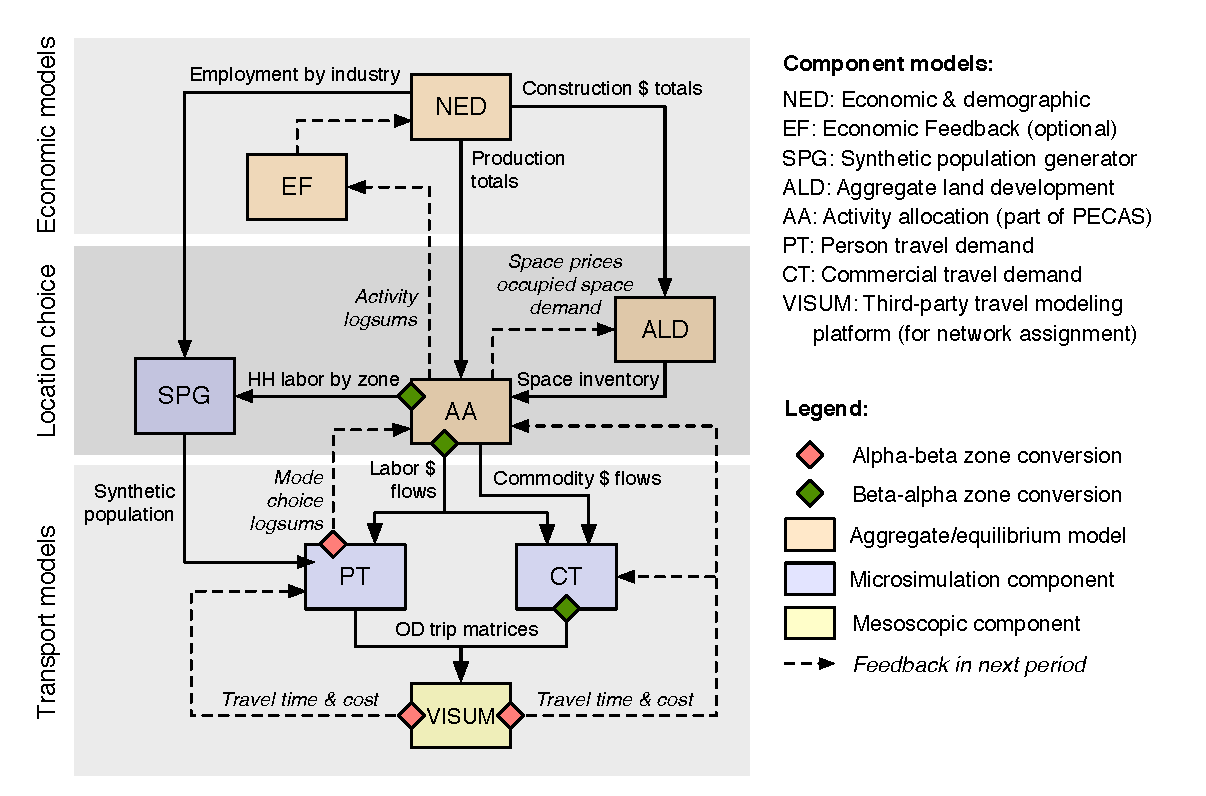
\includegraphics[scale=0.75, trim=1mm 1mm 1mm 1mm, clip]{summary/swim25-schematic}  
\caption{Modules and flows in the second generation Oregon StateWide Integrated Model (SWIM2)}
\label{fig:tlumip-schematic}
\end{figure}

\noindent The basic functionality of the SWIM2 system has been calibrated using several approaches:
\begin{itemize}
\item A three-stage approach to the calibration of the model has been implemented. The various parameters in each module have been sorted into three categories (S1, S2, and S3), related to the three stages in the calibration when they are considered.
\item Real-world (observed) values for more than 20 module outputs were established and used as targets for completing the S2 (each modules in isolation) and initial S3 (full model) calibration.
\item Calibration for a 1998 base year and trends over time was completed and shared with the TLUMIP Peer Review Panel in June 2008. The CT and PT modules have undergone further updates and were re-calibrated in October 2010. The NED and AA components (replacing the original ED and PI modules) were updated, and the spatial models re-calibrated in August 2011.  
\end{itemize}

\noindent The following user interface improvements have been made to support the use of the SWIM2 system:
\begin{itemize}
\item Implementation of a Model Runner System Graphical User Interface (MrsGUI) for facilitating model use, such as scenario creation, starting and monitoring model runs, and facilitating scenario archiving.
\item Implementation of a database (VIZ DB and VIZ DB Micro) to house model zone, link and microsimulation outputs in standardized format, as well as a visualization tool (SWIMVIZ) that enables a user-friendly dynamic queries and visualization of the multi-year model output in maps and charts.
\item Maintenance of a SWIM2 User'��s Guide including instructions for installing and running the model on the ODOT State Data Center (SDC) computer cluster, as well as other user information and instructions.
\end{itemize}

\noindent With this document and associated software, the SWIM2 functionality has been finalized and calibrated, and is ready for policy application. The following activities were undertaken to reach this outcome:
\begin{itemize}
\item All modules are completed as documented in this Guide, including software and inputs.
\item Software was developed in order to implement the full modeling system as specified, as confirmed through testing and calibration.
\item The values for the all parameters for each module have been developed, with many estimated statistically.
\item Base year inputs for all modules have been developed or synthesized, including the auto and transit networks.
\end{itemize}

% Note the references in the following paragraph

\noindent The SWIM2 system has the following advantages over the first generation SWIM1 model, completed in 1999 and implemented in the TRANUS platform \citep{donnelly99}: 
\begin{itemize}
\item Endogenously-generated regional economic forecasts, based on exogenous national forecasts, using the NED module.
\item More comprehensive aggregate treatment of regional economic flows (AA module), including explicit representation of commodities separate from industries and explicit treatment of related exchange locations and exchange prices.
\item Separation of management (white-collar) and production (blue-collar) components of production activities and the associated separation of consumption of these activities.
\item Much greater number of economic sectors considered in the economic and activity allocation modules (38 sectors, plus 14 white-collar/light-heavy industry sub-sectors, compared to 12 in SWIM1), as well as two non-household institutions.
\item Consideration for significantly more goods commodities (39 compared to 12 in SWIM1), as well as services and labor occupations.
\item Much greater number of space categories considered in land development and in production and consumption activity allocation (18 categories compared to 2 in SWIM1).
\item More intuitive zoning input used in land development (ALD), with 31 zoning codes.
\item Micro-level simulation of population (SPG module).
\item Much greater number of household sectors considered in activity allocation (AA module), stratified by household size as well as income group (18 compared to 3 in SWIM1).
\item Microsimulation of daily travel for nearly 6 million people within the study area (PT module).
\item Microsimulation of daily freight movements, including trans-shipment centers (CT module) and a wider range of vehicle types and related configurations.
\item Improved geographic coverage, including internal modeling of a roughly 50-mile halo region around the state of Oregon, which has as much activity as the state itself.
\item Significantly more detailed zones (2,950 alpha zones and 518 beta zones, compared to 125 zones in SWIM1) and networks (over 53,000 links, compared to nearly 2,000 in SWIM1).
\item Significantly higher temporal resolution options with time increments of one year, rather than five-year intervals in TRANUS.
\item Implementation of a distributed computing approach to help reduce run times for the SWIM2 modeling system.
\end{itemize}
\chapter{System Overview}
This report describes the working version of SWIM2 and its component modules, including data and calibration. This introduction describes the overall simulation system. It defines terms used often in the report, as well as the general calibration approach used in model development. The following chapters describe the individual model components. Within each discussion of them there are sections describing its design, to include equations and processes used. The estimation or synthesis of parameters and their values are described, as well as required model inputs. Sections describing the calibration process and outcomes are also included for each component.  

\section{Introduction}
The Oregon StateWide Integrated Model (SWIM2) is an integrated land use transport model covering the entire State of Oregon. It is a second generation model, drawing on previous work done on the first generation statewide model (SWIM1) and the Eugene-Springfield UrbanSim Model. The SWIM1 model \citep{parsons99} was a customized version of the TRANUS software\footnote{\url{http://www.tranus.com/tranus-english}}. SWIM2 is a more disaggregate and complex customized framework that combines a PECAS spatial allocation model with activity-based micro-simulation transport models. SWIM2 augments the SWIM1 Model in more complex applications of Oregon statewide policy and investment decisions. Future SWIM2 model upgrades will be driven by policy application needs.

The development of both the first and second generation models was commissioned by the Oregon Department of Transportation (ODOT) as part of its Transportation and Land Use Model Improvement Program (TLUMIP) within the larger Oregon Model Improvement Program (OMIP). The model development has been undertaken by a series of teams led by Parsons Brinckerhoff, with HBA Specto, EcoNorthwest and The University of Washington playing key roles as sub-contractors. The program has also been guided by an internationally prominent peer review panel.

The approach used in the development of SWIM2 has been to establish working versions and documentation of each of the modules shown in Figure \ref{fig:tlumip-schematic} (page \pageref{fig:tlumip-schematic}), before proceeding with full system integration. The preparation and testing of the software code, preparation of calibration and validation, establishing initial inputs and parameters and own-module calibration were completed first. Integration of the modules to run through time as a unit was completed next. Full model calibration of all modules in both a base year and trends overtime was completed and shared with the TLUMIP Peer Review Panel. Further calibration has and will continue to be performed as needed to match newer data and ensure the model is best equipped to address ODOT policy applications. 

The model is run in policy application mode for the period 2006-2030. The model steps through time in one-year intervals. The economic and spatial activities models --- the NED, SPG, ALD, and AA modules shown in Figure \ref{fig:tlumip-schematic} (page \pageref{fig:tlumip-schematic}) --- are run each year, while the transport models are only run every third year to reduce the time required to complete the entire simulation. The models were developed with an initial emphasis on reliability and ability to be easily understand and refactored. Subsequent versions of the models have been or will be tuned to achieved faster runtime performance.

% Removed Table 1, as it offered obsolete information at best

\section{Common modeling framework}
A great deal of data and information is shared by all components in the SWIM2 system. This includes model area category definitions, the Application Orchestrator (AO) module, and the overall calibration approach. Detailed descriptions of the user interface modules can be found in the SWIM2 User's Guide\footnote{https://github.io/tlumip/swim25/doc/userguide-v3.pdf}.

\subsection{Model area geography}\label{sec:model-area-geography}
The SWIM2 system operates at two geographic levels within the modeled area, show in Figure \ref{fig:swim2-model-area}. Both encompass 36 counties within Oregon and 39 counties in adjacent states. The latter is commonly referred to as to halo area of the model. The halo encompasses a roughly 50-mile buffer around Oregon. A system of 2,950 alpha zones (light and dark lines in Figure \ref{fig:swim2-model-area}) is the most disaggregate zone system. These include 12 external stations, show in Table \ref{tab:external-stations} and Figure \ref{fig:swim2-external-stations}. These external stations serve as gateways to the the six world markets used to represent the world beyond the halo.

\begin{figure}[!t]    % Figure 2.1 (although mis-captioned in original)
\centering
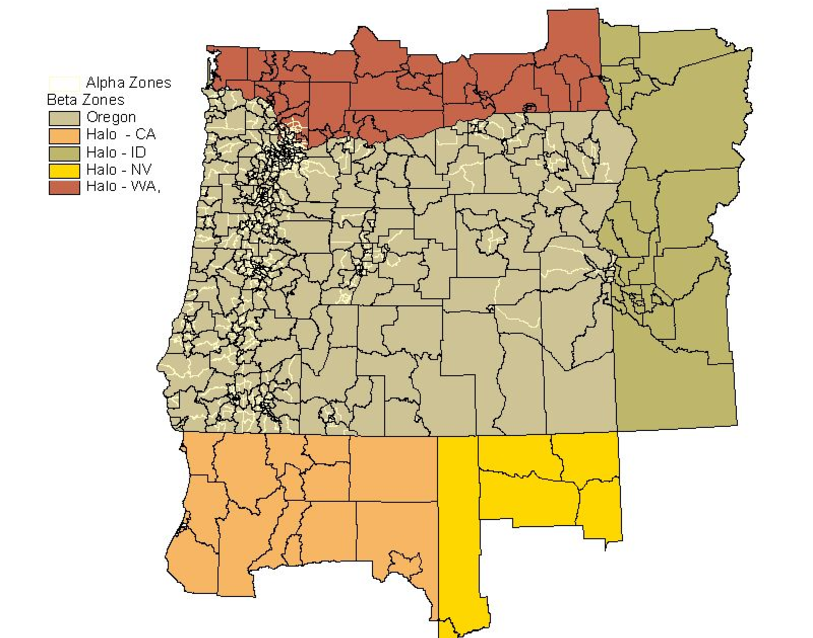
\includegraphics[scale=1.0]{overview/swim2-model-area}
\caption{SWIM2 modeled area zone system}\label{fig:swim2-model-area}
\end{figure}

\begin{table}
\centering
\caption{SWIM2 external stations}\label{tab:external-stations}
\begin{tabular}{cl|cl}
\hline
Alpha zone & External station & Alpha zone & External station \\
\hline
5001 & US101 (WA) & 5007 & I-84/US20 (ID) \\
\gray 5002 & I-5 (WA) & 5008 & US95 (NV, just north of I-80) \\
5003 & I-82 (WA) & 5009 & US395 (CA, just north of I-80) \\
\gray 5004 & US395/WA17 (WA) & 5010 & I-5 (CA) \\
5005 & US195 (WA) & 5011 & US101 (CA) \\
\gray 5006 & US95 (ID near WA border) & 5012 & Port of Portland Terminal 6 \\
\hline
\end{tabular}
\end{table}

\begin{figure}[!t]
\centering
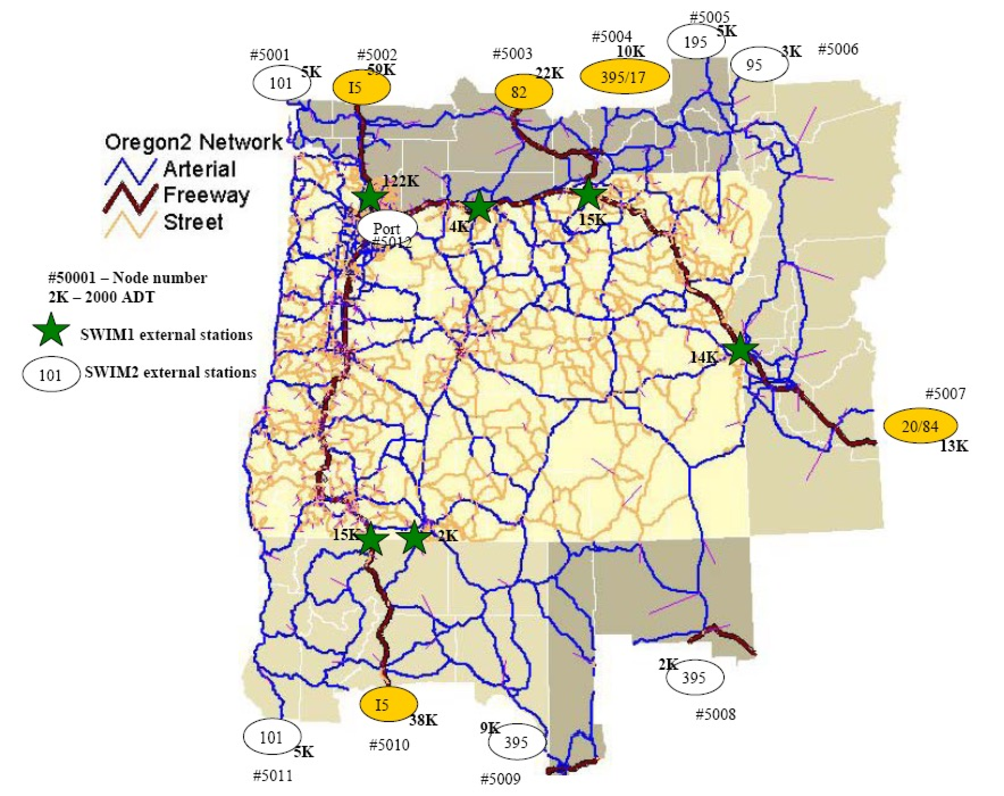
\includegraphics[width=6.25in]{overview/external-stations}
\caption{SWIM2 external stations}
\label{fig:swim2-external-stations}
\end{figure}
 
The activity allocation (AA) module operates on a more aggregated beta zone system (dark lines in Figure \ref{fig:swim2-model-area}), where the 12 external stations are replaced by six world markets listed in Table \ref{tab:world-markets}. There are 518 beta zones, collapsing zones only within Oregon, with a focus on the small urban zones. For example, the roughly 970 alpha zones in Portland are collapsed to approximate a set of 66 employment regions used by the Metro MPO model. In other urban areas, zones were collapsed based on a sliding population scale (approximately 25,000 persons per zone), respecting similar employment clusters and transportation commute sheds. In rural areas, homogenous public lands (e.g., BLM, National Forests) were collapsed, while retaining most county and all Area Commissions on Transportation (ACT) boundaries.\footnote{The ACTs are used in Oregon transportation planning, and provide a convenient way to divide the State into 12 areas.}

\begin{table}   % Table 2-2
\centering
\caption{AA world market zones and distance assumptions}
\label{tab:world-markets}
\begin{threeparttable}
\begin{tabular}{ccccl}
\hline
Zone & \multirow{2}{*}{Code} & Distance & External & \multirow{2}{*}{Definition} \\
number & & beyond halo\tnote{a} & station(s) & \\
\hline
6001 & N & 453/510 & 5002 & Washington and Canada \\
\gray6002 & NE & 453/510 & 5003, 5004 & Northern states of the Midwest \\
6003 & E & 1,661/1,399 & 5007 & Central and Eastern USA \\
\gray 6004 & S & 1,977/1,799 & 5010 & California, Southwestern states, Mexico \\
6005 & Ocean & 1500/600 & 5012 & Rest of the world\tnote{b} \\
\gray 6006 & Local & 75/75 & Non-Interstate & Local markets in neighboring states \\
\hline
\end{tabular}
\begin{tablenotes}
\footnotesize
\item[a] FHWA FAF3 distance data. Assumed 50 mph beyond halo to calculate equivalent travel time.
\item[b] Assumes \$600-900 import and \$700-2200 export costs to ship a Truck Equivalent Unit (TEU) between Portland and Japan (per May 2007 discussions with Port of Portland Staff). 
\end{tablenotes}
\end{threeparttable}
\end{table}

The six world markets defined in Table \ref{tab:world-markets} are only used only in the AA module. The direction of flow associated with them are shown in Figure \ref{fig:world-markets}, including the assumed distances to reach them beyond the model halo boundary. It is assumed that goods transported by truck and rail are limited to the US (except Hawaii), Canada, and Mexico. Imports and exports to other regions in the world are shipped by barge, either from the Port of Portland or other marine ports in the East or Southeastern regions of the USA. 

\begin{figure}   % Figure 2.3
\quote{\centering\small Note that the four directions shown refer to the directions N, NE, E, and S in\\Table \ref{tab:world-markets}. The shaded areas correspond to the areas each external market.\\}
\centering
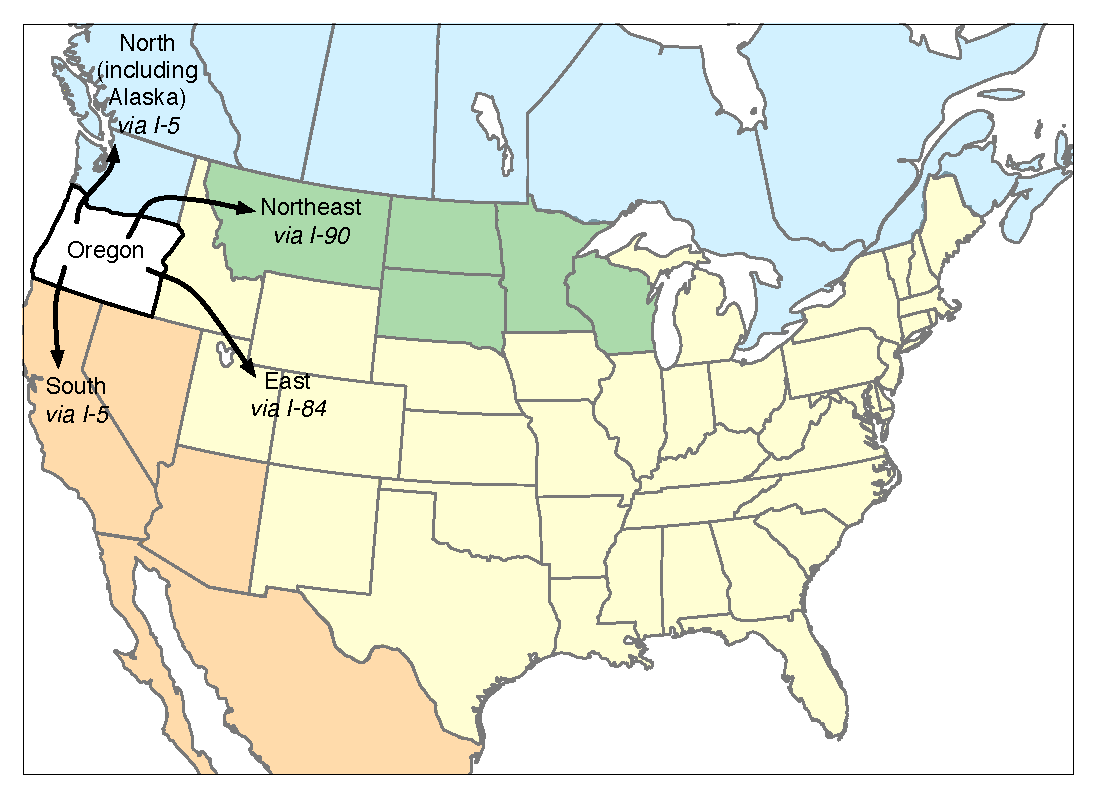
\includegraphics[width=5in]{overview/oregonregions}
\caption{Direction and extent of external and world markets in the SWIM2 system}
\label{fig:world-markets}
\end{figure}

The distances shown in Figure \ref{fig:world-markets} are based upon the Freight Analysis Framework (FAF)\footnote{\url{http://www.ops.fhwa.dot.gov/freight/freight_analysis/faf/}} Version 3.5 for truck flows and the truck portion of international intermodal flows. Data from the FAF base year of 2007 were used for these analyses. The approach described by \cite{moeckel10} was used for this purpose, assuming Euclidean distance between FAF zone centroids, with an additional distance added beyond the border in Canada (100 miles) and Mexico (300 miles). The distances within the model area, ranging from 90 to 425 miles (see Table 5 in \cite{moeckel10}), where excluded. In the case of the Oceanic market (zone 6005), an equivalent distance was identified that would result in the correct overall shipping costs, which varies by direction. The ``local'' world market (zone 6006) is assumed to support commodities that are traded within 75 miles of the model area.\footnote{The assignment of external origin/destination regions to external stations is based on a fastest travel time analysis to the centroids of each external region. An assumed average speed of 50 mph is used to calculate the equivalent travel time. World Market 6005 assumes an equivalent distance that allows accurate oceanic shipping costs, while using truck transport cost per mile as defined elsewhere in the AA module (CommoditiesI.csv). Oceanic time costs were assumed to be zero, as goods sent by ship tend to be less time-dependent. The air freight mode was ignored, as it represents less than one percent of all goods movement in Oregon, and at most two percent of any single commodity's flows.}

These six world markets link to the model transport network at the 12 external stations shown in Figure \ref{fig:swim2-external-stations} and Table \ref{tab:external-stations}. These external stations roughly parallel the likely rail as well as truck freight routes entering and leaving the model area. The local world market (zone 6006), trading within 75 miles of the model boundary, is linked to the minor roadway external stations, which consists of the non-Interstate highways shown in the Table.\footnote{Flows to and from World Market 6006 within 75 miles of the model border are currently not assigned, as they represent less than four percent of overall goods flows.}

% Figure 2.4 World Markets outside US (never referenced in the text, so omitted)

The aggregate land development (ALD) component uses a 15-region aggregation of the alpha zones for making land development decisions. These regions, shown in Figure \ref{fig:ald-regions}, represent SWIM2 land development markets within the study area.

\begin{figure}[!t]
\centering
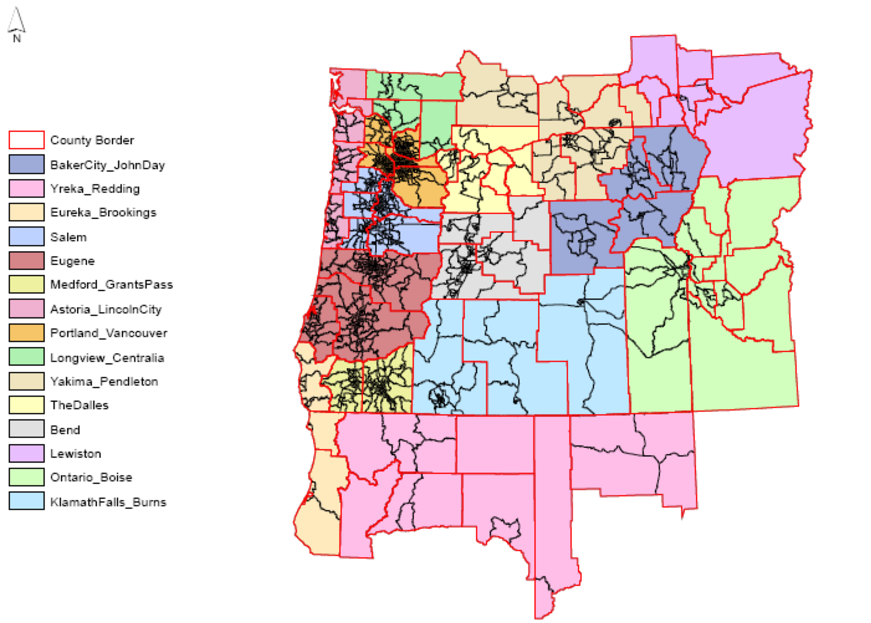
\includegraphics[width=6.25in]{overview/ald-regions}
\caption{Aggregate land development (ALD) regions}
\label{fig:ald-regions}
\end{figure}

\subsection{Category definitions}\label{sec:category-definitions}
At its core the SWIM2 system encapsulates a spatial input-output (IO) formulation that resides in the AA component. A summary of the IO make and use table framework and the categories of activities and commodities used within them is shown in Figure \ref{fig:make-use-summary}. The Figure shows the specific types of economic interactions represented in the model. Commodity production is represented in the make table at the top of the Figure. Commodity consumption is represented in the use table at the bottom of the Figure. Commodities flow down the columns from where they are produced to where they are consumed. The general nature of the exchange location for each commodity category and the treatment of imports and exports are also indicated.

The industry, government and household activity categories used in SWIM2 are shown in Tables \ref{tab:activity-industry} and \ref{tab:size-income}. Certain industries have been allowed to use more than one space type, exploiting new AA routines that calculate zonal size terms based on quantities of space, and so is better able to allocate activities in zones with limited space-type availability. Some activities are classified based upon the North American Industrial Classification System (NAICS)\footnote{\url{http://www.census.gov/eos/www/naics/}}, while others are grouped together to define land use, transport, or labor markets (e.g., Services-At Customers Business, Services-Storefront). In general, a given industrial sector is split into blue-collar and white-collar (or ``office support'') components using associated production and office space categories, respectively. In this way the allocation processes in the AA component can consider the very different location behavior and space requirements of these two categories. Internal office support activities strictly produce management services consumed by their corresponding industries. For instance, Services at customer's house are self-employed workers who sell their services to households (e.g., housekeepers, nannies, handymen).

\begin{sidewaysfigure}     % Figure 2-6
\centering
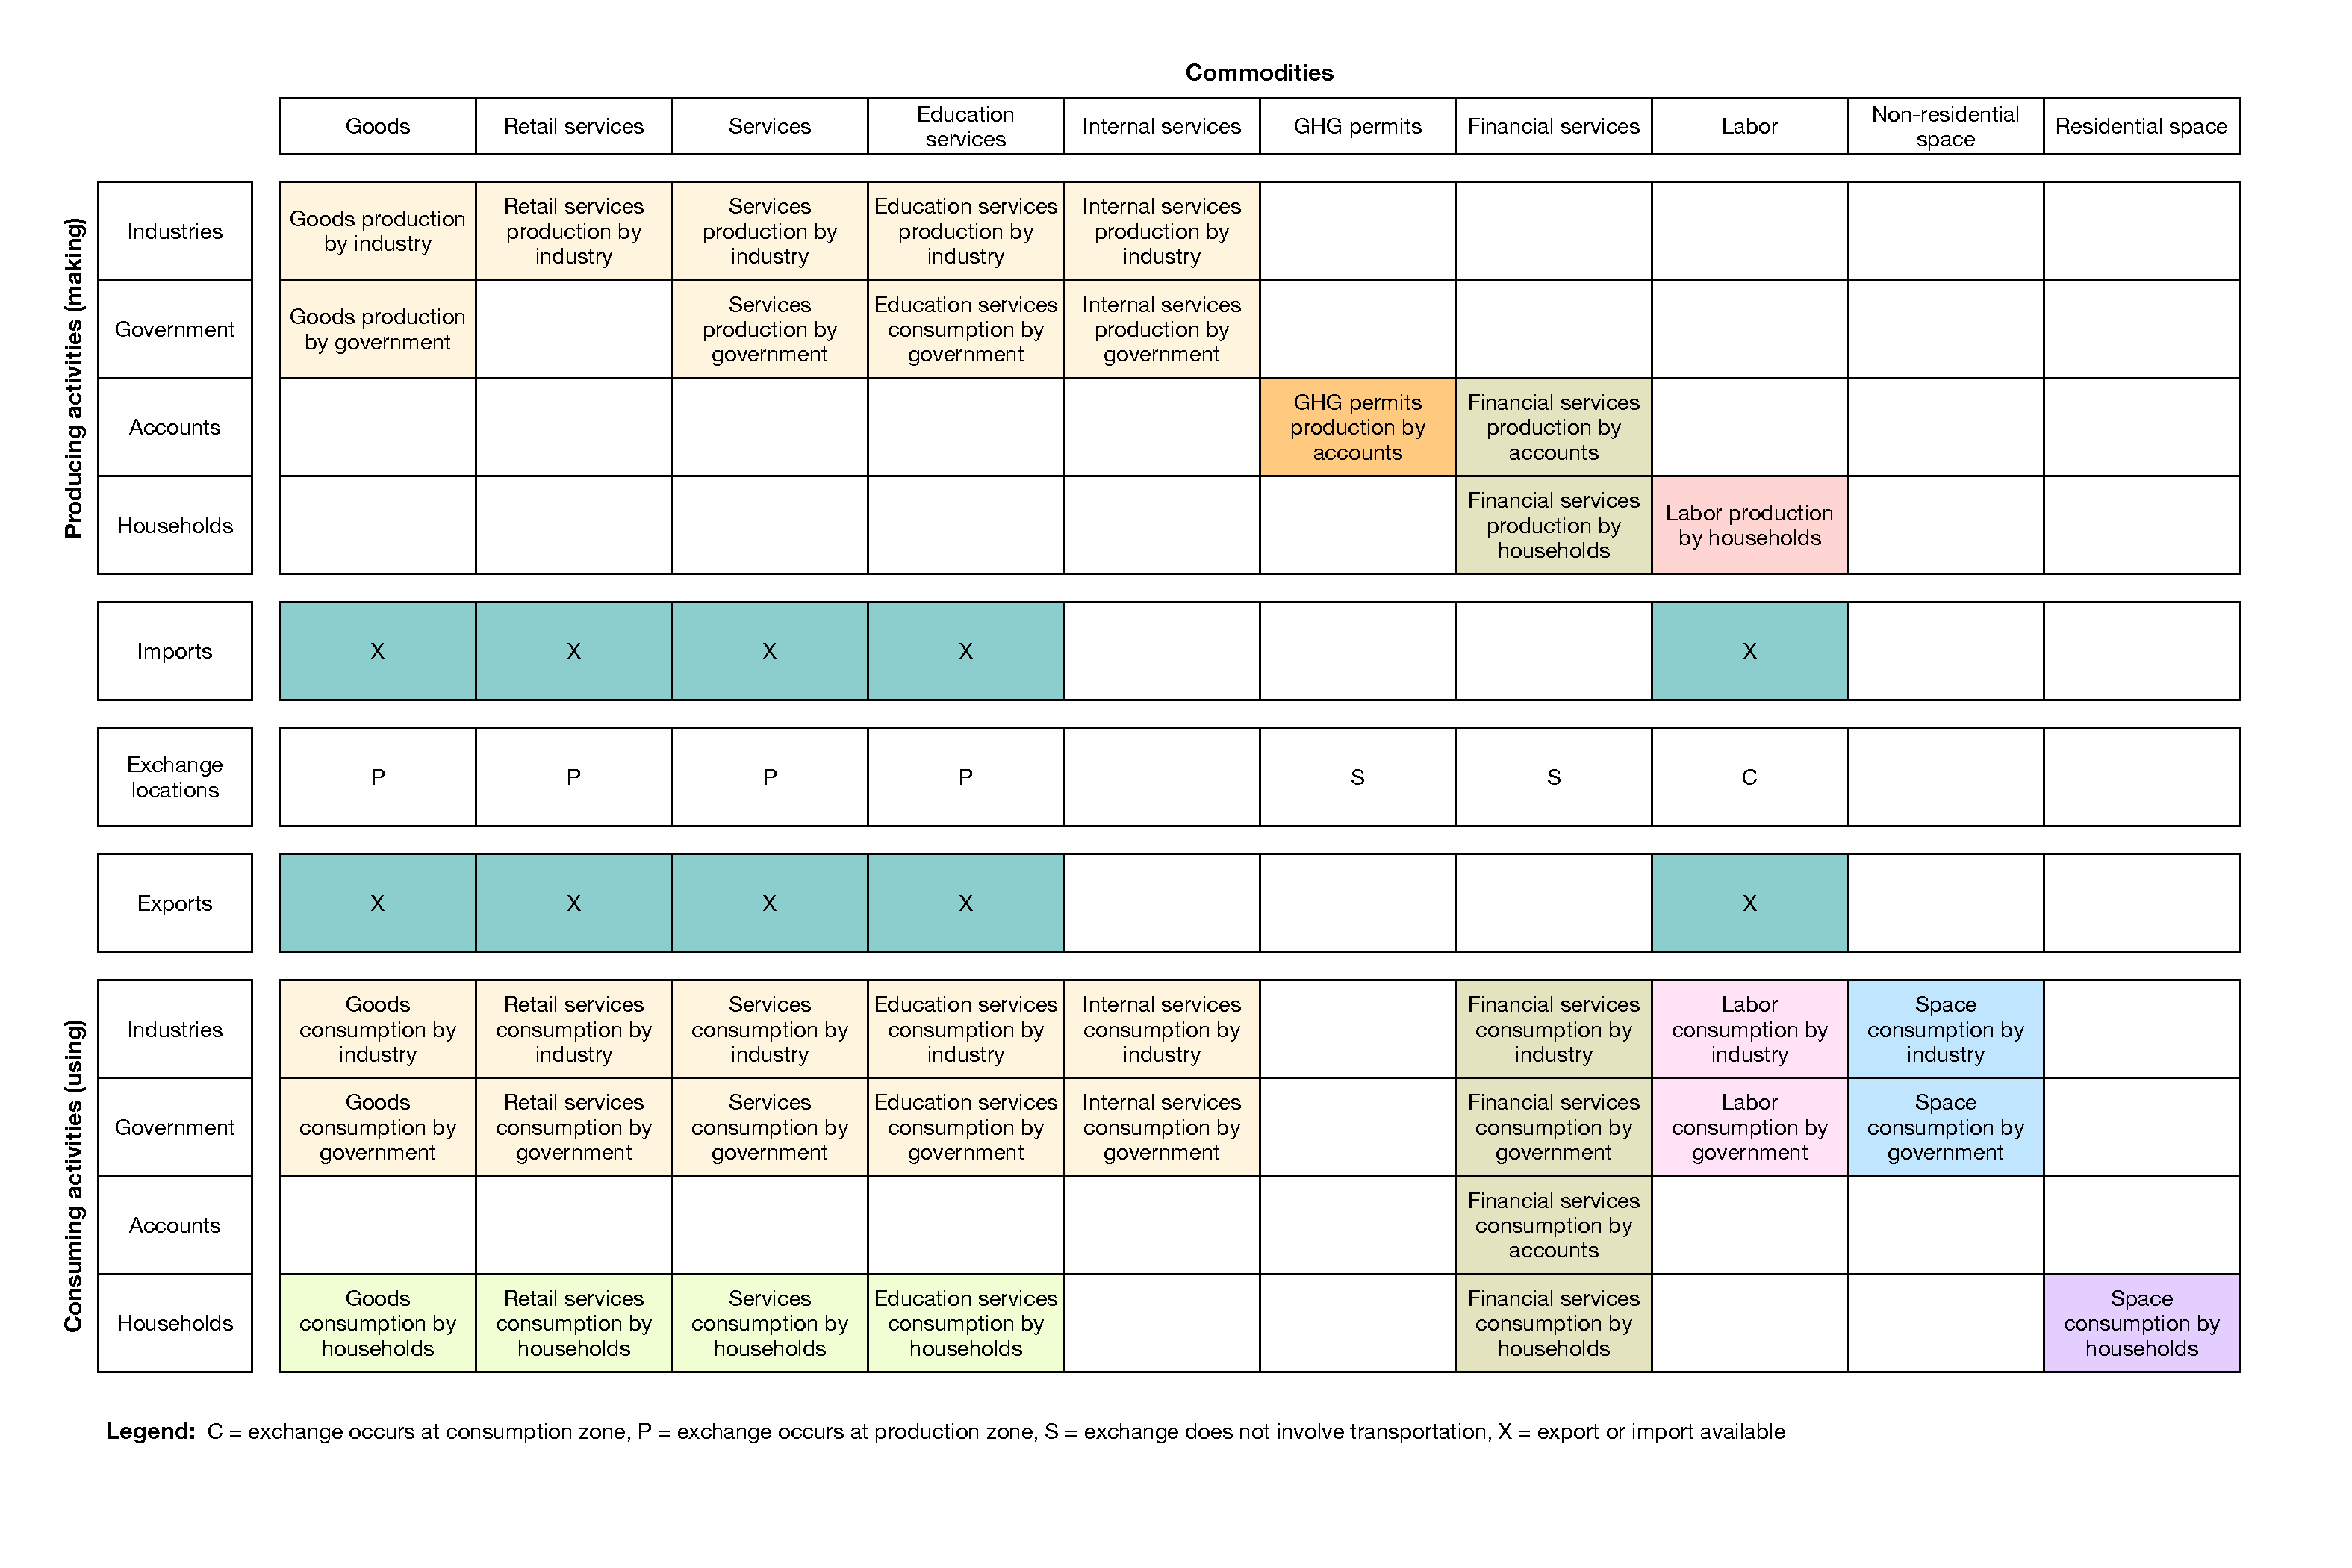
\includegraphics[scale=0.45]{overview/make-use-summary}
\caption{Summary of commodities made and used by various activities within the model}
\label{fig:make-use-summary}
\end{sidewaysfigure}

% Table 2-3 in v29
\begin{table}
\centering
\caption{Activities by industry}\label{tab:activity-industry}
\fontsize{9.5}{10.5}\rm
\begin{tabular}{|l|l|l|}
\hline
Industry                        & Floorspace options & Internal services \\
\hline
Resource-Ag and Mining          & FLR Agriculture & Internal Services Resources \\
Resource-Forest                 & FLR Logging & Internal Services Resources \\
Resource Office Support         & FLR Office & \\
\hline 	
Energy-Electric                 & FLR Heavy Industry & Internal Services Energy \\
Energy-Natural Gas              & FLR Heavy Industry & Internal Services Energy \\
Energy-Petroleum                & FLR Heavy Industry & Internal Services Energy \\
Energy Office Support           & FLR Office &  \\
\hline
Utilities-Other                 & FLR Office, FLR Light Industry & Internal Services Utilities \\
Utilities-Other Office Support  & FLR Office &  \\
\hline
Construction-Maintenance        & n/a & Internal Services Construction \\
Construction-Nonresidential     & n/a & Internal Services Construction \\
Construction-Other              & n/a & Internal Services Construction \\
Construction-Residential        & n/a & Internal Services Construction \\
Construction Office Support     & n/a & \\
\hline
Manufacturing-Food HI           & FLR Heavy Industry & Internal Services Manufacturing \\
Manufacturing-Food LI           & FLR Light Industry & Internal Services Manufacturing \\
Manufacturing-High Tech HI      & FLR Heavy Industry & Internal Services Manufacturing \\
Manufacturing-High Tech LI      & FLR Light Industry & Internal Services Manufacturing \\
Manufacturing-High VTW HI       & FLR Heavy Industry & Internal Services Manufacturing \\
Manufacturing-High VTW LI       & FLR Light Industry & Internal Services Manufacturing \\
Manufacturing-Low VTW HI        & FLR Heavy Industry & Internal Services Manufacturing \\
Manufacturing-Wood and Paper HI & FLR Heavy Industry & Internal Services Manufacturing \\
Manufacturing Office Support    & FLR Office & \\
\hline
Information                     & FLR Office & Internal Services Information \\
Information Office Support      & FLR Office, FLR Light Industry & \\
\hline
Wholesale                       & FLR Warehouse & Internal Services Wholesale \\
Wholesale Office Support        & FLR Office & \\
\hline
Transport                       & FLR Warehouse & Internal Services Transport \\
Transport Office Support        & FLR Office &  \\
\hline
Retail-Automotive               & FLR Retail &  \\
Retail-Store                    & FLR Retail & Internal Services Retail Store \\
Retail-Store Office Support     & FLR Office &  \\
Retail-Nonstore                 & FLR Office &  \\
\hline
Finance and Insurance           & FLR Office &  \\
Real Estate                     & FLR Office &  \\
\hline
Entertainment                   & FLR Retail &  \\
Accommodations                  & FLR Accommodation &  \\
Eating and Drinking Places      & FLR Retail, FLR Accommodation &  \\
Services-Professional and Technical & FLR Office &  \\
Services-at Customer's Business & FLR Light Industry &  \\
Services-at Customer's House    & n/a &  \\
Services-Business               & FLR Office &  \\
Services-Nonprofit              & FLR Office, FLR Institutional &  \\
Services-Storefront             & FLR Retail &  \\
\hline
Health-Hospital                 & FLR Hospital &  \\
Health-Care Facility            & FLR Institutional &  \\
Health-Other                    & FLR Office, FLR Light Industry &  \\
\hline
Education-K12                   & FLR K12 & Internal Services Education K12 \\
Education-K12 Office Support    & FLR Office &  \\
Education-Higher                & FLR Office, FLR Institutional &  \\
\hline
Government Administration Operations & n/a & Internal Services GovAdmin \\
Government Administration Office Support & n/a &  \\
\hline
\end{tabular}
\end{table}    % Table 2.3
% Table 2-4 in v29
\begin{table}
\centering
\caption{Household size and income categories (2009 dollars)}\label{tab:size-income}
\fontsize{11.0}{13.75}\rm
\begin{tabular}{lcl}
\hline
Code & Household income & Household size \\
\hline
HH0to8k1to2 & \$0 to 7,999 & 1 to 2 persons \\
\gray HH0to8k3plus & \$0 to 7,999 & 3 or more persons \\
HH8to15k1to2 & \$8,000 to 14,999 & 1 to 2 persons \\
\gray HH8to15k3plus & \$8,000 to 14,999 & 3 or more persons \\
HH15to23k1to2 & \$15,000 to 22,999 & 1 to 2 persons \\
\gray HH15to23k3plus & \$15,000 to 22,999 & 3 or more persons \\
HH23to32k1to2 & \$23,000 to 31,999 & 1 to 2 persons \\
\gray HH23to32k3plus & \$23,000 to 31,999 & 3 or more persons \\
HH32to46k1to2 & \$32,000 to 45,999 & 1 to 2 persons \\
\gray HH32to46k3plus & \$32,000 to 45,999 & 3 or more persons \\
HH46to61k1to2 & \$46,000 to 60,999 & 1 to 2 persons \\
\gray HH46to61k3plus & \$46,000 to 60,999 & 3 or more persons \\
HH61to76k1to2 & \$61,000 to 75,999 & 1 to 2 persons \\
\gray HH61to76k3plus & \$61,000 to 75,999 & 3 or more persons \\
HH76to106k1to2 & \$76,000 to 105,999 & 1 to 2 persons \\
\gray HH76to106k3plus & \$76,000 to 105,999 & 3 or more persons \\
HH106kUp1to2 & \$106,000 and over & 1 to 2 persons \\
\gray HH106kUp3plus & \$106,000 and over & 3 or more persons \\
\hline
\end{tabular}
\end{table}      % Table 2.4

Other considerations in the classification of industries include:
\begin{itemize}
\item The distributors and generators of energy used in buildings (natural gas distribution, electrical power generation transmission and distribution, and petroleum) were separated into three subcategories to support better representation of energy use and associated greenhouse gas emissions. Construction was divided into residential buildings, non-residential buildings, maintenance, other buildings and office support, to better support the ALD component.
\item Food, wood and paper, and high technology remain as separate manufacturing sectors but, were divided into heavy industry and light industry. The remaining manufacturing sectors were divided based on the value-to-weight ratio of their production, to separate those dependent on the movement of heavy goods in large trucks and by rail. They were also split into heavy and light industry categories.
\item Wholesale and retail are two separate categories. The first one was split into Wholesale and Wholesale Office Support. The retail category was split into four subcategories: Automotive, Store, Store Office Support and Non-store.
\item Transportation, Information, and Utilities are three separate categories. Each of them was split into two in order to represent the management of the service, using a subcategory of Office Support.
\item Finance and Insurance, and Real Estate remain as separate categories.
\item Health as category includes three subcategories: Hospitals, Care Facility and Other.
\item Three subcategories can be found in Education: Education-K12 (previously called Grade-school), Education Office Support and Higher Education.
\item Entertainment, Accommodations and Eating and Drinking places are separate sector industries.
\item Services as a sector industry was split based on two criteria: the space type they use and the NAICS two-digit industry categories. In the first group are three subcategories: Services-At Customer's Business, Services-At Customer's House, and Services-Storefront. In the second group are: Services-Professional and Technical, Services-Business and Services-Non-profit.
\item For government administration category two subcategories were set-up: Operations and Office Support.
\end{itemize} 

Household activities were classified as categories of household income and size (persons per household) based on the original 1990 Census definitions, inflated to 2009 dollars using prices index for gross domestic product (GDP) from the Bureau of Economic Analysis (BEA) of the U.S. Department of Commerce. Household activities include the production of labor and consumption of various goods (primarily through retail) and services. Household income groups reflect the original SWIM2 1990 Census categories, with income amounts inflated to 2009 dollars (consistent with the 2010 census and 2009 IMPLAN) using a 1.52 GDP deflator.

Group quarters (GQ) are represented in SWIM2 using the same definitions used in the 2005-09 American Community Survey (ACS)\footnote{\url{http://www.census.gov/acs/www/}}. They represent six percent of all Oregon households, evenly split between institutional and non-institutional (e.g., student) populations. In a summary of the 2009 ACS PUMS it was found that half of the GQ residents are in institutions. The other half, which includes students, consists mainly of 1--2 person multi-family households.

The commodities produced and consumed in the model, including study area imports and exports, are shown in Table \ref{tab:goods-categories}. Industry and government activities include the production and consumption of goods and services. The commodities shown in the Table are tracked in the AA and commercial travel (CT) components, including 39 types of goods based on the Standard Classification of Transportable Goods (SCTG) categories\footnote{\url{https://www.census.gov/svsd/www/cfsdat/cfs071200.pdf}}. Energy flows, to include natural gas and electricity, were added so that their levels could be tracked. However, since these energy sources are not transported by truck they are not explicitly addressed in the CT module. In addition, within AA two commodities are combined in order to eliminate small and problematic tobacco (SCTG 9) shipments and to avoid splitting the sand and gravel industries (SCTG 11 and 13). The full set of SCTG file outputs will still be produced by AA, but one will have zero flows. This enables their explicit treatment within AA without accompanying changes in the CT module.

\begin{table}   % Table 2-6
\centering
\caption{Commodities---goods categories}\label{tab:goods-categories}
\small
\begin{tabular}{ll}
\hline
SCTG code & Description \\
\hline
SCTG1\_FKP\_L VSK & Live Animals and Fish \\
\gray SCTG2\_FKP\_AGRI\_cereal & Cereal Grains (including seed) \\
SCTG3\_FKP\_AGRI\_other & Other Agricultural Products, except for Animal Feed \\
\gray SCTG4\_FKP\_FEED & *Animal Feed and Products of Animal Origin, n.e.c. \\
SCTG5\_FKP\_FOOD\_meat & *Meat, Fish, and Seafood, and Their Preparations \\
\gray SCTG6\_FKP\_AGRI\_grain & *Milled Grain Products and Preparations, and Bakery Products \\
SCTG7\_FKP\_FOOD\_prep & *Other Prepared Foodstuffs, and Fats and Oils \\
\gray SCTG8\_FKP\_FOOD\_alc & *Alcoholic Beverages \\
SCTG9\_FKP\_FOOD\_tob & Tobacco Products \\
\gray SCTG10\_CMS\_CLAY & Monumental or Building Stone \\
SCTG11\_CMS\_SAND & Natural Sands \\
\gray SCTG12\_CMS\_STON & Gravel and Crushed Stone \\
SCTG13\_CMS\_MINE\_nonmet & Non-Metallic Minerals, n.e.c. \\
\gray SCTG14\_CMS\_MINE\_met & Metallic Ores and Concentrates \\
SCTG15\_PCC\_COAL & Coal \\
\gray SCTG16\_PCC\_PETR\_crude & Crude Petroleum Oil \\
SCTG17\_PCC\_FUEL & *Gasoline and Aviation Turbine Fuel \\
\gray SCTG18\_PCC\_PETR\_oil & *Fuel Oils \\
SCTG19\_PCC\_COAL\_prod & Coal and Petroleum Products, n.e.c. \\
\gray SCTG20\_PCC\_CHEM\_basic & Basic Chemicals \\
SCTG21\_PCC\_CHEM\_pharma & *Pharmaceutical Products \\
\gray SCTG22\_PCC\_CHEM\_fert & Fertilizers \\
SCTG23\_PCC\_CHEM\_prod & *Chemical Products and Preparations, n.e.c. \\
\gray SCTG24\_PCC\_PETR\_plast & Plastics and Rubber \\
SCTG25\_FWP\_LOGS & Logs and Other Wood in the Rough \\
\gray SCTG26\_FWP\_WOOD & Wood Products \\
SCTG27\_PPP\_P APR\_puplp & Pulp, Newsprint, Paper, and Paperboard \\
\gray SCTG28\_PPP\_P APR\_paper & Paper or Paperboard Articles \\
SCTG29\_PPP\_P APR\_print & *Printed Products \\
\gray SCTG30\_OTH\_CLTH & *Textiles, Leather, and Articles of Textiles or Leather \\
SCTG31\_CMS\_MIN & Non-Metallic Mineral Products \\
\gray SCTG32\_MIT\_METL\_base & Base metal in primary or semi-finished forms and in finished basic shapes  \\
SCTG33\_MIT\_METL\_prod & Articles of Base Metal \\
\gray SCTG34\_MIT\_MACH & Machinery \\
SCTG35\_MIT\_ELCT & Electronic, electrical, and office equipment and components \\
\gray SCTG36\_MIT\_TRAN & *Motorized and Other Vehicles (including parts) \\
SCTG37\_MIT\_INST\_transp & Transportation Equipment, n.e.c. \\
\gray SCTG38\_MIT\_INST\_prec & Precision Instruments and Apparatus \\
SCTG39\_OTH\_FURN & *Furniture and fixtures and lighting and illuminated signs \\
\gray SCTG40\_OTH\_MISC & *Miscellaneous Manufactured Products \\
SCTG41\_WASTE\_SCRAP & Waste and Scrap \\
\hline
\end{tabular}
\end{table}

The services tracked in the AA and person travel (PT) modules are shown in Table \ref{tab:service-categories}. Internal services, defined as ``value-added office labor,'' spatially connect the production and office components of split industries. This commodity is the service provided by management and other office support workers to the production floor of the same industry. In many cases, this flow represents a relationship between two establishments of the same firm.

% Table 2-5 in v29
\begin{table}
\centering
\caption{Commodities and service categories}\label{tab:service-categories}
\fontsize{11.5}{14.375}\rm
\begin{tabular}{|l|l|}
\hline
Services category & Services included \\
\hline
Retail Services (p) & Retail Trade \\
\hline
Services & Energy (c) \\
 & Transport (p) \\
 & Wholesale Trade (p) \\
 & Construction (c) \\
 & Communications and Utilities (p) \\
 & Accommodations (p) \\
 & Personal and Other Services and Amusements (p) \\
 & Entertainment Services (p) \\
 & Food Services (p) \\
 & Health Services (p) \\
 & FIRE, Business, and Professional services (c) \\
 & Government Administration (p) \\
\hline
Education Services (p) & Teaching K12 \\
 & Higher Education \\
\hline
Environmental (s) & GHG Permits \\
\hline
Financial Services (s) & Government Support Receipts \\
 & Tax Receipts \\
 & Investing Receipts \\
 & Proprietor Income Receipts \\
 & Return Investment Receipts \\
 & Capital Transfer Receipts \\
 & Education Reports to Sponsors \\
\hline
Internal Services (c) & Internal Services Resources \\
 & Internal Services Energy \\
 & Internal Services Construction \\
 & Internal Services Manufacturing \\
 & Internal Services Wholesale \\
 & Internal Services Retail Store \\
 & Internal Services Transport \\
 & Internal Services Information \\
 & Internal Services Utilities \\
 & Internal Services Education K12 \\
 & Internal Services Government Administration \\
\hline
\end{tabular}
\end{table}  % Used to be Table 2-5, but mis-numbered because of duplicate Tables 2-6

Labor is included as a commodity that is produced by households and consumed by economic production activities. As such, the synthetic population generator (SPG) respects the home end while PT respects the work end of labor flows produced by the AA component. Different labor occupation categories from 2000 Standard Occupational Categories (SOC)\footnote{\url{http://www.bls.gov/soc/}} codes are treated as different commodity categories. Thirteen categories of labor have been defined considering occupations and years of education, as shown in Figure \ref{fig:labor-occupation-categories}. The new labor categorization is based on the following three principles:
\begin{itemize}
\item Four groups of two-digit SOC codes, for comparing with any data sources that summarize employment based on 2-digit SOC.
\item Within three of the four groups, the occupations requiring lower education (based on observed education levels in the ACS PUMS) were grouped together, with the idea that these workers would have a lower income, a lower value of time, and could more easily and more readily switch between two-digit SOC categories. These were named ``unskilled'' occupations, although of course in every occupation there are some highly skilled individuals.
\item Within the higher education occupations, occupations were further split into more detailed two-digit SOC groups.
\end{itemize}

\begin{figure}[!t]   % A figure that was labeled as one of several Tables 2-5
\centering
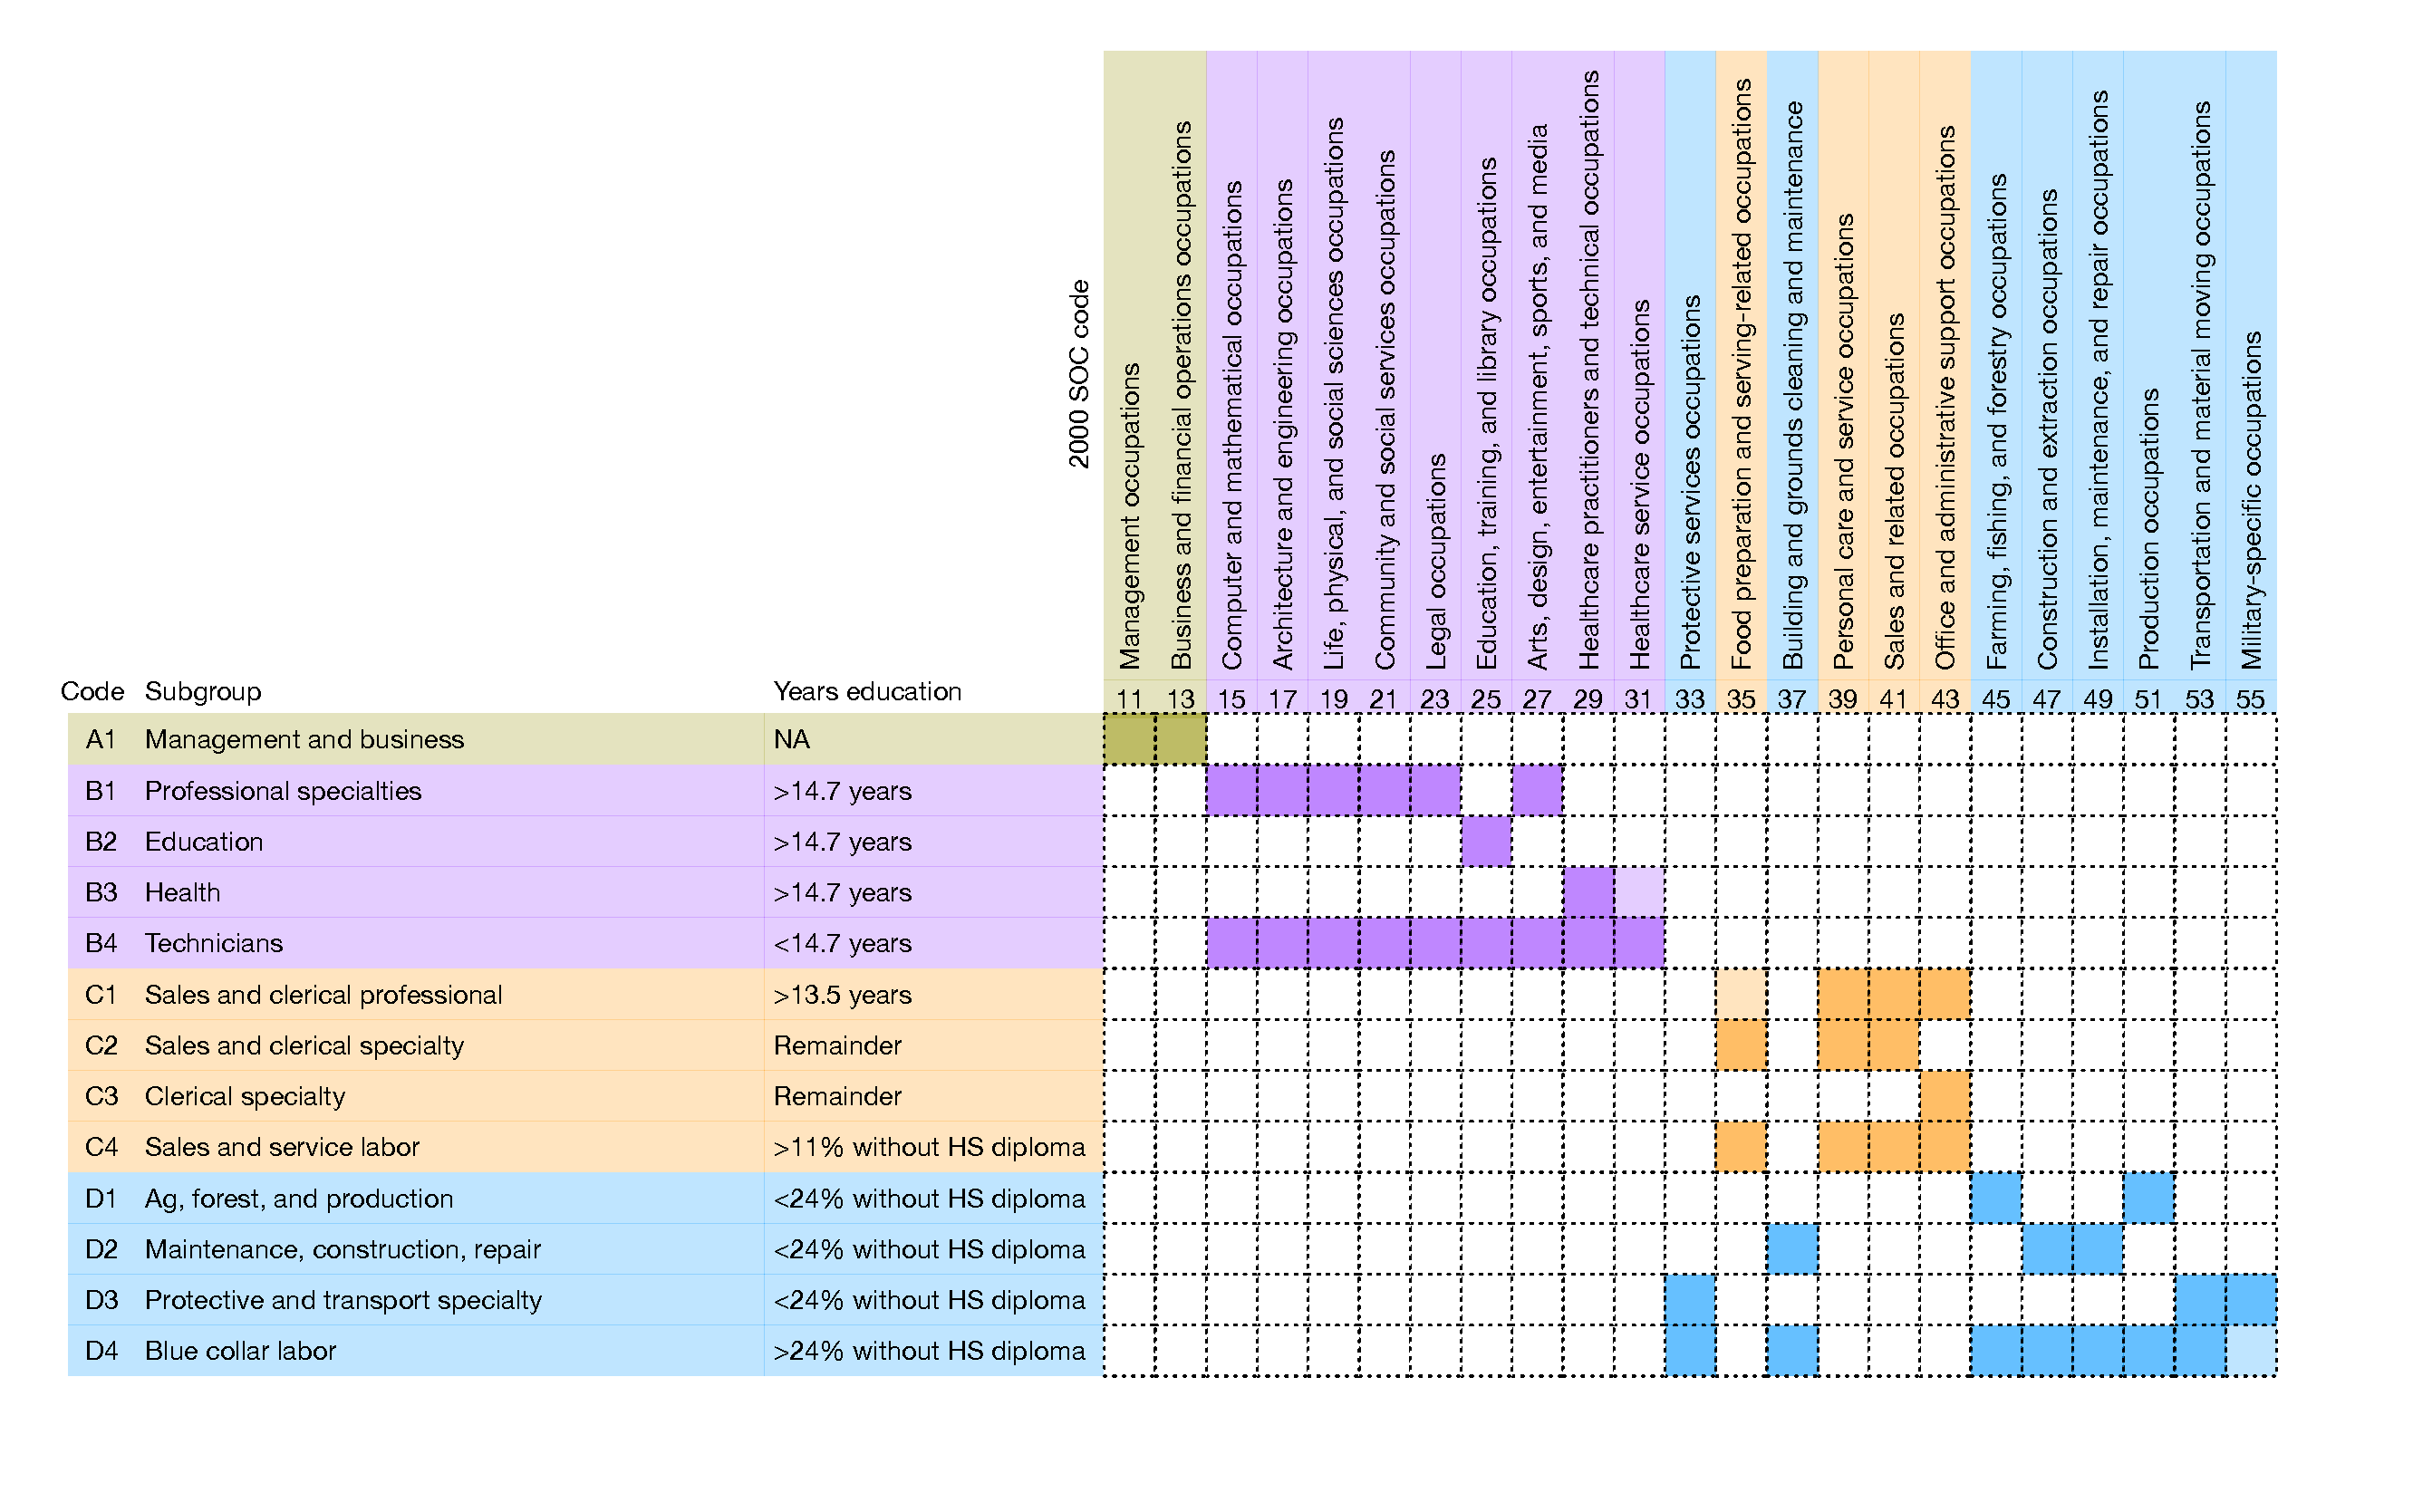
\includegraphics[scale=0.4, trim=11mm 23mm 0mm 0mm, clip]{overview/commodities-labor-categories}  % trim=l b r t
\caption{Labor occupation categories}\label{fig:labor-occupation-categories}
\end{figure}

Floorspace categories are shown in Table \ref{tab:floorspace-categories}, while Table \ref{tab:activity-industry} identifies which floorspace types are used by each industry category. ALD adjusts the inventory of developed floorspace available in alpha zones in each model period. The original FLR\_Depot space type was ambiguous, and has been combined with FLR\_Warehouse. Additionally, heavy and light industry spaces definitions have been updated slightly. Likely more light industry will be demanded, but is expected to be within the tolerance of ALD's current interpretation of zoning inputs.   

% Table 2-6 in v29
\begin{table}
\centering
\caption{Floorspace categories}\label{tab:floorspace-categories}
\fontsize{11.0}{13.75}\rm
\begin{tabular}{|l|l|l|}
\hline
Residential floorspace & Non-residential floorspace & Resource floorspace \\
\hline
FLR SFD (Single Family Home) & FLR Hospital & FLR Agriculture (includes Mining) \\
FLR AT (Attached Home) & FLR Retail & FLR Logging \\
FLR MH (Manufactured Home) & FLR Office & \\
FLR RRMH (Rural Residential MH) & FLR Heavy Industry & \\
FLR RRSFD (Rual Residential SFD) & FLR Light Industry & \\
FLR MF (Multi-family, Institutional) & FLR Warehouse & \\
 & FLR Institutional &  \\
 & FLR Accommodation & \\
 & FLR Government Support & \\
 & FLR K12 (Grade School) & \\
\hline
\end{tabular}
\end{table}   % Table 2-6

The various modes and vehicles used in the model to transport person and goods flows are shown in Table \ref{tab:transport-modes}. Non-motorized passenger modes and non-truck freight modes are not assigned to the network.

\begin{sidewaystable}
\centering
\caption{Transport modes and vehicle types}\label{tab:transport-modes}
\begin{tabular}{|l|l|l|l|c|}
\hline
Type & Code & Trip mode & Definition & Component(s) \\
\hline
Person & DA & Drive alone & Single-occupant auto & SDT, LDT \\
\gray \cellcolor{white}travel & SR2 & Shared ride 2 & Two-occupant auto & SDT, LDT \\
 & SR3P & Shared ride 3+ & Three or more occupant auto & SDT, LDT \\
\gray \cellcolor{white}& WALK & Walk & Walk & SDT \\
 & BIKE & Bicycle & Bicycle & SDT \\
\gray \cellcolor{white}& SCHOOL\_BUS & School bus & School bus (not assigned) & SDT \\
 & TRANSIT\_WALK & Walk to transit & Walk-access transit & LDT \\
\gray \cellcolor{white}& TRANSIT\_DRIVE & Drive to transit & Drive-access transit & LDT \\
 & AIR & Drive to air & Drive-access air travel within modeled area & LDT \\
\gray \cellcolor{white}& HSR\_DRIVE & Drive to HSR & Drive-access intercity rail & LDT \\
 & HSR\_WALK & Walk to HSR & Walk-access to intercity rail & LDT \\
\hline
\gray \cellcolor{white}Freight & TRK1 & Truck type 1 & $<$34,000 lbs. (likely single-unit) & CT, ET \\
 & TRK2 & Truck type 2 & 34,000--64,000 lbs. & CT, ET \\
\gray \cellcolor{white}& TRK3 & Truck type 3 & 64,000--80,000 lbs. (articulated) & CT, ET \\
 & TRK4 & Truck type 4 & 80,000--105,500 lbs. (articulated) & CT, ET \\
\gray \cellcolor{white}& TRK5 & Truck type 5 & $>$105,500 lbs. (articulated) & CT, ET \\
 & SAA & Air freight & Air freight (not assigned) & \\
\gray \cellcolor{white}& SRR & Rail freight & Rail freight (not assigned) & \\
 & SWA & Waterborne freight & Waterborne freight (not assigned) & \\
\gray \cellcolor{white}& SPA & Pipeline & Pipeline freight (not assigned) & \\
\hline
\end{tabular}
\end{sidewaystable}  % Table 2-7
 
The attributes of persons and households created in the SPG module and used in the PT module are shown in Figure \ref{fig:synthetic-attributes}. The Table also shows the 1990 Census-based coding categories for each attribute. The fields of the synthetic population used in the SWIM2 model are described below, with synthesized value marked by asterisk. The others are retained from the drawn PUMS record. SPG controls only for workers per household, worker industry, and person age. SWIM2 assigns home location and work location based on AA labor flows:
\begin{itemize}
\item \textit{Household-Person File Link (HH\_ID, PER\_ID):} The household attributes were linked to each person in the household, by storing a household (HH\_ID) and person (PER\_ID) ID in the person file. HH\_ID are numbered sequentially across the whole sample, starting with 1. PER\_IDs are numbered sequentially across all persons in a household. 
\item \textit{Household Attributes (PERSONS, AUTOS*):} The number of persons and the total number of autos in the household. The Census auto value is updated by the PT module.
\item \textit{Home Location (AZONE):} The alpha zone location of the household, assigned by SPG2, consistent with AA labor flows by occupation. 
\item \textit{Household Income (RHHINC):} Total household income in units of 2009 dollars.
\item \textit{Residential Floorspace Type (UNITS1, SINGLE\_FAMILY*):} The household's residential floor\-space type is indicated by the number of units in the dwelling unit (UNITS1). In PT, a binary variable is created to indicate whether the dwelling unit is a single family unit. 
\item \textit{Demographics (AGE, SEX):} Age and gender for each household member.
\item \textit{Employment Information (RLABOR, OCCUP, INDUSTRY, ESR*, SW\_OCC*, SW\_SPLIT\_IND*, WORKTAZ*):} Employment status for each household member indicates whether each person is employed or not in the labor force (RLABOR). If employed, PUMS occupation and industry from PUMS (OCCUP, INDUSTRY) are reassigned consistent with SWIM2 categories (SW\_OCC and SW\_SPLIT\_IND). The PT module assigns a work location alpha zone (WORKTAZ) and employment status code (ESR).
\item \textit{School Status (SCHOOL):} School status of each household member representing whether the person was currently enrolled in school.
\end{itemize}

\begin{figure}
\centering
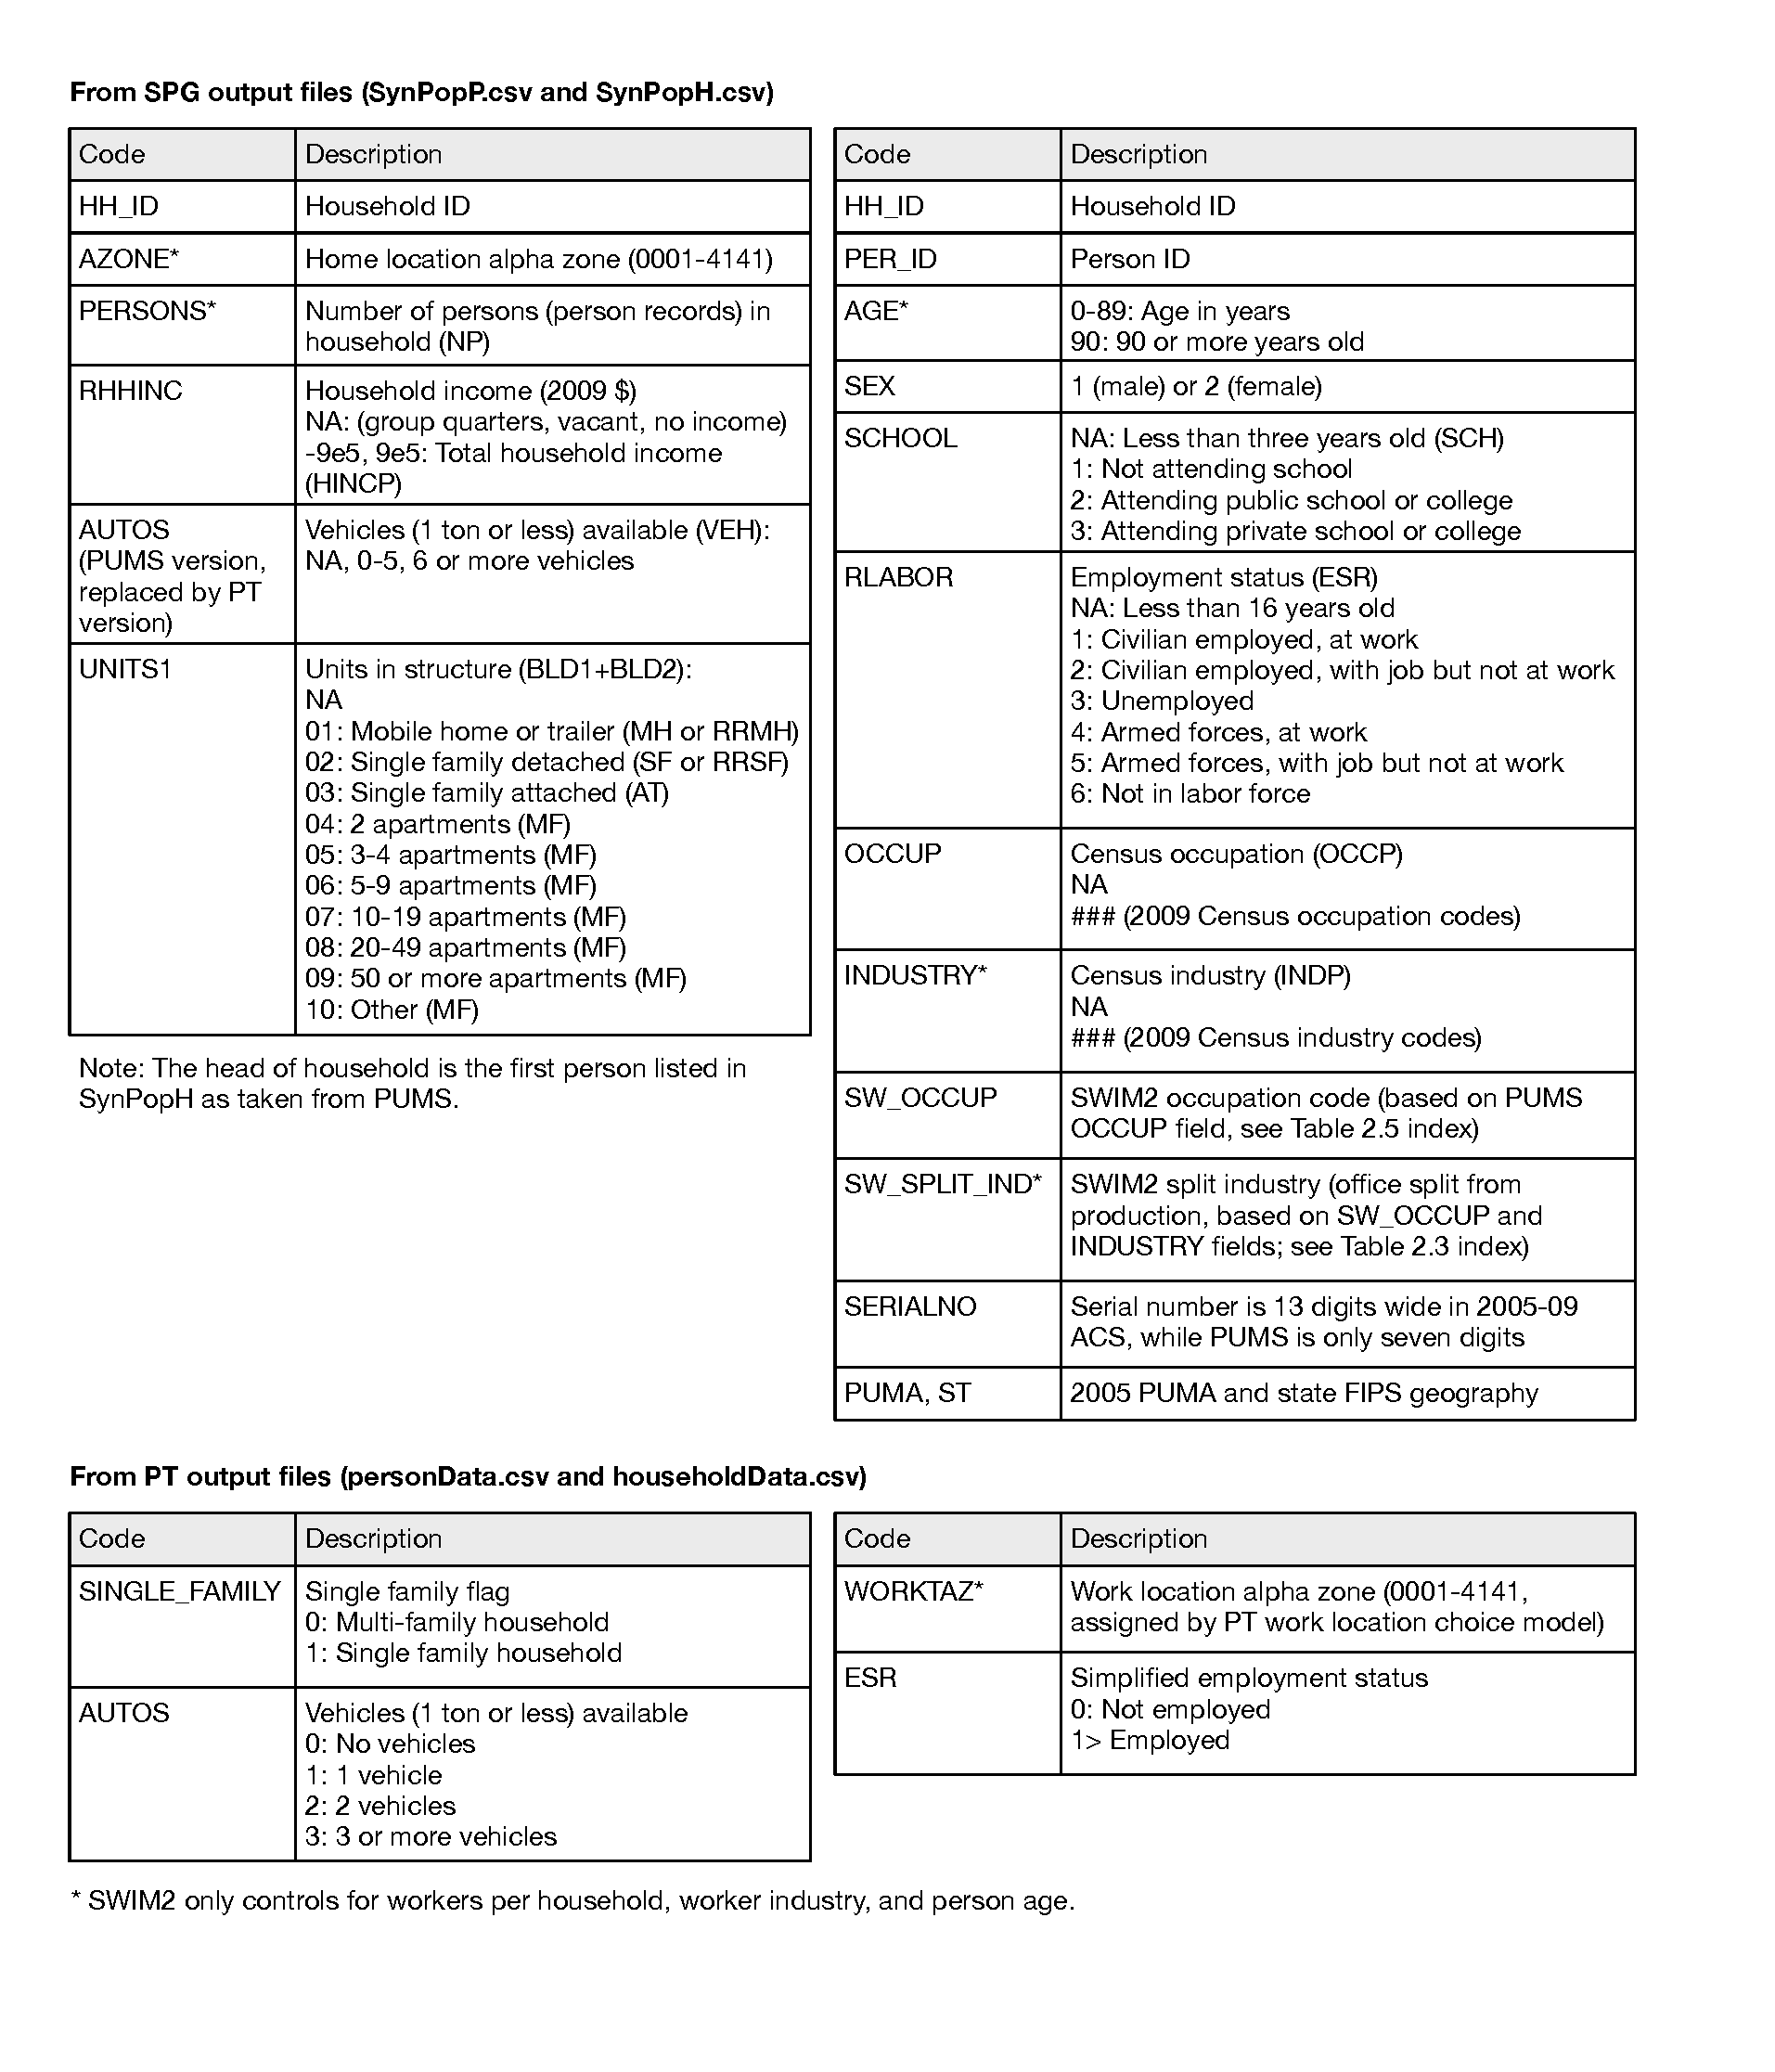
\includegraphics[width=7in]{overview/synthetic-attributes}
\caption{Synthetic population household and person attributes}\label{fig:synthetic-attributes}
\end{figure}

\noindent Other variables that could be retained in the 1990 Census PUMS household record include:
\begin{quote}
SERIALNO, GQINST, ROOMS, TENURE, ACRE10, ONEACRE, YRMOVED, COMMUSE, VALUE, RENT1, MEALS, BEDROOMS, WATER, SEWAGE, YRBUILT, CONDO, AGSALES, RTAXAMT, RFARM, RFAMINC, RWRKR89, RHHFAMTP, RNATADPT, RSTPCHLD, RFAMPERS, RNRLCHLD, RNONREL, R18UNDR, R60OVER, R65OVER, RSUBFAM
\end{quote}

\noindent Other variables that could be retained in the 1990 Census PUMS person record include:
\begin{quote}
SERIALNO, RELAT1, RACE, MARITAL, RSPOUSE, RAGECHLD, YEARSCH, MOBILITY, MILITARY, DISABL1, DISABL2, MOBILLIM, HOURS, WORKLWK, MEANS, RIDERS, DEPART, TRAVTIME, TMPABSNT, LOOKING, AVAIL, YEARWRK, CLASS, WORK89, WEEK89, HOURS89, REARNING, RPINCOME, INCOME1
\end{quote}
 
\section{Running the SWIM2 system}
The SWIM2 system runs on two dedicated computer servers housed at the Transportation Planning Analysis Unit at ODOT. The modeling system is run using a Python script that sets up the directory structure required, calls each of the component modules, and runs the model through time.\footnote{The function was formerly carried out using a model runner system graphical user interface (MrsGUI), which facilitated password-protected remote desktop access to a computing cluster at the State Data Center. MrsGUI executed a series of remote commands required to run the model, to include building scenarios, running the model, providing real-time status information, running post-processing metrics, and transfer of outputs and log files to a local computer.} The SWIM2 User's Guide contains more information on the computing cluster, program installation, file preparation, and instructions for running the model and post-processing scripts. The rest of this section provides an overview of the model directory structure and key functionality of the model runtime process.

All of the SWIM2 components except for the CT module are written in the Java programming language, and makes use of parallel processing where possible to reduce model runtimes. The CT module is written in the R statistical language\footnote{\url{https://www.r-project.org}}, as are some of the post-processing scripts used elsewhere in the model. Finally, the PTV Group's VISUM platform\footnote{\url{http://vision-traffic.ptvgroup.com/en-us/products/ptv-visum/}} is used for highway and transit assignments. It replaces the transport supply (TS) module developed for earlier version of SWIM2. TS was designed to facilitate micro-assignment of trips, whereby the traveler and trip characteristics could be retained through a standard macroscopic traffic assignment. This functionality was no longer needed when it was decided to adopt the aggregate PECAS framework, discussed in Chapter \ref{sec:aa-module-chapter}, in place of evolutionary microsimulated households and firms. Replacing the TS module with VISUM enables faster model runtimes, and reduces the number of modules that the SWIM team must support and maintain.

\subsection{Directory structure}
The directory structure for the SWIM2 system is shown in Figure \ref{fig:directory-structure}. The structure separates user-modified inputs, parameters, base year inputs, from scenario outputs, simplifying the user interface, and facilitating scenario backup and archiving. 

\begin{figure}
\centering
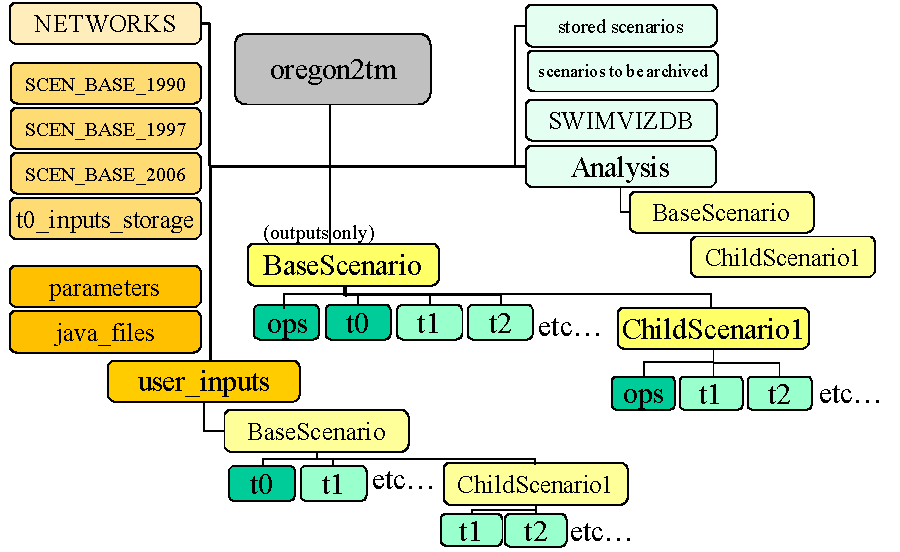
\includegraphics[width=5in]{overview/directory-structure}
\caption{SWIM2 directory structure}
\label{fig:directory-structure}
\end{figure}

After a scenario is created, all input files and code necessary to run the model are split among three folders: parameters (fixed after calibration), java\_files (fixed software and configuration files) and user\_inputs (select set of user-modifiable files). The user\_inputs directory has sub-folders for each scenario and within each folder, a sub-folder for each year. The Analysis folder also has this scenario-year sub-folder structure. A user can set up ``child'' scenarios that hinge off of base or ``parent'' scenarios. Child scenarios, like base scenarios, contain their own year sub-folders that house all child model user\_inputs and outputs (including potential bootstrapped outputs copied in when the child scenario was created). Output scenario-specific log files and the command file used in each run are housed in the scenario's ops folder. This folder structure is described in more detail below.

Each run of the model has its own base scenario directory structure which is a complete reference scenario run and stores full model outputs. Inputs would reside in the user\_inputs, parameters or as the output of other modules, in the current or previous year directory for the scenario. The Base Scenario/t0/ folder files would duplicate the t0\_inputs\_storage folder files, copied into the Base Scenario when created. Child scenarios would simply require the user to create a Child Scenario folder in the user\_inputs folder with appropriate file changes from the base year stored in its scenario-year sub-folders. Running the model would generate the model outputs in the sub-folders of the Base Scenario or Child Scenario.

Some files are constant over time and therefore the modules will always look in the base year t0 directory (or common reference directory) unless directed differently in the properties file. For example, a file of vehicle occupancies used by VISUM that applies to all years would be saved in the t0 VISUM subdirectory. If for vehicle occupancies changed in future year t$n$, for example, a separate file with the new occupancies is placed in the user\_inputs scenario t$n$ subdirectory along with a globalTemplate.properties file (indicating t$n$ path to this file references). This latest occupancy file would then remain in effect until the end of the simulation or until a later year properties file was found. 

\subsection{SWIMVIZ database and visualization tool}
SWIMVIZ was developed to dynamically visualize and inspect core multi-year SWIM2 model results and better understand SWIM2 operations. It contains both a database (SWIMVIZ DB) and an Adobe Flash application tool (SWIMVIZ tool). 

The SWIMVIZ DB conveniently organizes the core output data for all years of a scenario. Data are organized in a few tables at the beta zone level. This standardized format facilitates further output processing using the SWIMVIZ tool or other scripting, such as using SQLite and R statistical software. The key tables are listed in Table \ref{tab:swimviz-key-tables}, with more detail available in the SWIMVIZ DB documentation.

\begin{table}[!t]
\centering
\caption{Key SWIMVIZ database tables created during each model run}\label{tab:swimviz-key-tables}
\begin{tabular}{l L{4.5in}}
\hline
Table & Description \\
\hline
ACTIVITYLOCATIONS & The quantity of activity generated by beta zone, such as industry activity (2009 dollars), households, and employment. \\
\gray BUYSELLMATRIX & The commodity flows from the AA module between beta zones, including the dollar flow of labor, goods and services. \\
EXCHANGERESULTS & Information on the exchange of commodities (goods, services, labor and floorspace), such as the quantity of demand and supply, price, etc. \\
\gray FLR\_INVENTORY & ALD beta zone floorspace inventory and zoning capacity by type. \\
DC\_LOGSUM & Average logsums by beta zone, trip purpose, and market segment. \\
\gray TRIPS\_SDT & Short-distance person trips and trip distances by origin beta zone for each time period. \\
TRIPS\_SDT\_Home & Same as TRIPS\_SDT, except trips are aggregated by person trip household home beta zone origin rather than trip origin. \\
\gray Trips\_LDT & Long-distance person trips and trip distances by origin beta zone for each time period. \\
TRIPS\_LDT\_Home & Same as TRIPS\_LDT, except trips are aggregated by person trip household home beta zone origin rather than trip origin. \\
\gray Trips\_CT & Commercial truck trips and trip distances by origin beta zone and commodity for each time period. \\
TRIPS\_CT\_Home & Same as Trips\_CT, except trips are aggregated by beta zone of truck tour origin, rather than trip origin. \\
\gray TRIPMATRIX & Combined trip matrices for each beta zone origin-destination pair, time period, and mode from SDT, LDT, and CT aggregated to common modes/truck classes. \\
LINK\_DATA & Network assignment results (volumes, etc.) for each time period. \\
\gray SKIM & Travel distance, time, tolls for each beta zone origin-destination pair for peak and off-peak, auto and truck. \\ 
MODELWIDE & Various modelwide data, typically associated with the NED module. \\
\hline
\end{tabular}
\end{table}

A SWIMVIZ Micro database stores the synthetic population (persons and households from SPG), as well as detailed tour and trip information for person (from PT) and trucks (from CT). The key tables included in this database are shown in Table \ref{tab:swimvia-micro-tables}, with more detail available in the SWIMVIZ DB micro documentation and SWIM2 User's Guide.

\begin{table}
\centering
\caption{Key SWIMVIZ microdata tables created during each model run}\label{tab:swimvia-micro-tables}
\begin{tabular}{l L{4.8in}}
\hline
Table & Description \\
\hline
HH & Households in the model and their key attributes, including description of any long distance tours. \\
\gray PER & Persons in the model and their key attributes, including industry, work status. \\
TOUR\_LDT\_MICRO & All long distance tours in the model, including their purpose, mode origin and destination zones, times and party size. \\
\gray TRIP\_LDT\_MICRO & All long distance vehicle trips in the model, including their purpose, mode origin and destination zones and times. \\
TOUR\_SDT\_MICRO & All short distance tours in the model, including their purpose, mode origin and destination zones and times. \\
\gray TRIP\_SDT\_MICRO & All short distance person trips in the model, including their purpose, mode origin and destination zones and times. \\
TRIP\_CT\_MICRO & All short and long distance truck trips in the model, including commodity, carrier type, weight origin and destination zones and times. \\
\hline
\end{tabular}
\end{table}

During model setup the user can flag that a scenario produce one or both of these VIZ DBs. Then a SQLite database for each year of the scenario is created after the model run completes and compiled into a master scenario sqlite database that contains all years. A zipped version of the multi-year SWIMVIZ DB is copied to the ODOT FTP site facilitating remote users in obtaining this data.

\subsection{Application Orchestrator (AO) component}
The AO module is a collection of components that directs the flow of the full SWIM2 Model. The key components of AO include:
\begin{itemize}
\item The Distributed Application Framework (DAF)
\item Launching components (using Ant and ApplicationOrchestrator.java and FileMonitor.java)
\item Monitoring progress (using Logger.java)
\end{itemize}

\noindent The SWIM2 components are either monolithic and distributed. A monolithic application is one that is run on a single machine, more specifically inside a single Java Virtual Machine (JVM), also referred to as a node. The NED, ALD, AA, SPG1, and SPG2 components are monolithic. A distributed application is one that is run on multiple machines or inside several JVMs, or in other words on more than one node. A collection of nodes that communicate with one another is called a cluster. PT and CT are examples of distributed applications. These applications could be run monolithically, but distributing the process over multiple nodes significantly decreases their run times. The code is broken up into tasks that can be performed simultaneously on different nodes for a different set of objects. For example, a task might calculate the composite buying and selling utilities for each commodity. If distributes across eight nodes, for example, the composite utilities can be calculated in parallel. There is some coordination required when separating code into tasks, as the data has to once again be combined. The Distributed Applications Framework Version 2 (DAF2) provides this coordination. The CT component uses the doParallel package in the R statistical language to achieve the same effect.

The DAF code was written to handle the distribution of an application over multiple nodes. It provides the communication mechanism, a messaging system, that allows the nodes to send messages to tasks on other nodes, receive messages and to listen for messages from other nodes. Tasks listen for messages to arrive in a work queue associated with that task. As soon as work arrives it is processed, and a return message is usually sent. DAF also provides methods to start and stop all nodes in a cluster from a single node and to start an application from a node outside of the cluster. 

A daf.properties file is used to define a DAF cluster. A cluster can be a single machine that runs multiple JVMs with one task per JVM, or perhaps five machines running five JVMs with ten tasks running in each JVM. Machine memory is the biggest constraint, as each JVM uses up to 8 gigabytes (GB) or more of memory. The daf.properties file describes only the nodes, and therefore the cluster is defined independent of the application that will be run on it. An application may utilize all nodes in a cluster or only a subset of them. An application-specific daf.properties file is therefore also necessary to describe each task that the application will perform and assign it to a particular node. The work queues are defined in the properties file where they are associated with a particular task and a particular node. MrsGUI codifies various set DAF configurations.

The structure of a DAF application is illustrated in Figure \ref{fig:daf-example}. It shows how a component might be distributed over three nodes. For the example described above the tasks might include a master task, a CUWork task (calculating the composite utilities of buying and selling a particular commodity in a particular exchange zone), a SDWork task (calculating the surplus and its derivative of a particular commodity in a particular exchange zone), two result processing tasks, and associated work queues.

\begin{figure}
\centering
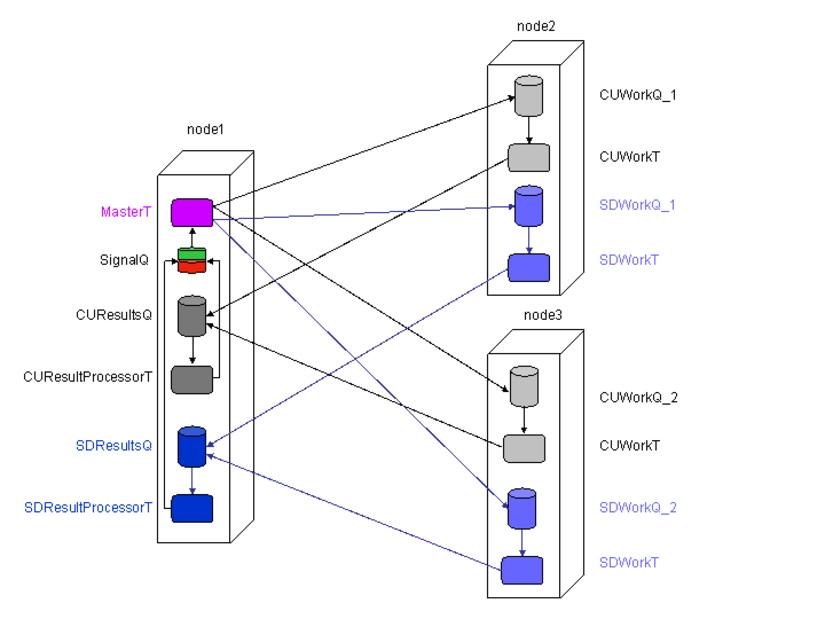
\includegraphics[width=5in]{overview/distributing-pi-module}
\caption{Distributing component flows}
\label{fig:daf-example}
\end{figure}

\subsection{Launching a component}
The launch of each component is currently being done using Python ANT Substitute (PANTS), a program which was created to replace the previous component launching program, Ant. One of the benefits of PANTS are that it allows tasks to be specified in Python (as opposed to XML, which is used by Ant), which allows a natural program flow to be specified using standard programming idioms. Another advantage is that it stores an entire run sequence in a database, which allows the model run's sequence position to be determined, as well as allowing a run to be continued if it was stopped. PANTS uses a definition file written in Python, which specifies targets which are accessible to the user. These targets build up a model sequence, which is then loaded into a database and finally the sequence is executed using database queries to determine each step

In the case of the monolithic components the PANTS target (e.g., runED, runALD) located in the TlumipDef.py file starts a new JVM on a machine in the cluster, instantiates the AO object inside it, and passes to it the name of the component (e.g., NED) to be started. AO then simply creates an instance of the named component and calls its runModel method. This assumes that the constructor of that component will read the appropriate properties file and configuration files. Properties files contain runtime information, such as the name of input files. Configuration files hold the things that do not change, such as internal parameter values. The component will then handle the rest of the processing. Each module component will clean up after their run and communicate with other components via data files and thus, does not return data structures or other information to the orchestrator. 

A distributed component is also launched using a PANTS target so that the AO is created inside its own node, as discussed above. For the distributed components, however, this node must start other nodes both on its local machine as well as nodes on remote machines in the cluster. A FileMonitor object is the mechanism by which the Orchestrator object communicates with DAF. The FileMonitor class uses a simple text file as a command file, and serves as a central command station. Each machine in a DAF cluster will create a FileMonitor object in a small JVM. This object monitors the command file for changes. When a change in the lastDateModified attribute is detected, the FileMonitor reads the contents of the file and executes the command found therein. 

Thus, to start a distributed application, the AO object first writes StartNode into the command file. AO waits for a short time and then writes ``StartCluster'' into the command file, overwriting the previous command. The orchestrator again waits and then writes the name of the application that is supposed to run into the command file. The FileMonitors, detecting the changes, execute the appropriate code on their machine. AO then waits for the appearance of a ``done'' file that will be written by the application when it has finished executing. When the done file appears, AO will write ``StopNode'' into the command file and the FileMonitors will stop the Java processes running on the machines.

%For more information on the FileMonitor class, see additional reference on this topic [3]. 

\subsection{Logging}

AO uses logging statements generated by the individual modules to provide feedback to the users as to the module's progress. These log statements can be directed to the console or to a file as specified in a logging.properties that is shared by all components. The following logging output is generated automatically and written to the Scenario /ops directory during a model run:
\begin{itemize}
\item Main\_event.log (the main process log file)
\item Node[node number]\_event.log (the log file for the DAF node on computer [node number])
\item Bootstrap\_server\_node[node number].log, bootstrap\_client.log, fileMonitor\_event.log (logs related to the inner workings of the DAF components)
\item Global\_status.log (a global status log file)
\item Status.log (a module-level status log file)
\end{itemize}

\noindent In addition to the log files, at the end of each run, a Java program is run which reads the log files and summarizes the run at both a global and module level. The files created by the process (also placed in the /ops directory) include ModuleSummary.csv (an overall summary of the runtimes of the various modules) and PtIterationSummary.txt (a summary of the PT module). 
 
\section{Calibration approach}\label{sec:calibration-approach}
A three-stage process is used to develop the values for the parameters in the various modules in the model:
\begin{itemize}
\item In Stage 1 (\textbf{S1}) values are developed for certain parameters in each module separately. The intention is that these first-stage values for the S1 parameters will remain fixed as the model development and calibration work progresses. When suitable observations of system behavior are available, statistical methods are used to estimate appropriate values for S1 parameters. In some cases, only a single observation is available and direct methods are used to provide values. At this point it is not necessary that the modules can be run: the components of the modules are being ``assembled'' and the outputs of the modules are not yet being considered.
\item In Stage 2 (\textbf{S2}) initial values are established for all of the parameters that are not S1 parameters, considering the fit of each module in isolation. The fit for a given module concerns specified targets for outputs from the module, so the module needs to be run in order for it to provide these outputs. Thus, a full set of required inputs for each module needs to be developed, including all those provided by other modules and all those provided exogenously. In order to obtain reasonable values for the S2 parameters, these inputs need to be consistent with the specified targets, representing conditions similar to those that gave rise to the targets.
\item In Stage 3 (\textbf{S3}) the initial values established for certain sets of the S2 parameters are revisited for all of the modules simultaneously, considering the fit of all modules together. These are evaluated with the full model running, so that inputs to the modules are coming from the other modules in the way they would for a model run. The second and third stages together constitute a Bayesian updating process for these S3 parameters. Ideally, all parameter values would be revisited, but this is not possible for practical reasons. A weight sensitivity matrix can be used to explore the remaining lack-of-fit for the entire model, which can help identify the parameters to focus on in the third stage and which may lead to small changes in the details of the model design and specification.
\end{itemize}

The development of the values for the S1 and S2 parameters, in the first and second stage of the parameter development process, is described for each module in the subsequent chapters. This includes a description of the work done to get each module running, as required, using input values and certain interim values for parameters as required. 

Certain initial values for the S2 parameters are revisited in Stage 3 of the parameter development process. Stage 3 includes the work necessary to get the entire set of all SWIM2 components running in order to provide a fully integrated modeling system. All SWIM2 components, excluding the optional selected link (SL) component, have completed this three-step calibration process.

\chapter{New economic and demographic (NED) component}\label{sec:ned-chapter}
The New Economics and Demographics (NED) Module replaces the original Economics and Demographics (ED) module. The initial ED module provided annual predictions of industry activity (output) for the PI module (now replaced with the AA module), employment for the SPG module, and final demand by aggregated industry category for Oregon and scaled those to the full model area using fixed factors. The ED module also reported region-wide construction activity dollars to the ALD module. The demographic portions of the ED module were not used by other modules in the Oregon Statewide Integrated Model. An optional EPF module (no longer used) modified the ED outputs in response to PI model-wide industry location utility trends.

The ED module produced forecasts that were internally consistent, but not necessarily consistent with forecasts from any other model. As a result, a lot of effort went into overriding ED forecasts to develop reference scenarios that were consistent with official state forecasts, which changed every quarter.

The NED module is organized around the concept of scenarios. A scenario is a complete set of NED output that is intended to represent the economic and demographic aspects of a particular future to be modeled. NED outputs are all at the model-region-wide level include forecast output and employment by AA activity, imports and exports by AA commodity, and population by five-year age category. Construction activity and government investment forecasts are reported separately as well. All units are in 2009 dollars, consistent with the rest of SWIM2.

The NED module has three main components:
\begin{enumerate}
\item An exogenously-defined reference scenario that is consistent with assumptions that drive ongoing planning efforts in Oregon.
\item An optional feedback mechanism that allows transportation and land-use policy changes to drive deviations from the way a scenario would progress over time under the policy assumptions that underlie the reference scenario.
\item A scenario generator to allow the definition of alternative economic scenarios to be evaluated
The NED module does not include an economic or demographic model of its own. It consists instead of a representation of the output from exogenous economic and demographic models and the ability to modify those values in appropriate and consistent ways in response to deviations from the reference case in the scenario being evaluated.
\end{enumerate}

A proposed Economic Feedback model (if used) will allow prior year AA modelwide industry location utility trends among other factors to influence NED forecasts, prior to use by other modules. Other NED outputs could also be used to improve consistency and scenario policies, such as SPG to use as constraints the unemployment rate and absolute (rather than distributions of) population by age. 

\section{Theoretical basis}
The change in thinking that led to the replacement of the economics and demographics module (ED) also removed the theoretical basis for having an independent macroeconomic model within SWIM. There remain theoretical bases for the feedback and scenario generation components of NED. 

Feedback modifies current-year NED output in response to deviations from reference-scenario levels in prior year(s) output from other model components. The feedback module operates using elasticities, which define a fixed, linear relationship between proportional change in another module's output and proportional change in a NED quantity. Economic demand and supply functions are almost never linear, but do tend to exhibit fairly constant elasticities, especially over observed ranges of price and quantity. One drawback to relying on elasticities is that when one quantity goes to zero, the other becomes undefined.

If a variable to be fed back is a logsum, it is important that the elasticity to be applied be estimated from logsum data produced using all the same logit-model coefficients that produced the logsum being fed back. Logsum values have no absolute meaning; they have meaning only in relation to other logsums produced from the same logit-model coefficients.

The elasticity parameters to be used in the feedback mechanisms have not yet been estimated. They will be estimated from empirical data and validated against theoretical expectations for their sign and magnitude.

Scenario generation modifies reference-case NED output in future years in advance of running the model based on specifications supplied by the analyst running the model. There is no necessary theoretical basis for the scenarios to be evaluated, but there is a theoretical basis for the translation from the changes in policy variables that the user will have control over and the internal NED variables that the scenario generator will change. The mechanism for translation, which has not yet been implemented, will rely on parameters estimated from empirical data, including input-output model data, and validated against theoretical expectations for their sign and relative magnitude.

\section{Quantity definitions and categories}
NED operates exclusively at the modelwide level. NED produces estimates of employment and output by unsplit AA activity, of imports and exports by commodity\footnote{See the definition of commodities used in the model in Table \ref{tab:goods-categories} on page \pageref{tab:goods-categories}.}, of residential and non-residential construction activity, and of government investment in three categories (federal, state, and capital government accounts). The unsplit AA activity set noted below are further disaggregated by space usage (heavy/light industries and office/non-office) in AA to arrive at the full AA activities noted earlier in Table \ref{tab:activity-industry} (page \pageref{tab:activity-industry}).

\section{Component models}

The NED model involves the following components, described in more detail in the remainder of this section:
\begin{itemize}
\item Reference scenario (exogenously-defined)
\item Feedback mechanism (optional) 
\item Scenario generator (optional)
\end{itemize}
\noindent Each of these are discussed in the following sections.

\subsection{Reference scenario}
The reference scenario is built from external data and forecasts. It starts with IMPLAN data for the model region for 2009 for output, employment, imports, exports, and population. IMPLAN populations are subdivided into five-year age groups using Census data. The 2009 data is kept separate for Oregon and for each of the portions of Washington, Idaho, Nevada, and California that are in the halo. 

\subsubsection{Employment forecasts}
The software implementation of the reference scenario generator allows for separate employment forecasts for each state and a national forecast that substitutes for state forecasts in years for which state forecasts are not available. Oregon provides an official forecast that goes out at least eight years. None of the halo states provide official forecasts more than two years out. Employment growth rates from the Oregon forecast currently are used for all states for the years for which they are available, and then employment growth rates from the national forecast are used. We expect that the actual growth rates in the halo region will more closely resemble Oregon's than the rest of the nation. The national forecast is produced by Global Insight and purchased by the State of Oregon to drive its own forecasting models, including the state forecast we use of Oregon. We therefore expect that the Oregon forecast and the national forecast will be consistent with each other.

Employment is forecast by IMPLAN sector (440 sectors) using a crosswalk that matches one exogenous forecast sector to each IMPLAN sector. Exogenous forecasts have many fewer sectors than IMPLAN and each has its own set of sectors and its own crosswalk. Each year's employment in each IMPLAN sector is forecasted by applying the ratio of that year's employment to the prior year's employment in the corresponding sector in the exogenous forecast to the prior year's employment in that IMPLAN sector.

Employment by state within the model region is aggregated over all states for each IMPLAN sector. Employment by IMPLAN sector is then aggregated to employment by AA activity (52 activities) using a crosswalk that allows IMPLAN sectors to be split among AA activities if necessary. 

\subsubsection{Output forecasts}
For each sector in the national forecast, the ratio of labor productivity (output per employee) in the current year to labor productivity in the prior year is calculated. For each IMPLAN sector in the employment forecast, the minimum of this ratio or 1.05 is applied to the prior years labor productivity within the model region and the resulting, updated labor productivity is multiplied by the forecast of employment for the current year in the model region, yielding forecasted output for that IMPLAN sector in the model region in the current year. 
Output by IMPLAN sector is then aggregated to output by AA activity (52 activities) using a crosswalk that allows IMPLAN sectors to be split among AA activities if necessary. The splits may be different for output than for employment.

\subsubsection{Trade forecasts}
For each IMPLAN sector, the ratio of the current year's output to the base year's output is calculated. Each industry's make of each export commodity from the base-year IMPLAN structural matrices is then scaled by that sector's ratio to get exports by that industry. Each industry's use of each import commodity from the base-year IMPLAN structural matrices is scaled by that sector's ratio to get imports by that industry.

The ratio of current-year population to base-year population is calculated and applied to institutional imports and exports by commodity from the base-year IMPLAN structural matrices to get current year imports and exports by institutions.

Industry and institution imports and exports are aggregated by IMPALN commodity (440 commodities) and then aggregated to AA commodities (52 commodities) using a crosswalk that allows IMPLAN commodities to be split among AA commodities if necessary.

\subsubsection{Construction forecasts}
Construction forecasts are a re-arrangement of the construction output dollars into residential and non-residential structures construction dollars and the exclusion of other non-residential construction activity, such as road building.

\subsubsection{Government forecasts}
Government forecasts use elasticities of government revenue with respect to total employment to estimate state and local government revenue, federal revenues from corporate taxes, and federal revenues from other taxes.

\section{Software implementation}
The NED module and its sub-components are implemented in the Java programming language, and uses Python scripts to execute most NED functions.

\subsection{Reference scenario}
The software implementation of the NED module is a Python script. Each time it is run, it is given a pointer to a parameters file, which it reads to obtain the following parameters:
\begin{itemize}
\item ned.input.directory (where baseline scenario files are read from)
\item ned.activity\_forecast.path (where model-year activity forecast is written)
\item ned.trade\_forecast.path (where model-year trade forecast is written)
\item ned.construction\_forecast.path (where model-year trade forecast is written)
\item ned.population\_forecast.path (where model-year population forecast is written)
\item ned.government\_forecast.path (where model-year government forecast is written)
\item ned.prior\_activity\_forecast.path (where prior-year activity forecast is read from)
\item ned.prior\_trade\_forecast.path (where prior-year trade forecast is read from)
\item ned.prior\_construction\_forecast.path (where prior-year construction forecast is read from)
\item ned.prior\_population\_forecast.path (where prior-year population forecast is read from)
\item ned.prior\_government\_forecast.path (where prior-year government forecast is read from)
\item ned.base.year (e.g., 2009)
\item ned.model.year (an integer value; not a calendar year)
\item ned.base.year.model.year (the model year identifier for the base year)
\item ned.allow.feedback (currently always false)
\end{itemize}

\noindent In the base year, the NED module reads values for that year from the Baseline Scenario files and writes them to that year's NED model files. In subsequent model years, it reads that year's and the prior year's baseline forecast from the Baseline Scenario files, the prior year's model-run forecast, and the prior-year values of feedback variables from other modules.

For each variable in each forecast, the NED module calculates the ratio of this year's value to last year's in the Baseline Scenario. If feedback is enabled, it then adjusts those ratios using the fed-back values from other modules.\footnote{This adjustment is not yet implemented because the variables to be fed back and the elasticities relating change in fed-back variables to changes in NED variables have not yet been identified.} If feedback is not enabled (as is currently always the case), the adjustment factor is 1.0.

The NED module then applies the adjusted ratios to its prior-year forecast to obtain the model-year forecast. The model-year forecasts are then written to the appropriate directories.

Files that NED generates for other modules are written to the appropriate directories as specified in the ned.*\_forecast.path parameters. However, the baseline forecast data that NED uses over time resides in a single directory, specified by the ned.input.directory parameter. The files in that directory are in the same format as the output files except that they have an extra column on the left, in which the year is specified. All NED inputs and outputs represent the entire model region (including Oregon and the halo) and all dollar values are in 2009 dollars.

\subsection{Baseline scenario generator}
The NED Baseline Scenario Generator runs outside of the SWIM2 modeling framework and produces the NED input files that must exist before the SWIM2 model is run. It gathers data from several IMPLAN output files, from state economic forecast files, from the Global Insight national long-run economic forecast files, and from files containing crosswalks and sector mappings. The IMPLAN and forecast files are in their original format, so the Baseline Scenario can be updated by substituting newer copies of the forecast files and then rerunning the Baseline Scenario Generator, without any need to modify the new forecast files. Significant changes in the format of the forecast files by the entity that produces them would require either modifying the code or reformatting the input file. In anticipation of likely changes to forecast files (such as dropping historical years), the code uses named constants to make adjusting the code easy (e.g., a named constant to identify the column in which base-year data are found).

The scenario starts by building internal data structures to hold input values and the results of intermediate calculations. It then reads from various input files and puts their data into the internal data structures. 

Base year results for the Baseline Scenario are calculated by aggregating IMPLAN data to the categories used in SWIM2. IMPLAN population for the model region is attributed to five-year age groups based on 2010 census data proportions. Each subsequent year is then forecasted by applying the appropriate growth rate from each state's forecast to the prior year's employment within that state. If there is no forecast for that state, or if the model year is beyond the end of the state's forecast, the appropriate growth rate from the national forecast is used. Employment is then aggregated over IMPLAN sectors to SWIM2 categories and over states to model region totals.

The states do not forecast output. To forecast output, the ratios of output per employee in each sector in the current year to that in the prior year from the national model is calculated and applied to the prior year's output per employee for the region. The adjusted output per employee is then multiplied by forecasted employment to obtain a forecast of output.

Population in forecasted by applying growth rates by five-year age group from the Oregon population forecast to the prior year's model region population. We do not have population forecasts specific to the halo portions of neighboring states, and assumed that population growth in those counties would be more similar to that in Oregon than to the rest of their states or the nation.

For the trade forecast, industry imports and exports are forecasted separately from institution imports and exports. Industry exports are forecasted by taking the ratio of output for each industry in the model year and the base year and applying it to the exports of each commodity made by that industry in the base year. Industry imports are forecasted by taking the ratio of output for each industry in the model year and the base year and applying it to the imports of each commodity used by that industry in the base year. Imports and exports by institutions (e.g., households and governments) are calculated similarly, but using population ratios rather than output ratios.

The construction forecast used by ALD is constructed by aggregating output dollars from IMPLAN construction sectors.

The government forecast uses estimated elasticities relating change in government revenues to change in employment, which are applied to the change in forecasted employment to get change in government revenue, which is then applied to the prior year's government. The estimated elasticities used are stored in named constants near the top of the script. 

\section{S1 and S2 module parameters}\label{sec:ned-s1-s2}

NED as currently implemented is primarily an exogenous forecast. As such, the Reference Scenario has no estimated parameters, and makes just a few assumptions noted below. In the future the to-be-developed NED Feedback and Scenario Generator model will increase the number of parameters and assumptions. 

The estimated elasticities used in the Reference Scenario government forecast are:
\begin{itemize}
\item FED\_TAX\_ELASTICITY = 1.214
\item SL\_TAX\_ELASTICITY = 1.234
\item CORP\_TAX\_ELASTICITY = 1.054
\end{itemize}

\section{Inputs and Outputs}

The NED input data needed to integrate with the full SWIM2 model components are listed in Table \ref{tab:ned-inputs}. The Reference Scenario as noted was developed from source forecasts, particularly the Oregon OEA forecast and the national Global Insight forecast, along with IMPLAN relationships to disaggregate within Oregon and expand to other states in the halo region of the model. To build this key NED reference scenario input requires the source file datasets listed in Table \ref{tab:ned-source-files}. NED outputs that are used by other parts of SWIM2 are shown in Table \ref{tab:ned-outputs}. NED monetary outputs used by other modules --- AA activity dollars and ALD construction dollars --- are in units of year 2009 dollars, consistent with the rest of the SWIM2 model. 

\begin{table}  % Table 3-1
\centering
\caption{Required inputs for NED}\label{tab:ned-inputs}
\begin{tabular}{L{1.8in} L{3.2in} L{0.85in}}
\hline
Data element & File(s) & Source \\
\hline
Reference scenario forecasts for all years & activity\_forecast.csv, trade\_forecast.csv, government\_forecast.csv, construction\_forecast.csv, population\_forecast.csv & Exogenous \\
\gray Modelwide composite utilities of production activity & ActivitySummary.csv & AA (future) \\
\hline
\end{tabular}
\end{table}

\begin{table}  % Table 3-6 (apparently tables 3-2 through 3-5 never defined)
\centering
\caption{NED source files for the Reference Scenario}\label{tab:ned-source-files}
\begin{tabular}{ll}
\hline
Input file & Data structure \\
\hline
Oregon Industry Detail.xls & implan\_activity \\
\gray Washington Industry Detail.xls & implan\_activity \\
Idaho Industry Detail.xls & implan\_activity \\
\gray Nevada Industry Detail.xls	 & implan\_activity \\
California Industry Detail.xls & implan\_activity \\
\gray OregonAndHalo Industry Detail.xls & implan\_activity \\
cge\_IxI.csv & implan\_structure \\
\gray employment\_annual.xls & state\_forecasts \\
pop\_forecast.xls & population \\
\gray Baseline LR Growth Scenario 2011\_05.xls & national\_forecast \\
implan\_ned\_activity.xls & implan\_ned\_activity \\
\gray implan\_aa\_commodity.xls & implan\_aa\_commodity \\
IMPLAN\_OEA.xls & state\_crosswalks \\
\gray implan\_gi\_sectors.xls & state\_crosswalks \\
\hline
\end{tabular}
\end{table}

\begin{table}
\centering
\caption{NED outputs used by other SWIM2 modules}\label{tab:ned-outputs}
\begin{tabular}{L{3.9in} L{1.6in} L{0.5in}}
\hline
Description & File(s) & Users \\
\hline
Count of modelwide workers by SPG industry & activity\_forecast.csv & SPG1 \\
\gray Modelwide residential and nonresidential final demand of new construction dollars & construction\_forecast.csv & ALD \\
Modelwide quantities of production activity (dollar flows) by AA industry/institution & activity\_forecast.csv, government\_forecast.csv & AA \\
\gray Modelwide quantities of import/export activity (dollar flows) by AA commodity-specific activities & trade\_forecast.csv & AA \\
\hline
\end{tabular}
\end{table}

\section{Validation} 
ED can be compared to the OEA forecast to validate that it is replicating this key source data. Because of the way the reference scenario is built, the rate of employment growth in each sector in the reference scenario is identical to the rate of employment growth in the comparable sector in the OEA employment forecast through the last year of the OEA forecast. 

The following tables show the Reference Scenario quantities and their base-year (2009) values for the model region. This includes employment and output (Table \ref{tab:ned-employment-output}) and population (Table \ref{tab:ned-population-output}) used by SPG. It also includes government accounts (Table \ref{tab:ned-government-accounts}) and trade activity (Table \ref{tab:ned-trade-activity}) used by AA. It also included \$7.89 billion in residential construction and \$7.63 billion in non-residential construction.

\begin{sidewaystable}
\centering
\caption{Model region employment and industry output in the reference scenario base year (2009)}\label{tab:ned-employment-output}
\small
\begin{tabular}{lrr|lrr}
\hline
Activity & Employment & Output & Activity & Employment & Output \\
\hline
CNST\_main\_xxx  & 22,876 & 3,690,346,435 & MFG\_htec\_hi  & 3,634 & 13,063,887,807 \\
\gray CNST\_nRES\_xxx  & 40,908 & 6,542,617,309 & MFG\_htec\_li  & 3,335 & 13,063,887,807 \\
CNST\_offc\_off  & 72,450 & 0 & MFG\_hvtw\_hi  & 22,842 & 14,441,531,006 \\
\gray CNST\_othr\_xxx  & 49,796 & 8,729,001,953 & MFG\_hvtw\_li  & 23,038 & 14,441,531,006 \\
CNST\_RES\_xxx  & 27,477 & 6,740,919,189 & MFG\_lvtw\_hi & 11,756 & 12,978,764,067 \\
\gray ENGY\_elec\_hi  & 5,131 & 8,621,276,855 & MFG\_offc\_off  & 147,103 & 0 \\
ENGY\_ngas\_hi  & 880 & 3,603,145,996 & MFG\_wdppr\_hi  & 25,917 & 11,847,955,596 \\
\gray ENGY\_offc\_off  & 24,548 & 0 & RES\_agmin\_ag  & 98,434 & 16,903,898,303 \\
ENGY\_ptrl\_hi  & 8,672 & 4,631,318,359 & RES\_forst\_log  & 8,356 & 2,519,144,897 \\
\gray ENT\_ENT\_RET & 79,100 & 3,571,715,370 & RES\_offc\_off  & 62,525 & 0 \\
FIRE\_fnin\_off  & 150,334 & 31,902,799,194 & RET\_auto\_RET & 99,235 & 7,439,574,272 \\
\gray FIRE\_real\_off  & 139,465 & 15,446,998,046 & RET\_nstor\_off  & 46,075 & 2,193,797,363 \\
GOV\_admn\_GOV & 101,916 & 19,036,836,853 & RET\_stor\_off  & 56,858 & 0 \\
\gray GOV\_offc\_off  & 162,605 & 0 & RET\_stor\_RET & 229,125 & 16,026,845,092 \\
HIED\_hied\_off\_inst  & 80,247 & 4,569,757,377 & SERV\_bus\_off  & 172,808 & 14,387,504,547 \\
\gray HLTH\_care\_inst  & 68,190 & 3,849,533,203 & SERV\_home\_xxx  & 54,899 & 456,867,797 \\
HLTH\_HOSP\_HOSP & 88,618 & 12,295,007,812 & SERV\_nonp\_off\_inst  & 132,924 & 9,376,816,406 \\
\gray HLTH\_othr\_off\_li  & 150,943 & 18,144,155,090 & SERV\_site\_li & 66,752 & 5,828,886,779 \\
HOSP\_acc\_acc  & 35,825 & 3,539,955,230 & SERV\_stor\_RET & 80,595 & 5,164,732,788 \\
\gray HOSP\_eat\_RET\_acc  & 219,159 & 12,374,280,273 & SERV\_tech\_off  & 219,305 & 22,817,588,607 \\
INFO\_INFO\_off  & 48,211 & 0 & TRNS\_TRNS\_off  & 45,284 & 0 \\
\gray INFO\_INFO\_off\_li  & 9,848 & 15,239,006,202 & TRNS\_TRNS\_ware  & 66,544 & 14,723,200,435 \\
K12\_K12\_K12 & 167,668 & 12,626,084,053 & UTL\_othr\_off  & 14,870 & 0 \\
\gray K12\_K12\_off  & 57,305 & 0 & UTL\_othr\_off\_li  & 17,928 & 8,378,148,941 \\
MFG\_food\_hi  & 14,999 & 10,829,728,776 & WHSL\_offc\_off  & 27,646 & 0 \\
\gray MFG\_food\_li  & 15,124 & 10,829,728,776 & WHSL\_WHSL\_ware & 86,026 & 19,829,592,529 \\
\hline
\end{tabular}
\end{sidewaystable}

\begin{table}
\centering
\caption{Model region population by age in the reference scenario base year (2009)}\label{tab:ned-population-output}
\begin{tabular}{cr|cr}
\hline
Age group & Population & Age group & Population \\
\hline
0 to 4 & 448,259 & 45 to 49 & 451,390 \\
\gray 5 to 9 & 437,565 & 50 to 54 & 457,376 \\
10 to 14 & 449,472 & 55 to 59 & 444,001 \\
\gray 15 to 19 & 465,230 & 60 to 64 & 397,944 \\\
20 to 24 & 463,974 & 65 to 69 & 226,955 \\
\gray 25 to 29 & 456,518 & 70 to 74 & 185,181 \\
30 to 34 & 450,878 & 75 to 79 & 160,906 \\
\gray 35 to 39 & 448,466 & 80 to 84 & 143,361 \\
40 to 44 & 448,611 & 85+ & 120,209 \\
\hline
\end{tabular}
\end{table}

\begin{table}
\centering
\caption{Government accounts for the reference scenario base year (2009)}\label{tab:ned-government-accounts}
\begin{tabular}{lr}
\hline
Government category & Value (2009 \$) \\
\hline
Federal government (FGOV\_acct\_gov) & 93,817,953,918 \\
\gray State and local government (SLGOV\_acct\_gov) & 71,879,103,322 \\
Capitol expenditures (CAP\_acct\_gov) & 69,549,704,567 \\
\hline
\end{tabular}
\end{table}

% Trade activity by commodity monster table (3-10)
\begin{footnotesize}
\begin{longtable}{lr|lr}
\caption{\normalsize{Trade activity by commodity for the reference year base scenario (2009)}}\vspace{-9pt} \\
\hline
Trade activity & Value (2009 \$) & Trade activity & Value (2009 \$) \\ \hline
\endfirsthead
\hline
Trade activity & Value (2009 \$) & Trade activity & Value (2009 \$) \\ \hline
\endhead
\hline \multicolumn{4}{r}{\emph{Continued on next page}}
\endfoot
\hline
\endlastfoot\label{tab:ned-trade-activity}
accommodations\_expt & 3,270,897,187 & sctg17\_pcc\_fuel\_expt & 21,714,405 \\
\gray accommodations\_impt & 2,541,892,752 & sctg17\_pcc\_fuel\_impt & 5,642,668,465 \\
communications and utilities\_expt & 5,678,834,996 & sctg18\_pcc\_petr\_oil\_expt & 10,857,202 \\
\gray communications and utilities\_impt & 7,869,734,616 & sctg18\_pcc\_petr\_oil\_impt & 2,821,334,232 \\
construction\_expt & 9,180,101,387 & sctg19\_pcc\_coal\_prod\_expt & 200,319,354 \\
\gray construction\_impt & 12,590,735,942 & sctg19\_pcc\_coal\_prod\_impt & 4,069,050,714 \\
education reports to sponsors\_expt & 104,924,774 & sctg20\_pcc\_chem\_basic\_expt & 1,126,536,613 \\
\gray education reports to sponsors\_impt & 37,468,124 & sctg20\_pcc\_chem\_basic\_impt & 1,891,511,255 \\
energy\_expt & 3,123,152,392 & sctg21\_pcc\_chem\_pharma\_expt & 764,919,598 \\
\gray energy\_impt & 1,143,833,082 & sctg21\_pcc\_chem\_pharma\_impt & 6,235,158,377 \\
entertainment services\_expt & 407,917,914 & sctg22\_pcc\_chem\_fert\_expt & 179,061,241 \\
\gray entertainment services\_impt & 1,089,285,393 & sctg22\_pcc\_chem\_fert\_impt & 404,925,018 \\
fire business and professional services\_expt & 8,268,890,580 & sctg23\_pcc\_chem\_prod\_expt & 994,754,044 \\
\gray fire business and professional services\_impt & 30,845,752,639 & sctg23\_pcc\_chem\_prod\_impt & 3,300,069,335 \\
food services\_expt & 720,016,802 & sctg24\_pcc\_petr\_plast\_expt & 2,051,431,134 \\
\gray food services\_impt & 333,886,154 & sctg24\_pcc\_petr\_plast\_impt & 4,398,887,943 \\
government administration\_expt & 3,594,244,993 & sctg25\_fwp\_logs\_expt & 1,101,015,179 \\
\gray government administration\_impt & 3,567,099,663 & sctg25\_fwp\_logs\_impt & 340,809,605 \\
health services\_expt & 6,322,315,673 & sctg26\_fwp\_wood\_expt & 4,716,264,380 \\
\gray health services\_impt & 1,230,526,561 & sctg26\_fwp\_wood\_impt & 651,283,882 \\
higher education\_expt & 928,962,118 & sctg27\_ppp\_papr\_puplp\_expt & 4,508,321,602 \\
\gray higher education\_impt & 832,993,534 & sctg27\_ppp\_papr\_puplp\_impt & 840,672,962 \\
personal and other services and amusements\_expt & 4,882,028,098 & sctg28\_ppp\_papr\_paper\_expt & 757,806,729 \\
\gray personal and other services and amusements\_impt & 1,871,340,674 & sctg28\_ppp\_papr\_paper\_impt & 1,240,237,671 \\
retail trade\_expt & 3,929,056,354 & sctg29\_ppp\_papr\_print\_expt & 913,103,214 \\
\gray retail trade\_impt & 1,961,754,163 & sctg29\_ppp\_papr\_print\_impt & 1,703,591,533 \\
sctg01\_fkp\_lvsk\_expt & 402,771,058 & sctg30\_oth\_clth\_expt & 517,835,114 \\
\gray sctg01\_fkp\_lvsk\_impt & 260,851,452 & sctg30\_oth\_clth\_impt & 3,501,242,543 \\
sctg02\_fkp\_agri\_cereal\_expt & 485,384,922 & sctg31\_cms\_min\_expt & 877,088,616 \\
\gray sctg02\_fkp\_agri\_cereal\_impt & 591,333,272 & sctg31\_cms\_min\_impt & 1,356,212,151 \\
sctg03\_fkp\_agri\_other\_expt & 6,652,824,240 & sctg32\_mit\_metl\_base\_expt & 3,018,300,425 \\
\gray sctg03\_fkp\_agri\_other\_impt & 1,099,383,757 & sctg32\_mit\_metl\_base\_impt & 3,520,421,862 \\
sctg04\_fkp\_feed\_expt & 157,695,428 & sctg33\_mit\_metl\_prod\_expt & 2,533,120,109 \\
\gray sctg04\_fkp\_feed\_impt & 763,912,960 & sctg33\_mit\_metl\_prod\_impt & 2,704,359,252 \\
sctg05\_fkp\_food\_meat\_expt & 2,043,552,639 & sctg34\_mit\_mach\_expt & 4,377,044,071 \\
\gray sctg05\_fkp\_food\_meat\_impt & 2,921,116,467 & sctg34\_mit\_mach\_impt & 7,315,651,539 \\
sctg06\_fkp\_agri\_grain\_expt & 761,763,359 & sctg35\_mit\_elct\_expt & 21,885,691,855 \\
\gray sctg06\_fkp\_agri\_grain\_impt & 855,005,202 & sctg35\_mit\_elct\_impt & 11,314,880,451 \\
sctg07\_fkp\_food\_prep\_expt & 9,382,925,853 & sctg36\_mit\_tran\_expt & 3,168,379,696 \\
\gray sctg07\_fkp\_food\_prep\_impt & 5,311,390,317 & sctg36\_mit\_tran\_impt & 6,976,890,863 \\
sctg08\_fkp\_food\_alc\_expt & 1,156,635,454 & sctg37\_mit\_inst\_transp\_expt & 2,603,475,287 \\
\gray sctg08\_fkp\_food\_alc\_impt & 1,431,454,151 & sctg37\_mit\_inst\_transp\_impt & 2,147,223,976 \\
sctg10\_cms\_clay\_expt & 95,534,556 & sctg38\_mit\_inst\_prec\_expt & 2,301,165,169 \\
\gray sctg10\_cms\_clay\_impt & 73,318,169 & sctg38\_mit\_inst\_prec\_impt & 3,143,044,038 \\
sctg11\_cms\_sand\_expt & 163,311,587 & sctg39\_oth\_furn\_expt & 1,103,630,305 \\
\gray sctg11\_cms\_sand\_impt & 17,333,501 & sctg39\_oth\_furn\_impt & 1,872,685,394 \\
sctg13\_cms\_mine\_nonmet\_expt & 34,035,256 & sctg40\_oth\_misc\_expt & 1,856,532,607 \\
\gray sctg13\_cms\_mine\_nonmet\_impt & 144,903,688 & sctg40\_oth\_misc\_impt & 4,774,667,511 \\
sctg14\_cms\_mine\_met\_expt & 1,315,595,424 & sctg41\_waste\_scrap\_expt & 514,256,780 \\
\gray sctg14\_cms\_mine\_met\_impt & 507,173,011 & sctg41\_waste\_scrap\_impt & 470,266,803 \\
sctg15\_pcc\_coal\_expt & 34,023,971 & transport\_expt & 3,152,134,411 \\
\gray sctg15\_pcc\_coal\_impt & 717,887,113 & transport\_impt & 3,101,392,984 \\
sctg16\_pcc\_petr\_crude\_expt & 242,077,538 & wholesale trade\_expt & 3,135,668,823 \\
\gray sctg16\_pcc\_petr\_crude\_impt & 1,590,154,115 & wholesale trade\_impt & 2,033,744,399 \\
\end{longtable}
\end{footnotesize}

The activity levels associated with the Reference Scenario, as of January 2012, covering activity, government, and trade forecasts (used by AA), as well as construction dollar forecasts (used by ALD) are shown in Figures \ref{fig:ned-employment-trends} through \ref{fig:ned-construction-trends}. They are all in terms of percent of 2009 levels, which allows one to compare the growth paths of the different sectors despite some being a lot larger than others.

\begin{figure}
\centering
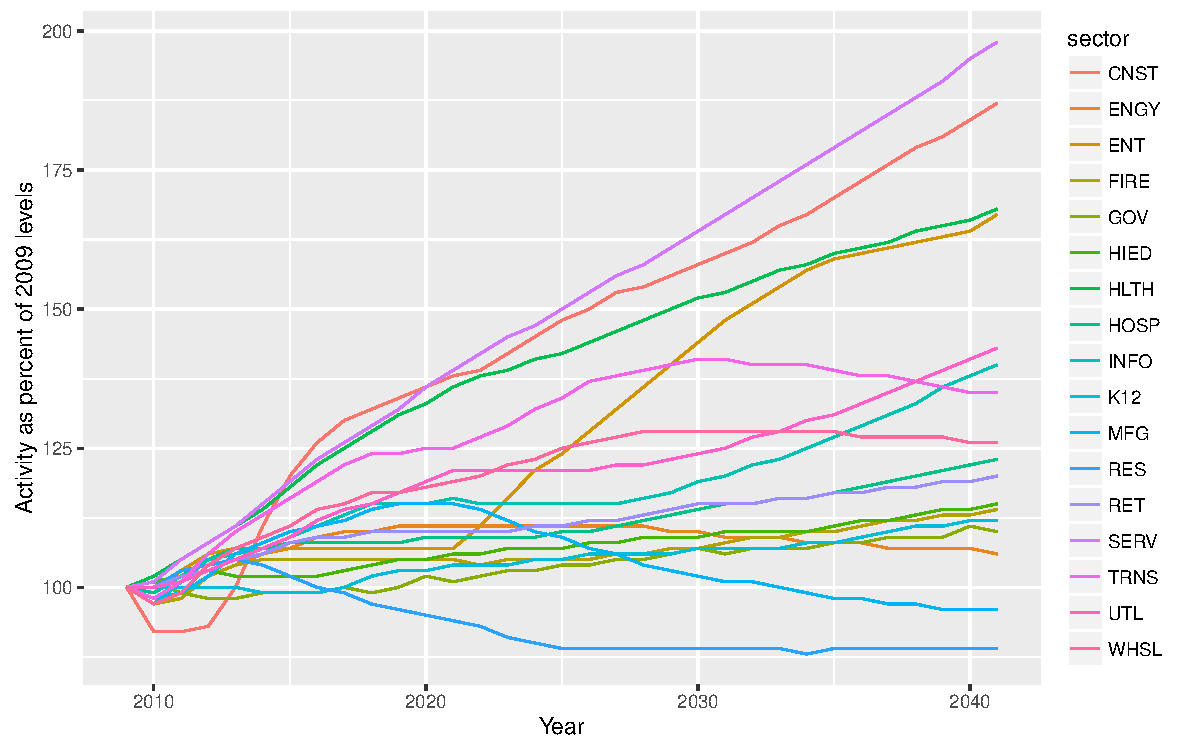
\includegraphics[width=6.5in]{ned/employment_forecast}
\caption{NED reference forecast employment, 2009-40}\label{fig:ned-employment-trends}
\end{figure}

\begin{figure}
\centering
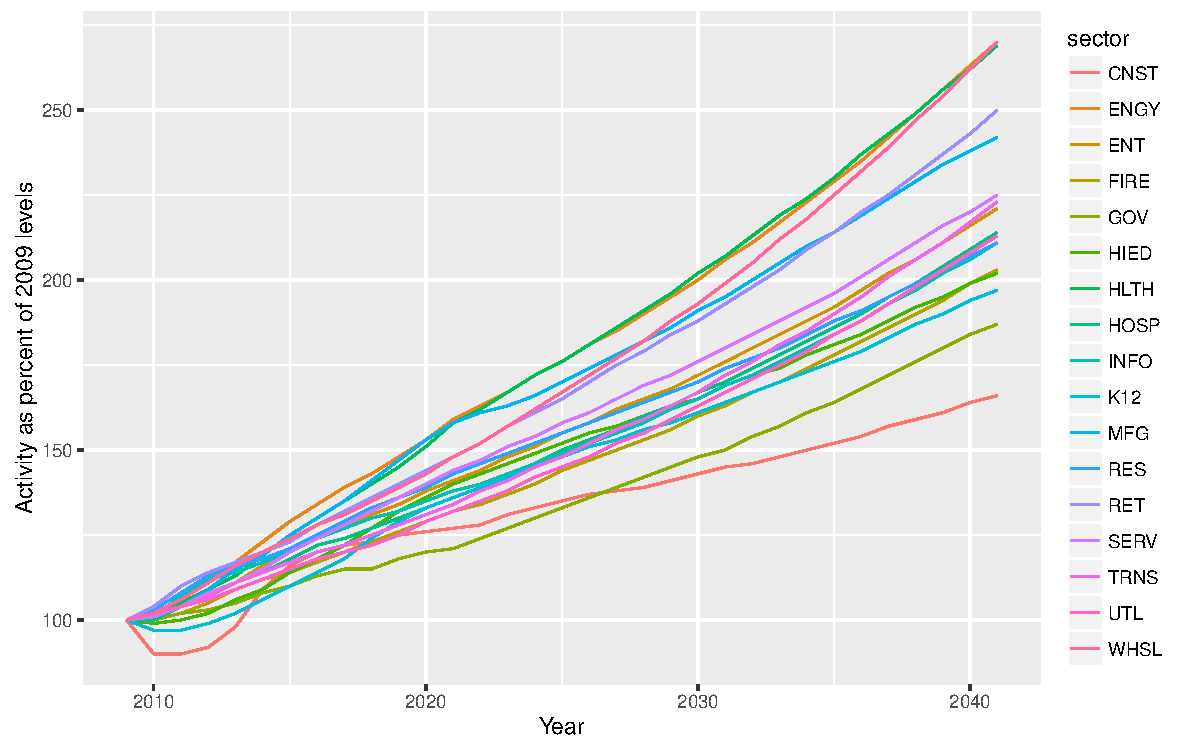
\includegraphics[width=6.5in]{ned/activity_forecast}
\caption{NED reference forecast industry activity, 2009-40}
\end{figure}

\begin{figure}
\centering
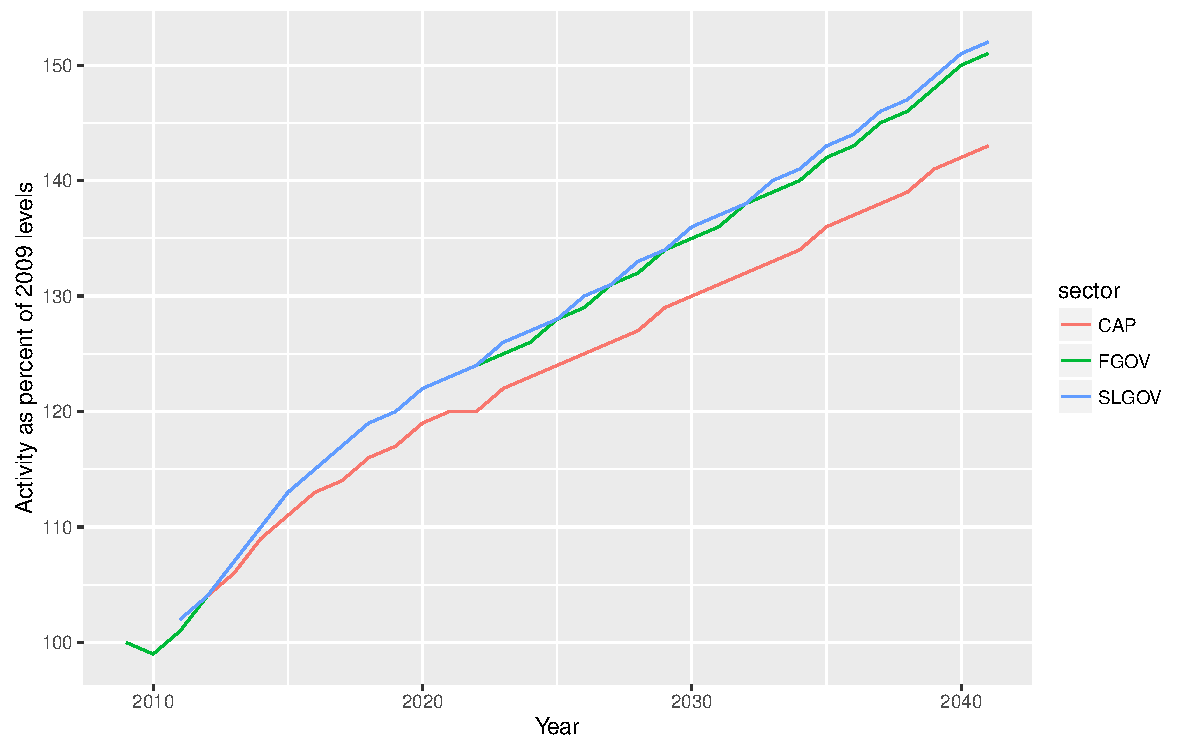
\includegraphics[width=6.5in]{ned/government_forecast.pdf}
\caption{NED reference forecast government activity, 2009-40}
\end{figure}

\begin{figure}
\centering
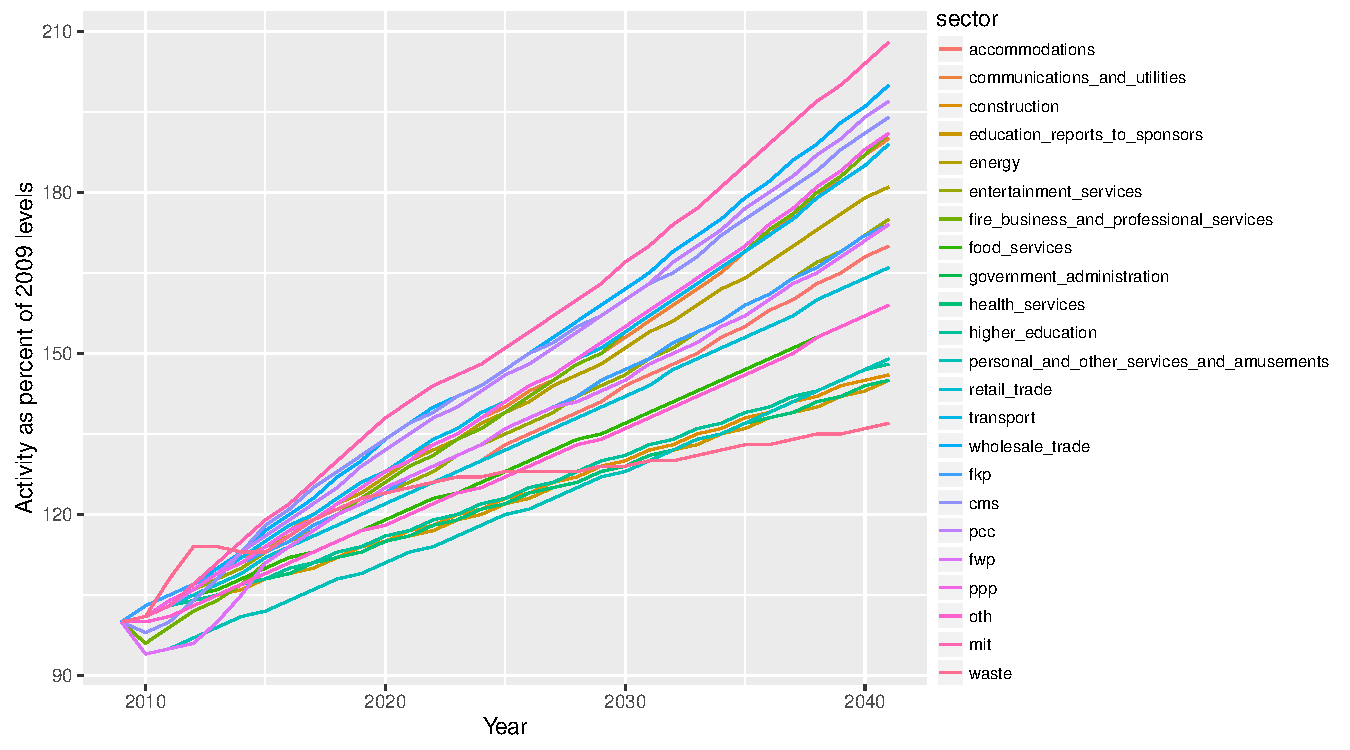
\includegraphics[width=7in]{ned/trade_forecast_imports.pdf}
\caption{NED reference forecast import activity, 2009-40}
\end{figure}

\begin{figure}
\centering
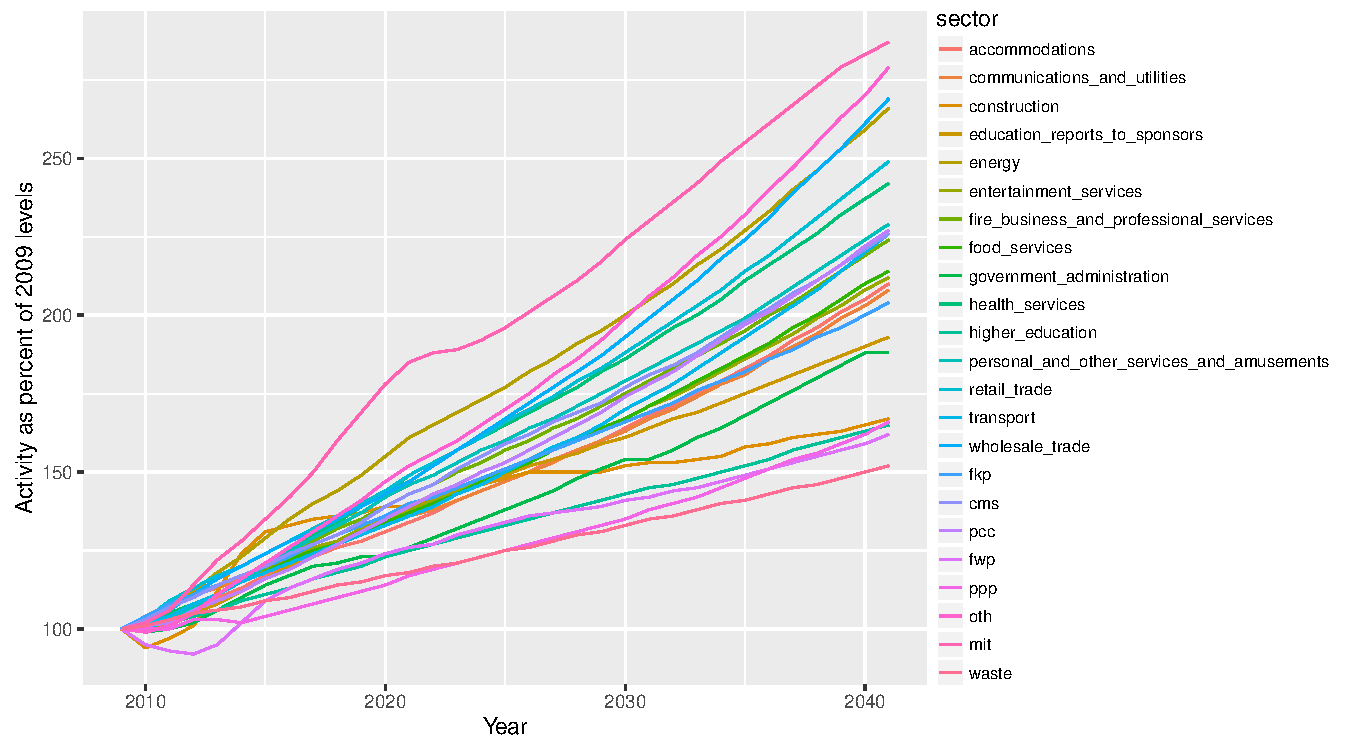
\includegraphics[width=7in]{ned/trade_forecast_exports}
\caption{NED reference forecast export activity, 2009-40}
\end{figure}

\begin{figure}
\centering
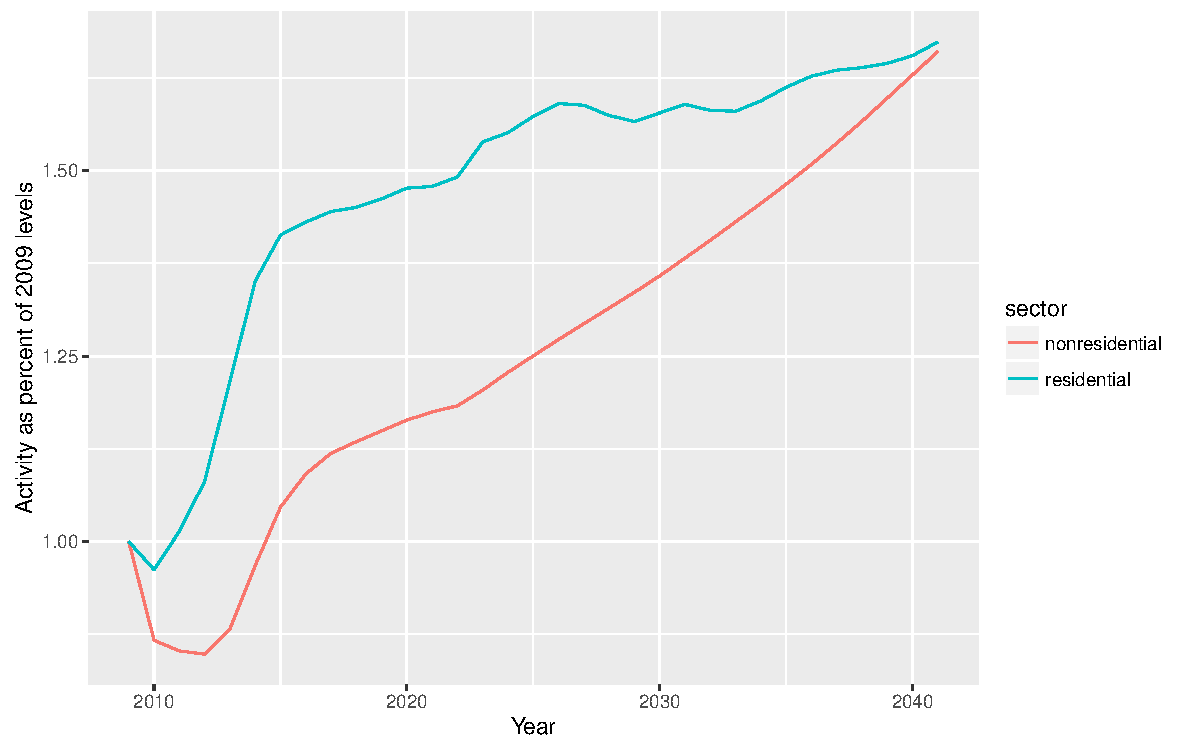
\includegraphics[width=6.5in]{ned/construction_forecast}
\caption{NED reference forecast annual construction dollars, 2009-40}
\label{fig:ned-construction-trends}
\end{figure}

\section{S3 Parameters}
The few estimated ED module coefficients, as well as the structure of the ED module (the number and composition of the equations) may be considered S3 parameters, subject to re-estimation and refinement as the full SWIM Model is tested and calibrated.

\section{Future Plans}
In the near future, the feedback features in NED will be made operational, parameterized, calibrated, and validated. A scenario generation tool also will be developed, allowing the model user to specify alternative scenarios. The scenario generation tool will produce files identical in format to those produced by the Baseline Scenario Generator, as well as files specifying alternative data for other modules. When an alternative scenario is run, those variables that differ from their counterparts in the baseline scenario will not be subject to change via feedback; the specification of the alternative scenario will be maintained. Other variables that are not a part of the specification may respond to feedback if feedback is enabled.


\chapter{Synthetic Population Generator (SPG) Module}\label{sec:spg-chapter}
In each year, the Synthetic Population Generator (SPG) Module generates a synthetic population consisting of a set of PUMS household records. In aggregate the resulting PUMS records conform to model-wide workers per household and age distributions and a set of model-wide employment by industry forecast determined by the NED module. Each household is assigned a home location consistent with alpha zone labor production (i.e., the home end of the labor flow in dollars) by occupation and household category (i.e., household income and size) determined by the AA module. The output produced by the SPG module is a synthetic population of persons and households with PUMS attributes and assigned a home alpha zone, in the PUMS file format. Later in the same model year, PT adjusts and adds to the Synthetic population attributes produced by SPG.

\section{Theoretical Basis}
The SPG Module uses a two-stage procedure, referred to as SPG1 and SPG2 to generate a synthetic population and to determine the alpha zone home locations for each household, respectively. The SPG1 procedure begins with the full set of PUMS records where the PUMS sample weights are adjusted using a table balancing methodology. The rows of the table consist of all the PUMS household records for the PUMAs covering the study area. The columns in the table correspond to the constraints to which the synthetic population is to conform; i.e. one column for each industry employment category (NED module constraint) and one column for each worker per household category and age group (exogenous constraint). The cell values in the table indicate the number of employed persons in each industry and age group for the household and which number of workers per household category the household record belongs. The table balancing procedure determines weights (i.e., expansion factors) for each PUMS household record so that when final weights have been determined, the weighted PUMS records conform to all the specified model-wide constraints, including NED regional employment totals by industry and model-wide households by workers per household and age categories. 

Once this weighted set of PUMS households is determined, SPG2 allocates each individual household to an alpha zone, respecting labor flow constraints from AA in the form of dollars of labor production by occupation and alpha zone and total households by household category by alpha zone.\footnote{AA operates at the beta zone level. A post-processing method disaggregates elements of the labor flows to alpha zones, based on endogenous land use inventory. This process is discussed in \S\ref{sec:aa-p-processor}.}

The two allocation procedures, generating the initial weight or count of each PUMS household record and allocating those households to alpha zones, are referred to as modules SPG1 and SPG2, respectively. SPG1 is a deterministic table balancing process, while SPG2 is a stochastic allocation of home location. The development of SPG draws from previous work by \citet{beckman96}, and code and notes shared by Mark Bradley from his work on a synthetic population generator for the Portland region.

\section{Quantity Definitions and Categories}
SPG1 operates at a model-wide level, while SPG2 operates at an alpha zone level. SPG1 takes a count of employees in aggregated industry sectors from the NED module to constrain the set of households generated. Since SPG uses US Census PUMS data, its sectors must be defined using Census categories. 

Two correspondence files (acs\_occupation\_2005\_2009.csv and pums\_to\_split\_industry.csv) map the PUMS industries and occupations to SWIM fully-split industries and occupations (previously noted in Tables \ref{tab:activity-industry} and \ref{tab:service-categories} on pages \pageref{tab:activity-industry} and \pageref{tab:service-categories}, respectively). Both fields are included in the resulting synthetic population files. This file also provides default values for industry and occupation based on most probable coding from the other PUMS fields, for records where PUMS had missing values.

The output of the SPG module is a synthetic population, written as a pair of files in PUMS file format:
\begin{itemize}
\item A SynPopH.csv file with household attributes
\item A corresponding SynPopP.csvfile with person attributes
\end{itemize}

\noindent The attributes of these files were shown previously in Figure \ref{fig:synthetic-attributes} (page \pageref{fig:synthetic-attributes}). Note that the original PUMS ID number (HH+Person), although not currently retained, could be added to allow linkage back to further household and person attributes if desired. 

\section{Component Models}

The SPG Module works in two stages, identified as SPG1 and SPG2. The SPG1 module determines a set of households in the model area consistent with the total employment by industry forecast by the NED module and the pre-specified distribution of households by number of workers per household. The number of total regional households by household size and household income categories, determined by the SPG1 module, is read as input by the AA module.

The SPG2 module reads labor dollars of production by alpha zone and number of households by (household size and household income) category by alpha zone information from the AA module as well as the set of PUMS household and person records as determined by SPG1. The zonal labor dollars of production are used to calculate probability distributions that determine the allocation of household records to home alpha zones. These components and their subtasks listed below are detailed in the remainder of this section:
\begin{itemize}
\item Population synthesis using a table balancing procedure (SPG1)
\item Household zone-level assignment (SPG2)
\end{itemize}

\noindent It should be noted that some information associated with the original PUMS record sample is updated by values calculated endogenously through the operation of the SWIM2module. SPG adds calculated fields to the SynPop files to match SWIM2 industry and occupation categories. Additionally, PT assigns a workplace location (based on the work end of the same AA labor flows) and updates the auto ownership information and adjusts other minor attributes. These updated values are retained in the personData.csv and householdData.csv files (see Figure \ref{fig:synthetic-attributes}) and the original SPG-generated synthetic population files are not updated. 

\subsection{Population Synthesis (SPG1)}
The NED module determines the total employment by industry for the entire model area.\footnote{The NED module produced population consistent with its employment estimates, but this is not used in subsequent SWIM2 modules. Future updates could constrain SPG to this population by matching absolute population by age, rather than age distributions.} The SPG1 module is intended to produce a set of households which are consistent with this forecasted employment. In other words, the SPG1 module determines a set of households with full attributes such that the number of employed persons by industry in those households matches the model-wide employment by industry forecast by the NED module. Unemployed households are also generated, consistent with the initial PUMS weights.

The NED model produces both jobs (employment) and workers (persons), reflecting the mismatch between US Bureau of Economic Analysis job data and Census worker data.NED forecasted jobs are adjusted by fixed factors into workers, accounting for mismatches between industry categories as well as workers working multiple jobs.

Besides total employment by industry category, two other important characteristic of the synthetic population are controlled for in SPG1. One is the distribution of employed persons in households. The distribution of households by number of workers per household is important for the PT module. For this reason, the SPG1 module is further constrained to match the model-wide distribution of workers per household, by year provided in an input file. A second controlled attribute in SPG1 is age distributions. This attribute is important to travel models, as the population ages and travel behavior changes.

At the close of the SPG1 table balancing procedure, the PUMS households have no spatial attributes. This model-wide count of households is input to AA to allocate household activity among zones. Thus, SPG1 operates after the NED module, but before the AA module.

\subsubsection{SPG1 Table balancing procedure: initial conditions}
The table balancing procedure used by the SPG1 module is described with reference to a simplified test case illustrated in Tables \ref{tab:spg1-balancing-initial} through \ref{tab:spg-after-iteration20}, which only covers one of the two controlled variables, worker per household but not person age. Adding age is equivalent to adding additional columns to the example. Table \ref{tab:spg1-balancing-initial} shows the test case data. The 25 rows in this table represent a sample of household records to be expanded. In the full model application, there are as many rows as there are PUMS records from all the PUMAs covering the model area. The columns in this table include an hh\_weight field, a set of industry fields and a set of household category fields, representing constraints defined for the procedure. The cell values in the hh\_weight field begin as the PUMS household weights and are changed systematically during the balancing procedure. For simplicity, the test case assumes all PUMS household weights have a value of 1.0. In the full model application, each cell value would be multiplied by the PUMS household record weight (i.e., PUMS HOUSWGT field value). The cell value in the constraint fields are dependent on the hh\_weight cell value and thus are also modified by the table balancing procedure. At the end of the procedure, the final values in the hh\_weight field indicate the number of times each sample household record should be replicated in the TM synthetic population. The table balancing procedure is run iteratively, with constraint cell values changing as a result of changes to the hh\_weight values until all constraint field totals match the specified constraints.

\begin{sidewaystable}  % Table 4 1
\centering
\caption{Initial household records and constraints for SPG1 matrix balancing procedure}
\label{tab:spg1-balancing-initial}
\small
\begin{tabular}{c*{12}r}
\hline
Household & hh weight & Retail & Educ & Service & Govt & Mfr & Other & 0 worker & 1 worker & 2 workers & 3 workers & 4 workers \\
\hline
1 & & 1 & 1 & & & & & 0 & 0 & 1 & 0 & 0 \\
\gray 2 & & & & & & & 1 & 0 & 1 & 0 & 0 & 0 \\
3 & & 2 & & 1 & & & & 0 & 0 & 0 & 1 & 0 \\
\gray 4 & & & & 1 & & 1 & & 0 & 0 & 1 & 0 & 0 \\
5 & & & 2 & & & & 1 & 0 & 0 & 0 & 1 & 0 \\
\gray 6 & & & & & 2 & & 2 & 0 & 0 & 0 & 0 & 1 \\
7 & & & & & & & & 1 & 0 & 0 & 0 & 0 \\
\gray 8 & & 1 & & & & & & 0 & 1 & 0 & 0 & 0 \\
9 & & 1 & & & 1 & 1 & 1 & 0 & 0 & 0 & 0 & 1 \\
\gray 10 & & & & 1 & & & & 0 & 1 & 0 & 0 & 0 \\
11 & & & 1 & & 2 & & & 0 & 0 & 0 & 1 & 0 \\
\gray 12 & & & & & 1 & & 1 & 0 & 0 & 1 & 0 & 0 \\
13 & & & 1 & 1 & 1 & & 1 & 0 & 0 & 0 & 0 & 1 \\
\gray 14 & & 1 & 2 & & & & & 0 & 0 & 0 & 1 & 0 \\
15 & & 1 & & 1 & 1 & & & 0 & 0 & 0 & 1 & 0 \\
\gray 16 & & & & & & & & 1 & 0 & 0 & 0 & 0 \\
17 & & & 1 & 1 & & & & 0 & 0 & 1 & 0 & 0 \\
\gray 18 & & & & & 2 & & & 0 & 0 & 1 & 0 & 0 \\
19 & & & & & & & 1 & 0 & 1 & 0 & 0 & 0 \\
\gray 20 & & & & & & & 1 & 0 & 1 & 0 & 0 & 0 \\
21 & & & & & 1 & & 1 & 0 & 0 & 1 & 0 & 0 \\
\gray 22 & & 1 & & & & & & 0 & 1 & 0 & 0 & 0 \\
23 & & & & & & & 1 & 0 & 1 & 0 & 0 & 0 \\
\gray 24 & & 1 & & & & 1 & & 0 & 0 & 1 & 0 & 0 \\
25 & & 1 & & 1 & & & & 0 & 0 & 1 & 0 & 0 \\
\gray  & & 10 & 8 & 7 & 11 & 3 & 11 & 2 & 7 & 8 & 5 & 3 \\
 & & 0.2 & 0.16 & 0.14 & 0.22 & 0.06 & 0.22 & 0.08 & 0.28 & 0.32 & 0.2 & 0.12 \\
\hline
\rowcolor{yellow!10}\multicolumn{8}{l}{Regional total workers by employment category -- employment targets} & \multicolumn{5}{l}{Households by workers per households -- household targets} \\
\rowcolor{yellow!10} & & 2,150 & 1,800 & 2,800 & 2,200 & 1,950 & 3,000 & 556 & 1,946 & 2,224 & 1,390 & 834 \\
\rowcolor{yellow!10} & & 15.47\% & 12.95\% & 20.14\% & 15.83\% & 14.03\% & 21.58\% & 8.0\% & 28.0\% & 32.0\% & 20.0\% & 12.0\% \\
\rowcolor{yellow!10} & & & & & & & & & & & &  \\
\rowcolor{yellow!10} \multicolumn{7}{r}{Total workers =} & 13,900 & \multicolumn{4}{r}{Total households =} & 6,950 \\
\hline
\multicolumn{13}{l}{\footnotesize Note: For simplicity, this test case assumes an initial hh\_weight of 1.0 for all households, rather than household-specific PUMS weight.} \\
\end{tabular}
\end{sidewaystable}

In Table \ref{tab:spg1-balancing-initial}, the constraints specified for the test case are shown highlighted in yellow. The numbers shown in bold italics font in the lower highlighted area indicate constraints for the SPG1 procedure. The model-wide employment by industry category from the NED module adjusted using jobs-to-worker factors and relative frequencies of the number of workers per household by household category are read as exogenous inputs. Jobs-to-worker factors were required to adjust for multiple jobs per person, absentees and other unspecified differences between NED and SPG data sources. From these absolute worker totals, the relative frequency by industry category is determined. Likewise, from the relative frequencies of households by household category and NED-based workers over all industries, absolute number of model-wide households in each household category can be determined. The equation to calculate total households follows. For the Table \ref{tab:spg1-balancing-initial} test case, the model-wide workers ($\sum W_i$) are constrained to 13,900 workers, leading to a value of 6,950 households (H).

\begin{equation}
H = \sum_n n \times Share_n / \sum_i W_i
\end{equation}
\noindent where:
\begin{align*}
n &= \text{number of workers per household (0, 1, 2, 3 or 4)} \\
i &= \text{index of aggregated industry sector categories} \\
H &= \text{SPG target for number of model-wide households} \\
Share_n &= \text{Target share of $n$ worker households of all households (exogenous)} \\
W_i &= \text{SPG target for number of model-wide workers in industry sector $i$}
\end{align*}

The starting conditions for the table balancing procedure are illustrated in Table \ref{tab:spg1-balancing-initial}. The household records and their initial constraint field values are determined from the Census PUMS dataset. The starting values of the hh\_weight field would be the PUMS household weights (assumed to be 1 for all households in the test case of Table \ref{tab:spg1-balancing-initial} or could be adjusted by the user). The constraint values come from forecasts of regional employment by category (NED module) and a specified distribution of household attribute values (weighted Census PUMS or STF dataset).

\subsubsection{SPG1 table balancing procedure: first iteration}

An expanded version of the process is shown in Table \ref{tab:spg-after-initial-expansion}, after the hh\_weight cell values are initialized. To do so, an initial hh\_weight expansion factor is calculated as a ratio of the target and sample count of workers by industry, as follows:
\begin{equation}
InitFactor = \sum_i W_i / \sum_i SampleW_i
\end{equation}
\noindent where:
\begin{align*}
i &= \text{index of industry sector categories} \\
InitFactor &= \text{initial household expansion factor (initial hh\_weight)} \\
W_i &= \text{target workers by industry $i$} \\
SampleW_i &= \text{household weight for each PUMS sample worker in industry $i$}
\end{align*}

\begin{sidewaystable}  % Table 4 2
\centering
\caption{SPG table balancing procedure example: after initial hh\_weight expansion factor}
\label{tab:spg-after-initial-expansion}
\small
\begin{tabular}{c*{12}{r}}
\vspace{-8pt} \\
\multicolumn{8}{l}{Initial expansion factor = 278} \\
\hline
Household & hh weight & Retail & Educ & Service & Govt & Mfr & Other & 0 worker & 1 worker & 2 workers & 3 workers & 4 workers \\
\hline
1 & 278 & 278 & 278 & 0 & 0 & 0 & 0 & 0 & 0 & 278 & 0 & 0 \\
\gray 2 & 278 & 0 & 0 & 0 & 0 & 0 & 278 & 0 & 278 & 0 & 0 & 0 \\
3 & 278 & 556 & 0 & 278 & 0 & 0 & 0 & 0 & 0 & 0 & 278 & 0 \\
\gray 4 & 278 & 0 & 0 & 278 & 0 & 278 & 0 & 0 & 0 & 278 & 0 & 0 \\
5 & 278 & 0 & 556 & 0 & 0 & 0 & 278 & 0 & 0 & 0 & 278 & 0 \\
\gray 6 & 278 & 0 & 0 & 0 & 556 & 0 & 556 & 0 & 0 & 0 & 0 & 278 \\
7 & 278 & 0 & 0 & 0 & 0 & 0 & 0 & 278 & 0 & 0 & 0 & 0 \\
\gray 8 & 278 & 278 & 0 & 0 & 0 & 0 & 0 & 0 & 278 & 0 & 0 & 0 \\
9 & 278 & 278 & 0 & 0 & 278 & 278 & 278 & 0 & 0 & 0 & 0 & 278 \\
\gray 10 & 278 & 0 & 0 & 278 & 0 & 0 & 0 & 0 & 278 & 0 & 0 & 0 \\
11 & 278 & 0 & 278 & 0 & 556 & 0 & 0 & 0 & 0 & 0 & 278 & 0 \\
\gray 12 & 278 & 0 & 0 & 0 & 278 & 0 & 278 & 0 & 0 & 278 & 0 & 0 \\
13 & 278 & 0 & 278 & 278 & 278 & 0 & 278 & 0 & 0 & 0 & 0 & 278 \\
\gray 14 & 278 & 278 & 556 & 0 & 0 & 0 & 0 & 0 & 0 & 0 & 278 & 0 \\
15 & 278 & 278 & 0 & 278 & 278 & 0 & 0 & 0 & 0 & 0 & 278 & 0 \\
\gray 16 & 278 & 0 & 0 & 0 & 0 & 0 & 0 & 278 & 0 & 0 & 0 & 0 \\
17 & 278 & 0 & 278 & 278 & 0 & 0 & 0 & 0 & 0 & 278 & 0 & 0 \\
\gray 18 & 278 & 0 & 0 & 0 & 556 & 0 & 0 & 0 & 0 & 278 & 0 & 0 \\
19 & 278 & 0 & 0 & 0 & 0 & 0 & 278 & 0 & 278 & 0 & 0 & 0 \\
\gray 20 & 278 & 0 & 0 & 0 & 0 & 0 & 278 & 0 & 278 & 0 & 0 & 0 \\
21 & 278 & 0 & 0 & 0 & 278 & 0 & 278 & 0 & 0 & 278 & 0 & 0 \\
\gray 22 & 278 & 278 & 0 & 0 & 0 & 0 & 0 & 0 & 278 & 0 & 0 & 0 \\
23 & 278 & 0 & 0 & 0 & 0 & 0 & 278 & 0 & 278 & 0 & 0 & 0 \\
\gray 24 & 278 & 278 & 0 & 0 & 0 & 278 & 0 & 0 & 0 & 278 & 0 & 0 \\
25 & 278 & 278 & 0 & 278 & 0 & 0 & 0 & 0 & 0 & 278 & 0 & 0 \\
\hline
 &  & 2,780 & 2,224 & 1,946 & 3,058 & 834 & 3,058 & 556 & 1,946 & 2,224 & 1,390 & 834 \\
 &  & 20.00\% & 16.00\% & 14.00\% & 22.00\% & 6.00\% & 22.00\% & 8.00\% & 28.00\% & 32.00\% & 20.00\% & 12.00\% \\
\rowcolor{yellow!10} \cellcolor{white}& \cellcolor{white} & 15.47\% & 12.95\% & 20.14\% & 15.83\% & 14.03\% & 21.58\% & 8.00\% & 28.00\% & 32.00\% & 20.00\% & 12.00\% \\
 &  &  &  &  &  &  & 13,900 &  &  &  &  & 6,950 \\
\hline
\end{tabular}
\end{sidewaystable}

Applying the expanded initial hh\_weight values to all cells, results in an initial worker and household count estimate in each field cell, as shown in Table \ref{tab:spg-after-initial-expansion} (in the example, InitFactor = 13900/50 = 278). The column sums provide the total workers and total households estimated by category after this initial balancing step. Below the column sums in Table \ref{tab:spg-after-initial-expansion}, the resulting relative distribution of workers and households by category are shown. This can be compared with the highlighted targeted distributions (consistent with those estimated in Table \ref{tab:spg1-balancing-initial}). The difference between the calculated field frequencies and their corresponding target frequencies indicates the amount of adjustment needed by category in order to satisfy all constraints. When this difference is minimal (meets a user-defined target threshold) for all constraints, the table is considered balanced.

In order to attain a balanced table, a series of systematic adjustments must be applied through the course of multiple iterations. In each iteration adjustment factors are calculated for each field constraint in turn. An adjustment factor is calculated as the ratio of the targeted count and most recent sample count for that field, as follows:
\begin{equation}   % 4.04
AdjFactor_k = TargetCount_k / \sum_r SampleCount_{k,r}
\end{equation}
\noindent where:
\begin{align*}
k &= \text{index for constraint field category (industry or household category)} \\
r &= \text{index for sample household record} \\
AdjFactor_k &= \text{sample adjustment factor for field $k$} \\
TargetCount_k &= \text{targeted count for field category $k$} \\
SampleCount_{k,r} &= \text{sample count in field category $k$ from household record $r$}
\end{align*} 

The process begins by calculating the adjustment factor for the first field category. This adjustment factor updates the initial hh\_weight values if and only if those households (rows) have non-zero entries in the field being adjusted. Subsequent updates to all field cell values are made and columns summed. After the adjustment factor is calculated and applied, the column sum in that field will match the targeted value (in absolute terms, not relative frequency). 

Continuing our example, an adjustment factor of 0.77 (2150/2780) was calculated for the retail field. The results of applying this adjustment factor are shown in Table \ref{tab:spg-after-retail-iteration1}. All households (rows) in the sample with non-zero retail workers were assigned a hh\_weight of 215 (278*0.77). For example, household 1 has non-zero employed persons in constraint field 1, so its hh\_weight is adjusted, while Household 2 has zero employed persons in constraint field 1, so its hh\_weight is not. These new hh\_weights are then applied to the other fields, leading to modified column sums for each field. Note also that the column sum of constraint field 1 matches the target exactly. The relative frequency and target relative frequency do not match at this point because the total workers estimated by the current set of hh\_weights are too low (12,577 in sample versus 13,900 target).

\begin{sidewaystable}  % Table 4 3
\centering
\caption{SPG table balancing procedure example: after iteration 1 adjustment to retail field}
\label{tab:spg-after-retail-iteration1}
\small
\begin{tabular}{c*{12}{r}}
\vspace{-8pt} \\
\multicolumn{8}{l}{Balancing factor = 0.773381295} \\
\hline
Household & hh weight & Retail & Educ & Service & Govt & Mfr & Other & 0 worker & 1 worker & 2 workers & 3 workers & 4 workers \\
\hline
1 & 215 & 215 & 215 & 0 & 0 & 0 & 0 & 0 & 0 & 215 & 0 & 0 \\
\gray 2 & 278 & 0 & 0 & 0 & 0 & 0 & 278 & 0 & 278 & 0 & 0 & 0 \\
3 & 215 & 430 & 0 & 215 & 0 & 0 & 0 & 0 & 0 & 0 & 215 & 0 \\
\gray 4 & 278 & 0 & 0 & 278 & 0 & 278 & 0 & 0 & 0 & 278 & 0 & 0 \\
5 & 278 & 0 & 556 & 0 & 0 & 0 & 278 & 0 & 0 & 0 & 278 & 0 \\
\gray 6 & 278 & 0 & 0 & 0 & 556 & 0 & 556 & 0 & 0 & 0 & 0 & 278 \\
7 & 278 & 0 & 0 & 0 & 0 & 0 & 0 & 278 & 0 & 0 & 0 & 0 \\
\gray 8 & 215 & 215 & 0 & 0 & 0 & 0 & 0 & 0 & 215 & 0 & 0 & 0 \\
9 & 215 & 215 & 0 & 0 & 215 & 215 & 215 & 0 & 0 & 0 & 0 & 215 \\
\gray 10 & 278 & 0 & 0 & 278 & 0 & 0 & 0 & 0 & 278 & 0 & 0 & 0 \\
11 & 278 & 0 & 278 & 0 & 556 & 0 & 0 & 0 & 0 & 0 & 278 & 0 \\
\gray 12 & 278 & 0 & 0 & 0 & 278 & 0 & 278 & 0 & 0 & 278 & 0 & 0 \\
13 & 278 & 0 & 278 & 278 & 278 & 0 & 278 & 0 & 0 & 0 & 0 & 278 \\
\gray 14 & 215 & 215 & 430 & 0 & 0 & 0 & 0 & 0 & 0 & 0 & 215 & 0 \\
15 & 215 & 215 & 0 & 215 & 215 & 0 & 0 & 0 & 0 & 0 & 215 & 0 \\
\gray 16 & 278 & 0 & 0 & 0 & 0 & 0 & 0 & 278 & 0 & 0 & 0 & 0 \\
17 & 278 & 0 & 278 & 278 & 0 & 0 & 0 & 0 & 0 & 278 & 0 & 0 \\
\gray 18 & 278 & 0 & 0 & 0 & 556 & 0 & 0 & 0 & 0 & 278 & 0 & 0 \\
19 & 278 & 0 & 0 & 0 & 0 & 0 & 278 & 0 & 278 & 0 & 0 & 0 \\
\gray 20 & 278 & 0 & 0 & 0 & 0 & 0 & 278 & 0 & 278 & 0 & 0 & 0 \\
21 & 278 & 0 & 0 & 0 & 278 & 0 & 278 & 0 & 0 & 278 & 0 & 0 \\
\gray 22 & 215 & 215 & 0 & 0 & 0 & 0 & 0 & 0 & 215 & 0 & 0 & 0 \\
23 & 278 & 0 & 0 & 0 & 0 & 0 & 278 & 0 & 278 & 0 & 0 & 0 \\
\gray 24 & 215 & 215 & 0 & 0 & 0 & 215 & 0 & 0 & 0 & 215 & 0 & 0 \\
25 & 215 & 215 & 0 & 215 & 0 & 0 & 0 & 0 & 0 & 215 & 0 & 0 \\
\hline
 &  & 2,150 & 2,035 & 1,757 & 2,932 & 708 & 2,995 & 556 & 1,820 & 2,035 & 1,201 & 771 \\
 &  & 17.09\% & 16.18\% & 13.97\% & 23.31\% & 5.63\% & 23.81\% & 8.71\% & 28.51\% & 31.88\% & 18.82\% & 12.08\% \\
\rowcolor{yellow!10} \cellcolor{white} & \cellcolor{white} & 15.47\% & 12.95\% & 20.14\% & 15.83\% & 14.03\% & 21.58\% & 8.00\% & 28.00\% & 32.00\% & 20.00\% & 12.00\% \\
 &  &  &  &  &  &  & 12,577 &  &  &  &  & 6,383 \\
\hline
\end{tabular}
\end{sidewaystable}

At this point, the process is repeated in the same manner for the each field in turn; calculating an adjustment factor, updating the hh\_weight for those household with non-zero cell values in that field, updating the remaining field cells and the associated column sums. The results of making these adjustments to field 2 are shown in Table \ref{tab:spg-after-education-iteration1}. Note that although the column sum for field 2 now matches the target exactly, the column sum of field 1 no longer matches its target, but is still somewhat close.

\begin{sidewaystable}  % Table 4 4
\centering
\caption{SPG table balancing procedure example: after iteration 1 adjustment to education field}
\label{tab:spg-after-education-iteration1}
\small
\begin{tabular}{c*{12}{r}}
\vspace{-8pt} \\
\multicolumn{8}{l}{Balancing factor = 0.884520885} \\
\hline
Household & hh weight & Retail & Educ & Service & Govt & Mfr & Other & 0 worker & 1 worker & 2 workers & 3 workers & 4 workers \\
\hline
1 & 190.17 & 190.17 & 190.17 & 0 & 0 & 0 & 0 & 0 & 0 & 190.17 & 0 & 0 \\
\gray 2 & 278 & 0 & 0 & 0 & 0 & 0 & 278 & 0 & 278 & 0 & 0 & 0 \\
3 & 215 & 430 & 0 & 215 & 0 & 0 & 0 & 0 & 0 & 0 & 215 & 0 \\
\gray 4 & 278 & 0 & 0 & 278 & 0 & 278 & 0 & 0 & 0 & 278 & 0 & 0 \\
5 & 245.90 & 0 & 491.79 & 0 & 0 & 0 & 245.90 & 0 & 0 & 0 & 245.90 & 0 \\
\gray 6 & 278 & 0 & 0 & 0 & 556 & 0 & 556 & 0 & 0 & 0 & 0 & 278 \\
7 & 278 & 0 & 0 & 0 & 0 & 0 & 0 & 278 & 0 & 0 & 0 & 0 \\
\gray 8 & 215 & 215 & 0 & 0 & 0 & 0 & 0 & 0 & 215 & 0 & 0 & 0 \\
9 & 215 & 215 & 0 & 0 & 215 & 215 & 215 & 0 & 0 & 0 & 0 & 215 \\
\gray 10 & 278 & 0 & 0 & 278 & 0 & 0 & 0 & 0 & 278 & 0 & 0 & 0 \\
11 & 245.90 & 0 & 245.90 & 0 & 491.79 & 0 & 0 & 0 & 0 & 0 & 245.90 & 0 \\
\gray 12 & 278 & 0 & 0 & 0 & 278 & 0 & 278 & 0 & 0 & 278 & 0 & 0 \\
13 & 245.90 & 0 & 245.90 & 245.90 & 245.90 & 0 & 245.90 & 0 & 0 & 0 & 0 & 245.90 \\
\gray 14 & 190.17 & 190.17 & 380.34 & 0 & 0 & 0 & 0 & 0 & 0 & 0 & 190.17 & 0 \\
15 & 215 & 215 & 0 & 215 & 215 & 0 & 0 & 0 & 0 & 0 & 215 & 0 \\
\gray 16 & 278 & 0 & 0 & 0 & 0 & 0 & 0 & 278 & 0 & 0 & 0 & 0 \\
17 & 245.90 & 0 & 245.90 & 245.90 & 0 & 0 & 0 & 0 & 0 & 245.90 & 0 & 0 \\
\gray 18 & 278 & 0 & 0 & 0 & 556 & 0 & 0 & 0 & 0 & 278 & 0 & 0 \\
19 & 278 & 0 & 0 & 0 & 0 & 0 & 278 & 0 & 278 & 0 & 0 & 0 \\
\gray 20 & 278 & 0 & 0 & 0 & 0 & 0 & 278 & 0 & 278 & 0 & 0 & 0 \\
21 & 278 & 0 & 0 & 0 & 278 & 0 & 278 & 0 & 0 & 278 & 0 & 0 \\
\gray 22 & 215 & 215 & 0 & 0 & 0 & 0 & 0 & 0 & 215 & 0 & 0 & 0 \\
23 & 278 & 0 & 0 & 0 & 0 & 0 & 278 & 0 & 278 & 0 & 0 & 0 \\
\gray 24 & 215 & 215 & 0 & 0 & 0 & 215 & 0 & 0 & 0 & 215 & 0 & 0 \\
25 & 215 & 215 & 0 & 215 & 0 & 0 & 0 & 0 & 0 & 215 & 0 & 0 \\
\hline
 &  & 2100.34 & 1800 & 1692.79 & 2835.69 & 708 & 2930.79 & 556 & 1820 & 1978.07 & 1111.97 & 738.90 \\
 &  & 17.40\% & 14.92\% & 14.03\% & 23.50\% & 5.87\% & 24.29\% & 8.96\% & 29.33\% & 31.88\% & 17.92\% & 11.91\% \\
\rowcolor{yellow!10} \cellcolor{white} & \cellcolor{white} & 15.47\% & 12.95\% & 20.14\% & 15.83\% & 14.03\% & 21.58\% & 8.00\% & 28.00\% & 32.00\% & 20.00\% & 12.00\% \\
 &  &  &  &  &  &  & 12067.622 &  &  &  &  & 6204.931 \\
\hline
\end{tabular}
\end{sidewaystable}

Subsequent adjustments are made for each of the industry fields and then each household category field until all fields have been updated. Note that after the last household field, only that field will be guaranteed to match its target, although the other fields should be closer in general than before the adjustments were made and the table will have the correct total expanded workers and total expanded households compared to targets. The adjustment of the last household constraint field signals the end of the first table balancing procedure iteration. The household sample resulting from the first table balancing iteration is shown in Table \ref{tab:spg-after-iteration1}.

\begin{sidewaystable}  % Table 4 5
\centering
\caption{SPG table balancing procedure example: after iteration 1}
\label{tab:spg-after-iteration1}
\small
\begin{tabular}{c*{12}{r}}
\vspace{-8pt} \\
\multicolumn{8}{l}{Balancing factor = 0.9238079} \\
\hline
Household & hh weight & Retail & Educ & Service & Govt & Mfr & Other & 0 worker & 1 worker & 2 workers & 3 workers & 4 workers \\
\hline
1 & 133.75 & 133.75 & 133.75 & 0 & 0 & 0 & 0 & 0 & 0 & 133.75 & 0 & 0 \\
\gray 2 & 279.39 & 0 & 0 & 0 & 0 & 0 & 279.39 & 0 & 279.39 & 0 & 0 & 0 \\
3 & 400.88 & 801.77 & 0 & 400.88 & 0 & 0 & 0 & 0 & 0 & 0 & 400.88 & 0 \\
\gray 4 & 763.83 & 0 & 0 & 763.83 & 0 & 763.83 & 0 & 0 & 0 & 763.83 & 0 & 0 \\
5 & 299.23 & 0 & 598.46 & 0 & 0 & 0 & 299.23 & 0 & 0 & 0 & 299.23 & 0 \\
\gray 6 & 194.42 & 0 & 0 & 0 & 388.84 & 0 & 388.84 & 0 & 0 & 0 & 0 & 194.42 \\
7 & 278.00 & 0 & 0 & 0 & 0 & 0 & 0 & 278 & 0 & 0 & 0 & 0 \\
\gray 8 & 200.16 & 200.16 & 0 & 0 & 0 & 0 & 0 & 0 & 200.16 & 0 & 0 & 0 \\
9 & 355.14 & 355.14 & 0 & 0 & 355.14 & 355.14 & 355.14 & 0 & 0 & 0 & 0 & 355.14 \\
\gray 10 & 428.10 & 0 & 0 & 428.10 & 0 & 0 & 0 & 0 & 428.10 & 0 & 0 & 0 \\
11 & 194.39 & 0 & 194.39 & 0 & 388.77 & 0 & 0 & 0 & 0 & 0 & 194.39 & 0 \\
\gray 12 & 148.01 & 0 & 0 & 0 & 148.01 & 0 & 148.01 & 0 & 0 & 148.01 & 0 & 0 \\
13 & 284.45 & 0 & 284.45 & 284.45 & 284.45 & 0 & 284.45 & 0 & 0 & 0 & 0 & 284.45 \\
\gray 14 & 214.37 & 214.37 & 428.75 & 0 & 0 & 0 & 0 & 0 & 0 & 0 & 214.37 & 0 \\
15 & 281.13 & 281.13 & 0 & 281.13 & 281.13 & 0 & 0 & 0 & 0 & 0 & 281.13 & 0 \\
\gray 16 & 278.00 & 0 & 0 & 0 & 0 & 0 & 0 & 278 & 0 & 0 & 0 & 0 \\
17 & 286.05 & 0 & 286.05 & 286.05 & 0 & 0 & 0 & 0 & 0 & 286.05 & 0 & 0 \\
\gray 18 & 137.11 & 0 & 0 & 0 & 274.22 & 0 & 0 & 0 & 0 & 137.11 & 0 & 0 \\
19 & 279.39 & 0 & 0 & 0 & 0 & 0 & 279.39 & 0 & 279.39 & 0 & 0 & 0 \\
\gray 20 & 279.39 & 0 & 0 & 0 & 0 & 0 & 279.39 & 0 & 279.39 & 0 & 0 & 0 \\
21 & 148.01 & 0 & 0 & 0 & 148.01 & 0 & 148.01 & 0 & 0 & 148.01 & 0 & 0 \\
\gray 22 & 200.16 & 200.16 & 0 & 0 & 0 & 0 & 0 & 0 & 200.16 & 0 & 0 & 0 \\
23 & 279.39 & 0 & 0 & 0 & 0 & 0 & 279.39 & 0 & 279.39 & 0 & 0 & 0 \\
\gray 24 & 357.14 & 357.14 & 0 & 0 & 0 & 357.14 & 0 & 0 & 0 & 357.14 & 0 & 0 \\
25 & 250.11 & 250.11 & 0 & 250.11 & 0 & 0 & 0 & 0 & 0 & 250.11 & 0 & 0 \\
\hline
 & & 2793.72 & 1925.83 & 2694.54 & 2268.56 & 1476.10 & 2741.24 & 556 & 1946 & 2224 & 1390 & 834 \\
 & & 20.10\% & 13.85\% & 19.39\% & 16.32\% & 10.62\% & 19.72\% & 8.00\% & 28.00\% & 32.00\% & 20.00\% & 12.00\% \\
\rowcolor{yellow!10} \cellcolor{white} & \cellcolor{white} & 15.47\% & 12.95\% & 20.14\% & 15.83\% & 14.03\% & 21.58\% & 8.00\% & 28.00\% & 32.00\% & 20.00\% & 12.00\% \\
 &  &  &  &  &  &  & 13900 &  &  &  &  & 6950 \\
\hline
\end{tabular}
\end{sidewaystable}

\subsubsection{SPG1 table balancing procedure: subsequent iterations}
After the end of the first table balancing iteration, a check is performed to determine if any constraint fields differ from their targets. If any differ by more than a user-specified acceptable error, then another iteration of table balancing is performed. The hh\_weights from the previous iteration are adjusted at the beginning of the new iteration, as the new iteration again calculates and applies adjustment factors for each constraint field, as described above. The resulting table after two full table balancing iterations is shown in Table \ref{tab:spg-after-iteration2}, while the results at the end of 20 table balancing iterations are shown in Table \ref{tab:spg-after-iteration20}. 

\begin{sidewaystable}  % Table 4 6
\centering
\caption{SPG table balancing procedure example: after iteration 2}
\label{tab:spg-after-iteration2}
\small
\begin{tabular}{c*{12}{r}}
\vspace{-8pt} \\
\multicolumn{8}{l}{Balancing factor = 0.869082045} \\
\hline
Household & hh weight & Retail & Educ & Service & Govt & Mfr & Other & 0 worker & 1 worker & 2 workers & 3 workers & 4 workers \\
\hline
1 & 85.91 & 85.91 & 85.91 & 0 & 0 & 0 & 0 & 0 & 0 & 85.91 & 0 & 0 \\
\gray 2 & 292.55 & 0 & 0 & 0 & 0 & 0 & 292.55 & 0 & 292.55 & 0 & 0 & 0 \\
3 & 379.55 & 759.10 & 0 & 379.55 & 0 & 0 & 0 & 0 & 0 & 0 & 379.55 & 0 \\
\gray 4 & 991.83 & 0 & 0 & 991.83 & 0 & 991.83 & 0 & 0 & 0 & 991.83 & 0 & 0 \\
5 & 349.07 & 0 & 698.14 & 0 & 0 & 0 & 349.07 & 0 & 0 & 0 & 349.07 & 0 \\
\gray 6 & 181.45 & 0 & 0 & 0 & 362.89 & 0 & 362.89 & 0 & 0 & 0 & 0 & 181.45 \\
7 & 278.00 & 0 & 0 & 0 & 0 & 0 & 0 & 278.00 & 0 & 0 & 0 & 0 \\
\gray 8 & 151.04 & 151.04 & 0 & 0 & 0 & 0 & 0 & 0 & 151.04 & 0 & 0 & 0 \\
9 & 352.32 & 352.32 & 0 & 0 & 352.32 & 352.32 & 352.32 & 0 & 0 & 0 & 0 & 352.32 \\
\gray 10 & 473.73 & 0 & 0 & 473.73 & 0 & 0 & 0 & 0 & 473.73 & 0 & 0 & 0 \\
11 & 213.52 & 0 & 213.52 & 0 & 427.04 & 0 & 0 & 0 & 0 & 0 & 213.52 & 0 \\
\gray 12 & 132.39 & 0 & 0 & 0 & 132.39 & 0 & 132.39 & 0 & 0 & 132.39 & 0 & 0 \\
13 & 300.23 & 0 & 300.23 & 300.23 & 300.23 & 0 & 300.23 & 0 & 0 & 0 & 0 & 300.23 \\
\gray 14 & 180.22 & 180.22 & 360.43 & 0 & 0 & 0 & 0 & 0 & 0 & 0 & 180.22 & 0 \\
15 & 267.65 & 267.65 & 0 & 267.65 & 267.65 & 0 & 0 & 0 & 0 & 0 & 267.65 & 0 \\
\gray 16 & 278.00 & 0 & 0 & 0 & 0 & 0 & 0 & 278.00 & 0 & 0 & 0 & 0 \\
17 & 269.47 & 0 & 269.47 & 269.47 & 0 & 0 & 0 & 0 & 0 & 269.47 & 0 & 0 \\
\gray 18 & 114.84 & 0 & 0 & 0 & 229.68 & 0 & 0 & 0 & 0 & 114.84 & 0 & 0 \\
19 & 292.55 & 0 & 0 & 0 & 0 & 0 & 292.55 & 0 & 292.55 & 0 & 0 & 0 \\
\gray 20 & 292.55 & 0 & 0 & 0 & 0 & 0 & 292.55 & 0 & 292.55 & 0 & 0 & 0 \\
21 & 132.39 & 0 & 0 & 0 & 132.39 & 0 & 132.39 & 0 & 0 & 132.39 & 0 & 0 \\
\gray 22 & 151.04 & 151.04 & 0 & 0 & 0 & 0 & 0 & 0 & 151.04 & 0 & 0 & 0 \\
23 & 292.55 & 0 & 0 & 0 & 0 & 0 & 292.55 & 0 & 292.55 & 0 & 0 & 0 \\
\gray 24 & 316.22 & 316.22 & 0 & 0 & 0 & 316.22 & 0 & 0 & 0 & 316.22 & 0 & 0 \\
25 & 180.94 & 180.94 & 0 & 180.94 & 0 & 0 & 0 & 0 & 0 & 180.94 & 0 & 0 \\
\hline
 &  & 2444.44 & 1927.71 & 2863.39 & 2204.59 & 1660.38 & 2799.49 & 556.00 & 1946.00 & 2224.00 & 1390.00 & 834.00 \\
 &  & 17.59\% & 13.87\% & 20.60\% & 15.86\% & 11.95\% & 20.14\% & 08.00\% & 28.00\% & 32.00\% & 20.00\% & 12.00\% \\
\rowcolor{yellow!10} \cellcolor{white} & \cellcolor{white} & 15.47\% & 12.95\% & 20.14\% & 15.83\% & 14.03\% & 21.58\% & 08.00\% & 28.00\% & 32.00\% & 20.00\% & 12.00\% \\
 &  &  &  &  &  &  & 13900.00 &  &  &  &  & 6950.00 \\
\hline
\end{tabular}
\end{sidewaystable}

\begin{sidewaystable}  % Table 4 7
\centering
\caption{SPG table balancing procedure example: after iteration 20}
\label{tab:spg-after-iteration20}
\small
\begin{tabular}{c*{12}{r}}
\vspace{-8pt} \\
\multicolumn{8}{l}{Balancing factor = 0.999874192} \\
\hline
Household & hh weight & Retail & Educ & Service & Govt & Mfr & Other & 0 worker & 1 worker & 2 workers & 3 workers & 4 workers \\
\hline
1 & 41.97 & 41.97 & 41.97 & 0 & 0 & 0 & 0 & 0 & 0 & 41.97 & 0 & 0 \\
\gray 2 & 325.24 & 0 & 0 & 0 & 0 & 0 & 325.24 & 0 & 325.24 & 0 & 0 & 0 \\
3 & 340.30 & 680.61 & 0 & 340.30 & 0 & 0 & 0 & 0 & 0 & 0 & 340.30 & 0 \\
\gray 4 & 1236.52 & 0 & 0 & 1236.52 & 0 & 1236.52 & 0 & 0 & 0 & 1236.52 & 0 & 0 \\
5 & 419.17 & 0 & 838.34 & 0 & 0 & 0 & 419.17 & 0 & 0 & 0 & 419.17 & 0 \\
\gray 6 & 174.41 & 0 & 0 & 0 & 348.83 & 0 & 348.83 & 0 & 0 & 0 & 0 & 174.41 \\
7 & 278.00 & 0 & 0 & 0 & 0 & 0 & 0 & 278.00 & 0 & 0 & 0 & 0 \\
\gray 8 & 104.79 & 104.79 & 0 & 0 & 0 & 0 & 0 & 0 & 104.79 & 0 & 0 & 0 \\
9 & 415.86 & 415.86 & 0 & 0 & 415.86 & 415.86 & 415.86 & 0 & 0 & 0 & 0 & 415.86 \\
\gray 10 & 435.45 & 0 & 0 & 435.45 & 0 & 0 & 0 & 0 & 435.45 & 0 & 0 & 0 \\
11 & 231.76 & 0 & 231.76 & 0 & 463.52 & 0 & 0 & 0 & 0 & 0 & 231.76 & 0 \\
\gray 12 & 135.55 & 0 & 0 & 0 & 135.55 & 0 & 135.55 & 0 & 0 & 135.55 & 0 & 0 \\
13 & 243.73 & 0 & 243.73 & 243.73 & 243.73 & 0 & 243.73 & 0 & 0 & 0 & 0 & 243.73 \\
\gray 14 & 135.05 & 135.05 & 270.10 & 0 & 0 & 0 & 0 & 0 & 0 & 0 & 135.05 & 0 \\
15 & 263.71 & 263.71 & 0 & 263.71 & 263.71 & 0 & 0 & 0 & 0 & 0 & 263.71 & 0 \\
\gray 16 & 278.00 & 0 & 0 & 0 & 0 & 0 & 0 & 278.00 & 0 & 0 & 0 & 0 \\
17 & 174.40 & 0 & 174.40 & 174.40 & 0 & 0 & 0 & 0 & 0 & 174.40 & 0 & 0 \\
\gray 18 & 96.71 & 0 & 0 & 0 & 193.42 & 0 & 0 & 0 & 0 & 96.71 & 0 & 0 \\
19 & 325.24 & 0 & 0 & 0 & 0 & 0 & 325.24 & 0 & 325.24 & 0 & 0 & 0 \\
\gray 20 & 325.24 & 0 & 0 & 0 & 0 & 0 & 325.24 & 0 & 325.24 & 0 & 0 & 0 \\
21 & 135.55 & 0 & 0 & 0 & 135.55 & 0 & 135.55 & 0 & 0 & 135.55 & 0 & 0 \\
\gray 22 & 104.79 & 104.79 & 0 & 0 & 0 & 0 & 0 & 0 & 104.79 & 0 & 0 & 0 \\
23 & 325.24 & 0 & 0 & 0 & 0 & 0 & 325.24 & 0 & 325.24 & 0 & 0 & 0 \\
\gray 24 & 297.56 & 297.56 & 0 & 0 & 0 & 297.56 & 0 & 0 & 0 & 297.56 & 0 & 0 \\
25 & 105.75 & 105.75 & 0 & 105.75 & 0 & 0 & 0 & 0 & 0 & 105.75 & 0 & 0 \\
\hline
 &  & 2150.09 & 1800.30 & 2799.86 & 2200.17 & 1949.93 & 2999.65 & 556.00 & 1946.00 & 2224.00 & 1390.00 & 834.00 \\
 &  & 15.47\% & 12.95\% & 20.14\% & 15.83\% & 14.03\% & 21.58\% & 8.00\% & 28.00\% & 32.00\% & 20.00\% & 12.00\% \\
\rowcolor{yellow!10} \cellcolor{white} & \cellcolor{white} & 15.47\% & 12.95\% & 20.14\% & 15.83\% & 14.03\% & 21.58\% & 8.00\% & 28.00\% & 32.00\% & 20.00\% & 12.00\% \\
 &  &  &  &  &  &  & 13900.00 &  &  &  &  & 6950.00 \\
\hline
\end{tabular}
\end{sidewaystable}

For the test case being explained here, 20 iterations were required to match targets within the margin of error. The final (20th iteration) hh\_weights resulted in a balanced table. Note that the sample columns sums and target values are very close for every category, as well as the relative frequencies. The adjustment factor applied in the last adjustment step (upper left corner of Table \ref{tab:spg-after-iteration20}) was very close to 1.0, an indicator that subsequent adjustments would be very slight.

These weights, after the final iteration, indicate the number of times each household record should be replicated in the SPG-produced synthetic population. In order to write out the population (consisting of replicated PUMS household records), it is necessary to round the fractional decimal hh\_weight values produced by the table-balancing method to integer values. This is done by simple bucket rounding of the set of hh\_weight values, which avoids significantly affecting the match between the final population's characteristics and the original constraints.\footnote{Bucket rounding, used in many transport models, is a special type of rounding in which the accumulated rounding error of some elements is used to bias the next rounding operation.}

Although not included in the example presented here, SPG1 also controls for age distributions, which would be represented as additional columns. The age distributions are a person-level attribute, not a household attribute, so the control totals would be used against the population to determine weights, which are then adjusted appropriately (based on each individual's source household) to become household weights. The process described above functions the same, only with columns representing the age categories being added to the balancing table.

Because age distributions are controlled at a population level, an accurate value for the total population in the region is needed to correctly develop the control totals. However, as with total households, there is no input into SPG with this value. SPG infers household totals by determining worker totals from NED outputs and applying workers-per-household values which are input into the model. In order to avoid another input into the model (which has to be maintained) and possible inconsistencies which it might introduce, a different tact was used for population totals. (As a note, if SPG controlled against household size distributions, those could be used to infer a population total.)

To generate a population total, SPG1 is run once through without controlling against age distributions, but controlling on employment and workers-per-household categories. The population total from the synthetic population produced by this SPG1 run is then used as the control population total and SPG1 is run again, controlling on employment, workers-per-household and age distributions.
  
\subsection{Household Home Zone Assignment (SPG2)}
The households generated by the SPG1 module contain the correct number of workers based on the jobs forecast from the NED module and are consistent with a distribution of number of workers per household. The SPG1 table balancing procedure ensures that these conditions are met in the generated synthetic population. The SPG1-generated synthetic population, however, have no spatial location.

The SPG2 module assigns a home alpha zone to each household, consistent with the home end of AA-produced labor flows. The SPG2 module runs after the AA module and accepts from the AA module for each alpha zone, the number of households in each household category (based on household income and size, see Table \ref{tab:size-income} on page \pageref{tab:size-income}) located in the zone and the total labor dollar value (\$Labor) by occupation produced by the households in the zone. These values are used to determine the probability of selecting a home alpha zone for each synthetic household from SPG1. For each person in each household:
\begin{itemize}
\item Calculate the relative \$Labor for their occupation code and industry code in each alpha zone by dividing the \$Labor for their occupation and industry in the alpha zone by the total regional \$Labor for the occupation and industry over all alpha zones.
\item Calculate the product of these relative \$Labor over all employed persons in the household for each alpha zone. These products represent the density for choosing the alpha zone.
\item Convert the alpha zone densities to a cumulative density function with values in the range of 0.0 to 1.0 and select an alpha zone by Monte Carlo selection.
\item If the total number of households allocated to the selected alpha zone for the household's income and size category does not exceed the total number as determined by AA, then allocate this alpha zone to this synthetic household.
\item After allocating the alpha zone, decrement: (a) the available \$Labor in the alpha zone for each of the occupation categories of the persons in the household by the \$Labor per job for the corresponding categories; and (b) the available households per alpha zone for the household category.
\item If the selected alpha zone has already been allocated its full allotment of the specific category of households, repeat the procedure to sample a different alpha zone.
\item If a household has only unemployed persons, select an alpha zone by using the relative numbers of un-allocated households per alpha zone as sampling densities and make a Monte Carlo selection from the array of cumulative densities. After making the selection, check that the alpha zone is not already full for this household category and if not, adjust the available households per alpha zone and household category.
\end{itemize}

\noindent When all households from SPG1 have been assigned a home location alpha zone, the synthetic household and person record files with PUMS attributes and alpha zone is written to comma delimited text files, SynPopH.csv and SynPopP.csv. This concludes the SPG module.

\section{Software Implementation}
The SPG1 table balancing procedure and SPG2 household assignment procedure are implemented in Java code. The implementation of the SPG modules makes use of an array of objects to hold attributes of the household and persons (in the household) relevant to the generation of households (SPG1) and allocation to zones (SPG2) procedures. The array contains unique PUMS household record references, household and person attributes relevant to the balancing procedure and a count of the number of times this PUMS household record appears in the final synthetic population (the integer hh\_weight values determined by SPG1). This array of objects is fundamental to both SPG1 and SPG2. It is saved to disk as a serialized object in SPG1 so that it may be restored and used by procedures in SPG2. Note that the AA module runs after the SPG1 module and before the SPG2 module, thus the necessity to preserve the SPG1 objects in a disk file, to be restored after the AA module runs. Specifically for SPG1, the array maintains a count of the number of times each unique PUMS household appears in the entire synthetic population. This count and the attributes maintained with the household records is used in SPG2 to produce frequency reports of total (model-wide) households and persons by such categories as occupation, industry, age, household income, number of workers per household and size of the household. These summaries provided the basis for validation of the SPG1 module.

The SPG2 module uses the same array of household attribute objects so that the exact same households generated in SPG1 are allocated to zones in SPG2. A set of arrays maintaining: the total allocated and unallocated households by household category by zone; and labor dollars of production by occupation and industry by zone are used as part of the SPG2 procedure. The households in the array of household attribute objects are each selected in random order and allocated to a zone. The constraint on total households by household category by zone is held as a rigid constraint. The proportions of labor dollars by occupation and industry by zone are used as weights in determining the probabilities that a household resides in each zone, but not held as fixed constraints.

The constraint on total households by household category by zone in the SPG2 procedure allowed for a significant performance improvement in the implementation procedure. To do so, PUMS household records are partitioned into groups by the household category to which they belong. Labor dollars produced by occupation and zone are also categorized by household category. The SPG2 procedure to allocate SPG1 households to home zones can therefore be done independently by household category. This separation of computational effort allowed the SPG2 procedure to be implemented in Java as a multi-threaded application. If SPG is run on a computer with multiple cores, then a separate thread for each core is created and set to work on the SPG2 procedure for one household category group of households. The households in more than one category can therefore be assigned zones by concurrently operating threads. In other words, for as many categories as there are processing cores, households can be assigned zones in parallel.

In addition to the generation and allocation procedures in SPG1, software written in Java was developed for reading PUMS data records and extracting the necessary PUMS attributes and also for specifying and writing the full set of desired PUMS household and person (SynPopH.csv and SynPopP.csv) attributes files used by other modules.

A large intermediate binary scratch file [hharray.diskObject] is produced by SPG1 to house the PUMS sample prior to SPG2. This can be deleted when SPG2 is complete.

\section{S1 and S2 Parameters}\label{sec:spg-s1-s2}
SPG procedures use a fixed set of operations on input files and produce a fixed set of output files. The Census PUMS survey weights and jobs-to-worker parameters used in the SPG table balancing procedure are discussed below, while inputs distributions used as controls are described as inputs in the following section. 

The starting conditions for the SPG1 table balancing procedure include the household records and their initial hh\_weight field values are taken from the 2005-09 ACS PUMS dataset for PUMAs at least partially covered by the model area. Populations are built for the State ofOregon and for selected PUMAs representing the halo counties outside of Oregon in Washington, Idaho, Nevada and California. The starting value of the hh\_weight value is the 2005-09 ACS PUMS household and person weights. 

The pre-specified margin of error for SPG1 table balancing procedure is defined such that that the differences between estimated total employment and target total employment overall employment categories and between total estimated households and target total households by workers per household categories are all less than 1.0.

\section{Inputs and Outputs}
The inputs and outputs of the SPG module are listed in Tables \ref{tab:spg-inputs} and \ref{tab:spg-outputs}, respectively. SPG1 uses NED model-wide employment by industry and marginals from 1990 PUMS household/person sample list and OEA long-range population forecast. The SPG2 module accepts from AA for each alpha zone, the number of households in each household category (based on household income and size) located in the zone and the total labor dollar value by occupation produced by the households in the zone by household category. SPG1 model-wide sample is temporarily saved while the AA module is run and is then written out with the assigned SPG2 home alpha zone.

\begin{table}  %Table 4 8 SPG Inputs
\centering
\caption{SPG inputs}\label{tab:spg-inputs}
\begin{tabular}{L{2.55in} L{1.9in} c C{0.8in}}
\hline
Data element & File & Level & Source \\
\hline
Modelwide workers and population by SPG industry & activity\_forecast.csv, population\_forecast.csv$^a$ & SPG1 & NED (exogenous) \\
\gray 1990 PUMS sample list (with attribute states) of observed households/persons & PUMSAX$ss$.txt, where $ss \in$ [CA, ID, NV, OR, WA] & SPG1 & Exogenous \\
1990 PUMS data dictionary & pumsusdd.txt & SPG1 & Exogenous \\
\gray Target worker per household distribution & workersPerHouseholdMarginalxYear.csv & SPG1 & Exogenous \\
Crosswalk between PUMS and SWIM industry categories & acs\_occupation\_2005\_2009.csv, pums\_to\_split\_industry.csv & SPG1 & Exogenous \\
\gray Labor production (home end) in 2009 \$ by occupation in alpha zones & laborDollarProduction.csv & SPG2 & AA \\
Count of households by alpha zone & ActivityLocations2.csv & SPG2 & AA \\
\gray List of alpha zones by beta zones & alpha2beta.csv & SPG2 & Exogenous \\
Serialized household array object & hhArray.diskObject & SPG2 & SPG1 \\
\hline
\multicolumn{4}{l}{\footnotesize a. Uses oregonPersonsByAgeMarginalxYear.csv if these files are not available.}
\end{tabular}
\end{table}

\begin{table}  % Table 4 9 SPG Outputs
\centering
\caption{SPG outputs}\label{tab:spg-outputs}
\begin{tabular}{L{2.6in} L{1.9in} cc}
\hline
Data element & Files(s) & Level & Used by \\
\hline
Count of modeled households by category in study area & householdsByHHCategory.csv & SPG1 & AA \\
\gray Serialized Household Array object & hhArray.diskObject & SPG1 & SPG2 \\
Lists (with attribute states, including home alpha zone) of modeled households and persons resident in study area &  SynPopH.csv, SynPopP.csv & SPG2 & PT \\
\gray Count of modeled households by state/alpha zone & spg2out\_hh.csv & SPG1 & AA (next year) \\
\hline
\end{tabular}
\end{table}


SPG outputs data are used by AA and PT, as shown in Table \ref{tab:spg-outputs}. Model-wide SPG1 outputs are summarized by household income-size categories (Table \ref{tab:size-income} on page \pageref{tab:size-income}) for allocation in the AA module. The SPG2 synthetic population files are augmented and used by the PT module to generate person trips within the model. 

\subsection{User-Defined Marginal Distributions}
In addition to meeting the NED count of employees by industry (after the adjustments previously noted in \S\ref{sec:spg-s1-s2}), SPG will also meet model-wide distributions of workers per household and persons by age group. The source for these marginal distributions is noted below.

\subsubsection{Workers per Household} 
The base year distribution of households by workers per household is shown in Table \ref{tab:worker-target}, and stored in the file workersPerHouseholdMarginalxYear.csv. These factors are used as targets in the SPG1 table balancing method. They are based on the weighted 1990 and 2000 PUMS sample for those PUMAs within the full SWIM2 study area. These distributions are determined by the relative frequency of weighted households in those categories from the Census PUMS records. In calibration, it was found that retaining the 1990 Census distribution in all years was inadequate over time. Thus distributions for each year from 1990 to 2000 are provided in the input, interpolating between the 1990 and 2000 census values. These values are held constant in 2000 and all subsequent years.

\begin{table}  % Table 4-10
\centering
\caption{Target Worker Per Household Distribution}\label{tab:worker-target}
\begin{tabular}{crrrr}
\hline
Workers/household & 1990 households & 1990 frequency & 2000 households & 2000 frequency \\
\hline
0 & 541,147 & 27.5\% & 573,736 & 25.8\% \\
\gray 1 & 694,928 & 35.4\% & 810,020 & 36.5\% \\
2 & 610,846 & 31.1\% & 698,343 & 31.5\% \\
\gray 3 & 96,268 & 4.9\% & 109,910 & 5.0\% \\
4 & 17,284 & 0.9\% & 22,240 & 1.0\% \\
\gray 5 & 3,395 & 0.2\% & 4,175 & 0.2\% \\
6 & 748 & 0.0\% & 830 & 0.0\% \\
\gray 7 & 196 & 0.0\% & 432 & 0.0\% \\
8 & 0 & 0.0\% & 118 & 0.0\% \\
\gray 9 & 35 & 0.0\% & 56 & 0.0\% \\
10+ & 73 & 0.0\% & 14 & 0.0\% \\
\hline
Total & 1,964,920 & 100.0\% & 2,219,874 & 100.0\% \\
\hline
\multicolumn{5}{l}{\footnotesize SPG input file: workersPerHouseholdMarginalxYear.csv, source: 1990 and 2000 US Census PUMS data} \\
\end{tabular}
\end{table}

\subsubsection{Age Distribution}
An example base year distribution of households by workers per household is shown in Figure \ref{tab:age_example}. This distribution is used as targets in the SPG1 table balancing method. 

The distribution of persons by age range are determined by NED (population\_forecast.csv), and used to build the file used as a constraint in SPG, [oregonPersonsByAgeMarginalxYear.csv]. An example distribution of person age by year is shown in Table \ref{tab:age_example}. This distribution is used as targets in the SPG1 table balancing method. The nine age groups used in SPG are an aggregation of 18 OEA groups to keep the model manageable while still accommodating the needs of the PT module as well as other ODOT models that will likely use the results (MPO JEMnR, GreenSTEP and DVMT models). NED age distributions are built on the Oregon Office of Economic Analysis(OEA) long range forecasts, and extended to the model area (see Chapter \ref{sec:ned-chapter}).

\begin{table}[!t]  % Table 4-11
\centering
\caption{Target age percentages by year}\label{tab:age_example}
\begin{tabular}{cccccccccc}
\hline
 & Age range \\
Year & 0-4 & 5-18 & 15-19 & 20-24 & 25-29 & 30-54 & 55-64 & 65-74 & 75+ \\
\hline
1990 & 6.58 & 14.03 & 7.14 & 6.72 & 6.77 & 37.04 & 8.92 & 6.38 & 6.42 \\
\gray 1991 & 6.58 & 14.03 & 7.14 & 6.72 & 6.77 & 37.04 & 8.92 & 6.38 & 6.42 \\
1992 & 6.58 & 14.03 & 7.14 & 6.72 & 6.77 & 37.04 & 8.92 & 6.38 & 6.42 \\
\gray 1993 & 6.58 & 14.03 & 7.14 & 6.72 & 6.77 & 37.04 & 8.92 & 6.38 & 6.42 \\
1994 & 6.58 & 14.03 & 7.14 & 6.72 & 6.77 & 37.04 & 8.92 & 6.38 & 6.42 \\
\gray 1995 & 6.58 & 14.03 & 7.14 & 6.72 & 6.77 & 37.04 & 8.92 & 6.38 & 6.42 \\
1996 & 6.58 & 14.03 & 7.14 & 6.72 & 6.77 & 37.04 & 8.92 & 6.38 & 6.42 \\
\gray 1997 & 6.58 & 14.03 & 7.14 & 6.72 & 6.77 & 37.04 & 8.92 & 6.38 & 6.42 \\
1998 & 6.58 & 14.03 & 7.14 & 6.72 & 6.77 & 37.04 & 8.92 & 6.38 & 6.42 \\
\gray 1999 & 6.58 & 14.03 & 7.14 & 6.72 & 6.77 & 37.04 & 8.92 & 6.38 & 6.42 \\
2000 & 6.58 & 14.03 & 7.14 & 6.72 & 6.77 & 37.04 & 8.92 & 6.38 & 6.42 \\
\gray 2005 & 6.31 & 13.39 & 6.87 & 6.99 & 6.76 & 35.98 & 11.15 & 6.25 & 6.31 \\
2010 & 6.31 & 12.60 & 6.70 & 6.76 & 7.11 & 34.55 & 12.91 & 7.09 & 5.97 \\
\gray 2015 & 6.30 & 12.44 & 6.16 & 6.63 & 6.87 & 33.75 & 13.07 & 8.86 & 5.92 \\
2020 & 6.20 & 12.50 & 5.96 & 6.10 & 6.74 & 33.39 & 12.27 & 10.32 & 6.51 \\
\gray 2025 & 6.03 & 12.44 & 6.04 & 5.92 & 6.23 & 33.48 & 11.41 & 10.55 & 7.90 \\
2030 & 5.89 & 12.23 & 6.08 & 6.03 & 6.07 & 33.19 & 11.07 & 10.05 & 9.39 \\
\gray 2035 & 5.84 & 11.99 & 6.05 & 6.08 & 6.20 & 32.76 & 11.20 & 9.48 & 10.41 \\
2040 & 5.84 & 11.83 & 5.93 & 6.06 & 6.27 & 32.14 & 11.71 & 9.29 & 10.93 \\
\hline
\multicolumn{10}{l}{SPG input file: [oregonPersonsByAgeMarginalxYear.csv]} \\
\multicolumn{10}{l}{Source:  July 1, 2010 Oregon OEA long-range population forecast} \\
\end{tabular}
\end{table}

\section{Model Validation}
During validation, SPG1 output were compared with various attributes of the weighted 1990 US Census PUMS distributions used as input for the sample process. SPG2 output were to be compared with geographically specific PUMS data (by PUMA). Additionally, SPG2 were tested to ensure it matched the home location distribution by alpha zone from AA (SPG2 input). The key SPG targets (model-wide for SPG1 and by PUMA for SPG2) for Oregon and the halo, derived from the 2005--09 ACS PUMS data, are:
\begin{itemize}
\item Workers by industry-occupation category
\item Households by number of workers
\item Persons by age-range category
\end{itemize}

Initial base year SPG1 results were tabulated and compared with 1990 US Census PUMS attributes by several key variables: occupation, industry, workers per household and household income. The tabulations were made for the entire synthetic population (to test SPG1) and by PUMA (to test SPG2) against the original PUMS data, so that sample biases could be evaluated both by category and geographically. The results show that:
\begin{itemize}
\item SPG1 is correctly synthesizing a model-wide population of over 5M persons that matches overall Census PUM distributions in terms of household category (income and size), user-supplied workers per household and age attributes and matches NED regional employment by industry.
\item SPG2 assignment of home alpha zone to each synthesized household matches the input AA data, per SPG2 design. The AA data input to SPG2 includes the home end labor production dollars by occupation in alpha zones (laborDollarProduction.csv) and Count of households by alpha zone (ActivityLocations2.csv). When AA does not match target labor production by zone (e.g., under-estimation in Oregon with overestimations in the other states),this is reflected in SPG2 log output.
\end{itemize}

\noindent For the future:
\begin{itemize}
\item NED provides total population and counts of unemployed that could be utilized to constrain SPG.  The former would be provided via converting the age distribution to age by population.  The latter would improve historical issues with forecasting zero-worker households by income.
\item Since SPG is constrained to only match workers, person age and workers per household distribution, mismatches in other attributes may occur (e.g., number of households or persons or bias in the location of large or small households). Additional constraints in SPG or other modules (e.g., reduce non-worker trip rates in PT), could be introduced if warranted.
\end{itemize}

\section{S3 Parameters}
When the full SWIM2 model is undergoing calibration, it is anticipated that SPG has no S3 parameters that will be utilized to improve overall model performance.

\chapter{Aggregate Land Development (ALD) Module}

In each simulation year, the Aggregate Land Development (ALD) module produces a floorspace inventory based on ALD annual increments and decrements of floorspace by category and alpha zone from:
\begin{itemize}
\item Total budgeted Dollar-value amounts of residential and nonresidential construction produced by the NED Module for the simulation year (construction\_forecast.csv), and
\item Inventories of floorspace by category and alpha zone for the previous simulation year (ActivityLocations.csv from previous year).
\end{itemize}

\noindent The module works at two levels of spatial aggregation. Dollar-value construction amounts and decrease amounts (due to demolition and conversion) are allocated among 15 regions. (Land development markets tend to be regional in scope.)  All subsequent allocations to floorspace categories and alpha zones are done by region.

ALD's allocation processes use information from several sources:
\begin{itemize}
\item Residential and non-residential activity quantities from the AA module (allocation to regions)
\item Floorspace occupancy rates from the AA module (allocation to space types within regions)
\item Floorspace prices from the AA module (allocation to zones)
\item Land area by comprehensive plan category and alpha zone as a model scenario input. (capacity used in allocation to zones)
\end{itemize}

\section{Theoretical Basis}
The ALD module determines the changes in floorspace by type in each alpha zone in each simulation year based on residential and non-residential construction forecasts (NED), floorspace prices and vacancies (AA), floorspace quantities (ALD), and the availability of land by current zoning and comprehensive plan designation. It does this using a series of connected logit and Cobb-Douglas allocation models.

The change in floorspace for a model simulation year are based on the total dollar-value quantities of residential and non-residential floorspace construction determined for the year for the entire model area by the NED Module. These construction amounts include construction that replaces existing floorspace (lost though demolition or conversion) as well as construction of new floorspace on vacant land. The net change in floorspace is therefore the total value of floorspace constructed (from NED) minus the value of floorspace removed. The value of the floorspace removed is calculated as a fixed proportion of the value of floorspace constructed based on comparison of NED calibration data and net floorspace change calculated from FW Dodge data. ALD allocates the floorspace declines and increases separately rather than allocating the net change in order to better represent responses in the floorspace market to changing activity patterns over time.

The floorspace increase and decrease quantities are first allocated among 15 regions. All subsequent allocation to floorspace types and alpha zones is done within each region. The rationale for this approach is that markets for floorspace development tend to have a regional orientation, rather than a statewide or larger orientation. The regions used by the ALD module are collections of counties located near each other that tend to have close linkages with one another and/or share a similar geographic relationship to other regions. The regions were determined using  expert judgment in a manor similar to how beta zone groupings were formed from alpha zones, or how aggregate district area are formed from TAZs in travel demand models. 

The residential and non-residential increases and decreases are allocated using Cobb-Douglas production functions where the inputs are the proportion of total activity in each region and the proportion of total activity change in each region. The form of these functions is the same for all residential and non-residential increase and decrease models, but with four different sets of estimated parameters (residential increase, non-residential increase, residential decrease, non-residential decrease). 

After the dollar values of residential and non-residential floorspace increases and decreases have been allocated to regions, all subsequent steps are carried out on a regional basis. First, the residential and non-residential increases and decreases are split into the floorspace categories. This is done using logit models where the input variables are previous proportions of space by category and vacancy rates by category. Once the dollar values are split by category, they are converted into space (sqft) quantities using exogenously-specified construction cost rates. 

Next, the floorspace increases and decreases of each type are allocated to alpha zones. Floorspace decreases are allocated using a Cobb-Douglas production function where the input variables are the existing proportion of that type of floorspace in each zone and the price determined by the AA module for that type of floorspace in the corresponding beta zone. Floorspace increases are allocated among the alpha zones also using a Cobb-Douglas formula. In this case, the inputs to the function are the existing proportion of that type of floorspace in each zone, the price determined by the AA module for that type of floorspace in the corresponding beta zone and the capacity of each alpha zone to accommodate additional floorspace of the type. Floorspace capacity is a function of how much land is planned for development by generalized zoning category, the compatibility of each floorspace category with each plan category and the allowable floor area ratio for each floorspace category in each plan category.

\section{Quantity Definitions and Categories}
ALD makes development changes at the alpha zone level, although initial allocation of space utilizes a set of 15 regions representing land development markets, previously shown in Figure \ref{fig:ald-regions} (page \pageref{fig:ald-regions}). AA output data used as inputs to ALD is provided at the beta zone level.

ALD uses categories of floorspace listed previously in Table \ref{tab:floorspace-categories} (page \pageref{tab:floorspace-categories}). Zoning categories are identified in Table \ref{tab:ald_zoning_cat}. The set of zoning codes used in ALD were adopted from the Department of Land Conservation and Development's generalized zoning codes, which aggregated all the local jurisdictional zoning codes from the approximately 300 jurisdictions across Oregon into 55 generalized zoning categories. Data describing the allowed floorspace types and intensities are discussed with zoning inputs in \S\ref{sec:ald-zoning-data}. 

\begin{sidewaystable}
\centering
\caption{ALD zoning categories (inputs/parameters/zoning\_definitions.csv)}\label{tab:ald_zoning_cat}
\begin{tabular}{ccl|ccl}
\hline
Code & Name & Zoning description & Code & Name & Zoning description \\
\hline
1 & VLDR & Very Low-density residential & 28 & EFU80 & Exclusive Farm Use 80~~~~~~~~~~~~~~~~~~~~~~~~~~~~~~~ \\
\gray 2 & LDR & Low-density residential & 29 & EFU160 & Exclusive Farm Use 160+ \\
3 & MLDR & Medium Low-density residential & 30 & FF20 & Mixed Farm-Forest 20 \\
\gray 4 & MDR & Medium-density residential & 31 & FF40 & Mixed Farm-Forest 40 \\
5 & MHDR & Medium High-density residential & 32 & FF80 & Mixed Farm-Forest 80 \\
\gray 6 & HDR & High-density residential & 33 & FF160 & Mixed Farm-Forest 160+ \\
7 & VHDR & Very High-density residential & 34 & SF80 & Secondary Forest 80 \\
\gray 8 & MURL & Mixed use commercial and residential low & 35 & PF80 & Prime Forest 80 \\
9 & MURM & Mixed use commercial and residential medium & 36 & RR10 & Rural Residential 10 acres \\
\gray 10 & MURMH & Mixed use commercial and residential med-high & 37 & RR5 & Rural Residential 5 acres \\
11 & MURH & Mixed use commercial and residential high & 38 & RR2 & Rural Residential 2-4 acres \\
\gray 12 & MURVH & Mixed use commercial and residential v.high & 39 & RR1 & Rural Residential 1 acre \\
13 & MUREH & Mixed use commercial and residential extremely high & 40 & RC & Rural Commercial \\
\gray 14 & CC & Commercial - Central & 41 & UCRC & UC Rural Commercial \\
15 & CG & Commercial - General & 42 & RI & Rural Industrial \\
\gray 16 & CN & Commercial - Neighborhood & 43 & UCRI & UC Rural Industrial \\
17 & CO & Commercial - Office & 44 & OSC & Open Space/Conservation \\
\gray 18 & PF & Public and semi-public uses & 45 & MA & Mineral and Aggregate \\
19 & POS & Parks and open space & 46 & CE & Coastal Estuarine \\
\gray 20 & IC & Industrial Campus & 47 & CS & Coastal Shorelands \\
21 & IO & Industrial Office & 48 & BD & Beaches and Dunes \\
\gray 22 & IL & Light industrial & 49 & RNG & Federal Range \\
23 & IH & Heavy industrial & 50 & FOR & Federal Forest \\
\gray 24 & FUD & Future urban development & 51 & IRM & Indian reservation/tribal trust \\
25 & MFL10 & Marginal Farm Land 10+ & 52 & CEE & Combo equal emphasis \\
\gray 26 & EFU20 & Exclusive Farm Use 20+ & 53 & CPE & Combo with priority emphasis \\
27 & EFU40 & Exclusive Farm Use 40+ & 54 & O & Other \\
\hline
\end{tabular}
\end{sidewaystable}

\section{Component Models}\label{sec:aa-component-models}
The objective of the ALD module is to identify where modelwide construction dollars (in 2009 dollars) from the NED module will be spent and in what type of development. The component models are as follows. Except as noted, each model step below has a residential model and a corresponding non-residential model. A flowchart of the ALD model is shown in Figure \ref{fig:ald-components}, and includes the following functionality:

\begin{figure}
\centering
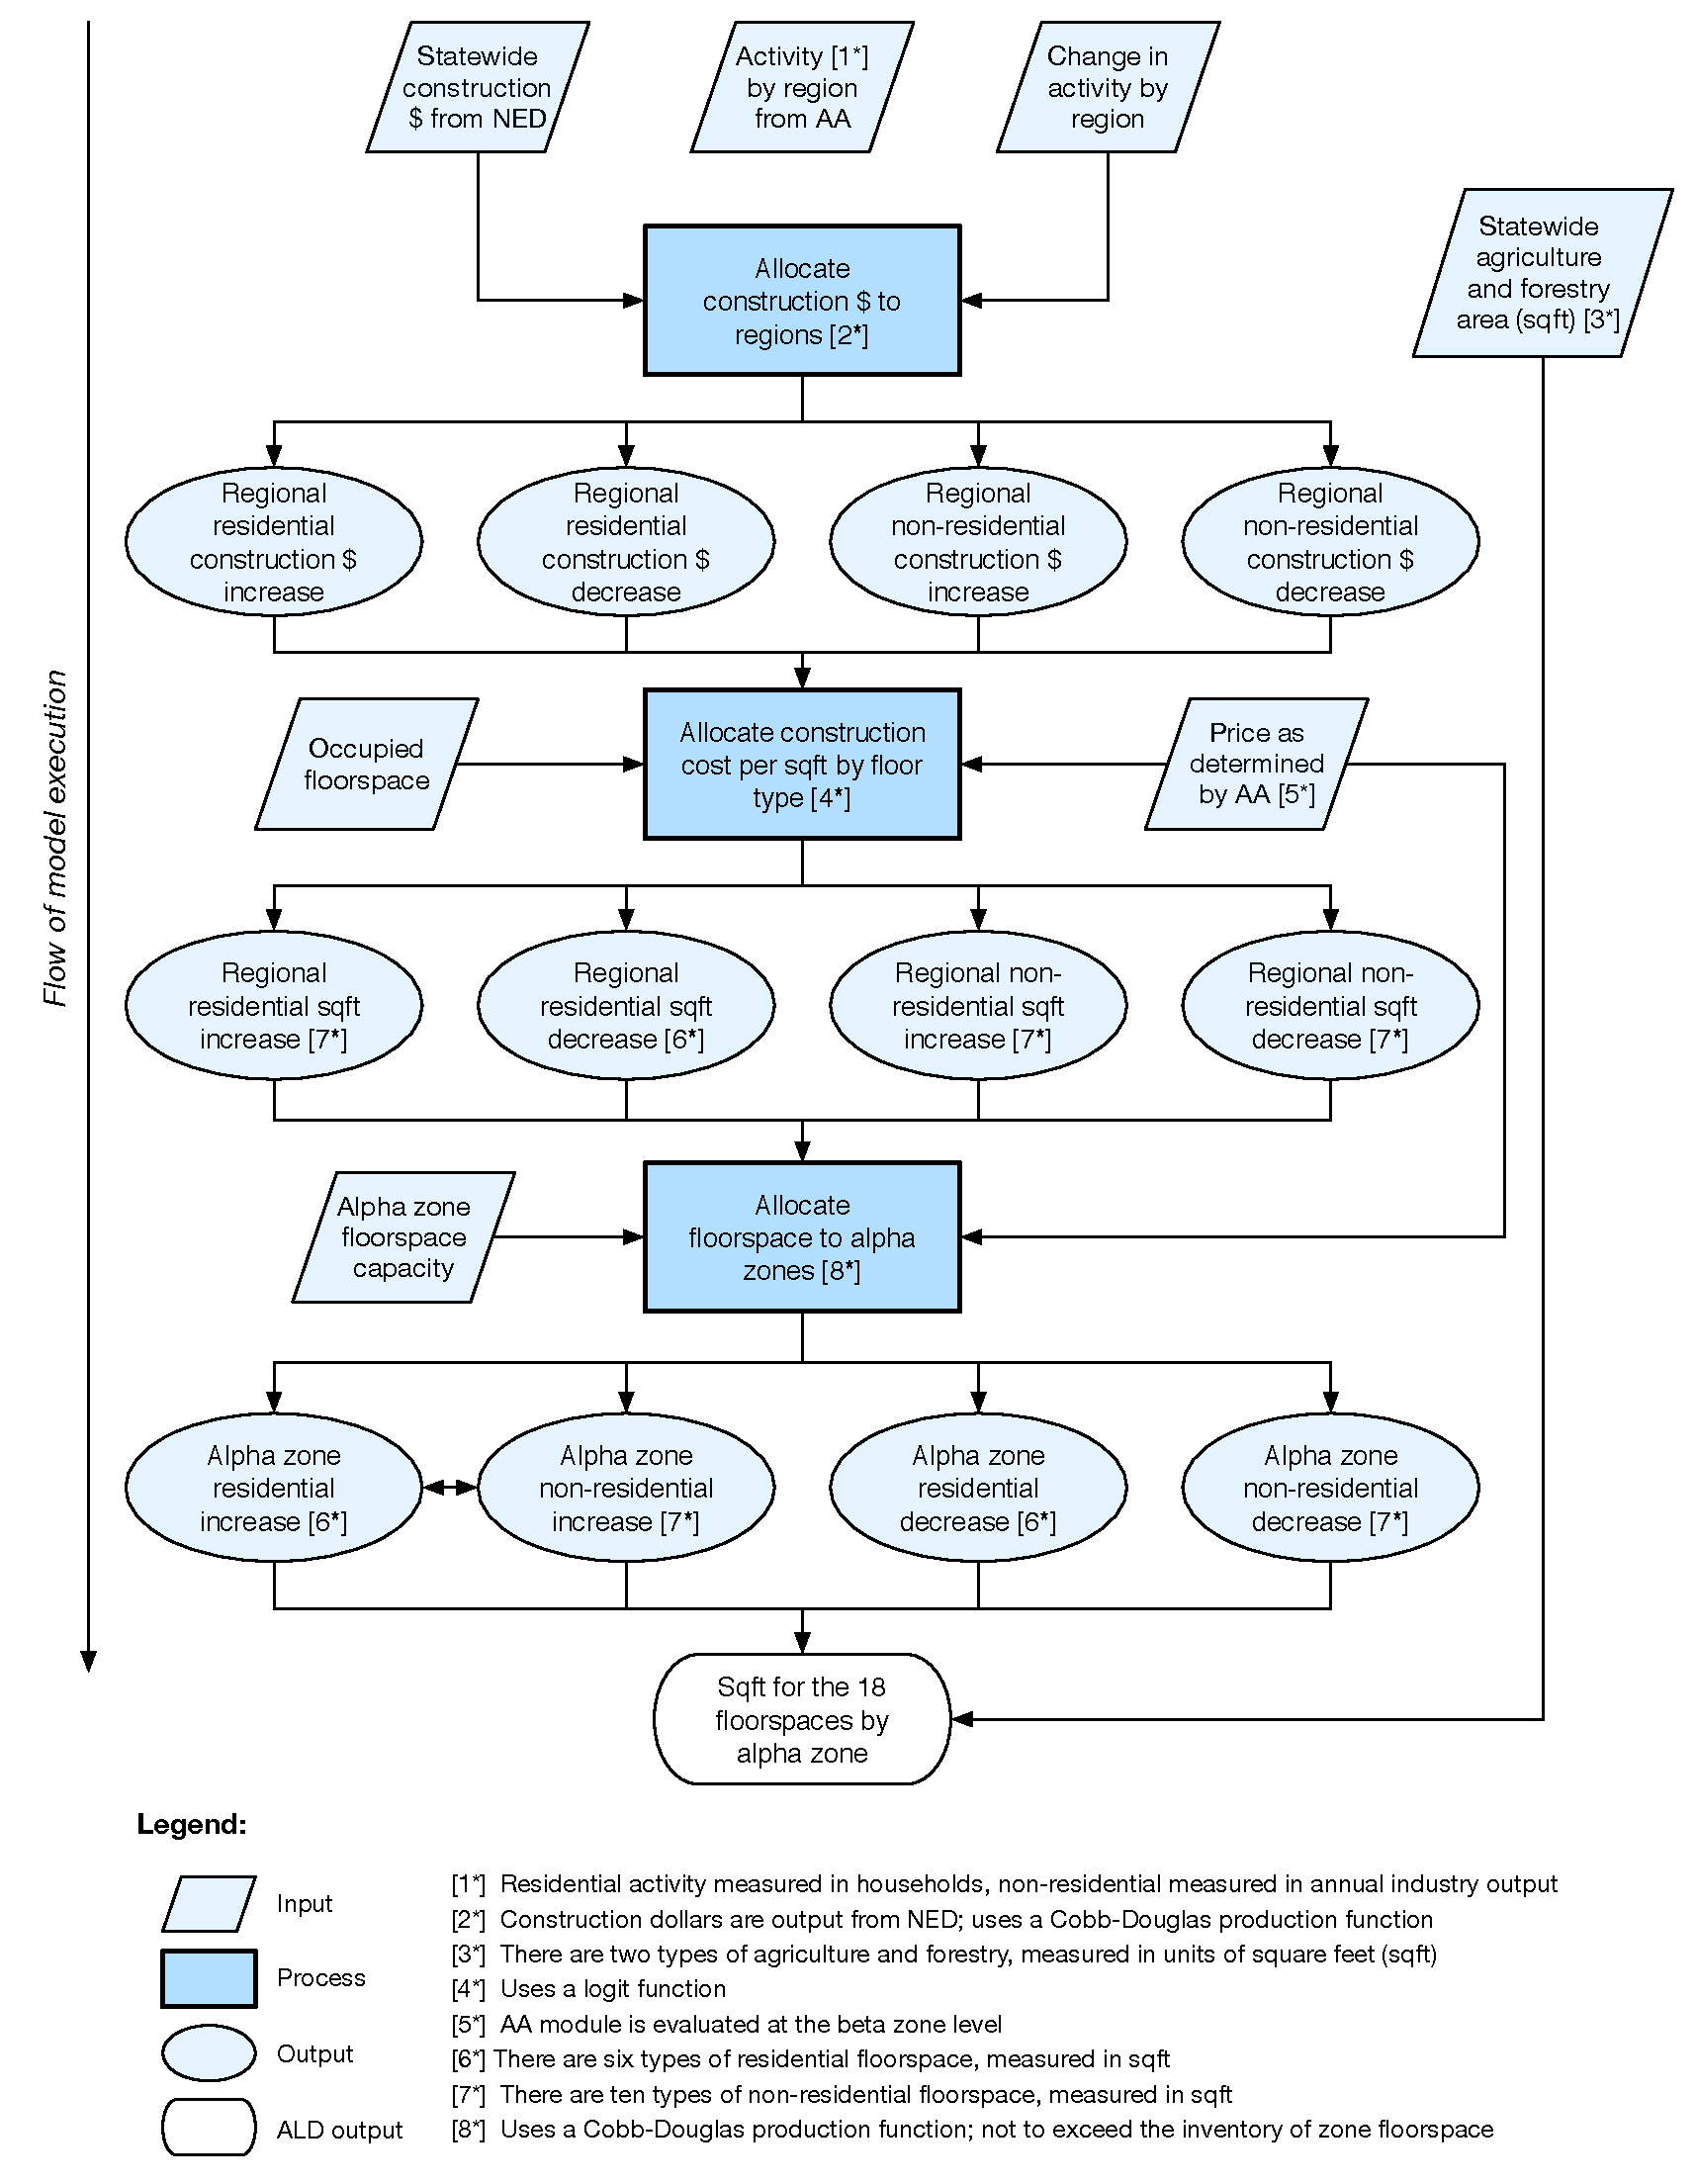
\includegraphics[width=6.5in]{ald/ald-alt-flowchart}
\caption{ALD model components flowchart}\label{fig:ald-components}
\end{figure}

\begin{itemize}
\item \textit{Total model-wide dollar values of residential and non-residential floorspace construction are allocated among 15 regions in the model area.} All subsequent allocations among floorspace types and alpha zones are done within each region. Construction dollars are allocated among regions using a Cobb-Douglas formulation where the independent variables are the region proportions of total activity in the previous year and the region proportions of the change in total activity over the previous two years. The model also incorporates region-specific constants. This process is described in more detail in \S\ref{sec:ald-step1}.
\item \textit{Total model-wide decreases in residential and non-residential floorspace (due to demolition or conversion) are estimated and allocated among regions.} The model-wide value of the floorspace demolished or converted is calculated as a fixed proportion of the model-wide value of floorspace constructed. The model-wide decreases are allocated among regions using the same form of Cobb-Douglas production function as used to allocate the construction increases. Region-specific constants are also included. This process is described in more detail in \S\ref{sec:ald-step1}.
\item \textit{The regional increase values are allocated to floorspace categories} using a logit model where the utility is a function of vacancy rates and the previous quantities of floorspace by category. The model includes alternative specific constants for each floorspace type in each region. The allocated construction values by floorspace category are converted to floorspace area increases (square feet) using model-wide average floorspace construction costs. This process is described in more detail in \S\ref{sec:ald-step2}.
\item \textit{The regional floorspace decrease values are allocated to floorspace categories} using a logit model having the same form as the model for allocating regional increase values. The model includes alternative specific constants for each floorspace type in each region. Floorspace value decreases are converted into area measures (square feet) using the model-wide average floorspace construction costs since the decrease values represent the value of the space lost and not the cost of demolition or conversion. This process is described in more detail in \S\ref{sec:ald-step2}.
\item \textit{The regional floorspace decreases by floorspace category are allocated to alpha zones} using a Cobb-Douglas production function where the input variables are the proportion of total regional floorspace of the category in each zone and the price determined by the AA module for that type of floorspace in the corresponding beta zone. The decrease in floorspace in any zone is not allowed to exceed the inventory of floorspace in the zone. This process is described in more detail in \S\ref{sec:ald-step3}.
\item To allocate the region floorspace increases in each category to alpha zones it is necessary to calculate the capacity of each alpha zone for accommodating floorspace of each category. Floorspace capacity is a function of how much land is currently zoned or planned for development by zoning category, the compatibility of each floorspace category with each plan category and the allowable floor area ratio for each floorspace category in each plan category. A logit model is used to set initial proportions of land by zoning category to floorspace categories. Those initial proportions are then balanced to current floorspace demand by alpha zone while adhering to input development constrains of what floorspace types can and cannot be allocated to a given zoning category quantity. Floor area ratios are also used in the balancing process, as the balancing process must convert between land area and floorspace area, floorspace area capacity being what is ultimately used in allocation of floorspace increases by alpha zone and available land area by zoning category being what is input to the model at the alpha zone level. This process is described in more detail in \S\ref{sec:ald-step4}.
\item \textit{Floorspace increases for each region and category are allocated to alpha zones} using a Cobb-Douglas production function where the inputs are the proportion of total regional floorspace of the category in each zone, the price determined by the AA module for that type of floorspace in the corresponding beta zone and the floorspace capacity for the category in each zone. This process is described in more detail in \S\ref{sec:ald-step5}.
\end{itemize}

\subsection{Allocation of Modelwide Construction Dollars into Regional Dollar Value Increases and Decreases}\label{sec:ald-step1}  % 5.3.1
The first function of ALD is to separately allocate dollar-value production of residential and non-residential construction from the NED module for the entire model area among 15 regions in the model area. In addition, since the total value of construction in the entire model area includes the replacement of floorspace that is removed somewhere in the model area as well as net new floorspace, it is necessary to calculate the value of residential and non-residential floorspace decreases and allocate them to the regions as well. 

Construction dollars are allocated among regions using a Cobb-Douglas model where the independent variables are the region proportions of total activity in the previous year and the region proportions of the change in total activity over the previous two years. The equation has the form:
\begin{equation}\label{eq:5.01}  % 5.01
NIVQ_r = NIVQ \cdot \left( CD_r / \sum_r{CD_r} \right)
\end{equation}

\noindent with:
\begin{equation}\label{eq:5.02}   % 5.02
CD_r = (ActProp_r + \beta_{1v})^{\beta_{2v}} \cdot (ActChgProp_r + \beta_{3v})^{\beta_{4v}} \cdot A_{scr}
\end{equation}

\noindent where:
\begin{align*}
NIVQ &= \text{modelwide total residential (nonresidential) construction value by year from NED} \\
 &~~~~~\text{(construction\_forecast.csv)} \\
NIVQ_r &= \text{residential (nonresidential) construction value for region $r$} \\
CD_r &= \text{Cobb-Douglas production function for region $r$ (estimated)} \\
ActProp_r &= \text{proportion of total modelwide residential (nonresidential) activity occurring in} \\
 &~~~~~\text{region $r$ (see notes below)} \\
ActChgProp_r &= \text{proportion of total modelwide residential (nonresidential) activity change} \\
 &~~~~~\text{occurring in region $r$ (see notes below)} \\
\beta_{*v} &= \text{coefficients estimated separately for residential and nonresidential construction} \\
 &~~~~~\text{(estimated)} \\
Asc_r &= \text{alternative specific constant for region estimated separately for residential} \\
 &~~~~~\text{and nonresidential construction (adjusted)}
\end{align*}

\noindent Decreases in the value of floorspace are calculated from the modelwide construction total are allocated to regions as follows:
\begin{equation}\label{eq:5.03}  % 5.03
NDVQ_r = D_f \cdot NIVQ \cdot \left( CD_r / \sum_r{CD_r} \right)
\end{equation}

\noindent with:
\begin{equation}  % 5.04
CD_r = (ActProp_r + \beta_{5v})^{\beta_{6v}} \cdot (ActChgProp_r + \beta_{7v})^{\beta_{8v}} \cdot A_{scr}
\end{equation}

\noindent where $D_f$ modelwide proportion of residential (nonresidential) floorspace construction value, and the other variables are defined as described above.

The measure of activity used to calculate the proportions of total activity and the proportions of activity change is measured using the ``quantity'' output from the AA module. This is households, in the case of residential activities and annual output in 2009 dollars, in the case of non-residential activities (from AA ExchangeResults.csv prior year output aggregated to ALD regions).

The proportion of activity change is calculated after the regional activity change values are rescaled by subtracting the minimum regional value from all regional values. The rescaling is necessary to assure that the activity change proportions are in the range of 0 to 1. For the first two simulation years, when there is no computable activity change, it is assumed that all regions have an equal proportion of the activity change.


\subsection{Allocation of Regional Dollar Increases and Decreases into Floorspace Types}\label{sec:ald-step2}   % 5.3.2
Regional residential and non-residential floorspace construction and decreases are allocated separately to the floorspace categories using a logit model with utility functions that include regional vacancy rates by floorspace category and proportions of previous year floorspace value in each floorspace category. In calibration, the second term in equation \ref{eq:5.06} was modified from the construction cost value, to the AA value (based on prior year AA floorspace prices). Thus, this term serves not only as a size measure, but also as a signal for which floorspace types are in demand (indicated by higher prices), which helps to allocate construction dollars more effectively. The logit model for floorspace construction has the form:
\begin{equation}\label{eq:5.05}   % 5.05
NIVQ_{f,r} = NIVQ_r \cdot exp(\lambda_{q1} \cdot U_{f,r}) / \sum_f exp(\lambda_{q1} \cdot U_{f,r})
\end{equation}
\noindent with:
\begin{equation}  % 5.06
U_{f,r} = {\beta_{q1,f}} \cdot VacRate_{f,r} + {\beta_{q2}} \cdot ln \left( TVQ_{f,r} / \sum_f TVQ_{f,r} \right) + ASC_{f,r}
\label{eq:5.06}
\end{equation}

\noindent where:
\begin{align*}
NIVQ_{f,r} &= \text{value of floorspace construction allocated to category $f$ in region $r$} \\
NIVQ_r &= \text{total value of floorspace construction in region $r$ (equation \ref{eq:5.01})} \\
U_{f,r} &= \text{utility of floorspace category $f$ in region $r$} \\
\lambda_{q1} &= \text{dispersion parameter of the logit model (estimated separately for residential} \\
 &~~~~~\text{and non-residential floorspace construction)} \\
VacRate_{f,r} &= \text{average vacancy rate for floorspace category $f$ in region $r$ in the} \\
 &~~~~~\text{previous year (calculated from AA ExchangeResults.csv occupied space use and} \\
 &~~~~~\text{ALD FloorspaceInventory.csv total space inventory)} \\
TVQ_{f,r} &= \text{dollar value of floorspace category $f$ in region $r$ in the previous year} \\
 &~~~~~\text{(calculated from ALD FloorspaceInventory.csv floorspace inventory and} \\
 &~~~~~\text{AA ExchangeResults.csv module square foot values of floorspace summed to} \\
 &~~~~~\text{floorspace category)} \\
\beta_{q1,f} &= \text{coefficient estimated separately for residential and non-residential} \\
 &~~~~~\text{construction (estimated)} \\
\beta_{q2} &= \text{sensitivity coefficient for the previous year zone proportion of total} \\
 &~~~~~\text{floorspace of this type (estimated)} \\
ASC_{f,r} &= \text{alternative specific constant for construction of floorspace category $f$ in} \\
 &~~~~~\text{region $r$ (estimated)}
\end{align*}

\noindent The logit model for floorspace decreases has the form:
\begin{equation}\label{eq:5.07}   % 5.07
NDVQ_{f,r} = NDVQ_r \cdot a \left[ exp({\lambda_{q2}} \cdot U_{f,r}) / \sum_f exp({\lambda_q} \cdot U_{f,r}) \right]
\end{equation}
\noindent with:
\begin{equation}   % 5.08
U_{f,r} = {\beta_{q3,f}} \cdot VacRate_{f,r} + \beta_{q4} \cdot ln \left( TVQ_{f,r} / \sum_f TVQ_{f,r} \right) + ASC_{f,r}
\end{equation}

\noindent where:
\allowdisplaybreaks
\begin{align*}
NDVQ_{f,r} &= \text{value of floorspace decrease allocated to category $f$ in region $r$} \\
NDVQ_r &= \text{total value of floorspace decrease in region (equation \ref{eq:5.03})} \\
U_{f,r} &= \text{utility of floorspace category $f$ in region $r$} \\
\beta_{q2} &= \text{dispersion parameter of the logit model estimated separately for residential} \\
 &~~~~~\text{and non-residential floorspace construction (estimated)} \\
VacRate_{f,r} &= \text{average vacancy rate for floorspace category $f$ in region $r$ in the previous} \\
 &~~~~~\text{year (calculated from AA ExchangeResults.csv occupied space use and ALD} \\
 &~~~~~\text{FloorspaceInventory.csv total space inventory)} \\
TVQ_{f,r} &= \text{dollar value of floorspace category $f$ in region $r$ in previous year (calculated from} \\
 &~~~~~\text{ALD FloorspaceInventory.csv floorspace inventory and AA ExchangeResults.csv} \\
 &~~~~~\text{square foot values of floorspace summed to floorspace category)} \\
\beta_{q3,f} &= \text{coefficient estimated separately for residential and non-residential construction} \\
 &~~~~~\text{(estimated)} \\
\beta_{q4} &= \text{sensitivity coefficient for the previous year zone proportion of total floorspace} \\
 &~~~~~\text{of this type (estimated)} \\
ASC_{f,r} &= \text{alternative specific constant for decrease in floorspace category $f$ in region $r$} \\
 &~~~~~\text{(estimated)}
\end{align*}

\noindent The regional average vacancy rate for a given category of floorspace is calculated as follows:
\begin{equation}   % 5.09
VacancyRate_{f,r} = \left( \sum_{\alpha,r} PrevQ_{f,\alpha,r} - \sum_{\beta,r} Occupied_{f,\beta,r} \right) / \sum_{\alpha,r} PrevQ_{f,\alpha,r}
\end{equation}

\noindent where:
\begin{align*}
\alpha &= \text{index representing alpha zones in region $r$} \\
\beta &= \text{index representing betazones in region $r$} \\
PrevQ_{f,\alpha,r} &= \text{building area-based quantity of total floorspace of category $f$ in zone $\alpha$} \\
 &~~~~~\text{of region $r$ in the previous year (ALD previous year FloorspaceInventory.csv by} \\
 &~~~~~\text{alpha zone)} \\
Occupied_{f,\beta,r} &= \text{building area-based quantity of occupied floorspace of category $f$ in zone} \\
 &~~~~~\text{$\beta$ of region $r$ in the previous year (AA ExchangeResults.csv by beta zone)}
\end{align*}

The dollar-value quantity of floorspace in each category $f$ in each region is converted into an equivalent area-based quantity (in building sqft) using modelwide average unit construction costs (per building sqft) specified exogenously. It is calculated as follows:
\begin{equation}\label{eq:5.10}  % 5.10
NIQ_{f,r} = NIVQ_{f,r} / ConstrCost_f
\end{equation}
\begin{equation}\label{eq:5.11}  % 5.11
NDQ_{f,r} = NDVQ_{f,r} / ConstrCost_f
\end{equation}

\noindent where:
\begin{align*}
NIQ_{f,r} &= \text{building area-based quantity of floorspace construction allocated to category $f$ in} \\
 &~~~~~\text{region $r$} \\
NIVQ_{f,r} &= \text{value of floorspace construction allocated to category $f$ in region $r$ (equation \ref{eq:5.05})} \\
NDQ_{f,r} &= \text{building area-based quantity of floorspace decrease allocated to category $f$ in} \\
 &~~~~~\text{region $r$} \\
NDVQ_{f,r} &= \text{value of floorspace decrease allocated to category $f$ in region $r$ (equation \ref{eq:5.07})} \\
ConstrCost_f &= \text{modelwide average unit construction costs for floorspace category $f$ (exogenous} \\
 &~~~~~\text{ConstructionCosts.csv)}
\end{align*}

\subsection{Allocation of Zonal Floorspace Decrease}\label{sec:ald-step3}   % 5.3.3
Regional decreases in the quantity of floorspace in each category are allocated among alpha zones in each region using a Cobb-Douglas model where the input variables are the proportion of total regional floorspace of the category in each zone and the price determined by the AA module for that type of floorspace in the corresponding beta zone. The equations for this model are as follows:
\begin{equation}\label{eq:5.12}  % 5.12
DQ_{f,\alpha,r} = NDQ_{f,r} \cdot (CD_{f,\alpha,r}) / \sum_\alpha{CD_{f,\alpha,r}}
\end{equation}

\noindent with:
\begin{equation}   % 5.13
CD_{f,\alpha,r} = (PrevProp_{f,\alpha,r})^{\beta_{3f}} \cdot (Price_{f,\alpha,r})^{\beta_{4f}}
\end{equation}
\noindent where:
\begin{align*}
\alpha &= \text{index representing a specific alpha zone} \\
DQ_{f,\alpha,r} &= \text{decrease in quantity of floorspace category $f$ in alpha zone $\alpha$ in region $r$} \\
NDQ_{f,r} &= \text{building area-based quantity of floorspace decrease allocated to category $f$ in} \\
 &~~~~~\text{region $r$ (equation \ref{eq:5.11})} \\
CD_{f,\alpha,r} &= \text{Cobb-Douglas production function for floorspace category $f$ in alpha zone $\alpha$} \\
 &~~~~~\text{in region $r$ (estimated)} \\
PrevProp_{f,\alpha,r} &= \text{share of previous year regional floorspace quantity of category $f$ in alpha} \\
 &~~~~~\text{zone $\alpha$ (using ALD previous year FloorspaceInventory.csv)} \\
Price_{f,\alpha,r} &= \text{previous year price of floorspace quantity of category $f$ in the beta zone in} \\
 &~~~~~\text{which alpha zone $\alpha$ is located (previous year AA ExchangeResults.csv)} \\
\beta_{3f}, \beta_{4f} &= \text{allocation coefficients (estimated separately for residential and non-residential} \\
 &~~~~~\text{decreases)}
\end{align*}

\subsection{Land Capacity Calculation}\label{sec:ald-step4}   % 5.3.4
To allocate the region floorspace increases in each category to alpha zones it is first necessary to calculate the capacity of each alpha zone for accommodating floorspace of each category. Floorspace capacity is a function of how much land is currently zoned or planned for development by plan category, the compatibility of each floorspace category with each zoning category and the allowable floor area ratio for each floorspace category in each zoning category. The following logit model is used to set initial proportions of land by zoning category to floorspace categories:
\begin{equation}\label{eq:5.14}   % 5.14
LandProp_{f,z} = exp(U_{f,z}) / \sum_f exp(U_{f,z})
\end{equation}
\noindent with:
\begin{equation}\label{eq:5.15}   % 5.15
U_{f,z} = \lambda_p \left[ stc \cdot ln(LandSQFT_f) + ln(Compat_{f,z}) \right]
\end{equation}
\noindent subject to the constraint $exp(U_{f,z}) \ge 0$, and where:
\begin{align*}
LandProp_{f,z} &= \text{proportion of zoning category $z$ land area allocated to floorspace type $f$} \\
U_{f,z} &= \text{utility of allocating land in zoning code $z$ to floorspace type $f$} \\
Compat_{f,z} &= \text{compatibility of floorspace type $f$ in zoning category $z$ (exogenous,} \\
 &~~~~~\text{zoning\_compatibility.csv)} \\
stc &= \text{parameter for the sensitivity to the size term (estimated)} \\
\lambda_{p} &= \text{dispersion parameter for the sensitivity to input compatibility matrix (estimated)} \\
LandSQFT_f &= \text{baseyear modelwide land area devoted to each floorspace type (exogenous,} \\
 &~~~~~\text{LandSQFTxFLR.csv, which comes from inputs stored in Visum, SI)}
\end{align*}

The land area capacities for each floorspace category in each alpha zone are initially calculated from the proportional allocation of zoning categories to floorspace categories, the inventory of zoning by type and alpha zone and maximum floor area ratios by zoning type and floorspace category as follows:
\begin{equation}\label{eq:5.16}    % 5.16
LandCap_{z,f,\alpha} = LandProp_{f,z} \cdot ZoneArea_{z,\alpha}
\end{equation}
\noindent where:
\begin{align*}
LandCap_{z,f,\alpha} &= \text{land area capacity for zoning category and floorspace category $f$ in alpha zone $\alpha$} \\
LandProp_{f,z} &= \text{proportion of zoning category $z$ land area allocated to floorspace type $f$} \\
 &~~~~~\text{(equation \ref{eq:5.14})} \\
ZoneArea_{z,\alpha} &= \text{land area with zoning category $z$ in alpha zone $\alpha$ (exogenous,} \\
 &~~~~~\text{LandSQFTxZoning.csv, which is output from inputs stored in Visum, SI)}
\end{align*}

The initial land area capacities calculated in equation \ref{eq:5.15} are informed by zoning compatibility, but not by demand. These initial capacities, for example, may create a 50/50 capacity split of warehouse and light industrial for a given zone, but in this example the zoning allows for the area to be one hundred percent filled with either light industrial or warehouse. Without adjusting to demand, the given zone might have a demand for ten percent light industrial and ninety percent warehouse, but because the 50/50 split has been set to capacity the development of warehouse space in that area would be artificially constrained.  

Therefore, a multi-dimensional balancing method is applied that respects the hard constraints of total land capacity by alpha zone, zoning compatibility between zoning category and floorspace categories, and total buildable floorspace by alpha zone. The balancing process starts with the initial land area capacities calculated in equation \ref{eq:5.16} as the initial seed to be balanced. The land square footage across zoning and floorspace categories are summed to alpha zone to create a total buildable land area by alpha zone.  Next initial floorspace capacity proportions are calculated by multiplying the land area capacities calculated in equation \ref{eq:5.16} by the maximum floor area ratios by zoning type and floorspace category as follows:
\begin{equation}\label{eq:5.17}    % 5.17
FloorProp_{z,f,\alpha} = FloorCap_{z,f,\alpha} / \sum_{z,f} FloorCap_{z,f,\alpha}
\end{equation}
\noindent with: 
\begin{equation}    % 5.18
FloorCap_{z,f,\alpha} = LandCap_{z,f,\alpha} \cdot FAR_{f,z}
\end{equation}
\noindent where:
\begin{align*}
FloorProp_{z,f,\alpha} &= \text{proportion of available floorspace for each zoning category in alpha zone $\alpha$} \\
 &~~~~~\text{and floorspace category $f$} \\
FloorCap_{z,f,\alpha} &= \text{floorspace capacity for zoning category and floorspace category $f$ in alpha} \\
 &~~~~~\text{zone $\alpha$} \\
LandCap_{z,f,\alpha} &= \text{land area capacity for zoning category and floorspace category $f$ in alpha} \\
 &~~~~~\text{zone $\alpha$ (equation \ref{eq:5.16})} \\
FAR_{f,z} &= \text{maximum floor-to-area ratio for floorspace category $f$ in zoning categories $z$} \\
 &~~~~~\text{(exogenous, far.csv)}
\end{align*}

\noindent The demand for floorspace in each zone by zoning category is then determined as follows:
\begin{equation}\label{eq:5.19}   % 5.19
Demand_{z,f,\alpha} = FloorProp_{z,f,\alpha} \cdot Quant_{f,\alpha}
\end{equation}
\noindent where:
\begin{align*}
Demand_{z,f,\alpha} &= \text{pervious year floorspace quantity proportioned to zoning categories $z$ by} \\
 &~~~~~\text{floorspace type $f$ for each alpha zone $\alpha$} \\
FloorProp_{z,f,\alpha} &= \text{proportion of available floorspace for each zoning category in alpha zone $\alpha$} \\
 &~~~~~\text{and floorspace category $f$ (equation \ref{eq:5.17})} \\
Quant_{f,\alpha} &= \text{previous year floorspace quantity of category $f$ in alpha zone $\alpha$ (using ALD} \\
 &~~~~~\text{previous year FloorspaceInventory.csv)}
\end{align*}

From the products of equations \ref{eq:5.16} and \ref{eq:5.19} several dimensional control totals are formed. The total available land space for each zone is summed from $LandCap_{z,f,\alpha}$ (Equation \ref{eq:5.16}). The total quantity of floorspace by ALD region and floorspace type are summed from $Demand_{z,f,\alpha}$ (equation \ref{eq:5.19}). Then a custom two-dimensional balancing process is applied that ensures that all land space for a given zone is allocated within allowed zoning compatibility by floorspace type ($Compat_{f,z}$) and that total demand for each floorspace type by ALD region is satisfied.

The custom aspect of this balancing process is a switch between floorspace and land space between the two dimensions (since one control is on total land space and another is on total floorspace). The switching between those dimensions is done using the $FAR_{f,z}$ input, which is embedded in the balancing steps to convert between floorspace and land space for each floorspace type and zoning category. In the end overall available land space is fully allocated to floorspace types based on regional demand, and at an ALD region level the process ensures that there is enough floorspace for each type within each region.\footnote{Note that the model currently has a fatal error if a floorspace type runs out of space within an ALD region. This is much different than a specific zone running out of space. Many zones run out of space, but the ALD regions are defined by multiple counties. It is a safe assumption that a multi-county area should be able to find some amount of floorspace for all floorspace types to meet demand. Running out of space at a regional level indicates that a multi-county area is built to full capacity across all zones within that multi-county area.}


\subsection{Allocation of Zonal Floorspace Increase}\label{sec:ald-step5}    % 5.3.5
The regional floorspace construction quantities are allocated to alpha zones. These allocated quantities are then added to the updated floorspace inventory after decreases have been apportioned to yield the new floorspace qualities by alpha zone. A Cobb-Douglas model is used to allocate the construction among the alpha zones as follows:
\begin{equation}    % 5.20
IQ_{f,\alpha,r} = NIQ_{f,r} \left[ CD_{f,\alpha,r} / \sum_{\alpha,r} CD_{f,\alpha,r} \right]
\end{equation}
\noindent with:
\begin{equation}   % 5.21
CD_{f,\alpha,r} = (PrevProp_{f,\alpha,r} + \beta_{9f})^{\beta_{5f}} \cdot (Price_{f,\alpha,r})^{\beta_{6f}} \cdot \left[ 1 -\beta_{7f} \cdot (Quant_{f,\alpha,r} / Cap_{f,\alpha,r})^{\beta_{8f}} \right]
\end{equation}
\noindent with the constraints that $PrevDQ_{f,\alpha,r} \ge 0$ and $Cap_{f,\alpha,r} \ge PrevQ_{f,\alpha,r}$, and where:
\begin{align*}
\alpha &= \text{index representing a specific alpha zone} \\
IQ_{f,\alpha,r} &= \text{increase in quantity of floorspace category $f$ in alpha zone $\alpha$ in region $r$} \\
NIQ_{f,r} &= \text{building area-based quantity of floorspace construction allocated to category $f$} \\
 &~~~~~\text{in region $r$ (equation \ref{eq:5.10})} \\
CD_{f,\alpha,r} &= \text{Cobb-Douglas production function for floorspace category $f$ in alpha zone $\alpha$ in} \\
 &~~~~~\text{region $r$ (estimated)} \\
PrevProp_{f,\alpha,r} &= \text{share of previous year region $r$ floorspace quantity of category $f$ in alpha zone} \\
 &~~~~~\text{$\alpha$ (using ALD previous year FloorspaceInventory.csv)} \\
Price_{f,\alpha,r} &= \text{previous year price of floorspace quantity of category $f$ in the beta zone in} \\
 &~~~~~\text{which alpha zone $\alpha$ is located (AA previous year ExchangeResults.csv)} \\
Quant_{f,\alpha,r} &= \text{previous year region $r$ floorspace quantity of category $f$ in alpha zone $\alpha$ (using} \\
 &~~~~~\text{ALD previous year FloorspaceInventory.csv)} \\
Cap_{f,\alpha,r} &= \text{building area capacity for floorspace category $f$ in alpha zone $\alpha$ (see \S\ref{sec:ald-step4})} \\
\beta_{*f} &= \text{coefficients (estimated separately for residential and non-residential decreases)}
\end{align*}

After this allocation of increases in floorspace, the resulting new quantities in each zone are determined, as follows:
\begin{equation}   % 5.22
CurrQ_{f,\alpha,r} = PrevDQ_{f,\alpha,r} + IQ_{f,\alpha,r}
\end{equation}
\noindent with:
\begin{equation}  % 5.23
PrevDQ_{f,\alpha,r} = PrevQ_{f,\alpha,r} - DQ_{f,\alpha,r}
\end{equation}
\noindent where:
\begin{align*}
CurrQ_{f,\alpha,r} &= \text{the area-based quantity of floorspace category $f$ in zone $i$ in the current year} \\
PrevDQ_{f,\alpha,r} &= \text{updated quantity of floorspace category $f$ in alpha zone $\alpha$ in region $r$} \\
 &~~~~~\text{after the decreases are taken into account} \\
PrevQ_{f,\alpha,r} &= \text{building area-based quantity of total floorspace of category $f$ in zone $\alpha$ of} \\
 &~~~~~\text{region $r$ in the previous year (ALD previous year FloorspaceInventory.csv by} \\
 &~~~~~\text{alpha zone)} \\
DQ_{f,\alpha,r} &= \text{decrease in quantity of floorspace category $f$ in alpha zone $\alpha$ in region $r$} \\
 &~~~~~\text{(equation \ref{eq:5.12})}
\end{align*}

\subsection{Completing the Floorspace Inventory}\label{sec:ald-completing-inventory}   % 5.3.6
ALD produces an output file identifying the total floorspace by floorspace type and alpha zone. Total floorspace includes the residential and non-residential components discussed above. Productive land sqft of agricultural and logging lands are added to total floorspace in each alpha zone. In the future, after-market additions to floorspace could also be added at this point, as user inputs. 

\subsection{Agriculture and Logging Lands}
For the Oregon Statewide Integrated Model, productive agriculture and logging lands are assumed to be fixed in quantity and location (AgForestFloorspace.csv). ALD initially strips the agriculture and logging lands from the previous year floorspace input and adds these same quantities back onto the new residential/nonresidential floorspace inventory before producing the current year floorspace output. It should be noted that these categories are in units of land sqft, not building-area based sqft as in other floorspace types. 

Additionally, AA requires a consistent use of floorspace per employee per year in a given industry (see Section \ref{sec:aa-floorspace-quantities} on page \pageref{sec:aa-floorspace-quantities}). Thus, an AA version of the agriculture and logging lands was developed for the base year, and held constant in all future years. 

In the future, it is anticipated that ALD could be modified rather easily to allow agriculture and logging lands to be created directly from the zoning coverage. Thus if in future years the area covered by agriculture and logging zoning categories decreased, so would the available lands, which would in turn affect the amount of agriculture and logging production activity when used into the AA module. 

\section{Software Implementation}
ALD is implemented in the R statistical programming language, and called using R CMD BATCH from Java. % [8]?
The work was started in the R language because some of the operations were drawn from R work used in the first generation, SWIM1 model. The use of R also facilitated the use of evolutionary algorithms to estimate the model coefficients.

Three scripts are required to run the ALD module: ALD.R, ALD\_Inputs.R and ALD\_Functions.R. ALD.R is the main script which calls the other two scripts and steps through the ALD process. The main program, ALD.R, calls ALD\_inputs.R. ALD.R is split into five main sections. The first section parses the arguments to R CMD BATCH and identifies the locations of the code and data directories, and builds the names of the directory paths. 

The second section calls the ALD\_Functions.R script which defines a number of functions which carry out the different portions of the ALD model described above. The main functions are:
\begin{itemize}
\item allocateConstToRegions
\item allocateDecreaseToRegions
\item allocateFloorProd
\item allocateFloorDecrease
\item calcFloorCapacity
\item calculateFloorDecrease
\item allocateIncrease
\end{itemize}

\noindent The notation used in the code closely follows the notation in the equations documented in \S\ref{sec:aa-component-models}. The variable names are similar to the variable names in the equations. The dimensionality of variables is noted using a special ``dot'' notation. For example, $PrevProp_{f,\alpha,r}$ is notated as $PrevProp.AxFx$.

Abbreviations for the dimensions follow the period in the variable name. In this case, the object is a matrix where the rows refer to alpha zones (Ax) in region X and the columns refer to floorspace category X (Fx) (either residential or non-residential). 

The third section calls the ALD\_Inputs.R script which identifies the input data file names, the model coefficients files and then loads the data and coefficients. The fourth section performs all of the ALD module calculations and creates all of the output data objects.

The last section writes out all of the results of the calculation of floorspace quantities that are used by AA in the current year and used by ALD in the following year. In addition, a number of files are written out to help in the diagnosis of ALD outputs. Furthermore the R workspace is saved so that the state of all the variables in the ALD simulation can be examined.

At the close of the module, a ``complete'' message is returned to the model run process.

\section{S1 and S2 Module Parameters}
Most of the ALD module parameters are S2 parameters which were calibrated through a parameter search process used to find the best fit. Two of the parameters, however, are S1 parameters which were calculated directly from calibration data:
\begin{itemize}
\item Modelwide floorspace unit construction costs by floorspace category (ConstructionCost.csv) discussed in \S\ref{sec:ald-unit-cost-rates}.
\item Modelwide residential and non-residential floorspace value decrease factors (Df) discussed in \S\ref{sec:ald-floorspace-decrease-factors}.
\end{itemize}

The target data used in calibrating all the ALD sub-models are 1990-2000 annual net change in county building stock (sqft) by floorspace type, purchased from McGraw-Hill FWDodge. This data and its preparation for use in model calibration is discussed in \S\ref{sec:ald-baseyear-floorspace}.

The calibration of S2 parameters was challenging because of the relative complexity of the model and data limitations. Calibration of ALD requires the estimation of 76 parameters and 34 alternative specific constants. These include the parameters and alternative specific constants for both the decrease and increase functions. The floorspace data though, only provide observations for net changes in floorspace. They do not provide separate observations for floorspace decreases and increases. Because of the large number of parameters and the lack of observed data on decreases and increases, the estimation process was split into steps and an automated search process using evolutionary algorithms was used for estimating parameters for three of the steps. The steps are as follows:
\begin{itemize}
\item Calibration of land capacity model parameters (\S\ref{sec:ald-capacity-parameters}).
\item Calibration of model parameters for allocating modelwide construction dollars into regional dollar value increases and decreases (\S\ref{sec:ald-increase-decrease}).
\item Calibration of model parameters for allocating regional dollar increases and decreases into floorspace types (\S\ref{sec:ald-allocate-inc-dec}).
\item Calibration of model parameters for allocating regional floorspace decreases and increases to alpha zones (\S\ref{sec:ald-inc-dec-alpha}).
\end{itemize}

A parameter search process using evolutionary algorithms was applied in the last three steps. Although there are differences in how an evolutionary algorithm was applied to each step, the basic approach is the same and incorporates the following elements:
\begin{itemize}
\item The algorithm starts with a set of 1000--2000 parameter combinations that are established by random draws from pre-established parameter ranges.
\item The algorithm iterates through a number of evolutionary cycles. The number of cycles is established in order that model results converge to calibration target values. 
\end{itemize}

\noindent The following procedures are carried out in each cycle:
\begin{itemize}
\item The model is run for each parameter combination and the goodness of fit of the result with calibration targets is calculated.
\item The best-fitting parameter combinations are identified and retained for the next cycle. The number that is retained is gradually reduced through the cycles to force convergence on a solution (e.g. first retaining 100 for several cycles, then 75, then 50 and then 25).
\item Additional combinations are added to the ones that are retained to expand the set back to its original size. These additional combinations are generated from the retained combinations by recombining parameters from randomly selected combinations and by choosing new values randomly from within the range of values of the retained combinations.
\end{itemize}

\noindent This evolutionary algorithm approach has worked successfully for estimating the ALD parameters. More details of the calibration steps and results follow, with more detail in \cite{weidner07}. % Reference 38 in v30

\subsection{Unit Construction Cost Rates}\label{sec:ald-unit-cost-rates}  % 5.5.1
Unit costs for construction were developed from FWDodge Construction starts database reflecting actual construction in the 75-county study area between 1990 and 2002. Construction costs were converted into 1990 constant dollars using USGSP deflators. Study area averages (\$/sqft in 1990 dollars) were estimated by dividing total construction, demolition and clean-up costs incurred, by the increase in space (sqft). Table \ref{tab:building-space-mapping} identifies how the FWDodge space categories were mapped to the model floorspace types (note that this work was done to previous floorspace types which mapped to PI). The weighting is based on available space of each type within the study area. Figure \ref{fig:average-construction-costs} identifies the resulting unit construction cost rates for new constructions (NEW), space additions (ADD) and the significantly higher cost alteration of space (ALT). An average of the NEW and ADD space categories, weighted by the type of space added over the ten-year period, also shown in Figure \ref{fig:average-construction-costs}, were used as input to ALD and are stored in ConstructionCosts.csv in the ``inputs/parameters'' folder. When AA was implemented these values were converted from 1990 to 2009 dollars by multiplying by 1.518 (obtained from USGSP deflators). Additionally, the Depot and Warehouse floorspace categories were collapsed to just Warehouse in AA, so a weighted average of the construction costs for Depot and Warehouse was calculated and used for the new Warehouse value.
  
\begin{sidewaystable}  % Table 5-2
\centering
\caption{Mapping FWDodge to SWIM2 building space types}\label{tab:building-space-mapping}
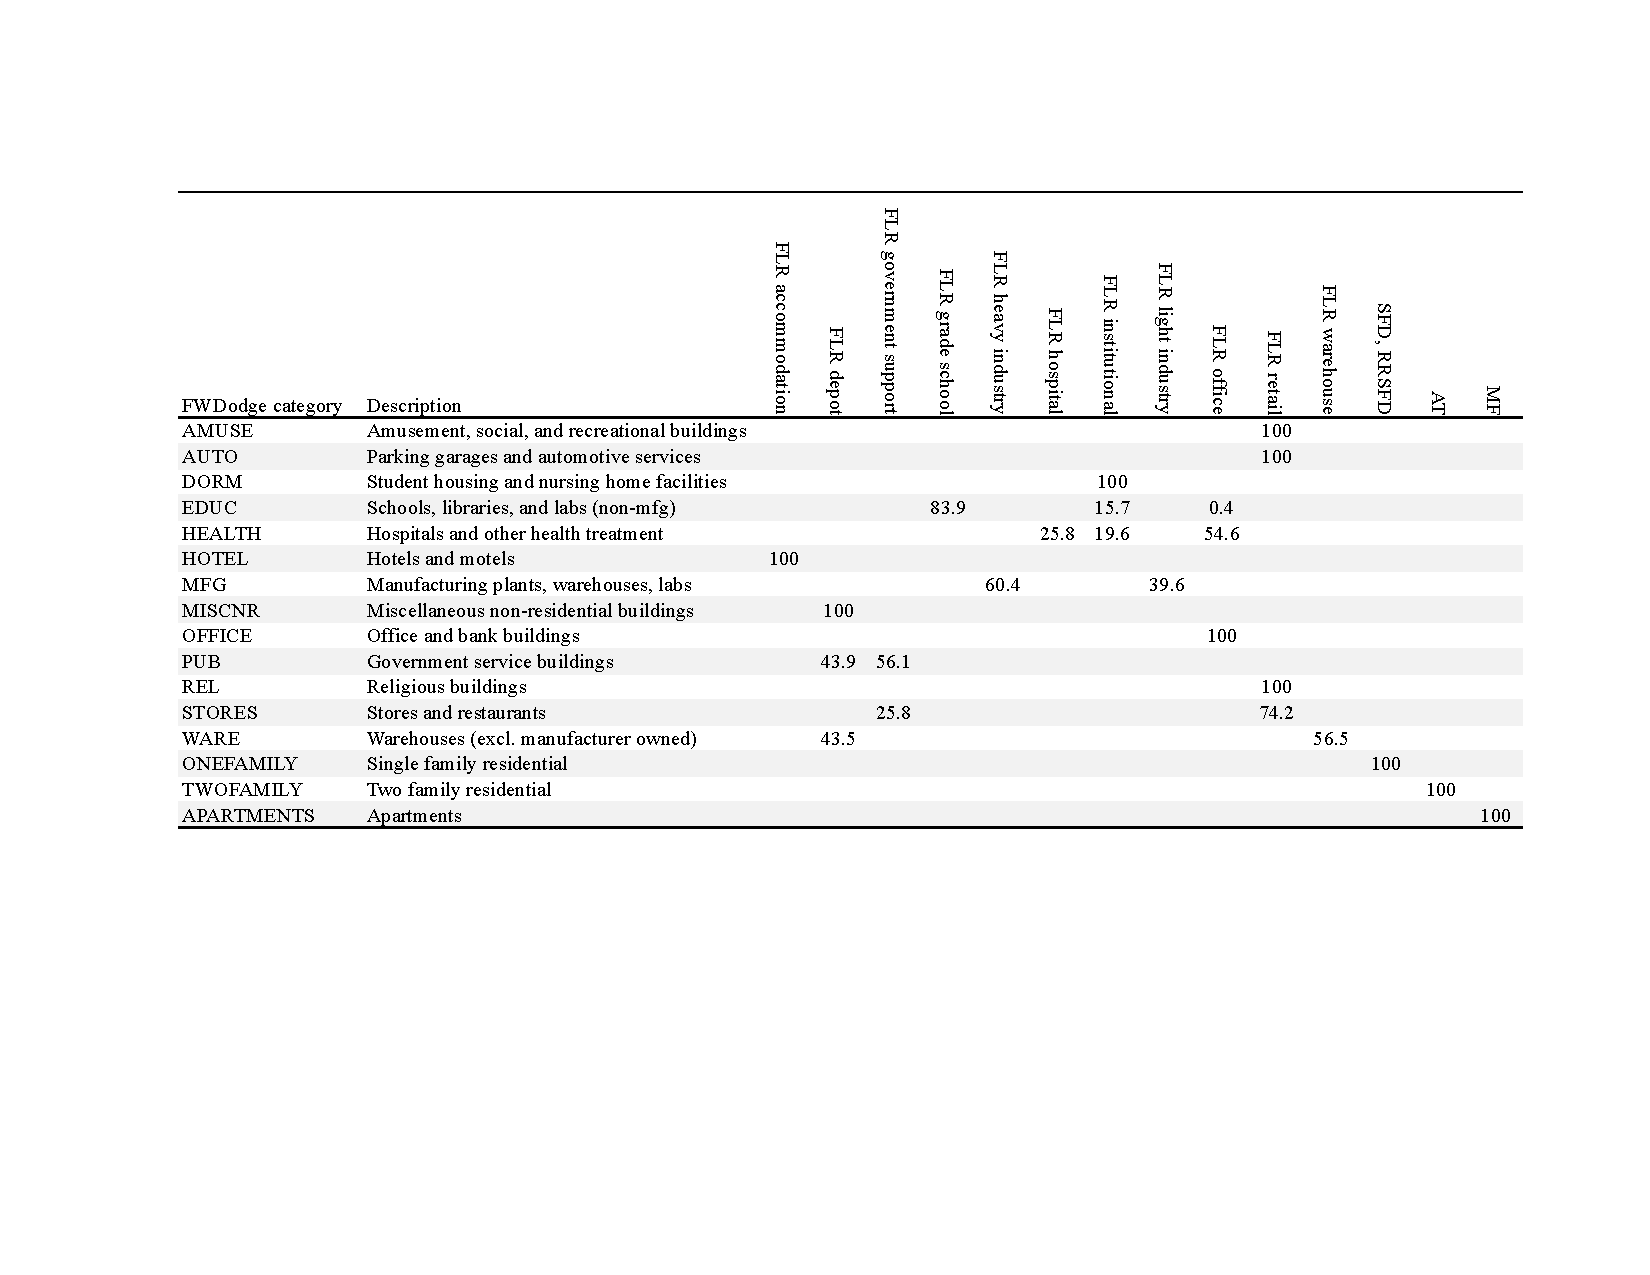
\includegraphics[scale=0.95, trim=28mm 70mm 20mm 32mm, clip]{ald/building-space-mapping} % trim=l b r t
\end{sidewaystable}

\begin{figure}
\centering
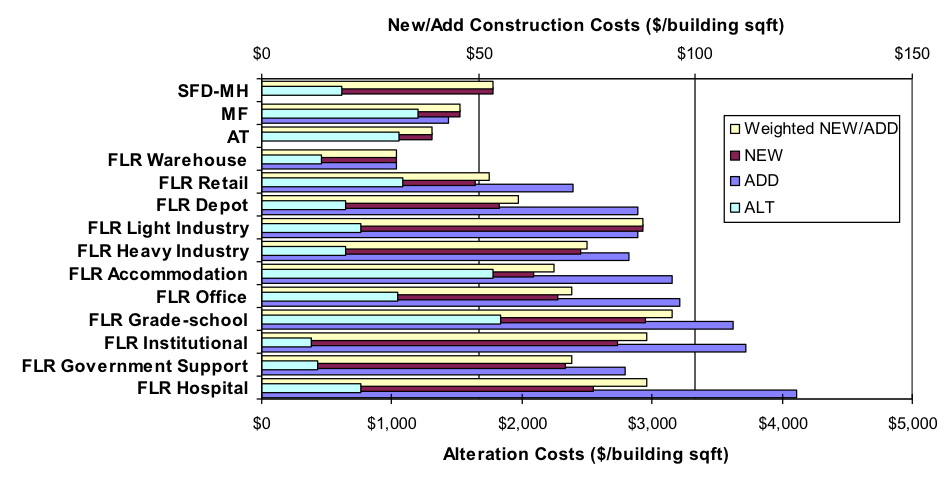
\includegraphics[scale=0.45]{ald/average-construction-costs}
\caption{Statewide average construction costs}\label{fig:average-construction-costs}
\end{figure}

\subsection{Modelwide Floorspace Value Decrease Factors (Df)}\label{sec:ald-floorspace-decrease-factors}   % 5.5.2
Residential and non-residential floorspace decrease factors were computed by comparing the average floorspace construction values produced by the ED module (prior to current NED model) for the period between 1990 and 2000, with the value of the change in floorspace computed from the FW Dodge data for the same period. The latter was calculated by multiplying the change in square footage computed from the FW Dodge data for each floorspace category by the unit construction cost rates estimated in Section \ref{sec:ald-unit-cost-rates}. The resulting decrease factors estimated in this way were 0.12 for residential and 0.39 for nonresidential.

Comparison of forecast and independent data in this way is rational but not a very rigorous exercise, but required in the face of limited data. In 2010, after early use of the model indicated that non-residential floorspace availability limitations from ALD were contributing to AA module convergence issues over time, these coefficients were revisited. As such, during calibration it was felt that a reduction in the non-residential factor was a reasonable action. Under this effort, the residential factor of 0.12 was applied to both residential and non-residential space types, significantly reducing the non-residential demolition. Some further sensitivity testing of this value may be of useful.

The values currently used by ALD are 0.12 for residential and nonresidential value. These Df values are stored in ALDResCoefficients.csv and ALDNresCoefficients.csv, respectively, which are found in the ``inputs/parameters'' folder.


\subsection{Land Capacity Calculation Parameters}\label{sec:ald-capacity-parameters}  % 5.5.3
The values of the Land Capacity Calculation parameters discussed in Section \ref{sec:ald-step2}, after S2 validation, including the dispersion parameter ($\lambda_p$), size term and coefficient ($size_f$, $stc$), are shown in Table \ref{tab:land-capacity-parameters}. In validation, significant adjustments were also made to the exogenous inputs of the compatibility matrix and FAR data. The $sizef$ term represents modelwide land area devoted to each floorspace type, developed from a modelwide GIS 30m grid coverage of built form (Development Type and Quantity of space) synthesized for the SWIM2 LD module.
% [10]

\begin{table}[!t]  % 5-3
\centering
\caption{ALD land capacity function parameters}\label{tab:land-capacity-parameters}
\begin{tabular}{llr}
\hline
Parameter & Description & Value \\
\hline
$\lambda_p$ & Dispersion parameter & 0.075 \\
stc & Size parameter & 1 \\
$size_f$ & FLR MH & 135,895,174 \\
 & FLR MF & 253,651,065 \\
 & FLR AT & 111,905,458 \\
 & FLR SFD & 1,385,141,602 \\
 & FLR RRMH & 82,164,425 \\
 & FLR RRSFD & 453,931,807 \\
 & FLR Accommodation & 29,262,691 \\
 & FLR Depot & 53,476,910 \\
 & FLR Government support & 111,166,124 \\
 & FLR Grade-school (K12) & 165,712,129 \\
 & FLR Heavy industry & 21,409,696 \\
 & FLR Hospital & 35,095,111 \\
 & FLR Institutional & 80,154,397 \\
 & FLR Light industry & 184,975,915 \\
 & FLR Office & 317,827,388 \\
 & FLR Retail & 193,736,194 \\
 & FLR Warehouse & 135,895,174 \\
\hline
\end{tabular}
\end{table}


\subsection{Model Parameters for Allocating Modelwide Construction Dollars into Regional Dollar Value Increases and Decreases}\label{sec:ald-increase-decrease}   % 5.5.4
ALD parameters were calibrated for functions that split ED (Now NED) module model wide residential and nonresidential construction dollars into region-level dollar increases and decreases (see \S\ref{sec:ald-step1}). For the purposes of S2 calibration, data from the Bureau of Economic Analysis' Regional Economic Information System (REIS) was used to measure activity. Employment was used as the measure of activity related to non-residential floorspace. Population was used as the measure of activity related to residential floorspace.

In S3 calibration, AA activity data will be used. The parameters for the increase and decrease functions were calibrated simultaneously using evolutionary algorithms. A population of 2000 parameter combinations was generated at random from a set of defined parameter bounds and run through 42 evolutionary steps to find the best fitting parameter combination. In each evolutionary step, increases and decreases were calculated and summed to calculate a net change by region.

The RMSE error between the calculated regional net changes and the regional changes calculated from the FW Dodge data was used as a fitness measure to identify the best fitting parameter combinations. The best fitting combinations were then modified through ``crossovers'' or ``mutations'' to produce a new population of 2000 parameter combinations used in the next step. Figure \ref{fig:residential-parameter-convergence} shows an example of convergence of residential floorspace increase function parameters. Figure \ref{fig:fwdodge-target-convergence} shows a corresponding example of the convergence of model net results to the FW Dodge target values for four regions. The resulting alternative specific constants are included in Tables \ref{tab:nonresidential-construction-asc} and \ref{tab:residential-construction-asc} for nonresidential and residential floorspace types, respectively (note that the Depot field was dropped for implementation with AA). The values for the four Cobb-Douglas production parameters are shown in Table \ref{tab:coff-douglas-parameters}.

\begin{sidewaystable}
\centering
\caption{Alternative-specific constants to allocate non-residential regional construction}\label{tab:nonresidential-construction-asc}
\small
\begin{tabular}{lrrrrrrrrrrr}
\hline
       & Accom- &       & Gov't   & Grade  & Heavy    &          & Institu- & Light    &        &        & Ware- \\
Region & modation   & Depot & Support & school & industry & Hospital & tional   & industry & Office & Retail & house \\
\hline
\multicolumn{12}{c}{Increase (inputs/parameters/ALDAsc1.RgFn.csv)} \\
\hline
Astoria\_LincolnCity & 0.944702 & 0.235614 & -0.259910 & 0.207471 & -2.907440 & 0.432939 & -0.081280 & -1.401530 & -0.741630 & 0 & -0.80103 \\
\gray BakerCity\_JohnDay & 0.586089 & 1.625532 & 1.801039 & 1.407736 & 1.504913 & 1.514356 & 1.926353 & 0.767333 & 0.735611 & 0 & -0.21093 \\
Bend & -0.884470 & 0.423798 & -0.349120 & 0.394332 & -1.880110 & -0.661790 & -1.066460 & -2.156670 & -0.397320 & 0 & -2.45611 \\
\gray Eugene & 0.699288 & 0.948542 & -1.294870 & -0.517360 & -1.251130 & 0.616967 & -0.096580 & -0.903660 & 0.458251 & 0 & -1.07190 \\
Eureka\_Brookings & 0.183214 & 0.072535 & 0.413877 & -0.792110 & -1.361930 & 0.714911 & 0.367652 & -0.367840 & -1.051680 & 0 & -0.81388 \\
\gray KlamathFalls\_Burns & 2.007493 & 0.904102 & 0.418304 & -0.045670 & -2.060080 & 1.614082 & 0.350857 & 0.120022 & 0.476692 & 0 & -0.56112 \\
Lewistown & 1.140614 & 1.039634 & 0.021470 & 1.676284 & -0.949050 & 1.471895 & 0.627516 & -1.017900 & 0.443534 & 0 & -0.66874 \\
\gray Longview\_Centralia & 0.145686 & 0.783508 & -0.723700 & -0.682170 & -0.822890 & 0.524477 & -1.092800 & -1.209510 & -0.484420 & 0 & -0.81174 \\
Medford\_GrantsPass & -0.008700 & -0.121280 & -0.623880 & -0.288720 & -0.944310 & 0.050372 & -0.001280 & -0.684090 & -0.257270 & 0 & -1.07863 \\
\gray Ontario\_Boise & 0.277807 & 0.494493 & -0.394450 & 0.146705 & -0.856080 & -0.350780 & -0.223810 & -0.876460 & 0.371850 & 0 & -1.44383 \\
Portland\_Vancouver & 0.086280 & 1.083125 & -1.308010 & -0.080430 & -0.828400 & -1.003140 & -0.586460 & -0.067400 & -0.086880 & 0 & -1.14624 \\
\gray Salem & 0.687471 & 1.323692 & -0.206050 & 0.244056 & -2.442220 & 0.217611 & -0.171280 & -2.377680 & -0.019380 & 0 & -0.99943 \\
TheDalles & -1.261090 & -0.51397 & -0.821790 & 0.332557 & -2.600690 & 1.032134 & 0.389188 & -3.854760 & -0.361730 & 0 & -1.24701 \\
\gray Yakima\_Pendleton & 0.483384 & 1.80530 & -0.398530 & 1.823500 & 0.272279 & 0.328345 & 1.068840 & 0.151031 & 0.850889 & 0 & -0.50899 \\
Yreka\_Redding & -0.096830 & -0.16398 & 0.622854 & 0.014584 & -1.37370 & 0.844414 & 1.112208 & -2.005020 & 0.295520 & 0 & -0.95297 \\
\hline
\multicolumn{12}{c}{Decrease (inputs/parameters/ALDAsc2.RgFn.csv)} \\
\hline
\gray Astoria\_LincolnCity & 2.763757 & -0.854408 & 0.550963 & -0.588357 & 2.171298 & -0.293591 & -0.729383 & 1.650154 & 0.827490 & 0 & -0.810913 \\
BakerCity\_JohnDay & -0.891268 & 1.010798 & 2.249196 & 2.157934 & 1.961006 & -1.042788 & 1.813892 & -0.465579 & 0.459310 & 0 & -1.913085 \\
\gray Bend & -0.460973 & 2.013159 & 2.660423 & 3.029211 & 2.405165 & 0.022755 & 0.053865 & 2.891694 & 1.527273 & 0 & -1.002809 \\
Eugene & -0.040206 & 2.570598 & -3.038275 & 0.235208 & 1.123078 & 2.402918 & -0.522408 & -0.052002 & 0.954050 & 0 & 0.541387 \\
\gray Eureka\_Brookings & 1.101352 & 0.885427 & 1.274713 & 0.741928 & 3.300662 & 0.772333 & 1.338762 & 3.018789 & 1.374824 & 0 & -0.496001 \\
KlamathFalls\_Burns & 0.781087 & 0.145467 & -0.085089 & -0.134997 & -0.002645 & 0.367056 & -1.208864 & 0.117831 & -0.319939 & 0 & -2.070174 \\
\gray Lewistown & 1.274683 & 1.499027 & 0.648288 & 2.126220 & 1.051077 & 0.914092 & -0.326581 & -0.350138 & 0.496095 & 0 & -0.821363 \\
Longview\_Centralia & 0.393504 & 1.158247 & -0.788388 & 0.676693 & 1.232855 & 1.975634 & -2.210476 & 1.070667 & 0.726616 & 0 & -0.175315 \\
\gray Medford\_GrantsPass & -0.147762 & 0.387470 & -0.288341 & 0.058904 & 2.180457 & -1.012891 & 1.545078 & 2.765504 & -0.164663 & 0 & 0.073767 \\
Ontario\_Boise & 0.584221 & 1.205850 & -0.251980 & -1.078799 & 2.275093 & 0.240065 & -0.487524 & 1.986376 & -0.335838 & 0 & 0.519281 \\
\gray Portland\_Vancouver & 1.363668 & 3.348070 & 0.122153 & 0.825876 & -0.962027 & -2.057667 & 0.743412 & 0.649737 & 1.054240 & 0 & 0.410136 \\
Salem & -0.082270 & 0.369023 & 1.562376 & 1.748439 & 0.128730 & 0.642501 & -0.449637 & -0.071461 & 0.692468 & 0 & -1.009280 \\
\gray TheDalles & -2.619944 & -2.514178 & -3.461466 & -3.148120 & -1.094045 & -3.291059 & -2.679318 & 3.974732 & -1.877617 & 0 & -2.478947 \\
Yakima\_Pendleton & -1.287373 & -1.349710 & -1.908386 & 2.254272 & 2.243717 & -1.789344 & 2.383304 & 2.847587 & 0.956473 & 0 & -1.576993 \\
\gray Yreka\_Redding & 1.226759 & -0.823016 & 1.439139 & 1.297564 & 0.675903 & 2.622162 & -0.211855 & 0.785988 & 1.974681 & 0 & 0.561401 \\
\hline
\end{tabular}
\end{sidewaystable}  % 5-4
\begin{table}
\centering
\caption{Alternative-specific constants to allocate residential regional construction}\label{tab:residential-construction-asc}
\begin{tabular}{lrrrrrr}
\hline
Region & MH & MF & AT & SFD & RRMH & RRSFD \\
\hline
\multicolumn{7}{c}{Increase (inputs/parameters/ALDAsc1.RgFr.csv)} \\
\hline
Astoria\_LincolnCity & 0.599185 & -0.09141 & 0.128806 & 0 & 0.32678 & 0.208994 \\
\gray BakerCity\_JohnDay & -0.28148 & -0.27616 & -0.43235 & 0 & -0.27724 & -0.34203 \\
Bend & 0.516327 & -0.53798 & -0.08595 & 0 & 0.838234 & 0.705884 \\
\gray Eugene & 0.117779 & 0.386703 & 0.844898 & 0 & -0.20865 & 0.002161 \\
Eureka\_Brookings & -0.06574 & -3.14471 & -3.61438 & 0 & -0.14144 & 0.498804 \\
\gray KlamathFalls\_Burns & 0.260061 & -0.22102 & 0.365183 & 0 & 0.421043 & 0.180597 \\
Lewistown & -0.21071 & -0.0555 & -0.01667 & 0 & -0.46303 & 0.319172 \\
\gray Longview\_Centralia & 0.271002 & -0.43668 & -0.34781 & 0 & 0.264514 & 1.194059 \\
Medford\_GrantsPass & 0.638162 & 0.274419 & 0.659648 & 0 & 0.395957 & 0.306998 \\
\gray Ontario\_Boise & -0.15147 & -0.94255 & -0.60234 & 0 & -1.02368 & 0.039501 \\
Portland\_Vancouver & 0.056183 & 0.073551 & 0.083727 & 0 & -0.73026 & 0.168127 \\
\gray Salem & 0.330187 & 0.338436 & 0.381144 & 0 & -0.20455 & 0.058002 \\
TheDalles & 0.448967 & -0.12737 & -0.0613 & 0 & 0.656301 & 1.422753 \\
\gray Yakima\_Pendleton & -0.36111 & -0.34582 & -0.45934 & 0 & -0.86607 & 0.432256 \\
Yreka\_Redding & -0.09976 & -0.24731 & -1.02394 & 0 & 0.283882 & 0.943806 \\
\hline
\multicolumn{7}{c}{Decrease (inputs/parameters/ALDAsc2.RgFr.csv)} \\
\hline
\gray Astoria\_LincolnCity & -1.84316 & -2.11438 & -3.64243 & 0 & -0.34124 & 0.111757 \\
BakerCity\_JohnDay & -2.84376 & -2.54353 & -3.50431 & 0 & -3.5544 & -2.39588 \\
\gray Bend & -2.31471 & -2.72093 & -2.86904 & 0 & -0.16878 & 1.979141 \\
Eugene & -2.09872 & -2.08561 & -1.92973 & 0 & -3.51411 & -0.59056 \\
\gray Eureka\_Brookings & -0.72992 & 0.928168 & 1.34931 & 0 & -3.59163 & 2.059602 \\
KlamathFalls\_Burns & -0.7994 & -2.39492 & -1.91467 & 0 & -2.25349 & -0.95675 \\
\gray Lewistown & -2.24869 & 0.179987 & -3.12329 & 0 & -1.48853 & -1.38146 \\
Longview\_Centralia & -2.3721 & -2.68488 & -1.009 & 0 & -1.44889 & 3.038585 \\
\gray Medford\_GrantsPass & -1.02841 & 0.355648 & -2.98606 & 0 & 0.255433 & 0.244647 \\
Ontario\_Boise & -0.05595 & -1.92675 & -0.26284 & 0 & -0.67294 & 3.677403 \\
\gray Portland\_Vancouver & -2.94502 & -3.14238 & -1.00111 & 0 & -3.17513 & 3.70538 \\
Salem & -3.3574 & -0.15295 & -0.62065 & 0 & -2.34857 & -2.15255 \\
\gray TheDalles & -1.2888 & -1.5701 & -2.09202 & 0 & -1.66081 & 1.975529 \\
Yakima\_Pendleton & -1.36691 & -0.85531 & -0.24308 & 0 & -1.40415 & 3.92212 \\
\gray Yreka\_Redding & -0.20314 & -1.31216 & -2.26709 & 0 & -2.96348 & 3.482707 \\
\hline
\end{tabular}
\end{table}   % 5-5

\begin{figure}[!t]
\centering
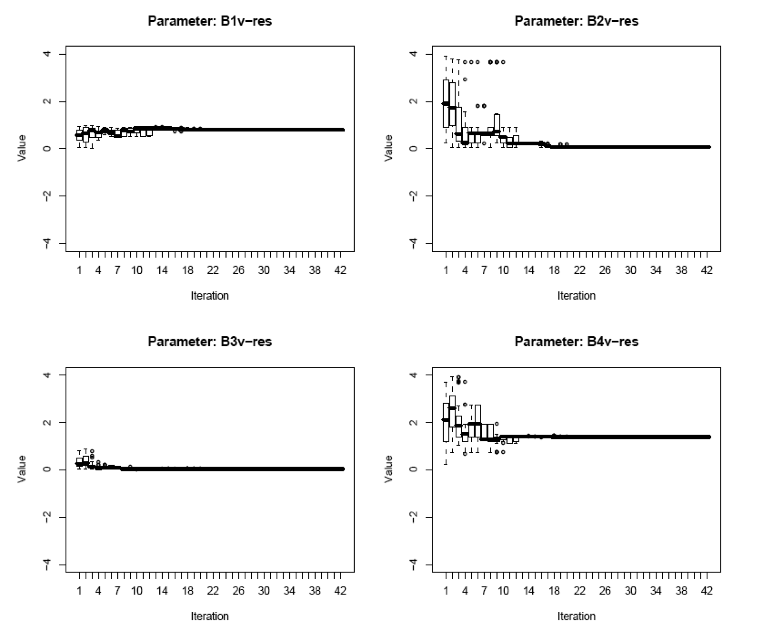
\includegraphics[width=6in]{ald/residential-parameter-convergence}
\caption{Convergence of residential parameter values}\label{fig:residential-parameter-convergence}
\end{figure}

\begin{figure}[!t]
\centering
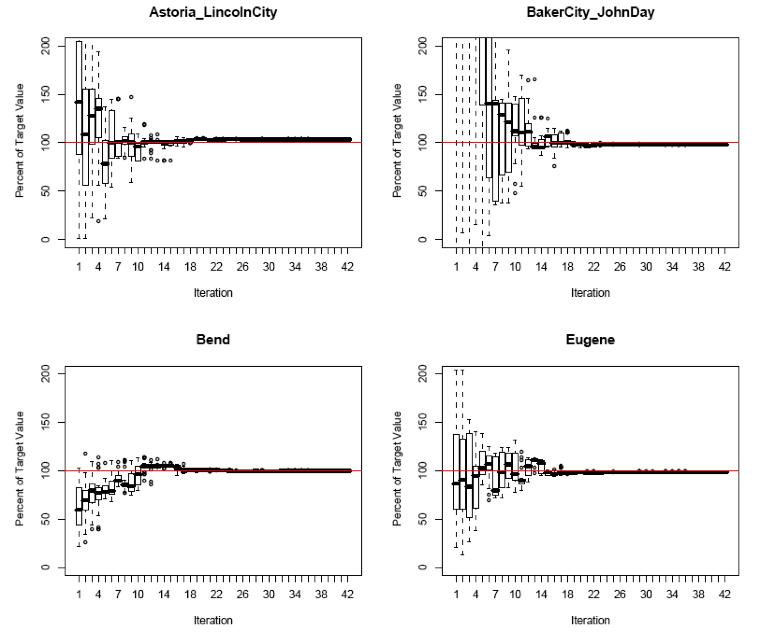
\includegraphics[width=6in]{ald/fwdodge-target-convergence}
\caption{Convergence of model results to FW Dodge target values}\label{fig:fwdodge-target-convergence}
\end{figure}

During 2015 S3 review of the modelwide construction dollars over time it was learned that ALD was far too sensitive to changes in regional activity from ALD. To counteract this, judgment from the team was applied. The parameters estimated above had an exponential term of approximated 2 (2.36 for non-residential and 1.96 for residential) on the activity change side of Equation \ref{eq:5.02}. After through review and testing it was determined that a more appropriate value for this term was a required a reduction by approximately one order of magnitude. Therefore, both residential and non-residential $\beta_{4v}$ parameters were set to 0.2 (this is reflected in Table \ref{tab:coff-douglas-parameters}).

\begin{table}   % 5.6
\centering
\caption{ALD Cobb-Douglas parameters}\label{tab:coff-douglas-parameters}
\begin{tabular}{clrr}
\hline
Parameter & Description & Nonresidential & Residential \\
\hline
$\beta_{1v}$ & Activity proportion additive term & 0.278924 & 0.707674 \\
$\beta_{2v}$ & Activity change proportion additive term & 1.968482 & 1.608066 \\
$\beta_{3v}$ & Activity proportion power & 0.399309 & 0.167152 \\
$\beta_{4v}$ & Activity change proportion power & 0.2 & 0.2 \\
\hline
\end{tabular}
\end{table}

Further, after this review it was determined that the decreasing set of parameters were likely incorrect as well. However, since there is far less data and information on how floorspace is converted (reduced and modified), the team opted to use the identical set of parameters used for the allocation of increase in dollars as in decrease. This was deemed acceptable, since this stage of the model is only working on total construction dollars by the 15 ALD regions; producing 30 highly aggregate values (15 for residential and 15 for non-residential) across the entire model area. The decision being that the level of precision at this level is not as great of a concern as it would be at more disaggregate decision points in the model.
  

\subsection{Model Parameters for Allocating Regional Dollar Increases and Decreases into Floorspace Types}\label{sec:ald-allocate-inc-dec}   % 5.5.5
The search space to find the best fit of parameters for the allocation of regional dollar development changes into floorspace type (see \S\ref{sec:ald-step2}) was very large, because of the significant number of alternative specific constants. Both the increase and decrease functions require an alternative specific constant for every combination of region and floorspace type. In order to get convergence and to ``maximize'' the share of ``behavior'' explained by the model parameters vs. the alternative specific constants, the process of calibrating this step was split into two parts. In the first part, the range of possible values for the alternative specific constants was constrained. 36 evolutionary steps were run to get the best fit results for the parameters. The best results from the first part were then processes through a second round of 25 evolutionary steps where the alternative specific constants were varied through a wider range of values. Figure \ref{fig:bend-floorspace-convergence} shows an example of the convergence of the proportional distribution of model net floorspace change to the FW Dodge target proportions for the Bend region. Tables \ref{tab:floorspace-allocation-parameters} and \ref{tab:floorspace-asc} show estimated parameter values.

\begin{figure}
\centering
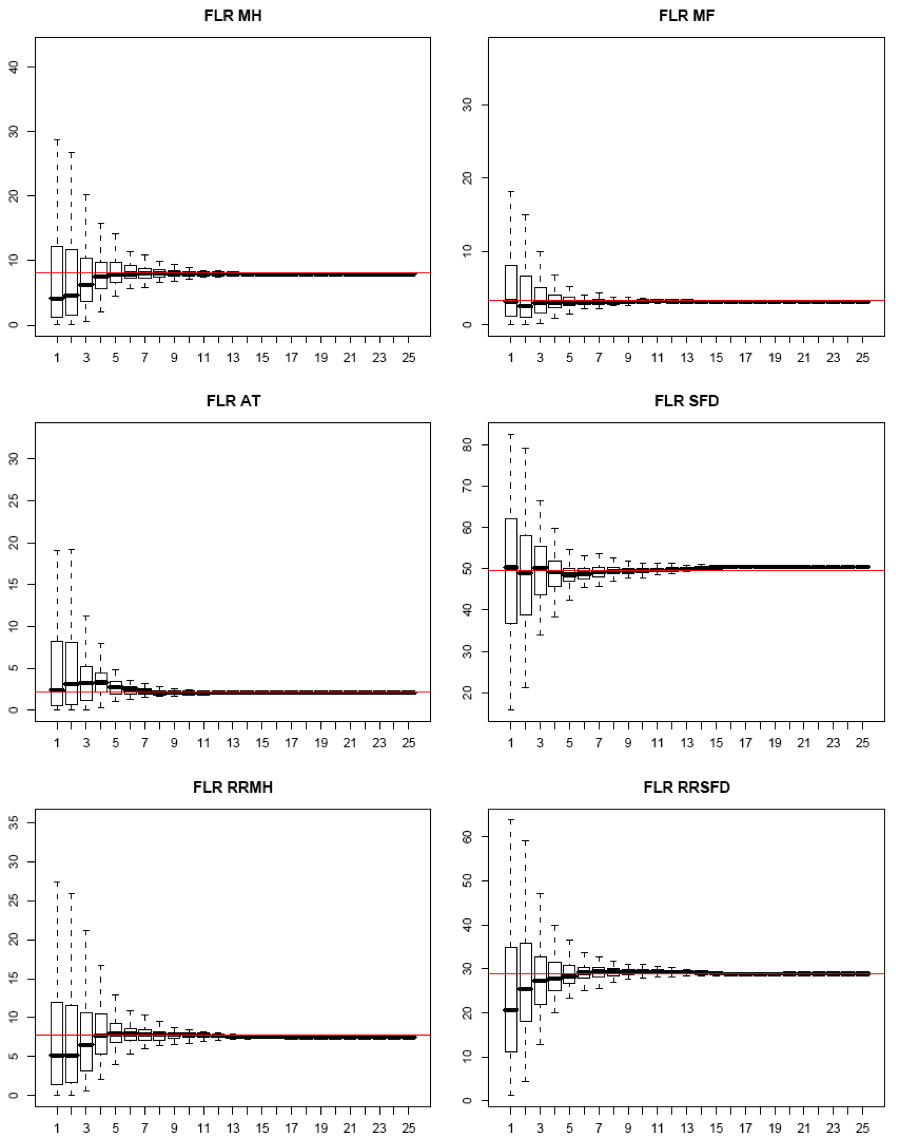
\includegraphics[width=6in]{ald/bend-floorspace-convergence}
\caption{Convergence of Bend Region model floorspace results to FWDodge target values}
\label{fig:bend-floorspace-convergence}
\end{figure}

\begin{table}[!t]    % 5-7
\centering
\caption{ALD parameters for allocation to floorspace types}\label{tab:floorspace-allocation-parameters}
\begin{tabular}{lclrr}
\hline
Category & Parameter & Description & Increase & Decrease \\
\hline
Nonresidential & $\lambda_{q1}, \lambda_{q2}$ & Dispersion parameter & 0.577946 & 0.309236 \\
 & $\beta_{q1}, \beta_{q3}$ & Sensitivity to vacancy rate: \\         
 & & FLR Accommodation & -0.448740 & -1.390874 \\
 & & FLR Depot (removed in AA) & -0.685066 & -1.770418 \\
 & & FLR Government Support & -0.717076 & -1.998696 \\
 & & FLR Grade-school & -1.081031 & -1.048652 \\
 & & FLR Heavy Industry & -2.992417 & -0.667520 \\
 & & FLR Hospital & -0.463261 & -1.030110 \\
 & & FLR Institutional & -0.387125 & -1.058415 \\
 & & FLR Light Industry & -2.197701 & -1.830717 \\
 & & FLR Office & -2.128987 & -2.648114 \\
 & & FLR Retail & -0.509895 & -1.394915 \\
 & & FLR Warehouse & -1.922216 & -1.823896 \\
 & $\beta_{q2}, \beta_{q4}$ & Sensitivity to prior year proportion & 0.874475 & 0.932353 \\
\hline
Residential & $\lambda_{q1}, \lambda_{q2}$ & Dispersion parameter & 1.016924 & 1.48071 \\
 & $\beta_{q1}, \beta_{q3}$ & Sensitivity to Vacancy rate: \\
 & & FLR MH & -2.68199 & 2.09219 \\
 & & FLR MF & -3.84517 & 2.71393 \\
 & & FLR AT & -3.60789 & 2.21573 \\
 & & FLR SFD & -2.24556 & 1.47095 \\
 & & FLR RRMH & -1.49781 & 1.55033 \\
 & & FLR RRSFD & -1.97620 & 3.11092 \\
 & $\beta_{q2}, \beta_{q4}$ & Sensitivity to prior year proportion & 0.993564 & 0.881172 \\
\hline
\end{tabular}
\end{table}

As with the previous section, S3 review conducted in 2015 showed that ALD region construction dollar increase and decreases did not match reasonable expectations. The issue was that any given ALD region could gain vastly more or substantially less construction activity over time than their size suggested. The calibrated parameters appeared to work for the calibrated base year, but then would become unstable over the course of the model. To adjust for this, model runs were made over the 30 year model horizon. Relative size targets for each ALD region were established over a history of census and employment information. The relative size by population over time of each ALD region was used as a guide or target residential construction dollars, and employment over time was used for non-residential construction dollars. An iterative process was then conducted where full SWIM model runs were done with successively iterating the parameter values found in Table \ref{tab:floorspace-asc}. This was conducted for several months until a final set of ALD region specific constants were established that held the regional construction dollar allocation in relative balance overtime. The model is still reactive to changes from scenarios, but is now better balanced to match high level expectations under the reference condition. The resulting parameters are shown in Table \ref{tab:floorspace-asc}.
 
\begin{table}
\centering
\caption{ALD allocation to floorspace types alternative specific constants}\label{tab:floorspace-asc}
\begin{tabular}{lcccc}
\hline
 & \multicolumn{2}{c}{Decrease} & \multicolumn{2}{c}{Increase} \\
Region & Residential & Non-residential & Residential & Non-residential \\
\hline
Astoria\_LincolnCity & 0.37 & 0.46 & 0.37 & 0.46 \\
\gray BakerCity\_JohnDay & 0.19 & 0.20 & 0.19 & 0.20 \\
Bend & 0.55 & 0.63 & 0.55 & 0.63 \\
\gray Eugene & 1.19 & 1.16 & 1.19 & 1.16 \\
Eureka\_Brookings & 0.55 & 0.60 & 0.55 & 0.60 \\
\gray KlamathFalls\_Burns & 0.21 & 0.25 & 0.21 & 0.25 \\
Lewistown & 0.48 & 0.67 & 0.48 & 0.67 \\
\gray Longview\_Centralia & 0.51 & 0.59 & 0.51 & 0.59 \\
Medford\_GrantsPass & 0.74 & 0.81 & 0.74 & 0.81 \\
\gray Ontario\_Boise & 1.58 & 1.92 & 1.58 & 1.92 \\
Portland\_Vancouver & 2.76 & 2.09 & 2.76 & 2.09 \\
\gray Salem & 1.49 & 1.43 & 1.49 & 1.43 \\
TheDalles & 0.21 & 0.28 & 0.21 & 0.28 \\
\gray Yakima\_Pendleton & 1.52 & 1.86 & 1.52 & 1.86 \\
Yreka\_Redding & 0.80 & 0.88 & 0.80 & 0.88 \\
\hline
\end{tabular}
\end{table}


\subsection{Model Parameters for Allocating Regional Floorspace Decreases and Increases to Alpha zones}\label{sec:ald-inc-dec-alpha}   % 5.5.6
The parameters influencing the zonal-level decrease and increase of floorspace by type, described in Sections \ref{sec:ald-step3} and \ref{sec:ald-step4}, were calibrated against the FW Dodge county change in net floorspace stock. In other words, upon completion of the net change in floorspace by alpha zone and type, the results are summed to the county level and compared with the FW Dodge data. As with the previous two steps, an evolutionary algorithm was used to calibrate the parameters. Unlike the other steps, however, there are no alternative specific constants, so the number of parameters to calibrate is smaller (but not small). This allowed there to be fewer evolutionary rounds. This was also necessary because these models have many more computations and require significantly more computing time per round. Only twelve evolutionary rounds were used. The results are not nearly as good as in the previous two steps. This is to be expected in part because this step creates a substantial disaggregation of the results. It is expected that this will improve in the S3 calibration. Resulting parameter values are shown in Table \ref{tab:zonal-floorspace-alloc}.

\begin{table}  % 5.9
\centering
\caption{ALD zonal floorspace allocation parameters}\label{tab:zonal-floorspace-alloc}
\begin{tabular}{lclrr}
\hline
Category & \multicolumn{2}{l}{Parameter} & Non-residential & Residential \\
\hline
Decrease & $\beta_{3f}$ & Prior year proportion dispersion & 1.963554 & 1.248889 \\
 & $\beta_{4f}$ & Price dispersion & -0.269004 & -0.271316 \\
\hline
Increase & $\beta_{5f}$ & Prior year proportion dispersion & 1.729279 & 1.160029 \\
 & $\beta_{6f}$ & Price dispersion & 0.347738 & 0.284712 \\
 & $\beta_{7f}$ & Prior year saturation factor & 0.248170 & 0.052244 \\
 & $\beta_{8f}$ & Prior year saturation dispersion & 5.817253 & 6.642847 \\
 & $\beta_{9f}$ & Prior year proportion additive term & 0.002111 & 0.000673 \\
\hline
\end{tabular}
\end{table}

\section{Inputs and Outputs}
ALD inputs and outputs are listed in Tables \ref{tab:ald-inputs} and \ref{tab:ald-outputs}. ALD requires current year construction activity values from NED and previous year activity (two-year) occupancy and price data from AA. Vacancy rates are calculated as the ratio of previous year AA occupied floorspace to previous year ALD total floorspace quantity. Zoning-based land capacities by alpha zone are exogenously developed for each year using GIS. Values for $ConsCostf$ are drawn from FWDodge construction starts data between 1990 and 2001 and were then inflated to 2009 dollars. Additional ALD definition files are also required to run the model. Detailed descriptions of several ALD input data are discussed in the remainder of this section.

ALD produces a current year floorspace inventory for AA (and for use in ALD in the next year). The agriculture and logging lands are adjusted in the AA file, as discussed in \S\ref{sec:ald-completing-inventory}. In addition to the outputs used by other modules, ALD prints a series of diagnostic files listed also in Table \ref{tab:ald-outputs}.

\begin{table}[!t]    % Table 5-10
\centering
\caption{ALD inputs}\label{tab:ald-inputs}
\begin{tabular}{p{4.8in}l}
\hline
Data element & Source \\
\hline
Modelwide construction activity \$ for residential (\$res) and nonresidential (\$nres) categories [construction\_forecast.csv] & NED \\
\gray Beta Zone activity demand (HHs and industry \$ by type) [ExchangeResults.csv] & Current year AA \\
Modelwide occupied floorspace (sqft) by floorspace category [ExchangeResults.csv] & Current year AA \\
\gray Unit prices for residential and nonresidential space in alpha zones [ExchangeResults.csv] & Current year AA \\
Building square footage by alpha zone (row) and floorspace type (col) [FloorspaceInventory.csv] & Previous year ALD \\
\gray Alpha-beta zone conversion [alpha2beta.csv] & SI \\
Modelwide space construction costs per square foot by floorspace type [ConstructionCosts.csv] & Exogenous \\
\gray Matrix of land square feet by alpha zone and zoning category (zonal input) [LandSQFTxzoning.csv] & SI \\
Matrix of floor to area ratios by floorspace type (rows) and zoning category (cols) [far.csv] & Exogenous \\
\gray Matrix of compatibility values (NP-0 to VH-1=best) by floorspace type (row) and zoning category (col) [zoning\_compatibility.csv] & Exogenous \\
Definition files [floorspace\_definitions][zoning\_definitions] & Exogenous \\
\gray Land Capacity Size term values [LandSQFTxFLR.csv] & Exogenous \\
\hline
\end{tabular}
\end{table}

% Table 5 11 ALD Outputs
\begin{table}[!t]    % Table 5-11
\centering
\caption{ALD outputs}\label{tab:ald-outputs}
\begin{tabular}{p{4.8in}l}
\hline
Description & Users \\
\hline
Building square footage (landsqft for agriculture and logging) by alpha zone (row) and floorspace type (col) [FloorspaceInventory.csv] & PT, next year ALD \\ 
\gray AA-format building square footage (landsqft for agriculture and logging) by alpha zone (row) and floorspace type (col) [FloorspaceI.csv] & AA \\
Floorspace type split within each zoning category [FloorspaceProportionsByZoning.csv] & Diagnostics \\
\gray Building space increase for each floorspace type in each alpha zone [Increments.csv][Increments\_Matrix.csv] & AA, diagnostics \\
Land sqft of each floorspace type in each alpha zone [LandAllocations.csv] & Diagnostics \\
\gray Building sqft zoning capacity of each floorspace type in each alpha zone [ResidentialCapacity.csv] [NonresidentialCapacity.csv] & Diagnostics \\
Ratio of floorspace after decrease (but before increase) to total floorspace capacity [CapacityUtilization.csv] & Diagnostics \\
\gray Building Msqft decrease of each floorspace type in each alpha zone [ResidentialDecrease.csv] [NonresidentialDecrease.csv] & Diagnostics \\
Decrease utility for each floorspace type in each alpha zone [ResidentialDecreaseUtilities.csv] [NonresidentialDecreaseUtilities.csv] & Diagnostics \\
\gray Building Msqft increase of each floorspace type in each alpha zone [ResidentialIncrease.csv] [NonresidentialIncrease.csv] & Diagnostics \\
Increase utility for each floorspace type in each alpha zone [ResIncreaseUtilities.csv] [NonresIncreaseUtilities.csv] & Diagnostics \\
\gray Building Msqft after decrease (before increase) of each floorspace type in each alpha zone  [ResQuantititesAfterDecrease.csv] [NonresQuantititesAfterDecrease.csv] & Diagnostics \\
Log file for ALD run [ald.Rout] & Diagnostics \\
\gray R workspace from most recent run [.RData] & Diagnostics \\
Matrix of alpha zone/floorspace types where capacity less than floorspace quantity (after decrease) [ResLowCapacity.csv] [NonresLowCapacity.csv] & Diagnostics \\
\hline
\end{tabular}
\end{table}

\subsection{Base year Floorspace Estimates}\label{sec:ald-baseyear-floorspace}  % 5.6.1
Floorspace is difficult to gather statewide at any sub-county level. To be consistent with the space needed for AA activities (see \S\ref{sec:aa-pc-allocation} on page \pageref{sec:aa-pc-allocation}), a modelwide floorspace inventory (by alpha zone) was synthesized for the base year to cover four categories:
\begin{itemize}
\item Residential building floorspace (building sqft).
\item Non-residential housing floorspace (building sqft).
\item Productive agricultural lands (land sqft).
\item Productive logging timberlands (land sqft). 
\end{itemize}

For residential building space, a use rate was applied to the alpha zone number of ACS 2005-2009 census (December 2010 summary file block group data release) dwelling units, both vacant and occupied. Rural residential types were distinguished based on percentage of units over one-acre lot size from ACS PUMA 2005-2009 dataset (ACR field) at the PUMA level. In urban areas, a separate urban and rural residential factor (census designation of urban and rural) was applied with an upper limit of 90 percent of the zone assigned to rural residential. The rates of sqft per household based on a regression analysis of the 2001 American Housing Survey (microdata) were applied to the resulting number of housing units by residential type.

% Table 5 12 Residential Space usage rates by dwelling type

For non-residential building space, an initial synthesized base year floorspace inventory was developed from the AA module space use rates (Table \ref{tab:employee-floorspace-use}) and zonal activity targets directly, as follows:
\begin{equation}  % 5.24
SQFT_{z,f} = UseRate_{a,f,LUI} \times ActivityTarget_{z,a}
\end{equation}
\noindent where:
\begin{align*}
SQFT_{f,z} &= \text{synthesized floorspace quantity (sqft) of floorspace type $f$ in zone $z$} \\
UseRate_{a,f,LUI} &= \text{target use of floorspace $f$ by activity $a$ in land use intensity category $LUI$} \\
 &~~~~~\text{for the zone (\S\ref{sec:ald-zoning-data})} \\
ActivityTarget_{z,a} &= \text{target quantity of activity $a$ in zone $z$ (2009 Census HHs and IMPLAN-based} \\
 &~~~~~\text{employment, see AA zonal activity targets in \S\ref{sec:aa-zonal-activity-targets})}
\end{align*} 

\begin{small}
\begin{longtable}{llrrrr}
\caption{\normalsize{Employee floorspace use rates by land use intensity (LUI) level}}\\
\hline
Activity\_short\_name & Floorspace & High & Medium & Low & VeryLow \\ \hline
\endfirsthead
\hline
Activity\_short\_name & Floorspace & High & Medium & Low & VeryLow \\ \hline
\endhead
\hline \multicolumn{6}{r}{\emph{Continued on next page}}
\endfoot
\hline
\endlastfoot\label{tab:employee-floorspace-use}
RES\_agmin\_ag* & FLR Agriculture & & 392,040 & 392,040 & 392,040 \\
RES\_forst\_log & FLR Logging & & 2,178,000 & 2,178,000 & 2,178,000 \\
RES\_offc\_off & FLR Office & 214 & 268 & 326 & 376 \\
ENGY\_elec\_hi & FLR Heavy Industry & 1178 & 690 & 703 & 953 \\
ENGY\_ngas\_hi & FLR Heavy Industry & 1178 & 690 & 703 & 953 \\
ENGY\_ptrl\_hi & FLR Heavy Industry & 1178 & 690 & 703 & 953 \\
ENGY\_offc\_off & FLR Office & 171 & 208 & 263 & 235 \\
CNST\_offc\_off & FLR Office & 187 & 224 & 260 & 262 \\
MFG\_food\_hi & FLR Heavy Industry & 412 & 351 & 661 & 725 \\
MFG\_htec\_hi & FLR Heavy Industry & & 508 & 750 & 621 \\
MFG\_hvtw\_hi & FLR Heavy Industry & 412 & 351 & 661 & 725 \\
MFG\_lvtw\_hi & FLR Heavy Industry & 412 & 351 & 661 & 725 \\
MFG\_wdppr\_hi & FLR Heavy Industry & & 482.5 & 785.5 & 870.5 \\
MFG\_food\_li & FLR Light Industry & & 776 & 1175 & 868 \\
MFG\_htec\_li & FLR Light Industry & & 508 & 750 & 621 \\
MFG\_hvtw\_li & FLR Light Industry & & 508 & 750 & 621 \\
MFG\_offc\_off & FLR Office & 187 & 224 & 260 & 262 \\
WHSL\_whsl\_ware & FLR Warehouse & 1719 & 1341 & 1340 & 984 \\
WHSL\_offc\_off & FLR Office & 163 & 212 & 221 & 250 \\
RET\_auto\_ret & FLR Retail & 554 & 570 & 580 & 565 \\
RET\_stor\_ret & FLR Retail & 443 & 456 & 464 & 452 \\
RET\_stor\_off & FLR Office & 126 & 164 & 180 & 117 \\
RET\_nstor\_off & FLR Office & 126 & 164 & 180 & 117 \\
TRNS\_trns\_ware & FLR Warehouse & 1720 & 1581 & 1929 & 1292 \\
TRNS\_trns\_off & FLR Office & 208 & 244 & 277 & 316 \\
INFO\_info\_off\_li & FLR Office & 259 & 278 & 293 & 221 \\
INFO\_info\_off\_li & FLR Light Industry & 259 & 278 & 293 & 221 \\
INFO\_info\_off & FLR Office & 259 & 278 & 293 & 221 \\
UTL\_othr\_off\_li & FLR Office & 171 & 208 & 263 & 235 \\
UTL\_othr\_off\_li & FLR Light Industry & 1178 & 690 & 703 & 953 \\
UTL\_othr\_off & FLR Office & 171 & 208 & 263 & 235 \\
FIRE\_fnin\_off & FLR Office & 146 & 169 & 212 & 242 \\
FIRE\_real\_off & FLR Office & 146 & 169 & 212 & 242 \\
HLTH\_hosp\_hosp & FLR Hospital & 248 & 278 & 250 & 230 \\
HLTH\_care\_inst & FLR Institutional & 252 & 257 & 242 & 238 \\
HLTH\_othr\_off\_li & FLR Office & 259 & 278 & 293 & 221 \\
HLTH\_othr\_off\_li & FLR Light Industry & 252 & 257 & 242 & 238 \\
K12\_k12\_k12 & FLR Grade-school & 732 & 744 & 872 & 733 \\
K12\_k12\_off & FLR Office & 149 & 174 & 194 & 214 \\
HiED\_hied\_off\_inst & FLR Office & 149 & 174 & 194 & 214 \\
HiED\_hied\_off\_inst & FLR Institutional & 197 & 240 & 253 & 247 \\
ENT\_ent\_ret & FLR Retail & 259 & 278 & 293 & 221 \\
HOSP\_acc\_acc & FLR Accommodations & 808 & 908 & 879 & 576 \\
HOSP\_eat\_ret\_acc & FLR Retail & 259 & 278 & 293 & 221 \\
HOSP\_eat\_ret\_acc & FLR Accommodations & 259 & 278 & 293 & 221 \\
SERV\_tech\_off & FLR Office & 259 & 278 & 293 & 221 \\
SERV\_site\_li & FLR Light Industry & 54 & 54 & 54 & 54 \\
SERV\_bus\_off & FLR Office & 259 & 278 & 293 & 221 \\
SERV\_nonp\_off\_inst & FLR Office & 259 & 278 & 293 & 221 \\
SERV\_nonp\_off\_inst & FLR Institutional & 259 & 278 & 293 & 221 \\
SERV\_stor\_ret & FLR Retail & 259 & 278 & 293 & 221 \\
GOV\_admn\_gov & FLR Government Support & 214 & 255 & 243 & 231 \\
GOV\_offc\_off & FLR Office & 192 & 220 & 232 & 222 \\
FGOV\_acct\_gov & FLR Government Support & 214 & 255 & 243 & 231 \\
SLGOV\_acct\_gov & FLR Government Support & 214 & 255 & 243 & 231 \\
CAP\_acct\_gov & FLR Government Support & 214 & 255 & 243 & 231 \\
CNST\_main\_xxx & N/A & 0 & 0 & 0 & 0 \\
CNST\_nres\_xxx & N/A & 0 & 0 & 0 & 0 \\
CNST\_othr\_xxx & N/A & 0 & 0 & 0 & 0 \\
CNST\_res\_xxx &  N/A & 0 & 0 & 0 & 0 \\ 
\end{longtable}
\end{small}
   % Table 5 13

Space use rates were not only based on activity, they were based on activity, job type and land use intensity by zone.  For employment, the activity targets used in the development of space are slightly more disaggregate than those used when running the model. For instance employees in the food service industry HOSP\_eat\_ret\_acc were assigned to either accommodation space or retail space depending on the presence of hotels in the zone (one hotel-restaurant employee for every two accommodation employees in the zone, unless there were not enough restaurant employees in the zone to satisfy this ratio). 

Activity targets used in the development of agriculture space and logging space are slightly different from the employment used to run the model. To estimate these types of space an inventory of land used for agriculture and logging was taken in account to identify the minimum acreage per employee of these resource-based production industries. The source of this information is explained below in the next few paragraphs of this section.  

Agricultural and logging lands are now inventoried in square feet, but were originally developed and inventoried in units of land area (acres). Acres of agriculture lands were identified from the 1997 Census of Agriculture for each county in the study area. Agriculture lands include acres of farmland defined in the 1997 census as cropland or other land (i.e., land in house lots, ponds, roads, wasteland), excluding woodlands and pasture-only non-croplands. Data omissions were estimated from other categories and/or prior 1992/1987 census data. Mining lands (quarries, strip mines, gravel pits), taken directly from 1990 USGS NLDC GIS land coverage, were added to the Agriculture lands.
%% [10]

County timberland\footnote{Timberland is defined by the USFS as Forest land capable of growing 20 cubic feet or more per acre per year (mean annual increment at culmination in fully stocked, natural stands) of industrial wood, and not in a reserved status through removal of the area from timber utilization by statute ordinance or administrative order; and not in a withdrawn status where it is pending consideration for reserved status.} acres were identified from the respective natural resource departments in each state (all data from the mid-1990's) to represent the long-term supply of harvestable forestland. These sources are listed in Table \ref{tab:timberland-data-sources}.

\begin{table}[!b]
\centering
\setlength\belowcaptionskip{3pt}
\caption{Sources of timberland data}\label{tab:timberland-data-sources}
\small
\begin{tabular}{p{6.2in}}
\hline
Timber Resource Statistics for Western Oregon 1999, US Department of Agriculture, Forest Service, Pacific Northwest Research Station, Resource Bulletin PNW-237 (Oct 2002); Table 3-Estimated area of timberland, by county and owner class, western Oregon (Jan 1997) \\
\gray Timber Resource Statistics for Eastern Oregon 1999, US Department of Agriculture, Forest Service, Pacific Northwest Research Station, Resource Bulletin PNW-238 (Dec 2002); Table 3-Estimated area of timberland, by county and owner class, eastern Oregon (1999) \\
Timber Resource Statistics for Eastern Washington, US Department of Agriculture, Forest Service, Pacific Northwest Research Station, Resource Bulletin PNW-RB-201 (revised Feb 1995); Table 3-Area of timberland outside National Forests, by county and owner, Eastern Washington (Jan 1992) \\
\gray Timber Resource Statistics for Western Washington, US Department of Agriculture, Forest Service, Pacific Northwest Research Station, Resource Bulletin PNW-RB-218 (1997); Table 10-Area of Timberland by county/owner (1992) \\
California Department of Forestry (CDF), California Forest and Rangeland Resources Assessment, Updated California Forest Statistic Abstract; Table G-27-Area of Timberland by county/owner (1994-1998) \\
\gray US Department of Agriculture, Forest Service, Forest Inventory and Analysis Database (FIADB); Table 2-Area of timberland by county and ownership class, for Idaho (1991) and Nevada (1989) \\
\hline
\end{tabular}
\end{table}


The allocation of these county estimates to alpha zones, used the distribution of agriculture, mining, range and forest lands (outside of urban areas), as identified in a mid-1990s 30m grid GIS land cover database of the study area. This land cover database was built primarily from the following sources. Additional details can be found in \cite{weidner04}:   % Ref 10 in v30

\begin{itemize}
\item Mid-1990s Pacific Northwest Ecosystem Research Consortium (PNWERC) data covering the Willamette Valley.
\item 1990 US Geological Survey (USGS) National Land Cover Dataset (NLCD).
\item 1995 DLCD Urban Growth Boundaries.
\item 1993 Portland Metro Regional Land Information System (RLIS).
\item 1993 Clark County Planning Department general land use coverage.
\item 1991 Western Oregon Industrial Forestland Ownership GIS coverage, Oregon State Department of Forestry.
\item Various 2002 Environmental Systems Research Institute (ESRI) GIS shape files (e.g., federal lands, landmarks, airports, schools, hospitals, water, census urban places).
\end{itemize}

Agriculture and logging lands were further constrained in the urban areas (those areas with over 10 percent land acres within the UGB). Resource-based production (non-office) employees in these two industries were only allowed to occur on land zoned as `rfor', `rnatrs' or `xagfor' (legacy zoning codes from previous iterations of ALD). Agriculture production employees were constrained to total acres of `rnatrs' plus `xagfor' in the zone, while the Logging production employees could use any of the three zoning coverages. These restrictions were set up inside of the employment synthesizer (see \S\ref{sec:aa-zonal-activity-targets} on page \pageref{sec:aa-zonal-activity-targets}), assuming nine acres for agriculture workers and 50 acres per forestry worker estimated from mid-1990s land inventory and employment data, as noted above. 

Once the employment was estimated for agriculture and logging by alpha zone, the space use rate shown in (Table \ref{tab:employee-floorspace-use}) was applied to obtain the initial floorspace estimate. A couple of quality control measures were applied to ensure that the floorspace estimation met the restrictions defined by the `xagfor' zoning. The details of the equations used to build the initial floorspace for all sectors are described in \citep{hbaspecto12}. 

% 5.6.2
\subsection{Zoning Data}\label{sec:ald-zoning-data}
In ALD, several zoning inputs are required. This includes a set of zoning categories, associated allowable floorspace types and maximum intensities (floor-area-ratios, FARs) and the amount of land (sqft) of each of these categories within each study area alpha zone. In the future, the user should be able to modify at least the GIS zoning coverage in future years. The 55 zoning categories, previously defined in Table \ref{tab:ald_zoning_cat}, match statewide generalized zoning codes from the Department of Land Conservation and Development (DLCD). 

The zoning code indicates the type and intensity of development allowed. Compatibility measures, on a scale of 0 to 1 (best), the likelihood of each floorspace type to occur within each zoning category. Maximum Floor-Area-Ratios are used to calculate the floorspace capacity allowed by the zoning coverage. Both were developed from expert judgment. Both inputs are very large and are not easily viewed in a document like this.  These conversion files can be found at reviewed in ``inputs/t0'', ``zoning/compatibility.csv'' and ``far.csv''.

The amount of land (sqft) of each zoning category within each study area alpha zone was originally developed from a GIS 30m grid coverage of previous zoning categories across the study area. This GIS coverage was then tabulated to result in the land area within each zoning category and alpha zone. In 2013, when the generalized zoning layers for the majority of the state became available, they were used to update all zones where coverage existed.  The data from the previous process was used for the handful of areas inside of Oregon that did not have the generalized coverage and for the model Halo region.

For the original base year four key zoning data sources were used to develop the GIS zoning coverage: 
\begin{itemize}
\item 1999 PNWERC for the Willamette Valley (Salem, Albany, Corvallis, Eugene).
\item Late 1980s DLCD for rural areas in Oregon.
\item 1995 Clark County (WA) and 1993 Portland Metro zoning data.
\item ESRI federal lands and reservation GIS coverage.
\item Land cover data on existing protected areas, water features and major transportation rights of way.
\end{itemize}

Initially, a zoning coverage was developed for the full study area, using LCDC in rural Oregon, ESRI protected Federal lands in rural halo and uany or ubigany in urban areas. Forest areas in the halo not directly protected were zoned rural residential (rres). Urban areas were bound by urban growth boundaries in Oregon, urban growth area in Clark County, WA and Census Designated Places elsewhere.

This initial coverage was updated with more detailed urban zoning data obtained from local MPOs and the PNWERC dataset. This urban layer added detailed local zoning data in the four Portland-Vancouver metropolitan area counties: Multnomah, Washington, Clackamas and Clark County, WA. Less detailed PNWERC zoning and density information was used to provide various zoning categories within the larger cities in the Willamette Valley including: Salem, Albany, Corvallis and Eugene. As a result of this layer, zoning in the larger urban areas was improved, while rural communities/centers and smaller Oregon and halo urban areas continue to assume a permissive zoning. Additionally, because of the mismatch between data sets, some areas along the edges of the larger cities are also zoned permissively.

Major water and transportation rights-of-way from a land cover GIS data were overlaid to bar development in these locations. An adjustment was also made in the Portland Metro area to correct the zoning of protected publicly owned lands (e.g., parks, schools, cemeteries). Any publicly owned lands within the Metro area (using RLIS parcel data) that had an agriculture/forest-type GIS land coverage were rezoned as urban public (originally zoned residential). Details on GIS processing to develop the zoning and land cover datasets can be found in \cite{weidner04}. Most of this information and process was then overwritten in 2013 when the generalized zoning layer from DLCD became available.

% 5.6.3
\subsection{Floorspace Quantity Calibration Targets}
FW Dodge purchased 1990-2000 building stock data was purchased for the 75-county study area (Oregon and Halo). Initially developed as a base year nonresidential floorspace estimate, but when inconsistencies were found with census activity, the FWDodge-based floorspace inventory's change in floorspace was used as a calibration target at a county level. The 12 FWDodge nonresidential building stock categories, including both vacant and occupied space, were disaggregated to the SWIM floorspace types (Table \ref{tab:floorspace-categories} on page \pageref{tab:floorspace-categories}) and to alpha zones, using 1998 employment estimates by industry and alpha zone (originally developed for the PI module). The primary FWDodge space categories that were split using employment estimates were:
\begin{itemize}
\item Split of institutional and office space from FWDodge education and health space types
\item Split of light and heavy industry from FWDodge industry space types
\item Government services use of FWDodge retail space
\item Split of depot space from FWDodge public and warehouse building stock
\item Split of FWDodge DORM space among residents (90 percent of space) and employees (10 percent)\footnote{FWDodge's DORM space accounts for roughly 0.5 percent of total residential and one percent of total nonresidential building stock in the study area in 1998. The chosen approach will assume ten percent of the FWDodge dorm building stock, which includes educational residence halls and nursing homes, are institutional space used by employees. The remaining 90 percent is assumed to be (multi-family) residential space. All prisons are included in governmental support employee space, while prisoners are housed in multi-family housing. Alternate approaches considered for dealing with group quarters ranged in complexity. Simplistically, the model could be structured to ignore the residential demands of all group quarters and simply allocate employees to utilize the entire space. A second more involved method would add a new floorspace category, DORM and a new HA household category, GroupQuarters. The floorspace would then be split among these uses, but allow more behavioral treatment than the institutional/multi-family space of the current approach.}
\end{itemize}

Initially an artificial floorspace estimate based on employment was generated by applying floorspace consumption rates, which varied by industry and land use intensity (originally developed for the PI module). The space rates (sqft per employee), shown in Table \ref{tab:floorspace-consumption-rates}, are based on Portland Metro data and engineering judgment with calibrating adjustments to match available FWDodge space (note that in SWIM2, Construction and home-based services industries do not consume floorspace). In this calibration process, government employment space consumption rates (including government use of retail space) were found to be roughly equivalent to office workers (200 sqft/employee). This is lower than expected, possibly due to 24 hour/day, seven day/week staffing of police and fire facilities, as well as a high level of mobile government workers that do not use much space. This would be expected to be offset somewhat by large public spaces (courthouses, city buildings, etc.). Land use intensity is calculated as a logged scale of combined 1998 population and employment per zone area (originally developed for the PI module). 

It should be noted that ALD calibration was done using floorspace targets developed for the PI module, which has since been replaced with the AA module. New floorspace targets and further calibration may be desired.

% Table 5 14 Floorspace Consumption Rates (sqft per employee)
\begin{sidewaystable}
\centering
\caption{Floorspace consumption rates (sqft per employee)}
\label{tab:floorspace-consumption-rates}
\small
\begin{tabular}{llrrrrr}
\hline
 & & \multicolumn{5}{c}{Land use intensity (LUI)} \\
\cline{3-7}
AA industry & Floorspace type & VeryHigh & ~~~High & Medium & ~~~~Low & Default \\
\hline
Accommodations & FLR accommodation & 690 & 770 & 850 & 800 & 800 \\
\gray Agriculture and mining--office & FLR office & 210 & 240 & 270 & 250 & 251 \\
Communication and utilities--light industry & FLR light industry & 600 & 660 & 750 & 710 & 705 \\
\rowcolor{gray!10}Communication and utilities--office & FLR office & 160 & 180 & 200 & 190 & 186 \\
Electronics and instruments--light industry & FLR light industry & 560 & 620 & 750 & 750 & 747 \\
\rowcolor{gray!10}Electronics and instruments--office & FLR office & 170 & 190 & 200 & 200 & 195 \\
FIRE business and professional services & FLR office & 140 & 150 & 170 & 160 & 161 \\
\rowcolor{gray!10}Food products--heavy industry & FLR heavy industry & 340 & 380 & 800 & 800 & 798 \\
Food products--light industry & FLR light industry & 560 & 620 & 1040 & 1040 & 1037 \\
\rowcolor{gray!10}Food products--office & FLR office & 170 & 190 & 200 & 200 & 195 \\
Government administration--government support & FLR government support & 170 & 190 & 210 & 200 & 200 \\
\rowcolor{gray!10}Government administration--office & FLR office & 170 & 190 & 200 & 200 & 195 \\
Health services--hospital & FLR hospital & 250 & 250 & 250 & 250 & 250 \\
\rowcolor{gray!10}Health services--institutional & FLR institutional & 200 & 220 & 240 & 230 & 225 \\
Health services--office & FLR office & 160 & 180 & 200 & 190 & 186 \\
\rowcolor{gray!10}Higher education & FLR institutional & 200 & 220 & 240 & 230 & 225 \\
Lower education--grade school & FLR grade school & 640 & 710 & 790 & 750 & 750 \\
\rowcolor{gray!10}Lower education--office & FLR office & 140 & 150 & 170 & 160 & 161 \\
Lumber and wood products--heavy industry & FLR heavy industry & 430 & 480 & 680 & 680 & 684 \\
\rowcolor{gray!10}Lumber and wood products--office & FLR office & 210 & 240 & 270 & 250 & 251 \\
Other durables--heavy industry & FLR heavy industry & 340 & 380 & 740 & 740 & 741 \\
\rowcolor{gray!10}Other durables--light industry & FLR light industry & 560 & 620 & 980 & 980 & 975 \\
Other durables--office & FLR office & 170 & 190 & 200 & 200 & 195 \\
\rowcolor{gray!10}Other non-durables--heavy industry & FLR heavy industry & 340 & 380 & 800 & 800 & 798 \\
Personal and other services and amusements & FLR office & 120 & 140 & 150 & 140 & 143 \\
\rowcolor{gray!10}Pulp and paper--heavy industry & FLR heavy industry & 430 & 480 & 1060 & 1060 & 1064 \\
Pulp and paper--office & FLR office & 210 & 240 & 270 & 250 & 251 \\
\rowcolor{gray!10}Retail trade--office & FLR office & 120 & 140 & 150 & 140 & 143 \\
Retail trade--retail & FLR retail & 300 & 330 & 370 & 350 & 350 \\
\rowcolor{gray!10}Transport--depot & FLR depot & 510 & 570 & 630 & 600 & 600 \\
Transport--office & FLR office & 200 & 220 & 250 & 240 & 236 \\
\rowcolor{gray!10}Wholesale trade--office & FLR office & 170 & 190 & 200 & 200 & 195 \\
Wholesale trade--warehouse & FLR warehouse & 710 & 770 & 830 & 800 & 800 \\
\hline
\end{tabular}
\end{sidewaystable}
 
% 5.6.4
\subsection{MetroScope Forecast Data}\label{sec:metroscope-forecast}
In 2010, SWIM2 model runs were compared with Portland area forecast floorspace and employment as used in the MetroScope model for the Portland Metro 2009-2030 Preliminary Housing Needs Analysis report (May 2009). The results, shown in Figure \ref{fig:metroscope-comparison}, indicate that the models compare favorably. Overall, SWM2 floorspace and employment are roughly 89 to 95 percent of those used in the Portland model. SWIM2 has slightly higher growth rates between 2010 and 2030, resulting in larger activity and space in 2030, particularly for nonresidential floorspace. 

\begin{figure}[!t]     % Used to be Table 5-15
\centering
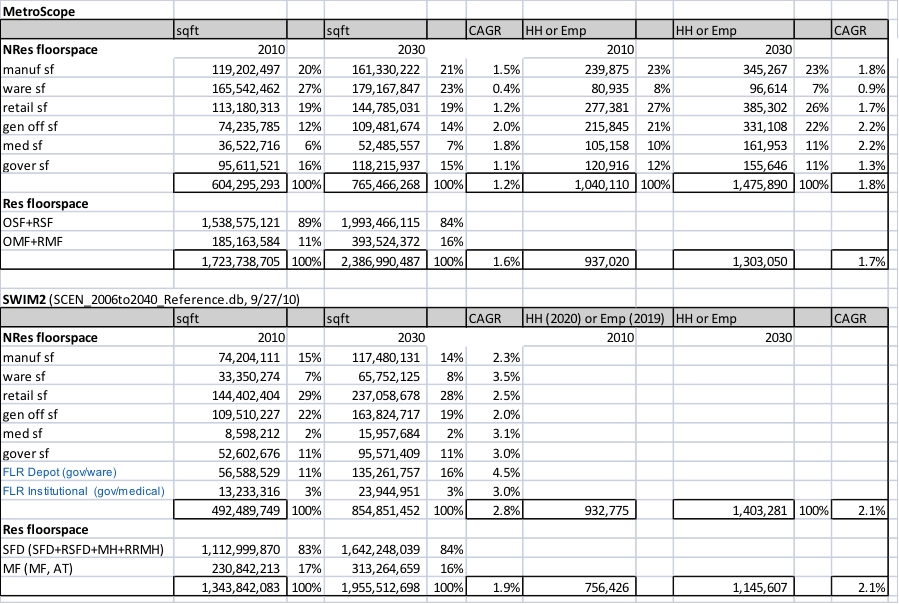
\includegraphics[width=6.5in]{ald/metroscope-comparison}
\caption{Comparison of SWIM2 versus MetroScope forecast floorspace and employment}
\label{fig:metroscope-comparison}
\end{figure}

\section{S3 parameters}
During the initial ALD S3 calibration, the three calibration steps using evolutionary algorithms were repeated using activity quantities, floorspace occupancy and price data from the S2 calibrated PI module (subsequently replaced with AA module). The ALD and AA modules were then jointly run through time to determine how well the behavior of each is affecting the other. The most important behavior of ALD with respect to the rest of the model system was that it provides an appropriate amount of increase in floorspace supply in zones where the rest of the system indicates that floorspace demand is high and little increase (or even a slight decrease) in floorspace supply in zones where the rest of the system indicates that floorspace demand is low. This appropriate response of development meeting demand was observed in initial sensitivity testing, with reasonable floorspace price increases.

The local signal for the demand for floorspace is the price of that floorspace that emerged from the PI module after PI accounts for changes in economic conditions and accessibilities. The PI module was calibrated in S2 calibration to match floorspace price distributions. In that initial S3 process no further adjustments were deemed necessary in ALD price sensitivity parameters $\beta_{4f}$ and $\beta_{6f}$ to ensure that over several years ALD responded with increased or decreased supply before prices reach unreasonable levels, particularly in zones where development capacity remains. It was noted that should the modelwide average prices or vacancy rates change unreasonably over time, $\beta_{2f}$ and $ASC_f$ parameters could also be adjusted. 

With the replacement of PI with AA and newer economic and demographic data (IMPLAN, Census), ALD may need to be tested and re-calibrated. S3 re-calibration required by recent adjustments to AA are currently on-going, and will likely need to continue to be evaluated over the life of this project.

\chapter{Activity Allocation (AA) Module}\label{sec:aa-module-chapter}
The Activity Allocation (AA) module represents the regional economic relationships among industry, households and institutions within the model. It includes the economic allocation portion of the Production, Exchange, and Consumption Allocation System (PECAS) developed by \cite{hunt05}. In each period, AA takes the aggregate modelwide activity totals (2009 dollars of production and imports/exports) from the NED module, counts of modelwide households from the SPG1 module, the available floorspace by alpha zone from the ALD module and travel accessibilities from the PT module and VISUM locates the various actors (industry and households), generates a set of economic flow matrices for each commodity and determines the technology (the commodities made and used including labor and floorspace) for each activity for each beta zone (called land use zone \textit{LUZ} in AA). AA also determines the quantity of floorspace occupied by industry and households, given a fixed floorspace supply inventory from the ALD module. 

AA labor flows are used in the SPG module to locate households (home end) and in the PT module to locate workplaces (work end). The flow of goods (including imports and exports) is used by the CT module. These uses are employed in the current year, while ALD uses AA allocation of demand in the prior two years to allocate regional construction dollars among 15 regions and prior year vacancy rates and prices to identify the floorspace types and zonal location for such development. A future Economic Feedback (EF) module will makes use of the overall quality of industry operations (AA logsums) to influence the NED regional forecast totals in the next year. Finally, the previous year AA-generated location of activities influences current-year AA activity location decisions.

AA also runs once before the base year as part of the bootstrap process. This run is constrained to reproduce observed activity distributions by beta zone. It writes constants to the ActivityLocations file that modify the behavior of AA in later years. The constrained run helps incorporate influences on activity location that are hard to measure directly, so that activities are more likely to be allocated to places where they exist in real life even if the location seems unjustified economically.

The overall approach to the allocations done in the AA module was represented diagrammatically in Figure \ref{fig:make-use-summary} (page \pageref{fig:make-use-summary}). Commodities (columns) are produced and consumed (goods, services, labor, floorspace) both for the study area and for import and export. Economic actors (rows) (industries, government, households) separately account for import make and export use activities in addition to modelwide make and use.

\section{Theoretical Basis}\label{sec:aa-theoreticals}
The Activity Allocation Module (AA Module) is an aggregate representation based on spatially-disaggregated forms of extended input-output make and use tables, with variable technical coefficients.  This approach represents a specialized adaptation of a social accounting matrix. AA concerns quantities of activities, flows of commodities and markets with aggregate demands and supplies and exchange prices.

Activities are located in land use zones (LUZ or beta zone). Activities produce commodities and then transport and sell these commodities; and they also consume commodities after buying them and transporting them.  There are different types of activities, including industrial sectors, government and households. Activity quantities can be measured in values (for example, dollars of business repair industrial activity) or numbers (for example, number of households with high income and 2 or less persons). The AA Module allocates the study-area wide quantity of each activity among the beta zone as part of its allocation process.

Commodities flow at specific rates from where they are produced to where they are exchanged (from seller to buyer), and then from where they are exchanged to where they are consumed. Commodities are grouped into categories, including different types of goods and services, labor and space. Commodities other than floorspace in general flow across zone boundaries. Floorspace is restricted in that it is ``non-transportable'' and must be exchanged and consumed in the beta zone where it is produced, which means that the space commodity categories receive some special additional treatments in PECAS.  Commodity flows are measured in values per unit time (for example, dollars of management services per year) or numbers per unit time (for example, tons of coal per month). The movement of these flows of commodities from where they are produced to where they are consumed is the economic basis for travel and transport in the modeling system.  It is the travel conditions --- the distances, costs, times and associated (dis)utilities by mode --- for the movement of these commodities that results in the influence of the transportation system on the interactions among activities and the attractiveness of locations for activities.  The AA Module allocates the flows of commodities from production location beta zone to exchange location beta zone and from exchange location beta zone to consumption location beta zone, and finds the corresponding set of prices at the exchange location beta zone that clears all markets, as part of its allocation process.

Activities produce commodities and consume commodities in the production process according to the technology they use.  More specifically, an activity quantity in a given beta zone produces commodities at specific rates per unit of activity and consumes commodities at specific rates per unit of activity according to the technology being used by the activity. One or more ``technology option'' alternatives are defined for a given activity (industry or household). Each of these technology options is a specific vector of production and consumption rates for different commodities per unit of the activity, representing a particular technology option for the production process available to the activity. The AA Module allocates the quantity of the activity in each beta zone among these ``technology options'' as part of its allocation process.

The allocation process in the AA Module uses a three-level nested logit model with a nesting structure as shown in Figure \ref{fig:aa-nesting-structure}.

\begin{figure}[!t]
\centering
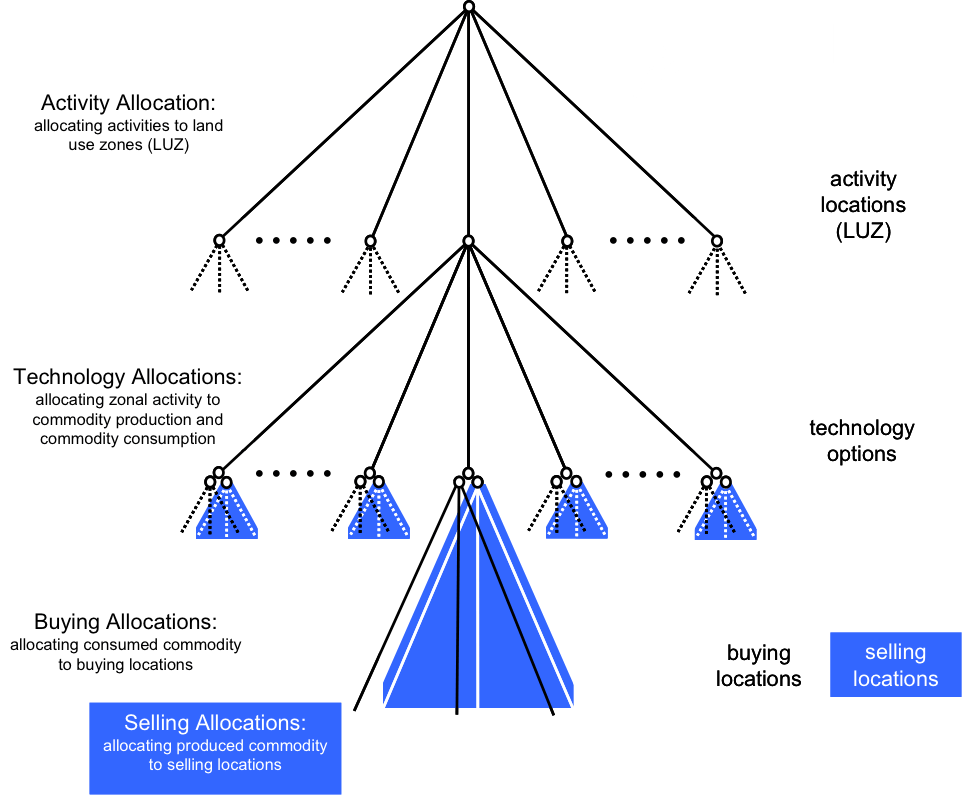
\includegraphics[scale=0.45]{aa/nesting-structure}
\caption{Three-level nesting structure used in allocations }\label{fig:aa-nesting-structure}
\end{figure}

At the highest level of the nesting structure, the study-area total quantity of each activity is allocated among the beta zone. At the middle level, the quantity of each activity in each beta zone is allocated among the available technology options. At the lowest level, there are two logit allocations for each commodity in each beta zone: The first is an allocation of the produced quantities among the various exchange locations where they are sold to other activities; the second is an allocation of the consumed quantities among the various exchange locations where they are bought by other activities.

At the lowest level, the utility of each exchange location alternative is influenced by the price at the exchange location and the characteristics for transporting the commodity to or from the exchange location.  The composite utility values from these two lowest-level logit models are called the ``buying utility'' and the ``selling utility'' for the commodity in the beta zone. They are used as the transportation-related inputs in the middle-level for allocating the activities in the beta zone among the relevant technology options. The composite utility value for the range of technology options considered at the middle-level for an activity in a beta zone is part of the location utilities used at the highest-level.

The spatial aspects of the AA Module allocation process are illustrated in Figure \ref{fig:aa-spatial-aspects}. Buying and selling allocations link through the exchange locations to establish commodity flows from production to consumption locations in the beta zone.

\begin{figure}   % Originally Figure 6.2
\centering
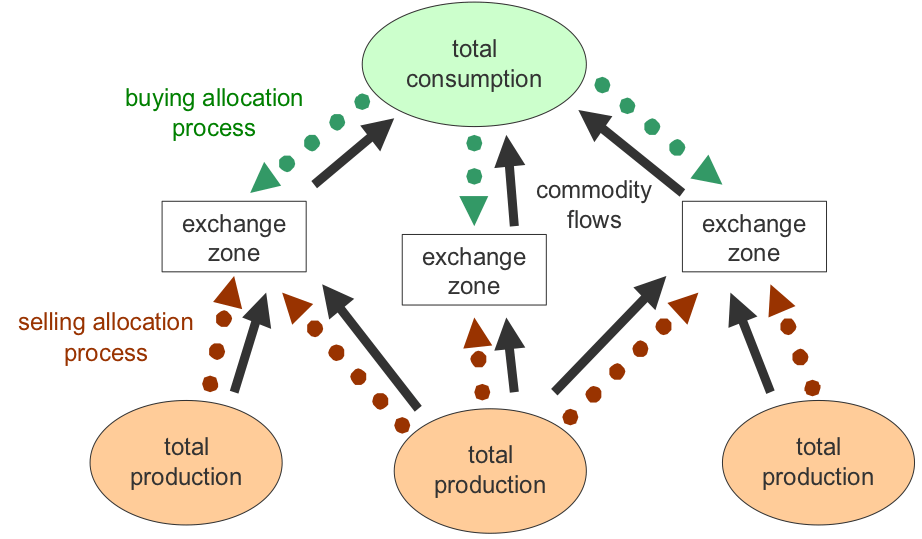
\includegraphics[scale=0.35]{aa/spatial-aspects}
\caption{Buying and selling allocations resulting in commodity flows}\label{fig:aa-spatial-aspects}
\end{figure}

The exchange locations are location-specific markets for commodities, where sellers sell commodities to buyers. Prices are established at exchange locations so that the quantity bought equals the quantity sold. Thus, the spatial allocation procedure in the AA Module assumes a short-run market equilibrium in commodities.

In the general case, commodities can be assigned in any of the available exchange zones (either all the zones in the model or a specified set of 1 or more exchange zones). For simplicity and realism, commodities can be assigned to be either (a) purchased from the exchange location in the beta zone where they are consumed (e.g. for labor, this occurs in the employment zone, where the labor is exchanged and the price set), or (b) purchased in the exchange location in the beta zone where they are produced (e.g. for retail goods this is at the retail establishment, where the goods are exchanged and the price is set), or (c) produced, exchanged and consumed in the same zone (e.g. for floorspace which is attached to the ground and cannot be moved). In these cases for each commodity in each zone, one (or both) of the logit allocation models (either the buying or the selling) consists of only one alternative.

The import and export of goods commodities that are physically transported by vehicles enter the system at six specific external exchange locations termed World Markets. The import and export quantity at each external World Market and internal exchange location are determined as functions of the exchange price in both locations, so that as prices rise more imports are attracted and as prices fall more exports are produced. The import and export functions tie the economy in the model to the rest of the world.

\section{Quantity Definitions and Categories}

AA operates at the beta zone level, although some outputs are expanded to the alpha zone level (see Figure \ref{fig:swim2-model-area} on page \pageref{fig:swim2-model-area}) for use in the SPG2 and PT modules. For import and export of goods commodities, AA uses a set of six world market zones, which are allocated to 12 external stations in the CT modules for network assignment. World markets were defined in Table \ref{tab:world-markets} and mapped in Figure \ref{fig:world-markets}. % and \ref{figure_2.4}.

AA uses the industry and household activity categories of Table \ref{tab:activity-industry} and \ref{tab:size-income} and goods, services, labor and floorspace commodity categories defined in Tables \ref{tab:service-categories} through \ref{tab:goods-categories} (pages \pageref{tab:activity-industry}--\pageref{tab:goods-categories}). Additional actors are used only in the AA and NED modules to complete the accounting of money flows. These include aspatial money flow government activities: FGOV\_acct\_gov, SLGOV\_acct\_gov, CAP\_acct\_gov, and associated aspatial activities in the eduction, investment and energy permitting sectors.

The commodity flows associated with these activities do not interact with the transportation system and have zero transport costs (money moves for free), so they are exchanged in only one zone (assumed at the alpha zone location of the state capital in Salem, OR) and do not add to the runtime of the software. For instance, ``Education reports to sponsors'' was added to track the funding of schools by governments and the responsibilities of schools to serve not only the students but also their funders. (The education flow of students going to school to be taught was renamed to ``Teaching K12'' to make it distinct from the flow of funding.)  Some inputs exist to allow GHG Permits (Greenhouse Gas Permits) to be added to the model in a future version, to support scenarios designed to understand the effect of an imposed price or cap on greenhouse gas emissions. The full set of aspatial financial flows includes:
\begin{itemize}
\item Education Reports to Sponsors,
\item Government Support Receipts
\item Tax Receipts,
\item Investing Receipts, 
\item Return Investment Receipts,
\item Capital Transfer Receipts,
\item Proprietor Income Receipts,
\item GHG Permits (Greenhouse Gas Permits) (not included in the current version)
\end{itemize}

\section{Component Models}

The objective of the AA module is to find a market clearing price equilibrium solution to a series of activity allocation equations, including the following components. These components are detailed in the remainder of this section.
\begin{itemize}
\item Production Activity allocation (modelwide)
\item Production and consumption allocation (technology)
\item Production and consumption quantities (exchange locations)
\item Imports and exports
\item Floorspace Imports
\item Equilibrium Solution
\item P-Processor Integration
\end{itemize}

\subsection{Production Activity Allocation (modelwide)}\label{sec:aa-pa-allocation-modelwide}
The ``highest'' level AA module allocates activities to zones consistent with the ``middle'' level technology assumptions (\S\ref{sec:aa-pca-technology}) and ``lowest'' level's transportation assumptions. The modelwide total quantity of production activity for each activity category is input to the AA module, per outputs from the NED (industry dollars) and SPG (households) modules. This amount is allocated in the ``highest'' level model among the Beta zones using a logit allocation as follows. The utility is sensitive to the composite utilities (CUProd and CUCons) from the ``middle'' level AA module (see \S\ref{sec:aa-pca-technology}):
\begin{equation}\label{eq:6.01}
W_{a,z} = TW_a \cdot \left[ exp(\lambda_{l,a} \cdot LU_{a,z}) / \sum_{z \in Z} exp(\lambda_{l,a} \cdot LU_{a,z}) \right]
\end{equation}
\noindent with:
\begin{equation}\label{eq:6.02}
\begin{aligned}
LU_{a,z} = {} & \alpha_{size,a} \times 1/\lambda_{l,a} \cdot ln(Size_{a,z}) + \alpha_{inert,a} \times ln(PrevW_{a,z} + InertCons_a) + \\
& Constant_{a,z} + \sum_{v \in V} (\alpha_{a,v} \cdot X_{v,z}) + \alpha_{tech,a} \cdot CUTech_{a,z}
\end{aligned}
\end{equation}
\noindent where:
\begin{align*}
z &= \text{index representing zones} \\
Z &= \text{the set of all zones} \\
a &= \text{index representing activity categories} \\
c &= \text{index representing commodity categories} \\
LU_{a,z} &= \text{location utility for a unit of activity $a$ in zone $z$} \\
W_{a,z} &= \text{quantity of activity $a$ in zone $z$} \\
TW_a &= \text{model-wide total quantity of activity $a$} \\
\lambda_{l,a} &= \text{utility function dispersion parameter for allocation of} \\
 &~~~~~\text{activity $a$ among location zones} \\
Size_{a,z} &= \text{representation of relative size of zone $z$ for activity $a$,} \\
 &~~~~~\text{indicating the a priori expected share of activity $a$ for zone $z$} \\
\alpha_{size,a} &= \text{utility function coefficient for the sensitivity to size} \\
 &~~~~~\text{for activity $a$} \\
PrevW_{a,z} &= \text{the proportion of model-wide quantity of activity $a$ in} \\
 &~~~~~\text{zone $z$ in the previous time period} \\ 
InertCons_a &= \text{Coefficient modifying the sensitivity to the previous portion} \\
 &~~~~~\text{of activity $a$ in zones, that reduces the importance of the quantity} \\
 &~~~~~\text{when the previous quantity is small} \\
\alpha_{inert} &= \text{utility function coefficient for the sensitivity to the} \\
 &~~~~~\text{previous proportion of activity $a$ in zone $z$, representing inertia in} \\
 &~~~~~\text{allocation of activity $a$} \\
Constant_{a,z} &= \text{utility function alternative specific constant for zone $z$} \\
 &~~~~~\text{for allocation of activity $a$} \\
v &= \text{index representing ``other'' zonal attributes} \\
V &= \text{the set of all ``other'' zonal attributes} \\
X_{v,z} &= \text{one of the ``other'' zonal attributes} \\
\alpha_{a,v} &= \text{utility function coefficient for the sensitivity to the} \\
 &~~~~~\text{``other'' zonal attribute} ~X_{v,z} \\
CUTech_{a,z} &= \text{composite utility associated with the range of technology options} \\
 &~~~~~\text{for activity $a$ in zone $z$, defined in equation \ref{eq:6.07} and discussed below} \\
\alpha_{tech,a} &= \text{utility function coefficient for the sensitivity to composite} \\
 &~~~~~\text{utility associated with range of technology options for activity $a$}
\end{align*}

The types of ``other'' zonal attributes in \ref{eq:6.02} that are considered to vary depending on the production activity being allocated. For residential activities in particular, these ``other'' attributes include representations of various amenities relevant to housing location choice, such as school quality, general noise levels, air quality, open space density, municipal taxation levels and possibly zonal-level income distributions and racial compositions.  In the current implementation of the PECAS software, the influences of these other zonal attributes on location utilities are incorporated by calculating the contribution to location utility in a separate process and then adding this contribution to the location utility constant ($Constant_{a,z}$).

The floorspace allocation size term $Size_{a,z}$ in \ref{eq:6.02} is normally not used (set to 1.0) because size terms representing the amount of space available to the activity in the zone $z$ are implicit in the $CUTech_{a,z}$ function (through ftsizep,a,z, see below). In the case of activities that do not explicitly use floorspace (e.g., construction industries), these size terms can be calculated and used based on other inputs (for example the amount of construction in the zone) or the quantity of relevant space so that activities are attracted to space without explicitly consuming it (see discussion of the ActivitySizeTermsI.csv file). Table \ref{tab:floorspace-consumption-rates} (page \pageref{tab:floorspace-consumption-rates})shows the category of space used each industry activity (one-to-one mapping).

\subsection{Production and Consumption Allocation (technology)}\label{sec:aa-pca-technology}
The AA Module allocates the quantity of each activity in each beta zone among the available technology options using a logit allocation as follows:
\begin{equation}\label{eq:6.03}
Tech_{p,a,z} = W_{a,z} \cdot (exp(\lambda_{p,a} \cdot UTech_{p,a,z}) \ldots
\end{equation}
\noindent with:
\begin{equation}\label{eq:6.04}
UTech_{p,a,z} = 1/\lambda_{p,a} \cdot ln(OpWeight_{p,a} \cdot ftsize_{p,a,z}) + UProd_{p,a,z} + UCons_{p,a,z}
\end{equation}
\begin{equation}\label{eq:6.05}
UProd_{p,a,z} = \ldots Rate_{p,a,n} \cdot Scale_{p,a,n} \cdot CUSell_{cn,z}
\end{equation}
\begin{equation}\label{eq:6.06}
UCons_{p,a,z} = \ldots -Rate_{p,a,n} \cdot Scale_{p,a,n} \cdot CUBuy_{cn,z}
\end{equation}
\noindent where:
\begin{align*}
p &= \text{index representing technology options} \\
P_a &= \text{the set of all technology options available for activity $a$} \\
UTech_{p,a,z} &= \text{technology utility for a unit of activity $a$ in zone $z$ applying technology} \\
 &~~~~~\text{option $p$} \\
Tech_{p,a,z} &= \text{quantity of activity $a$ in zone $z$ applying technology option $p$} \\
\lambda_{p,a} &= \text{utility function dispersion parameter for allocation of activity $a$ among} \\
 &~~~~~\text{technology options} \\
OpWeight_{p,a} &= \text{representation of relative size of application of technology option $p$ for activity} \\
 &~~~~~\text{$a$, indicating the a priori expected share of application of technology option $p$} \\
&~~~~~\text{by activity $a$} \\
UProd_{p,a,z} &= \text{the component of utility arising for a unit of activity $a$ in zone $z$ with} \\
 &~~~~~\text{production of commodities for technology option $p$} \\
UCons_{p,a,z} &= \text{the component of utility arising for a unit of activity $a$ in zone $z$ with} \\
 &~~~~~\text{consumption of commodities for technology option $p$} \\
n &= \text{index representing technical coefficients} \\
N_p &= \text{the set of technical coefficients for technology option $p$} \\
Rate_{p,a,n} &= \text{the rate at which commodity $c$ is produced (if positive) or consumed} \\
 &~~~~~\text{(if negative) by activity $a$ using technology option $p$} \\
Scale_{p,a,n} &= \text{scaling factor for the utility of} ~Rate_{p,a,n} \\ 
cn &= \text{Commodity associated with $n$} \\
CUSell_{c,z} &= \text{composite utility associated with selling a unit of commodity $c$ produced} \\
 &~~~~~\text{in zone $z$, defined in equation \ref{eq:6.14} and discussed below} \\
CUBuy_{c,z} &= \text{composite utility associated with buying a unit of commodity $c$ consumed} \\
 &~~~~~\text{in zone $z$, defined in equation \ref{eq:6.18} and discussed below} \\
ftsize_{p,a,z} &= \text{proportion of floorspace relevant to technology option $a$ (the floorspace type} \\
 &~~~~~\text{that is used by $a$) that exists in zone $z$, see size term calculation document} \\
 &~~~~~\text{for further details}
\end{align*}
        
The composite utility associated with applying the range of technology options for activity $a$ in zone z is determined consistent with equations \ref{eq:6.03} and \ref{eq:6.04} as follows:
\begin{equation}\label{eq:6.07}
CUTech_{a,z} = 1/\lambda_{p,a} \cdot ln \left[ \sum_{p \in P_a} exp(\lambda_{p,a} \cdot UTech_{p,a,z}) \right]
\end{equation}

The composite utility for the range of technology options, $CUTech_{a,z}$, includes the utilities for buying, $CUBuy_{c,z}$, and for selling, $CUSell_{c,z}$, the individual commodities that are used and made with those technology options. That is, for each technology option, Equations \ref{eq:6.05} and \ref{eq:6.06} sum the utilities $CUBuy_{c,z}$ and $CUSell_{c,z}$ with weights indicating the rates at which they are used, $ConsRate_{p,a,n}$, and made, $ProdRate_{p,a,n}$, as well as any scaling factors $Scale_{p,a,n}$ to establish the utilities for consumption, $UCons_{p,a,,z}$, and production, $UProd_{p,a,z}$, for that technology option. Equation \ref{eq:6.04} combines these utilities for consumption and production with a size term to establish the utility for that technology option, UTechp,a,z. Equation \ref{eq:6.07} then combines these utilities for the range of technology options to establish the composite utility for the range of technology options, $CUTech_{a,z}$.

The utilities for buying, $CUBuy_{c,z}$, and for selling, $CUSell_{c,z}$, reflect the accessibilities to the commodities.  Thus, the composite utility for the range of technology options, $CUTech_{a,z}$, combines the accessibilities for buying and selling individual commodities consistently with the technology (production and consumption) options for the activity. The location utility (determined in equation \ref{eq:6.02}) of an activity that consumes a large amount of a commodity will be strongly influenced by the composite utility of buying that commodity, and the location utility of an activity that produces a large amount will be strongly influenced by the composite utility of selling. As such, the last term in equation \ref{eq:6.02}, $CUTech_{a,z}$, provides overall indications of the accessibility of the zone for the activity consistent with the range of technologies applied by the activity in that zone.

\subsection{Production and Consumption Quantities (exchange locations)}\label{sec:aa-production-consumption-locations}

The quantity of commodity $c$ produced in zone $z$ by activity $a$ is the sum of the quantities of commodity $c$ produced by each technology option over the set of technology options applied by activity $a$, as follows:
\begin{equation}\label{eq:6.08}
TPA_{c,a,z} = \sum_{p \in P_a} \sum_{n \in P_a | rate(p,a,n)>0, cn=c} Rate_{p,a,n} \cdot Tech_{p,a,z}
\end{equation}

\noindent where ${TPA}_{c,a,z}$ is the quantity of commodity $c$ produced by activity $a$ in zone $z$ using all technology options (in software: ZonalMakeUse(Amount when Activity=a, MorU=M, ZoneNumber=z).

The quantity of commodity $c$ produced in zone $z$ by all activities is the sum of the quantities of commodity $c$ produced over the set of activities, as follows:
\begin{equation}\label{eq:6.09}
TP_{c,z} = \sum_{a \in A} TPA_{c,a,z}
\end{equation}
\noindent where $TP_{c,z}$ is the quantity of commodity $c$ produced by all activities in zone $z$ using all technology options. Similarly, the quantity of commodity $c$ consumed in zone $z$ by activity $a$ is the sum of the quantities of commodity $c$ consumed by each technology option over the set of technology options applied by activity $a$, as follows:
\begin{equation}\label{eq:6.10}
TCA_{c,a,z} = \sum_{n \in N} -Rate_{p,a,n} \cdot Tech_{p,a,z}, \;\; N = \{P_a | rate(p,a,n)<0, cn=c\}
\end{equation}

\noindent where $TCA_{c,a,z}$ is the quantity of commodity $c$ consumed by activity $a$ in zone $z$ using all technology options (in software: ZonalMakeUse(Negative of Amount when Activity=a, MorU=M, ZoneNumber=z).

The quantity of commodity $c$ consumed in zone $z$ by all activities is the sum of the quantities of commodity $c$ consumed over the set of activities, as follows:
\begin{equation}\label{eq:6.11}
TC_{c,z} = \sum_{a \in A} TCA_{c,a,z}
\end{equation}

\noindent where $TC_{c,z}$ is the quantity of commodity $c$ consumed by all activities in zone $z$ using all technology options.

\subsubsection{Buying and Selling Allocation}
The AA Module allocates the total quantity of each commodity produced in a given beta zone among the exchange locations (where it is sold) using a logit allocation as follows:
\begin{equation}\label{eq:6.12}
S_{c,z,k}  =  TP_{c,z} \cdot \left[ exp(\lambda_{S_c} \cdot SU_{c,z,k} ) / \sum_{k \in K} exp(\lambda_{S_c} \dot SU_{c,z,k}) \right]
\end{equation}
\noindent with:
\begin{equation}\label{eq:6.13}
SU_{c,z,k} = \delta s_{size,c} \cdot 1/\lambda_{S_c} \cdot ln(XsSize_{c,k}) + \delta s_{price,c} \cdot Price_{c,k} + \delta s_{tran,c} \cdot Tran_{c,z,k}
\end{equation}
\noindent where:
\begin{align*}
k &= \text{index representing exchange locations (LUZ)} \\
K &= \text{the set of all exchange locations} \\
S_{c,z,k} &= \text{quantity of commodity $c$ produced in zone $z$ allocated to be sold in exchange} \\
 &~~~~~\text{location $k$ (hence is shipped from zone $z$ to exchange location $k$)} \\
SU_{c,z,k} &= \text{utility for selling in exchange location $k$ a unit of commodity $c$ produced in} \\
 &~~~~~\text{zone $z$} \\
XsSize_{c,k} &= \text{representation of relative size of exchange location $k$ for selling commodity $c$,} \\
 &~~~~~\text{indicating the a priori expected share of commodity $c$ sold in exchange} \\
 &~~~~~\text{location $k$} \\
Price_{c,k} &= \text{the unit exchange price for commodity $c$ in exchange location $k$} \\ 
Tran_{c,z,k} &= \text{the utility for transporting a unit of commodity $c$ from zone $z$ to exchange} \\
 &~~~~~\text{location $k$, as calculated in equation \ref{eq:6.20} below} \\
\delta s_{size,c} &= \text{utility function coefficient for the sensitivity to size when selling commodity $c$} \\
\delta s_{price,c} &= \text{utility function coefficient for the sensitivity to price when selling commodity $c$} \\
\delta s_{tran,c} &= \text{utility function coefficient for the sensitivity to transport utility when selling} \\
 &~~~~~\text{commodity $c$} \\
\lambda s_c &= \text{utility function dispersion parameter for allocation of selling of commodity $c$}
\end{align*}

In the case of selling, the coefficient $\delta s_{price,c}$ is positive.

The selling composite utility for commodity $c$ (independent of the producing activity) is determined consistent with equations \ref{eq:6.12} and \ref{eq:6.13} as follows:
\begin{equation}\label{eq:6.14}
CUSell_{c,z} = 1/\lambda s_c \cdot ln \left[ \sum_{k \in K} exp(\lambda s_c \cdot SU_{c,z,k}) \right]
\end{equation}

\noindent where: $CUSell_{c,z}$ is the composite utility associated with selling a unit of commodity $c$ produced in zone $z$, independent of activity (in software: CommodityZUtilities(zUtility) when BuyingOrSelling=S).

The AA Module allocates the total quantity of each commodity consumed among the exchange zones in a manner that is analogous to the allocation of produced quantities. Specifically, the total quantity of each commodity consumed in a given LUZ is allocated among the exchange locations (where it is bought) using a logit allocation as follows:
\begin{equation}\label{eq:6.16}
B_{c,z,k} = TC_{c,z} \cdot \left[ exp(\lambda b_c \cdot BU_{c,z,k}) / \sum_{k \in K} exp(\lambda b_c \cdot BU_{c,z,k}) \right]
\end{equation}
\noindent with:
\begin{equation}\label{eq:6.17}
BU_{c,z,k} = \delta b_{size,c} \cdot 1/\lambda b_c \cdot ln(XbSize_{c,k}) + \delta b_{price,c} \cdot Price_{c,k} + \delta b_{tran,c} \cdot Tran_{c,k,z}
\end{equation}
\noindent where:
\begin{align*}
B_{c,z,k} &= \text{quantity of commodity $c$ consumed in zone $z$ allocated to be bought in} \\
 &~~~~~\text{exchange location $k$ (hence is shipped from exchange location $k$ to zone $z$)} \\
BU_{c,z,k} &= \text{utility for buying in exchange location $k$ a unit of commodity $c$ consumed} \\
 &~~~~~\text{in zone $z$} \\
XbSize_{c,k} &= \text{representation of relative size of exchange location $k$ for buying commodity} \\
 &~~~~~\text{$c$, indicating the a priori expected share of commodity $c$ bought in exchange} \\
 &~~~~~\text{location $k$} \\
Tran_{c,k,z} &= \text{the utility for transporting a unit of commodity $c$ from exchange location $k$} \\
 &~~~~~\text{to zone $z$, as calculated in equation \ref{eq:6.20} below} \\
\delta b_{xsize,c} &= \text{utility function coefficient for the sensitivity to size when buying} \\
 &~~~~~\text{commodity $c$} \\
\delta b_{price,c} &= \text{utility function coefficient for the sensitivity to price when buying} \\
 &~~~~~\text{commodity $c$} \\
\delta b_{tran,c} &= \text{utility function coefficient for the sensitivity to transport utility when buying} \\
 &~~~~~\text{commodity $c$} \\
\lambda b_c &= \text{utility function dispersion parameter for allocation of buying of commodity $c$}
\end{align*}

In the case of buying, the coefficient $\delta b_{price,c}$ is negative.

The buying composite utility for commodity $c$ (independent of the consuming activity) is determined consistent with equations \ref{eq:6.16} and \ref{eq:6.17} as follows:
\begin{equation}\label{eq:6.18}
CUBuy_{c,z} = (1/\lambda b_c) \cdot ln \left[ \sum_{k \in K} exp(\lambda b_c \cdot BU_{c,z,k}) \right]
\end{equation}
\noindent where $CUBuy_{c,z}$ is the composite utility associated with buying a unit of commodity $c$ consumed in zone $z$, independent of activity. 

The utility for transporting a unit of commodity $c$ from any zone $j$ to any zone $k$, $Tran_{c,j,k}$, is calculated using up to a maximum of three interchange attribute values (that are provided by the transit assignment module) as follows:
\begin{equation}\label{eq:6.20}
Tran_{c,j,k} = \kappa 1_c \cdot IntAtt1_{j,k} + \kappa 2_c \cdot IntAtt2_{j,k} + \kappa 3_c \cdot IntAtt3_{j,k}
\end{equation}
\noindent where:
\begin{align*}
IntAtt1_{j,k} &= \text{value for attribute 1 from land use zone $j$ to land use zone $k$ used} \\
 &~~~~~\text{to calculate the utility for transporting a unit of commodity $c$} \\
IntAtt2_{j,k} &= \text{value for attribute 2 from land use zone $j$ to land use zone $k$ used} \\
 &~~~~~\text{to calculate the utility for transporting a unit of commodity $c$} \\
IntAtt3_{j,k} &= \text{value for attribute 3 from land use zone $j$ to land use zone $k$ used} \\
 &~~~~~\text{to calculate the utility for transporting a unit of commodity $c$} \\
\kappa 1_c &= \text{utility function coefficient for the sensitivity to attribute 1 when transporting} \\
 &~~~~~\text{a unit of commodity $c$} \\
\kappa 2_c &= \text{utility function coefficient for the sensitivity to attribute 2 when transporting} \\
 &~~~~~\text{a unit of commodity $c$} \\
\kappa 3_c &= \text{utility function coefficient for the sensitivity to attribute 3 when transporting} \\
 &~~~~~\text{a unit of commodity $c$}
\end{align*}

An ``exchange regime'' is specified for each commodity $c$. This exchange regime indicates the spatial nature of the exchanges available for the commodity. For example, some commodities are only exchanged where they are produced. Thus, the exchange zone must be the zone of production. The exchange regime for each commodity $c$ is designated using single-letter code for the variable $ExChc$ as follows:
\begin{align*}
\text{`c'} &= \text{exchanged only in consumption zones (where the seller does all transporting)} \\
\text{`p'} &= \text{exchanged only in production zones (where the buyer does all transporting)} \\
\text{`a'} &= \text{exchanged in any zone (where either buyer and seller may do the transporting)} \\
\text{`n'} &= \text{non-transportable (where the commodity is consumed in the same zone where it} \\
 &~~~~~\text{is produced)} \\
\text{`s'} &= \text{exchanged only in specified zones (both buyer and seller may do some of the} \\
 &~~~~~\text{transporting, but exchanges occur in only certain zones)}
\end{align*}

In the Oregon implementation of AA the following transport-related travel attributes ($IntAtt_{j,k}$) are used as defaults: For labor flows (commuting) the mode choice logsums from the prior year PT run are used. For goods commodities, distance, time and toll skims are used (from prior year traffic assignment). Goods are typically type `p' or `a', labor are type `c' and floorspace is type `n'.

\subsection{Imports and Exports}\label{sec:aa-import-export}
The quantities of imports and exports for a given commodity in a given exchange zone are determined using:
\begin{equation}\label{eq:6.21}
Q_{c,i,k} = QRef_{c,i}  + \Delta_{c,i} \times ([G_i-1]/[G_i+1]) + \mu_{c,i} \times (Price_{c,k} - PriceRef_{c,i})
\end{equation}
\begin{equation}\label{eq:6.22}
Q_{c,e,k}  = QRef_{c,e} + \Delta_{c,i} \times ([G_e-1]/[G_e+1]) + \mu_{c,e} \times (Price_{c,k} - PriceRef_{c,e})
\end{equation}
\noindent with:
\begin{equation}\label{eq:6.23}
G_i = exp(\eta_{c,i} \times (Price_{c,k} - PriceRef_{c,i}))
\end{equation}
\begin{equation}\label{eq:6.24}
G_e = exp(\eta_{c,e} \times (Price_{c,k} - PriceRef_{c,e}))
\end{equation}
\noindent where:
\begin{align*}
Q_{c,i,k} &= \text{quantity of commodity $c$ imported to exchange location $k$} \\ 
Q_{c,e,k} &= \text{quantity of commodity $c$ exported from exchange location $k$} \\ 
QRef_{c,i} &= \text{quantity of commodity $c$ imported to exchange location when the unit exchange} \\
 &~~~~~\text{price for commodity $c$ in exchange zone $k$ is at its import reference level} ~PriceRef_{c,i} \\ 
QRef_{c,e} &= \text{quantity of commodity $c$ exported from exchange location when the unit exchange} \\
 &~~~~~\text{price for commodity $c$ in exchange zone $k$ is at its export reference level} ~PriceRef_{c,e} \\
PriceRef_{c,i} &= \text{reference price per unit for import of commodity $c$} \\ 
PriceRef_{c,e} &= \text{reference price per unit for export of commodity $c$} \\ 
Price_{c,k} &= \text{unit exchange price for commodity $c$ in exchange location $k$ (equation \ref{eq:6.13})} \\ 
\Delta_{c,i} &= \text{function coefficient for the rate of increase in imports of commodity $c$ for} \\
 &~~~~~\text{exponent term} \\ 
\mu_{c,i} &= \text{function coefficient for the rate of increase in imports of commodity $c$ for linear term} \\ 
\eta_{c,i} &= \text{function coefficient for sensitivity to difference in exchange price for commodity} \\
 &~~~~~\text{$c$ concerning increase in imports of commodity $c$ for exponent term} \\ 
\Delta_{c,e} &= \text{function coefficient for the rate of increase in exports of commodity $c$ for} \\
 &~~~~~\text{exponent term} \\ 
\mu_{c,e} &= \text{function coefficient for the rate of increase in exports of commodity $c$ for linear term} \\ 
\eta_{c,e} &= \text{function coefficient for sensitivity to difference in exchange price for commodity} \\
 &~~~~~\text{$c$ concerning increase in exports of commodity $c$ for exponent term} 
\end{align*}






In the case of imports, the coefficient $\Delta_{c,i}$ is positive and the coefficient $\mu_{c,i}$ is positive provided $\eta_{c,i}$ is positive. In the case of exports, the coefficient $\Delta_{c,e}$ is negative and the coefficient $\mu_{c,e}$ is negative provided $\eta_{c,e}$ is positive.

In the current implementation of the model, this abstract treatment of imports and exports in each exchange zone is mostly forgone in favor of an explicit representation of importing and exporting activities which are constrained to locate in the world market zones surrounding the region.

\subsection{Floorspace Imports}\label{sec:aa-floorspace-imports}
The supply of floorspace in each zone by floorspace type is treated as an ``import.''  Floorspace is not a true import, but can be treated as an import in the sense that it has a fixed short-term supply calculated separately in the ALD module. Short-term floorspace import functions in the form of equation \ref{eq:6.21} are generated internally by AA based on the fixed short-term inventory of physical space established by ALD.

Floorspace import functions are used to calculate demand for floorspace by the activity in each zone considering the physical amount of floorspace inventory reported in ALD. Each floorspace import function is a short-term supply curve for floorspace of a single type and represents the tendency for portions of available floorspace inventory to be left vacant in the short-term if prices are too low. (The floorspace is supplied by landlords whose short-term behavior is represented using the same equations that are used to calculate the imports of other commodities, as shown in \S\ref{sec:aa-import-export}). 
 
The price-vacancy relationship used is shown in Figure \ref{fig:aa-floorspace-import}. It shows that at the expected price (100 percent on the x-axis), over 90 percent of the available floorspace will be used (10 percent vacant); as prices decline more and more of the space will be left vacant; if prices were to reach zero all available floorspace supply would be utilized (zero percent vacant). The chosen logistic representation of the import curve allows the amount of floorspace used in a zone to exceed 100 percent of the fixed short-term supply at very high prices (and drop below zero percent at negative prices) in order to allow the search procedure to find for more reasonable prices during AA's own price search iterations.

\begin{figure}
\centering
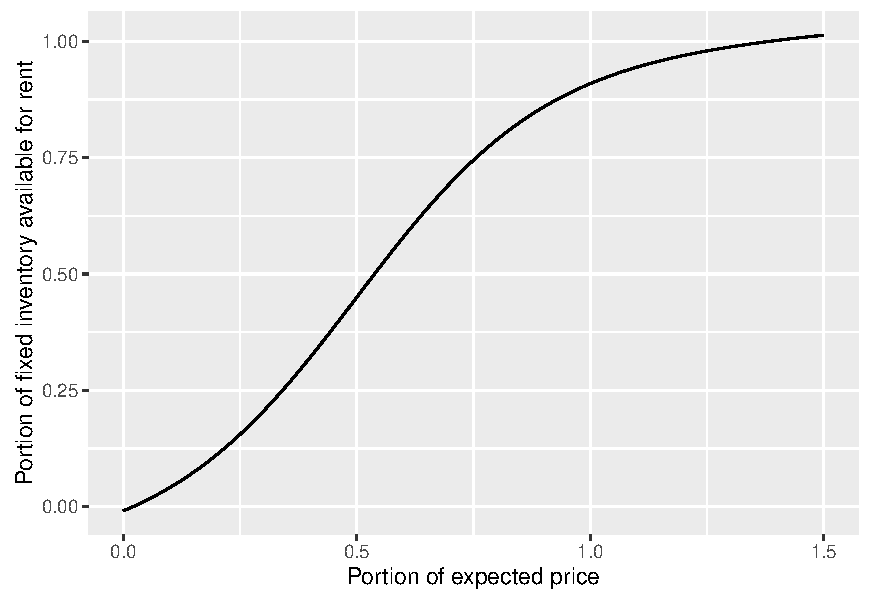
\includegraphics[scale=0.77]{aa/aa-floorspace-import-function}
\caption{Floorspace import function}\label{fig:aa-floorspace-import}
\end{figure}

The following floorspace-specific import equations are used in the AA import function(in place of the more general equations \ref{eq:6.22} through \ref{eq:6.24} used by all other imports found in \S\ref{sec:aa-import-export}):

\begin{equation}\label{eq:6.25}
PriceRef_c = \alpha_{Price, f} \times FLRPriceRef_f
\end{equation}
\begin{equation}\label{eq:6.26}
QRef_c = \alpha_{Qty,f} \times FLRQtyRef_f
\end{equation}
\begin{equation}\label{eq:6.27}
\Delta_c = \alpha_{\delta,f} \times FLRQtyRef_f
\end{equation}
\begin{equation}\label{eq:6.28}
\eta_c = \alpha_{\eta,f} / FLRPriceRef_f
\end{equation}
\begin{equation}\label{eq:6.29}
\mu_c = (\alpha_{\lambda,f} / FLRPriceRef_f) \cdot FLRQtyRef_f
\end{equation}
\noindent where:
\begin{align*}
f &= \text{index of floorspace categories} \\
FLRPriceRef_f &= \text{commodity-specific annual price (\$/Msqft) for (imported) floorspace} \\
 &~~~~~\text{(also used as a starting price for zones with no starting price)} \\
FLRQtyRef_f &= \text{current year quantity of (imported) floorspace of type $f$} \\
\alpha_{Price,f}, \alpha_{*,f} &= \text{floorspace-specific parameters to be adjusted in calibration}
\end{align*}

\subsection{Equilibrium Solution and Convergence Criteria}

The quantities of each commodity being bought and sold in each exchange zone by the activities in the model area (not imports or exports) are calculated as a sum of the buying and selling quantities solved for in the AA ``middle'' technology model (see \S\ref{sec:aa-pca-technology}), as follows:
\begin{equation}\label{eq:6.30}
TBD_{c,k} = \sum_{z \in Z} B_{c,z,k}
\end{equation}
\begin{equation}\label{eq:6.31}
TSD_{c,k} = \sum_{z \in Z} S_{c,k,z}
\end{equation}
\noindent where:
\begin{align*}
c &= \text{index of commodity} \\
k, z &= \text{index of zones, when paired indicate origin, destination zone} \\
Z &= \text{set of all model zones} \\
B_{c,z,k} &= \text{quantity of commodity $c$ consumed in zone $z$ that is allocated to} \\
 &~~~~~\text{(come from) exchange location $k$ (Buying\_\$commodity.zmx [equation \ref{eq:6.16}])} \\
S_{c,k,z} &= \text{quantity of commodity $c$ produced in zone $z$ that is allocated to (go to} \\
 &~~~~~\text{exchange location $k$ (Selling\_\$commodity.zmx (equation \ref{eq:6.12})} \\
TBD_{c,k} &= \text{total quantity of commodity $c$ being bought in exchange zone $k$ by all} \\
 &~~~~~\text{activities in the model area (ExchangeResults[InternalBought])} \\
TSD_{c,k} &= \text{total quantity of commodity $c$ being sold in exchange zone $k$ by all activities in} \\
 &~~~~~\text{the model area (ExchangeResults[InternalSold])}
\end{align*}

The quantities of each commodity being bought and sold in each exchange zone in total (by the activities in the model area as well as imports and exports) --- also called the aggregate demand and aggregate supply for commodity $c$ in exchange zone $k$ --- are calculated as follows:
\begin{equation}\label{eq:6.32}
TDem_{c,k} = Q_{c,e,k} + \sum_{z \in Z} B_{c,z,k}
\end{equation}
\begin{equation}\label{eq:6.33}
TSup_{c,k} = Q_{c,i,k} + \sum_{z \in Z} S_{c,k,z}
\end{equation}
\noindent where:
\begin{align*}
TDem_{c,k} &= \text{aggregate demand for commodity $c$ in exchange zone $k$ by all activities} \\
 &~~~~~\text{in the model area} \\ 
TSup c,k &= \text{aggregate supply for commodity $c$ in exchange zone $k$ by all activities} \\ 
 &~~~~~\text{in the model area} \\ 
Q_{c,i,k} &= \text{quantity of commodity $c$ imported to exchange location $k$} \\
Q_{c,e,k} &= \text{quantity of commodity $c$ exported from exchange location $k$} 
\end{align*}

At convergence these bought and sold amounts in a given zone, $TDem_{c,k}$  and $TSup_{c,k}$ are equal. This amount is also the referred to as the ``exchange quantity'' for the commodity in the zone:
\begin{equation}\label{eq:6.34}
TE_{c,k} = TDem_{c,k} = TSup_{c,k}
\end{equation}
\noindent where $TE_{c,k}$ is the exchange quantity for commodity $c$ in exchange zone $k$. 

Since AA solves the system using numerical methods, equation \ref{eq:6.34} is not solved exactly, but within a certain convergence tolerance. The residual commodity amount, $TSup_{c,k} - TDem_{c,k}$ is reported as output to allow user checks for appropriate convergence tolerance (ExchangeResults[Surplus]).

\subsubsection{Managing and Monitoring the Solution Algorithm}
The AA Module searches for the set of prices that establishes the equilibrium solution where all the markets clear, where the total demand minus the total supply minus the total demand for each commodity $c$ in each exchange zone $k$, denoted $Residual_{c,k}$, is zero. It performs this search in a series of iterations.

In each iteration a new set of prices is considered. The extent that the values for $Residual_{c,k}$ are not zero with these prices is evaluated and appropriate updates to these prices are calculated and applied. The process then moves to the next iteration with these prices used as the new set of prices.

This search process is managed by specifying the criteria that must be satisfied in order for the process to stop and by controlling elements of the calculation of the updates to prices in each iteration. These elements of this management are outlined below.

\subsubsection{Measuring Extent of Convergence and Specifying Stopping Rules}
In each iteration, the search process measures the extent that the values for $Residual_{c,k}$are not zero using a weighted sum-of-squares value as follows:
\begin{equation}\label{eq:6.35}
MClear = \sum_{c \in C} VergeWt_c^2 \sum_{k \in K} (Residual_{c,k})^2
\end{equation}
\noindent where:
\begin{align*}
MClear &= \text{residual-squared measure of the extent that all markets have not cleared and} \\
 &~~~~~\text{the condition that $Residual_{c,k} = 0$ for all $c$ and $k$ has not been satisfied;} \\
 &~~~~~\text{a value of 0 indicates the condition has been fully satisfied} \\
VergeW_{tc} &= \text{weight applied to residual-squared values for commodity $c$ to account for} \\
 &~~~~~~\text{units effects when summing residual-squared values across commodities} 
\end{align*}

The search process uses this value in its determination of the appropriate update to the prices for the next iteration.

The search process reports the value of $MClear$ in each iteration, by writing it to the log file. This value is influenced by the units used for the commodities and by the size of the markets considered, which can make it difficult to interpret.  A normalized form of the measure is also calculated and reported as follows:
\begin{equation}\label{eq:6.36}
TClear = \left[ \sum_{c \in C} VergeWt_c^2 \sum_{k \in K} (Residual_{c,k})^2 \right]^{0.5} /  AveExchgTotal
\end{equation}
\noindent with:
\begin{equation}\label{eq:6.37}
AveExchgTotal = \left[ \sum_{c \in C} VergeWt_c^2 \sum_{k \in K} (0.5 \cdot (TSup_{c,k} +TDem_{c,k}))^2 \right]^{0.5}
\end{equation}
\noindent where $TClear$ is the normalized measure of the extent that all markets have not cleared and the condition that $Residual_{c,k}$ = 0 for all $c$ and $k$ has not been satisfied; a value of zero indicates the condition has been fully satisfied (in software: GOF output to logfile).

$TClear$ may be much larger than 1.0 in the initial iterations of a search, but will quickly drop to much smaller values on its way to a value of zero when the search process is converging to a solution.

The search process is terminated when either (a) the values for $Residual_{c,k}$ satisfy specified convergence criteria indicating they are sufficiently close to zero, or (b) the specified maximum number of iterations is reached.

The maximum number of iterations, $Imax$, is specified in the aa.properties Run Control file using the setting for aa.maxiterations. The number of iterations required for the AA Module to converge is influenced by many factors, so it is not possible to provide definitive guidance on suitable values for $IMax$ overall. That said, in general, with convergence criteria that are reasonable and not too stringent and starting prices are not too wildly different from the solution prices, it should not take more than about 500 iterations for the AA Module to converge. Numbers of iterations well beyond that without convergence may be indicative of problems making it too difficult (and perhaps even impossible) to achieve convergence.

Two basic types of convergence criteria regarding the values for $Residual_{c,k}$are included. Both use normalized measures that are always positive and are zero at the equilibrium solution. One concerns the extent that all markets are cleared, the other concerns the extent that individual markets are cleared. Each is described below:

\subsubsection{(a) Total Clearance Criterion}
The ``total clearance'' criterion concerns the extent of market clearance for all commodities in all markets altogether, and uses the $TClear$ measure defined above. A maximum value is specified and $TClear$ must be less that this maximum value in order for the criterion to be satisfied. This maximum value is denoted $MaxTClear$, and it is specified in the aa.properties Run Control file using the setting for aa.maxTotalClearance.

In general, values of $MaxTClear$ in the range of 0.001 are used.

Further guidance on appropriate values for $MaxTClear$ can be obtained by considering the values for $MClear$ and $AveExchgTotal$ arising in a typical economy with specific total differences between supply and demand in the units being used. For example, if the units are dollars for all commodity values and all the commodity weights $VergeWtc$ are 1.0, then a combined residual of about 1000 dollars for all commodities in all zones (a comparatively small amount in most cases) would result in a value of $MClear$ of about 1e6. With a total economy of 10 billion dollars of exchanges, the value of $AveExchgTotal$ is 1e10, so the resulting value of $TClear$ is 1e-7.

The search algorithm reports the value of $TClear$ in each iteration, making it possible to monitor the progress towards satisfying the requirement that $TClear$ be less than $MaxTClear$.

\subsubsection{(b) ``Specific Clearance'' Criterion}
The ``Specific Clearance'' criterion concerns the extent of clearance for specific commodities in individual markets. It uses a measure for an individual commodity and market as follows:
\begin{equation}\label{eq:6.38}
SClear_{c,k} = | Residual_{c,k} | / SingleExchgTotal_{c,k}
\end{equation}
\noindent with:
\begin{equation}\label{eq:6.39}
SingleExchgTotal_{c,k} = | (0.5 \cdot (TSup_{c,k} +TDem_{c,k})) | + ConFac \cdot AveExchgTotal / VergeWt_c
\end{equation}
\noindent where $ConFac$ is a factor adjusting the scaled contribution to the denominator ensuring it is not zero in $SClear_{c,k}$ (in software: GOF output to logfile). A maximum value is specified and all $SClear_{c,k}$ for all $c$ and $k$ must be less than this maximum value in order for the criterion to be satisfied. This maximum value is denoted MaxSClear, and it is specified in the aa.properties Run Control file using the setting for aa.maxSpecificClearance.

In general, values of $MaxSClear$ in the range of 0.01 are used.

The value for $ConFac$ is specified in the aa.properties Run Control file using the setting for aa.contributionfactorscale. In general, a value approximately equal to the reciprocal of the number of LUZ in the model is used.

Certain $SClear$ values may be much larger than 1.0 in the initial iterations of a model run, but will quickly drop to much smaller values on their way to values of zero when the model is converging to a solution.

The search algorithm reports the maximum value of $SClear_{c,k}$ for each commodity $c$ across the set of exchange zones $k$ in each iteration, making it possible to monitor the progress towards satisfying the requirement that all the $SClear_{c,k}$ be less than $MaxSClear$.

\subsubsection{Controlling Price Update Calculation}
The updates to the prices in a given iteration are calculated seeking to minimize the value of $MClear$.

These updates to the prices are calculated by first calculating initial ``full update'' values that are then multiplied by a step size value in order to get the values that are applied in the iteration.

The initial ``full update'' in the price for each commodity in each exchange zone is the sum of (a) an adjustment calculated for an average price across all exchange zones and (b) an adjustment calculated for the local price for just that exchange zone multiplied by the a weighting factor called the Local Step Size Adjustment factor, or $StepLoc$.

The value for $StepLoc$ used in this calculation is specified in the aa.properties Run Control file using the setting for aa.localPriceStepSizeAdjustment. It can be used to adjust the relative contribution of average price change using an exact Newton's method and the local price change using a local derivative.

In general, a value of 0.5 is used for $StepLoc$.

The initial ``full update'' values obtained as described above are then multiplied by the Full Step Size Adjustment factor, Step, in order to get the ``adjusted update'' values used in the iteration.

If these adjusted update values result in a lower (better) value for $MClear$, then the software automatically increases the value of Step slightly for the next iteration. Further such increases in Step will be made, if appropriate, in subsequent iterations until a specified maximum value for Step is reached.  The search process will continue with this maximum value for Step being used as long as lower values for $MClear$ are being obtained.  If these adjusted update values results in a higher (poorer) value for $MClear$, then these values are not applied and the value of Step is reduced, and a new and smaller value of Step is used to calculate new adjusted update values to replace the abandoned ones. Further reductions to Step will be made, if required, until it reaches a specified minimum value. Iterations will continue with this minimum value until lower values for $MClear$ are being obtained.

The initial, maximum and minimum values for Step --- StepInit, StepMax and StepMin, respectively --- are specified in the aa.properties Run Control file using the settings for aa.initialStepSize, aa.maximumStepSize and aa.minimumStepSize, respectively. 

Regardless of these settings, if the current value of Step results in a numerical overflow, the value of Step is reduced even if doing so would result in it being below the specified minimum value.

A low value for StepInit, around 0.001, is appropriate, particularly in the initial stages of model development where there are larger changes being made and the starting prices are less likely to be close to the solution prices.  This allows the solution algorithm to establish an appropriate search direction before moving too much at the start.

The value for StepMin is the minimum value of Step the search process can use when encountering increases rather than decreases in $MClear$.  When the search process has been forced to use StepMin, it is still moving the direction the derivatives have indicated is the most appropriate, but is reducing the amount that it is moving because it has found that the result is not good when it moves a larger amount.  Sometimes the search process has to get ``over a hump'' before it can proceed to even lower values in the $MClear$ measure of convergence.  It will do this using the minimum value for Step.  If this minimum value is too small, then it will take a large number of iterations to get ``over the hump'', requiring large quantities of computer runtime. But the search process uses the derivatives at its current location to establish an indication of the most appropriate direction for the next iteration, and if the minimum value for Step is too large, then the solution algorithm may not be able to keep from moving beyond the range where this indication is accurate, and may then jump around ``wildly'' from one iteration to the next. A compromise value is required, usually established by trial and re-trial for each particular model. On the basis of experience a value of 0.01 for StepMin is a good place to start. 

The value for StepMax is the maximum value of Step the search process can use when encountering decreases in $MClear$. When the search process is using StepMax, it is making consistently good progress towards convergence. A value of 1.0 for Step results in the search algorithm using Newton's Method directly in the determination of the average price adjustment, which should lead to good convergence. A somewhat larger value for Step may further speed convergence. But, if a much larger value for Step is used, and the search process moves beyond the range where the indications provided by the derivatives at its current location are accurate, then the process may jump around ``wildly''. At that time, when it encounters an increase rather than a decrease in $MClear$, the algorithm will reduce the value of Step. An appropriate maximum value for Step can help avoid some of this increasing and decreasing of Step, and thereby help speed convergence. Finding an appropriate value is again a trial and re-trial process. Experience has shown that an effective strategy for helping minimize runtimes to convergence is to start with a value of 2.0 for the maximum value of Step, or even 2.0 divided by the value for the local price step size adjustment, and then keep reducing this value in subsequent model runs until there are comparatively few instances where Step is reduced from the maximum value.

At convergence, the AA model provides the following at the beta zone level prior to post-processing of some results to the alpha zone level (see \S\ref{sec:aa-p-processor}):
\begin{itemize}
\item Consistent (household and industry dollar) activity allocations by activity category by zone.
\item Commodity flow quantities from production zone to consumption zone via exchange zone.
\item Imports and exports by exchange zone.
\item Exchange prices by commodity by exchange zone. 
\end{itemize}

\subsection{P-Processor Integration}\label{sec:aa-p-processor}
To facilitate AA's interaction with other SWIM2 modules, an AA p-processor is used to both create AA input files and post-process AA output files into the appropriate format. The AA pre-processor produces the following files used as working inputs to AA. These files pull data from other SWIM2 modules and previous year AA outputs:
\begin{itemize}
\item Current year modelwide activities in the ActivityTotalsW.csv[TotalAmount] field are culled from:
\begin{itemize}
\item A base file ActivityTotalsI.csv
\item SPG1 module household counts:householdsByHHCategory.csv [spg1Households]. 
\item NED module modelwide industry/institution production activity in activity\_forecast.csv[output], government\_forecast.csv.
\item NED module modelwide imports and exports for goods commodities in trade\_forecast.csv.
\item Amount of office support activity is calculated based on the use of the office support commodities by the associated production activities. The base file TechnologyOptionsI.csv is read to determine the use rates; these are multiplied by the size of the production activities to determine total use, and divided by make rate (usually 1.0) to determine required industry size.
\end{itemize}
In the first AA run, only the NED updates and the office support update happen; households and imports/exports are read directly from the base ActivityTotalsI.csv file.

\item Current year fixed floorspace inventory in FloorspaceW.csv file, updates the current year ALD module floorspace output FloorspaceI.csv with fixed production-based quantities of agriculture and forest lands (in acres) found in the AgForestFloorspace.csv.
\item Zone-specific size terms ActivitiesZonalValuesW.csv come from:
\begin{itemize}
\item A base file ActivitiesZonalValuesI.csv if provided, otherwise the previous year zonal activity output ActivityLocations.csv[Quantity]
\item ALD output current year construction activity Increments.csv[IncMSQFT]
\end{itemize}
\item Current year technical coefficients in TechnologyOptionsW.csv are adjusted from base file TechnologyOptionsI.csv with adjustments made to industry labor use. Industry labor use rates are scaled based on the SPG to NED HHs per employees, relative to the 2009 reference year ratios (found in GlobalTemplate.properties [aa.09.productivity.rate]).
\end{itemize}

In addition to the preprocessor steps, a Python file (retexchange.py) runs before AA. This script updates ExchangeImportExportI.csv with size terms for exchange locations for commodities of the `a' type (can be exchanged in any zone). The size terms are determined based on the amount of space available for conducting the exchange (Warehouse or Retail), according to the input file ExchangeSizeTermTypes.csv.

Selected AA outputs (Table \ref{tab:aa-outputs}) are also disaggregated to the alpha zone level by the AA post-processor for use in other SWIM2 modules. Several of these AA post-processor activities are detailed below.

\subsubsection{Alpha Zone Activity and Commodity Totals}
AA works at the beta zone level and allocates modelwide activity to beta zones. The AA post-processor knows the distribution of floorspace by alpha zone from the ALD module. By assuming that, at the disaggregate level, individual units of an activity (e.g., the space required for an individual worker) only use a single floorspace type, the AA output beta zone activity totals can be allocated to alpha zones. The following formulation is used to produce alpha zone activity levels [ActivityLocations2.csv]:\footnote{A similar process is used to develop alpha zone commodity quantities (in binary and comma-separated value formats) [FloorspaceZoneTotalMakeUse.csv]. However, this file has not been fully debugged and should not be used.}
\begin{equation}\label{eq:6.40}
W_{a,\alpha} = W_{a,z} \cdot \sum_{f \in F} \left[ U_{f,a,z} / \sum_{f1 \in F} U_{f1,a,z} \right] \cdot FLR_{f,\alpha} / \sum_{\alpha 1 \in Z} FLR_{f, \alpha 1}
\end{equation}
where:
\begin{align*}
W_{a,\alpha} &= \text{amount of activity $a$ in alpha zone $\alpha$ (ActivityLocations2.csv[Quantity])} \\
W_{a,z} &= \text{amount of activity $a$ in beta zone $z$ (ActivityLocations.csv[Quantity])} \\
U_{f,a,z} &= \text{amount of floorspace commodity $f$ consumed per unit of activity $a$ in} \\
 &~~~~~~\text{beta zone $z$ (MakeUseW[marginal] and [discretionary]} \\
F &= \text{set of floorspace types used by activity $a$ in beta zone $z$} \\
FLR_{f,\alpha} &= \text{amount of floorspace type $f$ in $\alpha$ (FloorspaceW.csv[BldgMSQFT])} \\
\alpha 1 \in z &= \text{set of alpha zones located in beta zone $z$ (FloorspaceZonesI.csv)} 
\end{align*}


\subsubsection{Labor Flow Marginals}
In other SWIM2 modules, AA labor flows at the beta zone are used to assign home location (SPG2) and workplace (PT). The flows are expanded to alpha zone flows in the respective modules using AA-generated alpha zone labor flow marginals. These marginals are generated by the AA post-processor essentially expanding the AA beta zone labor production (at the home end) and consumption (at the workplace end) vectors to alpha zones. To do so, AA first expands the overall activity values into alpha zones (equation \ref{eq:6.35} forActivityLocations2.csv) and then applies the AA output technical coefficients (MakeUseW.csv) to these values. The technical coefficients are assumed to be equivalent for all alpha zones within a beta zone. The results are used in the PT module's Workplace Location Choice model (LaborDollarProductionSum.csv and LaborDollarConsumptionSum.csv by occupation and household category) and SPG2 module's Household Home Zone Assignment module (LaborDollarProduction.csv, LaborDollarConsumption.csv by occupation) in the current year. Labor consumption is summed across occupation and industry categories while labor production is summed across occupation and household categories. The ``sum'' versions of the files used by PT, are only categorized by occupation for production and consumption.

\subsubsection{Scaled Labor Use Coefficients}
Due to social and technological changes between 1990 and 2000, labor production per household has increased since 1990 inputs (e.g., increased women participation in the workforce), while labor consumption per industry activity (e.g., rising labor productivity) decreased. To address this net effect in the AA module, the initially assumed fixed labor use coefficients, are dynamically scaled relative to a 1998 base year productivity (source of initial IMPLAN-based make and use technical coefficients).This requires calculating a current year productivity (jobs/million dollars) from current year NED workers by industry and industry output dollars (activity\_forecast.csv).This current year productivity (jobs/million dollars) is divided by the fixed 2009 productivity rate (0.121037363 jobs/Activity, in millions of dollars, found in GlobalTemplate.properties [aa.09.productivity.rate]) to calculate the current year ``LaborUseScaling factor''. This scaling factor is applied to the TechnologyOptionsI.csv file use coefficient for all labor occupations ([Minimum] and [Discretionary] fields) and stored in the working TechnologyOptionsW.csv file used in the current year AA run. 

\section{Software Implementation}
As an equilibrium model, AA must find a mathematical solution. The exchange zones simulate markets where the aggregate supply (the sum of the selling allocations together with the quantity of imports, both elastic with respect to the exchange price in equation \ref{eq:6.32} for demand and \ref{eq:6.33} for supply) meets the aggregate demand (the sum of the buying allocations together with the quantity of exports). The AA module numerically solves for the equilibrium solution, adjusting the exchange prices in the exchange locations until all the markets clear, that is, where $TDem_{c,k} = TSup_{c,k}$ within a specified tolerance or convergence criteria (set in the 
globalTemplate.properties file).

The search algorithm calculates the partial derivative of the total surplus demand (excess of demand by buyers and exporters over supply by sellers and importers) in each exchange zone with respect to the price in that exchange zone, repeating this for all commodities in all exchange zones. The derivatives with respect to prices in other zones or for other commodities are assumed to be zero and a price change is calculated. A step adjustment factor is applied to the step to speed and aid convergence. If a step results in a lower aggregate sum-of-squares surplus demand, then the step adjustment factor is increased slightly for the next iteration. If a step results in a higher aggregate sum-of-squares surplus demand, then the step is abandoned, the step adjustment factor is reduced substantially and a new and smaller step is calculated to replace the abandoned one.

The AA module is implemented in Java, using the following main set of object classes:
\begin{itemize}
\item Activity type (AggregateActivity class).
\item Commodity type (Commodity class).
\item Set of make coefficients and associated formula indicating the byproduct production 
possibilities for an activity (ProductionFunction class).
\item Set of use coefficients and associated formula indicating the different production methods 
available for an activity (ConsumptionFunction class).
\item The amount of each activity in each zone(AmountInZone class).
\item The tracking of the amounts of commodities bought, sold, imported and exported in each 
exchange (Exchange class).
\item The logit model to allocate the commodities bought by a zone (i.e. produced within a 
zone) amongst the available exchanges (BuyingZUtility class).
\item The logit model to allocate the commodities sold to a zone (i.e. consumed within a zone) 
from amongst the available exchanges (SellingZUtility class).
\item Tracking each of the flows between production and consumption points and the 
exchanges (CommodityFlowArray class).
\item Each zone (AbstractTAZ and alpha zone classes).
\item The formula for the imports and exports in each zone (LogisticPlusLinearFunction class).
\item The calculation of the transport disutility from the matrix of travel times and distances 
(TimeAndDistanceTravelUtilityCalculator class).
\end{itemize}

The software process for each iteration of the search procedure involves requesting that each AggregateActivity class allocate the total region-wide quantity of activity (from NED and SPG modules) to the various AmountInZone classes (``highest'' level AA location allocation model); the AmountInZone classes are used to report the composite utility of locating in each zone. The AmountInZone class in turn allocates the production and consumption quantities of commodities using the ProductionFunction and ConsumptionFunction classes (``middle'' level AA technology choice module); the ProductionFunction and ConsumptionFunction classes are used to report the utility of consuming and producing in the zone (used by the ``highest'' level AA module). The BuyingZUtility class and SellingZUtility class allocate the resulting commodities bought and sold by an activity in a zone to amongst the exchanges, updating the flows in the CommodityFlowArray (``lower'' level AA transport-related allocation model).

The lowest level of this chain of allocations is the most computationally intensive. Once the prices are established at the beginning of the iteration, the ``lowest'' level model uses the BuyingZUtility and SellingZUtility classes to calculate the Buy and Sell composite utilities of equations \ref{eq:6.14} and \ref{eq:6.18} repeatedly during an iteration. Since these composite utilities do not change as long as the prices are not changing, these values are cached during an iteration and second and subsequent requests for the same composite utility value during an iteration return the previously computed value.

The AA module runs on a single machine or it can be distributed across multiple machines. When distributed, the ``lowest'' level allocations of buying and selling locations for commodities consumed or produced in a zone (BuyingZUtility and SellingZUtility classes) are farmed out to various machines by a master process. If the module is run on a single machine different processor cores are used for different Activities and Commodities and these cores can communicate through shared memory instead of over the network. Single powerful machines with many cores can usually run AA faster than many machines because of the lower communication overhead.

In each iteration of the search algorithm first the calculations of $CUSell$ and $CUBuy$ (``lowest'' level allocation model) are distributed, with each work task being the calculation of the set of $CUSell$ and $CUBuy$ for all zones for a single commodity. Later in the same iteration the allocation of amounts bought and sold to exchange zones (``middle'' level technology choice) is distributed, with each work task being the allocation of the amounts bought and sold in each consumption and production zone to the exchange zones for a single commodity. 

The following parameters are used to set the convergence criteria and control the constrained iteration process in AA ([globalTemplate.properties]):

{\small
\begin{verbatim}
    # Use these to control the AA runtime parameters
    aa.maxIterations=1000
    aa.initialStepSize = .001
    aa.minimumStepSize = .025 
    aa.maximumStepSize = 2.5
    aa.localPriceStepSizeAdjustment = 1
    aa.maxTotalClearance=0.00005
    aa.maxSpecificClearance=0.02
    aa.ConFac=.01

    aa.constraint.iterations=2
    aa.constraint.smoothing=1.0
    aa.constraint.maxConstantChange=2.5
    aa.constraint.tolerance=0.02
\end{verbatim}
}

\section{S1 and S2 Module Parameters}
The AA module requires a number of parameters. These parameters are identified in the following sections as S1, S2 or S3 parameters, following the three-stage calibration approach in \S\ref{sec:calibration-approach} (page \pageref{sec:calibration-approach}). The specific process used to determine the chosen values for each parameter are indicated in the following sections. 

\subsection{Production Activity Allocation Parameters}\label{sec:pa-allocation-parameters}

Table \ref{tab:aa-p-activity-allocation} identifies the estimated parameters of the ``highest'' level AA production activity allocation module, discussed in \S\ref{sec:aa-pa-allocation-modelwide}. No ``other'' zonal attributes ($X_{v,k}$ in equation \ref{eq:6.02}) are currently specified.

%Table 6-1 AA Production Activity Allocation Parameters
\begin{table}
\centering
\caption{Production activity allocation parameters}\label{tab:aa-p-activity-allocation}
\begin{tabular}{l L{4.6in} c}
\hline
Parameter & Description & Level(s) \\
\hline
$\alpha_{size,a}$ & Utility function coefficient for the sensitivity to size & S1 \\
\gray $\alpha_{inertia,a}$ & Utility function coefficient for the sensitivity to the previous proportion of activity $a$ in zone $z$, representing inertia in allocation of activity $a$ & S3 \\
$InertiaConst_a$ & Coefficient modifying the sensitivity to the previous portion of activity $a$ in zones, that reduces the importance of the quantity when the previous quantity is small; ActivitiesI[InertiaTermConstant] & S3 \\
\gray $Constant_{a,z}$ & Utility function alternative specific constant for zone $z$ for allocation of activity $a$ & S2 \\
$\alpha_{prod,a}$ & Utility function coefficient for the sensitivity to composite utility associated with production technology for activity $a$ & S1/S3 \\
\gray $\delta_a$ & Utility function dispersion parameter for allocation of activity $a$ & S2 \\
\hline
\end{tabular}
\end{table}

The alternative zone-specific constants for the allocation of activity ($Constant_{a,z}$) are adjusted in the base year AA run to provide an exact match to observed base year distributions of employment, population and world-market import and export quantities. This process uses the AA constraint process to match zonal targets in ActivityConstraintsI.csv with constants output in activityLocations.csv. 

Several coefficients allow sensitivity to composite utility associated with production and consumption technology ($\alpha_{prod}$) in the ``highest'' level activity allocation utility function. During calibration, the values shown in Table \ref{tab:aa-pc-activities} were established. The Substitution Nesting parameter values are dependent upon the LocationDispersionParameters.

\begin{table}    % Table 6-2
\centering
\caption{Production and consumption activity allocation parameters}
\label{tab:aa-pc-activities}
\begin{threeparttable}
\begin{tabular}{l *{6}{c}}
\hline
\multirow{2}{*}{Activity categories\tnote{a}} & \multirow{2}{*}{$\lambda_a$} & \multirow{2}{*}{$\alpha_{size}$\tnote{b}} & \multirow{2}{*}{$\alpha_{inertia}$} & Inertia & \multicolumn{2}{c}{Technology coefficients} \\
\cline{6-7}
 & & & & $Const_a$ & $\lambda_{m,a}$ & $\alpha_{prod,a}$ \\ 
\hline
Industry & Calibrated values & 1 & 1 & 1 & Calibrated values & 1 \\
\gray Households & Calibrated values & 1 & 1 & 1 & Calibrated values & 1 \\
Institutions & Calibrated values & 1 & 1 & 1 & Calibrated values & 1 \\
\gray SCTG importers \& exporters & 1 & 1 & 1 & 1 & 1 & 1 \\
\hline
\end{tabular}
\begin{tablenotes}
\footnotesize
\item[a] $U_{nmcis}$ true for all but importers, exporters, and institutions with calibrated utility values. $U_{nmp}$ is false for all activities with utility value of -100.
\item[b] $\alpha_{size}$ is the size term coefficient, which is a S1 parameter (see \S\ref{sec:ned-s1-s2}).
\end{tablenotes}
\end{threeparttable}
\end{table}

Several dispersion activity allocation parameters are S2 parameters. They include the dispersion parameter for the allocation of activity ($\lambda_a$) in the production activity allocation utility function and additional dispersion parameter for the allocation of by-product and input substitutes made by each activity ($\lambda_{m,a}, \lambda{u,a}$) in the production and consumption allocation utility functions. The coefficients of inertia, $\alpha_{inertia}$, in production allocation activity reflects the sensitivity to the previous proportion of each activity in each zone are currently set to zero. $U_{nmc}$ and $U_{nmp}$ affect the ability of activities to produce and consume less or more of commodities without substituting production and consumption to other modeled commodities.

\subsection{Production and Consumption Allocation Parameters (Technology)}\label{sec:aa-pc-allocation}

The estimated parameters of the AA production activity allocation module, discussed in \S\ref{sec:aa-pca-technology}, are shown in Table \ref{tab:aa-pc-allocation}. The dispersion parameters values are shown previously in Table \ref{tab:aa-pc-activities}. The values of the other listed parameters are discussed in the remainder of this section.

\begin{table}
\centering
\caption{Production and consumption allocation parameters}\label{tab:aa-pc-allocation}
\begin{tabular}{l L{4.9in} c}
\hline
Parameter & Description & Level(s) \\
\hline
$\delta_{m,a}$ & Utility function dispersion parameter for allocation of technology for activity $a$ & S2, S3 \\
\gray $M_{c,a,p}$ & Make technical coefficient for commodity $c$ produced by activity $a$ under technology option $p$ & S1 \\
$U_{c,a,p}$ & Use technical coefficient for commodity $c$ used by activity $a$ under technology option $p$ & S1 \\
\hline
\end{tabular}
\end{table}

\subsubsection{Aggregate Economic Flows Table}
The 2009 IMPLAN system, which has a Social Accounting Matrix (SAM), was used to obtain indications of the relationships between households and industries. The Census PUMS was used to obtain further details about households. The IMPLAN  and Census data were processed and combined  to build an ``aggregate economic flows'' table, which is similar in structure to the design diagram but has quantity information to show the size of each interaction in aggregate across the study region. The processing used an Oregon-specific PostgresSQL database, which uses standard SQL (structured query language) syntax.\footnote{The HBA Specto Oregon PostgresSQL database and ``Preparing Aggregate Economic Flows Table'' documentation, submitted to ODOT as part of TLUMIP4 WOC19 AA update (November 2011), can be accessed from \url{https://projects.hbaspecto.com/groups/buildingapecasmodel/wiki/cc0ef/Task_21_Aggregate_Economic_Flows.html}.} The scripts in the database establish the make and use coefficients for the normal technology options in PECAS. some of the details of these scripts are described below however the separate document should be consulted for specifics.  

%Table 6-3 AA Production and Consumption Allocation Parameters

\subsubsection{Fixed Make Technical Coefficients data preparation}
Make and Use tables from the 2009 IMPLAN Social Accounting Matrix (SAM) were obtained for the study region (Oregon statewide and Halo counties). Make coefficients are also called ``by-product coefficients,'' and use coefficients are also called ``absorption coefficients.'' The Oregon-specific PostgresSQL database was used to develop these coefficients. [56]

Within the SAM, modelwide make and use tables identify the dollar value of both domestic and foreign, production and consumption of various commodities, by both industry and institutions. An additional Use of Factors table provides the dollar amount of factors used by each industry. The ``employment compensation'' factor was called out specifically in AA as labor wages. Other IMPLAN factors (i.e., Proprietary Income, Other Property Income, Indirect Business Taxes) were dispersed among the various industries. [12] 

AA models goods flows (in units of 2009 dollars) rather than money flows found in IMPLAN input-output table. In an input-output table, the ultimate purchaser of a commodity is assumed to purchase the commodity itself from its producer and, if wholesale and/or retail trade were involved, to purchase only the wholesale and retail margins from the trade sectors. This allows an input-output model to reflect changes in the quantity demanded of a particular commodity in the production of that commodity. This essentially imposes a distribution system on the flow of goods, by consolidating various ``value added'' and margin components of a good's purchase price into a physically meaningful warehouse/retail distribution system with full value of the goods between each location, allowing correct translation into goods movement.\footnote{Before de-margining, when a consumer purchases a good in IMPLAN, the purchase is represented as a payment for the raw good from the sector that produced it, plus the purchase of transport from the transport sectors and the purchase of trade margin (or markup) from the trade sectors. This accurately attributes the production component of different goods to the consumption of those goods, but does not represent the physical distribution system of goods.} To mimic the flow of goods, we set up exchange zones for certain goods sized based on the total amount of retail and wholesale space in the zone. The sellers of these goods transport them to these exchange zones using truck-based transport cost functions, and the buyers of these goods transport them to their homes. The following commodities received this treatment: 
\begin{quotation}
\noindent {SCTG04\_FKP\_FEED, SCTG05\_FKP\_FOOD\_meat, SCTG06\_FKP\_AGRI\_grain, \\ SCTG07\_FKP\_FOOD\_prep, SCTG08\_FKP\_FOOD\_alc, SCTG17\_PCC\_FUEL, \\
SCTG18\_PCC\_PETR\_oil, SCTG21\_PCC\_CHEM\_pharma, SCTG23\_PCC\_CHEM\_prod, \\
SCTG29\_PPP\_PAPR\_print, SCTG30\_OTH\_CLTH, SCTG36\_MIT\_TRAN, \\
SCTG39\_OTH\_FURN, SCTG40\_OTH\_MISC}
\end{quotation}

The household consumption of retail goods is thus represented by two flows in the PECAS model, as it is in IMPLAN.  One flow is based explicitly on the representation of retail sales and retail shopping trips with all the associated detail of home-to-shop trip making, and represents the purchases at retail establishments.  The other flow is more abstract, and will tend to be to the same zones as the first flow, but represents the flow of physical goods from the truck delivery point to the home.

The industries and commodities in the IMPLAN make table were aggregated into the industries and commodities used in AA. Most industries were then split into sub industries based on the types of floor space occupied. Some industries had their production space split between, for example, light industrial space and heavy industrial space. Several also were split to distinguishing line-production (e.g., factory floor) from management (in offices), reflecting their use of different floorspace types, important to correctly locating activity. The method to split these industries essentially involved:
\begin{enumerate}
\item Moving a portion of labor in each base industry to a new sector-specific office industry in the Make table, based on modelwide employment estimates (\S\ref{sec:aa-zonal-activity-targets});
\item Adding an equal amount of internal services/management to the use table of the base industry, representing the production industry's purchase of management services; and
\item Splitting the make and use of commodities between the production/office industries in proportion to their employment (shifting as much FIRE services to the office industry as possible).
\end{enumerate}
\noindent This required the following assumptions: constant average wages across floorspace types; constant labor productivity (2009 dollars worth of output produced per dollar of labor) across production floorspace types within unsplit industries; and constant production functions for the production industry portion across floorspace types The remainder of the industry's output was assigned to that industry in production space.

For industries with multiple types of production space, output in production space was split proportional to employment by detailed IMPLAN commodity. Each detailed IMPLAN commodity was assigned to one of the production space types. IMPLAN employee compensation was divided into household income-occupation groups based on US Census household income data (synthetic population). IMPLAN total compensation by industry was spread to occupations based on the distribution of employees by occupation within each industry. In future updates, this compensation distribution should be updated to take into account differences in average wage between occupations.

The resulting split make table was used to derive make coefficients for each combination of AA industry and commodity. A make coefficient represents the proportion of an industry's total output that is represented by a particular commodity. Make coefficients sum to 1.0 for any given industry.

\subsubsection{Fixed Use Technical Coefficients data preparation}
As with the make table data, use table data were derived from 2009 IMPLAN Social Accounting Matrix for the study area (Oregon plus Halo). Use coefficients are also called ``absorption coefficients.'' The IMPLAN use table was aggregated in the same manner as the make table. The Oregon-specific PostgresSQL database was used to develop these coefficients. [56] If an industry was split between multiple types of production space, use of inputs in production space was split proportional to employment by detailed IMPLAN industry. Each detailed IMPLAN industry was assigned to one of the production space types.

The resulting split use table was used to derive Use coefficients for each combination of AA industry and commodity. A use coefficient represents the proportion of an industry's total output that is represented by the use of a particular commodity. Industries use labor of various occupations and Internal Management Services are only consumed by associated industries. For example, ``Internal Services Resources'' commodity is consumed only by ``Resource-Ag and Mining'' and ``Resource-Forest.'' 

Similar to the previous version of AA (i.e., PI), it was found necessary to reallocation the consumption expenditures for education to households, rather than having government consume education. Tracking education dollars in the economy, households pay government through taxes for the consumption of education. A new commodity was added to reflect the amount of money given to education (K12 and Higher education) by IMPLAN government account (12002). This commodity is referred to as ``Education Reports to Sponsors'' Per [52] State and Local spending on K12-teaching in Oregon (\$4.679B) is 86.26 percent on overall education spending (\$5.425B). This includes spending of state and local tax revenues only, not tuition, private grants, or federal grants (which would reduce the K12 share to 85.57 percent, \$5.692B/\$6.652B). The IMPLAN government education account was split accordingly.

ACS PUMS 2005-2009 data were used in calculating the use of K12-teaching commodity by households. Number of K12 students in each household category was obtained from PUMS.

% Table 6-4 The use of K12-teaching commodity by each Household category was never referenced, so omitted

\subsubsection{Industry Technical Options data preparation}

The establishment of technology options for industry sets up an orthogonal set of options based on options for each commodity or commodity group that has elasticity in the model design. ``More'' and ``Less'' options are established so that the industry can choose to make or use more or less of the elastic commodities or commodity groups.  Labor was treated as a commodity group, so that industries can use more or less labor but not substitute different types of labor, whereas each space type was considered individually so that industries allowed to use more than one space type can switch between them as well as consume more or less space.  The generation of these options from the expected values in the Aggregate Economic Flows Table was performed by a script in the PostgreSQL database used to process the 2009 Oregon IMPLAN data. The script,pecas.build\_technical\_coefficient\_other\_options. is documented on the PECAS Wiki [55] \footnote{\url{http:/c62e8/Task_30_Identify_Technology_Options_Points_for_Each_Activity.html}}. The script itself is contained within the PostgreSQL database that has been delivered.

\subsubsection{Households Technical Clusters data preparation}
Technology options for each activity in PECAS model must be identified. In the case of household activities, the options represents a ``lifestyle,'' essentially the basket of goods and services consumed and produced by households of a specific income-size. The PUMS [Census Bureau, 2009] provides indications about how individual households of different types participate in the labor and housing markets, these data were used to establish household technology options in a clustering process.

Useful dimensions for clustering household choices that predispose daily activity patterns and travel behavior include residential location, labor force activity and auto-ownership. As currently specified in AA, a household's lifestyle cluster is defined by a combination of two sets of dimensions: space use (housing choice and quantity consumed) and household wage (produced).Because PECAS represents location choice elsewhere, location dimensions were not required in the cluster. Expenditure data, if available would be valuable addition to the process, albeit increasing the number of clusters. Using a two-step clustering algorithm as defined in reference [48], different household lifestyle clusters were identified for Oregon. The two-step clustering algorithm has two steps: (a) pre-cluster the cases into many small sub-clusters (b) cluster the sub-clusters resulting from pre-cluster step into a desired number of clusters.The first step calculates Bayesian information criterion (BIC) for each number of clusters within a specified range and uses it to find the initial estimate for the number of clusters. The second step refines the initial estimate by finding the greatest change in distance between the two closest clusters in each hierarchical clustering stage. The log-likelihood measure was used to calculate the distance between clusters. In general, larger households and higher income households have more variety in their labor force participation and housing consumption. These categories required more clusters to represent their flexibility to earn money and live in housing. Smaller and lower income households were more constrained in their choices, represented with less clusters.  

For Oregon, the lifestyle cluster dimensions are shown in Table \ref{tab:aa-household-lifestyles}. Floor space type is a categorical variable with 6 categories of residential space (previously defined in Table \ref{tab:floorspace-categories} on page \pageref{tab:floorspace-categories}), and the estimated square feet and wages are continues variables.  The clusters were chosen or split into sub-clusters so that each lifestyle clusters used only one space type. Table \ref{tab:aa-household-types} shows the number of households in the clustering sample. Figure \ref{fig:aa-lifestyle-clusters} shows the number of lifestyle cluster by each PECAS household type.

\begin{figure}
\centering
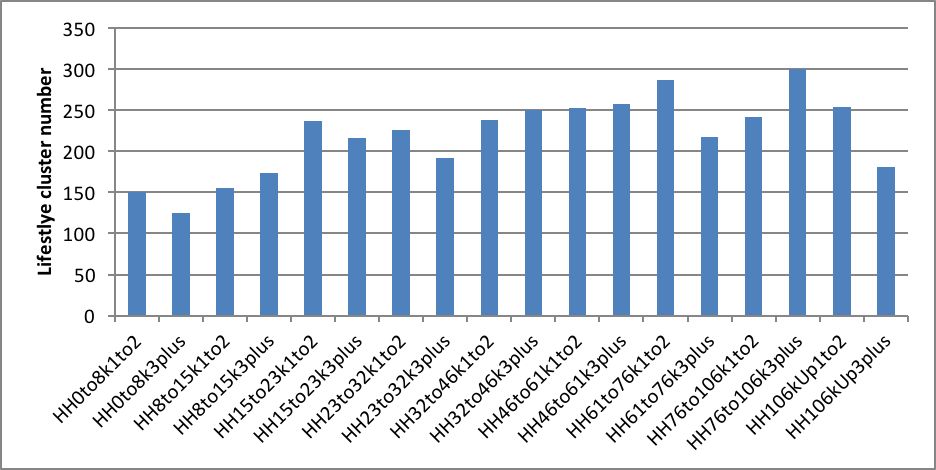
\includegraphics[scale=0.4, trim=0mm 2mm 0mm 0mm]{aa/lifestyle-clusters}
\caption{Lifestyle cluster numbers by Oregon AA household types}\label{fig:aa-lifestyle-clusters}
\end{figure}

\begin{table}     %Table 6-5 Dimensions of Oregon AA household lifestyle
\centering
\caption{Dimensions of Oregon AA household lifestyles}
\label{tab:aa-household-lifestyles}
\begin{tabular}{ccll}
\hline
Dimension & ID & Name & Type of variable \\
\hline
1 & 1 & Space type (6 categories) & Categorical \\
\gray  & 2 & Estimated square feet & Continuous \\
\hline
2 & 3 & Management and business worker's wage & Continuous \\
\gray  & 4 & Professional specialty worker's wage & Continuous \\
  & 5 & Education worker's wage & Continuous \\
\gray  & 6 & Health worker's wage & Continuous \\
  & 7 & Technical worker's wage & Continuous \\
\gray  & 8 & Sales and clerical professional worker's wage & Continuous \\
  & 9 & Sales and service labor worker's wage & Continuous \\
\gray  & 10 & Ag, Forest and Production specialty worker's wage & Continuous \\
  & 11 & Maintenance, construction, repair specialty worker's wage & Continuous \\
\gray  & 12 & Protective and transport specialty worker's wage & Continuous \\
  & 13 & Blue collar labor worker's wage & Continuous \\
\hline
\end{tabular}
\end{table}

\begin{table}     % Table 6-6 Oregon AA household type
\centering
\caption{Oregon AA household types}\label{tab:aa-household-types}
\begin{tabular}{clr}
\hline
Type ID & PECAS Household Type & N \\
\hline
1 & HH0to8k1to2 & 4,132 \\
\gray 2 & HH0to8k3plus & 767 \\
3 & HH8to15k1to2 & 4,031 \\
\gray 4 & HH8to15k3plus & 1,264 \\
5 & HH15to23k1to2 & 5,109 \\
\gray 6 & HH15to23k3plus & 2,089 \\
7 & HH23to32k1to2 & 6,428 \\
\gray 8 & HH23to32k3plus & 3,071 \\
9 & HH32to46k1to2 & 9,874 \\
\gray 10 & HH32to46k3plus & 5,477 \\
11 & HH46to61k1to2 & 8,977 \\
\gray 12 & HH46to61k3plus & 6,150 \\
13 & HH61to76k1to2 & 6,690 \\
\gray 14 & HH61to76k3plus & 5,910 \\
15 & HH76to106k1to2 & 8,166 \\
\gray 16 & HH76to106k3plus & 8,626 \\
17 & HH106kUp1to2 & 8,361 \\
\gray 18 & HH106kUp3plus & 9,610 \\
\hline
\end{tabular}
\end{table}

\subsection{Buying and Selling Allocation Parameters}
Table \ref{tab:bs-allocation-parameters} identifies the estimated parameters of the AA buying and selling allocation module, discussed in \S\ref{sec:aa-pca-technology}. The values of the parameters are discussed in the remainder of this section.

% Table 6-5 AA Buying and Selling Allocation Parameters
\begin{table}
\centering
\caption{Buying and selling allocation parameters}\label{tab:bs-allocation-parameters}
\begin{tabular}{lp{4.8in}c}
\hline
Parameter & Description & Level \\
\hline
$\delta_{size,s}$ & Utility function coefficient for the sensitivity to size & S1 \\
\gray $\delta_{size,b}$ & Utility function coefficient for the sensitivity to size & S1 \\
$\delta_{price,s}$ & Utility function coefficient for the sensitivity to price when selling & S1 \\
\gray $\delta_{price,b}$ & Utility function coefficient for the sensitivity to price when buying & S1 \\
$\delta_{tran,s}$ & Utility function coefficient for the sensitivity to transport utility & S2 \\
\gray $\delta_{tran,b}$ & Utility function coefficient for the sensitivity to transport utility & S2 \\
$\lambda_{s,c}$ & Utility function dispersion parameter for allocation of selling of commodity $c$ & S2 \\
\gray $\lambda_{b,c}$ & Utility function dispersion parameter for allocation of buying of commodity $c$ & S2 \\
$\phi_{s,c,a}$ & Factor adjustment to the composite utility of selling commodity $c$ by activity $a$ & S1/S2 \\
\gray $\phi_{b,c,a}$ & Factor adjustment to the composite utility of buying commodity $c$ by activity $a$ & S1/S2 \\
OptionWeight$_{p,a}$ & Weight of technology option $p$ for activity $a$ & S2 \\
\gray $\kappa_{c,dist}$ & Utility function coefficient for the sensitivity to trip distance when transporting a unit of commodity $c$ & S1 \\
$\kappa_{c,time}$ & Utility function coefficient for the sensitivity to trip travel time when transporting a unit of commodity $c$ & S1 \\
\gray $\kappa_{c,logsum}$ & Utility function coefficient for the sensitivity to trip mode choice composite utility when transporting a unit of commodity $c$ & S1 \\
\hline
\end{tabular}
\end{table}

\subsubsection{Buying and selling allocation parameters}
Buying and selling allocation S2 parameters include the dispersion parameter for allocation of buying and selling commodities ($\lambda_{s,c}, \lambda_{b,c}$), as well as the coefficients for the sensitivity to transport utility ($\delta_{tran,b}, \delta_{tran,s}$). The initial values for these parameters are shown in Table \ref{tab:aa-allocation-commodity}. Also shown is the exchange type assumed in the initial AA runs, which determines the location for the exchange. Floorspace is assumed non-transferable (n), while all other commodities are exchanged in any zone (a). Future runs may restrict non-floorspace exchanges to occur either in the production (p) or consumption (c) zone.

%Table 6-6 AA Buying and Selling Allocation Parameters by Commodity
\begin{table}
\centering
\caption{Buying and selling parameters by commodity}\label{tab:aa-allocation-commodity}
\begin{tabular}{lcccc}
\hline
\multirow{2}{*}{Parameter}& \multicolumn{4}{c}{Commodity categories} \\
\cline{2-5}
& Goods & Services & Labor & Floorspace \\
\hline
\multicolumn{5}{l}{\textit{Buying activity allocation coefficients}} \\
\gray Disperson parameter ($\lambda_{b,c}$) & Calibrated & Calibrated & Calibrated & 5  \\
Size coefficient ($\delta_{size,b}$) & 1 & 1 & 1 & 1 \\
\gray Price coefficient ($\delta_{price,b}$) & -1 & -1 & -1 & -1 \\
Transport coefficient ($\delta_{tran,b}$) & Figure \ref{fig:aa-vot} & Figure \ref{fig:aa-vot} & Figure \ref{fig:aa-vot} & 0  \\
\hline
\multicolumn{5}{l}{\textit{Selling activity allocation coefficients}} \\
\gray Disperson parameter ($\lambda_{s,c}$) & Calibrated & Calibrated & Calibrated & 5  \\
Size coefficient ($\delta_{size,s}$) & 1 & 1 & 1 & 1  \\
\gray Price coefficient ($\delta_{price,s}$) & 1 & 1 & 1 & 1  \\
Transport coefficient ($\delta_{tran,s}$) & Figure \ref{fig:aa-vot} & Figure \ref{fig:aa-vot} & Figure \ref{fig:aa-vot} & 0  \\
\hline
\multicolumn{5}{l}{\textit{Exchange type}} \\
& Mix of $p$ and $a$ & Mix of $p$ and $c$ & C & n  \\
\hline
\end{tabular}
\end{table}

% Labeled as Table 6-7 Value of Time based on Wage Rate and Business Travel share of Trips, but actually a figure
\begin{figure}
\centering

\includegraphics[scale=0.75]{aa/aa-value-of-time}
\caption{Value of time based upon wage rate and business travel share of trips}
\label{fig:aa-vot}
\end{figure}

For residential space, residential buying size terms are also used ($Size_{b,c,k}$ in equation \ref{eq:6.17}). These buying size terms are calculated as the quantity of space type $c$ in zone $k$ divided by the total of all residential space types in zone $k$. (All other buying size terms and selling size terms are left at their default value of 1.0).

Buying and selling composite utility includes allowance for factor and offset adjustments. All factor adjustments, $\phi_{s,c,a}$, are set to 1 and the offset adjustments, $USellRef_{c,a}$ and $UBuyRef_{c,a}$ are set to zero (Table \ref{tab:aa-household-lifestyles}). It is expected that in some cases, as calibration progresses, the factor adjustment may be set to 0 to completely remove the effect of individual buying and selling composite utilities on production utilities and thus on location utilities.

\subsubsection{Time and Cost Weights for Transporting Commodities}
Transport cost coefficients weigh the relative value of time and distance in the transport utility function. The AA transport function includes the overall sensitivity to transport ($\delta_{tran,b}$ and $\delta_{tran,s}$), as well as commodity-specific time and distance coefficients or commodity-specific coefficients on mode-choice logsums. 

The transport coefficient is essentially the inverse of the economic value per trip, allowing the time and distance parameters to be in units of cost per vehicle trip. These costs take into account variations in commodity value (labor or goods) and vehicle occupancy (tons or persons per vehicle). Goods transport costs are incurred at the production end (buying), while services (management and other) and labor transport costs are born at the consumption end (selling) of the exchange. Floorspace is non-transportable, so there are no transport costs (coefficients set to 1 or 0). These parameters are defined in the CommoditiesI.csv AA input file.

Freight commodity time and cost rates were calculated primarily with data from a 2000 WSDOT statewide modeling effort. In many cases, STCC commodity data was converted into the SCTG classification used in AA, weighted by 1999 IMPLAN production data (Make value). These transport costs assume mode/vehicle operating costs and endogenized other cost, wage and mode split components. The transport coefficients are calculated as follows. Figure \ref{fig:aa-vot} shows the relationship assumed to calculate value of time for service-related trips. All monetary values have been converted into 2009 dollars. Note: In some cases final parameter values shown in Table \ref{table_6-10} were modified during calibration and do not follow these formula.

\vspace{10pt}
\noindent For goods:
\begin{itemize}
\item $\delta_{tran,b}$ and $\delta_{tran,s}$ (trip/\$ of goods) = 1/(\$ payload value)
\item $\kappa_{c,time}$ (\$/vehicle-min) = (\$ per veh-hr) / (60min/hr) [user-input]
\item $\kappa_{c,dist}$ (\$/vehicle-mile) =  (\$ per ton-mile) * (Tons per vehicle) [user-input]
\item $\kappa_{c,logsum}$ (\$/mode choice utility) = 0
\end{itemize}

\noindent Which is based on assuming:
\begin{itemize}
\item 100 percent truck mode split [CT output (future)]
\item \$ payload value = \$ per ton*Tons per vehicle
\item \$ per vehicle-hr = \$20.42/Medium truck hour (other modes 0) [user-input]
\item \$ per ton-mile by mode = \$0.12 for MedTruck (\$.04 for Rail, \$3.71 for Air, \$0.01 for 
Barge) [user-input]
\item \$ per ton, ranging from \$18 to 90,691/Ton  (\$7,194/Ton average) 
\item Tons per vehicle: 9 to 22 tons/truck (average 15.6 tons/truck, 51 tons/railcar) [CT 
output (future)]
\end{itemize}

\noindent For labor/services:
\begin{itemize}
\item $\delta_{tran,b}$ and $\delta_{tran,s}$ (trip/\$ of production value) = (Trips per day) / (\$ of production value)

Labor: \$ of production value = (\$Economic wage per hour) * (8 hours/day)

Service: \$ of production value = (\$Annual Industry Use of Commodity) / (Annual vehicle trips) 
\item $\kappa_{c,time}$ = (\$Economic wage per hour)/(60min/hr): only for selected services
\item $\kappa_{c,dist}$ = (\$Operating cost per veh-mile)/(Auto occupancy): only for selected services
\item $\kappa_{c,logsum}$ = 1/\$ out-of-pocket (OPC) cost parameter for associated logsum (PT module 
estimated parameters): for all other services and labor/commute
\end{itemize}

\noindent Which is based on assuming:
\begin{itemize}
\item 100 percent auto mode split
\item Trips per day = 1 for labor commute trips, 1.5 for services (assuming some trip chaining)
\item \$ of production value per trip by purpose (for services) = \$Annual Total Use of 
Commodity/2009 Annual vehicle trips
\item \$ of production value per trip by purpose (for labor) = \$Economic wage per hour = 
(\$ Wage per hour) * (\%BusinessPurposeTrips * 67\% + 33\%)
\item \$ Wage per hour =  2005-2009 ACS PUMS wage data by occupation, where average calculated as annual wages divided by (weeks worked x hrs per week (WKHP)), limited to those working 49+ weeks/yr and not self-employed: \$3.74 to 21.98, average \$16.05 [AA data (future)]
\item \%BusinessPurposeTrips= 2009Modelwide IMPLAN share of total commodity used by industry = Annual IndustryUse/(Annual Household Use+Annual Institution Use]) [AA data (future)]
\item \$Annual Industry, Household, Institution, and Total Use of Commodity = 2009ModelwideIMPLAN data by trip purpose [AA data (future)]
\item 2009 Annual vehicle trips = 1994-1996 Oregon Travel Behavior Survey trips per HH by 
trip purpose * 2009 modelwide households
\item Auto Occupancy = 1994-1996 Oregon Travel Behavior Survey by trip purpose: 1.2 to 2.3, 
average 1.5 [user-input]
\item \$Operating cost per veh-mile = \$0.148/mile, consistent with PT module [user-input]
\end{itemize}

\subsubsection{Buying and selling price sensitivity coefficients}

The coefficients for the sensitivity to price when buying or selling ($\delta_{price,s}, \delta_{price,b}$), found in the buying and selling allocation utility functions, are set to 1 for all commodities, positive when selling and negative when buying. These are shown in Table \ref{table_6-8}. Thus, the utility function is in units of equivalent 2009 dollars.

% The transport coefficients table (Table 6-8 in original manuscript) is too large to fit in either landscape or portrait
% mode, even with footnote size text. So put in a placeholder for it, and we'll manually insert the oversized page in the
% final version of this document.
\begin{table}   % Placeholder
\centering
\caption{AA transport coefficients (per unit of production)}
\label{tab:aa-transport-coefficients}

\includegraphics[scale=0.5]{graphics/placeholder-female-superhero-c}
\end{table}
\begin{table*}
\centering

\includegraphics[scale=0.5]{graphics/placeholder-male-superhero-c}
\end{table*}

\subsection{Imports and Exports Model Parameters}
Table \ref{tab:aa-classic-parameters} identifies the estimated parameters of the classic style AA imports and exports model including floorspace imports, discussed in \S\ref{sec:aa-import-export} and \S\ref{sec:aa-floorspace-imports}. The values of the parameters are discussed in the remainder of this section.

% This combines what used to Tables 6-9 and 6-10, which appear to have the same header. Moreover, the latter was
% never referenced, so rather than lose the info it contained I simply put into bottom of this table.
\begin{table}
\centering
\caption{Classic-style AA imports and exports model parameters}
\label{tab:aa-classic-parameters}
\begin{tabular}{lL{4.9in}c}
\hline
Parameter & Description & Level \\
\hline 
$PriceRef_{c,i}$ & Reference price per unit for import of commodity $c$ & S1 \\
\gray $PriceRef_{c,e}$ & Reference price per unit for export of commodity $c$ & S1 \\
$QRef_{c,i}$ & Quantity of commodity $c$ imported to exchange location when the unit exchange price for commodity $c$ in exchange zone $k$ is at its import reference level $PriceRef_{c,i}$ & S1 \\
\gray $QRef_{c,e}$ & Quantity of commodity $c$ exported from exchange location when the unit exchange price for commodity $c$ in exchange zone $k$ is at its export reference level $PriceRef_{c,e}$ & S1 \\
$\gamma_{c,I}$ & Function coefficient for the rate of increase in imports of commodity $c$ for slope term & S1 \\
\gray $\gamma_{c,e}$ & Function coefficient for the rate of increase in exports of commodity $c$ for slope term & S1 \\
$\mu_{c,I}$ & Function coefficient for the rate of increase in imports of commodity $c$ for linear term & S1 \\
\gray $\mu_{c,e}$ & Function coefficient for the rate of increase in exports of commodity $c$ for linear term & S1 \\
$\eta_{c,I}$ & Function coefficient for sensitivity to difference in exchange price for commodity $c$ concerning increase in imports of commodity $c$ for exponent term & S1 \\
\gray $\eta_{c,e}$ & Function coefficient for sensitivity to difference in exchange price for commodity $c$ concerning increase in exports of commodity $c$ for exponent term & S1 \\
\hline
$F0Price$ & Reference price per unit of floorspace & S2 \\
\gray $PMidpoint$ & Quantity of floorspace supplied when the unit exchange price for floorspace in exchange zone $k$ is at its reference level $F0Price$ & S2 \\
$FDelta$ & Function coefficient for the rate of increase in imports of floorspace for slope term & S1 \\
\gray $FSlope$ & Function coefficient for the rate of increase in imports of floorspace for linear term & S2 \\
$FEta$ & Function coefficient for sensitivity to difference in exchange price for floorspace concerning the increase in floorspace supply for exponent term & S2 \\
\hline
\end{tabular}
\end{table}

In previous versions of the model, these parameters were critically important as they represented the appearance of imports and exports in the region. These import and export functions have been largely replaced by an explicit treatment of the flow of imports and exports to and from world-market zones to internal zones. The parameters in this table are now given appropriately small values to allow small amounts of imports to appear (and exports to disappear) in individual zones in cases where small imports or exports are necessary to balance supply and demand but quantities are irrelevant for transportation planning purposes.

% Table 6-10, AA Classic Style Imports and Exports Model Parameters, is apparently never referenced, so omitted

Table \ref{aa-floorspace-import-parameters} shows the floorspace import functions. Floorspace import functions represent the supply of the physical inventory of floorspace by landlords. These parameters were calibrated through an investigation of observed prices and vacancy rates, as landlords tend to let more space go vacant as prices decline.

\subsubsection{Import and export function parameters}
Import and export reference price per unit of import of each commodity $c$ ($PriceRef_{c,i}$, $PriceRef_{c,e}$) are currently set to 1.0, so AA thus operates in terms of relative prices with respect to the 2009 IMPLAN base year prices. The reference quantity represents the magnitude of imports and exports that are acceptable outside of the explicit treatment in the world market zones. These are currently set to 1 million, and could be reduced further as the model is improved through further calibration. 

The remaining coefficients regulate the response of this import/export quantity in any zone to price changes. These parameters include a linear term ($\mu_{c,i}, \mu_{c,e}$), exponent slope term ($\gamma_{c,i}, \gamma_{c,e}$) and a coefficient for the sensitivity to exchange zone price differences ($\eta_{c,i}, \eta_{c,e}$). The impact of these terms on the reference quantity and price can be seen graphically in Figure \ref{fig:aa-import-parameters}.

\begin{figure}      % Originally Figure 6.5 - still needs considerable cleanup
\centering
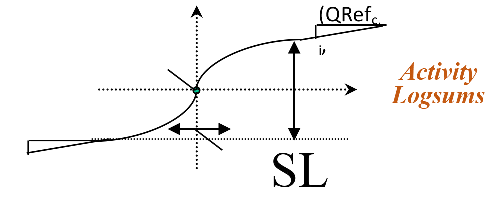
\includegraphics[scale=0.8]{aa/errant_figure_6_5}
\caption{Import function parameters}\label{fig:aa-import-parameters}
\end{figure}

The slope terms were set at 10 percent of the reference quantities (negative export slope) and the exponent at 20 percent, except for floorspace, as shown in Table \ref{tab:aa-ie-function-parameters}.

\begin{table}   % Table 6-11 AA Import/Export Function Parameters
\centering
\caption{AA import-export function parameters}\label{tab:aa-ie-function-parameters}
\begin{tabular}{lccccc|ccccc}
\hline
Commodity & \multicolumn{5}{c|}{Import coefficients} & \multicolumn{5}{c}{Export coefficients} \\
\cline{2-11}
categories & $QRef_{c,i}$ & ~$\gamma_{c,i}$~ & ~$\eta_{c,i}$~ & ~$\mu_{c,i}$~ & $PriceRef_{c,i}$ & $QRef_{c,e}$ & $~\gamma_{c,e}$~ & ~$\eta_{c,e}$~ & ~$\mu_{c,e}$~ & $PriceRef_{c,e}$ \\
\hline
All & 1e6 & 0.2 & 1e6 & 1e6 & 1 & 1e6 & 0.2 & -1e6 & -1e6 & 1 \\
\hline
\multicolumn{11}{l}{\footnotesize Note: $PriceRef$ values are S1 parameters (see \S\ref{sec:ned-s1-s2}) from AA input file ExchangeImportExportsI.csv}
\end{tabular}
\end{table}

\subsubsection{Import and export function parameters}
The bulk of import and exports are represented explicitly in the six world markets. Thus goods and services must travel along the highway network to reach the import/export exchange location, representing the costs of transporting these physical goods to the external markets. For more discussion of these world markets and associated assumptions see Sections \ref{sec:model-area-geography} (page \pageref{sec:model-area-geography}) and \ref{sec:category-definitions} (page \pageref{sec:category-definitions}).

These imports are ``made'' by the importing activities, while the exports are ``used'' by the exporting activities.  The quantity of these activities is developed in the aggregate economic flows table, and by the NED module for future years as part of the overall balancing of the economy. In the base year the activity constraint procedure is used to establish the constants ($Constant_{a,z}$, equation \ref{eq:6.02}) that are required to draw the imports and exports from and to the correct direction into and out of the model region. These constants are applied in future years so that the directionality tends to be maintained but can respond to transportation conditions.  

There is overall elasticity in these imports and exports, this elasticity was adjusted through the 
calibration of the $\lambda_{m,a}$ parameter for the importing and exporting activities.  

\subsubsection{Floorspace import parameters}

Each floorspace type has a supply function in a specific land use zone. The shape of the supply function is specified with parameters that are documented in this section, and the size (magnitude) of the supply function is scaled based on the inventory of the space in that zone.

FloorspaceSupplyI.csv file is described immediately below:
\begin{itemize}
\item $ZoneNumber$ is an integer value of land use zone (LUZ) that is the exchange location zone; a value of -1 indicates all land use zones not considered explicitly in other rows using single zone numbers in single rows for the commodity
\item $Commodity$ are text characters of name of commodity; this must match exactly the commodity name used in CommoditiesI;
\item $SupplyFunctionMidpointFactor$ is the real value of import function quantity of commodity imported to exchange location when the unit exchange price for commodity in exchange zone is at its import reference level $PriceIRef_c$; this is $QiRefc$ in equation 21 in the Theoretical Formulation document;
\item $SupplyFunctionMidpointPrice$ is the real value of import function reference price per unit for import of commodity; this is $PriceIRefc$ in equations 21 and 23 in the Theoretical Formulation document;
\item $SupplyFunctionEta$ is the real value of import function coefficient for sensitivity to difference in exchange price for commodity concerning increase in imports of commodity for exponent term; this is $\eta_{ic}$ in equation 23 in the Theoretical Formulation document;
\item $SupplyFunctionDeltaFactor$ is a real value of import function coefficient for the rate of increase in imports of commodity for exponent term; this is $\Delta_{ic}$ in equation 21 in the Theoretical Formulation document;
\item $SupplyFunctionSlopeFactor$ is the real value of import function coefficient for the rate of increase in imports of commodity for linear term; this is $\mu_{ic}$ in equation 21 in the Theoretical Formulation document;
\item $NoQuantityPrice$ is a real value of export reference price per unit for export of commodity; this is $PriceERefc$ in equations 22 and 24 in the Theoretical Formulation document;
\item $NoQuantitySlope$ is a real value of export function coefficient for the rate of increase in exports of commodity for linear term; this is $\mu_{ec}$ in equation 22 in the Theoretical Formulation document;
\item $MonitorExchange$ are text characters indicating whether interim values for the commodity in the exchange zone are to be written to the log file in order to monitor the AA Module solution algorithm; ``true'' indicates the interim values are to be written, ``false'' indicates the interim values are not to be written
\end{itemize}
\noindent For Oregon model ZoneNumber for each floorspace type is set to -1 and MonitorExchange is set to ``false'' for all of the floorspace types. The calibrated values are shown in Table \ref{aa-floorspace-import-parameters}.

\begin{sidewaystable}   % Table 6-12 AA Floorspace Import Parameters
\centering
\caption{AA floorspace import parameters}\label{aa-floorspace-import-parameters}
%\small
\begin{tabular}{lC{0.6in}C{0.6in}C{0.6in}C{0.6in}C{0.6in}C{0.6in}C{0.6in}}
\hline
Commodity & Supply function midpoint factor & Supply function midpoint price & Supply
function eta & Supply function delta factor & Supply function slope factor & No quantity price & No quantity slope \\
\hline
FLR Accommodation & 0.28 & 5 & 0.44 & 0.67 & 0.0008 & 5 & -1.3E-05 \\
\gray FLR Agriculture & 0.28 & 0.03 & 60 & 0.67 & 0.533 & 0.023 & -0.0222 \\
FLR Government Support & 0.28 & 5 & 0.55 & 0.67 & 0.00123 & 6.5 & -1.3E-05 \\
\gray FLR K12 & 0.28 & 5 & 0.55 & 0.67 & 0.0008 & 7 & -1.3E-05 \\
FLR Heavy Industry & 0.28 & 3.5 & 0.629 & 0.67 & 0.00114 & 7 & -1.3E-05 \\
\gray FLR Hospital & 0.28 & 5 & 0.55 & 0.67 & 0.0008 & 10 & -1.3E-05 \\
FLR Institutional & 0.28 & 5 & 0.55 & 0.67 & 0.0008 & 10 & -1.3E-05 \\
\gray FLR Light Industry & 0.28 & 3.5 & 0.629 & 0.67 & 0.00114 & 7 & -1.3E-05 \\
FLR Logging & 0.28 & 0.03 & 60 & 0.67 & 0.533 & 0.025 & -0.0889 \\
\gray FLR Office & 0.28 & 5 & 0.55 & 0.67 & 0.00123 & 7 & -1.3E-05 \\
FLR Retail & 0.28 & 5 & 0.44 & 0.67 & 0.000667 & 10 & -1.3E-05 \\
\gray FLR Warehouse & 0.28 & 3.5 & 0.629 & 0.67 & 0.00178 & 4.5 & -1.3E-05 \\
FLR MH & 0.056 & 0.15 & 1.1 & 0.804 & 0.01 & 6 & -3.3E-05 \\
\gray FLR MF & 0.056 & 0.15 & 1.1 & 0.804 & 0.01 & 6 & -3.3E-05 \\
FLR AT & 0.056 & 0.15 & 1.1 & 0.804 & 0.01 & 6 & -3.3E-05 \\
\gray FLR SFD & 0.056 & 0.15 & 1.1 & 0.804 & 0.01 & 6 & -3.3E-05 \\
FLR RRMH & 0.056 & 0.15 & 1.1 & 0.804 & 0.01 & 6 & -3.3E-05 \\
\gray FLR RRSFD & 0.056 & 0.15 & 1.1 & 0.804 & 0.01 & 6 & -3.3E-05 \\
\hline
\end{tabular}
\end{sidewaystable}

\section{Inputs and Outputs}\label{sec:aa-inputs-outputs}
The inputs and output of the AA module are listed in Tables \ref{tab:aa-inputs} and \ref{tab:aa-outputs}, respectively. The remainder of this section discusses them in more detail, including selected AA inputs and processing to generate base year input data.

\begin{sidewaystable}
\centering
\caption{AA module inputs}\label{tab:aa-inputs}
\begin{tabular}{L{4.5in}L{2.75in}L{1.1in}}
\hline
Data element & File(s) & Source \\
\hline

Modelwide total production quantity of activity $a$ ($TW_a$), modified by AA p-processor & ActivityTotalsI.csv, ActivityTotalsW.csv & NED (industry \$), SPG1 (HHs) \\

\gray Total production quantity of activity by alpha zone in the 2009 base year ($TW_{a,z}$), used to set zonal constants in constrainted AA run & ActivityConstraintsI.csv & Exogenous \\

Quantities of total floorspace inventory by alpha zone & FloorspaceI.csv & ALD \\

\gray Increments of total floorspace change in past year by alpha zone & Increments.csv & ALD \\

Fixed constant-production rate agricultural and forest lands by zone & AgForestFloorspace.csv (used only in AA, adds FloorspaceI.csv resource land sqft) & Exogenous \\

\gray Mode choice composite utility for commodity $c$ between beta zones $k$ and $z$ ($MSLogSum_{c,k,z}$) & **mcls\_beta.zmx & PT \\

Auto and commercial vehicle times and distances traveled by commodity $c$ between beta zones $k$ and $z$ ($Time_{c,k,z}$, $Dist_{c,k,z}$) & betapk***dist.zip, betapk***time.zip, worldZoneDistances.csv & VISUM \\

\gray Proportion of modelwide quantity of production activity $a$ in zone $z$ in the prior year ($PrevW_{a,z}$) & ActivityLocations.csv & Prev year AA \\

Unit prices for commodities by beta zones ($Price_{c,k}$) & ExchangeResults.csv (prior), ExchangeResultsI.csv (current) & Prev year AA \\

\gray Production size terms by zone $z$ and activity $a$ ($Size_{a,z}$) & ActivitySizeTermsI.csv & Exogenous \\

Aggregate activities definitions/parameters & ActivitiesI.csv & Exogenous \\

\gray Commodity definitions/parameters and transportation-based cost coefficients & CommoditiesI.csv & Exogenous \\

Floorspace constants & FloorspaceSupplyI.csv & Exogenous \\

\gray Industry technology options and related commodity make and use coefficients & TechnologyOptionsI.csv & Exogenous \\

Import/export function coefficients by beta zone & ExchangeImportExportI.csv & Exogenous \\

\gray List of alpha zones and beta zones & alpha2beta.csv, processed into FloorspaceZonesI.csv and PECASZonesI.csv & Exogenous \\

Index numbers used to identify activities and commodities in ZonalMakeUse.csv (only if stringsInZonalMakeUse is set to false in properties file) & ActivityNumbers.csv, CommodityNumbers.csv & Exogenous \\

\gray Trip length/time distribution input (optional) & HistogramsI.csv & Exogenous \\
\hline
\end{tabular}
\end{sidewaystable}   % Table 6-13 AA Inputs
\begin{sidewaystable}
\centering
\caption{AA module outputs}\label{tab:aa-outputs}
\begin{tabular}{L{4.25in}L{2.5in}L{1.5in}}
\hline
Data element & File(s) & User(s) \\
\hline
AA Working files (see above) & & AA \\
\gray Internal commodity dollar flows (goods, services, labor) between beta zones & buying\_commodity.zipMatrix, selling\_commodity.zipMatrix & PT (selling labor), CT (goods) \\

Labor dollar production by occupation and household category and consumption by occupation and industry expanded to alpha zones & TAZDetailedMake.csv, TAZDetailedUse.csv & SPG2 (production) \\

\gray Labor dollar production and consumption by occupation category expanded to alpha zones & laborDollarProductionSum.csv, laborDollarConsumptionSum.csv, FloorspaceZoneTotalMakeUse.csv & PT \\

Activity quantities and composite utilities for beta and alpha zones & ActivityLocations.csv, ActivityLocations2.csv & SPG2 (alpha), Next yr AA (beta) \\

\gray Occupied quantities and unit prices for floorspace in beta zones & ExchangeResults.csv & Next yr ALD \\

Import/export quantities of commodities (\$ flows) to beta zones & ExchangeResults.csv & CT diagnostics \\

\gray Commodity quantities make and use by alpha zone & FloorspaceZoneTotalMakeUse.csv, FloorspaceZoneTotalMakeUse.bin & CT (future) \\

Modelwide composite utilities of production by activity & ActivitySummary.csv & Next yr NED (future) \\

\gray Solved beta zone industry-commodity production and consumption technical coefficients & ZonalMakeUse.csv & Diagnostics \\

Commodity beta zone composite utilities & CommodityZUtilities.csv & Diagnostics \\

\gray Trip length distribution histogram output & Histograms.csv & Diagnostics \\

Summary totals from ZonalMakeUse.csv & MakeUse.csv & CT, diagnostics \\

\gray Summary totals from ExchangeResults.csv & ExchangeResultsTotals.csv & Diagnostics \\

Outcome of technology choice by each activity in each beta zone & TechnologyChoice.csv & Diagnostics \\

\gray Amount of flow that is intrazonal & PctIntrazonalxCommodityxBzone.csv & Diagnostics, calibration of short trips \\

Relative importance of commodity random utility error term for each activity, for buying & ProductionErrorTermSizes.csv & Diagnostics, advanced calibration \\

\gray Relative importance of commodity random utility error term for each activity, for selling & ProductionErrorTermSizes.csv & Diagnostics, advanced calibration \\
\hline
\end{tabular}
\end{sidewaystable}   % Table 6-14 AA Outputs 

AA produces the following working files pulling data from other modules, as listed above and 
discussed with the AA p-processor in \S\ref{sec:aa-p-processor}:
\begin{itemize}
\item {[ActivityTotalsW.csv] from [ActivityTotalsI.csv], [activity\_forecast.csv], [householdsByHHCategory.csv], [trade\_forecast.csv], [government\_forecast] and [TechnologyOptionsI.csv]}
\item {[FloorspaceW.csv] from [AgForestFloorspace.csv] and [FloorspaceI.csv]}
\item {[ActivitiesZonalValuesW.csv] from [ActivitiesZonalValuesI.csv], [Increments.csv] and [ActivityLocations.csv]}
\item {[TechnologyOptionsW.csv] from [TechnologyOptionsI.csv]}
\end{itemize}

\noindent A few notes on AA files:
\begin{itemize}
\item When AA looks for previous year prices, it first looks for ExchangeResultsI.csv in the current year 
directory and if not found, ExchangeResults.csv output from the previous year is used.
\item AA has an option to produce trip length/time histograms on request. To do so, the HistogramsI.csv input file must be specified with the following column fields: commodity name, skim (distance/time matrix), the upper bound of up to 100 trip length or time bands (typically miles/minutes). All commodities must have the same number of bands in the file, with zeros listed for any bands not used. Each listed commodity generates an output Histograms.csvfile with buying/selling quantity (commodity dollar value) that falls within each band, as well as the average trip length/time value of each band. One more band than the number of upper bounds, as the last band is values exceeding the upper-most band.
\end{itemize}

\subsection{Modelwide Activity by Category}
Each period, AA allocates modelwide production activity, $TW_a$ output from the NED module, among beta zones. The previous period's allocation by zone, $PrevWa,z$, influences the outcome of the current year. The number of households by income and household size categories is used as the measure of residential activity and as a size term, in the allocation of labor ($Sizea,z$) and the location of construction activity. Industry and government as well as import/export activity come from the NED module (activity\_forecast.csv, government\_forecast.csv, trade\_forecast.csv), while household counts come from the SPG1 module (householdsByHHCategory.csv). The AA pre-processor augments the NED industry output by adding office-based activity by industry.

Base year modelwide industry production (margined make) by activity in 2009 dollars used for $TW_a$ comes from 2009 IMPLAN data (with some adjustments to add office activity and adjust education activity dollars), also processed as part of the Make and Use Technical coefficients as discussed in \S\ref{sec:pa-allocation-parameters}. Base year modelwide household counts used as activity totals in AA are obtained from SPG1 module output. In the base year, SPG1 is constrained by the NED 2009 employment forecasts that are consistent with the 2009 IMPLAN industry activity data. 

Each year AA adds to these NED and SPG values by calculating the following (resulting in AA input file, ActivityTotalsI.csv):
\begin{itemize}
\item Modelwide amount of potential imports and exports based on the total internal use and total internal make in the previous year.  
\item Modelwide amount of office support activities based on the use of office support by the production activities.
\end{itemize}
\noindent The base year modelwide values are shown in Tables \ref{tab:aa-industry-production} through \ref{tab:aa-imports-exports}.

%Table 6-15 2009 Modelwideproduction by each activity in 2009 dollars
\begin{sidewaystable}
\centering
\caption{Modelwide industry production by activity, in 2009 dollars}
\label{tab:aa-industry-production}
\small
\begin{tabular}{lrr|lrr}
\hline
Activity - Industry & Total amount in 2009 & 2009 employees & Activity - Industry & Total amount in 2009 & 2009 employees \\
\hline
RES\_agmin\_ag & 16,903,898,303 & 102,010 & TRNS\_trns\_off & 2,125,367,253 & 45,390 \\
\gray RES\_forst\_log & 2,519,144,897 & 8,212 & INFO\_info\_off\_li & 15,239,006,202 & 6,691 \\
RES\_offc\_off & 1,332,074,223 & 58,746 & INFO\_info\_off & 2,881,870,409 & 49,465 \\
\gray ENGY\_elec\_hi & 8,621,276,855 & 6,642 & UTL\_othr\_off\_li & 8,378,148,941 & 18,973 \\
ENGY\_ngas\_hi & 3,603,145,996 & 696 & UTL\_othr\_off & 1,114,027,683 & 11,593 \\
\gray ENGY\_ptrl\_hi & 4,631,318,359 & 1,760 & FIRE\_fnin\_off & 31,902,799,194 & 150,467 \\
ENGY\_offc\_off & 1,912,330,649 & 9,839 & FIRE\_real\_off & 15,446,998,046 & 139,527 \\
\gray CNST\_main\_xxx & 3,690,346,435 & 22,722 & HLTH\_hosp\_hosp & 12,295,007,812 & 88,868 \\
CNST\_nres\_xxx & 6,542,617,309 & 60,252 & HLTH\_care\_inst & 3,849,533,203 & 68,309 \\
\gray CNST\_othr\_xxx & 8,729,001,953 & 32,922 & HLTH\_othr\_off\_li & 18,144,155,090 & 130,909 \\
CNST\_res\_xxx & 6,740,919,189 & 44,474 & K12\_k12\_k12 & 12,626,084,053 & 171,266 \\
\gray CNST\_offc\_off & 2,666,187,151 & 53,353 & K12\_k12\_off & 2,777,603,399 & 55,024 \\
MFG\_food\_hi & 10,829,728,776 & 23,936 & HIED\_hied\_off\_inst & 4,569,757,377 & 79,243 \\
\gray MFG\_food\_li & 10,829,728,776 & 15,123 & ENT\_ent\_ret & 3,571,715,370 & 79,205 \\
MFG\_htec\_hi & 13,063,887,807 & 9,623 & HOSP\_acc\_acc & 3,539,955,230 & 35,959 \\
\gray MFG\_htec\_li & 13,063,887,807 & 5,323 & HOSP\_eat\_ret\_acc & 12,374,280,273 & 219,249 \\
MFG\_hvtw\_hi & 14,441,531,006 & 40,903 & SERV\_tech\_off & 22,817,588,607 & 219,409 \\
\gray MFG\_hvtw\_li & 14,441,531,006 & 35,469 & SERV\_site\_li & 5,828,886,779 & 57,739 \\
MFG\_lvtw\_hi & 12,978,764,067 & 18,393 & SERV\_home\_xxx & 456,867,797 & 54,769 \\
\gray MFG\_wdppr\_hi & 11,847,955,596 & 34,188 & SERV\_bus\_off & 14,387,504,547 & 172,891 \\
MFG\_offc\_off & 10,165,454,716 & 115,552 & SERV\_nonp\_off\_inst & 9,376,816,406 & 133,060 \\
\gray WHSL\_whsl\_ware & 19,829,592,529 & 111,388 & SERV\_stor\_ret & 5,164,732,788 & 80,744 \\
WHSL\_offc\_off & 1,733,860,878 & 23,800 & GOV\_admn\_gov & 19,036,836,853 & 80,323 \\
\gray RET\_auto\_ret & 7,439,574,272 & 99,409 & GOV\_offc\_off & 10,008,657,941 & 184,378 \\
RET\_stor\_ret & 16,026,845,092 & 254,174 & FGOV\_acct\_gov & 93,817,953,918 & 0 \\
\gray RET\_stor\_off & 1,518,361,266 & 31,948 & SLGOV\_acct\_gov & 71,879,103,322 & 0 \\
RET\_nstor\_off & 2,193,797,363 & 44,300 & CAP\_acct\_gov & 69,549,704,567 & 0 \\
\gray TRNS\_trns\_ware & 14,723,200,435 & 66,561 &  &  &  \\
\hline
\end{tabular}
\end{sidewaystable}


\begin{table}   % Formerly Table 6-16
\centering
\caption{Modelwide household production by activity, in 2009 dollars}\label{tab:production-activity}
\begin{tabular}{lr|lr}
\hline
Activity--Households & Total 2011 amount & Activity--Households & Total 2011 amount \\
\hline
HH0to8k1to2 & 114,469 & HH32to46k3plus & 126,609 \\
\gray HH0to8k3plus & 23,154 & HH46to61k1to2 & 196,680 \\
HH8to15k1to2 & 166,181 & HH46to61k3plus & 136,043 \\
\gray HH8to15k3plus & 37,181 & HH61to76k1to2 & 133,215 \\
HH15to23k1to2 & 179,197 & HH61to76k3plus & 120,596 \\
\gray HH15to23k3plus & 59,952 & HH76to106k1to2 & 154,108 \\
HH23to32k1to2 & 187,491 & HH76to106k3plus & 170,804 \\
\gray HH23to32k3plus & 80,364 & HH106kUp1to2 & 153,655 \\
HH32to46k1to2 & 240,622 & HH106kUp3plus & 176,127 \\
\hline
\end{tabular}
\end{table}

%Table 6-17 Modelwide import and exports for each commodity in 2009 dollars
\begin{sidewaystable}
\centering
\caption{Modelwide imports and exports for each commodity, in 2009 dollars}
\label{tab:aa-imports-exports}
\small
\begin{tabular}{lrr|lrr}
\hline
Activity & Imports & Exports & Activity & Imports & Exports \\
\hline
sctg01\_fkp\_lvsk & 260,851,452 & 402,771,058 & sctg30\_oth\_clth & 3,501,242,543 & 517,835,114 \\
\gray sctg02\_fkp\_agri\_cereal & 591,333,272 & 485,384,922 & sctg31\_cms\_min & 1,356,212,151 & 877,088,616 \\
sctg03\_fkp\_agri\_other & 1,099,383,757 & 6,652,824,240 & sctg32\_mit\_metl\_base & 3,520,421,862 & 3,018,300,425 \\
\gray sctg04\_fkp\_feed & 763,912,960 & 157,695,428 & sctg33\_mit\_metl\_prod & 2,704,359,252 & 2,533,120,109 \\
sctg05\_fkp\_food\_meat & 2,921,116,467 & 2,043,552,639 & sctg34\_mit\_mach & 7,315,651,539 & 4,377,044,071 \\
\gray sctg06\_fkp\_agri\_grain & 855,005,202 & 761,763,359 & sctg35\_mit\_elct & 11,314,880,451 & 21,885,691,855 \\
sctg07\_fkp\_food\_prep & 5,311,390,317 & 9,382,925,853 & sctg36\_mit\_tran & 6,976,890,863 & 3,168,379,696 \\
\gray sctg08\_fkp\_food\_alc & 1,431,454,151 & 1,156,635,454 & sctg37\_mit\_inst\_transp & 2,147,223,976 & 2,603,475,287 \\
sctg10\_cms\_clay & 73,318,169 & 95,534,556 & sctg38\_mit\_inst\_prec & 3,143,044,038 & 2,301,165,169 \\
\gray sctg11\_cms\_sand & 17,333,501 & 163,311,587 & sctg39\_oth\_furn & 1,872,685,394 & 1,103,630,305 \\
sctg13\_cms\_mine\_nonmet~~~~~~~~~~ & 144,903,688 & 34,035,256 & sctg40\_oth\_misc & 4,774,667,512 & 1,856,532,608 \\
\gray sctg14\_cms\_mine\_met & 507,173,011 & 1,315,595,424 & sctg41\_waste\_scrap & 470,266,803 & 514,256,780 \\
sctg15\_pcc\_coal & 717,887,113 & 34,023,971 & higher\_education & 832,993,534 &  \\
\gray sctg16\_pcc\_petr\_crude & 1,590,154,115 & 242,077,538 & energy & 1,143,833,082 & 3,123,152,392 \\
sctg17\_pcc\_fuel & 5,642,668,465 & 21,714,405 & retail\_trade & 1,961,754,163 & 3,929,056,354 \\
\gray sctg18\_pcc\_petr\_oil & 2,821,334,232 & 10,857,202 & transport & 3,101,392,984 & 3,152,134,411 \\
sctg19\_pcc\_coal\_prod & 4,069,050,714 & 200,319,354 & wholesale\_trade & 2,033,744,399 & 3,135,668,823 \\
\gray sctg20\_pcc\_chem\_basic & 1,891,511,255 & 1,126,536,613 & construction & 12,590,735,942 & 9,180,101,387 \\
sctg21\_pcc\_chem\_pharma & 6,235,158,377 & 764,919,598 & communications\_and\_utilities & 7,869,734,616 & 5,678,834,996 \\
\gray sctg22\_pcc\_chem\_fert & 404,925,018 & 179,061,241 & accommodations & 2,541,892,752 & 3,270,897,187 \\
sctg23\_pcc\_chem\_prod & 3,300,069,335 & 994,754,044 & personal\_and\_other\_services\_and\_amusements & 1,871,340,674 & 4,882,028,098 \\
\gray sctg24\_pcc\_petr\_plast & 4,398,887,943 & 2,051,431,134 & entertainment\_services & 1,089,285,393 & 407,917,914 \\
sctg25\_fwp\_logs & 340,809,605 & 1,101,015,179 & food\_services & 333,886,154 & 720,016,802 \\
\gray sctg26\_fwp\_wood & 651,283,882 & 4,716,264,380 & health\_services & 1,230,526,561 & 928,962,118 \\
sctg27\_ppp\_papr\_puplp & 840,672,962 & 4,508,321,602 & fire\_business\_and\_professional\_services & 30,845,752,639 & 6,322,315,673 \\
\gray sctg28\_ppp\_papr\_paper & 1,240,237,671 & 757,806,729 & government\_administration & 3,567,099,663 & 8,268,890,580 \\
sctg29\_ppp\_papr\_print & 1,703,591,533 & 913,103,214 & education\_reports\_to\_sponsors & 37,468,124 & 3,594,244,993 \\
\hline
\end{tabular}
\end{sidewaystable}

\subsection{Floorspace Quantities by Category by Zone}\label{sec:aa-floorspace-quantities}
Floorspace is an important AA input. It establishes the available exchange locations for production activities. It is received as a fixed amount of space, from the ALD module. For the base year, floorspace quantities by industry and zone (alpha zone, aggregated to beta zones for use in AA) were generated synthetically for ALD. The development of the base year floorspace estimate is discussed in \S\ref{sec:ald-baseyear-floorspace} (page \pageref{sec:ald-baseyear-floorspace}).

In AA agriculture and logging resource lands are treated slightly differently than in ALD. AA requires a consistent use of floorspace per employee per year in a given industry. Resource lands are also less available in urban areas. A base year estimate of the resource lands was developed based on zoning coverage and used as a constraint on allocation of base year employees using these resource lands (see \S\ref{sec:ald-baseyear-floorspace} and \S\ref{sec:aa-zonal-activity-targets}). Selected locations in the halo counties and outside of Oregon UGBs were allowed to exceed the zoning restriction. In both, agriculture and forestry production activities, a single acre per employee usage rate was assumed for each industry employee. This is a simplification of prior PI-based assumptions of 9.1 and 50.1 acres/employee for ag/mining and forestry/logging, respectively (representing the most intensive acres per agriculture employee of the modeled counties).  

The result is a base year amount of land available to AA (AgForFloorspace.csv). These lands (quantity and location) are assumed to be fixed for the duration of the model. In the future, a more sophisticated submodel could be built to address the different land use intensities of agriculture and timberlands, urban-rural conversion of lands, as well as annually rotate timber harvests to un-cut timberland.

\subsection{Road Network Travel Conditions}
AA location decisions are influenced by transport costs and times to obtain factor inputs and reach markets. In addition the composite utility of personal travel across all modes is used in AA, calculated for the previous year in the PT module. 

AM peak period (7-9 AM) auto travel times and costs (both outbound and return) are used for goods and selected service commodities. Identification of the imports/exports of goods commodities requires the multimodal networks used for network assignment to include travel conditions to/from the world market zones (6000 zones). Commercial vehicle skims will be used for selected goods commodities when they become available, allowing industry response to weight restrictions (i.e., increased heavy truck transport costs influence industry location decisions). PT-generated peak mode choice composite utility values,based on time and cost across all modes of travel, are used to represent the travel conditions for labor flows and selected personal services. The assumed travel skims are listed in Table \ref{tab:assumed-network-conditions} for all commodities (AA input CommoditiesI.csv).

These PT outputs are in a compressed OD matrix format, ``squeezed'' from alpha to beta zones for use in the AA module. Initial values were provided by loading the model networks used in the highway and transit network assignment modules. The base year employs preliminary output developed from metro area data. 

% Table 6-18 Assumed Network Travel Conditions by Commodity
\begin{table}
\centering
\caption{Assumed network travel conditions by commodity}
\label{tab:assumed-network-conditions}
\small
\begin{tabular}{ll}
\hline
Commodity & Travel skim(s) \\
\hline
\rowcolor{orange!20}\multicolumn{2}{l}{\textit{Goods commodities}} \\
All SCTG goods commodities & betapktrk1time, betapktrk1dist, betapktrk1toll \\
\rowcolor{orange!20}\multicolumn{2}{l}{\textit{Occupation Labor Commodities}} \\
A1-Mgmt Bus & w7mcls\_beta \\
\gray B1-Prof Specialty & w7mcls\_beta \\
B2-Education & w4mcls\_beta \\
\gray B3-Health & w7mcls\_beta \\
B4-Technical Unskilled & w1mcls\_beta \\
\gray C1-Sales Clerical Professionals & w4mcls\_beta \\
C2-Sales Service & w4mcls\_beta \\
\gray C3-Clerical & w4mcls\_beta \\
C4-Sales Clerical Unskilled & w1mcls\_beta \\
\gray D1-Production Specialists & w4mcls\_beta \\
D2-MaintConstRepair Specialists & w4mcls\_beta \\
\gray D3-ProtectTrans Specialists & w4mcls\_beta \\
D4-Blue Collar Unskilled & w1mcls\_beta \\
\gray A1-Mgmt Bus & w7mcls\_beta \\
\rowcolor{orange!20}\multicolumn{2}{l}{\textit{Service Commodities}} \\
Retail Trade & s4mcls\_beta \\
\gray Transport & betapkautotime, betapkautodist, beetapkautotoll \\
Wholesale Trade & betapkautotime, betapkautodist, beetapkautotoll \\
\gray Construction & betapkautotime, betapkautodist, beetapkautotoll \\
Communications and Utilities & betapkautotime, betapkautodist, beetapkautotoll \\
\gray Accommodations & betapkautotime, betapkautodist, beetapkautotoll \\
Personal and Other Services and Amusements & b5mcls\_beta \\
\gray Entertainment Services & b5mcls\_beta \\
Food Services & b5mcls\_beta \\
\gray Teaching K12 & c4mcls\_beta \\
Higher Education & c4mcls\_beta \\
\gray Health Services & o4mcls\_beta \\
Fire Business and Professional Services & betapkautotime, betapkautodist, beetapkautotoll \\
\gray Government Administration & b4mcls\_beta \\
Internal Services (all types) & b8mcls\_beta \\
\hline
{\footnotesize where:} \\
\multicolumn{2}{l}{\footnotesize Peak period (7-9AM) auto network distance between beta zones [betapkdist.zip]} \\
\multicolumn{2}{l}{\footnotesize Peak period (7-9AM) auto network travel time between beta zones [betapktime.zip]} \\
\multicolumn{2}{l}{\footnotesize Peak period (7-9AM) auto network travel time between beta zones [betapktime.zip]} \\
\multicolumn{2}{l}{\footnotesize Mode choice logsum for Work trips, $<$\$15K income, number of autos=0 [w1betals.zip]} \\
\multicolumn{2}{l}{\footnotesize Mode choice logsum for Work trips, \$15-30K income, number of autos $<$ household size [w4betals.zip]} \\
\multicolumn{2}{l}{\footnotesize Mode choice logsum for Work trips, $>$\$30K income, number of autos<household size [w7betals.zip]} \\
\multicolumn{2}{l}{\footnotesize Mode choice logsum for Work-based trips, \$15-30K income, number of autos $<$ household size [b4betals.zip]} \\
\multicolumn{2}{l}{\footnotesize Mode choice logsum for Work-based trips, \$15-30K income, number of autos $\ge$ household size [b5betals.zip]} \\
\multicolumn{2}{l}{\footnotesize Mode choice logsum for Work-based trips, $>$\$30K income, number of autos $\ge$ household size [b8betals.zip]} \\
\multicolumn{2}{l}{\footnotesize Mode choice logsum for School trips, \$15-30K income, number of autos $<$ household size [c4betals.zip]} \\
\multicolumn{2}{l}{\footnotesize Mode choice logsum for Shopping trips, \$15-30K income, number of autos$<$household size [s4betals.zip]} \\
\multicolumn{2}{l}{\footnotesize Mode choice logsum for Other trips, \$15-30K income, number of autos$<$household size [o4betals.zip]} \\
\end{tabular}
\end{table}

\section{Calibration Targets}

AA has many avenues for calibration. The six formal PI calibration targets are listed in the top of Table \ref{tab:aa-calibration-targets}. These were used to formally assess AA calibration efforts. A tier-based approach to using these targets to calibrate AA over time, achieving the most important performance earlier in the project schedule, is discussed in \S\ref{sec:aa-initial-calibration} (page \pageref{sec:aa-initial-calibration}). The remainder of this section discusses the listed data sources in more detail.

%Table 6-19  AA Calibration Targets
\begin{table}[!t]
\centering
\caption{AA calibration targets}\label{tab:aa-calibration-targets}
\small
\begin{tabular}{p{1.95in}cp{3.4in}}
\hline
Source & Year(s) & SWIM2 Target \\
\hline
\rowcolor{orange!20}\multicolumn{3}{l}{\textit{Zonal Activity Targets (ActivityConstraintsI.csv)}} \\
Employment data & 2009 & Zonal Employment by industry/ \\
\gray IMPLAN County disaggregated with QCEW (Oregon) and OnTheMap Census (halo) & 2009, 2008 & occupation (converted to industry dollars)\\
American Community Survey (ACS) Household data & 2009 & Zonal Household by income and size \\
\gray FHWA Freight Analysis Framework (FAF3) & 2009 & Modelwide imports/exports (\$) by commodity and world market \\
\rowcolor{orange!20}\multicolumn{3}{l}{\textit{Trip Length Targets (histogramsI.csv)}} \\
FHWA FAF3 data & 2007 & Average trip length by goods commodity \\
\gray Oregon Travel Behavior Surveys & 1994-96 & Personal trip length distributions by purpose/occupation \\
Ohio Establishment Survey & 2003 & Average trip lengths by business services \\
\rowcolor{orange!20}\multicolumn{3}{l}{\textit{Price Targets (ExchangeResultsTargetsI.csv)}} \\
ACS PUMS & 2009 & HH use of dwelling type and size, HH make of labor occupation dollars, industry use of labor and floorspace \\
\gray Urban Real Estate Reports (Bend-Redmond, Eugene-Springfield, Medford, Portland-Vancouver) & 1998-99 & Average home sales and apartment rents and office, retail and industry floorspace rates by real estate area, vacancy Rates by floorspace type by real estate area \\
\rowcolor{orange!20}\multicolumn{3}{l}{\textit{Commodity and Labor Flow Targets}} \\
ACS PUMS & 2005-09 & POWPUMA-PUMA labor flows, wage dollars by occupation \\
\gray FHWA FAF3 data & 2007 & Goods flows (\$) in, out, and within Oregon \\ 
\rowcolor{orange!20}\multicolumn{3}{l}{\textit{Other Targets}} \\
Portland Metro 2009 Housing Needs Analysis Report & 2009-30 & Portland Metro Demographic Forecasts (see \S\ref{sec:metroscope-forecast}) \\
\hline
\end{tabular}
\end{table}

\subsection{Zonal Activity Targets}\label{sec:aa-zonal-activity-targets}
Alpha zone quantities of activity provide a target for AA allocations in a single year. The totals must match the totals in ActivityTotalsI.csv for that year.  When run in ``constrained'' mode, AA produces zonal constants required to meet these zonal constraints at the beta zone level. These zonal targets are specified in the file ActivityConstraintsI.csv and include: 
\begin{itemize}
\item Industry activity (in dollars), based on employment by zone
\item Household counts
\item Modelwide Imports and Exports of goods and services exchanged with each world market (labor 
is not exchanged)
\end{itemize}

\subsubsection{Employment by Industry}

2009 IMPLAN employment was obtained for the 75 counties in the study area and aggregated to match AA industries (all except office support sectors, see Table \ref{tab:activity-industry} on page \pageref{tab:activity-industry}). County employment estimates by industry were then allocated to aggregated alpha zones using 2009 Quarterly Census of Employed Workers (QCEW) data within Oregon (geocoded) and 2008 US Census OntheMap data (by place of work) in the halo (block group). The categories of these latter sources required some aggregation of industry sectors to map to AA, as shown in Table \ref{tab:aa-industry-aggregation-zonal}. 

\begin{sidewaystable}
\centering
\caption{Aggregation of AA industries for use with zonal data (QCEW and OnTheMap)}
\label{tab:aa-industry-aggregation-zonal}
\footnotesize
\begin{tabular}{L{1.7in} L{1.9in} L{3in} L{1.6in}}
\hline
AA industries & QCEW industries (Oregon) & QCEW NAICS codes & OnTheMap industries (halo) \\
\hline
ENT\_ent\_ret & Entertainment & 711110-713990 & Entertainment \\
\gray FIRE\_fnin\_off & Finance and Insurance & 521110-525990, 533110 & FinanceandInsurance \\
FIRE\_real\_off & Real Estate & 531110-531390 & Services \\
\gray GOV\_admn\_gov, GOV\_offc\_off & Government Administration & 921110-928120 & Government \\
HIED\_hied\_off\_inst & Education-Higher & 611210-611699 & EducationalServices \\
\gray K12\_k12\_k12, K12\_k12\_off & Education-K12 & 611110, 611710 & EducationalServices \\
 & Education-86K12+14HIED & 518210, 541214 & EducationalServices \\
\gray HOSP\_acc\_acc & Accommodations & 721110-721310 & AccommodationandFoodServices \\
HOSP\_eat\_ret\_acc & Eating and Drinking Places & 722110-722410 & AccommodationandFoodServices \\
\gray HLTH\_care\_inst & Health Care Facility & 623110-623990 & Services \\
HLTH\_hosp\_hosp & Health-Hospital & 622110-622310 & Services \\
\gray HLTH\_othr\_off\_li & Health-Other & 621111-621999 & Services \\
SERV\_bus\_off & Services-Business & 551112-561210, 561410-561622, 561910-561990 & Services \\
\gray SERV\_home\_xxx & Services-at Customer's House & 814110 & Services \\
SERV\_nonp\_off\_inst & Services-Nonprofit & 624110-624310, 813110-813990 & Services \\
\gray SERV\_site\_li & Services-at Customer's Business & 532411-532490, 561710-561790, 811211-811490 & Services \\
SERV\_stor\_ret & Services-Storefront & 532210-532310, 624410, 812111-812990 & Services \\
\gray SERV\_tech\_off & Services-Professional and Technical & 541110-541990 (except 541214), 561311-561330 & Services \\
RET\_auto\_ret & Retail-Automotive+services & 441110-441320, 447110, 447190, 454111-454390, 532111-532120, 811111-811198 & RetailTrade \\
\gray RET\_nstor\_off & Retail-Nonstore &  &  RetailTrade \\
RET\_stor\_ret, RET\_stor\_off & Retail-Store & 442110-453998 (except 447110, 447190) & RetailTrade \\
\gray WHSL\_whsl\_ware, WHSL\_offc\_off & Wholesale & 423110-425120 (except 424710, 493190), 493110-493130 & WholesaleTrade \\
ENGY\_ptrl\_hi$^a$ & Wholesale-80Whse+20Engy-petro & 424710, 493190 & WholesaleTrade \\
\gray CNST\_othr\_xxx$^a$ & Construction-Other & 237110-237130, 237310-237990 & Construction \\
CNST\_res\_xxx, CNST\_nres\_xxx, CNST\_main\_xxx$^a$ & Construction-Buildings & 236115-236220, 237210 & Construction \\
\gray RES\_agmin\_ag$^a$ & Resource-Ag and Mining & 111120-112990, 114111-213115 & Resource \\
\hline
\multicolumn{4}{r}{\emph{Continued on next page}}
\end{tabular}
\end{sidewaystable}

\begin{sidewaystable*}
\centering
\footnotesize
\begin{tabular}{L{1.7in} L{1.9in} L{3in} L{1.6in}}
\hline
AA industries & QCEW industries (Oregon) & QCEW NAICS codes & OnTheMap industries (halo) \\
\hline
RES\_forst\_log$^a$ & Resource-Forest & 113110-113310 & Resource \\
\gray MFG\_food\_hi, MFG\_food\_li$^a$ & Manufacturing-Food & 238992-312140 & Manufacturing \\
MFG\_htec\_hi, MFG\_htec\_li$^a$ & Manufacturing-High Tech & Manufacturing &  \\
\gray MFG\_hvtw\_hi, MFG\_hvtw\_li$^a$ & Manufacturing-High VTW & 313111-316999, 322211-323122, 325411-325414, 326111-326299, 332111-333999, 335110-339999 & Manufacturing \\
MFG\_lvtw\_hi$^a$ & Manufacturing-Low VTW & 324110-325320, 325510-325998, 327111-331528, 334111-334612 & Manufacturing \\
\gray MFG\_wdppr\_hi$^a$ & Manufacturing-Wood and Paper & 32113-322130 & Manufacturing \\
INFO\_info\_off\_li, INFO\_info\_off & Information & 511110-519130 (except 518210) & Information \\
\gray TRNS\_trns\_ware, TRNS\_trns\_off & Transport & 481111-492210 & TransportationandWarehousing \\
UTL\_othr\_off\_li, UTL\_othr\_off & Utilities-Other & 221310-221320, 562111-562998 & Utilities \\
\gray ENGY\_elec\_hi$^a$ & Energy-Electric & 221111-221122 & Utilities \\
ENGY\_ngas\_hi$^a$ & Energy-Natural Gas & 221210 & Utilities \\
\gray  & NA & 238111-238992, 519190,999999 &  \\
\hline
\end{tabular}
\end{sidewaystable*}  % Table 6-22

This aggregated industry alpha zone employment was used as control totals in the development of an employment synthesizer. The employment synthesizer uses constraints and iteratively develops a disaggregate employment set with associated industry and alpha zone attributes to meet them. A score is developed based on the weighted constraints, and is improved with each iteration until a user-specified threshold is met. The following constraints were used in the employment synthesizer: 
\begin{itemize}
\item \textit{Industry by Individual TAZ}: As described above, data from the Bureau of Labor Statistics' (BLS) Covered Employment and Wages Program (ES-202 program) for the state of Oregon and from the Census Bureau's OnTheMap dataset for the halo zones surrounding Oregon were used to produce industry-level employment totals by TAZ for each of the 34 industries. An additional target was added for total employment by TAZ, to add additional emphasis on getting the right amount of employment in each zone. 
\item \textit{PECAS occupation by POWPUMA}: There are 31 of Place of Work Public Use Microdata Areas (POWPUMAs) in the study area, with 13 in Oregon. PUMS data has work location coded at this level, which is an aggregation of PUMAs and thus a very general geography; the entire three-county metro Portland area is a single POWPUMA. The 13 occupation groups used in the PECAS model were used for categories here, with the targets being the proportion of workers in each occupation group.
\item \textit{SOC occupation by Place and Place-remainders}: 
The Census Transportation Planning Package (CTPP) provides totals for legal places, such as counties or cities above 20,000 population; from these, remainder values were calculated to represent the remaining areas, with a total of 101 places in the study area. While this dataset breaks out the significant urban areas from the surrounding countryside, it uses an aggregation of the Standard Occupation Classification (SOC) coding system that is not entirely consistent with the model occupation groups. The proportion of workers in the 24 occupation groups were used as targets.
\item \textit{Split ratios by intensity areas:} The TAZ were classified into a set of 8 intensity levels ranging from effectively rural to very 
dense central business districts. The formula used for intensity was based on previous work in 
Oregon and Portland Metro modeling. The land use intensity, LUI, for a given zone $z$ is:
\begin{equation}
LUI_z = ln [(2.5*Employment_z  + Population_z)/Total Acres_z]
\end{equation}
\noindent For each intensity level and industry to be split, a target represents the proportion of workers in that industry performing office support work. For instance, 50 percent of the retail workers in the highest density zones are support workers, versus only five percent in the least dense zone categories. To develop these targets, for each industry, a total number of support workers was taken from PUMS, and the number of workers by intensity level was taken from the TAZ level industry totals. The proportion of support workers by intensity level was then developed using professional judgment to match the aggregate number of support workers, while being consistent with the idea that support work is primarily done in denser, downtown areas.
\end{itemize} 

Each zone in the model area was categorized into the above four target sets. For instance, the zone representing downtown Corvallis will have employment by industry targets for the specific zone, but the jobs here will also be considered in the fit of employment by SOC occupation targets for the city of Corvallis, the employment by PECAS occupation targets for POWPUMA 600 (Benton and Linn counties), and have production/support split targets as part of the intensity level 8 zones, along with other downtown zones in Portland, Salem, etc.

These nesting geographies are shown in Figure \ref{fig:aa-synthesis-geographies}. The top image shows the 13 POWPUMAs in Oregon, with POWPUMA 600 in purple. The central image shows the four CTPP geographies for POWPUMA 600; Benton county on the left in teal and Linn on the right in lime green, with the cities of Corvallis and Albany in orange and dark red. The bottom image shows the intensity levels by TAZ for the Corvallis-Albany-Lebanon area, with blue representing the lowest intensity and red the highest.

\begin{figure}   % Formerly Figure 6-6
\centering
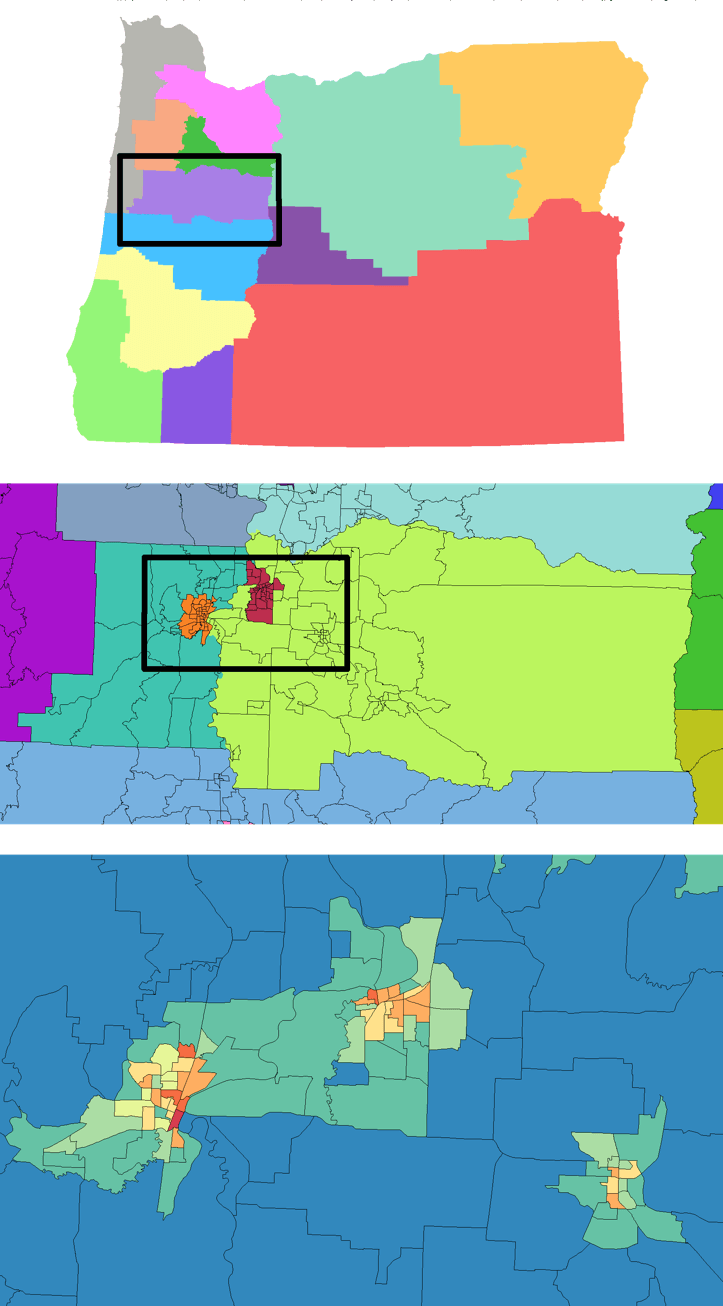
\includegraphics[scale=0.475]{aa/synthesis-geographies}
\caption{Synthesis geographies example}\label{fig:aa-synthesis-geographies}
\end{figure}

Each job in the PUMS file was also categorized based on these four categories; industries were coded by PECAS industry, occupations by both PECAS and CTTP codes, and a series of dummy variables indicated if a job was within one of the split industries, and if so, if it was one of the occupation groups considered to be a support function. (The definitions of support functions varied slightly by industry; the education occupation group is office support in most industries --- except in education industries, where it is the primary group of production workers.)

The employment by industry totals had a weight of 1; the other three target sets were proportions rather than absolute numbers of workers, so their targets were scaled appropriately. The weights developed were intended to emphasize matching the PECAS occupation groups ahead of the intensity groups or the CTPP groups. The relative weights were 2000, 500 and 250 respectively. 

The use of the industry split targets in the synthesizer means that industry management that occurs in office space was separated from line industry employment during the synthesis. Land use intensity (LUI) in any zone is calculated as a logged scale of combined population and employment per unit area. 
\begin{equation}\label{eq:6.41}
LUI_z = ln[(2.5*Employment_z  + Population_z)/Total Acres_z]
\end{equation}
\noindent This approach allows the share of management support workers to vary by industry-occupation combination and land use intensity. The assumed percent office support by industry and land use intensity used in the update are shown in Table \ref{tab:percent-office}. 

% Table 6-20 Assumed base year Percent Office Support by Industry and LU Intensity
\begin{table}
\centering
\caption{Assumed base year percent office support by industry and land use intensity}\label{tab:percent-office}
\begin{tabular}{lrrrrrrrr}
\hline
\multirow{2}{*}{Sector} & \multicolumn{8}{c}{Intensity range} \\
\cline{2-9}
& $<$-1 & -1 to 1 & 1 to 1.5 & 1.5 to 2 & 2 to 2.5 & 2.5 to 3.5 & 3.5 to 5 & $>$5 \\
\hline
Resources      & 10.0 & 59.2 & 68.5 & 74.7 & 79.6 & 83.5 & 87.0 &  90.0 \\
\gray Energy         & 25.0 & 25.3 & 27.2 & 31.9 & 40.5 & 54.0 & 73.6 & 100.0 \\
Construction   &  5.0 &  9.4 & 15.0 & 21.3 & 28.0 & 35.1 & 42.4 &  50.0 \\
\gray Manufacturing  &  5.0 & 10.6 & 19.7 & 31.0 & 43.8 & 58.1 & 73.5 &  90.0 \\
Wholesale      &  5.0 &  5.0 &  5.6 &  7.3 & 11.3 & 18.9 & 31.2 &  50.0 \\
\gray Retail         &  5.0 &  5.0 &  5.0 &  5.0 &  5.3 &  7.2 & 16.2 &  50.0 \\
Transportation & 10.0 & 12.9 & 19.5 & 28.9 & 40.9 & 55.2 & 71.6 &  90.0 \\
\gray Information    & 25.0 & 50.0 & 62.0 & 71.5 & 79.7 & 87.0 & 93.7 & 100.0 \\
Utilities      & 10.0 & 17.0 & 26.7 & 37.7 & 49.7 & 62.5 & 76.0 &  90.0 \\
\gray Education      &  5.0 &  6.0 &  8.9 & 13.6 & 20.1 & 28.3 & 38.3 &  50.0 \\
Government     & 25.0 & 25.3 & 27.2 & 32.0 & 40.7 & 54.2 & 73.7 & 100.0 \\
\hline
\end{tabular}
\end{table}

% Apparently A-F in this area, so need to reformat this to be in subsubsections

This production/support split could only be done for the zones in Oregon, as well as Clark County WA, where the zone system was fine enough to support this detailed level of land use intensity analysis. In the remainder of the halo, the zones are much larger --- frequently incorporating an entire urban area --- so that scale would distort the detailed land use intensity. A major city like Boise would have a downtown area with primarily office uses at high intensity, as well as large areas of moderate and lower intensity; because the entire city is one zone, it would be classified as having a moderate intensity, and the significant office workers downtown would be included in the region-wide total for moderate intensity zones, which would bias the office split in the more detailed areas. 

Instead, the halo areas (excluding Clark county WA, which has a finer zone system consistent with the Oregon zones) were assigned to a group with no control over the production/support split. However, because the zone system was relatively coarse, with a single zone for an urban area, all significant urban areas had an SOC occupation by Place (type c) target, that would control the employment by occupation for that individual zone. The cities where there was a SOC occupation by place target were Boise, Caldwell, Lewiston and Nampa, ID; and Kennewick, Longview, Pasco, Richland, Walla Walla and Yakima, WA.

\subsubsection{Agriculture and Forest (production and land)}
An inventory of forestry and agriculture land was available, and in initial runs of the employment synthesizer it was observed that many production (non-office) employees in Agriculture and Mining, Forestry and Logging were placed in several key urban zones where no such land was available. In order to solve the problem in the initial runs (employees located in several key urban zones where no such land was available), four constraints were added as targets in the employment synthesizer , based on zoning restrictions to help control the location of the agriculture and forest employment estimation:
\begin{itemize}
\item Constraint on the maximum number of land for all resource employees (agriculture and 
logging) in specific zones, calculated as follows:
\begin{equation}\label{eq:6.42}
Emp_{ag} * AcresPerEmp_{ag} + Emp_{for} * AcresPerEmp_{for} < \sum (AcresZoned in \textrm{rfor}, \textrm{rnatrs}, \textrm{xagfor})
\end{equation}
\item Constraint on the maximum number of land for agriculture only, as follows:
\begin{equation}\label{eq:6.43}
Emp_{ag} \cdot AcresPerEmp_{ag} < \sum (AcresZoned \in \textrm{rnatus}, \textrm{xagfor})
\end{equation}

\item Two additional constraints were used with the same purpose, but with less weight in the process, to reflect zones in which the condition was allowed to be less restrictive. This less restrictive weighting allowed the initial constraints to be overruled in selected low density regions outside of urban areas, often in the halo, which were found to be highly restrictive based strictly on the zoning coverage.
\end{itemize}

\subsubsection{Heavy and light industry employment}
Two constraints were added the employment synthesizer to control the total quantity and location of heavy industrial employment:  a list of zones where heavy industry was allowed and the total number of heavy industry employment. The list of alpha zones that allow heavy industry were obtained from the Oregon MPOs, as requested by ODOT in 2011. [58]  Only if the zone allowed heavy industry, were the following industries and occupations allowed in the allocation: 
\begin{itemize}
\item {Industries: ENGY\_elec\_hi, ENGY\_ngas\_hi, ENGY\_ptrl\_hi, MFG\_food\_hi, MFG\_htec\_hi, \\
MFG\_hvtw\_hi, MFG\_lvtw\_hi, MFG\_wdppr\_hi}
\item Occupations:  D1-Production Specialists, D2-MaintConstRepair Specialists, D3-ProtectTrans Specialists and D4-Blue Collar Unskilled
\end{itemize}

\subsubsection{Household Activity Targets}
Household counts by AA category (income and size, see Table \ref{tab:size-income} on page \pageref{tab:size-income}) by alpha zone were developed from US Census data. Household income and size data is available from US Census PUMS data for the years 2005 to 2009. PUMS data is available by PUMA which was tied to one or several beta zones. More complete data on household income and separately household size at the block group level from the the 2009 American Community Survey (ACS) 5-Year Estimates were used to develop marginals at the alpha-zone level. To develop detailed information at the alpha zone level, an iterative proportional fit method was used with the more detailed marginals and the PUMS multi-dimensional seed. 

\subsubsection{Import and Export Targets}

In a constrained AA run, imports and exports of commodities are constrained to flow through selected ``gateways.'' That is, the costs faced to import/export goods commodities reflects travel across the model network and assumed distances to various World Markets. As such, modelwide import and exports target quantities were identified for each World Market. Total modelwide imports and export to a particular market is provided by the NED module (in the base year consistent with 2009 IMPLAN data). Assumptions detailed below were used to develop the target market share of each commodity's imports and exports among these world markets. 

Information on the shares of imports/exports going to each World Market was identified from the FHWA Freight Analysis Framework (FAF3) dataset, with base year 2007. [51]  FAF is primarily based on the US commodity flow survey (CFS), Surface Transportation Board (STB) rail waybill data and US border crossing data, and provides freight flows in dollars and tons between 130 FAF zones across the U.S. Canada and Mexico, the remainder of the world is divided into six further world zones. In Oregon, there are two FAF zones, one for the 5-county Portland metropolitan area (Multnomah, Clackamas, Washington, Yamhill, and Columbia Counties) and another for the remainder of the state.FAF data distinguish seven different mode or mode combinations, and 43 SCTG commodities are specified. For international flows, the port of entry (i.e. the border crossing, marine port or air port) is provided as well. FAF2 was published in 2010 and has the base year 2007, with forecast years 2010 to 2040 in five-year increments. 

Shares of each commodity (in dollars) imported and exported to/from each World Market 6001 to 6005 were obtained from FAF3 flows of all modes (dropped ``pipeline'' and ``other and unknown''). Oregon's two FAF zones (``Portland Oregon'' and ``Oregon Remainder'') were treated as one zone for this analysis.

The Local World Market 6006 share was assumed based on expert judgment and 1997 and 2002 US Commodity flow average trip lengths by commodity. Those with large local (World Market 6006) market shares were typically low value-to-weight commodities with shorter average trip lengths. The resulting World Market shares by commodity are shown in Tables \ref{tab:assumed-imports} and \ref{tab:assumed-exports} and graphically in Figures \ref{fig:aa-world-imports} and \ref{fig:aa-world-exports}. As you can see, for many commodities, imports and/or exports are negligible.

%Table 6-21 Assumed Share of Imports from the World Markets
\begin{table}
\centering
\caption{Assumed share of imports from the world markets}\label{tab:assumed-imports}
\small
\begin{tabular}{clcccccc}
\hline
 & & \multicolumn{6}{c}{World market import share (rows sum to 100)} \\
\cline{3-8}
 & & N & NE & E & S & Port & Local \\
SCTG & Description & 6001 & 6002 & 6003 & 6004 & 6005 & 6006 \\
\hline
SCTG01 & Live animals and live fish & 91 & 0 & 3 & 2 & 0 & 5 \\
\gray SCTG02 & Cereal grains & 61 & 22 & 12 & 0 & 0 & 5 \\
SCTG03 & Other agricultural products & 28 & 3 & 23 & 33 & 8 & 5 \\
\gray SCTG04 & Animal feed and products, NEC & 40 & 3 & 40 & 11 & 1 & 5 \\
SCTG05 & Meat, fish, seafood and their preparations & 33 & 2 & 31 & 21 & 8 & 5 \\
\gray SCTG06 & Milled grain and bakery products & 37 & 4 & 32 & 22 & 0 & 5 \\
SCTG07 & Other prepared foodstuffs and fats and oils & 27 & 3 & 25 & 38 & 2 & 5 \\
\gray SCTG08 & Alcoholic beverages & 31 & 3 & 26 & 34 & 0 & 5 \\
SCTG09 & Tobacco products & \multicolumn{6}{c}{Combined with SCTG08} \\
\gray SCTG10 & Monumental or building stone & 33 & 9 & 0 & 23 & 0 & 35 \\
SCTG11 & Natural sands & 39 & 0 & 4 & 8 & 0 & 50 \\
\gray SCTG12 & Gravel and crushed stone & \multicolumn{6}{c}{Combined with SCTG11} \\
SCTG13 & Nonmetallic minerals, NEC & 18 & 1 & 29 & 26 & 5 & 20 \\
\gray SCTG14 & Metallic ores and concentrates & 4 & 0 & 58 & 0 & 4 & 35 \\
SCTG15 & Coal & 0 & 0 & 91 & 0 & 3 & 5 \\
\gray SCTG16 & Crude petroleum and bituminous oils & 0 & 0 & 0 & 0 & 0 & 0 \\
SCTG17 & Gasoline and aviation turbine fuel & 0 & 0 & 0 & 0 & 0 & 0 \\
\gray SCTG18 & Fuel oils & 0 & 0 & 0 & 0 & 0 & 0 \\
SCTG19 & Coal and petroleum products, NEC & 89 & 0 & 0 & 6 & 0 & 5 \\
\gray SCTG20 & Basic chemicals & 93 & 0 & 2 & 0 & 0 & 5 \\
SCTG21 & Pharmaceutical products & 89 & 0 & 5 & 0 & 0 & 5 \\
\gray SCTG22 & Fertilizers & 10 & 6 & 28 & 2 & 49 & 5 \\
SCTG23 & Chemical products and preparations, NEC & 5 & 1 & 82 & 1 & 5 & 5 \\
\gray SCTG24 & Plastics and rubber & 37 & 0 & 52 & 5 & 0 & 5 \\
SCTG25 & Logs and other wood in the rough & 70 & 0 & 21 & 2 & 2 & 5 \\
\gray SCTG26 & Wood products & 7 & 1 & 56 & 26 & 4 & 5 \\
SCTG27 & Pulp, newsprint, paper and paperboard & 14 & 2 & 53 & 23 & 4 & 5 \\
\gray SCTG28 & Paper or paperboard articles & 23 & 5 & 57 & 8 & 1 & 5 \\
SCTG29 & Printed products & 43 & 3 & 23 & 12 & 14 & 5 \\
\gray SCTG30 & Textiles, leather, articles of textiles or leather & 53 & 6 & 23 & 7 & 6 & 5 \\
SCTG31 & Nonmetallic mineral products & 47 & 3 & 21 & 23 & 1 & 5 \\
\gray SCTG32 & Base metal in various shapes & 16 & 3 & 53 & 21 & 2 & 5 \\
SCTG33 & Articles of base metal & 16 & 1 & 39 & 18 & 20 & 5 \\
\gray SCTG34 & Machinery & 31 & 1 & 23 & 32 & 8 & 5 \\
SCTG35 & Electronic, electrical, and office equipment & 21 & 2 & 35 & 33 & 5 & 5 \\
\gray SCTG36 & Motorized and other vehicles (including parts) & 19 & 4 & 42 & 18 & 11 & 5 \\
SCTG37 & Transportation equipment, NEC & 20 & 7 & 46 & 11 & 11 & 5 \\
\gray SCTG38 & Precision instruments and apparatus & 9 & 2 & 49 & 28 & 7 & 5 \\
SCTG39 & Furniture and fixtures, lighting, illuminated signs & 9 & 4 & 50 & 28 & 3 & 5 \\
\gray SCTG40 & Miscellaneous manufactured products & 5 & 0 & 72 & 5 & 13 & 5 \\
SCTG41 & Waste and scrap & 5 & 5 & 50 & 30 & 5 & 5 \\
\hline
\multicolumn{8}{l}{\footnotesize Note: Expert judgment used for local (6006) shares} \\
\end{tabular}
\end{table}

%Table 6-22 Assumed Share of Exports to the World Markets
\begin{table}
\centering
\caption{Assumed share of exports to the world markets}\label{tab:assumed-exports}
\small
\begin{tabular}{clcccccc}
\hline
          &             & \multicolumn{6}{c}{World market export share (rows sum to 100)} \\
\cline{3-8}
          &             & N    & NE   & E    & S    & Port & Local \\
Commodity & Description & 6001 & 6002 & 6003 & 6004 & 6005 & 6006  \\
\hline
SCTG01 & Live animals and live fish & 50 & 0 & 0 & 44 & 0 & 5 \\
\gray SCTG02 & Cereal grains & 42 & 0 & 0 & 0 & 52 & 5 \\
SCTG03 & Other agricultural products & 16 & 9 & 52 & 15 & 4 & 5 \\
\gray SCTG04 & Animal feed and products, NEC & 56 & 0 & 4 & 2 & 32 & 5 \\
SCTG05 & Meat, fish, seafood and their preparations & 63 & 1 & 11 & 18 & 3 & 5 \\
\gray SCTG06 & Milled grain and bakery products & 50 & 3 & 25 & 12 & 5 & 5 \\
SCTG07 & Other prepared foodstuffs and fats and oils & 23 & 3 & 48 & 20 & 1 & 5 \\
\gray SCTG08 & Alcoholic beverages & 46 & 2 & 26 & 21 & 0 & 5 \\
SCTG09 & Tobacco products & \multicolumn{6}{c}{Combined with SCTG08} \\
\gray SCTG10 & Monumental or building stone & 60 & 0 & 3 & 2 & 0 & 35 \\
SCTG11 & Natural sands & 36 & 0 & 12 & 2 & 0 & 50 \\
\gray SCTG12 & Gravel and crushed stone & \multicolumn{6}{c}{Combined with SCTG11} \\
SCTG13 & Nonmetallic minerals, NEC & 35 & 2 & 29 & 11 & 3 & 20 \\
\gray SCTG14 & Metallic ores and concentrates & 43 & 0 & 17 & 5 & 0 & 35 \\
SCTG15 & Coal & 2 & 0 & 47 & 0 & 46 & 5 \\
\gray SCTG16 & Crude petroleum and bituminous oils & 0 & 0 & 0 & 0 & 95 & 5 \\
SCTG17 & Gasoline and aviation turbine fuel & 92 & 0 & 3 & 0 & 0 & 5 \\
\gray SCTG18 & Fuel oils & 83 & 0 & 12 & 0 & 0 & 5 \\
SCTG19 & Coal and petroleum products, NEC & 85 & 1 & 6 & 2 & 1 & 5 \\
\gray SCTG20 & Basic chemicals & 23 & 1 & 37 & 18 & 16 & 5 \\
SCTG21 & Pharmaceutical products & 7 & 10 & 64 & 12 & 2 & 5 \\
\gray SCTG22 & Fertilizers & 30 & 1 & 36 & 13 & 15 & 5 \\
SCTG23 & Chemical products and preparations, NEC & 16 & 1 & 64 & 11 & 4 & 5 \\
\gray SCTG24 & Plastics and rubber & 33 & 4 & 29 & 25 & 4 & 5 \\
SCTG25 & Logs and other wood in the rough & 10 & 0 & 36 & 10 & 39 & 5 \\
\gray SCTG26 & Wood products & 16 & 5 & 42 & 31 & 1 & 5 \\
SCTG27 & Pulp, newsprint, paper and paperboard & 16 & 3 & 22 & 48 & 6 & 5 \\
\gray SCTG28 & Paper or paperboard articles & 32 & 3 & 6 & 53 & 1 & 5 \\
SCTG29 & Printed products & 26 & 2 & 45 & 21 & 1 & 5 \\
\gray SCTG30 & Textiles, leather, articles of textiles or leather & 54 & 4 & 23 & 13 & 1 & 5 \\
SCTG31 & Nonmetallic mineral products & 39 & 10 & 29 & 16 & 0 & 5 \\
\gray SCTG32 & Base metal in various shapes & 48 & 3 & 20 & 22 & 2 & 5 \\
SCTG33 & Articles of base metal & 30 & 3 & 44 & 17 & 1 & 5 \\
\gray SCTG34 & Machinery & 27 & 4 & 42 & 17 & 4 & 5 \\
SCTG35 & Electronic, electrical, and office equipment & 10 & 3 & 47 & 31 & 3 & 5 \\
\gray SCTG36 & Motorized and other vehicles (including parts) & 40 & 4 & 26 & 21 & 4 & 5 \\
SCTG37 & Transportation equipment, NEC & 69 & 0 & 17 & 2 & 7 & 5 \\
\gray SCTG38 & Precision instruments and apparatus & 4 & 1 & 46 & 39 & 4 & 5 \\
SCTG39 & Furniture and fixtures, lighting, illuminated signs & 29 & 9 & 32 & 24 & 1 & 5 \\
\gray SCTG40 & Miscellaneous manufactured products & 24 & 4 & 48 & 18 & 1 & 5 \\
SCTG41 & Waste and scrap & 8 & 0 & 2 & 3 & 36 & 50 \\
\hline
\multicolumn{8}{l}{\footnotesize Note: Expert judgment used for local (6006) shares} \\
\end{tabular}
\end{table}

\begin{figure}   % Formerly Figures 6.7 and 6.8
\centering
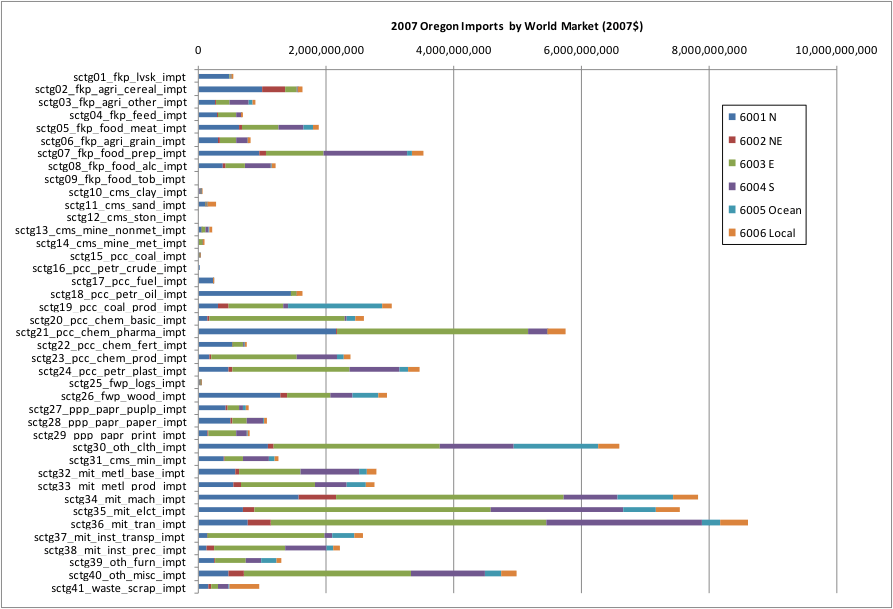
\includegraphics[width=6.0in]{aa/world-imports}
\caption{Assumed world market imports market share}\label{fig:aa-world-imports}
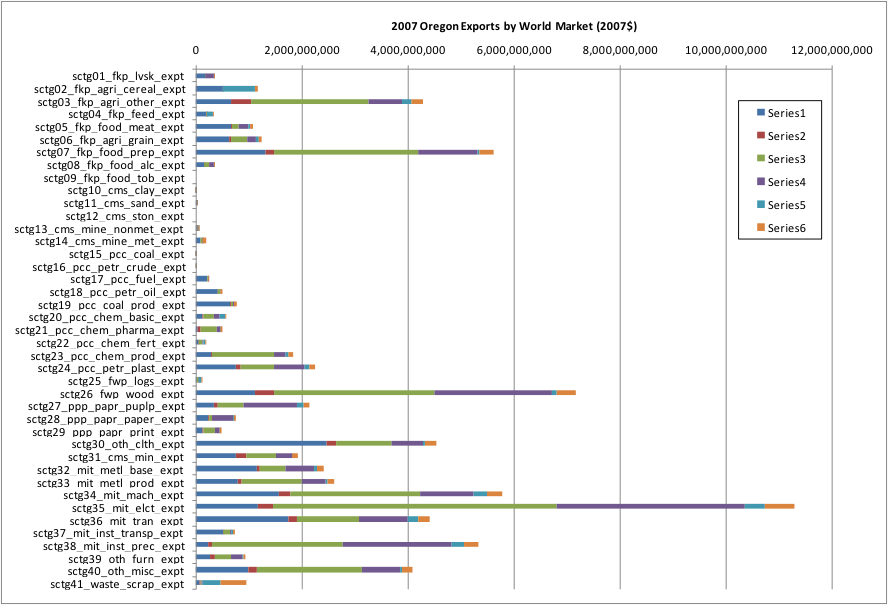
\includegraphics[width=6.0in]{aa/world-exports}
\caption{Assumed world market exports market share}\label{fig:aa-world-exports}
\end{figure}
 
\subsection{Trip Length Targets}\label{sec:aa-trip-length-targets}
Observed trip length distances were collected to compare with AA commodity flow outputs. An automated trip length calibration routine uses targets in the file histogramsI.csv and outputs comparable distributions in histograms.csv, and resulting updates to dispersion parameters in CommoditiesI.csv.

\subsubsection{Commodity Trip Distances}
For freight, the FAF data provides 2007 average distances by SCTG commodity, as shown in Figure \ref{fig:aa-faf-distances}. This includes only trips within Oregon by value for all modes (dropped ``Pipeline'' and ``Other unknown'' modes). FAF3 has two Oregon zones, with intrazonal distances assumed to be 25 miles for ``Portland Oregon'' FAF zone and 215 miles for ``Oregon Remainder'' FAF zone (based on average of non-Portland OD pairs mileage table [50]) and 153.72 miles between them. Because of this coarse geography and the fact that FAF, based on the US CFS, primarily addresses long-distance travel and average distances vary significantly between years, the data are not ideal. It is most important to calibrate the trips internal to the model area, excluding imports and exports. 

\begin{figure}    % Formerly Figure 6.9
\centering
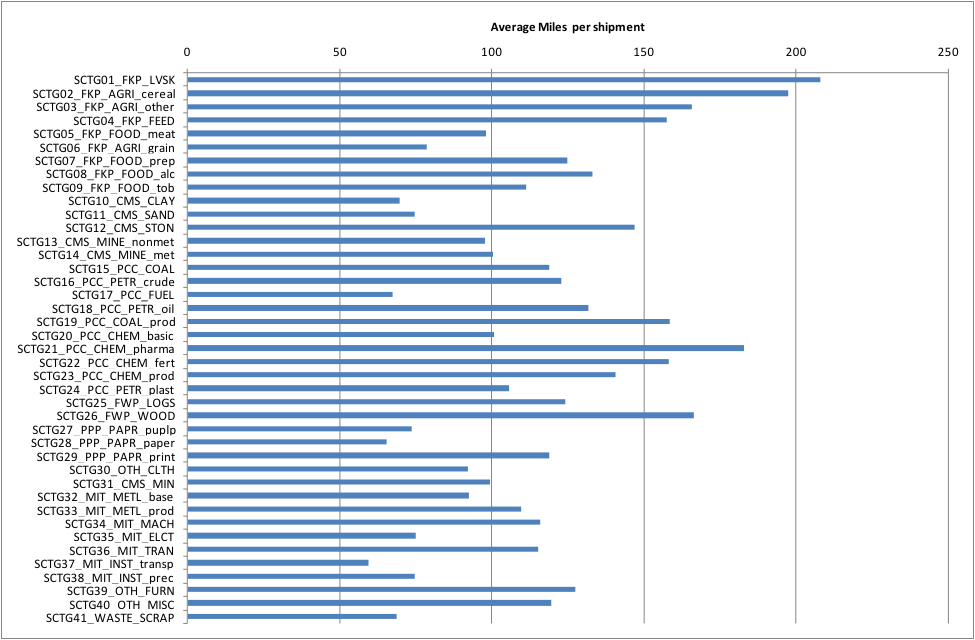
\includegraphics[width=6.0in]{aa/faf-distances}
\caption{FHWA FAF3 average commodity trip distance in Oregon}
\label{fig:aa-faf-distances}
\end{figure}

\subsubsection{Person Trip distance distribution}
The combined 1994 and 1996 Oregon Travel Behavior Surveys collected household activity data from the four Oregon MPO areas (Metro, M-WVCOG, LCOG and RVCOG) and eight additional rural Oregon counties (Clatsop, Coos, Deschutes, Josephine, Klamath, Lincoln, Malheur and Umatilla) as shown in Figure \ref{fig:aa-obts-map}. Eighty percent of the sampled trips were by auto. 

\begin{figure}[!t]    % Formerly Figure 6.10
\centering
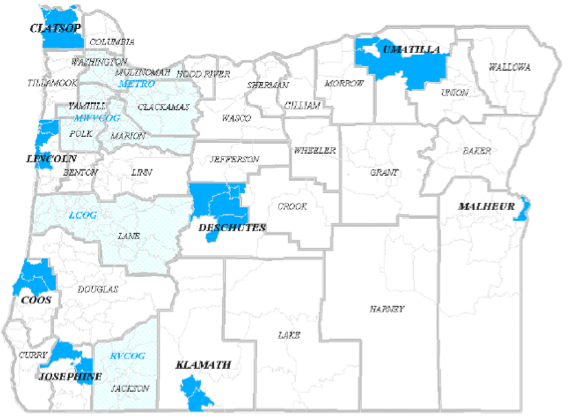
\includegraphics[width=4.0in]{aa/otbs-map}
\caption{Map of Oregon Travel Behavior Survey surveyed areas}
\label{fig:aa-obts-map}
\end{figure}

These observed trip lengths will be used to assess AA person flow outputs. Survey data on the first link of each trip tours is broken out by purpose with work trips further delineated by occupation. These will be compared to work commute and personal services trip distances, output from the AA module. Services are broken into personal and business categories, based on their primary activity, as shown in Table \ref{tab:activity-industry} (page \pageref{tab:activity-industry}). The personal distance distributions are shown in Figure \ref{fig:aa-personal-distance}. The figure indicates that most Oregon person tips are less than five miles. Work trips are the shortest in length. Portland has less of the shortest work trips (less than 2.5 miles). This concurs with a separate source, Portland DOT fact sheet that reports an average (home-based) work trip of 6.6 mile in Portland.

\begin{figure}    % Formerly Figure 6.61
\centering
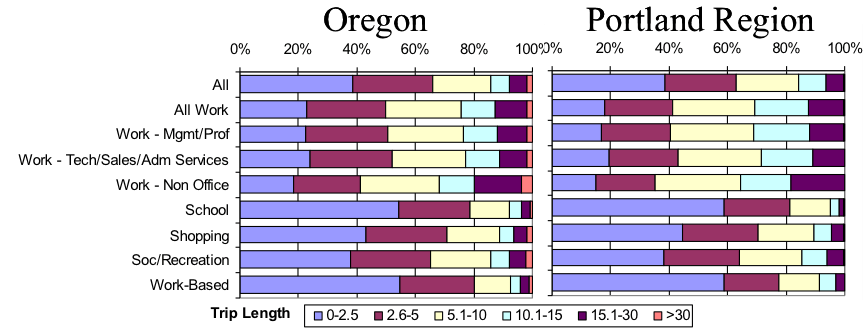
\includegraphics[width=6.0in]{aa/personal-distance}
\caption{Map of Oregon Travel Behavior Survey surveyed areas}
\label{fig:aa-personal-distance}
\end{figure}

Average business-related service trip lengths will be generated by combining the 1994/1996 Oregon household survey data with Ohio Business Establishment survey data. Business-related service trips were isolated from the Oregon data by industry and will be checked against Ohio data. 

\subsection{Floorspace Price Targets} 
Floorspace prices by building type provide general targets to assess residential and commercial floorspace prices inAA outputs by beta zone. The 2000 census provided data on residential space, while commercial rents were obtained from a sample of observed sales.  

\subsubsection{Residential Floorspace Price Targets}
2000 Census data were used to estimate residential floorspace rents. The estimates included two sets of values; a zone-specific base rent, and a set of local effect factors that adjust this base rent to reflect the local influences that act at a geographic level smaller than the zone system. The latter is useful in a land use micro-simulation model, such as the PECAS Space Development (SD) module. By separating the two elements, a more unbiased estimate can be obtained for the zonal rent, used as the AA target. 

A full discussion of the theory and mathematics behind this estimation is discussed in [53]. In general, a synthetic population of housing units was created for the entire model region. It was derived through a simulated annealing process using 2000 Census SF3 (Summary file 3) data at a block group level, which served as marginals, matched with 2000 PUMS (5 percent) disaggregate data. American Community Survey data was used to convert Census number of rooms to building sqft. A gross rent for the entire block group (SF3) was used to scale the PUMS-based rents. 

The second step isolated three local rent effects: the distance to major roads, the distance to water, and the local density. These were all calculated by census block. The first two assumed a 10 mile buffer analyses, while the density measure was defined as the number of housing units within 0.25 miles of the block. Each block was assumed to have a constant density of housing units, and the portion of each block within the buffer was used to determine this value. 

An ordinary least squares procedure with a linear model was used to estimate the local effects shown in Table \ref{tab:res-rent-regression}. The constant or base price in each zone is show graphically in Figure \ref{fig:aa-base-rents}.

\begin{figure}[!t]
\centering
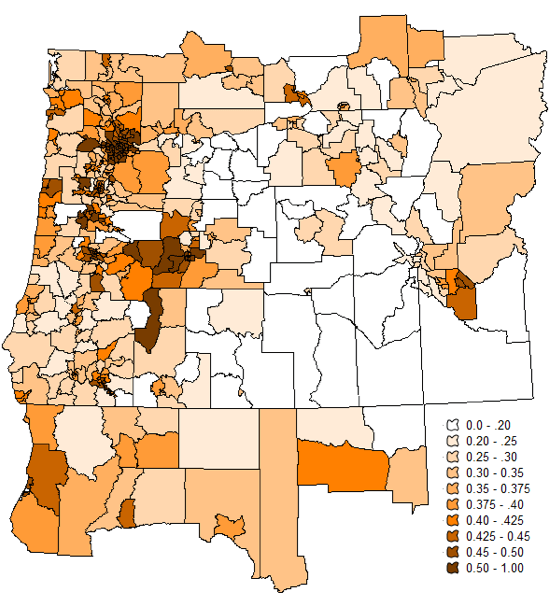
\includegraphics[scale=0.6]{aa/figure6-7alt}   % figure number mis-numbered in original text
\caption{Base rent (\$/sqft) for modeled area}\label{fig:aa-base-rents}
\end{figure}

\begin{table}
\centering
\caption{Residential rent regression}\label{tab:res-rent-regression}
\begin{tabular}{lrr}
\hline
Regression & Coefficient & Intercept \\
\hline
MH & 1.103516503 & 960996.2 \\
\gray RRMH & 0.327002266 & 1797385 \\
SFD & 1.341969751 & -1245254 \\
\gray RRSFD & 0.574700142 & 150677.6 \\
\hline
\end{tabular}
\end{table}

The higher values for mobile home and multifamily can be attributed to the larger size per unit for these dwelling types. The constant for age is negative reflecting the expected reduction of value of buildings with age. The constant for density is positive, which may reflect multiple trends. In a large city, accessibility can be thought of as the distance to the downtown, shopping centers and services. However, in smaller towns, accessibility is as much the distance to Main Street and to other towns and cities.Water has a larger parameter than proximity to major road in these estimations. All rents are in the same money units used by the census, dollars per month, calculated on a per square foot basis.

The base prices by zone are consistent with expectations; the rural areas of eastern Oregon and the halo have the lowest rent values, and the major urban areas have the highest, and especially the south-western suburbs. The high base rents for the rural areas to the west of Bend are unexpected. The two highest rent zones in the area also have a very low number of observations, which is likely playing a role in these values. A revisiting of the rent prices in these areas by a more manual intervention may be necessary.

When used as targets for AA calibration, the base price for each beta zone was modified by the average value of each local variable (density, distance to water, distance to road, from the 2000 Census) using the rent modified coefficients of Table \ref{tab:res-rent-regression}. This modified base price was extended to the various floorspace types based on regressions of 1998-PI floorspace target data relative to the average price for that type. The regression results are given in Table \ref{tab:resulting-rent-parameters}, and the resulting parameters applied to the modified base for each type is given in Table \ref{tab:residential-modifiers}, with average rents by region shown in Figure \ref{fig:average-res-rents}. For comparison with AA outputs (ExchangeResultsI.csv ``price''), the prices are in units of amortized annual prices (\$/sqft) in 2009 dollars.

\begin{table}
\centering
\caption{Resulting residential rent parameters applied to modified base rent}
\label{tab:resulting-rent-parameters}
\begin{tabular}{lrr}
\hline
Combined & Coefficient $\times$ base (\$M) & +Intercept \\
\hline
RES-AT & 0.902685344 & 0 \\
\gray RES-MF & 1.325467507 & 0 \\
RES-MH & 1.205775939 & 960996.2 \\
\gray RES-RRMH & 0.357304547 & 1797385 \\
RES-SFD & 1.341969751 & -1245254 \\
\gray RES-RRSFD & 0.574700142 & 150677.6 \\
\hline
\end{tabular}
\end{table}

\begin{figure}
\centering
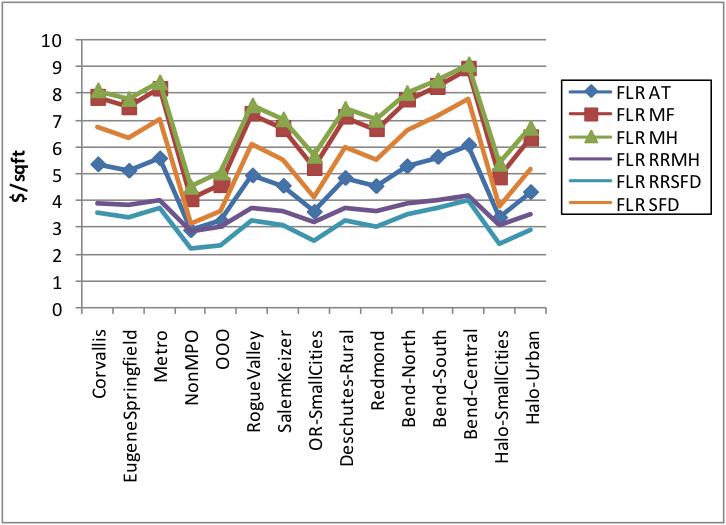
\includegraphics[scale=0.45]{aa/figure6-8alt}   % Mis-numbered in original document
\caption{Average residential rents (\$/sqft) by region}\label{fig:average-res-rents}
\end{figure}

\begin{sidewaystable}    % Table 6-23 Residential Rent Modifier Parameters
\centering
\caption{Residential rent modifier parameters}\label{tab:residential-modifiers}
\begin{tabular}{llcccc}
\hline
 & & & Estimated & T-ratio for & Corresponding \\
Parameter & Form & RefDValue & value for $a_g$ & estimated $a_g$ value & value for $\omega_g$ \\
\hline
Attached single family dummy & Constant & n/a & -0.0973 & 8.50 & 0.907 \\
\gray Multifamily dummy & Constant & n/a & 0.3255 & 54.53 & 1.384 \\
Mobile home dummy & Constant & n/a & 0.0927 & 8.67 & 1.097 \\
\gray Density & Reversed Power & 1 & 0.000103 & 10.47 & -0.000103 \\
Distance to water (feet) & Shifted exponential & 2640 & 0.0395 & 5.10 & 0.0395 \\
\gray Distance to road (feet) & Shifted exponential & 2640 & 0.0872 & 5.47 & 0.0872 \\
\hline
\end{tabular}
\end{sidewaystable}

\subsubsection{Commercial Floorspace Price Targets}
Observed non-residential prices were collected for key locations within the study area to compare with AA commodity price outputs. Floorspace prices were obtained from Real Estate Market reports for key urban areas (Bend-Deschutes [54], Portland [55], Salem-Keizer, Eugene-Springfield, Rogue Valley, Corvallis) and selected rural areas (Oregon Small Cities) within Oregon. Urban areas within the halo adopted average of Salem, Eugene, Rogue Valley and Corvallis. Non MPO in Oregon or the halo assumed 90 percent of the prices of the Oregon Small Cities data. All data was collected for the years 2009-2011 and converted to 2009 dollars.

Selected rent data, typically from the web for one or a couple areas within each region (Deschutes-Bend)was downloaded and processed. A linear regression was then performed for each of the basic space types for which data was available: office, retail, warehouse and industrial. In Deschutes County (Bend) ``warehouse'' floorspace prices were not available, so the same Office-Whse-Ind price relationship found in non-Metro MPOs was assumed. In Portland, Retail was not available, so 110 percent of the average Salem, Eugene, Rogue Valley, Corvallis Retail rates were assumed.

The variation in the observed basic type prices across the regions is shown in Figure \ref{fig:aa-basic-floorspace-prices}. These regional prices were then disaggregated to zones. In the Portland area, all zones had observed prices for the basic types which were used directly. In some cases, a few holes were filled by adopting prices from adjacent areas. In other areas, the relationship of prices across zones within the regions from 1998 PI-based floorspace price targets were used to arrive at average zone prices. To do so, average 1998 prices for all types in each MPO was generated. Then the ratio of the zonal target price to the average price in this 1998 data was calculated. This 1998 price ratio was applied as a scalar to the observed 2009 average MPO prices to arrive at zone-specific prices. 

\begin{figure}    % Formerly Figure 6.14
\centering
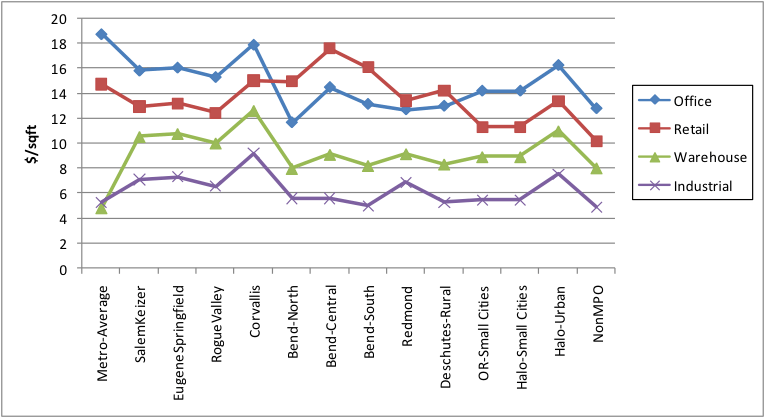
\includegraphics[width=6.0in]{aa/basic-floorspace-prices}
\caption{Basic floorspace prices by region}
\label{fig:aa-basic-floorspace-prices}
\end{figure}

Once these basic floorspace types were covered, they were extended to cover the other AA nonresidential space types. Accommodations, Government Support, K12, Hospital, and Institutional adopted ``Office'' prices. Heavy and Light industry both adopted ``Industrial'' prices. Agriculture and Logging lands assumed \$15,000 per acre. The same 1998-zonal pattern scaling noted above was also used on these non-basic floorspace types, which was often not the same pattern as the basic type (e.g., office and accommodation price scalars might differ). No zone's price was allowed to drop below a minimum price set at 50 percent of the $ExpectedPrice$ defined in AA input file CommoditiesI.csv. Figure \ref{fig:aa-retail-floorspace-prices} shows the average floorspace price for all types across the regions.

\begin{figure}    % Formerly Figure 6.15
\centering
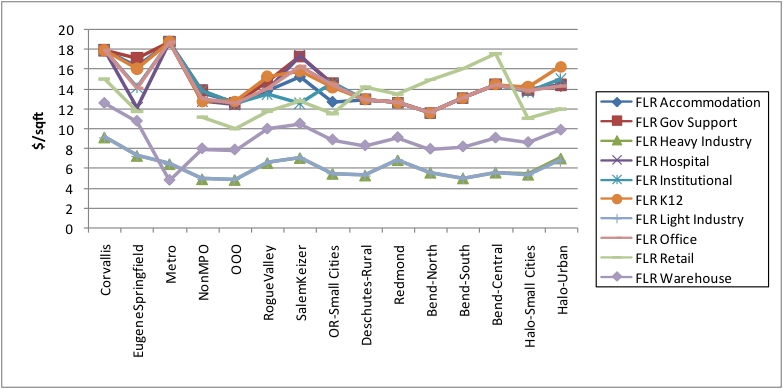
\includegraphics[width=6.0in]{aa/retail-floorspace-prices}
\caption{Retail and industry floorspace prices}
\label{fig:aa-retail-floorspace-prices}
\end{figure}

For comparison with AA outputs (ExchangeResultsI.csv ``price''), the prices are in units of amortized annual prices (\$/sqft) in 2009 dollars. 

\subsection{Commodity and Labor Flow Targets}

\subsubsection{Commodity Flow Targets}
The FHWA Freight Analysis Framework (FAF3)provides 2007 data on the flow (in dollars) of commodity movements in, out, and within the state (see \S\ref{sec:aa-trip-length-targets} for data description used in commodity trip distances). This target data, summarized in Table \ref{tab:aa-faf3-flows}, can be compared to AA flow matrices for each commodity (selling\_SCTG*.zmx). Note that these data are independent of the IMPLAN data used in NED that is used to define the overall quantity of flow in NED and AA. As such, it might be more useful to compare relative values only.

%Table 6-26 2007 FAF3 Flows, in, out, within Oregon (2007$)
\begin{table}
\centering
\caption{FAF3 flows in, out, and within Oregon, in 2007 dollars}
\label{tab:aa-faf3-flows}
\small
\begin{tabular}{lrrrr}
\hline
Commodity & OR imports & OR exports & Within OR & \% local \\
\hline
SCTG01\_FKP\_LVSK & 513,050,125 & 339,096,909 & 779,891,461 & 48 \\
\gray SCTG02\_FKP\_AGRI\_cereal & 1,545,018,337 & 1,111,557,953 & 1,488,285,000 & 36 \\
SCTG03\_FKP\_AGRI\_other & 845,320,641 & 4,065,851,489 & 2,911,841,018 & 37 \\
\gray SCTG04\_FKP\_FEED & 664,711,113 & 326,681,597 & 503,585,800 & 34 \\
SCTG05\_FKP\_FOOD\_meat & 1,788,122,165 & 1,022,702,207 & 1,181,970,878 & 30 \\
\gray SCTG06\_FKP\_AGRI\_grain & 769,284,881 & 1,188,071,419 & 1,020,120,942 & 34 \\
SCTG07\_FKP\_FOOD\_prep & 3,350,738,063 & 5,343,447,509 & 3,082,694,560 & 26 \\
\gray SCTG08\_FKP\_FOOD\_alc & 726,571,165 & 286,444,705 & 1,447,450,506 & 59 \\
SCTG09\_FKP\_FOOD\_tob & 412,899,085 & 48,404,201 & 379,892,196 & 45 \\
\gray SCTG10\_CMS\_CLAY & 37,812,001 & 4,620,401 & 350,062,484 & 89 \\
SCTG11\_CMS\_SAND & 59,452,701 & 1,843,201 & 109,890,700 & 64 \\
\gray SCTG12\_CMS\_STON & 74,850,001 & 16,003,401 & 415,626,908 & 82 \\
SCTG13\_CMS\_MINE\_nonmet & 167,393,601 & 47,053,001 & 90,622,700 & 30 \\
\gray SCTG14\_CMS\_MINE\_met & 58,180,301 & 132,194,389 & 2,076,300 & 1 \\
SCTG15\_PCC\_COAL & 13,515,601 & 983,501 & 427,400 & 3 \\
\gray SCTG16\_PCC\_PETR\_crude & 3,001 & 1,219,101 & 38,400 & 3 \\
SCTG17\_PCC\_FUEL & 226,259,305 & 226,376,893 & 4,383,043,934 & 91 \\
\gray SCTG18\_PCC\_PETR\_oil & 1,539,768,017 & 472,512,945 & 2,224,503,352 & 53 \\
SCTG19\_PCC\_COAL\_prod & 2,871,767,635 & 729,500,901 & 1,316,688,412 & 27 \\
\gray SCTG20\_PCC\_CHEM\_basic & 2,458,215,841 & 551,407,317 & 324,965,204 & 10 \\
SCTG21\_PCC\_CHEM\_pharma & 5,466,607,993 & 472,270,065 & 1,875,274,588 & 24 \\
\gray SCTG22\_PCC\_CHEM\_fert & 720,969,461 & 177,694,701 & 308,502,492 & 26 \\
SCTG23\_PCC\_CHEM\_prod & 2,267,072,461 & 1,753,345,167 & 1,108,440,494 & 22 \\
\gray SCTG24\_PCC\_PETR\_plast & 3,286,987,819 & 2,143,697,529 & 1,453,720,704 & 21 \\
SCTG25\_FWP\_LOGS & 36,885,701 & 100,623,601 & 31,785,300 & 19 \\
\gray SCTG26\_FWP\_WOOD & 2,808,749,743 & 6,817,147,673 & 4,381,969,470 & 31 \\
SCTG27\_PPP\_PAPR\_puplp & 737,031,217 & 2,037,525,443 & 533,900,984 & 16 \\
\gray SCTG28\_PPP\_PAPR\_paper & 1,017,084,169 & 715,366,965 & 1,420,600,320 & 45 \\
SCTG29\_PPP\_PAPR\_print & 761,453,121 & 456,695,801 & 1,059,349,408 & 47 \\
\gray SCTG30\_OTH\_CLTH & 6,261,516,743 & 4,320,955,781 & 2,416,852,162 & 19 \\
SCTG31\_CMS\_MIN & 1,190,854,565 & 1,824,193,491 & 3,267,382,790 & 52 \\
\gray SCTG32\_MIT\_METL\_base & 2,641,014,089 & 2,287,099,785 & 1,937,415,332 & 28 \\
SCTG33\_MIT\_METL\_prod & 2,624,619,071 & 2,487,989,665 & 3,014,642,272 & 37 \\
\gray SCTG34\_MIT\_MACH & 7,437,560,381 & 5,501,173,891 & 10,637,128,772 & 45 \\
SCTG35\_MIT\_ELCT & 7,163,601,851 & 10,729,985,303 & 5,043,549,094 & 22 \\
\gray SCTG36\_MIT\_TRAN & 8,184,706,297 & 4,192,043,773 & 3,915,328,320 & 24 \\
SCTG37\_MIT\_INST\_transp & 2,441,527,765 & 710,298,437 & 208,094,604 & 6 \\
\gray SCTG38\_MIT\_INST\_prec & 2,107,658,451 & 5,065,495,549 & 445,596,792 & 6 \\
SCTG39\_OTH\_FURN & 1,225,939,257 & 895,793,341 & 791,336,400 & 27 \\
\gray SCTG40\_OTH\_MISC & 4,738,775,085 & 3,890,551,997 & 1,854,959,488 & 18 \\
SCTG41\_WASTE\_SCRAP & 477,999,877 & 475,325,865 & 1,385,731,402 & 59 \\
\gray SCTG43 Mixed miscellaneous$^a$ & 4,500,276,391 & 6,907,573,625 & 9,058,693,880 & 44 \\
\hline
Total & 86,221,825,088 & 79,878,820,488 & 78,163,933,223 & 32 \\
\hline
\multicolumn{5}{l}{\footnotesize a. Included in FAF3 data, but not used by AA.}
\end{tabular}
\end{table}


\subsubsection{Labor Flows Targets}
Labor flow targets from 2000 US Census PUMS data, in units of wages by occupation between PUMA (home-to-place of work) were process as a target for AA labor flows. PUMS data was chosen over county-level US Census CTPP data since CTPP is classified by wages per household not occupation used in AA. This target can be compare to SWIM2 AA output flow matrices (\$labor\_occupations\$.zmx), collapsing beta zones to match PUMAs and occupations, and adjusting for 2009 dollars. Further discussion of this PUMS dataset can be found in \S\ref{sec:aa-zonal-activity-targets} with the employment by industry, including Figure \ref{fig:aa-synthesis-geographies} showing maps of PUMA boundaries within the study area.

In the PUMS data, place of residence is ``Puma'' and place of work is ``POWPuma''. Blank POWPumas were dropped, indicating that the person is Civilian employed with a job but not at work, currently unemployed, or not in labor force. In aggregating wage data, it was weighted by the number of employed persons. 

\section{Initial Calibration}\label{sec:aa-initial-calibration}
A formal four tier calibration strategy was employed to assess the fit of the AA module in the second stage (S2) of the calibration process, with additional informal checks by ODOT. The set of calibration procedures that was used is described below, along with further improvements that could be made to the calibration.
\begin{enumerate}
\item Convergence and Zonal Activity Totals
\begin{enumerate}
\item Zonal constants were fine-tuned to match zonal activity targets (household counts and worker activity dollars).
\item Modelwide imports and exports were calibrated and constants in the world market adjusted to match these targets.
\item AA was assembled and run to convergence. After the results of this run were reviewed, the activity dispersion parameters (in ActivitiesI.csv) were updated. The industry parameters were borrowed from Baltimore, where they had been calibrated to elasticity on space use.  The household parameters were borrowed from California, where they were based on combinations of nesting rules and elasticity tests. Labor occupation choice was investigated further to determine whether there was appropriate spatial labor specialization around job locations, using Census PUMA level targets for occupations. The model was rerun to convergence constrained to zonal activity totals. The prices were high for some non-residential space types, a problem that was revisited in floorspace price calibration.
\end{enumerate}
\item Trip lengths were checked against previous 1998 targets for services and labor, and updated FAF3 goods trip length targets. A semi-automated routine was developed to perform the calibration, and the AA input files were updated. Modifications that had been previously made to the transport coefficients to match trip length targets were revisited, to understand overall flow length distributions and their economic implications. The census question details regarding trips to work were investigated; very long distances between home and workplace are unlikely to be reported in Census, which focuses on the usual journey to work.  Further investigation could occur using other labor market surveys. At this stage the labor flow distances in PECAS seem appropriate but are somewhat longer than observed average trip lengths, and it is suggested that this be addressed further in the transportation models so that trip-to-work distributions can be shorter than labor-flow distributions.
\item Prices: reasonable values for floorspace and labor prices:
\begin{enumerate}
\item Technology option cluster weights were calibrated so that household chose their technology cluster points in the correct amounts (use of dwelling type, dwelling size, make of labor occupations) and so that industries chose the correct amount of space overall (use of labor and floorspace).
\item Floorspace inventory were adjusted so the resulting model reproduced floorspace price targets, while maintaining the correct amount of activity within the zone (zonal activity constants calibration). An automated script was used to adjust the initial synthesized floorspace quantities by Alpha Zone. This script automates the process of finding a best match to both inventory and price data while retaining the zonal activity of Step 1. This calibration script was was instrumental in discovering a mismatch between housing data and census population data. The resulting model's match to rent targets and total inventory targets was mapped and plotted and discussed by the team, and the matches were deemed appropriate.  Vacancy rates may also be reviewed in full model calibration.
\end{enumerate}
\item Technology option choice dispersion parameters were adjusted for households based on occupation choice targets. In general, they were not changed much from their previous values from December of 2012.
\item Commodity flows
\begin{enumerate}
\item Labor flows can be checked against POWPUMA-PUMA flow targets by occupation.
\item Goods commodity flows into/out of/through the state can be compared against FAF3 targets in total and/or by aggregated commodities where possible.
\end{enumerate}
\item Check household trends over time by comparing SPG household size (SynPopP.csv + SynPopH.csv) trends over time, to Portland Metro forecast/other sources.
\end{enumerate}

The calibration targets used to assess the model fit during calibration were previously listed in Table \ref{tab:aa-calibration-targets}. The following AA Validations of special interest to ODOT. The first two are part of the calibration noted above, while the last one can be included if ODOT leads the comparison effort:
\begin{itemize}
\item High Prices of selected space types (Office, Warehouse, Light Industry, Retail, Grade School, Government Support) are current PI-ALD issue in SWIM2. Some spaces will likely not be market sensitive and/or limited quantities result in counterintuitive prices (schools, government, hospitals), but prices for common space types should not be unreasonably high. (See AA calibration step 5)
\item Long Distance Commuting is important for GHG reduction strategies. Not a focus in prior PI calibration (when comparing CTPP county-county labor flows, $R^2$ was high since matched larger short commutes, but did not match well against smaller long distance flows and HH survey not capture either). New OHAS survey data that includes long commutes will help, possibly Census OnTheMap data as well. (See AA calibration step 3). AA does not represent commuting distance, only a financial relationship between an employer and an employee. PT uses the financial relationship to forecast commuting trips. Properly accounting for long distance commute trips may require an adjustment of PT which is beyond the scope of the current project.  
\item Matching HHSize changes: PI/AA is calibrated to households, not population, so household size trends are not controlled. In Oct 2010 model runs, SWIM2 predicted reasonable HH forecasts compared to Portland Metro model runs, but overall population was larger due to SWIM2 forecast of larger HH sizes (consistent with Census trends for increased workers per HH). SWIM2 also predicted Eastern Oregon average household size would grow over time, while the rest of Oregon shrunk.  Additionally, a ``stepped'' growth in household size changes was observed (might be due to recent ALD changes). ODOT is encouraged to update these comparisons with the updated SWIM2 spatial models during calibration, where issues can be discussed appropriate action can be taken, if required.
\end{itemize}

Calibration Step 3 is discussed in more detail below:

\subsubsection{Iterative floorspace calibration}

The use of synthesized floorspace inventory directly proved to be excessively large (high vacancy rates) and resulted in homogenous prices across all zones. As a result, an involved process is used to iteratively trim the floorspace quantities while constraining the process to meet the following targets:
\begin{itemize}
\item Modelwide vacancy rates by floorspace type from 2000 Census (residential) and mid-1990s real estate sales reports (nonresidential).
\item Modelwide activity use of each residential floorspace type from 2000 Census PUMS(sqft/HH).
\item Alpha zone-level floorspace prices by floorspace type (\$/building sqft) from mid-1990s real estate sales reports (selected urban areas) and early 1990s Tax Assessor Data used in SWIM1 model development (outside urban areas, converted from \$/land sqft).
\end{itemize}

The process involves iteratively running the AA module as follows. The resulting floorspace more accurately represented both floorspace price variations and vacancy rates: 
\begin{itemize}
\item Reduce floorspace inventory to match target modelwide vacancy rates by floorspace type (alpha zone).
\item Iteratively calibrate AA modelwide activity use of floorspace type (offset parameters) while constraining to alpha zone activity targets. To save runtime, this was first done at a county zone level and then the county offsets were transferred to the more disaggregate beta zone level for fine tuning.
\item As needed, adjust the floorspace inventory to match target modelwide floorspace price targets. This tended to reduced price outliers caused by the above steps, but worked against reducing vacancy rates.
\item Repeat additional adjustments to floorspace inventory to match target modelwide vacancy rates (and to a lesser extent zonal floorspace prices), as needed, repeating this multi-step process until vacancy rates were within the target range and prices were reasonable.
\end{itemize}

This process was applied to all nonresidential floorspace types and single-family (SFD) residential floorspace type. Residential calibration was complicated by the fact that all household types are allowed to use multiple floorspace types. However since residential space in the model is dominated by SFD type, the above adjustments were made to SFD only. The inventory of other residential floorspace types was derived from the resulting SFD space based on 2000 Census mix of dwelling units in each alpha zone.

\section{Further Calibration}
Additional rounds of calibration were performed after data discrepancies were found and corrected. First, after initial calibration revealed a mismatch between housing data and population data in Clark County, Washington, the following calibration steps were performed on the corrected model:
\begin{enumerate}
\item Household cluster weights were calibrated so that household activities were allocated to clusters in the correct proportions. This was done using an autonomous script that iteratively ran AA and adjusted the weights to bring the proportions closer to the targets. After calibration, all cluster amounts matched their targets.
\item Floorspace inventory was adjusted to better match the observed space prices without deviating too much from the existing floorspace quantities from previous calibration. This was achieved by assigning each quantity and price target a ``tolerance'' indicating how far the calibration script would allow the modeled value to deviate from the target. Since large interactions occurred between cluster weight calibration (step 1) and floorspace calibration, these two processes were run alternately until they both converged, as described below. For some space types (e.g. office, retail), only small adjustments were needed. For other types, where prices started far from the targets, larger adjustments were needed; for example, heavy industry space was decreased by half in some zones to control inflated prices in the model. In all space types, the overall fit to the targets improved.
\item Trip lengths for goods, which had deviated from their targets during other calibration steps, were re-calibrated against the FAF3 goods trip length targets. An autonomous script ran AA repeatedly, increasing the location choice dispersion parameter for each commodity to decrease the average trip length and vice versa. Labor and service trip lengths were not included in this step because dispersion parameter adjustments alone could not match the targets.
\end{enumerate}

The second round of recalibration was done after correcting errors in the household counts. Only floor space calibration was performed at this stage, using the same price targets as before. The space targets were adjusted to remove small out-of-place floorspace amounts (such as rural residential space in urban areas) and to better fit the distribution of observed activities. 

\subsubsection{Alternating cluster weight and floorspace calibration}
An automated script was developed to repeatedly run the cluster weight and floorspace calibration processes in an alternating fashion. The initial runs used relaxed convergence criteria so that they took less time, while later runs restored more demanding convergence criteria to ensure an accurate calibration.

This alternation was done because the cluster weights were calibrated assuming the original floorspace quantities. Changing the floorspace amounts affected the supply of residential floorspace, which altered the proportions assigned to each cluster. The effect on cluster distribution was so dramatic that AA would sometimes not converge at all. After alternating the two calibration routines, all household cluster amounts matched their targets, and the overall fit to floorspace quantity and price targets was improved.

\section{S3 Parameters}
When the full SWIM2 model is undergoing calibration, the following parameters may be adjusted to improve AA and overall model performance:
\begin{itemize}
\item Inertia parameters for activity location by activity type $\alpha_{inertia}$ and $InertiaConsta$.
\item Floorspace import function parameters (for calculating floorspace import functions based on floorspace inventory).
\item Multipliers for the influence of specific commodity buying and selling utility values on production location utility ($\phi$b,c,a and $\phi$s,c,a).
\item Affect of production utility and consumption utility on location utility ($\alpha_{prod,a}$ and 
$\alpha_{cons,a}$).
\item Utility of non-modeled production and non-modeled consumption ($U_{nmc}$ and $U_{nmp}$).
\item Utility function dispersion parameter for allocation of by-product substitutes and input substitutes made and used by each activity ($\lambda_{m,a}$ and $\lambda_{u,a}$).
\end{itemize}

\chapter{Person Travel (PT) Module}\label{sec:pt-module-chapter}
The Person Transport (PT) module generates travel for all households resident in Oregon and the halo region. Work trips are based on labor flows from the AA module and influenced by travel times, distances and costs by all modes of transport from VISUM, and intermediate accessibilities calculated by PT. PT consists of two jointly run sub-components: Short Distance Transport (SDT) which predicts all regular work commutes regardless of length and non-commute travel patterns less than or equal to 50 miles in length; and Long Distance Transport (LDT) which predicts non-commute travel patterns greater than 50 miles. PT returns a list of short and long-distance trips with attributes including origin and destination alpha zone, start time, duration and mode. PT also provides zone-to-zone O-D matrices for person auto and (inter- and intra-city) transit trips by time period and short distance tour mode choice and destination choice logsums by household category.

\section{Theoretical Basis}
For inspiration in designing the PT SDT module for modeling the sequence and timing of activities, we looked to tour-based micro-simulation model development work completed in Portland, Oregon \citep{cambridge99}; San Francisco, California \citep{jonnalagadda02}; the Ohio Statewide Model \citep{parsons10}; the Mid-Ohio Regional Planning Commission (MORPC) model \citep{vovsha04}, and work then under development in Sacramento \citep{bowman05}. The Portland, San Francisco, and Sacramento model systems are based on the day-pattern modeling approach developed by \cite{bowman95}. The model imposes a hierarchical system of activity typology, with work and school tours at the top of the typology, followed by shop, social/recreational and other activities.

The day-pattern model consists of a large multinomial logit model (114 alternatives total) that predicts the primary activity type (as defined by the hierarchical structure) and its nominal location (at-home versus out-of-home), the number of intermediate stops on the primary tour and the number and purpose of ``secondary'' tours. These secondary tours were further defined (i.e., number of stops on secondary tours and number of secondary tours if 2+ tours) by Monte Carlo sampling according to observed distributions. In the San Francisco and Portland models time periods are discretely defined (five total) and determined by another series of logit models. Tour mode and ``primary'' destination are determined simultaneously and intermediate stop locations are determined using the additional or ``out-of-direction'' distance, that the intermediate stop incurs between the tour origin (home or work) and primary destination. 

The PT module in the second-generation Oregon StateWide Integrated Model (SWIM2) departs from previous work in Portland, San Francisco, and Sacramento in primarily three significant ways:
\begin{enumerate}
\item The day-pattern model uses observed patterns as alternatives in a multinomial logit framework. The model parameters interact with the characteristics of the person/household and the characteristics of the pattern to determine the utility for each observed pattern. The model is segmented by person type, which achieves the two-fold goal of reducing the number of alternatives for each sub-model and eliminates irrelevant choices given a person's work and student status. 
\item The trip mode choice occurs at two stages within the Oregon StateWide Integrated Model system. At the first stage, trips are allocated to drive-alone, shared-ride 2, shared-ride 3+, walk, bike, transit walk or transit drive mode. Another layer of trip mode choice occurs on-the-fly within path-building for transit trips; a transit trip can either walk all the way or use some combination of transit modes. Trip mode choice is restricted by the primary mode of the tour and is probabilistic according to the characteristics of the person choosing the mode, the level of service characteristics of the modes allowed for the tour mode and the characteristics of the tour and day-pattern.
\item Time in SWIM2 was originally treated as a logit time-of-day choice model. Developments in the MORPC tour-based models and the Sacramento model design blend hazard-based duration models within a logit framework, offering the best of both worlds; a model that can be sensitive to level-of-service matrices within specific time periods, while offering a fairly detailed representation of time. In operation, the hazard duration model had limitations and was replaced with a discrete choice framework.\footnote{SDT initially used hazard-based duration models treating time as a continuous variable, providing opportunities to overcome differences in peak period definitions for different urban areas throughout Oregon and allowed for long distance travel to occur throughout multiple time periods in the day. However, the models do not provide for a convenient way to represent congestion effects on schedule and their use in Oregon uncovered limitations due to the assumption of parametric baseline hazards, which led to their replacement with a discrete choice model framework.} The Oregon models operate at a one-hour time resolution level.
\end{enumerate}

A long-distance transport model (PT LDT) was developed, based on Ohio Statewide Model (OSMP) framework and the Ohio long distance travel survey. LDT leverages the tour-based methods of the SDT model with some simplifying assumptions. In the long-distance models, all tours are assumed to start at home and in cases where multiple stops are chained together, the farthest stop is considered the primary destination and all intermediate stops are ignored. For example, if a business tour is actually anchored at work, the model treats the home location as the tour origin. This convention was adopted partly due to data limitations. The Ohio long-distance survey only collected travel over 50 miles. Thus, short trips such as travel between home and work were not included in the survey and would have to be synthesized without a gain in overall model value, particularly since distance from home to work is typically short relative to the length of the trip. Additionally, the location of intermediate stops were not specifically gathered as part of the survey effort, thought it is likely that many additional stops are incidental stops for gas or food at highway exits and have little effect on mode choice or route choice. The case of additional substantive stops, such as combining a trip to visit relatives with a vacation to a second city is a consideration for future improvements. The model chooses which component of the full trip will occur on the actual simulation day.

Enhancements to the Oregon PT model design have come from common software code used in both Oregon and Ohio statewide models. Ohio enhancements now employed in Oregon include the Long Distance Transport (LDT) module and specifically within SDT include the logit time-of-day choice model (which replaces the initially-estimated hazard-based activity duration model), additional market segmentation and some generalization of the pattern choice model. These enhancements ensure a consistent representation of travel in Oregon while providing the opportunity for efficiencies in model calibration and application.

\section{Quantity Definitions and Categories}
The PT SDT module operates strictly at the alpha zone level, while the PT LDT module operates at the alpha zone level internally, while external destinations are assigned to one of the 12 external station zones at the edge of the model area (zones 5000-5012), shown previously in Table \ref{tab:external-stations} and Figure \ref{fig:swim2-external-stations} (page \pageref{fig:swim2-external-stations}). SDT does not assign any trips to the external stations.

PT SDT uses categories shown in Tables \ref{tab:sdt-tour-def} through \ref{tab:sdt-person-types}, as well as the occupation fields in Table \ref{tab:service-categories} (page \pageref{tab:service-categories}) to define activities, modes, workers, households and persons. PT LDT uses the categories shown in Table \ref{tab:ldt-trip-purposes}. The seven person trip activity definitions used in the SDT travel patterns of the day pattern and tour time-of-day models are shown in Table \ref{tab:sdt-tour-def}. Additionally, these codes (minus home) serve as the primary destination or trip purpose, used in the PT tour primary destination choice model. The PT tour and trip mode choice model assumes the mode options shown in Tables \ref{tab:sdt-tour-modes} and \ref{tab:sdt-trip-modes}, respectively. The various combinations of modes that can make up a trip are summarized in Table \ref{tab:sdt-allowable-modes}. The PT workplace location choice model uses the occupations, previously defined in Table \ref{tab:service-categories} and the market segments of Table \ref{tab:sdt-market-segments}. The PT tour mode choice also uses the market segments listed in Table \ref{tab:sdt-market-segments}. The PT day pattern model uses the SDT person types of Table \ref{tab:sdt-person-types}.

\begin{table}  % 7-1
\centering
\caption{PT SDT activity/tour primary destination definitions}\label{tab:sdt-tour-def}
\begin{tabular}{cl}
\hline
Code & Description \\
\hline
H & Home \\
\gray W & Work (including second job), without a work-based subtour \\
B & Work (including second job), with a work-based subtour \\
\gray C & School \\
S & Shop \\
\gray R & Social/recreation \\
O & Other (including pickup or drop-off activity) \\
\hline
\end{tabular}
\end{table}

\begin{table}  % 7-2
\centering
\caption{PT SDT tour mode categories}\label{tab:sdt-tour-modes}
\begin{tabular}{c L{4.9in}}
\hline
Tour mode & Description \\
\hline
Auto Driver & Any trip on tour is auto driver, no trips are school bus \\
\gray Auto Passenger & All trips on tour are passenger or non-motorized (including school bus for school tours) \\
Passenger-Transit & Any trip outbound is auto passenger and any trip inbound is walk transit \\
\gray Transit-Passenger & Any trip outbound is walk transit and any trip inbound is auto passenger \\
Walk & Only walk trips on tour \\
\gray Bike & Bike trips on tour, no motorized trips \\
Walk Access Transit & Walk transit trip on tour, no drive transit trips on tour. Includes tours with passenger and transit on same half tour \\
\gray Drive Access Transit & Any trip on tour is drive transit \\
\hline
\end{tabular}
\end{table}

\begin{table}  % 7-3
\centering
\caption{PT SDT trip mode categories}\label{tab:sdt-trip-modes}
\begin{tabular}{lccll}
\hline
Trip code & SDT & LDT & Trip mode & Definition \\
\hline
DA & X & X & Drive-Alone & Single-occupant auto \\
\gray SR2 & X & X & Shared-Ride 2 & 2 person occupant auto \\
SR3P & X & X & Shared-Ride 3+ & 3+ person occupant auto \\
\gray WALK (1) & X & & Walk & Walk \\
BIKE (1) & X & & Bicycle & Bicycle \\
\gray TRANSIT\_WALK & & X & Walk-Transit & Walk-Access Transit \\
TRANSIT\_DRIVE & & X & Drive-Transit & Auto-Access Transit \\
\gray SCHOOL\_BUS (1) & X &  & School bus & School bus (not assigned to the network) \\
AIR & & X & Drive-Air & Drive-access air travel within the model area \\
\gray HSR\_DRIVE & & X & Walk-HSR & Drive-access intercity rail \\
HSR\_WALK & & X & Drive-HSR & Walk-access intercity rail \\
\hline 
\multicolumn{5}{l}{(1) School Bus and non-motorized modes (walk and bicycle) are not assigned to the network} \\
\end{tabular}
\end{table}

\begin{table}  % 7-4
\centering
\caption{PT SDT Allowable Trip Modes Within Tour Mode}\label{tab:sdt-allowable-modes}
\begin{tabular}{l C{0.5in} C{0.63in} C{0.63in} C{0.5in} C{0.5in} C{0.63in} C{0.5in}}
\hline
\multirow{2}{*}{Tour mode} & \multicolumn{7}{c}{Trip Modes} \\
\cline{2-8}
& Drive-alone & Shared Ride 2 & Shared Ride 3+ & Walk & Bike & Walk-transit & Drive-transit \\
\hline
Auto driver & X & X & X \\
\gray Auto passenger & & X & X & X & & & \\
Walk & & & & X \\
\gray Bicycle & & & & X & & & \\
Walk-transit & & & & X & & X \\
\gray Transit-passenger & & X (return only) & X (return only) & X & & X (outbound only) & \\
Passenger-transit & & X (outbound only) & X (outbound only) & X & & X (return only) \\
\gray Drive-transit & & & & X & & X & X \\
\hline
\end{tabular}
\end{table}

\begin{table} % 7-5
\centering
\caption{PT SDT market segments (in current 2000 dollars)}\label{tab:sdt-market-segments}
\begin{tabular}{cl}
\hline
Code & Market Segment \\
\hline
0 & HHincome $<$\$30,000, autos $=$ 0 \\
\gray 1 & HHincome $<$\$30,000, autos $<$ HHWorkers \\
2 & HHincome $<$\$30,000, autos $\ge$ HHWorkers \\
\gray 3 & \$30,000 $\le$ HHincome $<$\$60,000, autos $=$ 0 \\
4 & \$30,000 $\le$ HHincome $<$\$60,000, autos $<$ HHWorkers \\
\gray 5 & \$30,000 $\le$ HHincome $<$\$60,000, autos $\ge$ HHWorkers \\
6 & HHincome $\ge$\$60,000, autos $=$ 0 \\
\gray 7 & HHincome $\ge$\$60,000, autos $<$ HHWorkers \\
8 & HHincome $\ge$\$60,000, autos $\ge$ HHWorkers \\
\hline
\end{tabular}
\end{table}

\begin{table}  % 7-6
\centering
\caption{SDT person types}\label{tab:sdt-person-types}
\begin{tabular}{cll}
\hline
Code & Person type & Definition \\
\hline
0 & Pre-school & All persons less than 6 years old \\
\gray 1 & Grade/High School & All persons older than 5 and younger than 18 \\
2 & Worker & All students older than 17 and not students \\
\gray 3 & College student & All persons older than 17 \\
4 & Non-worker & All persons older than 17 and not students nor workers \\
\hline
\end{tabular}
\end{table}

It is useful to define several terms as they are used in PT such as day pattern, tour, intermediate stop and primary destination and tour mode. The activity day pattern consists of a sequence of characters (referred to as a ``word'') that fully describes a person's activities during the forecast day. The number of tours, their sequence, their purpose and the number, type and sequence of stops on each tour can be determined from the word pattern.

Each character in the pattern represents an activity at a nominal location, implying that a trip is required for every activity with the exception of the first at-home activity of the day. The activity pattern consists of tours, which are sequences of activities that start and end at home. For example, the activity pattern word ``howhrh'' consists of two tours for the following sequence of activities:
\begin{itemize}
\item Tour 1: Home $\rightarrow$ other $\rightarrow$ work $\rightarrow$ home
\item Tour 2: Home $\rightarrow$ recreate $\rightarrow$ home
\end{itemize} 

\noindent Note that intermediate at-home activities serve as breakpoints between tours and that multiple at-home activities are modeled as a single activity.

A sequence of activities that starts and ends at work is known as a work subtour or work-based tour. In the pattern model these subtours are identified with a ``b'' and are fully contained within a home-based tour. For example, the activity pattern ``hbhoh'' consists of the following tours and activities:
\begin{itemize}
\item Tour 1: Home $\rightarrow$ Work-based $\rightarrow$ Home
\item Tour 2: Work $\rightarrow$ Other-Work
\item Tour 3: Home $\rightarrow$ Other $\rightarrow$ Home
\end{itemize}

Each tour contains a primary destination, which was selected from among all tour destinations according to the following hierarchical structure and which defines the purpose of the tour:
\begin{itemize}
\item Work
\item School
\item Shop
\item Social/Recreational
\item Other
\end{itemize}

For students, the highest priority activity is School, followed by Work. When a tour includes multiple high priority activities of the same type, the one with the longest duration was chosen as the primary activity. Therefore, the purpose of a stop cannot be of higher priority than the tour primary destination.

Each tour is allowed to include at most one intermediate stop between home and the primary tour activity (the outbound leg) and at most one intermediate stop between this activity and home (the inbound leg).In order to reduce VMT loss when estimating and calibrating the models, the tour retains from the survey data the intermediate stop requiring the largest distance deviation between home and the primary destination. Stops are allowed to choose destinations further away from home than the primary destination, but like primary destinations they are restricted to be within 50 miles of home.

The tour mode is the mode used to reach the primary destination and is chosen before the location of the intermediate stops is known.The mode(s) for trips within a person's tour can be different from the tour mode, but they are consistent with it. For example, if the tour mode is passenger, none of the trip modes can be drive alone.

\begin{table}  % 7-7
\centering
\caption{LDT trip purposes and patterns}\label{tab:ldt-trip-purposes}
\begin{tabular}{lll}
\hline 
Category & Label & Description \\
\hline
Trip purpose & Household & Travel in which entire household participates \\
& Work-Related & Individual business travel \\
& Other & Individual travel for non-work purposes \\
\hline
Trip pattern & Complete Tour & Entire tour is complete on simulation day \\
& Begin Tour & Tour departs on the simulation day \\
& End Tour & Tour returns on the simulation day \\
& Away & Person is out-of-town on the simulation day \\
& No Tour & Travel occurs on a different day \\
\hline
\end{tabular}
\end{table}

It should be noted that PT was originally developed in Oregon, then applied in Ohio where it was further enhanced, and then reinstated back to Oregon to achieve the advancements in the Ohio version. As such, SWIM2 is estimated primarily with Ohio long distance and short distance travel survey data, supplemented with Oregon household survey data (see \S\ref{sec:pt-s1-s2}). Additionally unlike the rest of SWIM2, Ohio uses 2000 dollars and cents monetary units. As such, the 1990 dollars of all SWIM2 inputs are translated to 2000 units for use in PT and then translated again, if needed to produce SWIM2 outputs in 2009 dollars in order to remain consistent with the rest of the model. 

\section{Component Models}
An overview of the PT SDT and LDT models is provided in Figure \ref{fig:ptmodel}. Both operate in a micro-simulation framework, and rely on the attributes of the synthetic population (from SPG) and travel skims (from VISUM). The SDT model also uses work flows (in 2009 dollars) from the AA module. 

% Figure 7.1 Person Transport Model Flow Diagram
\begin{figure}[!b]
\centering
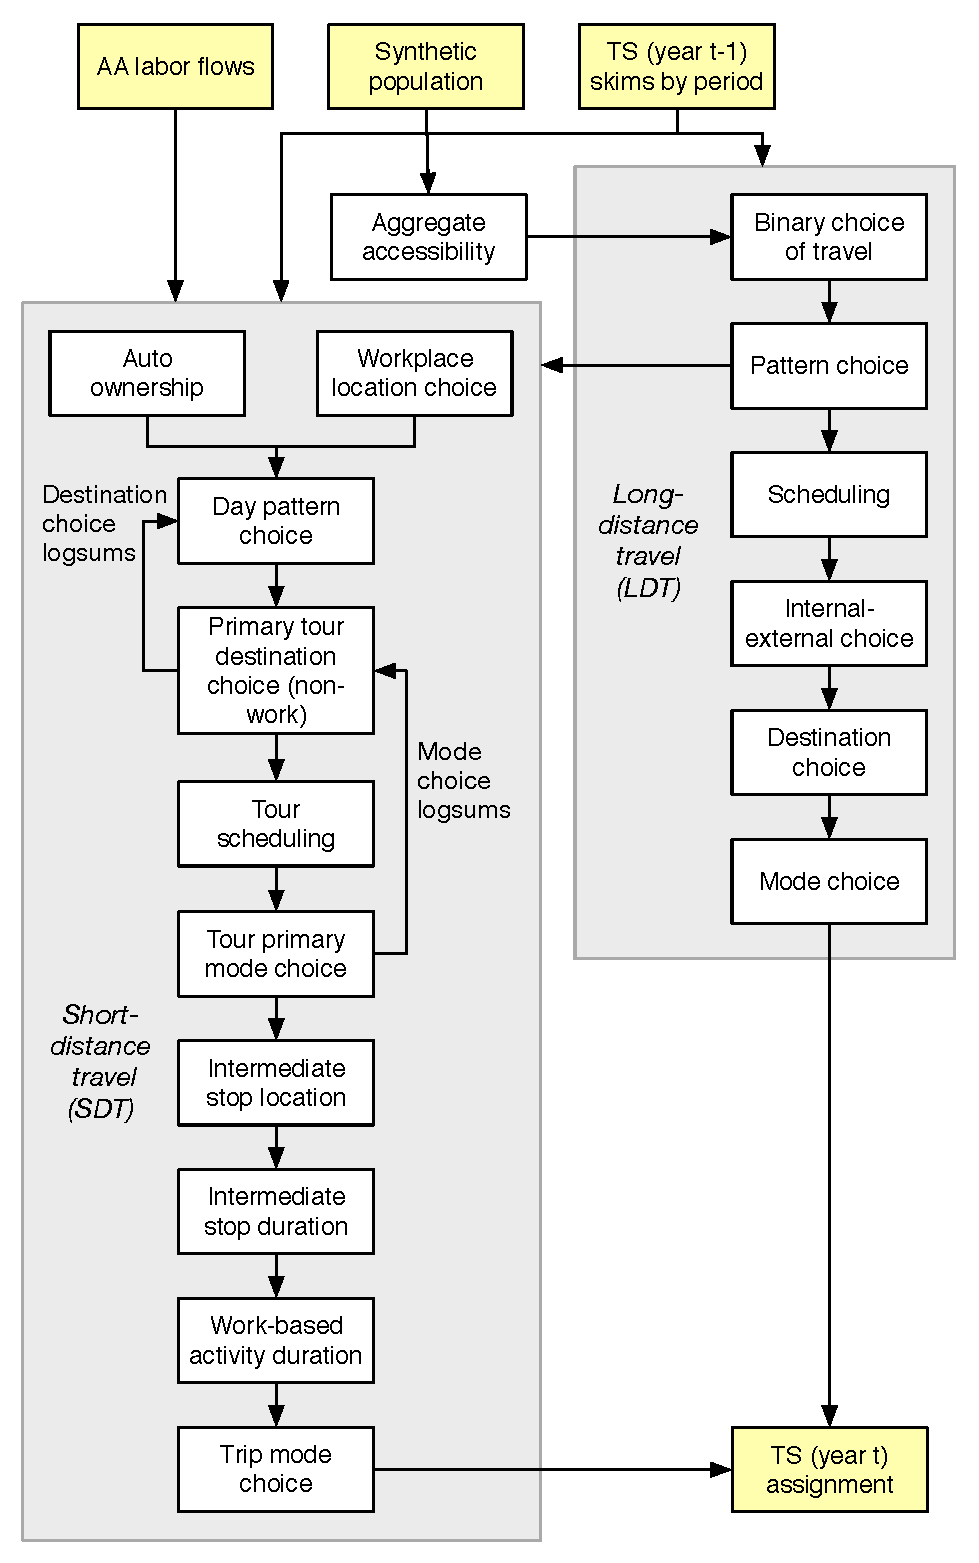
\includegraphics[scale=0.65]{pt/ptmodel}
\caption{Person transport (PT) model flow diagram}\label{fig:ptmodel}
\end{figure}

The SDT model generates mode choice and destination choice logsums as a measure of accessibility for use by the LDT model (and AA module). This allows for a lower probability of long-distance travel if the short-distance destinations are more attractive. In turn, the LDT choice of whether or not to engage in long-distance travel is fed back to the SDT models. Persons who are traveling out-of-town are assumed to not engage in short-distance travel (LDT only) while the remainder are assumed to travel typical short-distance travel patterns (SDT only). 

Short-distance and commute travel (SDT) consist of a series of (mostly) discrete choice models, which represent the trip-making decision as a sequential process, in the following order:  auto ownership, work place location, activity day pattern, primary non-work activity location, work-based activity location, tour schedule, tour mode, intermediate stop location, intermediate stop duration, work-based activity duration and trip mode. 

The behavior of long-distance travel (LDT) is modeled in six steps. First, each eligible traveler is given the choice of whether or not to engage in long-distance travel during a two-week period. For those who travel during the two-week period, the pattern model predicts the type of travel that occurs on the actual simulation day. Third, the tours are scheduled to a time-of-day. Next, each tour is evaluated to determine whether the destination will be internal or external to the model area boundary. Finally, a specific destination and then a mode are chosen.

The resulting trips from both models are assigned together in VISUM to the same networks, although intra-city transit networks are used for SDT trips and inter-city transit networks for LDT trips. PT SDT also outputs prior period mode choice and destination choice logsums based on the prior period's travel costs (skims, 3 year lag) for use in the current year by the PT and the AA module. PT also produces current year synthetic population attributes regarding auto ownership and work alpha zone. 

These PT SDT and LDT components are detailed in the remainder of this section.

\subsection{SDT Aggregate Accessibilities}\label{sec:sdt-aggregate-accessibilities}
Initial aggregate accessibilities are calculated and used by both SDT and LDT components. Tour mode choice logsums and tour destination choice logsums are used as measures of travel accessibility by the LDT and the SDT components of the PT module as well as the AA module. The destination choice logsum represents the overall ability of travelers to access any destination. The logsums are important to PT LDT because they allow the models to capture the effect that people who have access to many destinations within a short distance are less likely to need to make long distance trips. Within SDT, these accessibilities influence the day pattern model, the auto ownership model, the tour destination choice model and the tour scheduling model. They are referred to as aggregate accessibilities because they are a function of the origin and destination zone attributes only. The logsums are calculated in the same fashion as the utilities for the SDT tour mode choice and destination choice model, but excluding all terms that are person-related. The mode choice logsums are however segmented by household market.\footnote{Refer to Sections \ref{sec:sdt-primary-tour-destination} and \ref{sec:sdt-tour-mode-choice} for a detailed description of the PT SDT tour mode choice and destination choice models.}

\subsection{LDT binary choice of travel}
Urban modelers often complain that travel is difficult to predict because it planned on a time scale longer than one day. This is especially true of long-distance travel. To capture this longer-term planning, long-distance tours in LDT are generated over a two-week period, rather than over a single day. The binary choice of travel model, predicts the probability of engaging in each type of long-distance travel during a two-week period. Note that the binary choice of travel model predicts the presence of travel for each purpose (Table \ref{idunno}) during the time window, not the quantity. The presence could be part of a tour (i.e., departing during the travel window and returning at a later date), it could be a complete tour or it could be multiple tours. Also, an individual can have travel for multiple purposes occur during the two-week window. Given the presence of travel, the LDT tour pattern model will determine what actually happens on the model day. The variables in the linear utility for the binary choice of travel for each purpose include the following:
\begin{itemize}
\item Household attributes (workers, autos, household size, household income, presence of students, single family home)
\item Person attributes (worker occupation, student, sex, age)
\item Accessibility (SDT destination logsums)
\item Constant
\end{itemize}

\subsection{SDT auto ownership model}\label{sec:sdt-auto-ownership}
The PT SDT tour mode choice model requires the number of autos owned by each household. Since the SPG module does not output (not controlled for) auto ownership information in the synthetic population (from SPG2), the PT SDT auto ownership model predicts the total number of vehicles owned by each household. It is a discrete choice multinomial logit model applied to each resident household in the synthetic population. The resulting auto count is output with the household ID for future analysis in addition to other SPG-produced synthetic population attributes. 

In the auto ownership model the household is assigned ownership of zero (base), one, two, or two or more autos. A logit model is used to assign probabilities to the alternative categories for the Monte Carlo process to use in setting this attribute for an individual household. The utility function includes the following variables:
\begin{itemize}
\item Household attributes of composition and wealth (household size, number of employed persons, household income)
\item Accessibility from the home location to the rest of the model area
\item Aggregate destination choice logsum (see Section \ref{sec:sdt-aggregate-accessibilities})
\end{itemize}

The destination choice logsum is calculated as follows, where $p$ denotes an origin zone and $q$ a destination zone:
\begin{equation}\label{eq:7.1}
DCLogsum_p = \sum exp \left[ \alpha \times Dist_{pq} + \beta \times Time_{pq} + log(Emp_q) \right]
\end{equation}
where:
\begin{align*}
DCLogsum_p &= \text{destination choice logsum for home zone $p$ to all destination zones} \\
Dist_{pq} &= \text{distance from zone $p$ to zone $q$} \\
Time_{pq} &= \text{peak period travel time from zone $p$ to zone $q$} \\
Emp_q &= \text{total employment in destination zone $q$} \\
\alpha, \beta &= \text{parameters to be estimated}
\end{align*}

\noindent PT outputs the resulting auto ownership assignment (number of autos) in the household data file, which contains one record per household, as in the synthetic population. 

\subsection{SDT workplace location choice model}\label{sec:sdt-workplace-location-choice}
This model assigns a workplace location for every worker, by sampling from the labor flow probability matrices developed by the AA module. If a work tour is generated for the worker, the work alpha zone chosen through this method will become the primary destination of the work tour and serve as the anchor location for any work-based tours. The workplace location model is applied to each employed person in the synthetic population.

The workplace location (alpha zone) choice for each worker is based on the following factors:
\begin{itemize}
\item Labor dollar flows by occupation between beta zones
\item Quantity of labor produced and consumed in each alpha zone
\item Mode choice logsums, as a measure of travel cost, between alpha zones
\end{itemize}

\noindent The model applies a matrix expansion process to convert labor dollar flows by occupation between beta zones to flows between alpha zones. The formula for this conversion is as follows:
\begin{equation}
F_{a_m} = F_{\beta_{ij}} \times {{QL_m} \over {\sum_{m \in M(i)} QL_m}} \times {QL_n \over {\sum_{n \in N(j)} QL_n}} \times {{exp(\lambda LS_{mn})} \over {\sum_{m \in M(i)} \sum_{n \in N(j)}exp({\lambda LS_{mn}})}}
\end{equation}
where:
\begin{align*}
m &= \text{origin zones in the alpha zone system} \\
n &= \text{destination zones in the alpha zone system} \\
i &= \text{origin zones in the beta zone system} \\
j &= \text{destination zones in the beta zone system} \\
M(i) &= \text{set of all alpha zones contained within a specific beta zone $i$} \\
N(j) &= \text{set of all alpha zones contained within a specific beta zone $j$} \\
F_{mn} &= \text{labor flow from alpha zone $m$ to alpha zone $n$} \\ 
F_{ij} &= \text{labor flow from beta zone $i$ to beta zone $j$} \\
QL_m &= \text{total labor produced at each alpha zone $m$} \\
QL_n &= \text{total labor consumed at each alpha zone $n$} \\
LS_{mn} &= \text{mode choice logsum between alpha zones $m$ and $n$} \\
\lambda &= \text{dispersion parameter} 
\end{align*}

The process applies the above formula to each $ij$ interchange in the activity allocation matrix of labor flows among beta zones, distributing the flow quantity among the corresponding set of $mn$ interchanges. The flow quantities between alpha zones are used to compute flow probabilities for all alpha zone pairs:
\begin{equation}
P_{mn} = F_{a_{mn}} / \sum_{n \in N} F_{a_{mn}}
\end{equation}

The workplace location model uses these probabilities as the likelihood that a worker residing in alpha zone $m$ (a synthetic population attribute) will work in alpha zone $n$. A Monte Carlo process chooses the workplace location based on these flow probabilities.

\subsection{SDT day-pattern model}\label{sec:sdt-day-pattern}
The SDT day pattern models predict the number, purpose and sequence of activities for a given person in the synthetic population generated by SPG2. The following sections discuss the day pattern choice set as well as the various Day Pattern models.

\subsubsection{Day Pattern Choice Set}
As used in PT, a day pattern consists of a sequence of characters, where each character represents an activity. There is one activity per location, implying that a trip is required between each pair of activities in the pattern. The activity purposes handled by the pattern models are described in Table \ref{tab:sdt-tour-def}. The models are segmented by person type, using the five types defined in Table \ref{tab:sdt-person-types}. 

The choice set for each day pattern model consists of the unique day patterns observed for each person type. This choice set was developed from the Ohio Home Interview Survey data. As shown in Table \ref{tab:pt-day-patterns}, approximately one-half of the observed day patterns are observed only once --- see the columns labeled ``Full Day Patterns''. As expected, the most complex day patterns --- those comprising many tours and intermediate stops --- are observed only once or twice. While the models need to be able to reproduce day pattern complexity, including in the choice set a large number of patterns that are chosen only once significantly increases the size of the estimation problem without adding much new information to the models and it is unlikely that the models will be able to uniquely identify each of these patterns. 

\begin{table}
\centering
\caption{Day pattern model choice set size}\label{tab:pt-day-patterns}
\begin{tabular}{lccccccc}
\hline
\multirow{4}{*}{Person type} & \multicolumn{3}{c}{Full day patterns} & & \multicolumn{3}{c}{Generalized day patterns} \\
\cline{2-4}\cline{6-8}
 & & \multicolumn{2}{c}{Unique patterns} & & & \multicolumn{2}{c}{Unique patterns} \\
 & Unique & \multicolumn{2}{c}{observed once} & & Unique & \multicolumn{2}{c}{observed once} \\
\cline{3-4}\cline{7-8}
 & patterns & Frequency & Percent & & patterns & Frequency & Percent \\
\hline
Pre-school & 309 & 168 & 54 & & 177 & 47 & 27 \\
\gray Grade or high school & 426 & 235 & 55 & & 196 & 51 & 26 \\
College & 759 & 525 & 69 & & 383 & 151 & 39 \\
\gray Worker & 2103 & 1,361 & 65 & & 442 & 84 & 19 \\
Non-worker & 942 & 539 & 57 & & 193 & 21 & 11 \\
\hline
\multicolumn{8}{l}{\footnotesize Source: Ohio statewide household interview survey, used in PT estimation. Percentages used in Oregon would be similar.} \\
\end{tabular}
\end{table}

In order to decrease the number of unique day patterns and in particular of those observed only once, day patterns were generalized as follows:
\begin{itemize}
\item If the day pattern consists of one tour, the full specification of the day pattern is retained in the choice set.
\item If the day pattern consists of two tours, the purpose of the intermediate stops is not retained; instead, they are generalized to be of purpose ``Other'' within the pattern choice model; an actual purpose is chosen for each activity in a subsequent model.
\item If the day pattern consists of three or more tours, all intermediate stops are dropped from the pattern specification within the pattern choice model; the actual number of stops is chosen in a subsequent model.
\end{itemize}

These generalizations reduce the choice set as shown in the right half of Table \ref{tab:pt-day-patterns}. In order to retain the ability to predict patterns as complex as those observed in the data, a full day pattern is reconstructed for the cases where the pattern was simplified. Therefore, the activity day pattern models in fact consist of three sets of models:
\begin{itemize}
\item The generalized day pattern models
\item The intermediate stop pattern choice models (assigns number of intermediate stops for 3+ tour patterns)
\item The intermediate stop purpose models (assigns purpose to 2 and 3+ tour patterns)
\end{itemize}

\subsubsection{Generalized day pattern model}
The generalized day pattern models are discrete choice multinomial logit models. Five models were estimated, one for each person type. The estimation file for each model was constructed by including the full choice set as alternatives for each person in the person type set; therefore the number of alternatives for each observation in the estimation size varies with person type and is given by the number of unique patterns (observed in the Ohio statewide data). The base alternative for all the models is the ``Stay-At-Home'' (H) pattern. 

Each of the alternative patterns has an associated identifiable utility consisting of an activity component, a traveler component and a transport component:
\begin{itemize}
\item The activity component includes variables identifying the number and purpose of activities in the pattern, the sequence of activities or tours in the pattern, the number and purpose of tours in the pattern and the number, purpose and presence/absence of intermediate stops in the pattern.
\item The traveler component includes variables that describe the person making the activity day pattern choice, such as age and gender and variables that describe the person's household, such as household size, number of workers, auto ownership, income and presence of young children. Note that worker status and student status are primarily considered via the model segmentation into person types, although they are also used for the person types that allow both conditions (grade/high school students and college students).
\item The transport component includes distance between home and work (for workers) and the destination choice logsum for each tour purpose (the natural log of the denominator of equation \ref{eq:7.4}). The traveler and transport component appear in the models interacted with the activity components.
\end{itemize}

\subsection{SDT stop pattern model}\label{sec:sdt-stop-pattern}
The SDT stop pattern model component assigns the number of intermediate stops to each tour on the generalized day patterns with 3+ tours. It is a discrete choice multinomial logit model, with a choice set that consists of four alternatives:
\begin{itemize}
\item No stops (the base alternative)
\item Outbound stop only
\item Inbound stop only
\item Both one outbound and one inbound stop
\end{itemize} 

\noindent Five models were estimated, one for each tour purpose listed in Table \ref{tab:sdt-tour-def}, with work and work-based purposes combined. The utility of each stop alternative includes travel attribute variables as well as tour and day-pattern composition variables. Since none of the explanatory variables are alternative-specific, they were entered in the utility function with a different coefficient for each alternative; that is, there are no generic coefficients in these models. 

\subsection{SDT intermediate stop purpose model}
The SDT intermediate stop purpose model assigns an activity purpose to the intermediate stops of 2-tour pattern tours and 3+ tour pattern tours. The purpose model component consists of an empirical distribution of activity purposes, derived from home interview survey data. The stop purpose probabilities are based on expanded data. For forecasting, activity purposes are assigned using Monte Carlo simulation. The 2-tour pattern distributions are conditional on the following attributes:
\begin{itemize}
\item Person type
\item Tour purpose
\item Tour number (first or second)
\item Stop position (outbound leg or inbound leg)
\end{itemize}

\noindent The 3+ tour pattern distributions are conditional on the person type, tour purpose, and tour position (first, middle, or last).

\subsection{SDT primary tour destination choice model}\label{sec:sdt-primary-tour-destination}\label{sec:sdt-primary-tour-destination-choice}
This model chooses the location (alpha zone) of the primary destination of a tour, given the known location of the traveler's home. It is a discrete choice multinomial logit model. The choice set for each alternative is the full set of available zonal alternatives, depending on the tour purpose and the type of activities (size term) of the destination TAZ. Destination choice models are very similar to mode choice models in that both are based on the logit discrete choice model. As applied to destination choice models, the logit formulation is:
\begin{equation}\label{eq:7.4}
P_i (k) = {exp(U_{k|i} \over {\sum_{j \in D} exp(U_{j|i})}}
\end{equation}
where:
\begin{align*}
P_i(k) &= \text{probability of selecting destination zone $k$, given origin zone $i$} \\
j \in D &= \text{the unique alternatives (destinations) in the selection set} \\
U_j &= \text{utility of selecting a destination zone, given the origin zone}
\end{align*}

The equation states that given an origin zone $i$, the probability of selecting a destination zone $k$ is a function of the exponential utility of selecting $k$ over the sum of exponential utilities of all attractions zones in the choice set. The larger the utility of travel between origin zone $i$ and destination zone $j$, the greater the probability of travel between the zones.

The utility for a selecting a particular alternative ($U_k$) is a linear function of the attributes that describe the alternative. In a destination choice model, the attributes that describe the selection of a zone include its accessibility, other variables that describe the quality of the choice and variables that describe the quantity of activity in the destination zone:
\begin{equation}\label{eq:7.5}
U_{j|i} = \beta_0 + \beta_1 \times accessibility_{j|i} + \beta_2 \times quality_{j|i} + ln(\beta_3 \times quantity_{j|i})
\end{equation}

Utility functions for destination choice look different from the comparable functions for mode choice models due to the logarithmic term. This term is referred to as the size term. The SDT primary tour destination choice model uses mode choice logsums as a measure of impedance, which has a special interpretation. The destination and mode choice models can be interpreted as sequentially estimated nested models. Mode choice becomes a nested choice under the choice of destination. The coefficient estimated on the mode choice logsum is interpreted as a nesting coefficient. Thus the coefficient must range be between 0 and 1. A value of 1 implies that there is no nesting. A value greater than 1 implies that the nesting order is incorrect.

\subsection{SDT primary tour scheduling model}\label{sec:sdt-primary-tour-scheduling}
This SDT model forecasts simultaneously departure-from-home time and arrival-back-home time for all home-based tours, with a time-of-day resolution of 1 hour. It is a discrete choice multinomial logit model, where the choice set consists of 190 possible schedules:  all possible combinations of 19 departure hours and 19 arrival hours, with the arrival time always greater or equal to the departure time. Early departures or arrivals (before 5:00 AM) are considered a single choice, as are very late departures or arrivals (after 11:00 PM). The base alternative is the most frequent alternative and therefore varies with the tour purpose; it is identified by a zero departure time constant and zero duration constant. The utility function is based on continuous departure time and tour duration shift variables, where departure time is expressed in hours relative to midnight (assigned 0 departure time) and duration is expressed in hours. Three main types of explanatory variables are interacted with the departure time and duration shift variables: 
\begin{itemize}
\item Tour and day pattern variables
\item Traveler attribute variables
\item Travel condition variables
\item Constant term consisting of the sum of a departure time term and a duration term
\end{itemize}

The model is applied to all tours in a day pattern, according to a pre-determined tour priority:  work and school tours are scheduled first, followed by shop tours, then recreational tours and finishing with other tours. Time windows that have been filled with higher priority tours are not available for lower priority tours. Also, if a low priority tour (for example, shop), occurs earlier in the day than a high priority tour (for example, work), then all time windows after the beginning of the work tour are unavailable for the shop tour. When the pattern includes tours of the same priority, they are scheduled sequentially.

\subsection{SDT tour mode choice models}\label{sec:sdt-tour-mode-choice}
The SDT tour mode choice model assigns a primary mode to the entire tour. It uses a generalized definition of mode, which allows a combination of modes for all the trips in the tour. It is a discrete choice nested logit model. The nested structure of the model and its choice set is shown in Figure \ref{fig:sdt-tour-mode-nesting}. A description of the tour mode choice alternatives was given previously in Table \ref{tab:sdt-tour-modes}. The utility associated with any given tour mode choice is a function of the following attributes:
\begin{itemize}
\item Level-of-service components describing the mode for the tour origin and primary destination (e.g., round trip time and cost attributes for origin and primary destination only since intermediate stops not known when this model is applied)
\item Characteristics of the tour (i.e., number of stops)
\item Characteristics of the person choosing the mode
\end{itemize}

%Figure 7.3 Tour Mode Choice Nesting Structure
\begin{figure}
\centering
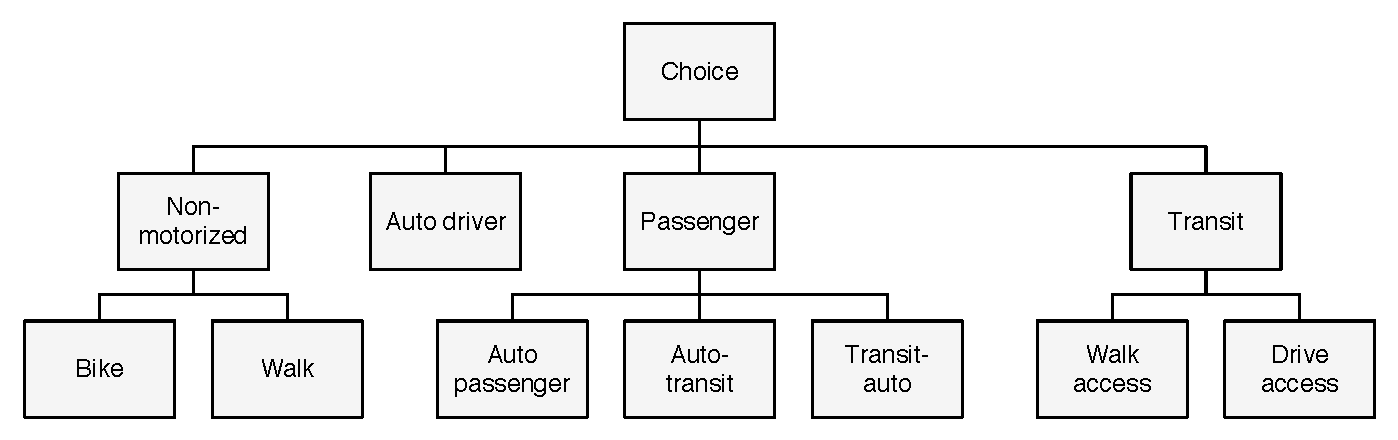
\includegraphics[width=6in]{pt/nesting}
\caption{Tour mode choice nesting structure}\label{fig:sdt-tour-mode-nesting}
\end{figure}

\subsection{Intermediate stop location models}
The PT SDT intermediate stop location model chooses an alpha zone location for each intermediate stop on a tour. It is a discrete choice multinomial logit model, whose utilities are a function of the following attributes:
\begin{itemize}
\item Origin and primary destination of the tour
\item Tour purpose
\item Tour mode
\item Characteristics of each alternative alpha zone location for the stop
\end{itemize}

\noindent The model is structured so that the probability of selecting a TAZ as an intermediate stop destination is inversely related to the out-of-direction travel between the tour origin and its primary destination imposed by its selection. Note this does not preclude intermediate stops to be located farther away from home than the primary destination. The amount of out-of-direction travel is the additional travel time required to reach the intermediate stop using the tour's primary mode; that is, travel time in excess of the time required to travel directly between the tour origin and primary destination. For transit tours, a generalized travel time function is used, to account for out-of-vehicle travel time, as follows:
\begin{equation}
TravelTime_{transit} = InVehicleTime + 1.5 \times FirstWaitTime + 2.5 \times TransferWaitTime + 3.0 \times WalkTime
\end{equation}

Zones that are not reachable by transit (except for the intrazonal alpha zone) are not considered as alternatives for stops on tours whose primary mode is transit.

\subsection{SDT intermediate stop duration models}\label{sec:sdt-intermediate-stop-duration}
The PT SDT intermediate stop duration models predicts the duration of intermediate stops on tours. It is a discrete choice multinomial logit model, where the choice set has a resolution of one hour and includes a total of twelve possible activity durations, ranging from 0-1 hour, 1-2 hours, etc., up to 11 hours or longer. The base alternative is stop duration of one hour or less. The choice set is constrained by the total duration of the tour; that is, alternatives longer than the tour duration are not allowed. The utility function includes daily activity pattern, traveler, and stop attributes. 

\subsection{SDT trip mode choice model}\label{sec:sdt-trip-mode-choice}
The trip mode choice model predicts trip mode, contingent on the previously determined tour mode. The choice set for each trip is determined by the tour mode, as previously shown in Table \ref{tab:sdt-allowable-modes}, and summarized as:
\begin{itemize}
\item If the tour mode is walk, all trips on the tour are walk trips.
\item If the tour mode is bike, all trips on the tour are bike trips.
\item If the tour mode is auto driver, the available trip mode choices are drive-alone, shared ride 2 and shared ride 3+.
\item If the tour mode is auto passenger or the auto passenger leg of a passenger/transit tour, the available trip mode choices are shared ride 2, shared ride 3+ and walk.
\item If the tour mode is walk access transit or the transit leg of a passenger/transit tour, the available trip mode choices are walk to transit and walk. The transit assignment selects the best transit path for this trip.
\item If the tour mode is drive access transit, the first and last trips on the tour are drive to transit trips; other trips are passed to the transit path builder to determine whether the trip mode is walk to transit or walk.
\end{itemize}

Where the trip mode is not uniquely defined by the tour mode nor determined by the transit path builder, the model uses a multinomial discrete choice logit model, with the following attributes:
\begin{itemize}
\item Level of service (in vehicle time, operating cost including parking costs)
\item Household attributes (e.g., household size and income)
\item Alternative specific constants,stratified by tour mode
\end{itemize}

\subsection{SDT work-based activity duration model}
This model forecasts the duration of the three activities that comprise a work based subtour:
\begin{itemize}
\item First at-work activity
\item Primary activity
\item Last at-work activity
\end{itemize} 

\noindent The duration of each individual activity is determined by applying Monte Carlo sampling from a set of empirical distribution functions based on Home Interview data. Two functions describing activity durations were calculated: the proportion of the total tour duration spent at the primary activity and the proportion of the total work activity spent at the first at-work activity. Each of these is described below.

The duration of the primary activity of the work-based subtour is constrained by the total duration of the tour, as follows:
\begin{equation}
PctDuration_{primary} = Duration_{primary} / Duration_{tour}
\end{equation}

\noindent The duration of the first at-work activity duration is constrained by the total duration of the work activity, as follows:
\begin{equation}
PctDuration_{first at-work} = Duration_{first at-work} / Duration_{work}
\end{equation}

\noindent PT SDT samples from the frequency tables to obtain the percent duration of the primary and first at-work activities. Given that the duration of the tour is known (exclusive of intermediate stop durations, if present), then the primary and first-at work durations are obtained by solving the equations above and the second at-work duration is obtained as:
\begin{equation}
Duration_{second at-work} = Duration_{tour} - Duration_{primary} - Duration_{first at-work}
\end{equation}

\subsection{LDT tour pattern model}\label{sec:ldt-tour-pattern}
Given the initial LDT long-term choice of travel (LDT rather than SDT, see \S\ref{sec:sdt-aggregate-accessibilities}), LDT next determines if travel occurs on the simulation day and if so what type. The five possible patterns of long distance travel were defined previously in Table \ref{tab:ldt-trip-purposes}. The decision-making agent for household travel is the household and the decision making agent for work-related and other travel purposes is the person.

Because so few travelers take more than one long-distance tour in a single day (one percent in the Ohio long-distance surveys), the tour pattern model does not allow for multiple long-distance tours on the model day. It is not uncommon, however, for travelers to make multiple long-distance tours during the two-week travel window (see \S\ref{sec:sdt-aggregate-accessibilities}), making it more likely that some travel will occur on the model day. Travelers making multiple long-distance tours were included when the tour pattern choice frequencies were developed, such that they implicitly reflect this scenario.

Since the long-distance travel model predicts behavior on a typical weekday, Monday through Thursday, there are no explanatory variables to logically sample among different ``typical weekdays''. Thus, the LDT tour pattern model draws from the observed frequency of each pattern type from along distance travel survey.

\subsection{LDT scheduling model}
LDT tours are scheduled to a time-of-day with a one-hour resolution. Beginning tours are given a departure time, ending tours are given an arrival time and complete tours are given a departure time and duration to fully define their schedule. As with the tour pattern model, the scheduling model draws from observed frequency distributions found in a long distance travel survey.

For complete tours, the schedule is determined using a constants-only logit model, with constants on the departure time and duration. This strategy was applied to smooth the outcomes because observed data was found to have high unexplained variability when viewed in both dimensions.

\subsection{LDT internal-external choice model}\label{sec:ldt-internal-external}
The LDT internal-external choice model is a binary choice model predicting whether a tour will have a destination within the model area or beyond the bounds of the model area. All model coefficients are applied to the utility of leaving the model area. The linear utility function contains the following variables:
\begin{itemize}
\item Household attributes (i.e., income)
\item Person attributes (i.e., occupation, worker binary, age)
\item Complete travel in one day
\item Auto travel time to external station
\item Constant
\end{itemize}

\subsection{LDT destination choice model}
The LDT destination choice models are applied separately for internal versus external destinations. The internal destination choice uses a logit model with utility variables, as specified below:
\begin{itemize}
\item Mode choice logsum
\item Auto travel time (if complete travel in one day)
\item Various size terms (i.e., households, employees, hotel employment, higher education employment, government employment, employment in worker's own industry)
\item Distance flags
\end{itemize}

LDT external destinations cannot be modeled in the same way as internal destination because detailed level-of-service and socioeconomic information are not available outside the model area. Because SWIM2 does not maintain a national network and associated extensive external zone system to associate detailed trip origins and destination, SWIM2 trips are assigned to the selected set of external stations at the edge of the model area (zones numbered in 5000s). Trips are then distributed to the external stations using a simple logit destination choice model with the following utility variables:
\begin{itemize}
\item Highway travel time (as impedance)
\item Traffic volumes at the station (as the size term)
\end{itemize}

\subsection{LDT mode choice model}
The LDT mode choice models include four alternatives in the base year and two optional future year transit options, as shown in Figure \ref{fig:mode-choice-model-nesting-structure}. The base year transit alternatives include walk-to-transit and drive-to-transit alternatives, which cover the existing intercity Greyhound. Amtrak intercity rail service is a separate choice from high-speed rail. The internal model choice model uses a nested logit equation with the following utility variables:
\begin{itemize}
\item Travel/wait time for each trip segment
\item Travel cost as a function of household income
\item Transit nesting coefficients
\item Modal constants
\end{itemize} 

\noindent As with other LDT modules, a simplified mode choice model is applied for trips with destinations outside the model area. In this case, fixed mode splits are applied.

\begin{figure}  % Figure 7.4 Mode Choice Model Nesting Structure
\centering
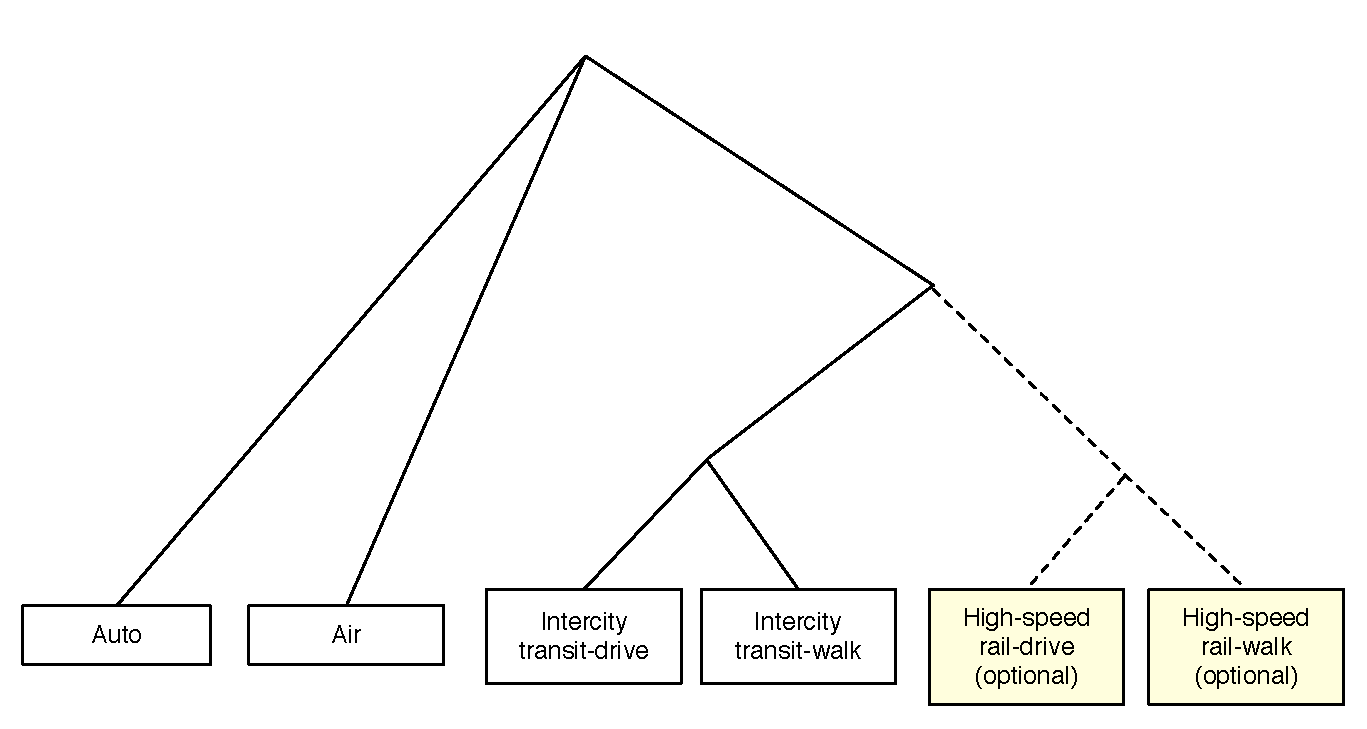
\includegraphics[width=5.5in]{pt/mode-choice-model-nesting-structure}
\caption{LDT mode choice model nesting structure}
\label{fig:mode-choice-model-nesting-structure}
\end{figure}
 
\subsection{Integration}
PT mode choice and destination choice logsums are created at the alpha zone level in compressed zip matrix format. Once PT produces skims at the alpha zone level, it also performs a ``squeeze'' function to produce selected logsum skims at the more disaggregate beta zone level for use in AA. This function will be set to average the component alpha zone values in each beta zone. A weighted average using trip ends will be used once PT is calibrated.

\section{Software implementation}
PT is implemented in the Java programming language, run in a distributed environment across a cluster of computers in order to reduce run times. The model is run in a sequence of steps:
\begin{itemize}
\item Create aggregate mode choice logsums matrices.
\item Create aggregate destination choice logsums matrices.
\item Run auto ownership model for all households.
\item Run workplace location model for all employed persons.
\item Generate a daily pattern of activities for each person by choosing an activity pattern. Each activity implies a nominal location and sequence of activities. Three models are applied to fully specify the day pattern: the generalized pattern model, the stop pattern choice model and the stop purpose model.
\item For each tour in the pattern for each person:
\begin{itemize}
\item Choose the tour schedule: the tour scheduling model for the appropriate tour purpose is applied to select the tour home departure time and the tour duration.
\item Choose a primary destination for the tour: do not choose a destination for work if a location has already been determined in the workplace location model. The tour primary destination choice model for the appropriate tour primary activity is applied to choose a location alpha zone.
\item Choose a primary mode for the tour.
\item Choose a location for each intermediate stop on the tour. The intermediate stop location is a function of the tour primary mode and the location of the tour origin and primary destination.
\item Choose a duration for each intermediate stop on the tour.
\item Choose a trip mode if the tour primary mode is not transit nor the transit leg of a transit-passenger or passenger-transit tour.
\end{itemize}
\item If the tour includes work-based subtours, then for each subtour:
\begin{itemize}
\item Calculate the durations of the three activities that make up the work-based tour, conditional on the duration of the work activity.
\item Calculate the percent of time at the primary destination of the tour
\item Calculate the percent of the at-work portion of the total tour duration that is the first at-work activity.
\item Calculate the duration of the three subtour activities.
\end{itemize}
\end{itemize}

\subsection{PT distributed processing}
Because of the computational requirements of the PT module to micro-simulate a full weekday of activities and travel for several million people within the model area, PT was built to run on a distributed application framework (DAF). The PT-DAF software implementation consists of the following tasks:
\begin{itemize}
\item PTMasterTask
\item MCLogsumCalculatorTask
\item DCLogsumCalculatorTask
\item WorkplaceLocationWorkerTask
\item MicroSimulationWorkerTask
\item LongDistanceTask 
\item Several file writer tasks  
\end{itemize}

\noindent The PTMasterTask, the LongDistanceTask, and the file writer tasks each occupy their own node while the remaining five nodes each have an MC and a DCLogusmCalculator task and multiple MicroSimulationWorkerTasks running on them. 

The PTMasterTask first instructs the MCLogsumCalculatorTasks to calculate a matrix of aggregate mode choice logsums. Although the full mode choice model is applied later, PT pre-calculates an aggregate set of mode choice logsums, which only depend on the activity purpose and market segment. The PTMasterTask sends an activity purpose (Table \ref{tab:sdt-tour-def}) and a market segment (Table \ref{tab:sdt-market-segments}) to each CalculatorTask. The CalculatorTask calculates the logsums for each alpha zone and stores the values in a matrix. The matrices are then passed to the MCWriterTask, which writes the mode choice logsums out to disk in compressed matrix format (Figure \ref{fig:daf-process}) for use later by PT (alpha zone) as well as by the AA module (beta zone). 

\begin{figure}
\centering
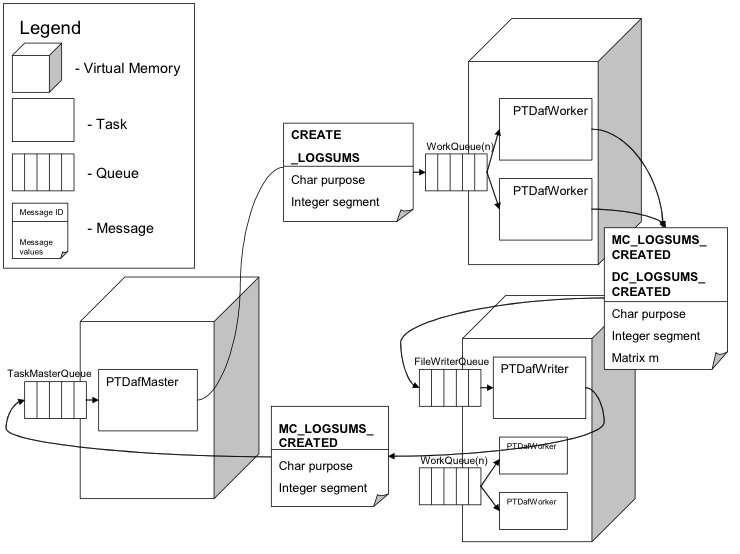
\includegraphics[width=5.2in]{pt/figure75}
\caption{DAF process to create mode choice logsums}
\label{fig:daf-process}
\end{figure}

Next the MasterTask assigns each MicroSimulationWorkerTask a set of households to apply the AutoOwnership model to. The full set of households is divided evenly amongst the set of worker tasks. The results are returned to the MasterTask via an array indexed by household ID number. 

Once all the households have been processed, the full array of auto-ownership results is sent back to the Workers so that it can be used in the workplace location model. For this model, the MasterTask assigns each MicroSimulationWorkerTask a set of persons to apply the workplace location model to. The results are sent back to the MasterTask as a mapping between the hhId\_personId (key) and the workplace TAZ (value), as shown in Figure \ref{fig:daf-workplace}. In addition, each worker task sends back a summary of its person's employment by occupation by zone to the MasterTask, where it is tabulated and written to disk as Employment.csv. 

% What was formerly Figure 7.5 doesn't appear to be referenced in the text, so
% we'll pull it from the paper
%\begin{figure}
%\centering
%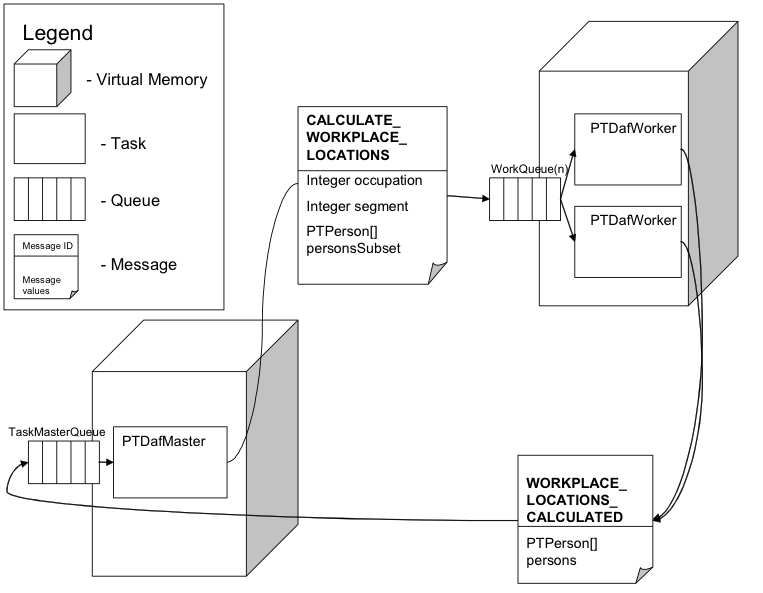
\includegraphics[width=5.2in]{pt/figure76}
%\caption{DAF process to calculate workplace locations}
%\label{fig:daf-workplace}
%\end{figure}

After the workplace location model is finished, the destination choice logsums can be calculated. The work is divided up into nine segments so that each DCLogsumCalculatorTask does at least one segment. Before beginning the calculation, each CalculatorTask reads in the latest Employment.csv file and updates their TAZ objects that are used in the size term calculations. The results are sent to the DCWriterTask which creates a table and when the work is completed is written out to disk to be used in future calculations [dclogsums.csv]. 

Once the destination choice logsums are complete, the MasterTask again divides the households evenly amongst the MicroSimulationWorkerTask so the remaining models can be applied. The first set of models in the sequence relate to the long-distance models. Each household decides if the entire household or specific members of the household will make a long distance tour on the model day (long-distance binary choice and long distance pattern choice model). If long-distance tours do occur, Tour objects are formed and sent to the LongDistanceWorkerTask for processing (see LongDistanceWorkerTask description below). The next set of models applied relate to the short-distance travel models. For each household (that does not make a long-distance tour), then for each person (that does not make a long-distance tour), the workers execute the day pattern model, calculating the weekday pattern that determines the person's weekday tours. The workers then loop through each tour and calculate the activity duration, the tour primary destination, tour primary mode choice, intermediate stop destinations, trip mode choice and secondary work-based tour characteristics (duration, destination and mode). 

Once all the members of a household have been processed the worker task sends the Household object (that now contains Person objects that contain Tour objects) to the PTResultsWriterTask where a sequence of files are written to. The outputs written include a Household file [HouseholdData.csv], a Pattern file [WeekdayPattern.csv], a Tour file [WeekdayTour.csv] and most importantly a Trip file [weekdayTrip.csv]. The Trip file is used by VISUM to compile trip matrices by time period for assignment to the network. 

The Long-DistanceWorkerTask applies all of the long-distance models to the tours that were produced by the earlier binary choice models. This includes the scheduling model, the internal/external model, the internal mode and destination choice models, the external mode and destination choice models and the auto details model. Once the tours have been processed, the results are sent to the PTResultsWriterTask which adds the results to LDT specific output files. These include a PersonTour file [ldTours.csv] and a PersonTrips file [ldTrips.csv]. The trips file is used by VISUM in the assignment procedure.

\section{S1 and S2 Module Parameters}\label{sec:pt-s1-s2}
The PT module requires a series of parameters, discussed below by sub-module. Many of the SDT utility function coefficients were originally estimated with the 1995/2000 Ohio Household Survey data, using maximum likelihood methods. In cases, particularly in LDT where the data are unavailable, explanatory variables are insignificant or budget constraints limit analysis, the model components draw from static frequency distributions. LDT estimation was also based on the Ohio Long Distance Travel Survey. These SDT and LDT parameters were adopted in Oregon, adjusting only the utility constants during calibration to Oregon-specific data. In later stages of calibration, mode choice and destination log sums are updated and downstream parameters recalibrated iteratively, until minimal change occurs in this cycle.

Ohio Travel behavior data for the estimation and calibration of the PT SDT models, later transferred to Oregon, were obtained from four home interview surveys and from the 2000 Census. The SWIM2 PT module utility constants were adjusted to match Oregon data:
\begin{itemize}
\item The Ohio Statewide Home Interview Survey, conducted in 2002
\item The OKI Regional Council Home Interview Survey, conducted in 1995
\item The MORPC Home Interview Survey, conducted in 1995
\item The NOACA Home Interview Survey, conducted in 1994
\item 2000 Census Transportation Planning Package
\end{itemize}

\noindent These four surveys comprise a total sample of 26,200 households. The OKI, MORPC and NOACA surveys were re-weighted and re-expanded using Census 2000 data. The surveys were processed to eliminate missing or illogical information, as well as to conform to a unique coding scheme of household, person and trip/activity attributes.

LDT parameter estimation was done for the 2000 Ohio statewide model using the 2002-2003 Ohio Long distance travel survey. These LDT parameters were adopted in Oregon, adjusting only the utility constants during calibration to Oregon-specific data.

\subsection{SDT aggregate accessibilities model estimation}
The aggregate accessibilities used for ``feed-up'' of lower level models to upper level models are mode choice logsums and destination choice logsums. Mode choice logsums are the natural log of the denominator of the mode choice model, which is equivalent to a composite utility of travel across all modes of transportation, weighted by the probability of selection of each mode. Mode choice logsums are created for each household segment and tour purpose and are stored in matrices by origin and destination alpha zone. Destination choice logsums are the natural log of the denominator of the destination choice model, which is equivalent to a composite utility of accessibility across all possible destination zones, weighted by the probability of selection for each TAZ. Since the destination choice model relies on mode choice logsums as the measure of accessibility, the accessibility is based on a consideration of all modes of travel to each zone. Parameters used to produce the PT SDT aggregate accessibilities are the same as those used in the disaggregate SDT tour primary destination choice and tour mode choice components (see Sections \ref{sec:sdt-primary-tour-scheduling} and \ref{sec:sdt-intermediate-stop-location}, respectively). However, since the aggregate accessibilities are pre-computed, certain situational variables, such as number of stops on tour, are not available and are ``turned off'' when computing aggregate accessibilities for upper level components.

\subsection{LDT binary choice of travel model estimation}
The LDT binary choice of travel model predicts if a person will engage in any long distance travel of each purpose during a two-week period. All model coefficients are applied to the utility of traveling. The coefficients were calibrated to match targets for each purpose derived from the Ohio Statewide survey data, but scaled to match total trips from the Oregon element of the 1995 American Travel Survey \citep{bts97}, as shown in Table \ref{tab:ldt-binary-choice-parameters}. The significant descriptive variables are primarily demographic characteristics. Households with more workers and larger households are less likely to travel probably because there are more family ties keeping them home. Households with more autos and higher incomes are more likely to travel due to a higher mobility level and a greater ability to absorb the cost. Certain occupations are more or less likely to travel long-distances, as would be expected. Men are more likely to go on business trips, probably because they tend to have fewer child-care responsibilities. As the short-distance destination choice logsum coefficients indicate, long-distance travel is less necessary if there are more attractive destinations within 50 miles. Finally, individuals who travel with their entire household are less likely to travel on their own. 

\begin{table}[!t]  % 7 8
\centering
\caption{LDT binary choice of travel model parameters}\label{tab:ldt-binary-choice-parameters}
\small
\begin{tabular}{lrrr}
\hline
 & Household & Work-related & Other \\
Variable & coefficients & coefficients & coefficients \\
\hline
Constant & -1.14618 & -6.61398 & -2.06888 \\
\gray Household workers = 1 & -0.3364 &  &  \\
Household workers = 2 & -0.3476 & -0.2928 &  \\
\gray Household workers = 3+ & -1.1494 & -0.3462 &  \\
Household autos = 1 &  &  & 0.419 \\
\gray Household autos = 2 &  &  & 0.606 \\
Household autos = 3+ &  &  & 0.846 \\
\gray Household size = 2 &  &  & -1.149 \\
Household size = 3 & -1.1637 &  & -0.898 \\
\gray Household size = 4+ & -1.4137 &  & -0.809 \\
Household income = \$20-40K & 0.387 &  & 0.289 \\
\gray Household income = \$40-60K & 0.746 &  & 0.417 \\
Household income = \$60K+ & 1.248 & 0.581 & 0.695 \\
\gray Single family dwelling household & 0.254 &  & -0.161 \\
Students = 3+ &  & 0.276 &  \\
\gray Occupation = Agriculture/farming/mining &  &  & -0.636 \\
Occupation = Manufacturing & -0.297 & -0.430 & -0.474 \\
\gray Occupation = Transportation & -0.366 &  & -0.372 \\
Occupation = Wholesale &  & 0.884 &  \\
\gray Occupation = Finance &  & 0.778 &  \\
Occupation = Other services & -0.181 &  & -0.101 \\
\gray Occupation = Professional & -0.3169 &  & -0.1601 \\
College student & -0.242 &  & 0.455 \\
\gray Male &  & 0.806 &  \\
Age &  & 0.100 & 0.051 \\
\gray Age squared &  & -0.001 & -0.001 \\
Short distance destination choice logsum & -0.182 &  & -0.119 \\
\gray Household long distance tour &  & -0.842 & -0.324 \\
\hline
\end{tabular}
\end{table}

\subsection{SDT auto ownership model estimation}
The final estimated SDT auto ownership model discussed in \S\ref{sec:sdt-auto-ownership} is shown in Table \ref{tab:sdt-auto-ownership-parameters}. All variables have significant and logical coefficients. The likelihood of higher auto ownership increases with household size, income, and employed household members. Higher auto ownership decreases with increasing destination choice logsum, meaning that households tend to own fewer cars when they are located near places with high employment. In the destination choice logsum calculation of equation \ref{eq:7.1} the distance coefficient is -0.01835 and the time coefficient is -0.025, parameters $a$ and $b$ in the equation.

\begin{table}   % 7 9
\centering
\caption{SDT auto ownership model parameters}\label{tab:sdt-auto-ownership-parameters}
\small
\begin{tabular}{lrr c rr c rr}
\hline
 & \multicolumn{8}{c}{\textit{Choice alternatives}} \\
 & \multicolumn{2}{c}{One auto} & & \multicolumn{2}{c}{Two autos} &  & \multicolumn{2}{c}{Three+ autos} \\
\cline{2-3}\cline{5-6}\cline{8-9}
Variable & Coefficient & t statistic &  & Coefficient & t statistic &  & Coefficient & t statistic \\
\hline
2 person household & 0.473 & 5.3 &  & 2.845 & 29.8 &  & 2.611 & 23.2 \\
\gray 3+ person household &  &  &  & 2.523 & 44.7 &  & 2.868 & 35.3 \\
Household income = \$20-40K & 1.281 & 15.9 &  & 2.002 & 22.1 &  & 2.225 & 19.2 \\
\gray Household income = \$40-60K & 1.576 & 12.5 &  & 2.995 & 22.7 &  & 3.519 & 23.6 \\
Household income = \$60K+ & 1.658 & 8.1 &  & 3.824 & 18.5 &  & 4.549 & 20.9 \\
\gray 1 household worker & 1.068 & 13.1 &  & 1.226 & 14.0 &  & 1.530 & 15.2 \\
2 household workers & 0.501 & 3.0 &  & 1.723 & 10.3 &  & 2.204 & 12.6 \\
\gray 3+ household workers &  &  &  &  &  &  & 2.731 & 29.8 \\
Destination choice logsum & -0.423 & -6.3 &  & -0.815 & -11.3 &  & -1.280 & -16.8 \\
\gray Constant & 5.811 & 7.1 &  & 7.904 & 9.1 &  & 11.508 & 12.9 \\
\hline
Final likelihood & -21650 &  &  &  &  &  &  &  \\
Rho-squared wrt zero & 0.380 &  &  &  &  &  &  &  \\
Sample size & 25175 &  &  &  &  &  &  &  \\
\hline
\multicolumn{9}{l}{\footnotesize Note:  Estimation using Ohio statewide Home Interview survey. Constants adjusted in Oregon-specific calibration.}
\end{tabular}
\end{table}

\subsection{SDT workplace location choice model estimation}
The only parameter in the SDT workplace location choice model discussed in \S\ref{sec:sdt-workplace-location-choice} is a gravity model dispersion parameter, $\lambda$. It retains the initial value set at 0.54, which was based on a work location choice model that was previously estimated using Oregon household survey data.

\subsection{SDT day-pattern model estimation}\label{sec:pt-day-pattern-estimation}
The estimation results for the five day pattern models discussed in \S\ref{sec:sdt-day-pattern} are summarized in Table \ref{tab:pt-day-pattern-summary}. The detailed listings of variables and parameters estimates are included in Appendix \ref{app:day-pattern-models} (page \pageref{app:day-pattern-models}). 

Among the most powerful explanatory variables across all models are number of tours, presence and/or number of intermediate stops, and number of activities of each purpose. As expected, as the day pattern complexity increases, with complexity measured as either more tours, more activities or more intermediate stops on tours, the less likely the pattern is to be chosen. The models also show that people manage day pattern complexity by trading off number of intermediate stops against number of tours, as shown by the negative coefficients on the product of intermediate stops and tours (see Tables \ref{idunno} and \ref{tab:pt-nonworker-person-day-pattern}). % and the negative coefficient on the product of stops on work tours and number of non-work tours (see Table \ref{idunno}).

\begin{table}
\centering
\caption{Day pattern model calibration outcome summary by tour type}
\label{tab:pt-day-pattern-summary}
\begin{tabular}{lrrrl}
\hline
Tour type & Variables & Final likelihood & $\rho^2$ wrt zero & Detailed summary \\
\hline
Pre-school person day pattern & 53 & -11046 & 0.4274 & Table \ref{tab:pt-preschool-person-day-pattern} (page \pageref{tab:pt-preschool-person-day-pattern}) \\
\gray Grade/high school day person pattern & 56 & -27249 & 0.4702 & Table \ref{tab:pt-grade-highschool-person-day-pattern} (page \pageref{tab:pt-grade-highschool-person-day-pattern}) \\
College student day pattern & 90 & 15496 & 0.2780 & Table \ref{tab:pt-college-student-day-pattern} (page \pageref{tab:pt-college-student-day-pattern}) \\
\gray Worker day pattern & 95 & -97414 & 0.3939 & Table \ref{tab:pt-worker-day-pattern} (page \pageref{tab:pt-worker-day-pattern}) \\
Non-worker day pattern & 60 & -97414 & 0.3939 & Table \ref{tab:pt-nonworker-person-day-pattern} (page \pageref{tab:pt-nonworker-person-day-pattern}) \\
\hline
\end{tabular}
\end{table}

The tour sequence variables are also very significant. These variables explain the likelihood of engaging in shop, recreational and other activities before or after work or school, as well as the sequencing of work and school when both activities are part of the day pattern. All models show there is significantly less likelihood of making shop, recreational or other tours before either a school or work tour, with social/recreational tours being less likely to appear before work or school tours than shop tours. 

Both pre-school and grade/high school students are very unlikely to have a day pattern that includes two or more home-based school tours. Grade/high school students are more likely to make a tour that includes both school and work than separate school and work tours. When a work tour is present in their day pattern, it is more likely to appear after the school tour than before. If they self-reported being workers, these students are less likely to choose a pattern that consists of one home-based school tour with no work stops than any other pattern. The likelihood of choosing a day-pattern that includes a work activity is higher for students between 15-17 years old than for younger students. If a school tour has stops, it is most likely to be an inbound stop.

College students are very likely to have a day pattern that is either just a home-based work tour or a home-based school tour without work stops. Patterns that include both school and work tours are also more likely than staying at home, with work after school being the most likely sequence. Patterns with a tour that includes both school and work activities are also more likely than staying at home. And when the day pattern does not include school or work, it is likely to consist of three or more tours, suggesting that the most complex trip-making behavior is left for (or possible on) days that do not include long-duration mandatory activities. Similarly, tours that include both work and school activities are unlikely to have additional stops on it, suggesting limited ability to engage in non-mandatory activities. Outbound stops on work or school tours are very unlikely, while work and school tours with both inbound and outbound stops are more likely than tours with no stops or with only inbound or outbound stops. The same behavior is observed for patterns that include both work and school.

For workers, the most likely pattern consists of a single home-based work tour (no stops) followed by a pattern that includes one work tour (no stops) among other tours. If there are stops on the work tours, inbound stops are more likely than outbound stops. Work-based tours are relatively rare; work-based tours with stops are more likely than work-based tours without stops.

For non-workers the most likely pattern is to stay at home, followed by a single home-based other tour. Their day-pattern is more likely than not to include a recreation tour. When both shop and recreation tours are present in the pattern, the recreation tour is more likely to occur after the shop tour, rather than before. As observed for the other person types, tours with outbound stops are less likely than tours with inbound stops or no stops at all.

The models show multiple, significant and logical effects when the traveler components (age, gender, auto ownership, etc.) are interacted with the activity components:
\begin{itemize}
\item The oldest preschoolers are more likely to engage in out-of-home recreational activities than the youngest children.
\item The likelihood of a school tour increases with preschooler age.
\item Preschoolers are more likely to stay at home if there is a non-working adult in the household or if it is a low income household.
\item Multiple tours or stops on tours are less likely when the household is car-insufficient (owns no cars or owns less cars than adults or workers).
\item Recreational activities (tours or stops) are more likely for persons in high income households.
\item Shopping activities are more likely for persons in high income households.
\item Grade/high school students are less likely to make stops for shop, recreational or other purposes when there is a non-working adult in the household, but more likely to do so when there is only one adult in the household, suggesting sharing of household responsibilities.
\item Grade/high school students are more likely to perform shop tours if they are old enough to drive and there more cars than adults in their household.
\item Female adults are more likely than male adults to engage in shopping activities;
\item When compared against adults 18 to 25 years old, the likelihood of participating in social/recreational activities decreases with age.
\item The youngest adults (18 to 25 years old) are the most likely to stay at home, regardless of whether they are college students, workers or non-workers.
\item Adults with pre-school children at the most likely to stay at home.
\item A worker is less likely to participate in recreational activities if he/she lives in a multiple adult household or if he/she has children.
\item A worker is more likely to have shopping activities if he/she is single and has children.
\end{itemize}

The estimation results for variables that interact accessibility variables with day-pattern composition variables are also significant and logical: 
\begin{itemize}
\item For workers and college students, the likelihood of a multiple tour pattern decreases with increasing home-to-work distance.
\item For college students, the likelihood of making multiple stops on work tours decreases with home to work distance, except when the home is more than 25 miles away from work. Workers are more likely to make stops on their work tours if their home-to-work separation is more than 50 miles. Together, these two results suggest that people tend to decrease stops as their trip length increases, until they reach a distance threshold such that their only way to fulfill their activity needs/desires is by making stops (rather than by performing additional tours).
\item As the destination choice logsum increases (meaning higher accessibility), people are more likely to make more tours and less likely to make stops. They are also less likely to stay at home.
\end{itemize}

\noindent For calibration, the Day-Pattern Model parameters controlling for choice of pattern with respect to specific pattern attributes (i.e., numbers and types of activities on pattern) are considered S2 parameters, the others are S1 parameters.

\subsection{SDT stop pattern and intermediate stop pattern models estimation}
The SDT intermediate stop pattern models include distributions for identification of stop purpose for tours in 2+ tour patterns and a multinomial model for number of intermediate stops for those with 3+ tour patterns by activity type. The trip purpose distributions were derived from Oregon Home Interview Survey data, and are shown in Table \ref{tab:sdt-2t-intermediate-stop-purpose} for 2-stop tour patterns and Table \ref{tab:sdt-3t-intermediate-stop-purpose} for 3+ tour patterns. The stop purpose probabilities are based on expanded data. The distributions are conditional on person type, tour purpose, tour position (3+ tours only), tour number (2 tours only) and tour position (3+ tours only) and stop position (2 tours only). 

The estimation results for the stop choice model, estimated for each tour purpose based upon the Oregon Home Interview Survey, are shown in Table \ref{tab:pt-intermediate-stop-number-models}. It is a discrete choice multinomial logit model with four alternatives, as discussed in \S\ref{sec:sdt-stop-pattern}. Since none of the explanatory variables are alternative-specific, they were entered in the utility function with a different coefficient for each alternative; that is, there are no generic coefficients in these models. A wide range of tour and day-pattern composition variables were tried in all models; only those that resulted in significant coefficients were retained. When a coefficient was made generic across two alternatives, the t-statistic is reported only on one of the alternatives, but the coefficient is reported for both.

\begin{sidewaystable}
\centering
\caption{Two tour intermediate stop purpose model, by market segment}
\label{tab:sdt-2t-intermediate-stop-purpose}
\small
\setlength{\tabcolsep}{3pt}
\begin{tabular}{crrrcrrrcrrrcrrr|rrrcrrrcrrrcrrr}
\hline
 & \multicolumn{15}{c|}{Number of observations} & \multicolumn{15}{c}{Stop purpose probabilities} \\
\cline{2-31}
 & \multicolumn{7}{c}{Tour 1} & & \multicolumn{7}{c|}{Tour 2} & \multicolumn{7}{c}{Tour 1} & & \multicolumn{7}{c}{Tour 2} \\
\cline{2-8}\cline{10-16}\cline{17-23}\cline{25-31}
 Tour & \multicolumn{3}{c}{Outbound} & & \multicolumn{3}{c}{Inbound} & & \multicolumn{3}{c}{Outbound} & & \multicolumn{3}{c|}{Inbound} & \multicolumn{3}{c}{Outbound stops} & & \multicolumn{3}{c}{Inbound stops} & & \multicolumn{3}{c}{Outbound stops} & & \multicolumn{3}{c}{Inbound stops} \\
\cline{2-4}\cline{6-8}\cline{10-12}\cline{14-16}\cline{17-19}\cline{21-23}\cline{25-27}\cline{29-31}
purpose & S & R & O & & S & R & O & & S & R & O & & S & R & O & S & R & O & & S & R & O & & S & R & O & & S & R & O \\
\hline
\multicolumn{31}{l}{\textit{Pre-school persons}} \\ \hline
C & 1 & 5 & 26 & & 9 & 9 & 29 & & 0 & 0 & 2 & & 0 & 0 & 6 & 0.006 & 0.245 & 0.748 & & 0.172 & 0.244 & 0.584 & & 0 & 0 & 1 & & 0 & 0 & 1 \\
\gray S & 9 & 9 & 50 & & 5 & 7 & 26 & & 12 & 15 & 31 & & 3 & 8 & 23 & 0.114 & 0.097 & 0.788 & & 0.107 & 0.161 & 0.732 & & 0.211 & 0.302 & 0.487 & & 0.122 & 0.159 & 0.719 \\
R & & 2 & 15 & & & & 14 & & & 6 & 23 & & & & 22 & & 0.022 & 0.978 & & & 0 & 1 & & & 0.197 & 0.803 & & & 0 & 1 \\
\gray O & & & 27 & & & & 5 & & & & 25 & & & & 5 & & & 1.000 & & & & 1 & & & & 1 & & & & 1 \\
\hline
\multicolumn{31}{l}{\textit{Grade/high school persons}} \\ \hline
W & 0 & 0 & 0 & & 0 & 0 & 0 & & 0 & 1 & 2 & & 1 & 1 & 6 & 0 & 0 & 0 & & 0 & 0 & 0 & & 0 & 0.831 & 0.169 & & 0.046 & 0.073 & 0.881 \\
\gray B & 0 & 0 & 0 & & 0 & 0 & 0 & & 0 & 0 & 0 & & 0 & 0 & 0 & 0 & 0 & 0 & & 0 & 0 & 0 & & 0 & 0 & 0 & & 0 & 0 & 0 \\
C & 7 & 33 & 162 & & 22 & 110 & 209 & & 0 & 3 & 7 & & 4 & 5 & 15 & 0.022 & 0.177 & 0.802 & & 0.051 & 0.334 & 0.615 & & 0 & 0.172 & 0.828 & & 0.084 & 0.247 & 0.669 \\
\gray S & 8 & 7 & 18 & & 3 & 3 & 13 & & 26 & 73 & 87 & & 10 & 33 & 74 & 0.309 & 0.277 & 0.414 & & 0.118 & 0.294 & 0.588 & & 0.115 & 0.371 & 0.515 & & 0.066 & 0.261 & 0.673 \\
R & & 3 & 6 & & & 1 & 12 & & & 47 & 97 & & & 6 & 143 & & 0.144 & 0.856 & & & 0.039 & 0.961 & & & 0.3 & 0.7 & & & 0.051 & 0.949 \\
\gray O & & & 14 & & & & 3 & & & & 57 & & & & 10 & & & 1 & & & & 1 & & & & 1 & & & & 1 \\
\hline
\multicolumn{31}{l}{\textit{College persons}} \\ \hline
W & 5 & 1 & 31 & & 10 & 5 & 42 & & 1 & 3 & 13 & & 5 & 6 & 17 & 0.138 & 0.017 & 0.845 & & 0.11 & 0.174 & 0.715 & & 0.114 & 0.267 & 0.619 & & 0.244 & 0.221 & 0.534 \\
\gray B & 4 & 0 & 4 & & 1 & 2 & 7 & & 0 & 1 & 0 & & 0 & 0 & 2 & 0.334 & 0 & 0.666 & & 0.045 & 0.095 & 0.86 & & 0 & 1 & 1 & & 0 & 0 & 1 \\
C & 0 & 5 & 52 & & 34 & 10 & 69 & & 5 & 2 & 11 & & 9 & 13 & 21 & 0 & 0.049 & 0.951 & & 0.262 & 0.05 & 0.688 & & 0.165 & 0.235 & 0.601 & & 0.226 & 0.225 & 0.549 \\
\gray S & 11 & 5 & 24 & & 3 & 2 & 22 & & 8 & 10 & 35 & & 3 & 16 & 24 & 0.277 & 0.092 & 0.631 & & 0.074 & 0.044 & 0.882 & & 0.128 & 0.178 & 0.694 & & 0.037 & 0.343 & 0.619 \\
R & & & 10 & & & & 9 & & & 17 & 34 & & & 2 & 30 & & 0 & 1 & & & 0 & 1 & & & 0.253 & 0.747 & & & 0.091 & 0.909 \\
\gray O & & & 16 & & & & 3 & & & & 39 & & & & 6 & & & 1 & & & & 1 & & & & 1 & & & & 1 \\
\hline
\multicolumn{31}{l}{\textit{Workers}} \\ \hline
W & 65 & 26 & 589 & & 202 & 91 & 720 & & 26 & 12 & 113 & & 55 & 29 & 136 & 0.074 & 0.038 & 0.888 & & 0.153 & 0.102 & 0.745 & & 0.17 & 0.096 & 0.734 & & 0.235 & 0.115 & 0.65 \\
\gray B & 11 & 0 & 130 & & 46 & 18 & 111 & & 3 & 1 & 7 & & 3 & 3 & 14 & 0.056 & 0.035 & 0.908 & & 0.294 & 0.08 & 0.626 & & 0.157 & 0.019 & 0.824 & & 0.095 & 0.09 & 0.815 \\
S & 51 & 28 & 287 & & 41 & 19 & 149 & & 105 & 102 & 396 & & 32 & 92 & 260 & 0.126 & 0.088 & 0.786 & & 0.167 & 0.097 & 0.736 & & 0.148 & 0.159 & 0.693 & & 0.067 & 0.251 & 0.683 \\
\gray R & & 5 & 42 & & & 4 & 39 & & & 58 & 194 & & & 7 & 191 & & 0.13 & 0.87 & & & 0.1 & 0.9 & & & 0.245 & 0.755 & & & 0.04 & 0.96 \\
O & & & 231 & & & & 60 & & & & 251 & & & & 37 & & & 1 & & & & 1 & & & & 1 & & & & 1 \\
\hline
\multicolumn{31}{l}{\textit{Non-workers}} \\ \hline
\gray S & 111 & 99 & 526 & & 62 & 36 & 266 & & 81 & 56 & 248 & & 26 & 35 & 143 & 0.149 & 0.137 & 0.713 & & 0.16 & 0.128 & 0.712 & & 0.191 & 0.177 & 0.632 & & 0.132 & 0.193 & 0.675 \\
R & & 24 & 94 & & & 4 & 87 & & & 27 & 104 & & & 6 & 120 & & 0.255 & 0.745 & & & 0.042 & 0.958 & & & 0.271 & 0.729 & & & 0.096 & 0.904 \\
\gray O & & & 231 & & & & 51 & & & & 164 & & & & 46 & & & 1 & & & & 1 & & & & 1 & & & & 1 \\
\hline
\multicolumn{31}{l}{\footnotesize Note: Trip purposes are work (W), work-based (B), school (C), shopping (S), recreation (R), and other (O)} \\
\end{tabular}
\end{sidewaystable}


  % Tables 7-15 through 7-19, now combined into single table
\begin{sidewaystable}
\centering
\caption{Three+ tour intermediate stop purpose model, by market segment}
\label{tab:sdt-3t-intermediate-stop-purpose}
\small
\setlength{\tabcolsep}{4pt}
\begin{tabular}{crrrcrrrcrrr|rrrcrrrcrrr}
\hline
 & \multicolumn{11}{c|}{Number of observations} & \multicolumn{11}{c}{Stop purpose probabilities} \\
\cline{2-23}
 & \multicolumn{3}{c}{First tour} & & \multicolumn{3}{c}{Middle tour} & & \multicolumn{3}{c|}{Last tour} & \multicolumn{3}{c}{First tour} & & \multicolumn{3}{c}{Middle tour} & & \multicolumn{3}{c}{Last tour} \\
Tour & \multicolumn{3}{c}{stop purpose} & & \multicolumn{3}{c}{stop purpose} & & \multicolumn{3}{c|}{stop purpose} & \multicolumn{3}{c}{stop purpose} & & \multicolumn{3}{c}{stop purpose} & & \multicolumn{3}{c}{stop purpose} \\
\cline{2-4}\cline{6-8}\cline{10-12}\cline{13-15}\cline{17-19}\cline{21-23}
purpose & ~~S & ~~R & O & & ~~S & ~~R & O & & ~~S & ~~R & O & S & R & O & & S & R & O & & S & R & O \\
\hline
\multicolumn{23}{l}{\textit{Student person types}} \\ \hline
W &  &  &  &  & 1 & 2 & 9 &  & 4 & 6 & 46 &  &  &  &  & 0.3 & 0.085 & 0.615 &  & 0.078 & 0.083 & 0.84 \\
\gray B &  &  &  &  & 0 & 0 & 0 &  & 0 & 0 & 3 &  &  &  &  & 0 & 0 & 0 &  & 0 & 0 & 1 \\
C & 2 & 5 & 12 &  & 9 & 18 & 78 &  & 18 & 14 & 77 & 0.065 & 0.088 & 0.847 &  & 0.065 & 0.12 & 0.815 &  & 0.141 & 0.121 & 0.737 \\
\gray S & 14 & 8 & 86 &  & 19 & 25 & 104 &  & 19 & 16 & 75 & 0.139 & 0.122 & 0.739 &  & 0.063 & 0.167 & 0.77 &  & 0.129 & 0.178 & 0.692 \\
R &  & 2 & 30 &  &  & 10 & 70 &  &  & 11 & 58 &  & 0.029 & 0.971 &  &  & 0.227 & 0.773 &  &  & 0.154 & 0.846 \\
\gray O &  &  & 45 &  &  &  & 55 &  &  &  & 64 &  &  & 1 &  &  &  & 1 &  &  &  & 1 \\
\hline
\multicolumn{23}{l}{\textit{Workers}} \\ \hline
W & 67 & 24 & 328 &  & 44 & 21 & 207 &  & 9 & 5 & 40 & 0.171 & 0.061 & 0.768 &  & 0.132 & 0.057 & 0.81 &  & 0.076 & 0.122 & 0.802 \\
\gray B & 12 & 1 & 42 &  & 2 & 0 & 14 &  & 0 & 0 & 0 & 0.205 & 0.051 & 0.744 &  & 0.058 & 0 & 0.942 &  & 0 & 0 & 0 \\
S & 18 & 19 & 158 &  & 52 & 38 & 283 &  & 35 & 55 & 170 & 0.081 & 0.086 & 0.834 &  & 0.087 & 0.104 & 0.809 &  & 0.181 & 0.178 & 0.641 \\
\gray R &  & 2 & 43 &  &  & 7 & 80 &  &  & 20 & 140 &  & 0.046 & 0.954 &  &  & 0.079 & 0.921 &  &  & 0.079 & 0.921 \\
O &  &  & 121 &  &  &  & 175 &  &  &  & 100 &  &  & 1 &  &  &  & 1 &  &  &  & 1 \\
\hline
\multicolumn{23}{l}{\textit{Non-workers}} \\ \hline
S & 52 & 29 & 257 &  & 57 & 67 & 318 &  & 27 & 33 & 127 & 0.139 & 0.082 & 0.779 &  & 0.113 & 0.172 & 0.715 &  & 0.165 & 0.137 & 0.698 \\
\gray R &  & 5 & 75 &  &  & 5 & 82 &  &  & 10 & 94 &  & 0.062 & 0.938 &  &  & 0.052 & 0.948 &  &  & 0.186 & 0.814 \\
O &  &  & 120 &  &  &  & 156 &  &  &  & 73 &  &  & 1 &  &  &  & 1 &  &  &  & 1 \\
\hline
\multicolumn{23}{l}{\footnotesize Note: Trip purposes are work (W), work-based (B), school (C), shopping (S), recreation (R), and other (O)} \\
\end{tabular}
\end{sidewaystable}


  % Tables 7-20 through 7-22, now combined into single table

% Had to move table definition to after next paragraph to get it to span two
% instead of three pages, but will probably need to re-adjust with all tables

\subsection{SDT primary tour destination choice model estimation}
The estimation results for the SDT tour primary destination choice model discussed in \S\ref{sec:sdt-primary-tour-destination-choice}, including utility expression of equation \ref{eq:7.5}, are shown in Table \ref{tab:pt-primary-destination-choice-models}. All models were estimated using either time and mode choice logsum or distance and mode choice logsums; the latter specification resulted in more logical estimates. The coefficient estimated on the mode choice logsum can be interpreted as a nesting coefficient. Thus the coefficient must range be between zero and one. A value of 1.0 implies that there is no nesting. A value greater than 1.0 implies that the nesting order is incorrect. Logsum coefficients higher than 1.0 in estimation were assigned a value lower than 1.0. The distance variable was stratified by number of tours on the day pattern and by number of stops on tours. The results show that distance decreases with the number of tours, but increases with the number of stops on the tour.

{\setlength{\tabcolsep}{4pt}
\begin{small}
\begin{longtable}{llrrrrrr}
\caption{\normalsize{Intermediate stop number models by tour type}}\vspace{-9pt} \\
\hline 
& & \multicolumn{6}{c}{Choice alternatives}	\\ \cline{3-8}
& & \multicolumn{2}{c}{Outbound} & \multicolumn{2}{c}{Inbound} & \multicolumn{2}{c}{Both} \\
Tour type & Tour stop variable & Coefficient & t statistic & Coefficient & t statistic & Coefficient & t statistic \\ \hline
\endfirsthead
\hline
& & \multicolumn{6}{c}{Choice alternatives}	\\ \cline{3-8}
& & \multicolumn{2}{c}{Outbound} & \multicolumn{2}{c}{Inbound} & \multicolumn{2}{c}{Both} \\
Tour type & Tour stop variable & Coefficient & t statistic & Coefficient & t statistic & Coefficient & t statistic \\ \hline
\endhead
\hline \multicolumn{8}{r}{\emph{Continued on next page}}
\endfoot
\hline
\endlastfoot\label{tab:pt-intermediate-stop-number-models}
Work & Work-based tour dummy & 0.400 & 3.2 &  &  & 0.406 & 2.8 \\
\gray \cellcolor{white} & First work tour in day pattern &  &  & 0.386 & 3.2 & 0.386 &  \\
 & Presence of children$<$5 yrs old & 0.922 & 5.5 &  &  & 0.936 & 4.7 \\
\gray \cellcolor{white} & Presence of children 5-15 yrs old & 0.609 & 4.4 & 0.171 & 1.6 & 0.837 & 5.4 \\
 & Grade/high school person type & -0.342 & -0.9 & -0.342 &  & -1.280 &  \\
\gray \cellcolor{white} & College person type & -0.584 & -2.1 & -0.579 & -2.8 &  &  \\
 & Constant & -2.601 & -19.9 & -1.235 & -12.5 & -2.348 & -18.3 \\ \cline{2-8}
 & Final Likelihood & -2970.931 &  &  &  &  &  \\
 & Rho-Squred wrt Zero & 0.240 &  &  &  &  &  \\
 & Sample Size & 2818 &  &  &  &  &  \\
\hline
School & Four+ tours in day pattern &  &  & -0.481 & -1.6 & -1.076 & -1.4 \\
\gray \cellcolor{white} & First school tour in day pattern & 0.856 & 1.6 &  &  & 1.961 & 1.9 \\
 & Presence of shop tours  &  &  &  &  & -0.820 & -1.8 \\
\gray \cellcolor{white} & Pre-school person type  &  &  & 0.705 & 2.1 & 0.705 &  \\
 & College person type  & 0.890 & 2.9 & 0.728 & 3.6 & 0.788 & 2.2 \\
\gray \cellcolor{white} & Constant & 5.000 & -6.6 & -1.200 & -12.8 & -3.643 & -4.6 \\
\cline{2-8}
 & Final Likelihood & -650.000 &  &  &  &  &  \\
 & Rho-Squred wrt Zero & 0.433 &  &  &  &  &  \\
 & Sample Size & 827 &  &  &  &  &  \\
\hline
Shop & Four or more tours in day pattern & -0.179 & -2.1 & -0.459 & -3.7 & -0.179 &  \\
\gray \cellcolor{white} & Presence of other shop tours & -0.137 & -1.6 &  &  & -0.442 & -3.9 \\
 & Presence of other tours &  &  & 0.251 & 2.2 &  &  \\
\gray \cellcolor{white} & Presence of work or school tours & -0.488 & -4.8 & -0.199 & -1.8 & -0.948 & -7.2 \\
 & Low income household & -0.437 & -2.8 & -0.214 & -1.4 &  &  \\
\gray \cellcolor{white} & Zero car household &  &  &  &  & -1.501 & -1.5 \\
 & Presence of children $<$15 yrs old & 0.408 & 5.0 &  &  & 0.465 & 4.3 \\
\gray \cellcolor{white} & Worker person type & 0.181 & 2.1 &  &  &  &  \\
 & Constant & -1.138 & -4.6 & -1.062 & -10.4 & -1.121 & -8.6 \\
\cline{2-8}
 & Final Likelihood & -4183.000 &  &  &  &  &  \\
 & Rho-Squred wrt Zero & 0.108 &  &  &  &  &  \\
 & Sample Size & 3382 &  &  &  &  &  \\
\hline
Social/ & Four or more tours in day pattern &  &  & -0.513 & -3.0 &  &  \\
\gray \cellcolor{white}recre- & Presence of shop tours & -0.341 & -2.7 &  &  & -0.341 &  \\
ational & Presence of other tours & 0.238 & 1.9 & -0.217 & -1.6 & 0.238 &  \\
\gray \cellcolor{white} & Presence of work or school tours & -0.556 & -3.8 & -0.323 & -2.2 & -0.510 & -2.6 \\
 & Presence of children $<$5 yrs old & 0.458 & 2.5 & 0.358 & 2.1 & 0.365 & 1.6 \\
\gray \cellcolor{white} & Preschool person type & -0.853 & -2.0 &  &  &  &  \\
 & College person type &  &  & 0.735 & 3.2 &  &  \\
\gray \cellcolor{white} & Worker person type &  &  & 0.397 & 2.6 &  &  \\
 & Constant & -1.981 & -11.8 & -1.990 & -13.7 & -3.108 & -14.5 \\
\cline{2-8}
 & Final Likelihood & -2153.000 &  &  &  &  &  \\
 & Rho-Squred wrt Zero & 0.413 &  &  &  &  &  \\
 & Sample Size & 2644 &  &  &  &  &  \\
\hline
Other & Four or more tours in day pattern &  &  &  &  & -0.778 & -3.7 \\
\gray \cellcolor{white} & Presence of shop tours &  &  &  &  & 0.596 & 1.8 \\
 & Presence of other `other' tours &  &  &  &  & 0.759 & 3.1 \\
\gray \cellcolor{white} & Presence of work or school tours & -1.044 & -7.0 & -0.970 & -6.6 & -0.929 & -4.1 \\
 & Presence of children $<$5 yrs old & 0.337 & 3.4 & 0.337 &  &  &  \\
\gray \cellcolor{white} & Presence of children 5-15 yrs old &  &  &  &  & -0.430 & -2.1 \\
 & Grade/high school person type & 0.701 & 2.4 & 0.843 & 3.4 & 0.801 & 1.8 \\
\gray \cellcolor{white} & College person type & 0.475 & 1.8 & 0.424 & 1.7 & 0.992 & 3.0 \\
 & Worker person type & 0.528 & 3.7 & 0.162 & 1.2 & 0.427 & 2.0 \\
\gray \cellcolor{white} & Constant & -2.917 & -30.9 & -1.770 & -31.5 & -3.969 & -15.8 \\
\cline{2-8}
 & Final Likelihood & -3262.000 &  &  &  &  &  \\
 & Rho-Squred wrt Zero & 0.676 &  &  &  &  &  \\
 & Sample Size & 7254 &  &  &  &  &  \\
\end{longtable}
\end{small}
}  % End of tabcolsep override
   % Tables 7-23 through 7-27, now combined
\begin{table}
\centering
\caption{Primary destination choice models by tour type}
\label{tab:pt-primary-destination-choice-models}
\small
\begin{tabular}{l *{8}{r}}
\hline
 & \multicolumn{2}{c}{College education} & & \multicolumn{2}{c}{K12 education} & & \multicolumn{2}{c}{Work-based subtours} \\
\cline{2-3}\cline{5-6}\cline{8-9}
Variable & Coefficient & t statistic & & Coefficient & t statistic & & Coefficient & t statistic \\
\hline
Distance & -0.188 & -12.1 & & -0.698 & -41.0 & & -0.198 & -1.8 \\
\gray ~~~If 2 tours & -0.027 & -2.2 & & -0.004 & -0.4 & & -0.043 & -0.4 \\
~~~If 3+ tours & -0.111 & -5.2 & & -0.068 & -2.8 & & -0.063 & -0.5 \\
\gray ~~~If stops on tour & 0.008 & 0.7 & & 0.038 & 3.6 & & & \\
~~~If preschooler & & & & & & & & \\
\gray Intrazonal indicator & -1.067 & 8.2 & & -0.544 & 31.3 & & -1.014 & 13.7 \\
Mode choice logsum & 0.443 & 4.7 & & 0.453 & 16.7 & & 0.8 (a) & \\
\gray Size terms & & & & & & & & \\
~~~Retail & & & & & & & 1.000 & \\
\gray ~~~Other services & & & & & & & 0.183 & -13.2 \\
~~~Households & & & & & & & 0.208 & -11.7 \\
\gray ~~~Health & & & & & & & 0.059 & -5.8 \\
~~~Transport \& handling & & & & & & & 0.254 & -3.0 \\
\gray ~~~Other employment & & & & & & & 0.005 & -1.9 \\
~~~High ed. employment & 1.000 & & & & & & & \\
\gray ~~~K12 ed. employment & & & & 1.000 & & & & \\
Intrarural indicator & -1.690 & & & -4.270 & & & -5.824 & \\
\hline
Rho-squared wrt zero & 0.130 & & & 0.140 & & & 0.170 & \\
Sample size & 1173 & & & 6808 & & & 2167 & \\
\hline 
\hline
 & \multicolumn{2}{c}{Shop} & & \multicolumn{2}{c}{Social/recreation} & & \multicolumn{2}{c}{Other} \\
\cline{2-3}\cline{5-6}\cline{8-9}
Variable & Coefficient & t statistic & & Coefficient & t statistic & & Coefficient & t statistic \\
\hline
Distance & -0.292 & -48.6 & & -0.197 & -44.7 & & -0.262 & -57.0 \\
\gray ~~~If 2 tours & -0.010 & -2.2 & & -0.036 & -7.0 & & -0.028 & -6.2 \\
~~~If 3+ tours & -0.040 & -6.7 & & -0.049 & -7.9 & & -0.076 & -14.8 \\
\gray ~~~If one stop on tour & 0.059 & 11.3 & & 0.043 & 8.7 & & 0.114 & 23.1 \\
~~~If two stops on tour & 0.115 & 19.1 & & 0.065 & 8.0 & & 0.169 & 20.5 \\
\gray ~~~If preschooler at home & 0.021 & 3.7 & & & & & & \\
Intrazonal indicator & -0.686 & 17.5 & & -0.249 & 24.1 & & -0.628 & 39.8 \\
\gray Mode choice logsum & 0.991 & 20.0 & & 0.76 (a) & & & 0.880 & 20.9 \\
Size terms & & & & & & & & \\
\gray ~~~Retail & 1.000 & & & 1.000 & & & 1.000 & \\
~~~Other services & 0.038 & -30.5 & & 1.755 & 2.7 & & 0.214 & -9.7 \\
\gray ~~~Households & & & & 4.616 & 8.3 & & 1.019 & 0.3 \\
~~~Government & & & & & & & 0.300 & -6.5 \\
\gray ~~~Other employment & & & & & & & & \\
Intrarural indicator & -4.697 & & & -2.515 & & & -3.474 & \\
\hline
Rho-squared wrt zero & 0.130 & & & 0.110 & & & 0.150 & \\
Sample size & 11479 & & & 8582 & & & 15621 & \\
\hline
\multicolumn{7}{l}{\footnotesize (a) Asserted coefficient}
\end{tabular}
\end{table}   % Tables 7-28 and 7-29 combined

\subsection{SDT primary tour scheduling model estimation}\label{sec:sdt-primary-tour-scheduling}
Estimation results for the SDT tour scheduling models discussed in \S\ref{sec:sdt-primary-tour-scheduling} are summarized in Table \ref{tab:sdt-scheduling-models-summary}. The detailed listing of estimated parameters and constants are shown in Appendix \ref{app:sdt-primary-tour-scheduling} (page \pageref{app:sdt-primary-tour-scheduling}), for they cover several pages. A review of those results revealed that the day pattern, traveler attribute and travel condition variables were typically interacted with both departure time shift and duration shift variables; variables were kept if they showed logical estimates for both shift variables and significant estimates for at least one of them.

\begin{table}
\centering
\caption{Summary of tour scheduling models calibration outcomes}
\label{tab:sdt-scheduling-models-summary}
\begin{tabular}{lrrrrl}
\hline
Tour type & Variables & Constants & Final likelihood & $\rho^2$ wrt zero & Detailed results \\
\hline
Work & 73 & 38 & -81685 & 0.2571 & Table \ref{tab:pt-work-tour-scheduling-model} (page \pageref{tab:pt-work-tour-scheduling-model}) \\
\gray School & 66 & 37 & -35633 & 0.3643 & Table \ref{tab:pt-school-tour-scheduling} (page \pageref{tab:pt-school-tour-scheduling}) \\
Shopping & 24 & 38 & -50945 & 0.1743 & Table \ref{tab:pt-shopping-tour-scheduling} (page \pageref{tab:pt-shopping-tour-scheduling}) \\
\gray Social and recreational & 52 & 38 & -36679 & 0.1351 & Table \ref{tab:pt-social-rec-tour-scheduling} (page \pageref{tab:pt-social-rec-tour-scheduling}) \\
\hline
\end{tabular}
\end{table}

The constant terms for all models show the expected result. Increasingly negative departure time or duration constant with decreasing observed departure time or duration frequencies. Among the day-pattern composition variables, those that describe the place of the tour in the pattern sequence relative to the length of the pattern (in tours) are very powerful and have logical signs. The departure time shifts essentially indicate that how early or late, relative to a one-tour pattern, the tour occurs. Note that a non-significant estimate simply means that the tour tends to occur at about the same time as the one-tour pattern. The duration shifts indicates that first tours tend to be the longest tours, followed by second tours, etc. This trend was observed in the data. Note as well that the duration shift variables are negative, indicating that tours in multiple tour patterns are shorter than tours in single tour patterns.

The other day pattern composition variables included in the models are dummy variables to indicate the presence of tours of a given purpose in the pattern and dummy variables to flag the presence of inbound and/or outbound stops in the tour. The models show many significant effects related to these variables, both for tour departure time and for tour duration. For example, the presence of multiple work tours in the day pattern tends to shift work tour departure times early and to shorten the duration of the tour. The presence of tours of any other purpose tends to shift the work tour departure time late and to lengthen the duration of the work tour. Note that this is after controlling for the number of tours in the pattern. The result is logical because it is essentially comparing a work tour coupled with another work tour versus a work tour coupled with a non-work tour; the work tour in the latter case is expected to be longer than the work tour in the former case. The presence of intermediate stops on the tour tends to increase the duration of the tour. However, tours with both inbound and outbound stops are on average shorter than tours with either just one inbound or just one outbound stop (one or the other, depending on purpose), suggesting that when multiple stops occur on a tour they tend to be of short duration.

The models also show multiple significant effects related to the traveler attribute variables. Among these are:
\begin{itemize}
\item Female workers tend to have later work departures and shorter work tours than male workers.
\item The youngest workers (less or equal to 25 years old) tend to have the latest work departures, while the oldest workers (55 years old or older) tend to have the shortest work tours.
\item Workers in the following industries have significantly later departure times for work than workers in all other industries:  arts \& recreation, accommodations \& food, and real estate. Workers in the latter two industries also have the shortest work tours.
\item Persons in worker households tend to make later shop tours than those in no-worker households.
\item Workers and students make longer shop tours than non-workers; women make longer shop tours than men.
\item Workers are more likely to depart late for recreation tours than non-workers or students, but students make the longest recreation tours.
\end{itemize}

The only travel condition variable estimated was tour distance, due to the unavailability of mode choice logsums when the models were estimated. The models show longer tour distance associated with earlier departure times and with longer tours. However, the structure of the models places the scheduling models before the destination choice models for all purposes other than work. Therefore the distance variable can only be used for work tours; for other tour purposes, the distance variable is set to zero. 

\subsection{SDT tour mode choice model estimation}
The SDT tour mode choice model final parameters were asserted rather than estimated in both Ohio and Oregon. An initial set of mode choice model parameters were estimated with the Oregon data. These showed reasonable and significant in-vehicle and out-of-vehicle parameters, but with implied low values of time. Also significant were the number of stops on the tour, showing a direct relationship between the number of stops and the propensity to choose auto driver. To define the final parameters asserted for these models, the in-vehicle time coefficients were set at values consistent with accepted practice, the cost coefficients were set to yield reasonable values of time and other coefficients were adjusted to exhibit similar internal relationships shown by the estimated parameters.

The final parameters are shown in Table \ref{tab:pt-tour-mode-choice-parameters}, and the constants are shown in Table \ref{tab:pt-mode-choice-constants}. All parameter values are given for the mode at the multinomial level. The auto driver mode is the base alternative for each model. Additionally, sets of descriptive statistics are provided, including the implied value of time (cost parameters are in year 2000 cents and time parameters are in minutes) and ratios of in-vehicle time to various out-of-vehicle time parameters. All models have cost parameters stratified by three household income groups.

% Table 7-35 was in two parts, with different number of columns. Thus, I've put
% them into two separate tables rather than trying to cram them into single page
\begin{table}[!t]
\centering
\caption{Tour mode choice model parameters}\label{tab:pt-tour-mode-choice-parameters}
\small
\begin{tabular}{l *{6}{r}}
\hline
Parameter & Work \& college & School & Shop & Recreate & Other & Work-based \\
\hline
In-vehicle time & -0.0250 & -0.0172 & -0.0150 & -0.0150 & -0.0150 & -0.0200 \\
{\vspace{-9pt}} \\
\textit{Cost (cents)} &  &  &  &  &  &  \\
\gray ~~~Low income ($<$\$30k) & -1.0400 & -1.0733 & -0.9360 & -0.9360 & -0.9360 & -1.2480 \\
~~~Med income ($30-$60k) & -0.2600 & -0.2683 & -0.2340 & -0.2340 & -0.2340 & -0.3120 \\
\gray ~~~High income ($>$\$60k) & -0.1300 & -0.1342 & -0.1170 & -0.1170 & -0.1170 & -0.1560 \\
{\vspace{-9pt}} \\
First wait time (2.0) & -0.0500 & -0.0344 & -0.0300 & -0.0300 & -0.0300 & -0.0400 \\
\gray Transfer wait time (2.5) & -0.0625 & -0.0430 & -0.0375 & -0.0375 & -0.0375 & -0.0500 \\
Walk time (2.5) & -0.0625 & -0.0430 & -0.0375 & -0.0375 & -0.0375 & -0.0500 \\
\gray Drive time (2.5) & -0.0625 & -0.0430 & -0.0375 & -0.0375 & -0.0375 & -0.0500 \\
Walk mode time (3.5) & -0.0875 & -0.0602 & -0.0525 & -0.0525 & -0.0525 & -0.0700 \\
\gray Bike mode time (4) & -0.1000 & -0.0688 & -0.0600 & -0.0600 & -0.0600 & -0.0800 \\
{\vspace{-9pt}} \\
\textit{Value of time} &  &  &  &  &  &  \\
~~~Low income ($<$\$30k) & 1.4423 & 0.9615 & 0.9615 & 0.9615 & 0.9615 & 0.9615 \\
\gray ~~~Med income ($30-$60k) & 5.7692 & 3.8462 & 3.8462 & 3.8462 & 3.8462 & 3.8462 \\
~~~High income ($>$\$60k) & 11.5385 & 7.6923 & 7.6923 & 7.6923 & 7.6923 & 7.6923 \\
{\vspace{-9pt}} \\
\textit{Number of stops} &  &  &  &  &  &  \\
\gray ~~~Passenger & -0.6380 & -0.3843 & -0.0867 & -0.1897 & -0.0867 & \\
~~~Walk & -1.6196 & -1.7860 & -1.2873 & -1.2962 & -1.2873 & \\
\gray ~~~Bike & -1.1752 & -1.7846 & -0.7714 & -0.8953 & -0.7714 & \\
~~~Walk-transit & -0.9393 & -0.9790 & -0.2273 & -0.6367 & -0.2273 & \\
\gray ~~~Transit-passenger & -0.1724 & -0.2749 & 0.3845 & -1.5006 & 0.3845 & \\
~~~Passenger-transit & -0.6503 & -0.2749 & 0.1511 & & 0.1511 & \\
\gray ~~~Drive-transit & -2.1832 & & & & & \\
{\vspace{-9pt}} \\
Passenger, hhsize=1 & -0.7148 & & -1.1303 & -1.1917 & -1.1303 & \\
\gray Passenger, hhsize=2 & & 0.8440 & & & & \\
Passenger, hhsize=3 & & 1.4159 & & & & \\
\gray Nesting coefficient & 0.7659 & 0.7659 & 0.7659 & 0.7659 & 0.7659 & 0.7659 \\
\hline
\end{tabular}
\end{table}  % First part (parameters)
\begin{table}[!t]  % Second half of Table 7-35 (has one more column that first half)
\centering
\caption{Tour mode choice model constants}\label{tab:pt-mode-choice-constants}
\small
\begin{tabular}{l *{7}{r}}
\hline
 & \multicolumn{7}{c}{Tour purpose} \\
\cline{2-8}
Variable & Work & School & College & Shop & Recreate & Other & Work subtour \\
\hline
Passenger & 0.0 & 0.0 & 0.0 & 0.0 & 0.0 & 0.0 & -2.51420 \\
~~~Auto$=$0 & 0.0 & 0.0 & 0.0 & 0.0 & 0.0 & 0.0 & 0.0 \\
~~~Auto$<$Workers & -0.80605 & -0.79661 & -0.12926 & -0.65097 & -0.31053 & -1.49818 & 0.0 \\
~~~Auto$\ge$Workers & -2.93411 & -4.70402 & -1.26957 & -1.54200 & -1.26270 & -1.75402 & 0.0 \\
\gray Walk & 0.0 & 0.0 & 0.0 & 0.0 & 0.0 & 0.0 & 2.60870 \\
\gray ~~~Auto$=$00 & 12.06218 & 3.33675 & 8.36162 & 3.42024 & 3.66258 & 3.04538 & 0.0 \\
\gray ~~~Auto$<$Workers & 5.14586 & 3.13756 & 5.61320 & 1.73882 & 2.24566 & 1.36735 & 0.0 \\
\gray ~~~Auto$\ge$Workers & 0.81160 & -1.23361 & 3.15801 & -0.06181 & 1.23595 & 0.19792 & 0.0 \\
Bike & 0.0 & 0.0 & 0.0 & 0.0 & 0.0 & 0.0 & -1.08563 \\
~~~Auto$=$00 & 5.63884 & 1.23757 & 3.12437 & -0.13321 & 0.45245 & 0.23956 & 0.0 \\
~~~Auto$<$Workers & 1.06474 & -0.51173 & 1.69691 & -1.13319 & 0.03291 & -1.69701 & 0.0 \\
~~~Auto$\ge$Workers & -1.86515 & -4.41389 & -0.28726 & -3.29519 & -1.98740 & -3.15621 & 0.0 \\
\gray Walk-Transit & & & & & & & -1.17112 \\
\gray ~~~Auto$=$00 & 10.60363 & 5.16221 & 5.49323 & 2.45280 & 2.60215 & 2.67218 &  \\
\gray ~~~Auto$<$Workers & 2.14506 & 1.12050 & 3.45003 & -0.94705 & -1.57024 & -0.28757 &  \\
\gray ~~~Auto$\ge$Workers & -0.42642 & -4.24694 & 1.00401 & -3.67795 & -2.96557 & -2.86711 &  \\
Transit-Passenger & & & & & & &  \\
~~~Auto$=$00 & 4.34001 & -3.37959 & 0.63602 & -1.87020 & 0.08749 & -0.98882 &  \\
~~~Auto$<$Workers & -0.67127 & -2.15801 & -4.60097 & -3.24972 & -1.50009 & -4.13164 &  \\
~~~Auto$\ge$Workers & -3.50698 & -8.08546 & -1.89834 & -8.62422 & -4.17891 & -4.27614 &  \\
\gray Passenger-Transit & & & & & & &  \\
\gray ~~~Auto$=$00 & 2.01746 & -3.77849 & 1.99748 & -1.49839 & -4.87509 & -1.73966 &  \\
\gray ~~~Auto$<$Workers & -0.72721 & -1.72759 & -5.20397 & -3.88507 & -3.17212 & -3.22580 &  \\
\gray ~~~Auto$\ge$Workers & -3.11437 & -6.27993 & -1.12847 & -14.89020 & -4.39391 & -4.05825 &  \\
Drive-Transit & & & & & & &  \\
~~~Auto$=$00 & -999.00000 & & & & & &  \\
~~~Auto$<$Workers & 1.39641 & & & & & &  \\
~~~Auto$\ge$Workers & -0.04912 & & & & & &  \\
\hline
\end{tabular}
\end{table}   % Second part (constants)

The level of service variables, such as time and cost, represent round trip travel characteristics; that is, they are the sum of the level of service attributes for the outbound and the inbound legs of the tour. Level of service variables are based on the tour origin TAZ and the tour primary destination TAZ; they do not include trips made to intermediate stops on the tour, since the location of these stops is not known when the tour mode choice model is applied.

For calibration, the tour primary mode choice model alternative specific constants are considered S2 parameters, while the others are S1 parameters. 

%Table 7 35 Tour Mode Choice Model Parameters

%TS uses the implied value of time in 2009$ (per [globalTemplate.properties]) as follows:
%userClass.pk.vot = 0.0945 (High Income ($>$\$60K) work purpose)
%userClass.op.vot = 0.0632 (High Income ($>$\$60K) non-work purposes)
 
%Tour Mode Choice Model Parameters (cont)

\subsection{SDT intermediate stop location model estimation}\label{sec:sdt-intermediate-stop-location}
This model was estimated with Oregon data. To construct the estimation file, each alpha zone in the Oregon statewide network was placed into one of 39 districts based on the additional travel time imposed for the alternative zone and the tour origin and primary destination zones, such that an equal number of zones were placed into each district. One alpha zone was then randomly selected within each district, for a total of 39 alternatives plus one chosen alternative. Estimation results for the intermediate stop destination choice models are given in Table \ref{tab:sdt-intermediate-stop-location-estimation}. For calibration, the intermediate stop destination choice model's level-of-service parameters (i.e., out-of-direction time and intrazonal dummies) for all modes are considered S2 parameters, while the others are S1 parameters.

%Table 7 36 SDT Intermediate Stop Location Model Estimation Results
\begin{table}
\centering
\caption{SDT intermediate stop location model estimation results}
\label{tab:sdt-intermediate-stop-location-estimation}
\small
\setlength{\tabcolsep}{4pt}
\begin{tabular}{l *{7}{r}}
{\vspace{-5pt}} \\
\multicolumn{8}{c}{\normalsize{a. Tour purpose on first stop}} \\
\hline
Variable & Work & School & College & Shop & Recreation & Other & Work Based \\
\hline
\multicolumn{8}{l}{\textit{Out of direction time}} \\
~~~Auto & -0.089665 & -0.140456 & -0.093953 & -0.120719 & -0.137263 & -0.175547 & -0.124789 \\
\gray ~~~Walk & -0.040913 & 0.0 & 0.0 & -0.037825 & -0.099832 & -0.492405 & -0.057900 \\
~~~Bike & -0.195644 & -1.029443 & -0.140121 & -1.091560 & 0.099633 & -2.696830 & -0.098721 \\
\gray ~~~Transit & 0.0 & 0.0 & 0.0 & 0.0 & -0.056319 & 0.0 & 0.0 \\
\multicolumn{8}{l}{\textit{Intrazonal indicator origin}} \\
\gray ~~~Auto & 1.065499 & 0.661837 & 0.474727 & 0.896889 & 1.012551 & 1.349375 & 0.918914 \\
~~~Non-motorized & 0.229814 & 1.289337 & 1.499788 & 1.404672 & 0.569464 & -1.065574 & -1.791381 \\
\gray ~~~Transit & 2.364683 & 4.659240 & 2.375588 & 5.000000 & 4.001458 & 3.340845 & 1.947346 \\
\multicolumn{8}{l}{\textit{Intrazonal indicator destination}} \\
~~~Auto & -1.280966 & -0.582351 & -0.804672 & -0.461725 & -0.077896 & 0.032978 & -0.454985 \\
\gray ~~~Non-motorized & 0.253672 & 0.242551 & -1.120175 & 0.367181 & 0.541895 & 0.733409 & -0.411454 \\
~~~Transit & 0.901022 & 1.183129 & 1.499669 & 5.000000 & 2.772157 & 3.401530 & 1.909075 \\
\multicolumn{8}{l}{\textit{Size term}} \\
\gray ~~~Retail LU, all industries & 1.0 & 0.0 & 1.0 & 1.0 & 1.0 & 1.0 & 1.0 \\
~~~Retail LU, retail industry & 0.0 & 1.0 & 1.0 & 0.0 & 0.0 & 0.0 & 0.0 \\
\gray ~~~Retail LU, non-retail industry & 0.0 & 0.484200 & 0.484200 & 0.0 & 0.0 & 0.0 & 0.0 \\
~~~Non Retail & 0.0 & 0.0 & 0.0 & 0.0 & 0.0 & 0.091300 & 0.0 \\
\gray ~~~Grade School & 1.200000 & 0.719400 & 0.719400 & 0.838200 & 0.0 & 0.0 & 1.200000 \\
~~~Households & 0.0 & 0.342100 & 0.342100 & 0.0 & 0.289200 & 0.350700 & 0.0 \\
\hline
{\vspace{-5pt}} \\
\multicolumn{8}{c}{\normalsize{b. Tour purpose for intermediate stop}} \\ \hline
Variable & Work & School & College & Shop & Recreation & Other & Work Based \\
\hline
\multicolumn{8}{l}{\textit{Out of direction time}} \\
~~~Auto & -0.108470 & -0.212940 & -0.119480 & -0.113470 & -0.110090 & -0.145830 & -0.210910 \\
\gray ~~~Walk & -0.040913 & 0.0 & 0.0 & -0.037825 & -0.099832 & -0.492405 & -0.057900 \\
~~~Bike & -0.195644 & -1.029443 & -0.140121 & -1.091560 & 0.099633 & -2.696830 & -0.098721 \\
\gray ~~~Transit & 0.0 & 0.0 & 0.0 & 0.0 & -0.056319 & 0.0 & 0.0 \\
\multicolumn{8}{l}{\textit{Intrazonal indicator origin}} \\
~~~Auto & 0.567788 & 0.012615 & -1.258098 & 0.774427 & 0.205868 & 0.336309 & 0.230082 \\
\gray ~~~Non-motorized & 0.229814 & 1.289337 & 1.499788 & 1.404672 & 0.569464 & -1.065574 & -1.791381 \\
~~~Transit & 2.364683 & 4.659240 & 2.375588 & 5.000000 & 4.001458 & 3.340845 & 1.947346 \\
\multicolumn{8}{l}{\textit{Intrazonal indicator destination}} \\
\gray ~~~Auto & -0.191614 & -0.127197 & 0.123453 & 0.389344 & 1.153131 & 1.092763 & 0.329549 \\
~~~Non-motorized & 0.253672 & 0.242551 & -1.120175 & 0.367181 & 0.541895 & 0.733409 & -0.411454 \\
\gray ~~~Transit & 0.901022 & 1.183129 & 1.499669 & 5.000000 & 2.772157 & 3.401530 & 1.909075 \\
\multicolumn{8}{l}{\textit{Size term}} \\
~~~Retail LU, all industries & 1.0 & 1.0 & 1.0 & 1.0 & 1.0 & 1.0 & 1.0 \\
\gray ~~~Retail LU, retail industry & 0.0 & 1.0 & 1.0 & 0.0 & 0.0 & 0.0 & 0.0 \\
~~~Retail LU, non-retail industry & 0.0 & 0.484200 & 0.484200 & 0.0 & 0.0 & 0.0 & 0.0 \\
\gray ~~~Non Retail & 0.0 & 0.0 & 0.0 & 0.0 & 0.0 & 0.091300 & 0.0 \\
~~~Grade School & 1.200000 & 0.719400 & 0.719400 & 0.838200 & 0.0 & 0.0 & 1.200000 \\
\gray ~~~Households & 0.0 & 0.342100 & 0.342100 & 0.0 & 0.289200 & 0.350700 & 0.0 \\
\hline
\end{tabular}
\end{table}
 
\subsection{SDT intermediate stop duration model estimation}
The estimated model parameters for the SDT intermediate stop duration model discussed in \S\ref{sec:sdt-intermediate-stop-duration} are shown in Table \ref{tab:pt-intermediate-stop-duration-models}. The results show that stop duration increases with deviation distance from the tour anchors; that is, the longer it takes to reach a given stop, the longer the duration of that stop. Stops on shop tours that take place in the morning tend to be longer than stops at any other time of day. Stop duration decreases with increasing number of tours and activities in the daily activity pattern, consistent with the necessary tradeoff of number of activities and activity duration given fixed time budgets. A work tour is highly unlikely to have an intermediate stop longer than six hours, which is also consistent with the notion of fixed time budgets, given the typical long duration of work activities. Note that stops of very long duration (up to 10 hours) may occur for school tours; these are likely to be work activities. The estimation also shows that outbound stops tend to be shorter than inbound stops and that shop stops tend to be shorter than stops for other purposes.

\begin{table}[!t]
\centering
\caption{Intermediate stop duration model parameters}
\label{tab:pt-intermediate-stop-duration-models}
\small
\begin{tabular}{l *7{r}}
\hline
\multirow{2}{*}{Variable} & \multicolumn{7}{c}{Tour Purpose} \\ \cline{2-8}
 & Work & School & College & Shop & Recreation & Other & Work-based \\
\hline
Outbound stop dummy & -0.8000 & -1.2100 & -0.6700 & 0.0900 & -0.0900 & 0.0200 & -1.0300 \\
\gray Tours starts in the morning & -0.6233 &  &  & 0.1520 &  &  & -0.6233 \\
Adult worker dummy &  & 0.3260 & 0.3260 &  &  &  &  \\
{\vspace{-9pt}} \\
\textit{Number of daily tours} \\
\gray ~~~Two &  & -0.2562 & -0.2562 &  & -0.2240 &  &  \\
~~~Three &  &  &  & -0.2124 & -0.4060 &  &  \\
\gray ~~~Three or more &  & -0.4674 & -0.4674 &  &  &  &  \\
~~~Four or more &  &  &  & -0.4403 & -0.7580 &  &  \\
\gray Number of daily stops is 2+ &  &  &  & -0.2975 &  &  &  \\
{\vspace{-9pt}} \\
\textit{Number of daily activities} \\
\gray ~~~Six or seven & -0.1358 &  &  &  &  &  & -0.1358 \\
~~~Six or more &  &  &  &  &  & -0.2231 &  \\
\gray ~~~Eight or more & -0.1640 &  &  &  &  &  &  \\
Presence of shop stops & -0.4323 & -0.5873 & -0.5873 & -0.1710 &  &  & -0.4323 \\
\gray Deviation distance & 0.0086 & 0.0067 & 0.0067 & 0.0069 & 0.0086 & 0.0099 & 0.0086 \\
{\vspace{-9pt}} \\ 
\textit{Constants} \\
\gray ~~~Less than 1 hour & 0.0000 & 0.0000 & 0.0000 & 0.0000 & 0.0000 & 0.0000 & 0.0000 \\
~~~One hour & -0.1818 & -0.4166 & -0.8757 & -1.0337 & -0.4518 & -1.4266 & -0.2276 \\
\gray ~~~Two hours & -0.0734 & -0.4016 & -0.5255 & -1.4073 & -1.2283 & -2.2712 & -0.1220 \\
~~~Three hours & 0.1225 & -1.1849 & -1.3305 & -1.7416 & -1.8994 & -2.6793 & 0.0413 \\
\gray ~~~Four hours & 0.5384 & -1.8436 & -1.7802 & -1.8483 & -2.6073 & -3.1561 & -0.0673 \\
~~~Five hours & 0.2393 & -2.0865 & -3.2447 & -1.4063 & -3.9223 & -5.1640 & -0.3256 \\
\gray ~~~Six hours & 1.1194 & -2.0855 & -1.9475 & -1.6598 & -1.7697 & -8.3657 & -0.6957 \\
~~~Seven hours & 0.7000 & -2.2855 & -2.1475 & -1.8598 & -1.9697 & -8.8657 & -0.8957 \\
\gray ~~~Eight hours & 0.6000 & -2.4855 & -2.3475 & -2.0598 & -2.1697 & -9.3657 & -1.0957 \\
~~~Nine hours & 0.5000 & -2.6855 & -2.5475 & -2.2598 & -2.3697 & -9.8657 & -1.2957 \\
\gray ~~~Ten hours & 0.2000 & -2.8855 & -2.7475 & -2.4598 & -2.5697 & -10.3657 & -1.4957 \\
~~~Eleven hours & 0.1000 & -3.0855 & -2.9475 & -2.6598 & -2.7697 & -10.8657 & -1.6957 \\
\hline
\end{tabular}
\end{table}  % 7 37

For calibration, the alternative-specific constants and the outbound stop indicator (dummy) variable are considered S2 parameters; all others are S1 parameters.
 
\subsection{SDT trip mode choice model estimation}
The estimation of the PT SDT trip mode choice model discussed in \S\ref{sec:sdt-trip-mode-choice} includes the values in Table \ref{tab:sdt-mode-choice-parameters}. The alternative-specific constants in the trip mode choice model are stratified by tour mode. If the tour mode is auto driver, the available trip mode choices are drive-alone, shared-ride 2 and shared-ride 3+. If the tour mode is auto passenger (or the auto passenger leg of a transit/auto passenger tour), the available trip modes are shared-ride 2, shared-ride 3+ and walk. Additionally, there are trip mode choice parameters on travel time, cost (both auto operating and parking) and household size.

For calibration, the trip mode choice model's alternative-specific constants are considered S2 parameters, while the others are S1 parameters. 

\begin{sidewaystable}
\centering
\caption{SDT trip mode choice model parameters}
\label{tab:sdt-mode-choice-parameters}
\small
\begin{tabular}{l *{7}{r}}
\hline
Variable & Work & School & College & Shop & Recreation & Other & Work subtour \\
\hline
In-vehicle time & -0.0137 & -0.0107 & -0.0107 & -0.0134 & -0.0214 & -0.0314 & -0.0182 \\
{\vspace{-9pt}} \\
\multicolumn{8}{l}{\textit{Operating cost if auto driver:}} \\
\gray ~~~Low income ($<$\$30K) & -0.4200 & -0.3700 & -0.3700 & -0.6300 & -0.9500 & -0.6300 & -1.1200 \\
~~~Med income (\$30--60K) & -0.3000 & -0.3700 & -0.3700 & 0.6000 & -0.9500 & 0.6000 & -0.8000 \\
\gray ~~~High income ($>$\$60K) & -0.2100 & -0.3700 & -0.3700 & -0.5800 & -0.9500 & -0.5800 & -0.5600 \\
{\vspace{-9pt}} \\
Operating cost if auto passenger & -0.2300 & -0.6900 & -0.6900 & -0.6000 & -0.9500 & -0.6000 & -0.6111 \\
{\vspace{-9pt}} \\
\multicolumn{8}{l}{\textit{Parking cost if auto driver:}} \\
\gray ~~~Low income ($<$\$30K) & -0.6200 & -0.6600 & -0.6600 & -0.8400 & -0.9500 & -0.8400 & -1.6473 \\
~~~Med income (\$30--60K) & -0.4900 & -0.6600 & -0.6600 & -0.7900 & -0.9500 & -0.7900 & -1.3019 \\
\gray ~~~High income ($>$\$60K) & -0.4900 & -0.6600 & -0.6600 & -0.7900 & -0.9500 & -0.7900 & -1.3019 \\
{\vspace{-9pt}} \\
Shared ride 2, household size 2 & 1.7719 & 1.6602 & 1.6602 & 1.5226 & 1.4822 & 1.5226 & 0.7499 \\
\gray Shared ride 3+, household size 3+ & 2.1331 & 1.9640 & 1.9640 & 1.6402 & 1.4257 & 1.6402 & 0.7499 \\
Shared ride 3+, household size 3+ & 2.1331 & 2.1682 & 2.1682 & 2.8041 & 2.4071 & 2.8041 & 0.2275 \\
\hline
\multicolumn{8}{l}{\textit{Constant if auto driver:}} \\
\gray ~~~Shared ride 2 & -3.5095 & -2.6527 & -2.8170 & -1.9975 & -1.8861 & -1.9552 & -2.6337 \\
~~~Shared ride 3+ & -3.9442 & -3.3369 & -3.3901 & -3.1940 & -2.8310 & -3.1801 & -2.7937 \\
{\vspace{-9pt}} \\
\multicolumn{8}{l}{\textit{Constant if auto passenger:}} \\
\gray ~~~Shared ride 3+ & -0.7093 & 0.1201 & -0.5113 & -0.6926 & -0.4785 & -0.6580 & -0.1991 \\
~~~School bus & 0 & 1.9567 & 0 & 0 & 0 & 0 & 0 \\
\gray ~~~Walk & 1.7979 & 2.1166 & 1.3720 & -0.2075 & 0.7490 & -0.6879 & -1.8716 \\
~~~Transit shared ride 2 & 1.4592 & 4.6664 & -0.3533 & -2.4378 & -4.5688 & -2.0684 & 0 \\
\gray ~~~Transit shared ride 3+ & 0.4644 & 4.8050 & -0.7468 & -5.1960 & -7.1283 & -3.1550 & 0 \\
{\vspace{-9pt}} \\
\multicolumn{8}{l}{\textit{Constant if transit rider:}} \\
~~~Walk & -0.6680 & -2.1328 & -1.8953 & -2.3142 & -1.7179 & -1.3735 & -0.7441 \\
\gray ~~~Transit shared ride 2 & 1.2708 & 1.0859 & 15.5969 & 7.5896 & 2.7324 & -0.8788 & 0 \\
~~~Transit shared ride 3+ & 0.6348 & 2.6636 & 15.0114 & 6.5134 & 2.1380 & -2.8206 & 0 \\
\hline
\end{tabular}
\end{sidewaystable}
  % 7-38
 
\subsection{SDT work-based activity duration model estimation}
The empirical distributions computed for the SDT work-based activity duration model functions described by equations \ref{idunno} and \ref{idunno} in \S\ref{sec:sdt-trip-mode-choice} are shown below. These functions were obtained from the distribution of activity durations observed in the Oregon Home Interview Survey data. The primary work activity observed frequency distribution (PctDurationprimary) and its observed cumulative distribution functions are shown in Figures \ref{fig:pt-work-based-activity-duration-distributions}(a) and (b), respectively. The corresponding plots for the first at-work activity (PctDurationfirst at-work) are shown in Figures \ref{fig:pt-work-based-activity-duration-distributions}(c) and (d), respectively. 

% Combine Figures 7.7 to 7.10 into single figure
\begin{sidewaysfigure}
\centering
\subfloat[Work-based primary activity]{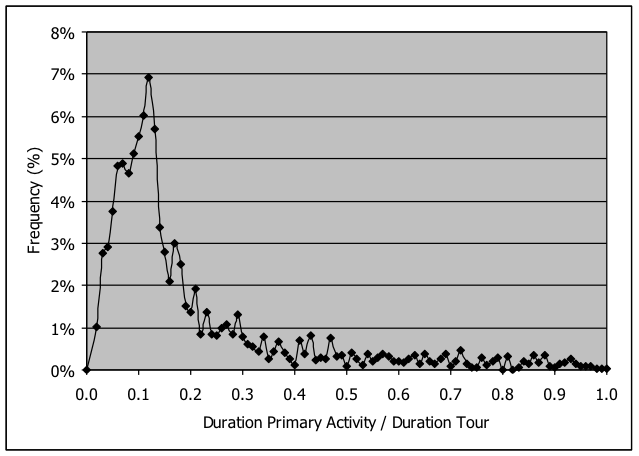
\includegraphics[width = 4in]{pt/excel-figures/figure7-7.png}} 
\subfloat[Cumulative work-based primary activity]{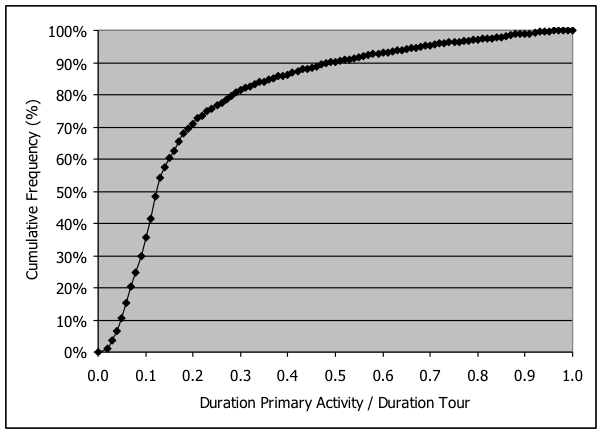
\includegraphics[width = 4in]{pt/excel-figures/figure7-8.png}} \\
\subfloat[First-at-work activity]{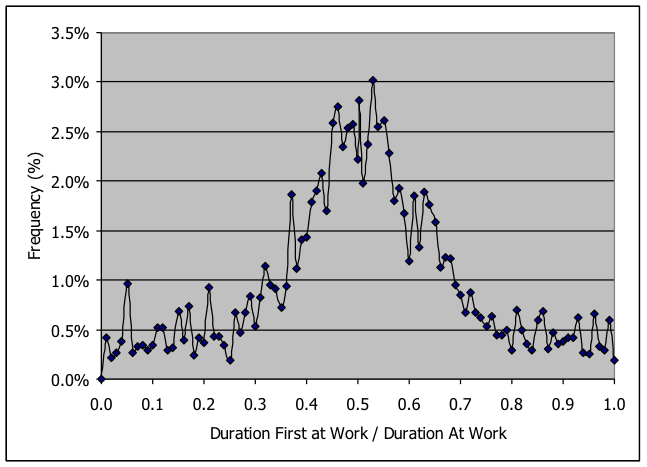
\includegraphics[width = 4in]{pt/excel-figures/figure7-9.png}}
\subfloat[Cumulative first-at-work activity]{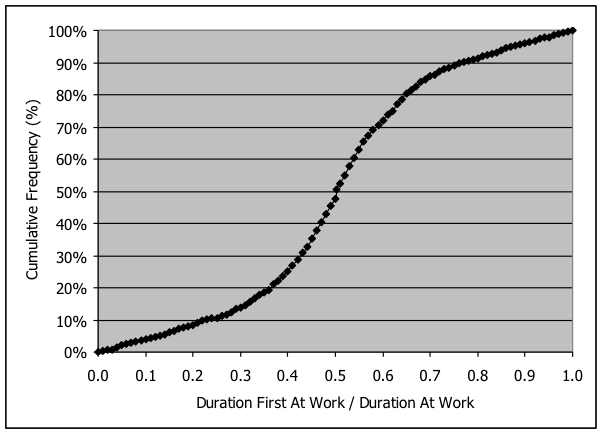
\includegraphics[width = 4in]{pt/excel-figures/figure7-10.png}} 
\caption{Observed frequency distributions for work-based activities}
\label{fig:pt-work-based-activity-duration-distributions}
\end{sidewaysfigure}

\subsection{LDT tour pattern model frequencies}
The LDT tour pattern model discussed in \S\ref{sec:ldt-tour-pattern} predicts the type of long-distance travel that occurs on the simulation day, if any. The model applies a set of factors, by purpose, derived from the Ohio survey data and assumed to be of the same pattern for Oregon. No further calibration is required. 

The Ohio survey-based tour pattern model observed frequency of each pattern type is shown in Table \ref{tab:ldt-tour-frequencies}. Because the model predicts typical weekday (Monday-Thursday) the weekends are excluded and thus work related travel is more likely to occur than household or other travel. Even with Fridays excluded, there are still more travelers departing during the week than returning.

\begin{table}  % 7 39
\centering
\caption{LDT tour pattern choice frequencies}\label{tab:ldt-tour-frequencies}
\begin{tabular}{lccc}
\hline
Pattern type & Household & Work-related & Other \\
\hline
Complete tour & 2.48 & 6.95 & 2.86 \\
\gray Begin tour & 2.37 & 4.72 & 2.11 \\
End tour & 2.03 & 3.36 & 1.71 \\
\gray Away & 7.90 & 11.26 & 5.43 \\
No tour & 85.21 & 73.71 & 87.88 \\
\hline
\multicolumn{3}{l}{\footnotesize Source: Ohio Statewide Model Program, LDT model estimation} \\
\end{tabular}
\end{table}

\subsection{LDT scheduling frequencies}
LDT tours are scheduled to a time-of-day with a one-hour resolution. Beginning tours are given a departure time, ending tours are given an arrival time and complete tours are given a departure time and duration to fully define their schedule. As with the LDT tour pattern model, the scheduling model draws from observed frequency distributions from the Ohio Long Distance Survey data. The Ohio-based departure time distribution for beginning tours and arrival time distribution for ending tours are shown in Figure \ref{fig:ldt-tours-hourly-distribution}. 

\begin{figure}  % 7.11
\centering
\includegraphics[width=6in, trim=0mm 5mm 0mm 0mm, clip]{pt/tours-hourly-distribution}  % l b r t
\caption{LDT departure times for beginning tours and arrival times for ending tours}
\label{fig:ldt-tours-hourly-distribution}
\end{figure}
 
For complete tours, the schedule is determined using a constants-only logit model, with constants on the departure time and duration. This strategy was applied to smooth the outcomes because the observed data had high unexplained variability when viewed in both dimensions. The choice set is restricted such that trips cannot depart before 5 AM or after 7 PM and all trips must return by 12 AM. The minimum duration is 2 hours and the maximum duration is 17 hours. Some changes were made to the model during calibration to better fit the observed departure time, arrival time and duration distributions. The final model coefficients are shown in Figure \ref{tab:ldt-complete-scheduling-coefficients}. They are estimated such that sequential two-hour periods have the same coefficient, to avoid high variability in the coefficient values. Mornings are popular departure times. The time periods after 3 PM have higher coefficients because the choice set is restricted such that those periods have fewer possible alternatives that can return by 12 AM.

\begin{table}  % 7-40
\centering
\caption{LDT complete tour scheduling model coefficients}\label{tab:ldt-complete-scheduling-coefficients}
\begin{tabular}{lr|lr|lr}
\hline
Variable & Coefficient & Variable & Coefficient & Variable & Coefficient \\
\hline
\multicolumn{2}{l|}{\textit{Duration constant}} & \multicolumn{2}{l|}{\textit{Departure time constant}} & \multicolumn{2}{l}{\textit{Arrival time constant}} \\
2 Hours & 0.959 & 5:00 AM & 0.000 & 9:00 PM & -1.174 \\
\gray 3 Hours & 1.609 & 6:00 AM &  & 10:00 PM & -1.457 \\
4 Hours & 2.544 & 7:00 AM & 1.033 & 11:00 PM & -2.440 \\
\gray 5 Hours & 2.898 & 8:00 AM & 1.944 \\
6 Hours & 3.278 & 9:00 AM & 2.216 &  &  \\
\gray 7 Hours & 3.518 & 10:00 AM & 1.459 \\
8 Hours &  & 11:00 AM & 1.423 &  & \\
\gray 9 Hours & 2.696 & 12:00 PM & \\
10 Hours &  & 1:00 PM & 1.392 &  & \\
\gray 11 Hours & 3.767 & 2:00 PM & \\
12 Hours &  & 3:00 PM & 2.457 &  & \\
\gray 13 Hours & 2.874 & 4:00 PM & \\
14 Hours &  & 5:00 PM & 3.027 &  &  \\
\gray 15 Hours & 2.964 & 6:00 PM & \\
16 Hours &  &  &  &  &  \\
\gray 17 Hours &  & \cellcolor{white} & \cellcolor{white} \\
\hline
\end{tabular}
\end{table}

\subsection{LDT internal-external choice model parameters}
The LDT internal-external choice model discussed in \S\ref{sec:ldt-internal-external} is a binary choice model predicting whether a tour will have a destination within the model area or beyond the bounds of the model area. All model coefficients are applied to the utility of leaving the model area. The models were calibrated to match the in-state versus out-of-state shares found in the Oregon section of the ATS for trips longer than 100 miles. The calibrated values are shown in Table \ref{tab:ldt-internal-external}.

\begin{table}
\centering
\caption{LDT internal-external model estimated coefficients}
\label{tab:ldt-internal-external}
\begin{tabular}{lrrr}
\hline
\multirow{2}{*}{Variable} & Household & Work-related & Other \\
 & coefficients & coefficients & coefficients \\
\hline
Constant & 1.6456 & 2.006 & 0.837 \\
\gray Income $>$\$60K & 0.441 &  &  \\
Occupation $=$ construction &  & -2.892 &  \\
\gray Occupation $=$ finance, insurance, real estate &  & -0.566 &  \\
Occupation $=$ public administration &  & -1.683 &  \\
\gray Occupation $=$ education &  & -1.426 &  \\
Occupation $=$ construction &  & -1.383 &  \\
\gray Person is a worker &  &  & -0.189 \\
Age $<$25 &  &  & -0.319 \\
\gray Age 55+ &  &  & 0.436 \\
Age 65+ &  & -1.155 & 0.436 \\
\gray Complete travel in one day & -2.084 & -2.707 & -1.458 \\
Time to nearest external station & -0.0084 &  & -0.0125 \\
\hline
\end{tabular}
\end{table}


%Table 7 41 LDT Internal-External Model Estimated Coefficients
%Variable       Household
%Coefficients   Work Related
%Coefficients   Other
%Coefficients
%Constant       1.6456  2.006   0.837
%Income <20k                        
%   $20-40k                     
%   $40-60k                     
%   $60k+   0.441           0.462
%Occupation Construction            -2.892      
%   Finance, insurance & real estate            -0.566      
%   Public administration           -1.683      
%   Education           -1.426      
%   Medical         -1.383      
%Person is a Worker                 -0.189
%Age    <25                 -0.319
%   55+                 0.436
%   65+         -1.155  0.436
%Complete Travel in One Day -2.084  -2.707  -1.458
%Time to Nearest External Station   -0.0084     -0.0125

\subsection{LDT destination choice model parameters}
The LDT destination choice models are applied separately for internal versus external destinations. The internal destination choice model parameters calibrated to Ohio trip length data, in the absence of comparable data from Oregon, are shown in Table \ref{tab:ldt-internal-destination-choice-coefficients}. Trips are distributed to external destinations through external stations (zones numbered in the 5000 range) using a simple destination choice model, which uses the highway travel time as the impedance and the traffic volume at the station as the size term. These model coefficients are shown in Table \ref{ldt-ext-dest-coefficients}. 

\begin{table}  % 7-42
\centering
\caption{LDT internal destination choice model estimated coefficients}
\label{tab:ldt-internal-destination-choice-coefficients}
\begin{tabular}{lrrr}
\hline
\multirow{2}{*}{Variable} & Household & Work-related & Other \\
 & coefficients & coefficients & coefficients \\
\hline
Mode choice logsum & 0.936 & 0.612 & 1.000 \\
\gray Time, if complete tour in one day & -0.016 & -0.012 & -0.011 \\
{\vspace{-9pt}} \\
\textit{Size terms} & & & \\
\gray ~~~Total households (a) & 2.793 &  & 1.958 \\
~~~Total employment & 1.000 & 1.000 & 1.000 \\
\gray ~~~Hotel -- if overnight trip (a) & 264.365 & 228.321 & 55.571 \\
~~~Higher education -- if age 18+ and student &  &  & 80.434 \\
\gray ~~~Government employment (a) &  & 7.057 &  \\
~~~Employment in worker's industry (a) &  & 3.671 &  \\
{\vspace{-9pt}} \\
\gray Flag for distance $<$60 miles & -0.167 & 0.286 & -1.514 \\
Flag for distance 60--70 miles & 0.738 & 1.026 & -0.940 \\
\gray Flag for distance 70--150 miles &  &  & -0.349 \\
\hline
\multicolumn{4}{l}{\footnotesize (a) Coefficient for application is exponential of reported coefficient.}
\end{tabular}
\end{table}

\begin{table}  % 7-43
\centering
\caption{LDT external destination choice model estimated coefficients}\label{ldt-ext-dest-coefficients}
\begin{tabular}{lccc}
\hline
\multirow{2}{*}{Variable} & Household & Work-related & Other \\
 & coefficients & coefficients & coefficients \\
\hline
Time & -0.0075 & -0.0075 & -0.0075 \\
\gray Size term (traffic volume) & 1 & 1 & 1 \\
\hline
\end{tabular}
\end{table}

\subsection{LDT mode choice model parameters}
The LDT mode choice model includes six alternatives, as shown in Table \ref{tab:ldt-internal-mode-choice-coefficients}.\footnote{Amtrak occupies the HSR choices in Oregon, a carryover from the Ohio model terminology.} As with destination choice, a simplified mode choice model is applied for trips with destinations outside the model area. In this case, fixed mode splits are applied, as derived from the Oregon segment of the 1995 American Travel Survey (ATS) data. 

\begin{table}  % 7-44
\centering
\caption{LDT internal mode choice model estimated coefficients}
\label{tab:ldt-internal-mode-choice-coefficients}
\begin{tabular}{lrrr}
\hline
 & Household & Work-related & Other \\
Variable & coefficients & coefficients & coefficients \\
\hline
In-vehicle time & -0.005 & -0.010 & -0.005 \\
\gray Walk-access time & -0.010 & -0.020 & -0.010 \\
Drive-access time & -0.010 & -0.020 & -0.010 \\
\gray Wait time -- up to 30 minutes & -0.010 & -0.020 & -0.010 \\
Wait time -- in excess of 30 minutes & -0.003 & -0.005 & -0.003 \\
\gray Cost (cents) -- income \$0-20K & -0.080 & -0.080 & -0.080 \\
Cost (cents) -- income \$20-60K & -0.030 & -0.030 & -0.030 \\
\gray Cost (cents) -- income \$60K+ & -0.012 & -0.012 & -0.012 \\
Transit-high speed rail nest & 0.650 & 0.650 & 0.650 \\
\gray Transit walk-drive nest & 0.500 & 0.500 & 0.500 \\
High speed rail walk-drive nest & 0.500 & 0.500 & 0.500 \\
\hline
\gray Air constant & -3.1870 & -1.0380 & -2.3020 \\
Transit walk access constant & -2.7973 & -2.7973 & -2.7973 \\
\gray Transit drive access constant & -2.7929 & -2.7929 & -2.7929 \\
High speed rail walk access constant & -4.4422 & -4.4422 & -4.4422 \\
\gray High school rail drive access constant & -4.4422 & -4.4422 & -4.4422 \\
\hline
\end{tabular}
\end{table}

\section{Inputs and Outputs}

The PT module inputs and outputs are listed in Tables \ref{tab:pt-generic-inputs} through \ref{tab:ldt-specific-inputs} and \ref{tab:ldt-sdt-outputs}, respectively. PT SDT inputs include the person and household attributes of the synthetic population generated by SPG, labor dollar flows from the AA module, travel attributes from VISUM, all in the current year. PT LDT inputs include external station traffic counts. Additionally, PT SDT and LDT requires some exogenous data including an alpha-to-beta zone mapping file, alpha zone acres and parking costs (daily and hourly), as well as files containing the parameters for each PT model. Currently only the weekday model of PT is used.

The primary PT output is a list of SDT and LDT trip tours for network assignment in VISUM. LDT also prints out an initial output, prior to additional processing into the format used by VISUM for assignment. PT also outputs mode choice and destination choice logsums by alpha zone for its own use and selected beta zone logsums for AA, additional household and person attributes tied to the synthetic population (autos and work location) and an employment summary (based on work location).

% This table is so long and difficult to squeeze to single page that we'll break it into three separate
% tables
\begin{table}  % Table 7-45
\centering
\caption{PT model inputs}\label{tab:pt-generic-inputs}
\begin{tabular}{L{3.2in} L{2.1in} l}
\hline
Data element & File(s) & Source \\
\hline
Lists (with attribute states) of modeled households resident in study area & SynPopH & SPG \\
\gray Lists (with attribute states) of modeled persons resident in study area & SynPopP & SPG \\
Peak and off-peak auto times and distances for interchanges between alpha zones, peak and off-peak walk-to/drive-to transit travel attributes & \*.zmx & VISUM \\
\gray Labor production (home end) and consumption (work end) 2009\$ by occupation in alpha zone & laborDollarProductionSum.csv, laborDollarConsumptionSum.csv & AA \\
Labor selling flows by industry (work trip ends) & selling\_commodity.csv & AA \\
\gray Solved beta zone industry-commodity production and consumption technical coefficients & ZonalMakeUse.csv & AA \\
Alpha zone acres and beta zones in alpha zones & alpha2beta.csv &	Exogenous \\
\gray Unit parking costs (work/nonwork) in alpha zones & alpha2beta.csv: fields ``HourPark'' and ``DayPark'' & Exogenous \\
Size term for LDT destination choice model & ExternalStationVolumes.csv & Exogenous \\
\hline
\end{tabular}
\end{table}

\begin{table}[!t]
\centering
\caption{SDT-specific model inputs}\label{tab:sdt-specific-inputs}
\begin{tabular}{L{2.85in} L{2.45in} l}
\hline
Data element & File(s) & Source \\
\hline
SDT HH survey observed activity patterns & weekdaypatterns.csv, patternAttributes.csv & Exogenous \\
\gray SDT auto ownership model parameters & autoownershipparameters.csv, globalTemplate.properties (latter from distance and time parameters) & Exogenous \\
SDT day pattern model parameters & weekdaypatternparameters.csv, patternparameters.csv & Exogenous \\
\gray SDT intermediate stop purpose model parameters & stoppurpose2tparameters.csv, stoppurpose3ptparameters.csv & Exogenous \\
SDT primary tour scheduling model parameters & TourScheduleParameters.csv & Exogenous \\
\gray Tour mode choice model parameters & tourmodeparameters.csv & Exogenous \\
SDT primary tour destination parameters & tourdestinationparameters.csv & Exogenous \\
\gray SDT intermediate stop model parameters & IntermediateStopChoiceParameters.csv, stopdestinationparameters.csv, firststopdestinationparameters.csv, secondstopdestiatinoparameters.csv & Exogenous \\
SDT trip mode choice model parameters & tripmodeparameters.csv & Exogenous \\
\gray SDT intermediate stop duration model parameters & stopDurationParameters.csv & Exogenous \\
SDT work-based trip duration model parameters & PctWorkBasedDuration.csv & Exogenous \\
\gray SDT cost inputs (walk, bike and drive to transit speeds, auto operating cost, time of first wait segment, non-work parking cost factor) & globalTemplate.properties & Exogenous \\
\hline
\end{tabular}
\end{table}

\begin{table}
\centering
\caption{LDT-specific model inputs}\label{tab:ldt-specific-inputs}
\begin{tabular}{L{2.55in} L{2.8in} l}
\hline
Data element & File(s) & Source \\
\hline
LDT binary choice of travel model parameters & LDTourBinaryChoiceParameters.csv & Exogenous \\
\gray LDT tour pattern model parameters & LDPatternModelFrequencies.csv & Exogenous \\
LDT scheduling model parameters & LDTourScheduleFrequencies.csv, DTourScheduleParameters.csv & Exogenous \\
\gray LDT internal-external choice model parameters & LDInternalExternalParameters.csv, LDExternalDestinationChoiceParameters.csv & Exogenous \\
LDT destination choice model parameters & LDExternalDestinationFrequencies.csv, LDInternalDestinationChoiceParameters.csv & Exogenous \\
\gray LDT mode choice model parameters & LDInternalModeChoiceParameters.csv, LDExternalModeChoiceParameters.csv, LDExternalModeShares.csv & Exogenous \\
LDT other inputs (rental car/taxi/airport parking costs, multi-day trip duration and auto occupancy by purpose) & globalTemplate.properties & Exogenous \\
\hline
\end{tabular}
\end{table}	
  % Table 7 45
\begin{table}  % 7 46
\centering
\caption{SDT and LDT outputs}\label{tab:ldt-sdt-outputs}
\begin{tabular}{L{3.3in} L{1.7in} l}
\hline
Data element & File(s) & Users \\
\hline
Selected mode travel utilities by market segment for interchanges between alpha zones (mode choice logsums) & \#\#mcls.zmx & PT (current year) \\
\gray Selected mode travel utilities by market segment for interchanges between beta zones (mode choice logsums) & \#\#betamcls.zmx & AA \\
Selected destination travel utilities for interchanges between alpha zones (destination choice logsums) & dcLogsums.zmx & PT (current year) \\
\gray Aggregate employment by industry and alpha zone & employment.csv & PT (next year) \\
Additional synthetic population person attributes identified within PT (linked to SynPopP by hhID and personID) & personData.csv & Diagnostics \\
\gray Additional synthetic population household attributes identified within PT (linked to SynPopH by hhID) & householdData.csv & Diagnostics \\
Alpha zone level summary of persons, household, workers & SynPop\_Taz\_Summary.csv & Diagnostics \\
\gray SDT daily pattern details & Patterns\_SDT.csv & Diagnostics \\
SDT person tour and trip details & Trips\_SDTPerson.csv & VISUM \\
\gray LDT person tour details & Tours\_LDT.csv & Diagnostics \\
LDT daily vehicle trips & Trips\_LDTVehicle.csv & Diagnostics \\
\gray LDT daily person trips & Trips\_LDTPerson.csv & VISUM \\
\hline
\end{tabular}
\end{table}
  % Table 7 46

The PT person trip table output used by the VISUM module has the following attributes:
\begin{itemize}
\item Origin alpha zone or external station
\item Destination alpha zone or external station
\item Distance
\item Origin Activity End Time (trip start time)
\item Primary Mode
\item Trip Mode
\end{itemize}

\subsection{Base year time and distance interchange matrices}
PT uses the time and distance interchange matrices (skims) created by VISUM, shown in Table \ref{tab:skims}. During calibration, an exogenous base year set of skims was developed. The base year SWIM2 transit skims were assembled primarily from mid-1990s MPO network data in EMME/2. Peak period skims were created using congested travel times from MPO model runs in the MPO portions of the network and free-flow travel times minus 5 mph in non-MPO areas. Off-peak skims used free-flow speeds. Once the statewide network was built, the skims were generated by EMME/2 using the MPO path-building parameters.
% The base year MPO network data and processing is described further in \ref{37}.

\begin{table}
\centering
\caption{Interchange matrices used by the PT models}\label{tab:skims}
\begin{tabular}{ll}
\hline
\multicolumn{2}{l}{\textit{Separate matrices for the peak and off-peak periods:}} \\
Walk-Transit In-vehicle Time & Drive-Transit In-vehicle Time \\
Walk-Transit First Wait & Drive-Transit First Wait \\
Walk-Transit Total Wait & Drive-Transit Total Wait \\
Walk-Transit Auxiliary Transit (WALK) Time & Drive-Transit Auxiliary Transit (WALK) Time \\
Walk-Transit Number Boardings & Drive-Transit Number Boardings \\
Walk-Transit Fare & Drive-Transit Drive Time \\
\hline
\end{tabular}
\end{table}

Once SWIM2 models are calibrated, the base year skims generated by VISUM replace the original base year inputs synthesized from MPO data. In application, all future year skims are output from VISUM and used in PT in the following (currently three-year) period.

\subsection{Other parameters}
A series of exogenous inputs are provided exogenously in the [globalTemplate.properties] file, under the AO and PT sections. These include the following, including their source data:
\begin{itemize}
\item Auto operating cost (this value is shared by SDT and LDT)
\item SDT speeds, wait time, parking factor: the following speeds and wait times were assumed:
\begin{itemize}
\item Walk speed (mph): 3 mph
\item Bike speed (mph): 12 mph
\item Drive to transit speed (mph): 25 mph
\item Time of first wait segment (minutes): 10 minutes
\item Non-work parking cost factor: 2.5
\end{itemize}
\item LDT-specific travel cost information: in addition to the transit costs associated with network skimming in VISUM, the following long distance travel costs are assumed in LDT. All are expressed in current 2009 dollars.
\begin{itemize}
\item Daily rental car costs: \$71.60/day
\item Taxi rate: \$2.15/minute
\item Daily airport parking costs: \$16.37/day
\end{itemize}
\item LDT average duration of a multi-day trip by purpose: 2.4, 4.6, and 2.6 hours for household, work-related, and other purpose, respectively.
\item LDT average auto occupancy by purpose, based upon the Ohio Long Distance Survey: 2.81, 1.22, and 1.91 hours for household, work-related, and other purpose, respectively.
\end{itemize}

\section{Calibration Targets}
During initial calibration, the PT module was formally compared to 14 sets of observed targets, to include household travel surveys, listed in Table \ref{tab:pt-calibration-targets}. Supplemental calibration targets are also listed. Transit boarding data from the major transit agencies in the state (typically annual or monthly boardings system-wide and/or by route) were compared with daily transit trips output by PT and VISUM. Census Journey to Work data commute trips (at a sub-county geographic scale) were used by PT (and AA) to calibrate the PT generated work trips (and AA labor flows).

\begin{sidewaystable}  % 7 47
\centering
\caption{PT calibration targets}\label{tab:pt-calibration-targets}
\begin{tabular}{lll}
\hline
Model & Source & SWIM2 targets \\
\hline
SDT & 1994/96 Oregon Travel & Average tours by purpose and MPO per household day \\
    & Behavior Surveys & Frequency of patterns by number of tours per pattern and MPO \\
    & & Average number of trips per household by MPO \\
    & & Frequency of tour departure time and duration and hour by MPO \\
    & & Average highway distance by tour purpose and MPO \\
\hline
SDT & 1990 and 2000 Census Journey & Commute trip data \\
    & to Work data \\
\hline
SDT & Local transit boarding data$^a$ & 1990 monthly passenger boardings \\
    & & July 1987--December 1999 (--August 1998 by route) monthly passengers \\
    & & 1987-96 average weekday boardings by route \\
    & & 1991-99 monthly ridership totals \\
    & & 1993 service performance and ridership by route \\
\hline
LDT & 1995 American Travel Survey & Number of trips $>$100 miles made by Oregon residents \\
    & Oregon element & Share of long-distance trips remaining within Oregon \\
    & & Share of auto versus non-auto long-distance trips \\
\hline
\multicolumn{3}{l}{\footnotesize a. Data provided by Tri-Met, Lane TD, Salem-Kaiser Transit, and Rogue Valley Transit.}
\end{tabular}
\end{sidewaystable}

\subsection{Initial calibration}
The PT module was updated in fall 2006 to add the LDT component and update various SDT components enhanced in Ohio application. After code changes were made, both the SDT and LDT components completed S2 calibration, in isolation of other modules. 

\subsection{SDT calibration}
The initial calibration of the SDT component of PT was based on a five percent population sample model estimates. The results were factored by the sampling rate so they are representative of the entire population. Once the model was well-calibrated, a 100 percent population run was completed and the results were compared to the target data.

\subsubsection{Day-pattern choice model}
The PT day-pattern choice model was calibrated to match the targets shown below. The PT parameters control for the choice of pattern with respect to specific pattern attributes (i.e., numbers and types of activities on pattern) for each person type. 
The calibration results for the distribution of patterns by the number of tours in the pattern, for all of Oregon plus Clark County in Washington and MPO regions, are shown in Table \ref{tab:patterns-by-number-of-tours}. The model matches the targets in terms of total patterns produced, statewide and by MPO region. It tends to over-predict the longest patterns, which are also the least frequent ones.

\begin{small}
\begin{longtable}{lcrrrrrr}
\caption{\normalsize{Patterns by number of tours per pattern}}\vspace{-9pt} \\ 
\hline
 & Number & \multicolumn{2}{c}{Target} & \multicolumn{2}{c}{Estimate} & \multicolumn{2}{c}{Error} \\
\cline{3-4}\cline{5-6}\cline{7-8}
Area & of tours & Frequency & Percent & Frequency & Percent & Frequency & Percent \\
\hline
\endfirsthead
\hline
 & Number & \multicolumn{2}{c}{Target} & \multicolumn{2}{c}{Estimate} & \multicolumn{2}{c}{Error} \\
\cline{3-4}\cline{5-6}\cline{7-8}
Area & of tours & Frequency & Percent & Frequency & Percent & Frequency & Percent \\
\hline
\endhead
\hline \multicolumn{8}{r}{\emph{Continued on next page}}
\endfoot
\hline
\endlastfoot\label{tab:patterns-by-number-of-tours}
Oregon and & 0 & 641,444 & 16.8 & 694,900 & 18 & 53,456 & 8.3 \\
\gray \cellcolor{white}Clark County & 1 & 1,852,901 & 48.5 & 1,850,046 & 47.9 & -2,855 & -0.2 \\
 & 2 & 987,231 & 25.9 & 978,941 & 25.4 & -8,290 & -0.8 \\
\gray \cellcolor{white} & 3 & 269,184 & 7 & 268,052 & 6.9 & -1,132 & -0.4 \\
 & 4 & 53,012 & 1.4 & 54,351 & 1.4 & 1,339 & 2.5 \\
\gray \cellcolor{white} & 5 & 12,364 & 0.3 & 11,190 & 0.3 & -1,174 & -9.5 \\
 & 6 & 1,980 & 0.1 & 2,727 & 0.1 & 747 & 37.7 \\
\gray \cellcolor{white} & 7 & 553 & 0 & 863 & 0 & 310 & 56.1 \\
 & 8 & 68 & 0 & 279 & 0 & 211 & 310.3 \\
\gray \cellcolor{white} & Total & 3,818,737 & 100 & 3,861,349 & 100 & 42,612 & 1.1 \\
\hline
Portland & 0 & 242,312 & 14 & 314,081 & 17.7 & 71,769 & 29.6 \\
\gray \cellcolor{white} & 1 & 865,862 & 49.9 & 837,464 & 47.1 & -28,398 & -3.3 \\
 & 2 & 483,257 & 27.9 & 458,169 & 25.8 & -25,088 & -5.2 \\
\gray \cellcolor{white} & 3 & 116,676 & 6.7 & 132,824 & 7.5 & 16,148 & 13.8 \\
 & 4 & 20,567 & 1.2 & 27,449 & 1.5 & 6,882 & 33.5 \\
\gray \cellcolor{white} & 5 & 5,104 & 0.3 & 5,945 & 0.3 & 841 & 16.5 \\
 & 6 & 565 & 0 & 1,434 & 0.1 & 869 & 153.8 \\
\gray \cellcolor{white} & 7 & 331 & 0 & 467 & 0 & 136 & 41.1 \\
 & 8 & 44 & 0 & 150 & 0 & 106 & 240.9 \\
\gray \cellcolor{white} & Total & 1,734,718 & 100 & 1,777,983 & 100 & 43,265 & 2.5 \\
\hline
Salem & 0 & 29,407 & 14.3 & 37,079 & 17.6 & 7,672 & 26.1 \\
\gray \cellcolor{white} & 1 & 97,526 & 47.4 & 95,432 & 45.4 & -2,094 & -2.1 \\
 & 2 & 57,230 & 27.8 & 56,476 & 26.8 & -754 & -1.3 \\
\gray \cellcolor{white} & 3 & 17,600 & 8.6 & 16,771 & 8 & -829 & -4.7 \\
 & 4 & 3,051 & 1.5 & 3,614 & 1.7 & 563 & 18.5 \\
\gray \cellcolor{white} & 5 & 735 & 0.4 & 734 & 0.3 & -1 & -0.1 \\
 & 6 & 84 & 0 & 216 & 0.1 & 132 & 157.1 \\
\gray \cellcolor{white} & 7 & 96 & 0 & 61 & 0 & -35 & -36.5 \\
 & 8 &  &  & 24 & 0 & 24 &  \\
\gray \cellcolor{white} & Total & 205,729 & 100 & 210,407 & 99.9 & 4,678 & 2.3 \\
\hline
Eugene & 0 & 37,325 & 14.2 & 45,690 & 17.8 & 8,365 & 22.4 \\
\gray \cellcolor{white} & 1 & 120,499 & 46 & 116,751 & 45.6 & -3,748 & -3.1 \\
 & 2 & 74,094 & 28.3 & 67,956 & 26.5 & -6,138 & -8.3 \\
\gray \cellcolor{white} & 3 & 24,166 & 9.2 & 20,173 & 7.9 & -3,993 & -16.5 \\
 & 4 & 4,793 & 1.8 & 4,406 & 1.7 & -387 & -8.1 \\
\gray \cellcolor{white} & 5 & 867 & 0.3 & 844 & 0.3 & -23 & -2.7 \\
 & 6 & 266 & 0.1 & 237 & 0.1 & -29 & -10.9 \\
\gray \cellcolor{white} & 7 & 63 & 0 & 80 & 0 & 17 & 27 \\
 & 8 &  &  & 23 & 0 & 23 &  \\
\gray \cellcolor{white} & Total & 262,073 & 99.9 & 256,160 & 99.9 & -5,913 & -2.3 \\
\hline
Medford & 0 & 30,706 & 20.2 & 27,509 & 17.7 & -3,197 & -10.4 \\
\gray \cellcolor{white} & 1 & 70,553 & 46.4 & 71,496 & 46.1 & 943 & 1.3 \\
 & 2 & 36,393 & 23.9 & 41,343 & 26.7 & 4,950 & 13.6 \\
\gray \cellcolor{white} & 3 & 11,642 & 7.7 & 11,665 & 7.5 & 23 & 0.2 \\
 & 4 & 2,176 & 1.4 & 2,415 & 1.6 & 239 & 11 \\
\gray \cellcolor{white} & 5 & 463 & 0.3 & 492 & 0.3 & 29 & 6.3 \\
 & 6 & 73 & 0 & 114 & 0.1 & 41 & 56.2 \\
\gray \cellcolor{white} & 7 &  &  & 48 & 0 & 48 &  \\
 & 8 &  &  & 11 & 0 & 11 &  \\
\gray \cellcolor{white} & Total & 152,006 & 99.9 & 155,093 & 100 & 3,087 & 2 \\
\hline
Non-MPO & 0 & 301,786 & 20.6 & 270,541 & 18.5 & -31,245 & -10.4 \\
\gray \cellcolor{white} & 1 & 698,462 & 47.7 & 728,903 & 49.9 & 30,441 & 4.4 \\
 & 2 & 336,257 & 23 & 354,997 & 24.3 & 18,740 & 5.6 \\
\gray \cellcolor{white} & 3 & 99,100 & 6.8 & 86,619 & 5.9 & -12,481 & -12.6 \\
 & 4 & 22,424 & 1.5 & 16,467 & 1.1 & -5,957 & -26.6 \\
\gray \cellcolor{white} & 5 & 5,196 & 0.4 & 3,175 & 0.2 & -2,021 & -38.9 \\
 & 6 & 992 & 0.1 & 726 & 0 & -266 & -26.8 \\
\gray \cellcolor{white} & 7 & 63 & 0 & 207 & 0 & 144 & 228.6 \\
 & 8 & 24 & 0 & 71 & 0 & 47 & 195.8 \\
\gray \cellcolor{white} & Total & 1,464,304 & 100.1 & 1,461,706 & 99.9 & -2,598 & -0.2 \\
\end{longtable}
\end{small}  % Tables 7-48 to 7-53, now combined into single table

\subsubsection{Frequency of tours by tour purpose}
The calibration results for the distribution of tours by tour purpose, for all of Oregon plus Clark County in Washington and by MPO region, are shown in Table \ref{tab:pt-tours-by-tour-purpose}. Statewide the model is matching the number of work and school tours, over-estimating shop and recreation tours, and underestimating other tours. At the MPO level the most noticeable difference is the over-estimation of work tours in Salem and Medford.

\begin{table}
\centering
\caption{Tours by tour purpose by MPO region}\label{tab:pt-tours-by-tour-purpose}
%\renewcommand{\arraystretch}{0.95}
\small
\begin{tabular}{llrrrrrr}
\hline
     &              & \multicolumn{2}{c}{Target} & \multicolumn{2}{c}{Estimate} & \multicolumn{2}{c}{Error} \\
\cline{3-4}\cline{5-6}\cline{7-8}
Area & Tour purpose & Frequency & Percent & Frequency & Percent & Frequency & Percent \\
\hline
Oregon and & Work--no subtour & 968,715 & 26.4 & 1,046,260 & 27.2 & 77,545 & 8 \\
\gray \cellcolor{white}Clark County & Work--with subtour & 235,073 & 6.4 & 244,813 & 6.4 & 9,740 & 4.1 \\
 & School & 643,757 & 17.6 & 609,172 & 15.8 & -34,585 & -5.4 \\
\gray \cellcolor{white} & Shop & 64,398 & 1.8 & 119,567 & 3.1 & 55,169 & 85.7 \\
 & Recreation & 864,356 & 23.6 & 904,497 & 23.5 & 40,141 & 4.6 \\
\gray \cellcolor{white} & Other & 889,425 & 24.3 & 919,294 & 23.9 & 29,869 & 3.4 \\
 & Total & 3,665,724 & 100.1 & 3,843,603 & 99.9 & 177,879 & 4.9 \\
\hline
\gray \cellcolor{white}Portland & Work--no subtour & 477,814 & 27.8 & 497,364 & 27.7 & 19,550 & 4.1 \\
 & Work--with subtour & 91,641 & 5.3 & 114,353 & 6.4 & 22,712 & 24.8 \\
\gray \cellcolor{white} & School & 298,944 & 17.4 & 274,332 & 15.3 & -24,612 & -8.2 \\
 & Shop & 39,296 & 2.3 & 55,869 & 3.1 & 16,573 & 42.2 \\
\gray \cellcolor{white} & Recreation & 405,532 & 23.6 & 427,092 & 23.7 & 21,560 & 5.3 \\
 & Other & 404,647 & 23.6 & 429,622 & 23.9 & 24,975 & 6.2 \\
\gray \cellcolor{white} & Total & 1,717,874 & 100 & 1,798,632 & 100.1 & 80,758 & 4.7 \\
\hline
Salem & Work--no subtour & 42,914 & 21.1 & 56,827 & 26.4 & 13,913 & 32.4 \\
\gray \cellcolor{white} & Work--with subtour & 15,245 & 7.5 & 13,005 & 6 & -2,240 & -14.7 \\
 & School & 33,563 & 16.5 & 33,451 & 15.5 & -112 & -0.3 \\
\gray \cellcolor{white} & Shop & 467 & 0.2 & 6,448 & 3 & 5,981 & 1280.7 \\
 & Recreation & 52,794 & 25.9 & 53,071 & 24.6 & 277 & 0.5 \\
\gray \cellcolor{white} & Other & 58,710 & 28.8 & 52,548 & 24.4 & -6,162 & -10.5 \\
 & Total & 203,693 & 100 & 215,350 & 99.9 & 11,657 & 5.7 \\
\hline
\gray \cellcolor{white}Eugene & Work--no subtour & 67,389 & 24.1 & 68,092 & 26.2 & 703 & 1 \\
 & Work--with subtour & 20,455 & 7.3 & 15,556 & 6 & -4,899 & -24 \\
\gray \cellcolor{white} & School & 44,793 & 16 & 37,877 & 14.6 & -6,916 & -15.4 \\
 & Shop & 2,258 & 0.8 & 8,661 & 3.3 & 6,403 & 283.6 \\
\gray \cellcolor{white} & Recreation & 71,614 & 25.6 & 65,407 & 25.1 & -6,207 & -8.7 \\
 & Other & 73,230 & 26.2 & 64,717 & 24.9 & -8,513 & -11.6 \\
\gray \cellcolor{white} & Total & 279,739 & 100 & 260,310 & 100.1 & -19,429 & -6.9 \\
\hline
Medford & Work--no subtour & 27,922 & 19.9 & 40,682 & 25.9 & 12,760 & 45.7 \\
\gray \cellcolor{white} & Work--with subtour & 8,619 & 6.1 & 9,326 & 5.9 & 707 & 8.2 \\
 & School & 21,294 & 15.2 & 24,407 & 15.6 & 3,113 & 14.6 \\
\gray \cellcolor{white} & Shop & 1,652 & 1.2 & 5,062 & 3.2 & 3,410 & 206.4 \\
 & Recreation & 40,670 & 28.9 & 39,022 & 24.9 & -1,648 & -4.1 \\
\gray \cellcolor{white} & Other & 40,370 & 28.7 & 38,419 & 24.5 & -1,951 & -4.8 \\
 & Total & 140,527 & 100 & 156,918 & 100 & 16,391 & 11.7 \\
\hline
\gray \cellcolor{white}Non-MPO & Work--no subtour & 352,676 & 26.6 & 383,295 & 27.1 & 30,619 & 8.7 \\
 & Work--with subtour & 99,114 & 7.5 & 92,573 & 6.6 & -6,541 & -6.6 \\
\gray \cellcolor{white} & School & 245,164 & 18.5 & 239,105 & 16.9 & -6,059 & -2.5 \\
 & Shop & 20,724 & 1.6 & 43,527 & 3.1 & 22,803 & 110 \\
\gray \cellcolor{white} & Recreation & 293,747 & 22.2 & 319,905 & 22.6 & 26,158 & 8.9 \\
 & Other & 312,468 & 23.6 & 333,988 & 23.6 & 21,520 & 6.9 \\
\gray \cellcolor{white} & Total & 1,323,893 & 100 & 1,412,393 & 99.9 & 88,500 & 6.7 \\\hline
\end{tabular}
\end{table}   % Tables 7-54 through 7-59, now combined into single table

\subsubsection{Frequency of trips by tour purpose}
The calibration results for the distribution of trips by tour purpose, for all of Oregon plus Clark County in Washington and MPO region, are shown in Table \ref{tab:pt-trips-by-tour-purpose}. Statewide the model overestimates the number of trips on work, shop and recreation tours and underestimates the number of trips on school, other and college tours. Together with the results for tours by tour purpose, this indicates that the model tends to over-select patterns with multiple stops on work tours and under-select patterns with multiple stops on school tours. The results for shop, recreation and other tours may be directly a result of the tour purpose distribution rather than related to the stops.

\begin{table}
\centering
\caption{Trips by tour purpose by MPO region}\label{tab:pt-trips-by-tour-purpose}
\renewcommand{\arraystretch}{0.95}
\small
\begin{tabular}{llrrrrrr}
\hline
 & & \multicolumn{2}{c}{Target} & \multicolumn{2}{c}{Estimate} & \multicolumn{2}{c}{Error} \\
\cline{3-4}\cline{5-6}\cline{7-8}
Area & Tour purpose & Frequency & Percent & Frequency & Percent & Frequency & Percent \\
\hline
Oregon and & Work--no subtour & 2,348,106 & 18.8 & 2,483,861 & 22.4 & 135,755 & 5.8 \\
\gray \cellcolor{white}Clark County & Work--with subtour & 597,642 & 4.8 & 625,615 & 5.6 & 27,973 & 4.7 \\
 & School & 1,525,040 & 12.2 & 1,378,017 & 12.4 & -147,023 & -9.6 \\
\gray \cellcolor{white} & College & 1,673,953 & 13.4 & 308,150 & 2.8 & -1,365,803 & -81.6 \\
 & Shop & 2,214,399 & 17.7 & 2,284,009 & 20.6 & 69,610 & 3.1 \\
\gray \cellcolor{white} & Recreation & 1,984,808 & 15.9 & 2,060,727 & 18.6 & 75,919 & 3.8 \\
 & Other & 2,152,554 & 17.2 & 1,960,045 & 17.7 & -192,509 & -8.9 \\
\gray \cellcolor{white} & Total & 12,496,502 & 100 & 11,100,424 & 100.1 & -1,396,078 & -11.2 \\
\hline
Portland & Work--no subtour & 1,169,683 & 20 & 1,173,609 & 22.7 & 3,926 & 0.3 \\
\gray \cellcolor{white} & Work--with subtour & 231,965 & 4 & 290,627 & 5.6 & 58,662 & 25.3 \\
 & School & 693,251 & 11.8 & 615,207 & 11.9 & -78,044 & -11.3 \\
\gray \cellcolor{white} & College & 784,907 & 13.4 & 141,427 & 2.7 & -643,480 & -82 \\
 & Shop & 1,031,815 & 17.6 & 1,062,827 & 20.6 & 31,012 & 3 \\
\gray \cellcolor{white} & Recreation & 903,687 & 15.4 & 955,544 & 18.5 & 51,857 & 5.7 \\
 & Other & 1,035,536 & 17.7 & 928,052 & 18 & -107,484 & -10.4 \\
\gray \cellcolor{white} & Total & 5,850,844 & 99.9 & 5,167,293 & 100 & -683,551 & -11.7 \\
\hline
Salem & Work--no subtour & 105,909 & 15.1 & 133,777 & 21.4 & 27,868 & 26.3 \\
\gray \cellcolor{white} & Work--with subtour & 39,872 & 5.7 & 32,834 & 5.3 & -7,038 & -17.7 \\
 & School & 77,325 & 11 & 75,050 & 12 & -2,275 & -2.9 \\
\gray \cellcolor{white} & College & 78,337 & 11.2 & 16,256 & 2.6 & -62,081 & -79.2 \\
 & Shop & 131,422 & 18.8 & 131,718 & 21.1 & 296 & 0.2 \\
\gray \cellcolor{white} & Recreation & 134,626 & 19.2 & 116,516 & 18.7 & -18,110 & -13.5 \\
 & Other & 132,973 & 19 & 117,620 & 18.9 & -15,353 & -11.5 \\
\gray \cellcolor{white} & Total & 700,464 & 100 & 623,771 & 100 & -76,693 & -10.9 \\
\hline
Eugene & Work--no subtour & 167,499 & 18.2 & 160,779 & 21.2 & -6,720 & -4 \\
\gray \cellcolor{white} & Work--with subtour & 52,517 & 5.7 & 39,370 & 5.2 & -13,147 & -25 \\
 & School & 106,493 & 11.6 & 84,817 & 11.2 & -21,676 & -20.4 \\
\gray \cellcolor{white} & College & 112,133 & 12.2 & 21,941 & 2.9 & -90,192 & -80.4 \\
 & Shop & 182,001 & 19.8 & 162,581 & 21.5 & -19,420 & -10.7 \\
\gray \cellcolor{white} & Recreation & 162,504 & 17.7 & 143,713 & 19 & -18,791 & -11.6 \\
 & Other & 136,363 & 14.8 & 143,472 & 19 & 7,109 & 5.2 \\
\gray \cellcolor{white} & Total & 919,510 & 100 & 756,673 & 100 & -162,837 & -17.7 \\
\hline
Medford & Work--no subtour & 68,051 & 14.4 & 96,206 & 21.1 & 28,155 & 41.4 \\
\gray \cellcolor{white} & Work--with subtour & 22,025 & 4.7 & 23,834 & 5.2 & 1,809 & 8.2 \\
 & School & 49,446 & 10.5 & 54,865 & 12 & 5,419 & 11 \\
\gray \cellcolor{white} & College & 53,171 & 11.2 & 12,983 & 2.8 & -40,188 & -75.6 \\
 & Shop & 104,644 & 22.1 & 97,901 & 21.4 & -6,743 & -6.4 \\
\gray \cellcolor{white} & Recreation & 90,122 & 19.1 & 85,769 & 18.8 & -4,353 & -4.8 \\
 & Other & 85,568 & 18.1 & 85,079 & 18.6 & -489 & -0.6 \\
\gray \cellcolor{white} & Total & 473,027 & 100.1 & 456,637 & 99.9 & -16,390 & -3.5 \\
\hline
Non-MPO & Work--no subtour & 836,965 & 18.4 & 919,490 & 22.4 & 82,525 & 9.9 \\
\gray \cellcolor{white} & Work--with subtour & 251,263 & 5.5 & 238,950 & 5.8 & -12,313 & -4.9 \\
 & School & 598,525 & 13.1 & 548,078 & 13.4 & -50,447 & -8.4 \\
\gray \cellcolor{white} & College & 645,404 & 14.2 & 115,543 & 2.8 & -529,861 & -82.1 \\
 & Shop & 764,517 & 16.8 & 828,982 & 20.2 & 64,465 & 8.4 \\
\gray \cellcolor{white} & Recreation & 693,868 & 15.2 & 759,185 & 18.5 & 65,317 & 9.4 \\
 & Other & 762,114 & 16.7 & 685,822 & 16.7 & -76,292 & -10 \\
\gray \cellcolor{white} & Total & 4,552,656 & 99.9 & 4,096,050 & 99.8 & -456,606 & -10 \\
\hline
\end{tabular}
\end{table}  % Replaces Tables 7-60 through 7-65

\subsubsection{Workplace location model}
The comparison of work tour lengths for all income groups is shown in Figure \ref{fig:pt-home-work-distance-calibration}. The model matches well the target tour length (home to work, one way) overall, but does not match well differences by income group. The income groups can be adjusted within the AA module and that is a recommended next step for the model.

\begin{figure}  % Figure 7.12
\centering
\includegraphics[width=4.5in]{pt/excel-figures/figure7-12.png}
\caption{Calibration results for home-to-work distance}
\label{fig:pt-home-work-distance-calibration}
\end{figure}

\subsubsection{Tour primary destination choice model}
This model has been calibrated to match average tour length by tour purpose, statewide and the percent of intrazonal tours, also statewide. The calibration consists of adjusting the coefficients for tour distance and for the intrazonal indicator variable. The comparison to the target data is shown in Table \ref{tab:average-tour-length-percent-intrazonal}.

% This table was marked as 7-68 in the text, but actually refers to Figure 7-12 (a table pasted in as a figure)
\begin{table}
\centering
\caption{Average tour length and percent intrazonal tours}\label{tab:average-tour-length-percent-intrazonal}
\begin{tabular}{lrrrrcrrr}
\hline
 & \multicolumn{4}{c}{Average tour length (miles)} &  & \multicolumn{3}{c}{Percent interzonal trips} \\
\cline{2-5}\cline{7-9}
Tour purpose & Target & Estimate & Error & \% error & & Target & Estimate & Error (\%) \\
\hline
School & 9.5 & 9.4 & -0.1 & -1.1 & & 16.3 & 15.2 & -1.0 \\
\gray College & 15.6 & 16.8 & 1.2 & 7.7 & & 6.1 & 5.5 & -0.6 \\
Shop & 14.4 & 14.6 & 0.2 & 1.4 & & 6.5 & 6.1 & -0.4 \\
\gray Recreation & 12.8 & 13.7 & 0.9 & 7.0 & & 11.4 & 10.9 & -0.5 \\
Other & 11.0 & 11.0 & 0.0 & 0.0 & & 9.1 & 8.3 & -0.8 \\
\gray Subtours & 8.1 & 8.3 & 0.2 & 2.5 & & 4.7 & 8.1 & 3.4 \\
\hline
\end{tabular}
\end{table}

\subsubsection{Tour schedule choice model}
This model has been calibrated to match the distribution of departure time and duration by tour purpose, statewide. The calibration consisted of adjusting the alternative-specific constants. The comparison to the target data is shown in Figures \ref{fig:pt-tour-departure-times-redux} (departure time) and \ref{fig:pt-tour-durations-redux} (duration). The model was also compared to several other targets:

\begin{sidewaysfigure}  % Figures 7.14 through 7.28
\centering
\includegraphics[scale=0.9]{pt/pt-tour-departure-hours-redux}
\caption{Observed versus estimated tour departure hours by tour type}
\label{fig:pt-tour-departure-times-redux}
\end{sidewaysfigure}

\begin{sidewaysfigure}  % Figures 7.19 through 7.23
\centering
\includegraphics[scale=0.9]{pt/pt-tour-durations-redux}
\caption{Observed versus estimated tour durations by tour type}
\label{fig:pt-tour-durations-redux}
\end{sidewaysfigure}

\begin{itemize}
\item The auto ownership model was calibrated to match targets developed from the Oregon survey data. The number of households within the zero, one, two or three or more vehicles was matched within 2 percent of the target data statewide.
\item The PT SDT intermediate stop location model was calibrated to match average deviation distance by mode, percent of stops in the home alpha zone by mode and percent of stops in the primary destination alpha zone by mode. The calibration consists of adjusting the coefficients on out-of-direction time and intrazonal indicator variables. An initial calibration showed that the model was not able to reproduce observed differences in trip length by inbound/outbound stop. The model has been modified so that the time and intrazonal variables are now segmented by stop position; further calibration of these segmented parameters is underway.
\item The PT SDT intermediate stop duration model was calibrated to match the distribution of stop duration by tour purpose and stop position (outbound/inbound). The calibration consisted of adjusting the alternative-specific constants and the outbound stop indicator variable.
\item The PT SDT tour primary mode choice model was calibrated to the frequency of tours by market segment (car sufficiency). The calibration consists of adjusting the alternative-specific constants until each segment is within 10 percent of the target. 
\item The PT SDT trip mode choice model was calibrated to frequency of trips by primary mode. The calibration consists of adjusting the alternative-specific constants until each segment is within 10 percent of the target.
\end{itemize}

\subsection{LDT calibration}

\subsubsection{Binary choice of travel}
The results of the binary choice of travel model by purpose compared to the 1995 American Travel Survey calibration targets are shown in Table \ref{tab:ats-long-tours}. Overall, the highest rate of travel is for other tours, at 33 percent and the lowest is for work related tours, at four percent. According to the target data, the frequency of long distance travel is greater in Oregon than in Ohio, perhaps because of income and geographic differences.

\begin{table}
\centering
\caption{Percent of persons making long distance tour in a two-week period}\label{tab:ats-long-tours}
\begin{tabular}{lrrr}
\hline
Tour purpose & Observed & Modeled & Difference \\
\hline
Household & 16.8 & 17.9 & 1.1 \\
\gray Work-related & 3.8 & 4.1 & 0.3 \\
Other & 33 & 35.2 & 2.2 \\
\gray Total & 47.7 & 47.4 & -0.3 \\
\hline
\multicolumn{4}{l}{\footnotesize Note: All values shown are percentages.} \\
\end{tabular}
\end{table}

\subsubsection{Tour pattern}
While the LDT tour pattern model itself requires no calibration, when combined with the binary choice of travel model, it results in the total trips generated. The total number of long distance trips occurring on the travel day and the subset of those that are greater than 100 miles, summarized from the ATS, are shown in Table \ref{tab:ats-distances}.

\begin{table}
\centering
\caption{Total trips on model day}\label{tab:ats-distances}
\begin{tabular}{lrrrr}
\hline
Range & Observed & Modeled & Difference & \% difference \\
\hline
$>$50 miles &  & 257,152 &  &  \\
\gray $>$100 miles & 157,272 & 157,684 & 412 & 0.3 \\
\hline
\end{tabular}
\end{table}

\subsubsection{Scheduling}
The scheduling model draws from observed frequency distributions for beginning tours and ending tours, which is assumed to be the same in Oregon as in Ohio. No calibration was required for the departure time of beginning tours or the arrival time of ending tours, shown in Figure \ref{figure7.13}. The modeled and observed departure times, as well as arrival times and durations for the complete tour scheduling model, are shown in Figures \ref{fig:pt-tour-departure-arrival-times} and \ref{fig:pt-complete-tours-duration}.

\begin{sidewaysfigure}  % Figures 7.24 and 7.25
\centering
\subfloat[Departure time for begin tours]{\includegraphics[width = 4in]{pt/excel-figures/figure7-24a.png}} 
\subfloat[Arrival time for end tours]{\includegraphics[width = 4in]{pt/excel-figures/figure7-24b.png}} \\
\subfloat[Departure time for complete tours]{\includegraphics[width = 4in]{pt/excel-figures/figure7-25a.png}}
\subfloat[Arrival time for complete tours]{\includegraphics[width = 4in]{pt/excel-figures/figure7-25b.png}} 
\caption{Tour departure and arrival times}
\label{fig:pt-tour-departure-arrival-times}
\end{sidewaysfigure}

\begin{figure}   % Figure 7.26
\centering
\includegraphics[width=4.25in]{pt/excel-figures/figure7-26.png}
\caption{Duration for complete tours}
\label{fig:pt-complete-tours-duration}
\end{figure}

\subsubsection{Internal-external choice}
The LDT internal-external choice models were calibrated to match the in-state versus out-of-state shares found in the ATS for trips longer than 100 miles. The model calibration results are shown in table \ref{tab:pt-internal-external-calibration}. Because the length of external trips is not known beyond the model area, all external trips are assumed to be longer than 100 miles for comparison to the ATS.

\begin{table}  % 7 68
\centering
\caption{Internal-external model calibration results}\label{tab:pt-internal-external-calibration}
\begin{tabular}{lrrrr}
\hline
 & \multicolumn{4}{c}{Trips $>$100 miles} \\
Trip type & Observed & Modeled & Difference & \% difference \\
\hline 
Internal & 64,836 & 67,282 & 2,446 & 3.8 \\
\gray External & 92,436 & 90,402 & -2,034 & -2.2 \\
Total & 157,272 & 157,684 & 412 & 0.3 \\
\hline
\end{tabular}
\end{table}

\subsubsection{Destination choice}
The LDT destination choice models are applied separately for internal versus external destinations. To calibrate the models, the distance flags were adjusted to properly match the number of trips in three distance bands: less than 60 miles, 60 to 70 miles and 70 to 150 miles. The inclusion of these distance band constants allows the model to match the observed trip length distributions without modifying the mode choice logsum coefficients. The observed trip lengths and trip length distributions are taken from the Ohio data, because no such information is available in the ATS. If data becomes available that is specific to Oregon, these models can be recalibrated. 

The modeled and observed average trip lengths are shown in Table \ref{tab:internal-destinations-average-distances}, while the modeled and observed trip length distributions by purpose are shown in Figure \ref{fig:pt-trip-length-distributions-destinations}. Due to relatively small sample sizes, the observed distributions are somewhat lumpy, but the models generally match those curves well.

\begin{table}   % 7 69
\centering
\caption{Average Trip lengths of tours with internal destinations}
\label{tab:internal-destinations-average-distances}
\begin{tabular}{llrrrr}
\hline
Tour type & Tour category & Observed & Modeled & Difference & \% difference \\
\hline
Household & Begin and end tours & 131.4 & 165 & 33.6 & 25.6 \\
\gray \cellcolor{white} & Complete tours & 89.4 & 97.4 & 8 & 8.9 \\
 & Total & 101.3 & 116.5 & 15.2 & 15 \\
\hline
\gray \cellcolor{white}Work-related & Begin and end tours & 130.6 & 155.5 & 24.9 & 19.1 \\
 & Complete tours & 90.8 & 98.9 & 8.1 & 8.9 \\
\gray \cellcolor{white} & Total & 97.5 & 108.4 & 10.9 & 11.2 \\
\hline
Other & Begin and end tours & 126.8 & 114 & -12.8 & -10.1 \\
\gray \cellcolor{white} & Complete tours & 92.1 & 92.7 & 0.6 & 0.7 \\
 & Total & 102.8 & 99.3 & -3.5 & -3.4 \\
\hline
\gray \cellcolor{white}All trips & Begin and end tours & 128.3 & 130.6 & 2.3 & 1.8 \\
 & Complete tours & 91.2 & 94.9 & 3.7 & 4.1 \\
\gray \cellcolor{white} & Total & 101.7 & 105 & 3.3 & 3.2 \\
\hline
\end{tabular}
\end{table}

\begin{sidewaysfigure}  % Figures 7.27 and 7.28
\centering
\subfloat[Household tours with internal destinations]{\includegraphics[width = 4in]{pt/excel-figures/figure7-27.png}} 
\subfloat[Work-related tours with internal destinations]{\includegraphics[width = 4in]{pt/excel-figures/figure7-28a.png}} \\
\subfloat[Work-related tours with external destinations]{\includegraphics[width = 4in]{pt/excel-figures/figure7-28b.png}}
%\subfloat{\includegraphics[width = 4in]{pt/excel-figures/empty-box.png}} 
\caption{Trip length distributions by destination type}
\label{fig:pt-trip-length-distributions-destinations}
\end{sidewaysfigure}

The modeled LDT external trips lengths do not compare well to the trip lengths observed in the Ohio survey, because they are truncated at the model boundary or external station. Therefore, the average modeled trip lengths are shown in Table \ref{tab:external-destination-modeled-distances} with no evaluation against observed data.

\begin{table}   % 7 70
\centering
\caption{Average modeled trip distances for tours with external destinations}
\label{tab:external-destination-modeled-distances}
\begin{tabular}{lrrr}
\hline
 & Begin and & Complete &  \\
Tour type & end tours & tours & ~~~~~~Total \\
\hline
Household & 172.0 & 165.2 & 170.2 \\
\gray Work-related & 167.7 & 167.2 & 167.6 \\
Other & 160.5 & 157.1 & 159.2 \\
\gray All trips & 166.0 & 160.9 & 164.4 \\
\hline
\end{tabular}
\end{table}
    
\subsubsection{Mode choice}
The mode choice models were calibrated to match the auto versus non-auto shares observed in the ATS for trips within Oregon. Unfortunately, inter-city transit and air skims are not available, so that calibration was not completed. For now, the air and transit alternatives are unavailable, such that all trips with internal destinations choose auto. This is a reasonable approximation because the observed data show 96 percent of long distance trips choosing auto. The current mode choice constants may change when the calibration is completed. Existing uncalibrated LDT mode choice outputs are shown in Table \ref{tab:results-100} by trip type.

\begin{table}
\centering
\caption{Mode choice calibration results for trips $>$100 miles}\label{tab:results-100}
\begin{tabular}{llrrr}
\hline
Category & Type & Internal & External & Total \\
\hline
Observed & Auto & 62,256 & 51,652 & 113,908 \\
\gray \cellcolor{white}& Non-Auto & 2,580 & 40,784 & 43,364 \\
& Total & 64,836 & 92,436 & 157,272 \\
\hline
\gray \cellcolor{white}Modeled & Auto & 67,282 & 50,458 & 117,740 \\
& Non-Auto & - & 39,944 & 39,944 \\
\gray \cellcolor{white}& Total & 67,282 & 90,402 & 157,684 \\
\hline
Difference & Auto & 5,026 & -1,194 & 3,832 \\
\gray \cellcolor{white}& Non-Auto & -2,580 & -840 & -3,420 \\
& Total & 2,446 & -2,034 & 412 \\
\hline
\gray \cellcolor{white}Percent difference & Auto & 8 & -2 & 3 \\
& Non-Auto & -100 & -2 & -8 \\
\gray \cellcolor{white}& Total & 4 & -2 & 0 \\
\hline
\end{tabular}
\end{table}
 
\subsubsection{Auto occupancy} 
During the calibration process, it was recognized as important to account for auto occupancy in order to get the number of auto vehicle trips correct. For work related and other tours, a simple model is applied to determine if an auto person trip becomes a vehicle trip by calculating the probability of being a vehicle trip as one divided by the average auto occupancy. For household tours, all household members travel together, so the auto occupancy is, by definition, the household size. The modeled and observed auto occupancies are shown in Table \ref{tab:average-occupancy}. The modeled household tour auto occupancy is somewhat lower than the observed value, indicating that the average size of households traveling is lower in the model than in the survey data. This is not considered a major issue because the number of vehicle trips is still correct. 

\begin{table}
\centering
\caption{Average auto occupancy}\label{tab:average-occupancy}
\begin{tabular}{lrrrr}
\hline
Tour type & Observed & Modeled & Difference & \% difference \\
\hline
Household internal & 2.79 & 2.24 & -0.55 & -19.7 \\
\gray Household external & 2.84 & 2.26 & -0.58 & -20.4 \\
Work-related internal & 1.21 & 1.22 & 0.01 & 0.8 \\
\gray Work-related external & 1.27 & 1.22 & -0.05 & -3.9 \\
Other internal & 1.86 & 1.91 & 0.05 & 2.7 \\
\gray Other external & 2.04 & 1.91 & -0.13 & -6.4 \\
\hline
\end{tabular}
\end{table}

\section{S3 Parameters}
PT is largely assumed to be fixed when the full SWIM2 system undergoes calibration. The one exception is the SDT workplace choice model $\lambda$ parameter, which can be adjusted to reflect the calibrated AA labor flow inputs. Other parameters may be revisited, if warranted.

\chapter {Commercial Transport (CT) Module}\label{sec:ct-module-chapter}

The commercial transport (CT) module is used to represent the flow of goods and services within the SWIM modeled area. It was originally conceived as a way to generate urban and intercity truck tours from the commodity flow estimates produced by the first generation and early second generation SWIM platforms. It initially focused only upon truck freight flows, but has evolved over time to represent all modes of intercity freight, as well as local freight and service truck tours. It is designed to work closely with the Activity Allocation (AA) module described in Chapter \ref{sec:aa-module-chapter}, as well as complimenting the Person Travel (PT) module presented in Chapter \ref{sec:pt-module-chapter}.

The CT module continues to be a hybrid framework that includes both aggregate and microsimulated data and models. This bilevel formulation is dictated by the wide breadth of activities represented by the model, which range from weekly and annual inter-regional commodity flows to discrete truck trips by period of the day. These are, in turn, dictated by analytical requirements, the data available to illuminate each, scale at which they are modeled elsewhere within the SWIM platform, and state of the art in commercial vehicle modeling. All of these are changing rapidly, enabling far more capable models today than in the past. Over the TLUMIP lifespan three distinct CT models have been developed:
\begin{enumerate}
\item The first CT module (CTv1) was developed in 2002, implemented as an extension to the first generation SWIM platform. It transformed commodity flows from 144 statewide model zones across Oregon and six external markets into discrete multi-stop truck tours across the state using asserted parameters and distributions from the 1993 and 1997 Commodity Flow Survey (CFS)\footnote{\url{http://www.rita.dot.gov/bts/sites/rita.dot.gov.bts/files/publications/commodity_flow_survey/index.html}}, as well as from the aborted 1985 Commodity Transportation Survey and the (then active, but now discontinued) 2002 Vehicle Inventory and Use Survey (VIUS). It was a novel concept at the time, whose design was influenced by brainstorming with the TLUMIP peer review panel. It validated well to truck counts in major intercity highway corridors across the state. 
\item The second CT module (CTv2) was developed in 2004-05 \citep{donnelly07}, adapting the CTv1 framework to the new second generation SWIM platform. It was designed to directly translate annual production-consumption (PC) flow patterns from from the forerunner of the AA module into daily truck tours between beta zones. It used newer data from the 2002 CFS and intercept surveys from Oregon weigh stations to improve the model. It replicated aggregate patterns from these national data well (e.g., trip length frequencies, translation of tons to truckload equivalents) well, but did not replicate the truck counts as well. This was due in part to the continually evolving state of the AA module, as well as lack of data about local truck travel patterns outside of Portland.
\item The third CT module (CTv3) was updated in 2013-16. It includes a significant reformulation of most of the CT components, to include the loosening of its linkages to AA and integration with FHWA's Freight Analysis Framework (FAF). It also takes advantage of the greatly expanded literature on truck tour behavior and models that have emerged since the CTv2 module was developed.
\end{enumerate}

The design and implementation of CTv3 is described in this chapter.

\section{Conceptual Basis}
The CT module was originally conceived as a state of the art platform for representing several important dynamics unique to commercial vehicle travel that existing models did not address:
\begin{itemize}
\item Explicit interaction with macroeconomic (NED) and activity allocation (AA) modules
\item Representation of supply chain linkages
\item The complex structure of urban truck tours
\item Recognition of the large variances associated with freight activities
\item Integration with the FHWA Freight Analysis Framework
\end{itemize}

The module was designed to complement the levels of spatial, temporal, and behavioral fidelity in the person transport (PT) module, within the same microsimulation framework. Each of these considerations are described in the following sections.

\subsection{Explicit interaction with other SWIM modules}\label{sec:ct-swim-integration}
The original model specification anticipated that PC flow matrices would be directly mapped to commercial vehicle flows, and then combined with person travel flows in traffic assignment. Thus, it would simulate the transportation system impacts of commodity flows, but without complicating the design of AA and its predecessors any more than they already were. By directly pivoting off the AA commodity flow matrices (\S\ref{sec:aa-production-consumption-locations}, page \pageref{sec:aa-production-consumption-locations}) the CT module would be responsive to changes in levels of production and consumption, as well as any changes in assumptions or parameters that would affect the levels of commodity flows within and through Oregon. The AA module, in turn, is driven by the statewide socioeconomic trends represented in the new economic-demographic (ED) module, as well as providing signals to the aggregate land development (ALD) module. It was anticipated that the PC flows generated by AA would be directly mapped to truckload equivalents:
\begin{equation}
\label{eq:direct-mapping}
T_{ijm} = \sum_{c \in C} \sum_{m \in M} PC_{cij} \times R_{cm}
\end{equation}

\noindent where $T_{ijm}$ are daily truck type $m$ trips between alpha zones $i$ and $j$, and $PC_{cij}$ are the annual consumption flows by transportable commodity $c$ between $i$ and $j$. The PC flows are measured in annual dollars, requiring the conversion factors $R_{cm}$ map from them to annual tons, as well as annual tons to daily truckload equivalents. The intermediate conversion from dollars to tons is required because of the quite different shipment densities of each commodity. The initial model used value-ton ratios developed from the 1997 CFS, and ton-truck ratios obtained from intercept surveys conducted at ODOT weigh stations that year.

Asymmetrical flow patterns would result in such a model, for empty truck movements were not considered in AA. A variety of methods have been proposed that add the empty truck trips necessary to ensure that as many trucks enter an establishment as leave it on a daily basis. \cite{holguinveras03} propose a trip chaining approach, whereas \cite{moeckel16} describe an iterative balancing method that was easier to implement, given that the PC flows were already organized in trip matrices.

This approach was attractive because it would ensure complete consistency between AA and CT, with latter in effect being simply a post-processor of the former. Moreover, the code ran very fast, for it only involved matrix operations. However, this approach precludes organizing the trips into truck tours. This was originally not thought to distract from the method, given its emphasis upon long-distance truck flows. However, the need for robust representation of local trips, and especially those crossing urban cordons, quickly became apparent in application. This approach also performed significantly poorer that the trip and tour-based approaches when the resulting flows were assigned to the network. Considerable effort went into stepwise adjustment of the mapping coefficients ($R_{cm}$ in equation \ref{eq:direct-mapping}), but did not result in significant improvements in model performance.

Through trial and error it was also discovered that basing the freight origin-destination flows upon data from the Commodity Flow Survey (CFS) better matched long-distance truck flows crossing the Oregon border. The CFS also provided the interstate flows that the AA module did not represent in fine enough detail to determine the likely mode of transportation used or routes into and out of the state. This is not to say that AA and CT have been decoupled. The latter still uses PC flow data and industry mappings to allocate flows to precise trip ends within Oregon, and input-output coefficients generated by AA in tour generation and destination choice, as described later in this chapter.

\subsection{Representation of supply chain dynamics}
It is popular to describe current freight models as having a supply-chain (SC) focus or basis. Highly optimized supply chains are used in several industries, often with global connections. These chains are finely tuned to reduce inventory, production, and distribution costs. Indeed, supply chains take us beyond the actions of individual firms, putting multiple firms in different chains in competition with one another. There is no doubt that SC management has fundamentally changed how goods are produced and distributed. It makes intuitive sense that our thinking about how firms operate and the transport system impacts of their choices should be accommodated within models like the CT module. How best to achieve this outcome remains an open question.

Polenske (1974) was among the first to use economic input-output (IO) accounts to depict the relationship between commodities and the types of firms that produced and consumed them. Her ideas showed up in several statewide freight models developed in the years since. She advanced the idea that identifying the specific types of firms involved in the production of any given commodity was one of the most important SC representations in freight models, although such models do not represent specific firms or the lifecycle of specific commodities.

More recent attempts to make such relationships explicit have focused upon the specification of a dozen or so abstract chains that are proposed sufficient to represent the wide range of chains in operation, and presumably the important differences between them. There is scant evidence that such models add enough additional explanatory power to models used in public policy analyses, or that the continual data streams required to track their rapid evolution will become ubiquitous.\footnote{SC and freight modeling should complement one another nicely, as extensive attempts have been made to analyze each in detail. But the two fields have developed separately, reducing the detail in and focus of the other model into exogenous inputs largely beyond their influence or control. \cite{watson13} and \cite{shapiro06} are excellent introductions to SC modeling that nicely illustrate how such models are easily as sophisticated and complex as the most advanced travel forecasting models in practice. Reading either, or both, reveals that the context and scale of such analyses are so different between the two approaches that their convergence seems unlikely beyond what has (or has not) been achieved to date.} Thus, the CT module embodies the IO linkages advanced by Polenske and \cite{harker87}, and embodied in several statewide models since then. It was decided to wait until more sophisticated models were proven in practice, and compelling enough in additional information provided, to attempt their integration into the CT framework.

\subsection{Complex structure of urban truck tours}\label{sec:ct-tour-complexity}
There was growing awareness when CT was being initially developed that truck owners and operators organized much of their travel into multi-stop tours. However, there was almost no data on the incidence of such tours at the time, much less their most important attributes and how such behavior was changing over time. \cite{holguinveras05} had recently described their analyses of a commercial vehicle (CV) survey completed in Denver, which provided CT calibration targets. They found that about half of the trips made by light goods vehicles\footnote{Light goods vehicles (LGVs) typically include pickup trucks and light vans, which cannot be revealed in traffic counts because such vehicles are more widely used as private automobiles. However, it is generally known from establishment surveys that such vehicles are widely used for short-distance trips and local tours.} were for purposes other than delivering freight. \cite{hunt06} obtained similar findings in an establishment survey conducted in Calgary, which heavily influenced the design of their CV model to represent more than just freight movements. 

The literature and data describing such tours has expanded significantly since them. The tour-based microsimulation implemented the CTv2 module has been joined by several other attempts since then. Some of the more widely reviewed models and their principal components are illustrated in Figure \ref{fig:ct-truck-tour-models}. Despite their independent development there is more similar to such models than what separates them. The Calgary model \citep{hunt07} generates tours as a function of establishment characteristics, while the rest of the models shown are primed with commodity flows. In many cases the flows are exogenously specified, although some are works in progress that now or will include endogenous estimates of commodity flows.

\begin{figure}[!t]
\centering
\includegraphics[width=6.5in]{ct/truck-tour-models}
\caption{Summary of known operational truck tour models}
\label{fig:ct-truck-tour-models}
\end{figure}

The convergence of approaches used to simulate truck tours lends validity to the emphasis in the initial design of the CT module, as well as the methodology used to construct them. The operational models profiled in Figure \ref{fig:ct-truck-tour-models} all map commodity flows to discrete shipments that are routed on trucks of different types, an approached retained in the current version of CT. It implementation still relies upon a combination of synthetic and asserted data, for establishment and truck operator surveys have yet to be conducted in Oregon. However, the resulting models can be calibrated to replicate observed counts patterns across the state.

It might be argued that truck tour patterns are more important in urban modeling, whereas the emphasis should be on intercity flows in the statewide model. Such flows are predominately freight movements made using tractor-trailer
combinations. It is argued that the distinction between local and long-distance trips is arbitrary, and probably less distinctive than for person travel. This is especially true in the Willamette Valley, which likely represents a single market for many firms, rather than collection of smaller but distinct urban markets. 

\subsection{Large variances inherent in firm and freight behaviors}\label{sec:ct-large-variances}
The scope of the CT module is as ambitious as the PT module. While fewer in number than persons or households, firms differ by their industrial classification, size (in employees, as well as floorspace consumption), location, ownership, its position(s) within supply chains, and market area. There are tremendous variations in activities and levels of freight generation even by otherwise similar firms within the same industry. The use of private versus for-hire carriers results in significant differences in travel behavior, as well as helping to define the firm's market area and share. These are not abstract considerations, however. An analysis of the relationship between tonnage and value between FAF regions for any given trucked commodity reveals very large coefficients of variation, as does similar analyses of mean trip length. Even the total tonnage of commodities shipped regressed against employment by FAF region reveals variances much larger than mean values. These are much larger than the variances typically found in person travel models.

Such findings have a number of implications for the CT module. Closed-form deterministic models, long used in travel forecasting models, are better suited for modeling behaviors with strong central tendencies. Simulation modeling, on the other hand, has been more widely used for modeling highly variable populations. The ability to explicitly represent the variability of the data was a key factor in the decision to use a microsimulation approach for the CT module. It is also easier to handle different levels of spatial and temporal resolution within such a framework. Some of the distributions of key data do not follow ideal forms, making sampling from them more straightforward and easy to adjust during calibration than complex behavioral models.

The large variances in the data, coupled with the relatively lower level of commercial travel relative to person flows within SWIM2, must also temper our expectations with respect to model accuracy. In corridors with high freight volumes we will obtain the benefit of measures of central tendency, even when the mean and median values are not close together. Smaller flows, whether on links or between zone pairs, are likely to be more divergent from a mean value, or single truck counts, than we would expect for auto flows or all types of traffic combined. There are no widely accepted recommendations for testing a freight model, nor prescriptions for how accurate it must be for public policy and investment analyses. However, the addition of constants or arbitrary adjustment factors in order to create the illusion of closer fit to observed counts is highly discouraged. It provides false confidence in the model results, and masks patterns that the analyst should consider when interpreting the results. The results of the CT validation can therefore be compared to comparable models elsewhere, but should not be measured against how well the person travel model is (or is not) doing by comparison.

\subsection{Freight Analysis Framework (FAF) integration}
The original CT module used data from aggregated summaries of the 1997 and 2003 Commodity Flow Surveys to estimate commodity flows by mode of transport between Oregon and other states. This enabled the SWIM2 model to be placed within a national context with respect to commodity and freight flows, without the need for maintaining a national freight model. The need for such a placeholder was dramatically reduced, and eventually eliminated, the Freight Analysis Framework (FAF)\footnote{\url{http://ops.fhwa.dot.gov/FREIGHT/freight_analysis/faf/index.htm}} evolved as capable of fulfilling that role. The current version of CT relies heavily upon the FAF to depict long-distance freight flows.

The FAF was originally developed by FHWA as a tool for federal policy analyses. The first version was created in 1997-99 using existing ``off the shelf'' data from both the public and private sectors. Included in the latter were economic forecasts for each state, as well as some third-party products such as the Reebie Transearch data. It represented a proof of concept for a national freight model, as well as providing immediate estimates that could be used by the USDOT to assess proposed corridors of national significance.

The second generation of the FAF framework began in 2003, and was initially completed in 2005. It represented a substantial overhaul of the original framework, with the goal of making the model more widely useable and transparent. The CFS became the backplane of this version, in contrast to being hardly used in the original work. Transparency and extensibility became key goals of the program, which influenced subsequent design and dissemination strategies. One important benefit of this emphasis is that all of the FAF products and documentation began being distributed online. The latter included over 300 pages of comprehensive information about all aspects of the framework, with the exception of the underlying economic forecasts. Data dictionaries and supporting materials were provided as well. The site layout and content were well received by the user community.

The third generation of the FAF data appeared in the summer of 2010. It contained flows between 123 domestic FAF regions and eight international FAF regions, and represented several methodological improvements over earlier versions. The domestic FAF regions are shown in Figure \ref{fig:faf-regions}. Perhaps most importantly, it was fully updated with data from the 2007 CFS and more recent trade statistics. Version 3.5 was the final minor version, released in 2014. A methodology was developed by Oak Ridge National Laboratory to convert the FAF flows to truckload equivalents \cite{battelle11}, which was used in the development of the FAF flow database, also available on the FAF website.

\begin{sidewaysfigure}
\centering
\includegraphics[scale=0.4]{ct/fafregions}
\caption{Domestic FAF regions}\label{fig:faf-regions}
\end{sidewaysfigure}

Version 4 was released in the fall of 2015, and represents a significant overhaul of the database. It incorporates data from the 2012 CFS. Revision of the underlying economic forecasts that better reflects the impact of the 2008 economic downturn and subsequent recession on expected freight growth patterns is another important advance included in this version. Flow databases for the new base year of 2012 are available for download, with forecast series available later. A comparison of the Version 4 flow matrices to Version 3.5 reveals significant revision of the data. In most instances the Version 4 flows are lower, and in some cases significantly so, than in Version 3.5. The experience to date suggests that the Version 4 data better tracks with observed flows than previous versions of the FAF.

The FAF is not so much an analytical framework --- a phrase that suggests underlying models --- as it is a commodity flow database. There are no user-accessible analytical methods or products embedded within the FAF. No mode choice model is included, nor are any other policy-sensitive models. As a consequence, existing patterns and trends are extrapolated into the future. This can hardly be construed in a negative light, considering that existing choices and preferences remain invariant in most travel demand forecasts. Moreover, the amount of progress made over the past several years is remarkable nonetheless. Perhaps most importantly, the FAF can be used with statewide or national freight models in a far easier manner than the CFS alone.

Unlike the CFS upon which it is built, recent versions of the FAF provide a comprehensive database of freight flows rather than limited static tabulations. Two principal databases are produced:
\begin{itemize}
\item Origin-destination flows of freight by commodity and mode of transport, measured in tons, value, and ton-miles. These are provided at the county level or international gateway for users within the USDOT, and at the zonal level or international gateway for all other users.
\item Estimates of flows on major routes and segments of highways, by mode of transportation. A range of tonnage is provided at the route level, while truckload equivalents and tons of truck-carried freight are available for segments. Additional attributes are available to USDOT users, such as the commodity and origin-destination data.
\end{itemize}

\noindent These data are available for the base year (2007 for Version 3, 2012 for Version 4), and for forecasts in five-year intervals from 2015 through 2040. All modes of transport are included. Like the CFS, commodities are classified using the SCTG system. 

One lingering limitation of the FAF is its coarse level of spatial resolution. For internal use within the USDOT the data are available at the county level. The data are substantially more aggregated when released to all other users, at the FAF region level (Figure \ref{fig:faf-regions}). While the data are still more aggregate in nature than many state and local planners need, it represents a significant improvement over the CFS. It can be seen that several major metropolitan areas are included in the regions. This allows analysts in those areas to more accurately deduce the flows entering, leaving, and going through their respective areas.

The current FAF provides a far more holistic picture of freight flows than the CFS alone. Data from several sources are used to develop the database:
\begin{itemize}
\item Commodity Flow Survey (both publicly available and microdata),
\item Vehicle Inventory and Use Survey (VIUS; discontinued after 2002 survey),
\item Carload Waybill Sample data collected by the Surface Transportation Board (both spatially aggregated public use and detailed data available only to government agencies),
\item Domestic and international Waterborne Commerce data collected by the U.S. Army Corps of Engineers,
\item Air freight movement data compiled by the Bureau of Transportation Statistics, and
\item Foreign trade statistics compiled by the U.S. Department of Commerce.
\end{itemize}

Most users of the FAF find it superior to using the CFS alone. The improved transparency, greater level of detail, availability of forecasts, and online documentation are significant benefits associated with the FAF. The data are still too spatially coarse to be used in statewide modeling, much less at the urban scale. It is widely acknowledged that the FAF under-estimates trips within urban areas, which is not surprising given that it is constructed from national data sources.

Finally, the economic forecasts used to create the 2015-2040 forecast series are not disclosed, nor are tools provided to modify the assumptions. Thus, one cannot test the effect of different economic futures using the FAF. That said, each version of the FAF has included updated economic forecasts that incorporated the best available information at the time. Version 4 represents a significant improvement in this regard, for it incorporates data to more accurately portray the effects of recent economic conditions on freight flows.

Different teams have developed approaches to disaggregate flows between FAF regions to flows between counties or even flows between urban model zones. The methodologies have traditionally been developed on a case-by-case basis, and are rarely published. Most approaches use one of two procedures, singly or in combination:
\begin{itemize}
\item \textit{Multiple regression:} Commodity-specific flows into and out of a FAF region are used as the dependent variable and employment by type are used as the independent variable. Linear multiple regressions are used to estimate parameters that help explain which employment types generate and attract flows of a given commodity. These parameters are used to disaggregate to smaller zones within a FAF region. 
\item \textit{Input-output coefficients:} Such coefficients describe which commodities are consumed and produced by a given industry. Multiplying employment by type with the corresponding IO coefficients generates a weight for every region that can be used to disaggregate FAF flows.
\end{itemize}

\noindent Both methodologies have been applied widely and appear to generate comparable results, at least at the level of the assignment. The former approach has the limitation that parameters are estimated based on large FAF regions with a fairly homogeneous industry mix across the country. The latter approach relies on input-output coefficients that commonly are estimated as dollar flows, while freight flows usually are processed as weight-based flows. A combination of both methods have been used in the CTv3 framework.

\section{Quantity Definitions and Categories}

The CT model is largely compatible with the other SWIM2 modules with respect to basic definitions and concepts, with a few notable exceptions.

\subsection{Local versus Long-Distance Travel}
An artificial distinction is often made between local versus long-distance truck trips, largely because the CFS and FAF only include the latter. The definition has changed over the past 20 years, but the distance cutoff for inclusion in the CFS currently is 50 miles. This distinction was used in previous versions of CT, but relaxed in the current one. Survey data from other places were used to portray the trip distance frequency distribution for local trucks, whose trips often extend to 100 miles without leaving the local area. We do not assume that such trucks are adequately represented in the FAF data, although some unquestionably are. Our empirical testing suggests that estimates from both sources can be used to portray travel within the distance ranges they overlap without distracting from model performance. Moreover, many of the local truck trips do not involve freight movements, so would not be double-counted in any case.

\subsection{Geographic Coverages}\label{sec:ct-geographic-coverages}

The world outside of Oregon is represented by FAF regions, which are aggregations of counties within the USA and countries or world regions outside of it. There are 132 FAF regions within the USA, shown in Figure \ref{fig:faf-regions}. Some represent metropolitan statistical areas within a state\footnote{MSAs covering multiple states are coded as separate regions in each state. For example, the Chicago region is represented by FAF regions in Illinois and Indiana.}, with areas outside of them classified as ``remainder of state.'' Oregon is covered by two FAF regions. One covers the Oregon portion of the Portland MSA (Clackamas, Columbia, Multnomah, Washington, and Yamhill counties), while the other includes the rest of the state. There are also eight world regions outside the USA, which describe the distal end of imports and exports.\footnote{This information is used to portray the foreign origins and destinations for traffic through the Port of Portland, but are otherwise not used in the SWIM2 system.} Canada is unfortunately represented by a single FAF region, although the domestic FAF region it crosses the border is coded in the data. Thus, neither the data nor the CT model can distinguish between flows between Oregon and British Columbia (BC) versus flows to other provinces that merely cross the border there.

Within Oregon CTv3 operates at the alpha zone level. In previous versions AA activities and flows at the beta zone level were used as inputs, and synthetically allocated to alpha zones for traffic assignment. In CTv3 the activities are coded directly to alpha zones. Counties can optionally be used to constrain the allocation of flows to alpha zones. This functionality might be useful in model calibration, or if the analyst wished to force assumed economic and commodity flow growth into certain areas of the state.

Because only Oregon and the halo are represented in the SWIM2 network the Interstate flows generated by CTv3 are routed through the external gateways shown in Figure \ref{fig:swim2-external-stations} (page \pageref{fig:swim2-external-stations}). A program was written that extracts the minimum time path from the centroids of FAF regions\footnote{We defined the centroids as the center of the MSA for FAF regions defined as such, and intersection of Interstate highways for regions encompassing the remainder of the state.} from the Google Maps API, and associates the path with the corresponding external gateway in Figure \ref{fig:swim2-external-stations}.

Air and marine ports were defined by the alpha zone encompassing them. It was assumed that all air cargo from or to Oregon were routed through the Portland International Airport. Marine traffic moving through the Portland MSA was assumed to move through the Port of Portland, while similar traffic elsewhere in Oregon was assumed to move through the Port of Coos Bay.\footnote{The Port of Astoria primarily serves passenger flows. Their cargo volume is very small, enabling us to ignore it. However, the analyst should revisit this assumption if major cargo handling through the Port of Astoria is tested in future scenarios.} 

Rail origins and destinations within Oregon are coded to FAF regions. Confidential data from the Surface Transportation Board's Carload Waybill Sample (CWS) were used to identify the specific Standard Place Location Codes (SPLCs) associated with such flows. Most SPLCs were coded to county level, but easily precisely located using Google Earth. It was found that seven rail facilities account for 90 percent of the rail traffic beginning or terminating in Oregon. These data were used to develop rail accessibility measures that enabled us to code the origin or destination FAF region within Oregon to specific alpha zones.

\subsection{Commodity and Truck Definitions}\label{sec:ct-commodity-truck-def}
Commodities are coded using the two-digit Standard Classification of Transportable Goods (SCTG) codes, which are also used in the AA module. These codes are shown in Table \ref{tab:goods-categories} (page \pageref{tab:goods-categories}). The data included in the FAF as also coded to SCTG, as are CFS data from 2002 onward. The CWS commodities are coded to seven-digit Standard Transportation Commodity Codes (STCC)\footnote{\url{https://www.railinc.com/rportal/standard-transportation-commodity-code}}, and converted to two-digit SCTG codes using a previously developed concordance.

The FAF truck flows are grouped into five truck types, as shown in Table \ref{tab:faf-truck-configuration} \citep{battelle11}. These are collapsed to single and multi-unit trucks (SUT and MUT, respectively) for traffic assignment. It is readily acknowledged that there is considerable ambiguity in the definition of trucks, for many commercial vehicles are passenger vans and pickup trucks, which are not included in the categories described above. They cannot be separated from identical privately owned vehicles in count data. Moreover, such privately owned vehicles are sometimes also used for commercial purposes, further blurring the distinction between them. The FAF definitions were used to ensure compatibility with that data source, whereas other data sources used to develop CTv3 only differentiated between SUT and MUT (and sometimes light goods vehicles [LGVs] to represent vans and pickup trucks).

\begin{table}
\centering
\caption{FAF truck configurations}\label{tab:faf-truck-configuration}
\begin{tabular}{cl}
\hline
Category & Description \\
\hline
SU & Single-units trucks \\
\gray TT & Single-unit truck plus trailer combinations \\
CS & Tractor plus semi-trailer combinations \\
\gray DBL & Tractor plus double trailer combinations \\
TPT & Tractor plus triple trailer combinations \\
\hline
\multicolumn{2}{l}{\footnotesize Source: \cite{battelle11}}
\end{tabular}
\end{table}

During local truck generation (\S\ref{sec:ct-tour-generation}) trucks are further classified as being privately owned or for-hire, for their tour characteristics and assumptions about ability to pick up backhauls are quite different in most cases. This distinction is referred to as \textit{carrier type} in the CTv3 model. The final list of discrete truck trips includes this and other facets of information, but they are not retained in the user classes used in traffic assignment.

\subsection{Zonal activity estimates}
Zonal estimates of employment by industry sector have traditional been used as surrogates for firms to define the points of production, exchange, and consumption within urban and statewide freight models. A firm synthesis, comparable to the synthetic population generator (SPG) module described in Chapter \ref{sec:spg-chapter}, was considered for this version of the CT module. It was felt that would improve the representation of business-to-business (B2B) transactions, and enable the inclusion of other firm attributes in the CT models. Several methodologies exist for creating such synthetic firms, ranging from older but likely still viable approaches proposed by \cite{chiang76} to more elegant firmographic models \citep{moeckel06, pagliara13}. The barriers to building such a model for the base year are probably minor, but questions remain about whether such approaches convey significant benefits and appropriate ways generate such estimates in the future. It was decided to retain full consistency with AA in this regard, by using its employment estimates at the alpha zone level, by the sectors defined in Table \ref{tab:activity-industry} (page \pageref{tab:activity-industry}).

Many service stops are made at households, as well as a growing number of freight shipments. The total number of households per alpha zone are summarized from the synthetic population for the simulated year. It is supposed that younger professionals are more likely to use electronic commerce than older individuals, and that higher-income households consume more than lower-income households of the same size. However, no hard disk exists on which to base such conclusions. Thus, total households per zone are used at the present time in the model, although it will be simple to stratify them by income or other measures in the future.

\section{Component Models}
Three variations of the CTv3 were explored during the development and testing of the current CT module:
\begin{itemize}
\item Directly assigning truckload equivalents of the AA production-consumption flows (original CT design)
\item A simplified trip-based version
\item A revised tour-based truck model (update of existing CT model)
\end{itemize}

\noindent The direct assignment option was abandoned after several different attempts, as discussed in \S\ref{sec:ct-swim-integration}. The trip and tour-based models were coupled with allocation of the FAF flows to SWIM2 zones for long-distance truck trips. The trip and tour-based truck models were both implemented in a microsimulation framework and extensively tested, and found to produce comparable results. The total number of trips generated in the former were used to constrain the number of tours generated in the latter, providing a better fit to observed data. The truck tour model is thought be to be more flexible and support a wider range of analytics, and was used as the primary modeling framework for CT analyses in the current SWIM model.

An inter-regional model has been developed to translate annual FAF commodity flows into daily truckload equivalents. The output of this model is merged with the estimates of local truck traffic produced by the trip or tour-based truck model, which focuses upon local travel. The overall process is shown in Figure \ref{fig:ct-high-level}, illustrating how the model components can be used interchangably. The following sections describe each of the components shown in the Figure.

\begin{figure}
\centering
\includegraphics[width=6.25in, trim=0mm 10mm 0mm 0mm]{ct/ct-high-level}
\caption{High-level schematic of the CT module components and interoperability}
\label{fig:ct-high-level}
\end{figure}

\subsection{Inter-regional commodity flow model}\label{sec:ct-interregional-flows}
The process for coverting the annual FAF flows into daily truckload equivalents is shown in Figure \ref{fig:ct-faf-conversion}. The process translates the aggregate flow matrices to discrete daily trucks, which are allocated to SWIM2 alpha zones for the trip ends within Oregon. The distal trip ends are coded to the external stations at the edge of the halo (Figure \ref{fig:swim2-external-stations} on page \pageref{fig:swim2-external-stations}). The models start at the aggregate level of flows contained in the FAF flow databases, and generate discrete annual, and then weekly, truckload equivalents. The trips are sampled to develop an estimates of daily trips.

\begin{figure}[!b]
\centering
\includegraphics[width=6.6in]{ct/faf-conversion-process.pdf}
\caption{Translation of annual FAF commodity flows to daily truckload equivalents}
\label{fig:ct-faf-conversion}
\end{figure}

The FAF database contains estimates of annual value and tonnage by commodity and mode of transport, between each of the 132 FAF regions. The tonnage flows are converted into annual truckload equivalents by truck type using the \textit{FAF Freight Traffic Analysis} report and data \citep{battelle11}. The process uses the five truck types described in \S\ref{sec:ct-commodity-truck-def}, and is illustrated in Figure \ref{fig:ct-truckload-equivalents}. The FAF data do not include individual truck weight estimates, precluding sampling from a distribution of truck types and payload weights. Thus, the average payload weight by truck type derived by Battelle is assigned to each truckload equivalent. 

\begin{figure}
\centering
\includegraphics[width=6in]{ct/faf3-truckload-equivalents}
\caption{Translation of annual commodity flows to truckload equivalents}
\label{fig:ct-truckload-equivalents}
\end{figure}

The annual truckload equivalents are converted to weekly flows by using a simple sampling process. Each truck is randomly assigned to one of the 52 weeks of the year, under the assumption that most mining, manufacturing, and wholesale firms --- who generate the bulk of intercity freight flows --- operate continuously during the year. Moreover, the SWIM2 platform models an average Spring or Fall day, which covers a range of different demands. However, it is acknowledged that peaking within some industries is quite pronounced, and could be captured by the model. Agriculture, for example, has markedly peaked planting and harvesting periods during the year, although they vary by crop. Domestic and import traffic notches upward in anticipation of the Christmas shopping season, where flows from wholesalers to retailers in the last quarter of the year eclipse demand during the spring and summer. Some of this demand does not appear to affect truck counts at permanent recorder stations across the state, for it translates into fuller, rather than more, trucks.

More efficient use of existing truck trips only accommodates some of the demand. The rest shows up in slightly higher flows in the Fall than in the Spring, but when averaged between the two seasons the effect washes out. Thus, while this part of the model can accommodate different peaking characteristics\footnote{This is achieved by compiling average monthly percentages of annual flows by commodity and//or truck type for the modeled area, and then specifying the target month of the year for the analyses. These averages by truck type can be derived from ODOT truck count data for the base year, but comparable data by commodity are not known to exist, and therefore can only be asserted.} model development began with the assumption that demand was evenly spread across all 12 months of the year.

\subsection{Truck trip generation}
The data required to understand CV travel behavior in Oregon comes from elsewhere. The use of synthetic or borrowed trip rates to estimate the total truck trips by purpose and type was assessed. The approach is quick to implement, and provides reasonability checks on estimates developed using more complex truck tour models. An older but widely used sketch planning tool \citep{beagan07} was used to develop these rates. The prototypical values for trip generation and distribution in the Manual were used in conjunction with Oregon time-of-day distributions in order to estimate truck trips by truck type and period of the day. The overall process is relatively simple, as shown in Figure \ref{fig:ct-trip-model}.

\begin{figure}
\centering
\includegraphics[width=6in]{ct/ct-trip-model.pdf}
\caption{Trip-based truck model structure}
\label{fig:ct-trip-model}
\end{figure}

An additive linear model is used to calculate trip ends within each zone. Five categories of firms and total households are used to calculate the trip ends $T_m$ for each truck type $m$:
\begin{equation}
T_m = \alpha_1 \thinspace AMC + \alpha_2 \thinspace COM + \alpha_3 \thinspace RET + \alpha_4 \thinspace OS + \alpha_5 \thinspace HH
\end{equation}

\noindent where the default parameters and those found to work best in Oregon are shown in Table \ref{tab:qrfm2-generation}. The firm categories used in the SWIM model (Table \ref{tab:activity-industry} on page \pageref{tab:activity-industry}) were each associated with one of the broad industry categories shown in the Table in order to calculate total truck trip ends at the zonal level. Note that this method assumes symmetry of flow on a daily basis, such that the calculated trip ends represent both total daily origins and destinations within each zone.

\begin{table}
\centering
\caption{Default and adjusted truck trip generation parameters}
\label{tab:qrfm2-generation}
\begin{threeparttable}
\begin{tabular}{llrrr|rrr}
\hline
 & & \multicolumn{3}{c|}{Default values\tnote{a}} & \multicolumn{3}{c}{Adjusted values\tnote{b}} \\
Parameter & Description & Light & Medium & Heavy & Medium & Heavy \\
\hline
AMC ($\alpha_1$) & Agriculture, mining, construction & 1.110 & 0.289 & 0.174 & 0.159 & 0.099 \\
\gray COM ($\alpha_2$) & Commercial firms\tnote{c} & 0.938 & 0.242 & 0.104 & 0.133 & 0.059 \\
RET ($\alpha_3$) & Retail trade & 0.888 & 0.253 & 0.065 & 0.140 & 0.040 \\
\gray OS ($\alpha_4$) & Office and services & 0.437 & 0.067 & 0.009 & 0.376 & 0.006 \\
HH ($\alpha_5$) & Households & 0.251 & 0.099 & 0.038 & 0.055 & 0.233 \\
\hline
\end{tabular}
\begin{tablenotes}
\footnotesize
\item[a] From \cite{beagan07}, Table 4.1
\item[b] Light trucks not included in the CT simulation
\item[c] Includes manufacturing, transportation, communications, utilities, and wholesale firms
\end{tablenotes}
\end{threeparttable}
\end{table}

A doubly-constrained gravity model is specified for trip distribution, based upon adjusted values from the Seattle region. Simple exponential functions were used to estimates values of interzonal impedance $F_{ij}$ between $i$ and $j$ for two distance bands $d$ for each of the three truck types $m$:
\begin{equation}
F_{ijmd} = exp(\alpha + \beta C_{ij})
\end{equation}

\noindent An unspecified general cost $C_{ij}$ was used in the Seattle model, and the rates shown in Table \ref{tab:grfm2-distribution} were specified by the distance ranges shown. These average trip length values obtained using these rates in Oregon appeared reasonable, as shown in the Table. However, when assigned to the network the resulting origin-destination flows did not replicate observed truck counts across the state. Substituting the gravity model with the multivariate activity location choice model (\S\ref{sec:ct-activity-location}) produced better results, prompting an abandonment of the gravity model approach.

\begin{table}
\centering
\caption{Truck trip distribution parameters}
\label{tab:grfm2-distribution}
\begin{threeparttable}
\begin{tabular}{lrrcrrr}
\hline
& \multicolumn{3}{c}{Default values\tnote{a}} & \multicolumn{3}{c}{Average trip distance} \\
Truck type & $\alpha$ & $\beta$ & Distance & Published\tnote{a} & Simulated\tnote{c} & Difference \\
\hline
Light & 3.75 & -0.08 & $<$26 miles & 22.34 & 25.91 & 16.0\% \\
\gray Light & 2.1 & -0.005 & $\geq$26 miles & 22.34 & 25.91 & 16.0\% \\
Medium & 4.75 & -0.05 & $<$27 miles & 27.53 & 32.15 & 16.8\% \\
\gray Medium & 4.2 & -0.003 & $\geq$27 miles & 27.53 & 32.15 & 16.8\% \\
Heavy & 1 &  & $<$7.5 miles & 28.29 & 33.74 & 19.3\% \\
\gray Heavy & 5 & -0.009 & $\geq$7.5 miles & 28.29 & 33.74 & 19.3\% \\
\hline
\end{tabular}
\begin{tablenotes}
\footnotesize
\item[a] From \cite{beagan07}, \S4.1.2
\item[b] From \cite{beagan07}, Table 4.2
\item[c] Result based upon running model with delivered SWIM2 system
\end{tablenotes}
\end{threeparttable}
\end{table}

Individual trips are assigned a departure time, based on profiles constructed from data provided by Portland Metro for their truck model and preliminary data from the 2011 Commercial Vehicle Survey in Canada. The latter were thought to better depict intercity travel patterns better, while the former provides local context within which to assess their reasonability. The initial values performed well, but were iteratively adjusted to better match the temporal distributions found in truck counts used in model validation. The resulting trip departure time probabilities are shown in Figure \ref{fig:ct-trip-departure-times}. A departure time is sampled for each truck trip.

\begin{figure}
\centering
\includegraphics[width=6.25in]{ct/trip-start-hour.pdf}
\caption{Truck trip departure time profiles by truck types}
\label{fig:ct-trip-departure-times}
\end{figure}

%------------------------------------------------------------------------------
% Start local truck model description
\subsection{Truck tour generation}\label{sec:ct-tour-generation}
Firms within the modeled area trade with one another, as well as households. They also trade with firms and markets outside of the modeled area, either as imports or exports. Imports, whether domestic or foreign, are consumed in lieu of goods produced within the modeled area. Exports, on the other hand, are goods that are consumed outside of the modeled area, instead of within it. The AA module determines the levels of imports and exports based upon their prices in external markets versus those within Oregon and the halo.\footnote{See the last paragraph in \S\ref{sec:aa-theoreticals} (page \pageref{sec:aa-theoreticals}) for a general description. The underlying calculations are described in \S\ref{sec:aa-import-export} (page \pageref{sec:aa-import-export}).} As noted in \S\ref{sec:ct-interregional-flows}, the CT module uses the FAF data to define the distal trip ends (i.e., those outside of Oregon) for such flows, as well as the mode of transport. Because the FAF data in effect replaces the production-consumption flows from Oregon zones to and from the world markets the latter flows are discarded. 

What remains after imports and exports are handled are internal commodity flows within the model (i.e., flows with both trip ends within the modeled area). The FAF does include some flows between points within the modeled area, for the CFS includes gathers data on trips to destinations greater than 50 miles away.\footnote{The information on domestic truck flows in the FAF comes from the CFS. There are some truck flows less than 50 miles in the CFS (i.e., between FAF regions less than 50 miles apart), which are a combination of artifacts from the destination choice process used in the FAF and multi-stop truck tours in the CFS, where the first stop of a longer tour is less than 50 miles from the shipper. However, trips to single destinations less than 50 miles away are not retained in the CFS.} Thus, it might be asserted that the FAF includes all long-distance truck trips, where the latter is defined as those greater than 50 miles in length. Unfortunately, the sample size of the CFS has diminished over time as survey costs have kept pace with inflation, but its budget has not. Between the progressively smaller sample size, focus on longer trips, and sampling frame limited to mining, manufacturing, and some wholesale establishments we cannot assume that the FAF includes all truck trips longer than 50 miles. Thus, a process for handling local trips --- those less than 50 miles, as well as a smaller number of trips greater than 50 miles completed within the same business day --- are handled in this part of the CT modeling process.

Several methods for simulating local trips were evaluated:
\begin{enumerate}
\item The original CT module scaled the expanded CFS total value of shipments to the total value of transportable commodities generated by AA, for each commodity. These value was translated into total annual tonnage, which was then proportionally allocated to zones across the state that produced the commodity. There they were transformed into discrete shipments by mode of transport. Those carried by truck were sized using average payload weights and number of stops from data collected at Oregon weigh stations. This did not perform well, as the resulting estimates were biased towards long-distance flows in the CFS.
\item Data from establishment surveys from other places can be mined to determine the incidence of daily truck trips and tours by industry type, taking care to remove the long-distance trips (i.e., those that would overlap with the FAF) from the data. The data themselves are rarely available, but tabulations and summaries from several surveys have been published.
\item The production-consumption flows from AA for internal movements can be converted into shipments or truckload equivalents using asserted or surveyed average payload weights applicable to single-unit (SU) trucks. The latter are assumed to be predominately used for local CV tours, although data from truck intercept surveys such as the Vehicle Inventory and Use Survey (VIUS)\footnote{Microdata from the 2002 VIUS are available, and are almost singular source of data on the truck fleet in the USA. It was unfortunately discontinued due to budget cutbacks at the Census Bureau. The 2002 data are arguably close to the end of their utility for modeling, given how much the industry has changed over the past two decades.} and Canadian Commercial Vehicle Survey (CVS) can be used to estimate percentage of trips and tonnage by truck type.
\item A direct demand model can be asserted or estimated that equates AA employment or production levels, or production-consumption flows, with truck trips as a function of accessibility, distance, and other variables. A truck trip matrix constructed using origin-destination matrix estimation techniques, perhaps coupled with truck OD matrices from the Portland Metro truck model, can be used to help tune the model parameters.
\end{enumerate}

Maintaining consistency with AA was a major consideration in the choice of approaches, as were the resources available to test and evaluate alternative approaches. The first choice could easily be dismissed, based upon its mediocre performance in earlier versions of CT and exclusion of local trips from the CFS and FAF. Several establishment surveys were described in the literature, but few included detailed tabulations of key variables, alone or in combination. Considerable effort would have been required to work with individual researchers to obtain their data or have them carry out custom summaries of their data, which precluded further work in this area. It was felt that the third option, possibly in combination with the fourth, held the most promise for quick implementation.

The AA production-consumption matrices could not be mapped directly to truckload equivalents, due to the iterative proportional allocation of production to all possible destinations (consumption locations). Such an approach would yield a high number of truck trips with implausibly small volumes. Instead, the information in the PC flows were used in several stages to achieve the same effect. The overall structure of the resulting truck tour model is shown in Figure \ref{fig:ct-tour-model}.

\begin{figure}
\centering
\includegraphics[width=6.25in, trim=0mm 8mm 0mm 0mm]{ct/ct-tour-model.pdf}
\caption{Structure of the CT truck tour microsimulation model}
\label{fig:ct-tour-model}
\end{figure}


\subsubsection{Translation of PC flows into discrete shipments}
The production-consumption flows $H$ of transportable commodity $k$ between production and consumption zones $p$ and $c$ are expressed in annual dollar terms. Thus, the level of production of $k$ in each zone can be obtained easily:
\begin{equation}\label{eq:ct-zonal-production}
H_{pk} = \sum_c H_{pck}
\end{equation}

If all zones had a large amount of production, as would be case if applying the model at the county or higher level, these annual dollar flows could be converted into annual shipments, which could be sampled at weekly and daily levels in the same manner as the FAF flow transformations described above. However, some zones have small amounts of annual production, which would translate into very small levels of weekly or daily activity. Thus, we can more easily create total annual shipments $V$ for commodity $k$ for the model area, and then allocate them to zone of production $p$ using the levels calculated in equation \ref{eq:ct-zonal-production} as weights in a probabilistic allocation.

Average shipment sizes, calculated as a function of payload weight and number of stops by vehicle type, were derived by running the truckload equivalency process shown in Figure \ref{fig:ct-truckload-equivalents} for the range of tonnages shown in the data. The number of annual shipments $V$ for commodity $k$ for the modeled area is calculated as:
\begin{equation}
V_k = \left ( \sum_p H_{pk} / Z_k \right ) / G_k
\end{equation}
\noindent where:
\begin{align*}
V_k &= \text{Annual shipments of commodity $k$ generated within the modeled area} \\
H_{pk} &= \text{Total production in zone $p$ of commodity $k$} \\
Z_k &= \text{Ratio of value to tons for commodity $k$, derived from the FAF} \\
G_k &= \text{Average shipment weight of commodity $k$}
\end{align*}

Each shipment can randomly be assigned to a week of the year, but allocation to day of the week is more complicated. Many firms consolidate shipments so that they can be carried out on one or a few days. Randomly assigning each shipment separately precludes such efficiency in freight movements. Many shippers do not have that luxury, of course, as customer demands dictate shipment schedules. Moreover, the picture gets even more complicated when for-hire trucks are considered, for further cost savings to the shipper might accrue if fewer pickups, each with more material, are scheduled during the week. Insight into these decisions could be added to establishment surveys, but information about them are not available now. We can assume that every day of the week is equally likely, and adjust parameters by industry sector based upon trip generation and special generator studies, as well as comparisons to overall traffic count levels. We found no appreciable difference between sectors, so used a simple factor of 0.272 as the threshold for selection in daily estimates.\footnote{If a random draw from the interval (0,1] was below the threshold (0.272 in this case) the shipment is selected for routing on the simulation day.} This was as much a data limitation as reflection of true behavior, for we ``backed into'' this estimate based upon successive runs of the model, comparing the aggregate traffic assignment statistics to observed flow patterns.


\subsubsection{Carrier and vehicle type choice}
All shipments from a given producer $p$ (origin) are first assigned a carrier type (private or for-hire) using a Monte Carlo process. The commodity-specific private carrier share has been summarized from the 2002 Vehicle Inventory and Use Survey (VIUS), and shown in Figure \ref{fig:ct-carrier-vehicle-types}(a). All shipments for a given production zone $p$ and commodity $k$ are assumed to have a consistent carrier type (i.e., private or for-hire). Since flows are organized by commodity and zone this has the effect of assuming that all shippers within a production zone $p$ make an identical carrier choice. This is a necessary assumption, for AA works in terms of employment and industry output rather than individual firms. Thus, it is not known whether employment within any given zone comes from a single large establishment or many smaller ones.

\begin{sidewaysfigure}
\centering
\includegraphics[scale=0.65]{ct/ct-carrier-types}
\includegraphics[scale=0.65]{ct/ct-vehicle-types}
\caption{VIUS carrier and vehicle type proportions by commodity}
\label{fig:ct-carrier-vehicle-types}
\end{sidewaysfigure}

A vehicle type is similarly selected, also based upon data from the VIUS. The percentages shown shown in Figure \ref{fig:ct-carrier-vehicle-types}(b). They are based upon the number of observations from the data, where the respondent reported that their range of operation was 200 miles or less. The number of observations were originally weighted by annual reported mileage, so that the percentages shown were exposure rather than incidence. It was thought that this would lead to better estimates of vehicles by type during network assignment. However, there was little difference between the weighted and unweighted outcomes when tabulating the percentages, while the former did slightly worse in assignment.

\subsubsection{Itinerary optimization}\label{sec:itinerary-optimization}
Truck itineraries can be assembled from the discrete shipments allocated to each production zone. The process for handling shipments on private trucks is simple. Shipments from each origin are loaded onto a truck until its average payload weight is reached, and then onto additional trucks as needed. The process is illustrated in Figure \ref{fig:ct-private-tour-formation}. The average payload weights from the CVS are used for this purpose, although the analyst can optionally define a different set of payload thresholds if desired.

\begin{figure}[!t]
\centering
\includegraphics[scale=0.7]{ct/PrivateTrucks}
\caption{Process for creating private carrier truck tour itineraries}
\label{fig:ct-private-tour-formation}
\end{figure}

The process for handling for-hire carriers is more complex, in that they can accept shipments from more than one origin zone. At the first origin zone, for-hire trucks are loaded in the same manner described for private trucks. However, any for-hire truck not filled to capacity is tagged as ``available'' and placed in a list of available partially filled trucks. For all subsequent for-hire shipments, the closest truck within a user-specified range (currently 0.9 miles for SU trucks, and 2.5 miles for all others) with capacity greater than or equal to the shipment size is selected for carriage. Shipments are added to this truck until all for-hire shipments from the origin are accommodated or until the vehicle reaches capacity. If the vehicle reaches capacity the search for another ``available'' vehicle is repeated. In the event that an available truck with adequate capacity is not found within the specified search radius a new empty for-hire truck is created, filled with the shipment(s), and placed in the available if appropriate. The process is shown in Figure \ref{fig:ct-forhire-tour-formation}.

\begin{figure}[!b]
\centering
\includegraphics[scale=0.7]{ct/ForHireTrucks}
\caption{Process for creating for-hire truck tour itineraries}
\label{fig:ct-forhire-tour-formation}
\end{figure}

The model also imposes an additional constraint on the for-hire vehicle selection. Each vehicle is only allowed to handle a maximum number of pickups. The result is that many do not fill to capacity before becoming ineligible to add additional shipments. This is a common occurrence in the LTL industry, making this plausible behavior to add to the model.

Before a shipment is added to a vehicle, the vehicle must not only be able to hold the total weight of the shipment(s), but also must not exceed the driver shift duration limit. A vehicle's travel time is updated with each shipment to include the travel time to the new shipment, the dwell time of the pickup activity, as well as the resulting travel time to the final destination. The travel times are estimated using the congested off-peak period travel time matrices for the previous model period.

Once all shipments are assigned to vehicles the itineraries are optimized to minimize total travel time on the tour. The shipment list is first sorted by vehicle identifier (i.e., a specific truck itinerary). Each vehicle carries one or more shipments, each possibly having a different destination. Each destination is coded as a stop in a tour that will serve all destinations for that specific vehicle in sequence. For-hire trucks that pick up loads from more than one zone will also have stops coded for the additional origins. A classical traveling salesman problem (TSP) algorithm is used to generate the solution. It returns all for-hire vehicles to the origin after the last stop, partially solving the problem of empty backhauls. More complex routing methods were investigated, such as the vehicle routing problem with backhauls, but did not appear to offer significant advantages over the TSP solution.

\subsubsection{Activity location choice}\label{sec:ct-activity-location}
Most urban truck tours include multiple stops, some involving a dozen or more places. Data on such patterns are still hard to come by, as commercial vehicle surveys with complete diaries are still rare. Such surveys have not been conducted in Oregon, forcing a reliance on tour pattern data collected elsewhere. \cite{holguinveras05} published one of the first comprehensive analyses of urban truck tour patterns, based upon data from Denver. Their findings were used to validate the initial version of CT, along with unpublished data from Houston and Ohio. The Denver results do not include information about the spatial aspects of tour formation, although such could be inferred from the other sources available to the team. 

The variability of these patterns was always a question, which research by \cite{figliozzi07a} helped frame. He followed 500 trucks in Sydney for a period of six months. While tour structure remained constant for most respondents he found that few trucks repeated the same route twice within those six months. \cite{sharman11} found the same pattern when looking at GPS traces from long-haul trucking. We found the same to be true when analyzing GPS tracking data for 32,498 trucks from 981 firms operating in Southern Ontario in 2014-15. This makes the use of traditional activity location choice (ALC) models challenging in the absence of consistency in choices. The choice is further complicated by the absence of a primary tour destination (e.g., workplace, school location), which helps constrain ALC models of person travel. Had GPS tracking data been available in Oregon it might have been possible to fuse them with business location data to develop traditional ALC models. In their absence we tested two different approaches:
\begin{itemize}
\item It is assumed that the value of goods and services follow the same patterns as the trade (monetary flows) between firms and households, as revealed in the input-output (IO) matrices produced by AA (\S\ref{sec:aa-pc-allocation}). That is, the output of each firm in sector $a$ is consumed in different fixed proportions by other firms in $a$, as well as firms in all other sectors. Thus, the total value of trade between industries in the IO matrix defines a set of proportions that can be sampled from in order to choose the type of firm most likely to produce of consume it. We can combine these coefficients with a distance decay function in order to constrain the ALC to the firms most likely to trade with any given firm. This approach maximizes consistency with the results produced by the AA module (\S\ref{sec:aa-inputs-outputs}).
\item The relative attractiveness of each zones can be more simply computed as its share of socioeconomic activity, at a more aggregate level of activity that varies by tour purpose. As with the previous approach, the attractiveness of a zone is inversely proportional to its distance from the current stop location. \cite{hunt07} use a variant of this approach in their commercial vehicle model in Calgary, an adaptation of which is also used in the Ohio statewide model. 
\end{itemize}

We found that the two approaches performed almost about the same in Oregon. The second was harder to implement because of its logit formulation, for parameter estimates derived elsewhere did not replicate Oregon conditions well. Moreover, the model calculates the number and location of stops on the fly, but difficult to tune to match the target values while remaining within the range of parameter estimates used elsewhere. The best fit, in terms of overall model replication of observed truck flows by type (local versus long-distance) and truck type, was obtained using a hybrid approach. The number of stops per tour were sampled from observed distributions by tour purpose and truck type. For each stop we can likewise sample an ideal trip length $\delta$ from the observed trip length distribution. Interzonal distance was used in this case, as most of the target data measured spatial separation that way. However, travel time or generalized cost could also have been used. The utility of each destination $j$ from the current location $c$ is calculated as:

\begin{equation}
U_j = \alpha {1 \over {| d_{cj}-\delta} |} \times \beta {A_j \over \sum A_j}
\end{equation}

\noindent $\alpha$ and $\beta$ are weights that can be used for each term, while $d_{cj}$ is the distance between $c$ and $j$ and $A_j$ are the attractions. The inverse is used in the first term to rank those destinations closest to the ideal distance higher than destinations further from it. Values of $\alpha = 11.0$ and $\beta = 0.2$ were found to produce the best results. 

It was assumed that most tours are closed, requiring the truck to return to the tour origin as its last stop. However, the heuristic described above chooses each stop location independently. Previous stops are excluded, but otherwise the stop location search does not consider whether it is moving closer to the tour origin, or away from it. \cite{hunt07} ``bend'' the trip back towards the origin with successively higher weights in their model, whereas most others use a traveling salesman problem (TSP) solver to order the stops. A simpler solution was devised in this case, where only a subset of eligible destinations closer to it were considered. Once the values for the ideal trip lengths $\delta_k$ are chosen the furthest distance $W$ each destination $j$ can be from the tour origin $h$ is computed as:

\begin{equation}\label{eq:search-diameter}
W = {\bar \delta_k} \sqrt{n}
\end{equation}

\noindent where $n$ is the number of stops in the simulated tour. Destinations further away than $W$ were excluded from the list of alternatives. The use of this constraint prevented the case where the final trip (tour segment) was much longer than the ideal distance (or in many cases, substantially longer than the average trip length). The solution can optionally be further refined using a TSP solver, although in calibration it was found to provide only a small improvement in solution quality. The model constrained in this manner (i.e., using equation \ref{eq:search-diameter}, but not TSP solution) closely replicated the observed trip length frequencies, as shown in Figure \ref{fig:ct-observed-trip-lengths}. 

\begin{figure}
\centering
\includegraphics[scale=0.95]{ct/trip-length-comparisons.pdf}
\caption{Observed versus simulated cumulative trip length frequency distributions by truck type}
\label{fig:ct-observed-trip-lengths}
\end{figure}

\subsubsection{Tour start time choice}
The final step in truck tour generation is the assignment of a tour start time (first departure). The start time is randomly assigned to each tour in the database. However, how it is assigned differs based upon the type of tour:
\begin{itemize}
\item For all internal trips, and FAF inter-regional trips with domestic origin in Oregon, the starting time is drawn from an observed distribution from a 2004 truck survey conducted in Houston. They classified vehicles by three types, and the relationship between tour duration --- which is already known --- and tour starting time is shown in Figure \ref{fig:ct-temporal-points}. A Loess fit is shown, which is almost linear, showing the expected finding that longer tours start earlier in the day, with a heavy concentration of tours starting early in the morning. The distribution of starting times can be more clearly seen in Figure \ref{fig:ct-temporal-distributions}. Such a distribution is generated for each hour of tour duration, and starting time is randomly sampled from it. 
\item For inbound FAF inter-regional trips (i.e., those with origin outside of Oregon) the hours are reversed, and then sampled as for internal trips. This ensures that they will follow the distributions shown in Figure \ref{fig:ct-temporal-distributions} during the last hours of their trip, which are those spent on Oregon roadways. The itinerary is then reversed again to return it into the proper order of stops.
\item For through FAF inter-regional trips the departure time is drawn randomly from the 24 hours of the day, for we have no data on arrivals at the Oregon border.
\end{itemize}

\begin{figure}
\centering
\includegraphics[scale=0.65]{ct/tours-temporal-distribution1.pdf}
\caption{Relationship between truck tour duration and starting time}
\label{fig:ct-temporal-points}
\end{figure}

\begin{figure}
\centering
\includegraphics[scale=0.65]{ct/tours-temporal-distribution2.pdf}
\caption{Tour starting hour by truck type}
\label{fig:ct-temporal-distributions}
\end{figure}

The resulting distributions probably better describe urban rather than rural patterns. However, most truck tours begin or operate mostly within urban areas, making this an acceptable assumption for the entire modeled area. Note that the distributions derived using this process are not the same hourly distributions of truck traffic obtained from traffic counts, nor can the latter be substituted for the former. One depicts when tours begin, while the other reveals their cumulative presence on the network during the tours. 

After the starting time is selected the departure times for subsequent legs in the itinerary (trips) are obtained by adding the dwell and travel times for that leg to the previous departure time. The individual trips in the tour list are converted into origin-destination flows at the alpha zone level by truck type. These trip tables are then assigned to the network concurrently with the person travel flows generated by the PT module.



% End of truck tours sections
%--------------------------------------------------------------------------

\section{Software Implementation}
The original CT module was written as a monolithic application in the Java programming language, following the same general pattern as the other SWIM modules. The current version of the model is written in the R statistical language, which is widely used at the Oregon DOT. It is implemented as the swimctr R package, which bundles the code and configuration items into a single package that can be easily installed or updated. Many of the models in the CT module are implemented as parallel processes using the doParallel package\footnote{\url{https://cran.r-project.org/web/packages/doParallel/vignettes/gettingstartedParallel.pdf}}.

An asymmetric TSP solver in R developed by \cite{hahsler07} is currently used by the CT module.\footnote{\url{https://github.com/mhahsler/TSP}} It replaces the Concorde TSP solver\footnote{\url{http://www.math.uwaterloo.ca/tsp/concorde.html}} used in previous versions of CT. 

The CT module reads the outputs produced by other modules, as well as its own configuration and parameter files (see \S\ref{sec:ct-input-output}) in compressed matrix or comma-separate value (CSV) formats. Its output is a list of discrete truck trips and aggregate flows by commodity and mode, both in CSV format. The CT program runs in 10--20 minutes, depending upon the number of cores and speed of the processors. 

\section{Inputs and Outputs}\label{sec:ct-input-output}
A number of runtime properties are required to run CT, as shown in Table \ref{tab:ct-module-inputs}. Several of the properties are inherited from the SWIM runtime parameters, which are read by CT to extract system-wide information such as the root directory when files are found and the simulation year. A number of observed or asserted distributions are required for both the inter-regional and truck tour components. Which component uses these inputs are unambiguous, for the property name is preceded by the component that requires it (i.e., ``faf'' for inter-regional, ``ct'' for urban truck tours).

\begin{sidewaystable} 
\centering
\caption{CT module inputs}\label{tab:ct-module-inputs}
\begin{tabular}{lll}      %L{1.7in} L{2.5in}}
\hline
Property & Description & Default value \\
\hline
root.dir & SWIM root directory & None \\
\gray alpha2beta.file & Alpha zone attributes & alpha2beta.csv \\
ct.destination.utilities & Scaling factors for size term & ct\_destination\_utilities.csv \\
\gray ct.external.gateways & Counts at external stations & ct\_external\_gateways.csv \\
ct.generation.probabilities & Trip and tour generation rates & ct\_local\_generation\_probabilities.csv \\
\gray ct.intermodal.connectors & Location and attributes of air and marine ports in Oregon & ct\_intermodal\_connectors.csv \\
ct.random.seed & Simulation-level random number seed & 1293 \\
\gray ct.sector.equivalencies & Mapping of AA sectors to CT categories & ct\_sector\_equivalencies.csv \\
ct.temporal.factors & Hour of day distributions by truck type & ct\_temporal\_distributions.csv \\
\gray ct.trip.length.targets & Trip length distributions by truck type & ct\_trip\_length\_targets.csv \\
faf.empty.truck.factors & Percent of empty trucks by commodity & faf35\_empty\_truck\_factors.csv \\
\gray faf.external.scaling.factor & Assumed stops on FAF tours & 2.5 \\
faf.flow.data & FAF commodity flow database & faf42\_oregon\_redux.csv.gz \\
\gray faf.truck.alloction.factors & Truck type by commodity & faf35\_truck\_allocation\_factors.csv \\
faf.truck.equivalency.factors & Tons to truckload equivalents & faf35\_truck\_equivalency\_factors.csv \\
\hline
\end{tabular}
\end{sidewaystable}


The FAF data used by the CT component come from two sources. The FAF inter-regional commodity flow data can be downloaded from the FAF website\footnote{\url{https://ops.fhwa.dot.gov/freight/freight_analysis/faf/}}; version 4.2 was the most recent version available at the time this report was published. The regional full database can be downloaded in comma-separated value (CSV) format. Each record contains unique combinations of origin and destination FAF region, mode of transport, and commodity code. The data are in wide orientation, where the forecasted flows for each forecast year are in columns appended to the end of each record. Several transformations of these data are required in order to use them with the CT module:
\begin{itemize}
\item The data are converted from wide to tall orientation, such that the latter has separate records for each forecast year.
\item Several of the fields with categorical variables are converted from non-intuitive numeric codes to descriptive string variables.
\item The value and tonnage estimates are converted from millions of dollars and thousands of tons, respectively, to unscaled values. The values are adjusted so that the total sum to the reported national totals to overcome rounding issues.
\item The inter-regional skim distances between domestic origins and destinations are added to each record. The skim values are derived from Google Maps (\S\ref{sec:ct-geographic-coverages}), using the CBD of the largest city within each FAF region as the centroid for each region. 
\end{itemize}

\noindent The code required for this conversion is included in the CT package, but derived from the modfafr package\footnote{\url{https://github.com/rickdonnelly/modfafr}}. The latter is an open-source R package originally developed elsewhere for reshaping the FAF flow records that has been generalized for use across several projects. CT can be used with the included branch of modfafr code, but later versions of FAF might not be compatible and require incorporation of a newer version of modfafr. 

The several data files required for conversion of the FAF inter-regional commodity flows from annual tonnages to truckload equivalents were taken from several tables in the \textit{FAF Freight Traffic Analysis} report prepared by \cite{battelle11}. The methodology was developed for FAF version 3, and does not appear to have been updated in version 4. The user can modify these tables shown in the report if desired, although the process, briefly described in \S\ref{sec:ct-interregional-flows}, is complicated. Incorporating a newer method for converting tons to truckload equivalents, either from FHWA\footnote{FHWA is not known to be working on an update to the Battelle process, but might be by the time newer data are required for future updates to the CT module. Other sources for these data investigated during this update to CT included use of 2011 Canadian CVS data, collecting such attributes from surveys at Oregon weigh stations, or deriving such relationships from Global Insight Transearch data.} or undertaken at part of SWIM maintenance, will provide greater long-term benefits than ad hoc adjustments to the Battelle process or data.

The inter-regional and local truck tour flows are combined into a single table of discrete trip records for each leg of each tour or trip. The resulting table resembles what a daily travel diary for all trucks operating within Oregon would look like if such data could be collected. In addition, the CT module optionally saves a number of intermediate files that can be used for data mining or software testing, if desired. The typical files produced by the model are shown in Table \ref{tab:ct-module-outputs}, and the fields in the final trip list in Table \ref{tab:ct-triplist-layout}. 

\begin{table}  % 7 46
\centering
\caption{CT module outputs}\label{tab:ct-module-outputs}
\begin{threeparttable}
\begin{tabular}{L{3.3in} L{1.7in} l}
\hline
Data element & File(s) & Users \\
\hline
Zonal activity estimates & zonal\_data.csv & Diagnostics \\
\gray Daily local truck trip origins\tnote{a} & daily\_truck\_origins.csv & Diagnostics \\
Hourly local truck trips$^a$ & hourly\_truck\_trips.csv & Diagnostics \\
\gray Daily local truck tours\tnote{b} & daily\_truck\_tours.csv & Diagnostics \\
Daily local truck tour stops$^b$ & daily\_truck\_stops.csv & Diagnostics \\
\gray Daily local truck tour stops with activity locations$^b$ & located\_truck\_stops.csv & Diagnostics \\
Annual FAF truckload equivalents & annual\_faf\_trucks.csv & Diagnostics \\
\gray Daily FAF truck trips & daily\_faf\_trucks.csv & Diagnostics \\
Daily FAF truck trips with activity locations & located\_faf\_trucks.csv & Diagnostics \\
\gray Hourly FAF and local truck trips & combined\_truck\_trips.csv & CT, VISUM \\
\hline
\end{tabular}
\begin{tablenotes}
\footnotesize
\item[a] Files typically generated when running the trip-based framework
\item[b] Files typically generated when running the tour-based framework
\end{tablenotes}
\end{threeparttable}
\end{table}


\begin{sidewaystable}
\centering
\caption{CT trip list record format}\label{tab:ct-triplist-layout}
\begin{threeparttable}
\begin{tabular}{llcl}
\hline
Field & Description & Type & Values \\
\hline
truckID & Unique identifier for each truck & Integer & 1:number of simulated trucks \\
\gray origin & Origin alpha zone number & Integer & All valid alpha zone identifiers \\
destination & Destination alpha zone & Integer & All valid alpha zone identifiers \\
\gray tripStartTime & Trip departure time & Integer & hour and minute in 24-hour clock (hhmm) \\
tourMode & Type of truck tour & String & Internal, Inbound, Outbound, Through \\
\gray tripMode & Status of the truck contents & String & loaded, empty \\
truckType & Truck type used in the model\tnote{a} & String & SU, TT, CS, DBL, TPT \\
\gray sctg2 & Standard Classification of Transported Goods code\tnote{b} & Integer & 1-43, NA for trucks not carrying goods \\
value & Value of freight carried & Numeric & NA for service and other non-freight tours \\
\gray tons & Tonnage of freight carried & Numeric & NA for service and other non-freight tours \\
travelTime & Travel time in minutes & Numeric & Currently coded NA for FAF trips\tnote{c} \\
\gray distance & Trip distance in miles & Numeric & Currently coded NA for FAF trips$^c$ \\
dataset & Model that produced flow & String & faf, ct \\
\hline
\end{tabular}
\begin{tablenotes}
\footnotesize
\item[a] Truck types defined in Table \ref{tab:faf-truck-configuration}
\item[b] Coded to freight carried on previous tour segment (trip) when tripMode is empty
\item[c] The lack of external network precludes skimming of inter-regional freight flows
\end{tablenotes}
\end{threeparttable}
\end{sidewaystable}


\section{Calibration Targets and Results}
The CT module is a microsimulation framework that employs a variety of modeling approaches, ranging from traditional deterministic models to Monte Carlo simulation (MCS). A variety of data were used to develop the models, almost none of which were collected from Oregon sources. Moreover, most of these data were observed patterns derived from earlier surveys, the data for which are unavailable, or sensor data that lack information about the traveler, trip, or associated firms or land use. Thus, there were few opportunities to formally estimate model structures or parameters. Indeed, the underlying variances associated with the modeled behavior are known to be quite large (\S\ref{sec:ct-large-variances}), rendering traditionally estimated and calibrated deterministic models less than ideal for replicating them. The lack of suitable revealed or stated preference survey data for estimation further reduces the applicability of traditional modeling frameworks. Rather, the CT module represents the results of a formidable data fusion and reconciliation effort. The resulting patterns and relationships were compared to limited observed data in order to validate it.

Given the data and conceptual limitations the CT module was formulated as a hybrid approach, fusing static aggregate FAF forecasts allocated to the level of detail required by SWIM with a microsimulation of truck tours. Calibration or validation of the former is neither possible nor practical, for the flows are assumed robust, with no ability to modify them except through ad hoc changes. While there are some behavioral models in the latter the majority were MCS outcomes. Thus, we can compare aggregate outcomes to observed data, the results of which are described in this section. We can categorize the tests we completed in two broad categories:
\begin{itemize}
\item \textit{In-scope comparisons:} When using Monte Carlo simulation we routinely checked that the model closely reproduced target distributions, typically achieving a coincidence ratio\footnote{The coincidence ratio is the intersection of two normalized distributions divided by the union, as described in \cite{cambridge10}, \S6.2.2. Otherwise identical distributions have some stochastic noise, meaning that the ratio will approach unity, but never achieve it.} of 0.95 or better. Exact replication was typically not feasible due to the stochastic nature of MCS and random effects in the model (e.g., effect of using different random number seeds). 
\item \textit{Out-of-scope comparisons:} Comparisons of the outcomes were made to aggregate data not used in model development or application. In this case simulated truck flows were compared to observed flows by vehicle type and period of the day.
\end{itemize}

The in-scope tests are conducted as part of model runs, and not reported here. The CT module's ability to pass those tests were verified before the final model testing began. The validation is therefore restricted to the out-of-scope testing. These comparisons were carried out at locations within Oregon and on its borders. Each comparison is described in the following sections.

\subsection{Internal count comparisons}
ODOT has assembled truck count data from 2010-14 from 93 automatic traffic recorder locations across the state. Data on total flows were available for all years, but vehicle classification count data were sometimes only available every second or third year. Thus, data for two years on either side of the calibration year of 2012 were used in these analyses. In most applications the different truck classes shown in Table \ref{tab:faf-truck-configuration} are combined into a single truck category for network assignment, and the same aggregation is used in project appraisal. While there are considerable differences in trip characteristics by truck type, as described in previous sections, their assignment is compared in aggregate to observed flows. 

Both graphical and tabular comparisons were used to evaluate the validity of the CT module. Comparisons of simulated versus observed truck flows by MPO area are shown in Figure \ref{fig:ct-link-scattergram}. The points would ideally line up on the diagonal (i.e., the line defined by points where the observed and simulated volumes are equal). In some cases the results appear worse than in reality. In Bend, for example, it appears that outliers push the diagonal (solid gray line) into the upper right corner of the graph. However, the scale is quite small. The two outliers in the upper right corner of the Portland Metro graph distract from model accuracy in a larger way. Several other apparent outliers are present as well, although one cannot tell from the graph whether or not they disqualify the model. 

\begin{sidewaysfigure}
\centering
\includegraphics[width=9in]{ct/ct-validation-redux1.pdf}
\caption{Observed versus estimated truck flows at selected Oregon count locations}
\label{fig:ct-link-scattergram}
\end{sidewaysfigure}

Statistical measures provide a more definitive criteria for evaluating model performance, and can be compared to results obtained in similar models. The root mean squared error (RMSE) is commonly used to compare how well the model replicates observed truck counts:
\begin{equation}
RMSE = \sqrt {\sum_{i \in I} O_i - A_i \over (n - 1)}
\end{equation}

\noindent where $O_i$ and $A_i$ are the observed and assigned flows on link $i$, respectively, for the set of links $I$ that count data are available for. A percent, or normalized, RMSE statistic can then be calculated to scale the error to range of the data, similar to the coefficient of variation:
\begin{equation}
PRMSE = (RMSE \div \bar O) \times 100
\end{equation}

\noindent These statistics are typical compiled for subsets of the network, as shown in Table \ref{tab:ct-assignment-statistics}. There is no formal guidance on what constitutes an acceptable result. In urban person travel models a PRMSE target of 25 percent is often used for freeways and higher-volume arterials, while values between 50 and 75 percent are often accepted for smaller volume roadways. However, truck flows are often complex (\S\ref{sec:ct-tour-complexity}) and exhibit higher variances than auto traffic (\S\ref{sec:ct-large-variances}). Thus, higher PRMSE values are often encountered in truck models used across North America. When judged within that context the results appear quite reasonable.

It is interesting to note that the largest error occurs within the non-MPO areas, as seen in the righthand side of Table \ref{tab:ct-assignment-statistics}. The PRMSE values are otherwise surprisingly low for the other parts of Oregon. This is not readily apparent when looking at the corresponding graph in Figure \ref{fig:ct-link-scattergram}. A larger number of those links are freeways, which partially explains the somewhat higher than ideal PRMSE value for freeways. 

The results can also be compared to criteria suggested in the recently-released NCHRP Report 765 \citep{cdmsmith14}. The maximum desirable error (MDE) is a function of the count volume. A variant of Figure 4-3 from their report compares the percent error at each count location to the count volume.\footnote{The absolute percent error is compared to the count for each point in Figure 4-3 of the report. That shows the extent of the error, but not its directionality. Retaining the sign of the percent error can reveal whether a systematic pattern of under or over-assignment is present. The pattern shown in Figure \ref{fig:ct-mde-comparison} is symmetrical, suggesting that is not an issue in this case.} The MDE points would all fall between the curves shown in Figure \ref{fig:ct-mde-comparison} in an ideal model. Note that the curves diverge from the x-axis (i.e.,  percent error of zero) for the smaller volumes typically associated with truck flows. An ideal outcome is rarely achieved, and models with only a few points outside of the line are considered quite robust. It is clear that the CT model achieves this criteria, with only a few points lying outside of the curves. These summaries provide confidence that the emergent behavior from the CT module replicates well the truck travel patterns within Oregon.

\begin{table}
\centering
\caption{CV assignment summary statistics}\label{tab:ct-assignment-statistics}
\setlength{\tabcolsep}{5pt}
\begin{tabular}{lrrrr|lrrrr}
\hline
\multicolumn{5}{c|}{(a) Summary by functional class} & \multicolumn{5}{c}{(b) Summary by MPO area} \\
Class & n & Avg count & RMSE & PRMSE & MPO & n & Avg count & RMSE & PRMSE \\
\hline
Freeway & 32 & 4356.6 & 1552.4 & 35.6 & Bend & 4 & 473.5 & 126.5 & 26.7 \\
\gray Principal & 22 & 565.6 & 281.6 & 49.8 & Corvallis & 5 & 458.2 & 64.9 & 14.2 \\
Major & 5 & 524.6 & 166.7 & 31.8 & Eugene/Springfield & 10 & 2465.3 & 346.6 & 14.1 \\
\gray Minor & 28 & 446.7 & 321.3 & 71.9 & Portland Metro & 16 & 3406.5 & 975.2 & 28.6 \\
Collector & 2 & 720 & 142 & 19.7 & Non-MPO & 44 & 1038.8 & 649.4 & 62.5 \\
\gray Local & 4 & 160.1 & 85.7 & 53.5 & Salem/Kaiser & 14 & 2858.2 & 629.1 & 22 \\
\hline
\end{tabular}
\end{table}

\begin{figure}
\centering
\includegraphics[width=6.5in]{ct/ct-validation-redux2.pdf}
\caption{Comparison of percent error of assigned flows to truck counts}
\label{fig:ct-mde-comparison}
\end{figure}

\subsection{Oregon border count comparisons}
Truck counts were collected at 20 locations on the Oregon border that carried greater than 100 trucks per day, as determined by reviewing ODOT traffic count data. The internal truck flows (i.e., those generated by the truck tour model, as opposed to processing of the FAF data) can only cross the Oregon border in Clark County. Thus, all cross-border flows except those crossing the I-5 and I-205 bridge between Portland and Vancouver must consist only of long-distance truck trips generated from the FAF commodity flows. Comparing the observed versus estimated flows at the 20 border crossings helps validate that the tonnage to truckload equivalence (\S\ref{sec:ct-tour-generation}) portion of the model.

Understanding the nature of the flows across the border are important for interpreting such comparisons. The composition of the flows are shown in Figure \ref{fig:ct-border-flows}. The stations begin in the upper left-hand corner of the state and proceed clockwise around the state. The average daily flows by vehicle type --- autos, single-unit trucks (SUT), and multi-unit trucks (MUT) --- are shown in Figure \ref{fig:ct-border-flows}(a). The flows are dominated by the traffic on I-5 and I-205, which are almost three times larger each than the total flows crossing the Idaho border near Boise. The remaining flows are quite small by comparison. The proportions of each vehicle type at each location is shown in Figure \ref{fig:ct-border-flows}(b). The auto flow percentages are omitted to make interpretation of the graph easier. It is interesting to note that the crossings with the highest percentage of trucks are also those with the lowest total volume. 

\begin{figure}
\centering
\includegraphics[width=6.3in]{ct/BorderSummary1.pdf}
\includegraphics[width=6in]{ct/BorderSummary2.pdf}
\caption{Average daily counts by vehicle type at Oregon border crossings}
\label{fig:ct-border-flows}
\end{figure}

A tabular comparison of the flows are presented in Table \ref{tab:ct-border-summary}, organized by the side of the state that each crossing is located. The percentage errors shown are not impressive, but clear patterns are not apparent. When the three borders are considered together, however, the error drops to a small number. This is likely due to the ambiguous way that FAF flows are allocated to border crossings. Southwest Washington, all of Idaho, and most of Northern California are each single FAF regions that are associated with several border crossings. The lack of an external zone system or network outside of the halo precludes using routing analyses to identify the exact crossings associated with any given FAF flow. The expected border crossing was identified by building shortest travel time paths using Google Maps between the centroids of FAF regions. Two sources of noise in those data could be the near equivalence of travel times on competing routes, and the likelihood that many long-distance trucks make multiple stops. Either factor could change the path chosen. It is possible to use factors to iteratively make each crossing more or less attractive in order to better match individual crossings. However, it is worried that such an approach would overfit the data, and place more confidence in the counts than warranted.

\begin{sidewaystable}
\centering
\caption{Truck daily assignment error at Oregon border crossings}
\label{tab:ct-border-summary}
\begin{tabular}{cclrrrrrr}
\hline
Station & Border & Location & Count & Assigned & Pct error & Avg count & RMSE & PRMSE \\
\hline
G18 & North & US-101 (N of Astoria) & 1210 & 266 & -78 & \multirow{10}{*}{3804.2} & \multirow{10}{*}{2124.8} & \multirow{10}{*}{55.9} \\
G19 & North & OR 433 (Lewis \& Clark Bridge) & 3550 & 2249 & -36.6 \\
G01 & North & I-5 (Columbia River in Portland) & 12542 & 17862 & 42.4 \\
G02 & North & I-205 (Columbia River in Portland) & 10085 & 10407 & 3.2 \\
G20 & North & Hood River Bridge & 1060 & 2742 & 158.7 \\
G03 & North & US-197 (Columbia River at The Dalles) & 805 & 22 & -97.3 \\
G04 & North & US-97 (Columbia River) & 2653 & 2802 & 5.6 \\
G05 & North & I-82 (Columbia River at Hermiston) & 4498 & 2102 & -53.3 \\
G06 & North & US-730 (Columbia River Highway) & 947 & 292 & -69.2 \\
G07 & North & OR 11/WA 125 (S of Walla Walla) & 692 & 606 & -12.4 \\
\hline
 & North & North subtotal & 38042 & 39350 & 3.4 \\
\hline
G08 & East & I-84 (Ontario & 4788 & 5586 & 16.7 & \multirow{2}{*}{2685.5} & \multirow{2}{*}{981.8} & \multirow{2}{*}{36.6} \\
G09 & East & US-95 (Idaho border) & 583 & 11 & -98.1 \\
\hline
 & East & East subtotal & 5371 & 5597 & 4.2 \\
\hline
G10 & South & US-95 (SE Oregon border) & 617 & 3 & -99.5 & \multirow{8}{*}{1192.5} & \multirow{8}{*}{542.4} & \multirow{8}{*}{45.5} \\
G11 & South & US-140 (California border N of Orovada) & 52 & 0 & -100 \\
G12 & South & US-395 (Goose Lake) & 225 & 161 & -28.4 \\
G13 & South & OR 39/CA 139 (N of Tule Lake) & 858 & 439 & -48.8 \\
G14 & South & US-97 (S of Klamath Falls) & 1364 & 2241 & 64.3 \\
G15 & South & I-5 (S of Ashland) & 5096 & 5894 & 15.7 \\
G16 & South & US-199 (S of Kerby) & 435 & 247 & -43.2 \\
G17 & South & US-101 (S of Brookings) & 893 & 650 & -27.2 \\
\hline
 & South & South subtotal & 9540 & 9635 & 1.0 \\
 \hline
\end{tabular}
\end{sidewaystable}

The error patterns are shown in Figure \ref{fig:ct-border-mde}, where the percent error at each location is compared to the count. The MDE curves shown in Figure \ref{fig:ct-mde-comparison} are used again to illustrate the most serious errors. As with the internal comparisons, most of the points fall within the MDE curves or are associated with very small counts. Four instances are seen where the percent error is close to or -100 percent, or where the assigned flows are close to or are zero, respectively. In all four cases the counts are quite small, and normally ignored.

The error on I-5 (station G01) is the largest in absolute terms, as also shown in Table \ref{tab:ct-border-summary}. The assigned flows on the bridge are almost half again higher than the count, while neighboring I-205 is surprisingly close. Including firms and households within Clark County in the truck tour model contributes to this outcome. When testing the model without Clark County activities the assigned flows were approximately 25 percent too low on I-5. Including them within the model, which is believed to be the sensible approach, results in over-assignment. The inability of trip distribution and destination choices models to account for the higher perceived impedance of bridges is a well-known limitation. A bridge that is a state border is likely to be an even larger barrier, despite the accessibility that the bridge otherwise provides. Most firms are not registered and licensed to operate in both states, despite the overlap in markets that might otherwise occur. There are several means ways to represent the barriers and calibrate the associated coefficients to better replicate the I-5 bridge flows. This work will be carried out in the near future, but is not thought to distract from otherwise acceptable validation results.

\begin{figure}
\centering
\includegraphics[width=6.25in]{ct/BorderSummary3.pdf}
\caption{Comparison of percent error of assigned border crossing flows to truck counts}
\label{fig:ct-border-mde}
\end{figure}

\section{Current Status}
Both trip and tour-based variants of the model are currently available to the analyst, with the latter being substantially more computationally demanding due to tour optimization (\S\ref{sec:itinerary-optimization}). The two models provide about the same level of accuracy at the zonal, regional, and statewide levels. The collection and processing of establishment survey and truck GPS tracking data will likely improve both models, although experience elsewhere suggests that the tour-based model will obtain greater benefit from and provide richer functionality than comparable investments in the trip-based models. 


%\backmatter
\bibliography{devguide}

\appendix
\chapter{Day Pattern Models}\label{app:day-pattern-models}

The detailed model estimation results for the PT day pattern models described in \S\ref{sec:pt-day-pattern-estimation} are briefly summarized in Table \ref{tab:pt-day-pattern-summary} (page \pageref{tab:pt-day-pattern-summary}). The detailed listing of variables and associated parameter estimates are included below. The overall model fit statistics are shown at the bottom of each table. 

\begin{small}
\begin{longtable}{lrr}
\caption{\normalsize{Pre-school person day pattern model}}\vspace{-9pt} \\ 
\hline
Day pattern variable & Coefficient & t statistic \\
\hline
\endfirsthead
\hline
Day pattern variable & Coefficient & t statistic \\
\hline
\endhead
\hline \multicolumn{3}{r}{\emph{Continued on next page}}
\endfoot
\hline
\multicolumn{3}{l}{\footnotesize (a) Asserted coefficients, based on non-worker day pattern model.} \\
\endlastfoot\label{tab:pt-preschool-person-day-pattern}
Number of tours is 1 & -1.3445 & -10.3 \\
\gray Number of tours is 2 & -3.8465 & -13.4 \\
Number of tours is 3 & -6.1119 & -14.4 \\
\gray Number of tours is 4 & -8.5593 & -16.5 \\
Number of tours is 5 or more & -9.1605 & -11.3 \\
\gray Number of work tours & 0.0000 & 0.0 \\
Number of school tours & -0.5883 & 0.0 \\
\gray Number of shop tours & 0.3400 & 0.0 \\
Number of recreation tours & 0.3563 & 0.0 \\
\gray Number of other tours & 0.1002 & 0.0 \\
More than 1 school tour dummy & -2.0807 & -4.9 \\
\gray Presence of recreation tours dummy & 0.2290 & 1.5 \\
Presence of other tours dummy & -0.1556 & -1.3 \\
\gray Shop tours present before school & -1.4791 & -3.6 \\
Recreation tours present before school & -1.5875 & -4.4 \\
\gray Other tours present, before school & -1.6172 & -6.8 \\
One shop activity & -1.2556 & -8.6 \\
\gray Two or more shop activities & -1.6746 & -7.3 \\
One recreation activity & -0.3685 & -2.5 \\
\gray Two or more recreation activities & -0.5304 & -2.3 \\
One other activity & 0.4257 & 3.6 \\
\gray Two or more other activities & 1.2264 & 6.6 \\
Outbound stops $>$ inbound stops & 0.1074 & 1.1 \\
\gray Outbound stops $<$ inbound stops & -0.2560 & -2.3 \\
Outbound stops $=$ inbound stops and $>$0  & -1.0574 & -6.4 \\
\gray Presence of stops on shop tours & -1.0245 & -6.2 \\
Presence of stops on recreation tours & -2.2336 & -13.1 \\
\gray One stop on other tours & -2.0968 & -10.9 \\
Two or more stops on other tours & -2.0253 & -7.9 \\
\gray Two or more tours dummy if 0 $<$ autos $<$ adults or autos $=$ 0 & -0.6432 & -2.8 \\
Presence of stops on tours if 0 $<$ autos $<$ adults or autos $=$ 0 & -0.3665 & -0.9 \\
\gray School tour present if age $\le$1 & -1.2753 & -6.4 \\
School tour present if age $=$ 2 & -0.6885 & -3.7 \\
\gray School tour present if age $=$ 3 & 0.2856 & 1.8 \\
School tour present if age $=$ 4 & 0.8874 & 5.8 \\
\gray School tour present if age $=$ 5 & 2.0747 & 13.8 \\
School tour present if high income & 0.2896 & 3.0 \\
\gray School tour present if non working adult in hh & -0.2831 & -2.7 \\
Presence of shop tours or stops if high income & 0.3394 & 3.4 \\
\gray Presence of shop tours or stops if non-working adult in hh & 0.7941 & 7.8 \\
Presence of shop tours or stops if there is only 1 adult in the hh & 0.2766 & 1.6 \\
\gray Presence of recreation tours or stops if age $=$ 4 & 0.4419 & 4.2 \\
Presence of recreation tours or stops if age $=$ 5 & 0.3544 & 3.2 \\
\gray Presence of other tours or stops if low income & -0.3589 & -2.1 \\
Presence of other tours or stops if high income & 0.1962 & 2.5 \\
\gray Presence of other tours or stops if non-working adult in hh & 0.1710 & 1.9 \\
Presence of other tours or stops if there is only 1 adult in hh & 0.5890 & 4.3 \\
\gray Stay at home if age $\le$1 & 0.1580 & 1.9 \\
Stay at home if low income household & 0.4045 & 2.7 \\
\gray Stay at home if non-working adult in hh & 0.6345 & 5.9 \\
Number of shop tours $\times$ destination choice logsum of same purpose & 0.0618 & (a) \\
\gray Number of recreation \& other tours $\times$ destination choice logsum of same purpose & 0.0432 & (a) \\
Number of stops per tour $\times$ destination choice logsum of same purpose & -0.0617 & (a) \\
\hline
Final likelihood & -11046.0000 &  \\
Rho-squared wrt zero & 0.4274 &  \\
\end{longtable}
\end{small}   % Table 7-10
\begin{small}
\begin{longtable}{lrr}
\caption{\normalsize{Grade/high school person day pattern model}}\vspace{-9pt} \\ 
\hline
Day pattern variable & Coefficient & t statistic \\
\hline
\endfirsthead
\hline
Day pattern variable & Coefficient & t statistic \\
\hline
\endhead
\hline \multicolumn{3}{r}{\emph{Continued on next page}}
\endfoot
\hline
\endlastfoot\label{tab:pt-grade-highschool-person-day-pattern}
Number of tours is 1 & -1.7357 & -14.6 \\
\gray Number of tours is 2 & -3.8320 & -15.7 \\
Number of tours is 3 & -6.9132 & -18.9 \\
\gray Number of tours is 4 & -10.0489 & -19.2 \\
Number of tours is 5 or more & -10.6381 & -15.6 \\
\gray Number of work tours & 1.4975 &  \\
Number of school tours & -0.0619 &  \\
\gray Number of shop tours & 0.2365 &  \\
Number of recreation tours & 0.3442 &  \\
\gray Number of other tours & -0.6715 &  \\
School tour only, with no work stops & 3.4623 & 27.5 \\
\gray School tour, then work/work-based tour, with no work stops & 3.3813 & 15.6 \\
School and work on same tour & 2.8941 & 11.7 \\
\gray More than 1 school tour dummy & -1.6339 & -10.9 \\
Presence of work based tours & -2.8126 & -2.8 \\
\gray Pattern is home-school-home & 0.5030 & 7.5 \\
Presence of shop tours dummy & 0.4483 & 2.3 \\
\gray Presence of recreation tours dummy & 0.4940 & 3.2 \\
Shop tours present before school & -2.4615 & -4.2 \\
\gray Recreation tours present before school & -4.5474 & -14.3 \\
Other tours present, before school & -3.0084 & -18.0 \\
\gray One shop activity & -1.7167 & -12.4 \\
Two or more shop activities & -1.9551 & -8.4 \\
\gray One other activity & 0.3248 & 3.8 \\
Two or more other activities & 0.8942 & 6.0 \\
\gray Number of intermediate stops * number of tours & -0.3313 & -7.2 \\
Dummy if school tour has outbound stop but no inbound stop & -3.3763 & -27.2 \\
\gray Dummy if school tour has inbound stop but no outbound stop & -1.9685 & -15.8 \\
Dummy if school tour has both inbound and outbound stops & -3.7069 & -22.2 \\
\gray Dummy if work tour has outbound stop but no inbound stop & -2.6337 & -5.0 \\
Dummy if work tour has inbound stop but no outbound stop & -2.7072 & -6.6 \\
\gray Presence of stops on shop tours & -1.1337 & -7.7 \\
Presence of stops on recreation tours & -1.9097 & -15.4 \\
\gray One stop on other tours & -1.9291 & -11.4 \\
Two stops on other tours & -2.6619 & -8.6 \\
\gray Three or more stops on other tours & -2.6619 & -8.6 \\
Presence of shop, rec and other tours if autos = 0 & -0.8283 & -4.0 \\
\gray Presence of stops for shop, rec and other if cars $<$ workers (cars > 0) & 0.5318 & 5.4 \\
Presence of stops for shop, rec or other if non-working adult in hh & -0.3140 & -5.6 \\
\gray Presence of stops for shop, rec and other if only 1 adult in hh & 0.4173 & 5.6 \\
School tour only, with no work stops, if worker & -0.2598 & -2.1 \\
\gray Presence of work tour or stop for 15 years old & 1.5066 & 3.7 \\
Presence of work tour or stop for 16 years old & 1.5037 & 5.7 \\
\gray Presence of work tour or stop for 17 years old & 1.7472 & 7.0 \\
Presence of shop tours or stops if age 16-17 and cars$>$adults & 0.3784 & 3.4 \\
\gray Presence of shop tours or stops if non-working adult in hh & 0.2903 & 3.8 \\
Presence of shop tours or stops if there is only 1 adult in the hh & 0.2077 & 2.0 \\
\gray Presence of recreation tours or stops if high income & 0.3768 & 7.6 \\
Presence of other tours or stops if age 11-13 & -0.1175 & -4.2 \\
\gray Presence of other tours or stops if age 14-15 & -0.1434 & -4.4 \\
Presence of other tours or stops if age 16-17 and cars>adults & 0.2528 & 3.2 \\
\gray Presence of other tours or stops if low income & -0.1794 & -3.9 \\
Stay at home if non-working adult in hh & 0.4592 & 3.2 \\
\gray Number of shop tours * destination choice logsum of same purpose & 0.0664 & 3.5 \\
Number of recreation/other tours * destination choice logsum of same purpose & 0.0123 & 1.1 \\
\gray Number of stops per tour * destination choice logsum of same purpose & -0.0414 & -4.9 \\
\hline
Final likelihood & -27249.0000 &  \\
Rho-squared wrt zero & 0.4702 &  \\
\end{longtable}
\end{small}  % Table 7-11
\begin{small}
\begin{longtable}{lrr}
\caption{\normalsize{College student day pattern model}}\vspace{-9pt} \\ 
\hline
Day pattern variable & Coefficient & t statistic \\
\hline
\endfirsthead
\hline
Day pattern variable & Coefficient & t statistic \\
\hline
\endhead
\hline \multicolumn{3}{r}{\emph{Continued on next page}}
\endfoot
\hline
\endlastfoot\label{tab:pt-college-student-day-pattern}
Number of tours is 1 & -0.0078 & -14.0 \\
\gray Number of tours is 2 & -2.5715 & -13.9 \\
Number of tours is 3 & -4.8843 & -12.4 \\
\gray Number of tours is 4 & -6.7774 & -11.9 \\
Number of tours is 5 or more & -9.2249 & -10.3 \\
\gray Number of work tours & 0.7670 & 0.0 \\
Number of school tours & 0.3224 & 0.0 \\
\gray Number of shop tours & 0.6446 & 0.0 \\
Number of recreation tours & 0.9575 & 0.0 \\
\gray Number of other tours & 0.3192 & 0.0 \\
School tour only, with no work stops & 1.6808 & 17.5 \\
\gray Work/work-based tour only & 1.9143 & 19.7 \\
School tour, then work/work-based tour, with no work stops & 2.6411 & 17.6 \\
\gray Work/work-based tour, then school tour, with no work stops & 1.7879 & 10.8 \\
School and work on same tour & 1.8795 & 10.2 \\
\gray Two or more work/work-based tours, no stops & -1.3615 & -8.3 \\
Two or more work/work-based tours, with stops & -1.3615 & -8.3 \\
\gray More than 1 school tour dummy & -0.3734 & -3.3 \\
Presence of work based tours & -1.8463 & -17.0 \\
\gray If no primary tour, there are 3+ secondary tours & 0.6666 & 4.4 \\
Presence of recreation tours dummy & 0.1023 & 1.0 \\
\gray Presence of other tours dummy & -0.4498 & -4.9 \\
Shop before work dummy & -1.1409 & -7.2 \\
\gray Recreation before work dummy & -1.5949 & -7.7 \\
Other before work dummy & -0.9438 & -9.3 \\
\gray Shop tours present before school & -1.1409 & -7.2 \\
Recreation tours present before school & -1.5949 & -7.7 \\
\gray Other tours present, before school & -0.9438 & -9.3 \\
One shop activity & -0.2811 & -3.5 \\
\gray Two or more shop activities & -0.4740 & -3.9 \\
One other activity & 0.4739 & 5.8 \\
\gray Two other activities & 1.2181 & 9.5 \\
Three or more other activities & 1.9471 & 9.4 \\
\gray If work or school, there are outbound stops on it & -1.7468 & -10.9 \\
If work or school, there are inbound stops on it & -0.9021 & -6.1 \\
\gray If work or school, there are inbound \& oubound stops on it & 0.6752 & 4.2 \\
If school \& work tours, there are outbound stops on the first & -1.8009 & -6.1 \\
\gray If school \& work tours, there are inbound stops on the first & -1.4269 & -5.5 \\
If school \& work tours, there are outbound \& inbound stops on the first & 1.1068 & 2.4 \\
\gray If school \& work tours, there are outbound stops on the second & -2.3554 & -6.5 \\
If school \& work tours, there are inbound stops on the second & -1.4837 & -5.9 \\
\gray If school \& work tours, there are outbound \& inbound stops on the second & 1.0298 & 1.8 \\
If school and work on same tour, there are additional stops on it & -1.5109 & -6.8 \\
\gray Presence of stops on shop tours & -0.2581 & -1.3 \\
Presence of stops on recreation tours & -0.9127 & -4.4 \\
\gray One stop on other tours & -1.0566 & -5.1 \\
Two or more stops on other tours & -1.2547 & -3.6 \\
\gray Stops on work / work based tours if 0$<$autos$<$workers or autos$=$0 & -0.2988 & -1.4 \\
Presence of stops on shop, rec \& other tours if autos$=$0 & -1.0463 & -2.2 \\
\gray Presence of stops on work or school  if two+ adults, no children & -0.2411 & -2.1 \\
Presence of stops on work or school  if two+ adults, 1+ children, no preschooler & -0.3799 & -2.8 \\
\gray Presence of stops on work or school  if two+ adults, 1+ children, 1+ preschooler & -0.2158 & -1.4 \\
Presence of stops on shop, rec or other if one adult, 1+ children & -0.9811 & -2.4 \\
\gray Presence of stops on shop, rec or other if two+ adults, no children & -0.6151 & -3.7 \\
Presence of stops on shop, rec or other if two+ adults, 1+ children & -0.7039 & -3.7 \\
\gray School tour only, with no work stops, if worker & -0.2193 & -2.6 \\
Presence of shop tours or stops if female & 0.6226 & 6.2 \\
\gray Presence of shop tours or stops if one adult, 1+ children & -0.4628 & -1.4 \\
Presence of shop tours or stops if two+ adults, 1+ children, no preschooler & -0.6124 & -3.4 \\
\gray Presence of shop tours or stops if two+ adults, no children & -0.4745 & -3.1 \\
Presence of shop tours or stops if two+ adults, 1+ children, 1+ preschooler & -0.3079 & -1.5 \\
\gray Presence of recreation tours or stops if age 25-35 yrs & -0.3528 & -2.8 \\
Presence of recreation tours or stops if age 35-45 yrs & -0.5585 & -3.8 \\
\gray Presence of recreation tours or stops if age 45-55 yrs & -0.5788 & -3.2 \\
Presence of recreation tours or stops if low income & -0.2824 & -2.0 \\
\gray Presence of recreation tours or stops if high income & 0.2394 & 2.3 \\
Presence of recreation tours or stops if 2+ adults in hh & -0.2646 & -2.7 \\
\gray Presence of other tours or stops if one adult, 1+ children & 0.9370 & 4.1 \\
Presence of other tours or stops if two+ adults, 1+ children & 0.3796 & 4.3 \\
\gray Stay at home if age 25-35 yrs & -0.2884 & -1.9 \\
Stay at home if age 35-45 yrs & -0.4218 & -2.2 \\
\gray Stay at home if age 45+ yrs & -0.3197 & -2.2 \\
Stay at home if 1+ children, 1+ preschooler & 0.3051 & 1.7 \\
\gray Stay at home if 1+ children, no preschooler & -0.2743 & -1.7 \\
Number of tours if home to work distance is 1.0--5.0 miles & 0.2725 & 2.3 \\
\gray Number of tours if home to work distance is 5.0--10.0 miles & 0.2861 & 3.0 \\
Number of tours if home to work distance is 10.0+ miles & -0.4516 & -2.9 \\
\gray Number of stops on work tours if home to work distance is 1--2.5 miles & 0.7542 & 4.2 \\
Number of stops on work tours if home to work distance is 2.5--5.0 miles & 0.7542 & 4.2 \\
\gray Number of stops on work tours if home to work distance is 5.0--10.0 miles & 0.6227 & 6.3 \\
Number of stops on work tours if home to work distance is 10.0--25.0 miles & 0.3295 & 2.4 \\
\gray Number of stops on work tours if home to work distance is 25.0+ miles & 0.5255 & 1.9 \\
Number of stops on all tours if home to work distance is 1.0--2.5 miles & -0.7168 & -3.5 \\
\gray Number of stops on all tours if home to work distance is 2.5--5.0 miles & -0.4793 & -2.3 \\
Number of stops on all tours if home to work distance is 5.0--10.0 miles & -0.4780 & -3.7 \\
\gray Number of stops on all tours if home to work distance is 10.0--25.0 miles & -0.3038 & -2.1 \\
Number of stops on all tours if home to work distance is 25.0--50.0 miles & -0.3727 & -1.5 \\
\gray Number of stops on all tours if home to work distance is 50.0+ miles & -0.7443 & -1.5 \\
Number of tours * destination choice logsum (college) & 0.0173 & 1.2 \\
\gray Number of stops per tour * destination choice logsum (college) & -0.0646 & -5.2 \\
\hline
Final likelihood & 15496.0000 &  \\
Rho-squared wrt zero & 0.2780 &  \\
\hline
\end{longtable}
\end{small}   % Table 7-12
\begin{small}
\begin{longtable}{lrr}
\caption{\normalsize{Worker day pattern model}}\vspace{-9pt} \\ 
\hline
Day pattern variable & Coefficient & t statistic \\
\hline
\endfirsthead
\hline
Day pattern variable & Coefficient & t statistic \\
\hline
\endhead
\hline \multicolumn{3}{r}{\emph{Continued on next page}}
\endfoot
\hline
\endlastfoot\label{tab:pt-worker-day-pattern}
Number of tours is 1 & 1.1835 & -6.4 \\
\gray Number of tours is 2 & 0.5282 & -11.2 \\
Number of tours is 3 & -0.2513 & -12.4 \\
\gray Number of tours is 4 & -1.9570 & -14.7 \\
Number of tours is 5 or more & -2.5493 & -11.7 \\
\gray Number of work tours & -0.4478 &  \\
Number of school tours & 0.0000 &  \\
\gray Number of shop tours & -0.0989 &  \\
Number of recreation tours & 0.0107 &  \\
\gray Number of other tours & 0.3192 &  \\
One work/work-based tour only, no stops & 1.6703 & 27.6 \\
\gray One work/work-based tour, no stops & 1.0760 & 17.9 \\
One work/work-based tour only, with outbound stop only & -0.1862 & -3.8 \\
\gray One work/work-based tour only, with inbound stop only & 0.9002 & 22.0 \\
One work/work-based tour, with outbound stop only & -0.1980 & -3.2 \\
\gray One work/work-based tour, with inbound stop only & 0.3507 & 6.6 \\
Two or more work/work-based tours, no stops & -0.4302 & -3.5 \\
\gray Two or more work/work-based tours, with stops & -2.1309 & -21.2 \\
Number of work-based tours & -1.9030 & -72.9 \\
\gray Presence of recreation tours dummy & 0.7924 & 7.4 \\
Presence of other tours dummy & -0.0658 & -1.5 \\
\gray Shop before work dummy & -1.6990 & -24.7 \\
Recreation before work dummy & -2.2490 & -22.8 \\
\gray Other before work dummy & -1.4246 & -30.4 \\
One shop activity & -1.7571 & -19.0 \\
\gray Two shop activities & -3.1036 & -20.0 \\
Three shop activities & -3.7773 & -14.4 \\
\gray Four or more shop activities & -4.1507 & -6.4 \\
One recreation activity & -1.9385 & -16.0 \\
\gray Two recreation activities & -3.5854 & -19.1 \\
Three or more recreation activities & -4.4960 & -10.9 \\
\gray One other activity & -0.9023 & -12.8 \\
Two other activities & -1.0429 & -8.7 \\
\gray Three other activities & -1.3145 & -7.7 \\
Four or more other activities & -1.5610 & -6.6 \\
\gray Number of stops on work tours * number of non-work tours & -0.0073 & -0.2 \\
Presence of stops on work tours * number of stops on non-work tours & -0.1712 & -3.5 \\
\gray Presence of stops on work-based tours & 0.6037 & 12.8 \\
Presence of stops on shop tours & -0.2885 & -5.8 \\
\gray Presence of stops on recreation tours & -1.3233 & -20.7 \\
One stop on other tours & -1.3026 & -23.2 \\
\gray Two stops on other tours & -1.8580 & -17.7 \\
Three or more stops on other tours & -2.7974 & -7.5 \\
\gray Two or more tours dummy if autos $=$ 0 & -1.0000 & -6.4 \\
Presence of stops on work tours if autos $=$ 0 & -0.6028 & -3.3 \\
\gray Presence of stops on work based tours if autos $=$ 0 & -1.1349 & -2.2 \\
Presence of shop stops on work tours if female & 0.1958 & 2.9 \\
\gray Presence of shop tours or stops if female & 0.3496 & 10.0 \\
Presence of shop tours or stops if age less than 25 yrs old & -0.2534 & -3.2 \\
\gray Presence of shop tours or stops if age 55+ yrs & 0.2009 & 4.9 \\
Presence of shop tours or stops if high income & 0.0464 & 1.4 \\
\gray Presence of shop tours or stops if one adult worker, 1+ children & 0.1933 & 1.9 \\
Presence of shop tours or stops if 1+ preschoolers in household & -0.1625 & -3.2 \\
\gray Presence of recreation tours or stops if age less than 25 yrs & 0.3214 & 4.2 \\
Presence of recreation tours of stops if age 55+ yrs & 0.1241 & 2.6 \\
\gray Presence of recreation tours or stops if high income & 0.2020 & 5.3 \\
Presence of recreation tours or stops if one adult, worker, 1+ children & -0.2837 & -2.1 \\
\gray Presence of recreation tours or stops if two+ adults, no children & -0.2766 & -6.7 \\
Presence of recreation tours or stops if two+ adults, 1+ children, 1+ preschooler & -0.3358 & -5.5 \\
\gray Presence of other tours or stops if female & 0.2903 & 10.8 \\
Presence of other tours or stops if age less than 25 yrs old & -0.3946 & -6.4 \\
\gray Presence of other tours or stops if age 55+ yrs & 0.2038 & 5.6 \\
Presence of other tours or stops if high income & 0.0689 & 2.5 \\
\gray Other tours or stops if one adult, worker, 1+ children, no preschooler & 1.2888 & 10.7 \\
Other tours or stops if one adult, worker, 1+ children, 1+ preschooler & 1.4168 & 6.9 \\
\gray Other tours or stops if two+ adults, workers=adults, 1+ children, no preschooler & 0.5952 & 14.7 \\
Other tours or stops if two+ adults, workers=adults, 1+ children, 1+ preschooler & 0.6991 & 14.2 \\
\gray Other tours or stops if two+ adults, workers<adults, 1+ children, no preschooler & 0.3828 & 5.7 \\
Other tours or stops if two+ adults, workers<adults, 1+ children, 1+ preschooler & 0.1340 & 1.9 \\
\gray Stay at home if age 35-55 yrs & -0.3413 & -6.9 \\
Stay at home if age 55+ yrs & -0.1926 & -2.9 \\
\gray Stay at home if one adult, worker, 1+ children, no preschooler & 0.4168 & 1.8 \\
Stay at home if one adult, worker, 1+ children, 1+ preschooler & 1.1450 & 4.0 \\
\gray Stay at home if two+ adults, workers=adults, no children & 0.2133 & 2.9 \\
Stay at home if two+ adults, workers=adults, 1+ children, no preschooler & 0.2255 & 2.5 \\
\gray Stay at home if two+ adults, workers=adults, 1+ children, 1+ preschooler & 0.4599 & 4.8 \\
Stay at home if two+ adults, workers<adults, no children & 0.3816 & 4.9 \\
\gray Stay at home if two+ adults, workers<adults, 1+ children, no preschooler & 0.3128 & 2.6 \\
Stay at home if two+ adults, workers<adults, 1+ children, 1+ preschooler & 0.1383 & 1.2 \\
\gray Number of tours if home to work distance is 1.0--2.5 miles & 0.2968 & 6.3 \\
Number of tours if home to work distance is 2.5--5.0 miles & 0.1622 & 3.7 \\
\gray Number of tours if home to work distance is 5.0--10.0 miles & 0.1137 & 4.8 \\
Number of tours if home to work distance is 10.0--25.0 miles & -0.4009 & -7.1 \\
\gray Number of tours if home to work distance is 25.0--50.0 miles & -0.4657 & -6.6 \\
Number of tours if home to work distance is 50.0+ miles & -0.4139 & -3.8 \\
\gray Number of stops on work tours if home to work distance is 50.0+ miles & 0.8827 & 2.9 \\
Number of stops on all tours if home to work distance is 1.0 - 2.5 miles & -0.1853 & -2.6 \\
\gray Number of stops on all tours if home to work distance is 2.5 - 5.0 miles & -0.0796 & -1.3 \\
Number of stops on all tours if home to work distance is 5.0 - 10.0 miles & -0.1034 & -2.2 \\
\gray Number of stops on all tours if home to work distance is 10.0 - 25.0 miles & -0.0939 & -1.9 \\
Number of stops on all tours if home to work distance is 25.0 - 50.0 miles & -0.1349 & -2.0 \\
\gray Number of stops on all tours if home to work distance is 50.0+ miles & -0.9854 & -3.4 \\
Number of shop tours * destination choice logsum of same purpose & 0.0562 & 6.6 \\
\gray Number of recreation \& other tours * destination choice logsum of same purpose & 0.0205 & 3.9 \\
Number of stops per tour * destination choice logsum of same purpose & -0.0141 & -2.2 \\
\hline
Final likelihood & -97414 &  \\
Rho-squared wrt zero & 0.3939 &  \\
\hline
\end{longtable}
\end{small}   % Table 7-13
\begin{small}
\begin{longtable}{lrr}
\caption{\normalsize{Non-worker person day pattern model}}\vspace{-9pt} \\ 
\hline
Day pattern variable & Coefficient & t statistic \\
\hline
\endfirsthead
\hline
Day pattern variable & Coefficient & t statistic \\
\hline
\endhead
\hline \multicolumn{3}{r}{\emph{Continued on next page}}
\endfoot
\hline
\endlastfoot\label{tab:pt-nonworker-person-day-pattern}
Number of tours is 1 & -1.5586 & -13.2 \\
\gray Number of tours is 2 & -3.2758 & -17.8 \\
Number of tours is 3 & -4.8754 & -22.5 \\
\gray Number of tours is 4 & -7.3472 & -28.2 \\
Number of tours is 5 or more & -8.6109 & -29.4 \\
\gray Number of work tours & 0.0000 & 0.0 \\
Number of school tours & 0.0000 & 0.0 \\
\gray Number of shop tours & 0.2584 & 0.0 \\
Number of recreation tours & 0.3874 & 0.0 \\
\gray Number of other tours & -0.3899 & 0.0 \\
If only 1 tour, purpose other & 0.5825 & 9.1 \\
\gray If multiple tours, all shop & -0.2938 & -3.1 \\
If multiple tours, all other & 0.5463 & 6.3 \\
\gray Recreation tours occur prior to shop tours & -0.5608 & -7.8 \\
One shop activity & -1.0228 & -5.7 \\
\gray Two or more shop activities & -1.5783 & -8.0 \\
One recreation activity & -0.2203 & -1.2 \\
\gray Two or more recreation activities & -1.0573 & -5.1 \\
Two ore more other activities & 0.3097 & 3.0 \\
\gray Number of intermediate stops * number of tours & -0.2634 & -11.6 \\
Outbound stops $>$ inbound stops & -0.3508 & -9.2 \\
\gray Outbound stops $=$ inbound stops and $>$0  & -0.5863 & -11.2 \\
Presence of stops on shop tours & -0.1225 & -1.9 \\
\gray Presence of stops on recreation tours & -0.9874 & -12.2 \\
One stop on other tours & -1.0584 & -15.8 \\
\gray Two stops on other tours & -1.4269 & -13.0 \\
Three or more stops on other tours & -1.6095 & -5.5 \\
\gray Two or more tours dummy if autos$=$0 & -1.7639 & -11.5 \\
Two or more tours dummy if 0$<$autos$<$adults & -0.2395 & -4.6 \\
\gray Presence of stops on tours if 0$<$autos$<$adults or autos$=$0 & -0.3285 & -6.2 \\
Presence of shop tours or stops if female & 0.2732 & 6.4 \\
\gray Presence of shop tours or stops if age 25-35 & 0.4516 & 2.7 \\
Presence of shop tours or stops if age 35-45 & 0.4516 & 2.7 \\
\gray Presence of shop tours or stops if age 45-55 yrs & 0.5767 & 3.4 \\
Presence of shop tours or stops if age 55-65 yrs & 0.6198 & 3.8 \\
\gray Presence of shop tours or stops if age 65+ yrs & 0.4720 & 3.0 \\
Presence of shop tours or stops if low income & -0.1284 & -2.6 \\
\gray Presence of shop tours or stops if high income & 0.0961 & 2.0 \\
Presence of recreation tours or stops if age 25-65 yrs & -0.2988 & -1.9 \\
\gray Presence of recreation tours or stops if age 65+ yrs & -0.3828 & -2.4 \\
Presense of recreation tours or stops if low income & -0.1550 & -2.7 \\
\gray Presence of recreation tours or stops if high income & 0.2286 & 4.3 \\
Presence of recreation tours or stops if 2+ adults in hh & -0.1735 & -3.1 \\
\gray Presence of other tours or stops if age 65+ yrs & -0.1310 & -2.4 \\
Presence of other tours or stops if low income & -0.2624 & -5.6 \\
\gray Presence of other tours or stops if high income & 0.1866 & 3.9 \\
Presence of other tours or stops if 1+ children, 1+ preschooler & 0.1897 & 2.3 \\
\gray Presence of other tours or stops if two+ adults, no children & -0.1240 & -2.1 \\
Presence of other tours or stops if 1+ children, no preschooler & 0.5103 & 6.5 \\
\gray Stay at home if female & 0.2429 & 5.8 \\
Stay at home if age 25-45 yrs & -0.4206 & -2.8 \\
\gray Stay at home if age 45-55 yrs & -0.3545 & -2.3 \\
Stay at home if age 55-65 yrs & -0.4521 & -3.0 \\
\gray Stay at home if age 65+ yrs & -0.4414 & -2.9 \\
Stay at home if autos$=$0 & 1.0486 & 10.7 \\
\gray Stay at home if 0$<$autos$<$adults & 0.3424 & 6.8 \\
Stay at home if two+ adults, no workers, no children & -0.1943 & -3.6 \\
\gray Number of shop tours * destination choice logsum of same purpose & 0.0618 & 8.7 \\
Number of recreation \& other tours * destination choice logsum of same purpose & 0.0432 & 10.6 \\
\gray Number of stops per tour * destination choice logsum of same purpose & -0.0617 & -10.7 \\
\hline
Final likelihood & -97414 & \\
Rho-squared wrt zero & 0.3939 & \\
\end{longtable}
\end{small}   % Table 7-14

\chapter{SDT Primary Tour Scheduling Models}\label{app:sdt-primary-tour-scheduling}

The detailed model estimation results for the PT SDT (short-distance travel) primary tour scheduling models described in \S\ref{sec:sdt-primary-tour-scheduling} are briefly summarized in Table \ref{tab:sdt-scheduling-models-summary} (page \pageref{tab:sdt-scheduling-models-summary}). The detailed listing of variables and associated parameter estimates are included below. The overall model fit statistics are shown at the bottom of each table. 

\begin{small}
\begin{longtable}{lrr}
\caption{\normalsize{Work tour scheduling model}}\vspace{-9pt} \\ 
\hline
Variable & Coefficient & t statistic \\
\hline
\endfirsthead
\hline
Variable & Coefficient & t statistic \\
\hline
\endhead
\hline \multicolumn{3}{r}{\emph{Continued on next page}}
\endfoot
\hline
\endlastfoot\label{tab:pt-work-tour-scheduling-model}
{\vspace{-9pt}} \\
\multicolumn{3}{l}{\textit{Departure time shift / day pattern composition effects}} \\
~~~One or more other work tours & -0.2211 & -10.1 \\
\gray ~~~Presence of school tours &  &  \\
~~~Presence of shop tours & 0.1080 & 6.0 \\
\gray ~~~Presence of recreation tours & 0.0425 & 2.3 \\
~~~Presence of other tours & 0.0945 & 4.8 \\
\gray ~~~Inbound stop only on tour & -0.0751 & -4.5 \\
~~~Outbound stop only on tour & 0.1095 & 5.2 \\
\gray ~~~Inbound and outbound stop on tour & -0.0014 & -0.1 \\
~~~First tour of the day if 2 tour pattern & -0.2177 & -11.3 \\
\gray ~~~Second tour of the day if 2 tour pattern & 0.3860 & 17.3 \\
~~~First tour of the day if 3 tour pattern & -0.2658 & -8.5 \\
\gray ~~~Second tour of the day if 3 tour pattern & -0.0032 & -0.1 \\
~~~Third tour of the day if 3 tour pattern & 0.5888 & 12.9 \\
\gray ~~~First tour of the day if 4+ tour pattern & -0.3469 & -8.0 \\
~~~Second tour of the day if 4+ tour pattern & -0.1143 & -2.4 \\
\gray ~~~Third tour of the day if 4+ tour pattern & 0.1208 & 2.1 \\
~~~Fourth tour of the day if 4+ tour pattern & 0.6810 & 8.4 \\
\gray ~~~Presence of a work-based sub-tour & 0.0706 & 4.5 \\
{\vspace{-9pt}} \\
\multicolumn{3}{l}{\textit{Departure time shift / traveler attribute effects}} \\
~~~Grade/high school student & -0.1320 & -2.8 \\
\gray ~~~College student & 0.0134 & 0.8 \\
~~~High income household & -0.0023 & -0.3 \\
\gray ~~~Zero car household & 0.0763 & 2.6 \\
~~~Female & 0.0592 & 7.5 \\
\gray ~~~Children 5 years old or younger in hhld & -0.0154 & -1.3 \\
~~~Children 6-15 years old in hhld & -0.0281 & -2.8 \\
\gray ~~~Non working adult in hhld & 0.0236 & 1.9 \\
~~~Multiple, all working adult hhld & 0.0071 & 0.6 \\
\gray ~~~Age greater than 55 years old & -0.1580 & -10.4 \\
~~~Age between 26--35 years old & -0.1101 & -7.8 \\
\gray ~~~Age between 36--55 years old & -0.2007 & -15.4 \\
~~~Retail occupation or industry & 0.2438 & 14.2 \\
\gray ~~~Public administration occupation or industry (not retail) & 0.0725 & 3.4 \\
~~~Arts/recreation industry (not retail, not public administration) & 0.3118 & 8.3 \\
\gray ~~~Accommodations/food industry (not retail, not public admin.) & 0.2723 & 11.2 \\
~~~Real estate industry (not retail, not public administration) & 0.2563 & 5.3 \\
\gray ~~~Office industry or occupation (not retail, not public administration) & 0.1170 & 8.4 \\
{\vspace{-9pt}} \\
\multicolumn{3}{l}{\textit{Departure time shift / travel condition effects}} \\
~~~Home to work distance & -0.0034 & -7.6 \\
{\vspace{-9pt}} \\
\multicolumn{3}{l}{\textit{Duration shift / day pattern composition effects}} \\
~~~One or more other work tours & -0.4085 & -25.2 \\
\gray ~~~Presence of shop tours & 0.0363 & 2.5 \\
~~~Presence of recreation tours & 0.0471 & 3.2 \\
\gray ~~~Presence of other tours & 0.0536 & 3.4 \\
~~~Inbound stop only on tour & 0.2429 & 19.6 \\
\gray ~~~Outbound stop only on tour & 0.0194 & 1.0 \\
~~~Inbound and outbound stop on tour & 0.0903 & 4.8 \\
\gray ~~~First tour of the day if 2 tour pattern & -0.2463 & -16.2 \\
~~~Second tour of the day if 2 tour pattern & -0.2706 & -14.2 \\
\gray ~~~First tour of the day if 3 tour pattern & -0.4506 & -18.6 \\
~~~Second tour of the day if 3 tour pattern & -0.5840 & -20.1 \\
\gray ~~~Third tour of the day if 3 tour pattern & -0.3474 & -8.0 \\
~~~First tour of the day if 4+ tour pattern & -0.5822 & -18.1 \\
\gray ~~~Second tour of the day if 4+ tour pattern & -0.7676 & -19.3 \\
~~~Third tour of the day if 4+ tour pattern & -0.6505 & -11.4 \\
\gray ~~~Fourth tour of the day if 4+ tour pattern & -0.5674 & -6.4 \\
~~~Presence of a work-based sub-tour & 0.3357 & 26.5 \\
{\vspace{-9pt}} \\
\multicolumn{3}{l}{\textit{Duration shift / traveler attribute effects}} \\
~~~Grade/high school student & -0.1251 & -3.1 \\
\gray ~~~College student & 0.0031 & 0.2 \\
~~~High income household & 0.0373 & 5.5 \\
\gray ~~~Zero car household & -0.0875 & -2.9 \\
~~~Female & -0.0780 & -11.8 \\
\gray ~~~Children 5 years old or younger in hhld & -0.0079 & -0.8 \\
~~~Children 6-15 years old in hhld & -0.0082 & -1.0 \\
\gray ~~~Non working adult in hhld & -0.0310 & -2.9 \\
~~~Multiple, all working adult hhld & -0.0448 & -4.7 \\
\gray ~~~Age greater than 55 years old & -0.0807 & -5.6 \\
~~~Age between 26--35 years old & 0.0281 & 2.0 \\
\gray ~~~Age between 36--55 years old & 0.0255 & 2.0 \\
~~~Retail occupation or industry & -0.0573 & -4.2 \\
\gray ~~~Public administration occupation or industry (not retail) & -0.0378 & -2.6 \\
~~~Education occupation or industry (not retail or public admin.) & -0.0928 & -6.7 \\
\gray ~~~Arts/recreation industry (not retail or public administration) & -0.0828 & -2.2 \\
~~~Accommodations/food industry (not retail, public admin. or gov.) & -0.1313 & -5.6 \\
\gray ~~~Real estate industry (not retail, government or education) & -0.1736 & -3.8 \\
~~~Office industry (not education) & -0.0216 & -2.2 \\
{\vspace{-9pt}} \\
\multicolumn{3}{l}{\textit{Duration shift / travel condition effects}} \\
~~~Home to work distance & 0.0030 & 11.1 \\
{\vspace{-9pt}} \\
\multicolumn{3}{l}{\textit{Constants}} \\
~~~Departure at 5:00 am & -1.3387 & -30.7 \\
\gray ~~~Departure at 6:00 am & -0.8122 & -20.2 \\
~~~Departure at 7:00 am & 0 &   \\
\gray ~~~Departure at 8:00 am & -0.3589 & -21.7 \\
~~~Departure at 9:00 am & -1.3979 & -33.9 \\
\gray ~~~Departure at 10:00 am & -2.2514 & -32.3 \\
~~~Departure at 11:00 am & -2.2634 & -28.5 \\
\gray ~~~Departure at 12:00 pm & -2.3437 & -22.1 \\
~~~Departure at 1:00 pm & -2.3348 & -19.1 \\
\gray ~~~Departure at 2:00 pm & -2.4240 & -15.6 \\
~~~Departure at 3:00 pm & -2.6354 & -15.8 \\
\gray ~~~Departure at 4:00 pm & -3.6920 & -16.2 \\
~~~Departure at 5:00 pm & -5.5472 & -18.0 \\
\gray ~~~Departure at 6:00 pm & -9.4938 & -18.8 \\
~~~Departure at 7:00 pm & -12.2260 & -18.9 \\
\gray ~~~Departure at 8:00 pm & -18.0356 & -17.6 \\
~~~Departure at 9:00 pm & -18.1913 & -15.9 \\
\gray ~~~Departure at 10:00 pm & -18.5440 & -14.2 \\
~~~Departure at 11:00 pm & -35.6324 & -10.8 \\
{\vspace{-9pt}} \\
\gray ~~~Duration is less than 1 hour & -7.5322 & -40.9 \\
~~~Duration is 1 hours & -6.0251 & -38.9 \\
\gray ~~~Duration is 2 hours & -4.8389 & -38.0 \\
~~~Duration is 3 hours & -4.0609 & -35.9 \\
\gray ~~~Duration is 4 hours & -3.2167 & -32.9 \\
~~~Duration is 5 hours & -2.7661 & -31.4 \\
\gray ~~~Duration is 6 hours & -2.6243 & -35.1 \\
~~~Duration is 7 hours & -2.2010 & -36.7 \\
\gray ~~~Duration is 8 hours & -0.9618 & -33.8 \\
~~~Duration is 9 hours & 0 & -11.8 \\
\gray ~~~Duration is 10 hours & -0.1737 &   \\
~~~Duration is 11 hours & -0.7381 & -13.2 \\
\gray ~~~Duration is 12 hours & -1.3789 & -23.4 \\
~~~Duration is 13 hours & -2.1156 & -26.0 \\
\gray ~~~Duration is 14 hours & -2.6991 & -25.9 \\
~~~Duration is 15 hours & -3.4940 & -26.3 \\
\gray ~~~Duration is 16 hours & -4.1664 & -24.2 \\
~~~Duration is 17 hours & -3.7124 & -18.7 \\
\gray ~~~Duration is 18 hours & -2.5888 & -12.8 \\
\hline
Final likelihood & -81684.7711019 & \\
Rho-squared wrt zero & 0.2571 & \\
\hline
\end{longtable}
\end{small} % 7-30 Work tour scheduling
\begin{small}
\begin{longtable}{lrr}  % 7 33
\caption{\normalsize{School tour scheduling model}}\vspace{-9pt} \\ 
\hline
Variable & Coefficient & t statistic \\ \hline
\endfirsthead
\hline
Variable & Coefficient & t statistic \\ \hline
\endhead
\hline \multicolumn{3}{r}{\emph{Continued on next page}}
\endfoot
\hline
\endlastfoot\label{tab:pt-school-tour-scheduling}
{\vspace{-9pt}} \\
\multicolumn{3}{l}{\textit{Departure time shift / day pattern composition effects}} \\
~~~Presence of other school tours & 0.0140 & 0.4 \\
\gray ~~~Presence of work tours & -0.1228 & -3.0 \\
~~~Presence of shop tours & 0.0584 & 1.8 \\
\gray ~~~Presence of recreation tours & -0.0205 & -0.7 \\
~~~Inbound stop only on tour & 0.0349 & 1.1 \\
\gray ~~~Outbound stop only on tour & -0.0672 & -1.3 \\
~~~Inbound and outbound stop on tour & -0.0230 & -0.4 \\
\gray ~~~First tour of the day if 2 tour pattern & -0.0333 & -1.3 \\
~~~Second tour of the day if 2 tour pattern & 0.6171 & 15.6 \\
\gray ~~~First tour of the day if 3 tour pattern & -0.0534 & -1.2 \\
~~~Second tour of the day if 3 tour pattern & 0.3620 & 7.2 \\
\gray ~~~Third tour of the day if 3 tour pattern & 0.8878 & 10.4 \\
~~~First tour of the day if 4+ tour pattern & -0.1112 & -1.1 \\
\gray ~~~Second tour of the day if 4+ tour pattern & 0.1884 & 2.1 \\
~~~Third tour of the day if 4+ tour pattern & 0.4049 & 4.2 \\
\gray ~~~Fourth tour of the day if 4+ tour pattern & 0.8137 & 6.1 \\
{\vspace{-9pt}} \\
\multicolumn{3}{l}{\textit{Departure time shift / traveler attribute effects}} \\
~~~Grade/high school student & -0.7183 & -17.5 \\
\gray ~~~College student & 0.0326 & 1.1 \\
~~~High income and preschooler & -0.0830 & -2.1 \\
\gray ~~~High income and grade/high school student & -0.0675 & -2.6 \\
~~~High income and college student & -0.0427 & -1.5 \\
\gray ~~~Zero car household and college student & 0.0750 & 1.2 \\
~~~Insufficient auto/worker household and preschooler & -0.3753 & -2.1 \\
\gray ~~~Insufficient auto/worker hhld and grade/high school student & -0.2887 & -5.1 \\
~~~Female & -0.0321 & -2.0 \\
\gray ~~~Grade/high school student in multiple adult hhld, no preschoolers & 0.2020 & 5.8 \\
~~~Grade/high school student in multiple adult hhld, with preschoolers & 0.3807 & 9.4 \\
\gray ~~~Grade/high school student in one adult, worker, with children hhld & -0.2627 & -2.2 \\
~~~College student in 2+adults, workers=adults, with children hhld & -0.1318 & -3.0 \\
\gray ~~~College student in 2+ adults, workers<adults, with children hhld & -0.1250 & -3.4 \\
{\vspace{-9pt}} \\
\multicolumn{3}{l}{\textit{Departure time shift variables / travel conditions effects}} \\
~~~Home to school distance & -0.0025 & -1.6 \\
{\vspace{-9pt}} \\
\multicolumn{3}{l}{\textit{Duration shift / day pattern composition effects}} \\
~~~Presence of other school tours & -0.3018 & -12.5 \\
\gray ~~~Presence of work tours & -0.2661 & -10.5 \\
~~~Presence of shop tours & -0.0402 & -1.9 \\
\gray ~~~Presence of recreation tours & 0.0143 & 0.8 \\
~~~Inbound stop only on tour & 0.4680 & 25.7 \\
\gray ~~~Outbound stop only on tour & 0.3559 & 11.2 \\
~~~Inbound and outbound stop on tour & 0.1828 & 5.0 \\
\gray ~~~First tour of the day if 2 tour pattern & -0.1696 & -10.7 \\
~~~Second tour of the day if 2 tour pattern & -0.4447 & -13.9 \\
\gray ~~~First tour of the day if 3 tour pattern & -0.3163 & -11.8 \\
~~~Second tour of the day if 3 tour pattern & -0.5492 & -12.3 \\
\gray ~~~Third tour of the day if 3 tour pattern & -0.4535 & -5.9 \\
~~~First tour of the day if 4+ tour pattern & -0.4473 & -8.2 \\
\gray ~~~Second tour of the day if 4+ tour pattern & -0.6754 & -8.5 \\
~~~Third tour of the day if 4+ tour pattern & -0.4338 & -4.0 \\
\gray ~~~Fourth tour of the day if 4+ tour pattern & -0.6996 & -4.2 \\
{\vspace{-9pt}} \\
\multicolumn{3}{l}{\textit{Duration shift / traveler attribute effects}} \\
~~~Grade/high school student & 0.6340 & 22.0 \\
\gray ~~~College student & 0.2826 & 7.0 \\
~~~High income and preschooler & 0.0568 & 1.7 \\
\gray ~~~High income and grade/high school student & 0.0515 & 4.4 \\
~~~High income and college student & 0.0175 & 0.8 \\
\gray ~~~Zero car household and college student & -0.1203 & -2.0 \\
~~~Insufficient auto/worker household and preschooler & 0.0975 & 1.0 \\
\gray ~~~Insufficient auto/worker household and grade/high school student & 0.0936 & 4.3 \\
~~~Insufficient auto/worker household and college student &  &    \\
\gray ~~~Female & -0.0123 & -1.3 \\
~~~Preschooler in hhld with 1 adult, worker & 0.6721 & 11.0 \\
\gray ~~~Preschooler in hhld with 2+ adults, workers=adults & 0.4025 & 12.2 \\
~~~Grade/high school student in multiple adult hhld, no preschoolers & -0.0822 & -5.9 \\
\gray ~~~Grade/high school student in multiple adult hhld, with preschoolers & -0.1480 & -8.1 \\
~~~College student in hhld with workers and no children & 0.1978 & 5.7 \\
\gray ~~~College std. in hhld with workers=adults, children no preschooler & 0.1638 & 3.5 \\
~~~College std. in hhld with workers=adults, children with preschooler & 0.2581 & 4.3 \\
\gray ~~~College std. in hhld with workers<adults, children no preschooler & 0.2137 & 4.7 \\
~~~College std. in hhld with workers<adults, children with preschooler & -0.0796 & -1.4 \\
{\vspace{-9pt}} \\
\multicolumn{3}{l}{\textit{Duration shift variables / travel conditions effects}} \\
~~~Home to school distance & 0.0104 & 10.8 \\
{\vspace{-9pt}} \\
\multicolumn{3}{l}{\textit{Constants}} \\
~~~Departure at 5:00 am & -6.9129 & -38.6 \\
\gray ~~~Departure at 6:00 am & -3.8426 & -46.6 \\
~~~Departure at 7:00 am & -0.8515 &   \\
\gray ~~~Departure at 8:00 am & 0 & 0.2 \\
~~~Departure at 9:00 am & -1.2387 & -22.9 \\
\gray ~~~Departure at 10:00 am & -2.2128 & -20.8 \\
~~~Departure at 11:00 am & -1.9549 & -16.6 \\
\gray ~~~Departure at 12:00 pm & -1.4594 & -12.6 \\
~~~Departure at 1:00 pm & -2.0332 & -15.2 \\
\gray ~~~Departure at 2:00 pm & -2.1133 & -15.1 \\
~~~Departure at 3:00 pm & -1.5984 & -15.3 \\
\gray ~~~Departure at 4:00 pm & -2.2565 & -14.8 \\
~~~Departure at 5:00 pm & -1.6822 & -12.8 \\
\gray ~~~Departure at 6:00 pm & -1.4125 & -13.1 \\
~~~Departure at 7:00 pm & -4.0434 & -15.0 \\
\gray ~~~Departure at 8:00 pm & -5.3123 & -14.6 \\
~~~Departure at 9:00 pm & -6.0508 & -13.1 \\
\gray ~~~Departure at 10:00 pm & -6.0508 &   \\
~~~Departure at 11:00 pm & -6.0508 &   \\
{\vspace{-9pt}} \\
\gray ~~~Duration is less than 1 hour & -1.0677 & -8.4 \\
~~~Duration is 1 hours & -0.5843 & -5.6 \\
\gray ~~~Duration is 2 hours & 0.2027 & -4.2 \\
~~~Duration is 3 hours & 0.4552 & -0.6 \\
\gray ~~~Duration is 4 hours & -0.3788 & -4.2 \\
~~~Duration is 5 hours & -1.0262 & -11.4 \\
\gray ~~~Duration is 6 hours & -0.1316 & -15.6 \\
~~~Duration is 7 hours & 0 & 9.7 \\
\gray ~~~Duration is 8 hours & -1.5761 &   \\
~~~Duration is 9 hours & -2.8340 & -34.4 \\
\gray ~~~Duration is 10 hours & -4.1520 & -37.2 \\
~~~Duration is 11 hours & -5.7988 & -38.8 \\
\gray ~~~Duration is 12 hours & -7.7155 & -38.1 \\
~~~Duration is 13 hours & -8.9105 & -37.3 \\
\gray ~~~Duration is 14 hours & -10.7676 & -36.6 \\
~~~Duration is 15 hours & -14.0361 & -35.8 \\
\gray ~~~Duration is 16 hours & -14.4014 & -33.1 \\
~~~Duration is 17 hours & -14.7435 & -22.4 \\
\gray ~~~Duration is 18 hours & -14.7435 &   \\
\hline
Final likelihood & -35633.0797028 & \\
Rho-squared w.r.t. zero & 0.3643 & \\
\end{longtable}
\end{small} % 7-31 School tour scheduling
\begin{small}
\begin{longtable}{lrr}  % 7 33
\caption{\normalsize{Shopping tour scheduling model}}\vspace{-9pt} \\ 
\hline
Variable & Coefficient & t statistic \\ \hline
\endfirsthead
\hline
Variable & Coefficient & t statistic \\ \hline
\endhead
\hline \multicolumn{3}{r}{\emph{Continued on next page}}
\endfoot
\hline
\endlastfoot\label{tab:pt-shopping-tour-scheduling}
{\vspace{-9pt}} \\
\multicolumn{3}{l}{\textit{Duration shift / day pattern composition effects}} \\
~~~Inbound stop only on tour & 0.3903 & 26.4 \\
\gray ~~~Outbound stop only on tour & 0.3629 & 26.6 \\
~~~Inbound and outbound stop on tour & 0.2306 & 21.4 \\
\gray ~~~School tours present & -0.0769 & -2.3 \\
~~~Work tours present & -0.1459 & -6.9 \\
\gray ~~~Other shop tours present & -0.0892 & -5.6 \\
~~~First tour of the day if 2 tour pattern & -0.1150 & -8.6 \\
\gray ~~~Second tour of the day if 2 tour pattern & -0.1761 & -10.3 \\
~~~First tour of the day if 3 tour pattern & -0.2664 & -9.6 \\
\gray ~~~Second tour of the day if 3 tour pattern & -0.2758 & -11.5 \\
~~~Third tour of the day if 3 tour pattern & -0.2836 & -9.0 \\
\gray ~~~First tour of the day if 4+ tour pattern & -0.4671 & -7.6 \\
~~~Second tour of the day if 4+ tour pattern & -0.3754 & -9.0 \\
\gray ~~~Third tour of the day if 4+ tour pattern & -0.4896 & -9.5 \\
~~~Fourth tour of the day if 4+ tour pattern & -0.4884 & -8.2 \\
{\vspace{-9pt}} \\
\multicolumn{3}{l}{\textit{Duration shift / traveler attribute effects}} \\
~~~Grade/high school student & 0.1229 & 4.8 \\
\gray ~~~College student & 0.0861 & 3.3 \\
~~~Zero car household & 0.0908 & 2.8 \\
\gray ~~~Female & 0.0205 & 2.1 \\
~~~Worker adult age 18 to 25 & 0.2287 & 5.9 \\
\gray ~~~Worker adult age 25 to 55 & 0.1126 & 9.0 \\
~~~Worker adult age 55+ & 0.0672 & 3.6 \\
\gray ~~~One adult worker households & 0.1181 & 6.2 \\
{\vspace{-9pt}} \\
\multicolumn{3}{l}{\textit{Duration shift / travel condition effects}} \\
~~~Tour distance (miles) & 0.0161 & 22.7 \\
{\vspace{-9pt}} \\
\multicolumn{3}{l}{\textit{Constants}} \\
~~~Departure at 5:00 am & -4.9492 & -26.9 \\
\gray ~~~Departure at 6:00 am & -4.0498 & -29.9 \\
~~~Departure at 7:00 am & -2.0967 & -27.2 \\
\gray ~~~Departure at 8:00 am & -0.8073 & -16.1 \\
~~~Departure at 9:00 am & -0.3568 & -6.5 \\
\gray ~~~Departure at 10:00 am & 0 & \\
~~~Departure at 11:00 am & -0.0599 & -3.0 \\
\gray ~~~Departure at 12:00 pm & -0.0766 & -5.1 \\
~~~Departure at 1:00 pm & -0.0747 & -3.8 \\
\gray ~~~Departure at 2:00 pm & -0.2644 & -6.4 \\
~~~Departure at 3:00 pm & -0.4522 & -9.1 \\
\gray ~~~Departure at 4:00 pm & -0.7487 & -9.8 \\
~~~Departure at 5:00 pm & -1.0177 & -11.2 \\
\gray ~~~Departure at 6:00 pm & -1.3927 & -11.8 \\
~~~Departure at 7:00 pm & -2.1994 & -15.6 \\
\gray ~~~Departure at 8:00 pm & -3.7742 & -21.5 \\
~~~Departure at 9:00 pm & -6.3251 & -24.8 \\
\gray ~~~Departure at 10:00 pm & -17.4962 & -23.3 \\
~~~Departure at 11:00 pm & -23.4370 & -18.0 \\
{\vspace{-9pt}} \\
\gray ~~~Duration is less than 1 hour & -0.7655 & -32.6 \\
~~~Duration is 1 hour & 0 & \\
\gray ~~~Duration is 2 hours & -0.4340 & -9.1 \\
~~~Duration is 3 hours & -1.1279 & -20.2 \\
\gray ~~~Duration is 4 hours & -1.8171 & -28.7 \\
~~~Duration is 5 hours & -2.6185 & -32.9 \\
\gray ~~~Duration is 6 hours & -3.3141 & -34.6 \\
~~~Duration is 7 hours & -4.1173 & -35.4 \\
\gray ~~~Duration is 8 hours & -5.0805 & -35.3 \\
~~~Duration is 9 hours & -5.6262 & -34.9 \\
\gray ~~~Duration is 10 hours & -6.5206 & -34.7 \\
~~~Duration is 11 hours & -7.6660 & -33.9 \\
\gray ~~~Duration is 12 hours & -8.6747 & -32.8 \\
~~~Duration is 13 hours & -9.5731 & -30.5 \\
\gray ~~~Duration is 14 hours & -10.5284 & -28.8 \\
~~~Duration is 15 hours & -10.8817 & -20.7 \\
\gray ~~~Duration is 16 hours & -10.4847 & -16.7 \\
~~~Duration is 17 hours & -10.8817 & \\
\gray ~~~Duration is 18 hours & -10.8817 & \\
\hline
Final likelihood & -50945.272672 & \\
Rho-squared wrt zero & 0.1743 & \\
\hline
\end{longtable}
\end{small}
  % Table 7-32 Shop tour scheduling
\begin{small}
\begin{longtable}{lrr}  % 7 33
\caption{\normalsize{Social/recreation tour scheduling model}}\vspace{-9pt} \\ 
\hline
Variable & Coefficient & t statistic \\ \hline
\endfirsthead
\hline
Variable & Coefficient & t statistic \\ \hline
\endhead
\hline \multicolumn{3}{r}{\emph{Continued on next page}}
\endfoot
\hline
\endlastfoot\label{tab:pt-social-rec-tour-scheduling}
{\vspace{-9pt}} \\
\multicolumn{3}{l}{\textit{Departure time shift/day pattern composition effects}} \\
~~~Inbound stop only on tour & -0.0837 & -3.4 \\
\gray ~~~Outbound stop only on tour & -0.0816 & -3.1 \\
~~~Inbound and outbound stop on tour & -0.0593 & -1.9 \\
\gray ~~~School tours present & -0.1898 & -8.1 \\
~~~Additional recreation tours present & -0.1326 & -8.8 \\
\gray ~~~First tour of the day if 2 tour pattern & -0.1313 & -8.5 \\
~~~Second tour of the day if 2 tour pattern & 0.2856 & 20.3 \\
\gray ~~~First tour of the day if 3 tour pattern & -0.1960 & -6.8 \\
~~~Second tour of the day if 3 tour pattern & 0.0223 & 1.1 \\
\gray ~~~Third tour of the day if 3 tour pattern & 0.4658 & 19.0 \\
~~~First tour of the day if 4+ tour pattern & -0.3405 & -6.1 \\
\gray ~~~Second tour of the day if 4+ tour pattern & -0.1163 & -2.8 \\
~~~Third tour of the day if 4+ tour pattern & 0.1450 & 3.6 \\
\gray ~~~Fourth+ tour of the day if 4+ tour pattern & 0.4867 & 12.4 \\
{\vspace{-9pt}} \\
\multicolumn{3}{l}{\textit{Departure time shift / traveler attribute effects}} \\
~~~Worker & 0.0620 & 4.7 \\
\gray ~~~Preschooler & -0.0713 & -3.8 \\
~~~Grade/high school student & 0.0346 & 1.7 \\
\gray ~~~College student & 0.0499 & 1.9 \\
~~~High income & -0.0272 & -2.7 \\
\gray ~~~Female & 0.0153 & 1.7 \\
~~~Age between 18--25 years old & 0.2131 & 8.5 \\
\gray ~~~Age is 55+ years old & -0.0703 & -5.3 \\
~~~In household with 1+ children, no preschooler & -0.0831 & -4.3 \\
\gray ~~~In household with 1+ children, 1+ preschooler & 0.0762 & 4.5 \\
{\vspace{-9pt}} \\
\multicolumn{3}{l}{\textit{Departure time shift / travel condition effects}} \\
~~~Tour distance (miles) & 0.0015 & 2.1 \\
{\vspace{-9pt}} \\
\multicolumn{3}{l}{\textit{Duration shift / day pattern composition effects}} \\
~~~Inbound stop only on tour & 0.2214 & 9.5 \\
\gray ~~~Outbound stop only on tour & 0.2615 & 10.5 \\
~~~Inbound and outbound stop on tour & 0.1009 & 3.4 \\
\gray ~~~School tours present & -0.1880 & -6.9 \\
~~~Work tours present & -0.0325 & -1.4 \\
\gray ~~~Shop tours present & 0.0654 & 3.2 \\
~~~Additional recreation tours present & -0.0461 & -2.3 \\
\gray ~~~First tour of the day if 2 tour pattern & -0.2031 & -9.9 \\
~~~Second tour of the day if 2 tour pattern & -0.1732 & -9.1 \\
\gray ~~~First tour of the day if 3 tour pattern & -0.4294 & -9.8 \\
~~~Second tour of the day if 3 tour pattern & -0.3868 & -12.2 \\
\gray ~~~Third tour of the day if 3 tour pattern & -0.1466 & -5.0 \\
~~~First tour of the day if 4+ tour pattern & -0.6964 & -7.5 \\
\gray ~~~Second tour of the day if 4+ tour pattern & -0.5633 & -8.5 \\
~~~Third tour of the day if 4+ tour pattern & -0.5109 & -7.8 \\
\gray ~~~Fourth tour of the day if 4+ tour pattern & -0.3830 & -7.7 \\
{\vspace{-9pt}} \\
\multicolumn{3}{l}{\textit{Duration shift / traveler attribute effects}} \\
~~~Worker & 0.0930 & 5.3 \\
\gray ~~~Preschooler & 0.2037 & 9.2 \\
~~~Grade/high school student & 0.1488 & 5.9 \\
\gray ~~~College student & 0.1090 & 3.7 \\
~~~Female & -0.0248 & -2.3 \\
\gray ~~~Age between 18--25 years old & 0.1807 & 6.4 \\
~~~Age is 55+ years old & -0.0419 & -2.6 \\
\gray ~~~Two+ adults household & -0.0358 & -2.8 \\
~~~In household with 1+ children, no preschooler & 0.1311 & 5.3 \\
\gray ~~~In household with 1+ children, 1+ preschooler & -0.1495 & -6.8 \\
{\vspace{-9pt}} \\
\multicolumn{3}{l}{\textit{Duration shift / travel condition effects}} \\
~~~Tour distance (miles) & 0.0143 & 18.8 \\
{\vspace{-9pt}} \\
\multicolumn{3}{l}{\textit{Constants}} \\
~~~Departure at 5:00 am & -3.0404 & -11.3 \\
\gray ~~~Departure at 6:00 am & -2.7299 & -8.6 \\
~~~Departure at 7:00 am & -1.6589 & -3.6 \\
\gray ~~~Departure at 8:00 am & -1.0005 & -0.5 \\
~~~Departure at 9:00 am & -0.7717 & 0.0 \\
\gray ~~~Departure at 10:00 am & -0.9247 & -0.9 \\
~~~Departure at 11:00 am & -0.8138 & -0.6 \\
\gray ~~~Departure at 12:00 pm & -0.8675 & -1.5 \\
~~~Departure at 1:00 pm & -0.9673 & -3.7 \\
\gray ~~~Departure at 2:00 pm & -0.9397 & -6.1 \\
~~~Departure at 3:00 pm & -0.5981 & -4.5 \\
\gray ~~~Departure at 4:00 pm & -0.4731 & -4.1 \\
~~~Departure at 5:00 pm & -0.2584 & 0.7 \\
\gray ~~~Departure at 6:00 pm & 0.0 &   \\
~~~Departure at 7:00 pm & -1.0793 & -22.7 \\
\gray ~~~Departure at 8:00 pm & -4.1683 & -31.3 \\
~~~Departure at 9:00 pm & -8.9682 & -28.1 \\
\gray ~~~Departure at 10:00 pm & -18.6813 & -21.3 \\
~~~Departure at 11:00 pm & -33.0667 & -11.9 \\
{\vspace{-9pt}} \\
\gray ~~~Duration is less than 1 hour & -3.7154 & -33.8 \\
~~~Duration is 1 hour & -0.4352 & -15.8 \\
\gray ~~~Duration is 2 hours & 0.0 &   \\
~~~Duration is 3 hours & -0.1659 & -2.7 \\
\gray ~~~Duration is 4 hours & -0.5639 & -7.9 \\
~~~Duration is 5 hours & -1.0380 & -9.4 \\
\gray ~~~Duration is 6 hours & -1.1359 & -10.7 \\
~~~Duration is 7 hours & -1.2926 & -10.2 \\
\gray ~~~Duration is 8 hours & -1.4753 & -9.5 \\
~~~Duration is 9 hours & -1.6312 & -9.6 \\
\gray ~~~Duration is 10 hours & -1.8466 & -8.6 \\
~~~Duration is 11 hours & -2.6198 & -10.1 \\
\gray ~~~Duration is 12 hours & -2.9017 & -10.3 \\
~~~Duration is 13 hours & -4.1108 & -11.3 \\
\gray ~~~Duration is 14 hours & -3.7682 & -10.9 \\
~~~Duration is 15 hours & -4.9081 & -10.4 \\
\gray ~~~Duration is 16 hours & -4.9896 & -8.2 \\
~~~Duration is 17 hours & -5.3271 & -6.6 \\
\gray ~~~Duration is 18 hours & -4.8706 & -4.7 \\
\hline
Final likelihood & -36678.7575 &  \\
Rho-squared w.r.t. zero & 0.1351 &  \\
\hline
\end{longtable}
\end{small}

\end{document}
